% Baylor University Thesis LaTeX template
% - Template created by Jonathan Drake (2013)
% - Template updated by Kenneth Call, Kenichi Hatakeyama (2019)
% - Template updated by Chris Madrid, Caleb Smith (2020)

% Thesis class, based on report
\documentclass
[
	%short,	% omit front matter
	%draft, % draft heading, don't load graphics, etc.
]
{thesis}

% Optional additional packages
\usepackage{graphicx}
\usepackage{epstopdf}
\usepackage{amsmath}
\usepackage{chicago}
\usepackage{lipsum} % Because this comes with a demo
%\usepackage[hang, flushmargin, symbol]{footmisc}
\usepackage[hyperfootnotes=false, hidelinks=true]{hyperref}  % for workin links and bookmarks (alexsalo)
\usepackage[capitalise,nameinlink]{cleveref}  % used to format references to ranges of references.
\usepackage{bookmark}  % faster bookmarks manegment (alexsalo)
\usepackage{ifthen}
\usepackage[binary-units]{siunitx} %Easier use of scientific notation (Check also CMS defined units)
\usepackage{topcapt} %This lets us put the table caption at the top using \topcaption
\usepackage{amssymb}
\usepackage{acronym} %This is used to create the List of acronyms
\usepackage[nobreak]{cite}
\usepackage{xspace}
\usepackage{xcolor}
\usepackage{slashed}
\usepackage{pdfpages}
\usepackage[textsize=footnotesize,textwidth=2.7cm]{todonotes}
\usepackage{footnotebackref}
\usepackage{adjustbox}
\usepackage{rotating}
\usepackage{axodraw2}
\usepackage{braket}

%KC: Graduate school asks that references to chapters use words for the numbers. the fmtcount package translates number to words. This is really rather hacky. If the formated label is an integer according to xstring, then we set the hackyCounter to have that label's value, then print it using \Numberstring
\usepackage{fmtcount, xstring}

\newcount\hackyCounter
\newcounter{hackyCounter}

\creflabelformat{chapter}{#2\IfInteger{#1}{\setcounter{hackyCounter}{#1}\Numberstring{hackyCounter}}{#1}#3}


%special commands
%\setlength{\marginparwidth}{4cm}
\newcommand{\tinytodo}[2][]
{\todo[caption={#2}, #1]{\renewcommand{\baselinestretch}{0.8}\selectfont#2\par}}
\newcommand{\fxnote}[1]{\tinytodo{#1}}
%\renewcommand{\footnote}[2][3]{\footnotemark[#1]\footnotetext[#1]{#2}}
\renewcommand{\chapterautorefname}{\mbox{Chapter}}
\renewcommand{\sectionautorefname}{\mbox{Section}}
\renewcommand{\subsectionautorefname}{\mbox{Section}}
%\renewcommand{\todo}[1]{}
%\newcommand{\chapquote}[2]{\begin{quotation} \textit{#1} \end{quotation} \begin{flushright} - #2\end{flushright} }
%\let\oldincludegraphics\includegraphics
%\renewcommand{\includegraphics}[2][1]{{\setlength\fboxsep{0pt}\fbox{\oldincludegraphics[#1]{#2}}}}

% Thesis parameters
\title{Precision Theory for LHC/FCC: New Results for the Five Point Function and Interface between KKMC-hh and MG5\textunderscore aMC@NLO}
\author{Yang Liu}
\holding{B.S., M.A., M.S.,}
\seeking{Ph.D.}
\degree{Doctor of Philosophy}
\project{A Dissertation}
\date{November 2020}

% Administration
\graduateDean{J. Larry Lyon, Ph.D.}
\department{Department of Physics}
\departmentChair{Dwight P. Russell, Ph.D.}
\departmentChairTitle{Interim Chairperson}

% Supervisor (advisor / mentor)
\supervisor{B. F. L. Ward, Ph.D.}
\supervisorRole{Advisor}
%\cosupervisor{Kenichi Hatakeyama, Ph.D.}
%\cosupervisorRole{Co-Advisor}

%  Readers (committee members)
\committee{Dissertation Committee}
\readerOne{Bennie F. L. Ward, Ph.D., Chairperson}
\readerTwo{Gerald B. Cleaver, Ph.D.}
\readerThree{Kenichi Hatakeyama, Ph.D.}
\readerFour{Mark Sepanski, Ph.D.}
\readerFive{Anzhong Wang, Ph.D.}

% CMS specific commands
\input{ptdr-definitions}
\newcommand{\nbjets}{\ensuremath{N_{\PQb}}\xspace}
\newcommand{\njets}{\ensuremath{N_{\text{j}}}\xspace}
\newcommand{\ntops}{\ensuremath{N_{\PQt}}\xspace}
\newcommand{\MTTwo}{\ensuremath{m_{\text{T2}}}\xspace}
\newcommand{\mt}{\ensuremath{m_{\text{T}}}\xspace}
\newcommand{\htmiss}{\ensuremath{H_{\text{T}}^{\text{miss}}}\xspace}
\newcommand{\mbl}{\ensuremath{M(l,b)}\xspace}
\newcommand{\met}{\ptmiss}
\newcommand{\metv}{\ptvecmiss}
\newcommand{\znunu}{\ensuremath{\cPZ\to\PGn\PAGn}\xspace}
\newcommand{\znunujets}{\ensuremath{\cPZ(\PGn\PAGn)}\text{+jets}\xspace}
\newcommand{\Znunujets}{\znunujets}
\newcommand{\zll}{\ensuremath{\cPZ\to\ell\ell}}
\newcommand{\zjets}{{{\cPZ}\text{+jets}}\xspace}
\newcommand{\wjets}{{{\PW}\text{+jets}}\xspace}
\newcommand{\stopq}{\PSQt}
\newcommand{\mstop}{\ensuremath{m_{\stopq}}\xspace}
\newcommand{\gluino}{\PSg}
\newcommand{\topq}{\cPqt}
\newcommand{\lsp}{\PSGczDo}
\newcommand{\mlsp}{\ensuremath{m_{\lsp}}\xspace}
\newcommand{\qqprimebar}{\ensuremath{\PQq\PAQq^\prime}\xspace}
\newcommand{\ttbarW}{\ensuremath{\ttbar\PW}\xspace}
\newcommand{\ttbarZ}{\ensuremath{\ttbar\cPZ}\xspace}
\newcommand{\njetsisr}{\ensuremath{N_{\text{jet}}^{\text{ISR}}}\xspace}
\newcommand{\PW}{\ensuremath{\cmsSymbolFace{W}}\xspace} % use prime like pennames2
\newcommand{\GenMET}{\ensuremath{\mbox{gen-}\ptmiss}\xspace}
\newcommand{\RecoMET}{\ensuremath{\mbox{reco-}\ptmiss}\xspace}
\newcommand{\orderof}{\ensuremath{\mathcal{O}}}
\newcommand{\W}{\ensuremath{\cmsSymbolFace{W}}\xspace}




% Abstract
\abstract{The development of large colliders provides us with the opportunity to discover the fundamental particles in nature and explore the interactions among them. The Standard Model (SM) of particle physics reflects our best knowledge of elementary particles and their interactions at present, which is formulated by a gauge quantum field theory with gauge symmetry $SU(3)_C \otimes SU(2)_L \otimes U(1)_Y$. With the discovery of the Higgs boson, the era of the sub-1\% precision on processes such as $Z$ and
$W$ production is approaching us. In order to achieve the 1\% theoretical precision tag, we have to take radiative corrections into account and develop more precise Monte Carlo generators.

In this dissertation, we first developed the computer realization of the magic spinor product method in loop integrals proposed by B. F. L. Ward to evaluate the general five-point function
numerically. The result from magic spinor product method agrees with that from LoopTools overall. Additionally, we also developed an approach to achieve the next-to-the-leading order QCD and the electroweak (EW) exact $O(\alpha_s\otimes\alpha^2L)$ corrections, interfacing MG5\textunderscore aMC@NLO with KKMC-hh by merging their LHE files. By comparing the results of the Drell-Yan process obtained by KKMC-hh, MG5\textunderscore aMC@NLO and KKMC-hh interfaced with MG5\textunderscore aMC@NLO , at $\sqrt{s}=13\text{ TeV}$ with the ATLAS cuts on the $Z/\gamma^\ast$ production and decay to lepton pairs, respectively, we find that the results derived from KKMC-hh interfaced with MG5\textunderscore aMC@NLO would generate enhancements from those derived from MG5\textunderscore aMC@NLO, which is due to the EW corrections provided by KKMC-hh.}

% Acknowledgments (optional)
\acknowledgements{Firstly, I would like to thank my mentor Dr. Bennie F. L. Ward for his guidance and support during the years I have been studying and working under his supervision. I owe him my sincerest gratitude. 

Special thanks to Dr. Mark Sepanski for the assistance he has given me. I would like to express my gratitude for his enlightening discussions regarding graduate math classes.

I would like to acknowledge my committee members, Dr. Gerald Cleaver, Dr. Kenichi Hatakeyama, Dr. Mark Sepanski and Dr. Anzhong Wang for their time and patience.

I would also like to thank the Physics Department of Baylor University and our staff members Mrs. Chava Baker and Mrs. Marian Nunn-Graves for their dedication to duty. }

% Dedication (optional)
\dedication{\centering \it To my loving wife Natalie Rose Cowan-Liu}

% List of Acronyms (optional)
% To alphabetize acronyms, use "NSIO method": abbreviations should be alphabetized exactly as written, NOT as spelled out.
% See https://english.stackexchange.com/questions/103348/alphabetizing-list-of-mixed-words-and-acronyms
%\makeListOfAcronyms

% List of figures (optional)
\makeListOfFigures

% List of tables (optional)
\makeListOfTables

% Document body
\begin{document}
\pdfbookmark[-1]{CONTENT}{bookmark:Content}  % Top level bookmark to hold all chapters

% Help format to graduate school requirements.
\setlength{\belowdisplayskip}{1ex} \setlength{\belowdisplayshortskip}{1ex}
\setlength{\abovedisplayskip}{1ex} \setlength{\abovedisplayshortskip}{1ex}

% WARNING: \include adds the file extension ".tex" by default; do not put ".tex" extension on file names when using \include

% Chapters

\chapter{Standard Model of Electroweak Interation}
The standard model (SM) of particle physics represents our best understanding of elementary particles and their interactions. It is one of the most successful theories, because its predictions are confirmed with exceptional precision in many experiments. The SM is a gauge quantum field theory with gauge symmetry $SU(3)_C \otimes SU(2)_L \otimes U(1)_Y$\cite{Glashow1961,Weinberg,Salam,GIM,GG,Pol,Pol1,GrossWil,GrossWil1, SWQCD, SWQCD1,SW,thooft1,thooft2,tHooftVeltman,tHV}. $SU(3)_C$ is the gauge symmetry of quantum chromdynamics (QCD), the theory describing strong interactions, and $SU(2)_L \otimes U(1)_Y$ is the gauge symmetry of electroweak interactions. The SM is contructed by invariance under Poincare group (translations, rotations and Lorentz boosts) and renormalizablity. The constituents of matter are spin-$1/2$ particles (fermions), 6 leptons and 6 quarks that pair up to transform under $SU(2)_L$. The interactions of SM are mediated by spin-$1$ particles-gauge bosons. The elementary particles of the SM are listed in Figure 1.1.
\begin{figure}
	\begin{center}
		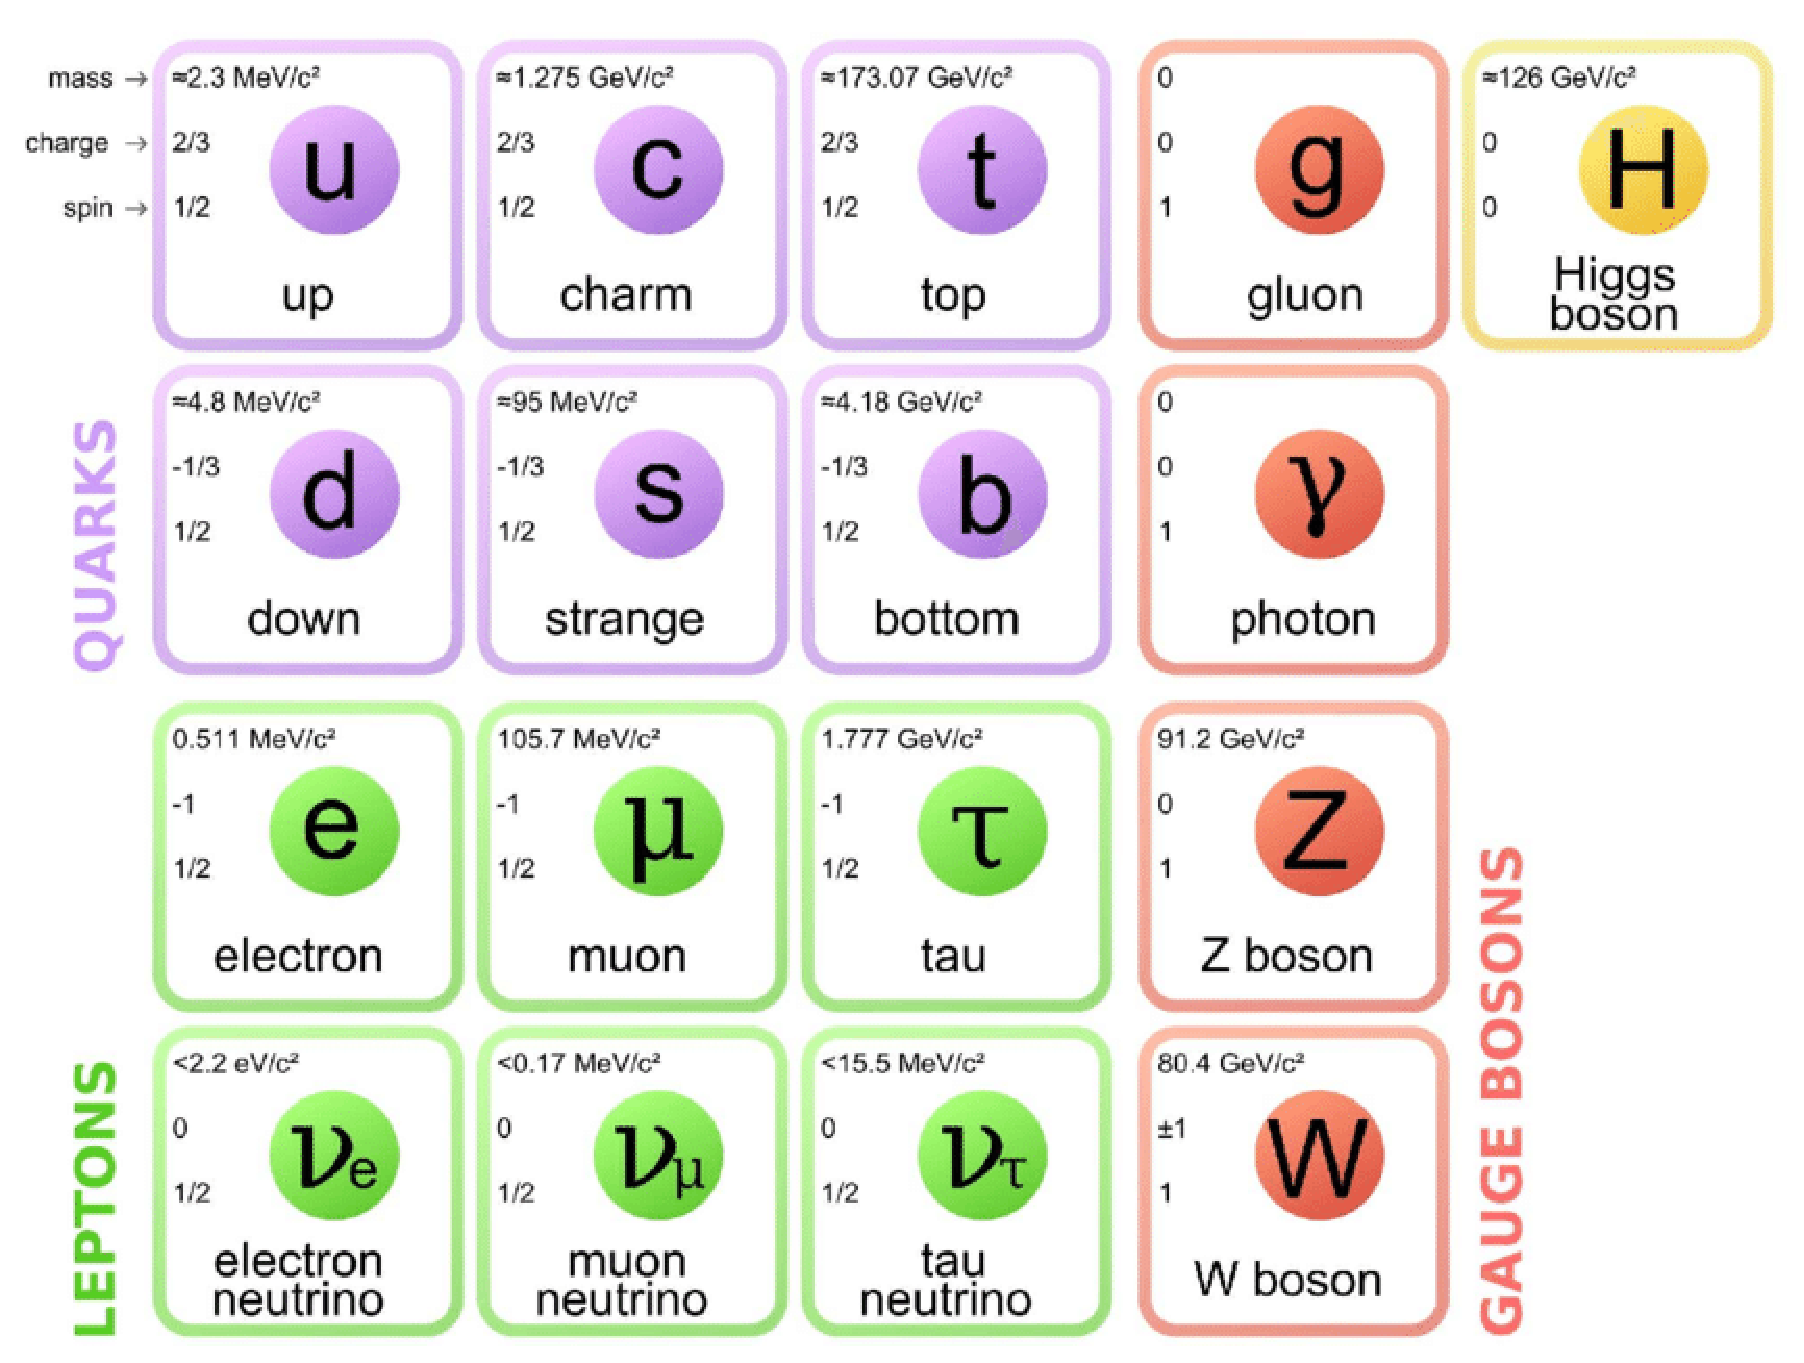
\includegraphics[scale=0.45]{Particle.eps}\\
		\caption{ The elementary particles of the SM  }
	\end{center}
\end{figure}

If an elementary particle carries the charge of a certain force, it is involved with the corresponding interaction. Quarks carry color charge (red, green, blue) and interact through the strong force mediated by massless gluons. The gluon has eight different states, which carrys a combination of color and anti-color charge in each state (color $SU(3)$ octet). The up, charm and top quarks carry a fractional electric charge of $2/3e$, while down, strange and bottom quarks carry a fractional electric charge of $-1/3e$. The charged leptons(electron, muon and tau) have an integer charge of $-e$. All electrically charged particles participate in the electromagnectic interaction mediated by the massless photon . Each charged lepton is paired with a neutral lepton (electron-, muon-, and tau-neutrino) with extremly low mass. All the particles participate in the weak interactions since they all carry an isospin, of which the $z$-compenent is either $+1/2$ (u, c, t-quark and neutrinos) or $-1/2$ (d, s, b-quark and charged leptons). The weak interactions are mediated by the neutral $Z$ or the electrically charged $W^{\pm}$ vector bosons. The masses of elementary particles in SM are acquired thorough the interactions with Higgs fields. 

In this chapter, we aim to give a brief introduction of the standard model of electroweak interactions\cite{H.P.PhyRep, BFLWQFT2, CQ}. We will introduce gauge invariance first. The spontaneous symmetry breaking and Higgs mechanism will be discussed next. Last we will review the contruction for the Lagragnian of the electroweak interactions.   


\section{Gauge Invariance}
\subsection{Abelian gauge invariance: Quantum electrodynamics}
Gauge theories are built with internal symmetries. For example, consider the $U(1)$ group of phase transformations of a free massive fermion field $\psi(x)$:
\begin{equation}
\psi(x)\to e^{-i\alpha}\psi(x),
\end{equation}
where $\alpha$ is an arbitrary phase parameter. The corresponding Lagranian density 
\begin{equation}
L(x)=\bar{\psi}(x)(i\slashed{\partial}-m)\psi(x)
\end{equation}
is invariant under these transformations. According to the N$\ddot{o}$ther theorem, this symmetry leads to a conserved current, 
\begin{eqnarray}
j_{\mu}(x)=\bar{\psi}(x)\gamma_\mu\psi(x),\hspace{2pt}
\partial^{\mu}j_\mu = 0.
\end{eqnarray}

The conserved charge,namely, generator of the $U(1)$ symmetry group, can be written as an integral over the charge density:
\begin{equation}
Q=\int d^3 x j_0(x).
\end{equation}

The invariance of the Lagragnian (1.2) under phase rotation indicates that the phase parameter $\alpha$ has no physical significance so that it could be chosen arbitrarily. It is unnatural to select a uniquely fixed $\alpha$ over all of the space-time, and it would be more natural to choose $\alpha$ locally, 
\begin{equation}
\psi(x)\to e^{-i\alpha(x)}\psi(x),
\end{equation}
where $\alpha$ depends on space-time in an arbitrary way. However, this modification brings a new problem. The Lagrangian (1.2) is no more invariant under the local phase rotations (1.5), because the derivative $\partial_\mu\psi(x)$ is transformed under phase rotation (1.5) by
\begin{equation}
\partial_\mu \psi(x)\to e^{-i\alpha(x)}\partial_\mu \psi(x)-ie^{i\alpha(x)}\partial_\mu\alpha(x)\psi(x).
\end{equation}
To solve this problem, We need to introduce a covariant derivative $D_\mu$, which has the property that $D\psi$ transforms under phase rotations like $\psi$:
\begin{equation}
D_\mu\psi(x)\to e^{-i\alpha(x)}D_\mu\psi(x).
\end{equation}

Such a covariant derivative can only be introduced if there exists another field, a vector field $A_\mu$ which interacts with the spinor field $\psi$. The covariant derivative $D_\mu$ is chosen as 
\begin{equation}
D_\mu=\partial_\mu + igA_\mu
\end{equation}
where $g$ is an arbitrary coupling constant, and $A_\mu$ transforms under a local phase transformation (gauge transformation) as follows:
\begin{equation}
A_\mu(x)\to A_\mu (x)+\frac{1}{g}\partial_\mu\alpha(x).
\end{equation}

We could easily verify that covariant (1.8) satisfies the requirement (1.7). Thus the invariance of the Lagrangian (1.2) under gauge transformations is recovered after replacing $\partial_\mu$ with $D_\mu$. However, we must add the kinetic term of the $A_\mu$ field for consistency, which must be gauge invariant in itself (only involving the gauge-invariant field strength).
\begin{equation}
F_{\mu\nu}=\partial_\nu A_\mu -\partial_\mu A_\nu.
\end{equation}

Therefore we obtain the Lagrangian which is invariant under gauge transformation
\begin{equation}
L=\bar{\psi}(i\slashed{D}-m)\psi-\frac{1}{4}F_{\mu\nu}F^{\mu\nu}.
\end{equation}
If we identify the spinor field $\psi$ with electron field, the vector field $A_\mu$ with photon field and replace $g$ by $e$ (electric charge), we obtain the Lagrangian for quantum electrodynamics (QED). Note that only the minimal coupling of the photon field to the electron field of the type $e\bar{\psi}\gamma_\mu\psi A^\mu$ is allowed due to the requirement of local gauge invariance. Furthermore a mass term for the photon filed of the type $m^2A_\mu A^\mu$ is forbidden to arise in the Lagrangian. 

\subsection{Non-Abelian gauge invariance}

The idea of non-Abelian gauge theories was formulated by Yang and Mills\cite{YM1954} in 1954. We successfully constructed the QED Lagrangian by imposing the local gauge invariance, $U(1$). This success encourages us to extend the gauge symmetry from an Abelian gauge case to a non-Abelian case. We will take the isospin symmetry as an example to formulate of the Non-Abelian gauge theories. The Lagrangian for the free protons and neutrons is 
\begin{equation}
L=\bar{N}(i\slashed{\partial}-m)N
\end{equation}
where $N$ represents the isospinor $(p,n)^T$. It is invariant under $SU(2)$ transformations
\begin{equation}
N\to e^{-i\alpha\sigma/2}N
\end{equation}
where $\sigma=(\sigma_1,\sigma_2,\sigma_3)$ ($\sigma\equiv$ Pauli matrices). and $\alpha$ is an arbitrary phase vector. The isotropic spin currents $\bar{N}\gamma_\mu\frac{1}{2}\sigma_iN$ are conserved. And the associated charges $T_i = \int d^3x \bar{N}\gamma\frac{1}{2}\sigma_iN$ generate the algebra of $SU(2)$:
\begin{equation}
[T_i, T_j] = i\epsilon_{ijk}T_k.
\end{equation} 
Note that the gauge transformations involving nondiagonal Pauli matrices $\sigma_1$, $\sigma_2$ result in the mixing between $p$ and $n$ states. However, this would not be a problem, since there would be no physical difference between proton and neutron for the isospin symmetry. Our selection for $p$ or $n$ totally depends on convention. Therefore it would be natural to redefine $p$ and $n$ locally in an arbitrary way, namely, we require the invariance under non-Abelian gauge transformations:
\begin{equation}
\binom{p}{n}\to e^{-i\alpha(x)\sigma/2}\binom{p}{n}
\end{equation} 
where $\alpha(x)$ is an arbitrary spacetime dependent phase vector. We will encounter the same problem as in the Abelian case discussed above: the derivative $\partial_\mu N$ which occurs in the Lagrangian (1.12) will not transform under local gauge transformations as $N$ itself, and we have to define a proper covariant derivative. To achieve this goal, we introduce a triplet of vector gauge fields $W_\mu^i$, which transforms under an infinitesimal gauge transformation as follows:
\begin{equation}
W_\mu^i\to W_\mu^i + \epsilon_{ijk}\alpha^j W_\mu^k+\frac{1}{g}\partial_\mu\alpha^i
\end{equation}
This transformation is analogous to eq. (1.9). The second term shows the local rotation of the $W^i$ in the isotropic space. The covariant derivative is defined as
\begin{equation}
D_\mu = \partial_\mu + igW_\mu
\end{equation}
where  $W_\mu=\frac{1}{2}\sigma W_\mu$. The Lagrangian of the system is 
\begin{equation}
L=\bar{N}(i\slashed{\partial}-m)N-\frac{1}{4}G_{\mu\nu}^i G_i^{\mu\nu},
\end{equation} 
where the $G_{\mu\nu}^i$ are the field strength tensors of the vector fields:
\begin{equation}
G_{\mu\nu}^i = \partial_\nu W_\mu^i - \partial_\mu W_\nu^i -g\epsilon^{ijk} W_{j\nu}W_{k\mu}
\end{equation}

This approach can be generalized to the case where an arbitrary gauge group and an arbitrary fermion representation are involved. The only changes are as follows:

(a) Replace the isospin matrices $\sigma$ with the corresponding matrices describing the transformation properties of the fermions under the gauge group.

(b) Replace $\epsilon_{ijk}$ with the structure constants $f_{ijk}$ of the gauge group. 

Note that the fermions can transform as an arbitrary representation of the gauge group, while the vector gauge fields must transform according to the adjoint representation. In the non-Abelian gauge theory, the vector fields interact with each other directly ("they are charged"). This is not the case in the Abelian theory where the vector field is neutral. The Lagrangian of the non-Abelian gauge theory (1.18) describes the interactions of massive fermions with massless gauge bosons.


\section{Spontaneous Symmetry Breaking}
It is known that the weak interactions are mediated by massive vector bosons $Z$ and $W^{\pm}$. However, we have seen above that the non-Abelian gauge invariance requires the gauge bosons to be massless. This means we must seek another possibility to introduce masses for the gauge fields in a more subtle way, such that the local gauge invariance is preserved. This can be realized by generating the gauge boson masses via a spotaneous breaking of the gauge symmetry. 

Usually the equations of motion for a physical system are symmetric under some symmetry transformations, however, the ground state of the systems is not. For example, the Hamiltonian for an infinitely extended ferromagnet is invariant under rotations in space. However, the ground state breaks the rotational symmetry since the individual spins are always aligned in an arbitrary direction. Similar situations arise in the field theory often, and we will discuss several examples of spontaneous breaking field theories.

The simplest example to exhibit the phenomenon of spontaneous symmetry breaking is the $\phi^4$ theory. Consider the Lagrangian
\begin{equation}
L=\frac{1}{2}(\partial^\mu \phi\partial_\mu \phi)-\frac{1}{2}\mu^2\phi^2-\frac{1}{4}\lambda\phi^4.
\end{equation}
The Lagrangian (1.20) is invariant under the parity transformation $P$, defined by $\phi\stackrel{P}{\to} -\phi$. The ground state (vacuum state $\Ket{0}$) of the theory is the one where $\phi$ vanishes everywhere. It is invariant under the parity transformation: $P\Ket{0}=\Ket{0}$. 

\begin{figure}
	\begin{center}
		\includegraphics[scale=0.08]{index.eps}\\
		\caption{The potential V($\phi$) of the scalar field $\phi$ in the case $\mu^2>0$ (left) and $\mu^2>0$ (right)  }
	\end{center}
\end{figure}

If the parameter $\mu^2>0$, the potential $V(\phi)=\frac{1}{2}\mu^2\phi^2+\frac{1}{4}\lambda\phi^4$ has a unique minimum at $\phi=0$, as shown in Figure 1.2, which corresponds to the vacuum state. 

If the parameter $\mu^2>0$, the situation is that of a spontaneously broken symmetry. The potential 
\begin{equation}
V(\phi)=-\frac{1}{2}|\mu^2|\phi^2+\frac{1}{4}|\lambda|\phi^4,
\end{equation}
shown in Figure 1.2, has minima at 
\begin{equation}
\Bra{0}\phi\Ket{0} = \pm\sqrt{-\mu^2/|\lambda|}\equiv \pm v,
\end{equation}
which corresponds to two possible ground states. These vacuums are not invariant under parity transformation since $v \neq -v$. Thus the parity invariance is spontaneously broken. It is useful to define a new field $\phi'$, for which $\Bra{0}\phi'\Ket{0}$=0, i.e. $\phi'=\phi-v$. In terms of $\phi$ we have 
\begin{equation}
L=\frac{1}{2}(\partial^\mu \phi'\partial_\mu \phi')-\mu^2\phi'^2-\frac{1}{4}\lambda\phi'^4-\lambda v\phi^3+\text{const}.
\end{equation}

We see that the Lagrangian (1.20) with $\mu^2<0$ describes self-interacting scalar particles with mass $\sqrt{2}|\mu|$. 




Next, let us consider the theory of a complex scalar field $\phi =\frac{\sqrt{2}}{2}(\phi_1+i\phi_2)$. Consider the Lagrangian
\begin{align}
L&=\frac{1}{2}(\partial^\mu \phi^{\ast} \partial_\mu \phi)-\frac{1}{2}\mu^2\phi^2-\frac{1}{4}\lambda\phi^4\nonumber\\
&=\frac{1}{2}\partial^\mu\phi_1\partial_\mu\phi_1+\frac{1}{2}\partial^\mu\phi_2\partial_\mu\phi_2-\frac{1}{2}\mu^2(\phi_1^2+\phi_2^2)-\frac{1}{4}\lambda(\phi_1^2+\phi_2^2)^2.
\end{align}

It is invariant under the phase transformation $\phi \to e^{-i\theta}\phi$. For $\mu^2>0$ this Lagrangian describes a self-interacting scalar complex field of mass $\mu$. 

Assume we choose $\mu^2<0$ now, then the potential $V(\phi)$ has a minimum at $(\phi_1^2+\phi_2^2)=2|\phi|^2=-\mu^2/\lambda$. So the minimum of the potential occurs along a circle of radius $\sqrt{-\mu^2/\lambda}$ around the origin. Because we could pick any point on the circle as the vacuum state, we are now dealing with an infinite number of possible vacua. Let us take an arbitrary point on the circle as the vacuum, described by the coordinates $v=(v_1,v_2)$. Since the Lagrangian is invariant under phase transformations, we could let this point lie on the 
positive real axis, namely, $v=(\sqrt{-\mu^2/\lambda})$, which implies $\Bra{0}\phi_1\Ket{0}=\sqrt{-\mu^2/\lambda}$, $\Bra{0}\phi_2\Ket{0}=0$.

Now we define $\phi_1'=\phi_1-\Bra{0}\phi_1\Ket{0}$, then the Lagrangian (1.24) becomes
\begin{equation}
L=\frac{1}{2}\partial^\mu\phi'_1\partial_\mu\phi'_1+\frac{1}{2}\partial^\mu\phi_2\partial_\mu\phi_2+\mu^2{\phi'_1}^2-\frac{1}{2}\lambda v\phi'_1({\phi'_1}^2+{\phi_2}^2)-\frac{\lambda}{4}({\phi'_1}^2+{\phi_2}^2)^2,
\end{equation}
where $v=\sqrt{-\mu^2/\lambda}$. From the Lagrangian (1.25), we see that the field $\phi_1$ describes a particle of mass $\sqrt{2|\mu|}$, but $\phi_2$ is still massless.

The system described above gives an example of the Goldstone theorem \cite{Nambu,NambuLasinio1,NambuLasinio2,Goldstone,Bludman}: for every spontaneously broken continuous symmetry, the theory contains massless Goldstone bosons (spin-$0$).

The example discussed above exhibits an invariance under the global gauge group $U(1)$ which is isomorphic to $O(2)$. It could be generalized to involve the gauge group $O(n)$. Let us consider the Lagrangian
\begin{eqnarray}
&&L=\frac{1}{2}(\partial^\mu \phi_i\partial_\mu \phi_i)-\frac{1}{2}\mu^2\phi_i\phi_i-\frac{1}{4}\lambda(\phi_i\phi_i)^2, i = 1,2,\cdots,n;\nonumber\\
&& \phi_i \equiv \text{real scalar field}; \text{ summation over $i$}.
\end{eqnarray}
This Lagrangian is invariant under the group $O(n)$. For $\mu^2<0$ the minimum of the potential is at $v=\sqrt{-\mu^2/\lambda}$. The potential $V(\phi)$ exhibits the minimum at $\phi_i\phi_i=-\mu^2/\lambda$, i.e. it arises on the $n$-dimensional sphere of radius $\sqrt{-\mu^2/\lambda}$ in the $n$-dimensional space defined by the fields $\phi_i$. Because of the $O(n)$-invariance of the Lagrangian we could select the coordinates of fields so that the vacuum expectation value of the field vector $\phi_i$ is defined as follows:
\begin{equation}
\bra{0}\phi\ket{0}=
\begin{bmatrix}
0\\0\\0\\\vdots\\0\\v
\end{bmatrix}.
\end{equation}

Note that the first $(n-1)$ components of $\bra{0}\phi\ket{0}$ are zero, the vacuum remains invariant under the subgroup $O(n-1)$. We see that the vacuum expectation value $\bra{0}\phi\ket{0}$ breaks the $O(n)$-invariance in a particular way. Let us see the point (1.27) in the n-dimensional space of the fields $\phi_i$. There are $(n-1)$ linearly independent directions to leave this point, but to stay on the sphere which minimizes the potential. Therefore there must exist $(n-1)$ massless Goldstone bosons, according to the Goldstone theorem. So the Lagrangian (1.26) describes a massive field of mass $\sqrt{-2\mu^2}$ and $(n-1)$ massless Goldstone bosons.

The group $O(n)$ has $\frac{1}{2}n(n-1)$ generators, while the subgroup $O(n-1)$ has $\frac{1}{2}(n-1)(n-2)$ generators. This means $(n-1)$ generators of $O(n)$ do not leave the vacuum invariant. On the other hand, we have $(n-1)$ massless Goldstone bosons, namely, the number of massless Goldstone bosons is equal to the number of generators which are broken spontaneously. This feature is a special property of the $O(n)$ model we have discussed above, but a general feature of spontaneously broken theories involving scalar fields. The number of Goldstone bosons corresponds always to the number of the spontaneously broken generators as a consequence of the general Goldstone theorem\cite{AbersLee}.
\newpage
\section{The Higgs Mechanism}
As we discussed above, the local gauge invariance requires gauge bosons to be massless only. However, in reality, the observed gauge bosons of weak interactions $Z$ and $W^{\pm}$ are massive. In order to reconcile this contradiction, we need to incorporate Higgs mechanism\cite{Higgs1,Higgs2,Higgs3} into the gauge theory, by which spontaneous symmetry breaking generates a mass for a gauge boson. 

\subsection{The Higgs Mechanism in the Abelian Theory}
Let us consider the Lagrangian 
\begin{equation}
L=\partial^\mu \phi^{\ast}\partial_\mu\phi-\mu^2\phi^{\ast}\phi-\lambda(\phi^{\ast}\phi)^2,
\end{equation}
which is invariant under the global gauge transformations $\phi\to e^{-i\alpha}\phi$, i.e., $U(1)$ gauge group. However, we need invariance under the local gauge transformations $\phi\to e^{-i\alpha(x)}\phi$. In order to achieve this goal, we need to introduce a gauge field $A_\mu$. Repeating the procedure outlined in Subsection 1.1.1, we arrive at 
\begin{equation}
L=(D^\mu \phi)^{\ast}D_\mu\phi-\mu^2\phi^{\ast}\phi-\lambda(\phi^{\ast}\phi)^2-\frac{1}{4}F_{\mu\nu}F^{\mu\nu},
\end{equation}
where $F_{\mu\nu}=\partial_\nu A_\mu - \partial_\mu A_\nu$, and $D_\mu=\partial_\mu+igA_\mu$.

We note that the various fields transform under local gauge transformations as follows:
\begin{eqnarray}
&&\phi(x)\to e^{-i\alpha(x)}\phi(x),\nonumber\\
&&A_\mu (x)\to A_\nu (x)+\frac{1}{g}\partial_\mu\alpha(x).
\end{eqnarray}

For $\mu^2>0$ the Lagrangian (1.29) describes the system of a massive scalar field, coupled to a massless gauge field $A_\mu$. If we let $g=e$(electric charge), then we are dealing with the scalar electrodynamics.  

For $\mu^2<0$ the gauge symmetry is spontaneously broken, as discussed in Section 1.2. We have known that the Lagrangian (1.28) describes a massive scalar field, accompanied by a massless Goldstone by following the approach outlined in section 1.2. Next, we will investigate what will happen in case of the  gauge invariant Lagrangian (1.29). Let us make the substitution
\begin{equation}
\phi_1=\phi'_1+\bra{0}\phi_1\ket{0}=\phi_1+v, v=\sqrt{-\mu^2/\lambda}
\end{equation} 
in eq. (1.29). We therefore expand the scalar field $\phi(x)$ around the vacuum expectation value $\bra{0}\phi\ket{0}$ and arrive at
\begin{equation}
L=-\frac{1}{4}F_{\mu\nu}F^{\mu\nu}+\frac{1}{2}\partial^\mu \phi_1\partial_\mu\phi_1+\frac{1}{2}\partial^\mu \phi_2\partial_\mu\phi_2+\frac{1}{2}g^2v^2 A_\mu A^\mu - gvA_\mu\partial^\mu\phi_2.
\end{equation}

We find that following new terms arise:
\begin{equation}
\frac{1}{2}g^2v^2 A_\mu A^\mu,
\end{equation}
\begin{equation}
 - gvA_\mu\partial^\mu\phi_2.
\end{equation}
The term (1.33) could be interpreted as the gauge boson mass term where the mass $m_A^2 = g^2v^2$ arises from the nonvanishing vacuum expectation value of $\phi$. However, the interpretation of the term (1.34) is sort of vague, since it mixes the gauge field with the Goldstone boson $\phi$. In order to clarify this condition, let us consider the gauge transformation $\phi\to e^{-i\alpha}\phi$ in terms of $\phi'_1$ and $\phi_2$.

For an infinitesimal parameter $\alpha$ we have
\begin{eqnarray}
&&\phi\to(1-i\alpha)\phi,\nonumber\\
&&\phi_1\to\phi_1-\alpha\phi_2,\nonumber\\
&&\phi_2\to\phi_2+\alpha\phi_1,
\end{eqnarray}
and we find
\begin{eqnarray}
&&\phi'_1\to\phi'_1-\alpha\phi_2,\nonumber\\
&&\phi_2\to\phi_2+\alpha v+\alpha\phi'_1,
\end{eqnarray}

Thus $\phi_2$ undergoes an inhomogenous gauge transformation like the gauge field $A_\mu$. So we could use the freedom of gauge to set $\phi_2=0$, in which the mixing term (1.34) and the Goldstone boson vanish. 

As we see, the introduction of the gauge field $A_\mu$ and the requirement of local gauge invariance fully change the physical condition: the Lagrangian (1.28) describes a massive scalar field accompanied with a massless Goldstone boson, while the Lagrangian (1.29) describes a massive gauge boson $A_\mu$ and a massive scalar boson $\phi$. However, the total number of the particle states remains unchanged. Before spontaneous symmetry breaking, the theory had four particle states: two spin-zero particles $\phi$ and $\phi^{\ast}$ plus two polarization states of the massless gauge boson $A_\mu$, i.e. four states in total. After spontaneous symmetry breaking, we have one scalar particle plus three polarization states of the massive gauge boson $A_\mu$, i.e. still four states. Therefore, we could say that the massless gauge boson "ate" the massless Goldstone boson to become a massive gauge boson. 


The Higgs mechanism introduced above is important for the following discussion. In general theories involving massive gauge bosons are non-renormalizable, because of the $k_\mu k_\nu/m^2$-term in the gauge boson propagator. However, in the original Lagrangian (1.29), the gauge field is formally massless, where no issues with renormalizability occurs. It turns out that spontaneous symmetry breaking would not affect the renormalizibility of the theory\cite{thooft1,thooft2,tHooftVeltman}. Note that for the Abelian gauge theory described by the Lagrangian (1.28), the spontaneous generation of the gauge boson mass is not necessary to achieve renormalizability. We would not undermine the renormalizablity if we introduce a mass term for the gauge boson, provided that the gauge field $A_\mu$ is coupled with a conserved current. However, this is not valid for a non-Abelian theory. The spontaneous generation of gauge boson masses is the only way to ensure renormalizability.

In sum, Higgs meachanism is a remarkable result, suggesting the possibility of establishing spontaneously broken gauge theories in which the interactions are mediated by massive gauge bosons. 
 

\subsection{The Higgs Mechanism in the non-Abelian Theory}
In order to explore additional complications from spontaneous symmetry breaking of a non-Abelian theory, we choose $SU(2)$ gauge theory as a prototype.

At first, we choose a doublet representation of complex scalar fields, coupled to the gauge fields in a gauge invariant way. Such a Lagrangian is defined by
\begin{equation}
L=-\frac{1}{4}G^i_{\mu\nu}G_i^{\mu\nu}+\Big(\partial^\mu\phi+i\frac{g}{2}\sigma^iB^{\mu i}\phi\Big)^{\dagger}
\Big(\partial_\mu\phi+i\frac{g}{2}\sigma_i B_{\mu}^i\phi\Big)-\mu^2\phi^{\dagger}\phi-\lambda(\phi^{\dagger}\phi)^2,
\end{equation}
where the scalar field $\phi$ represents the $SU(2)$ doublet
\begin{equation}
\phi=\binom{\phi_a}{\phi_b},
\end{equation}
and the $\sigma_i$'s denote the Pauli matrices.

For $\mu^2>0$ the Lagrangian (1.37) describes a system of massless gauge fields in interaction with massive scalars of mass $\mu$. Now suppose we choose $\mu^2<0$, then  the potential $V(\phi)=\mu^2\phi^\dagger\phi+\lambda(\phi^\dagger\phi)^2$ exhibits its minimum at finite values of $\phi$. The manifold of points in the space of fields $\phi_a$, $\phi_b$ for which the minimum of the potential $V(\phi)$ occurs is invariant under $SU(2)$-transformations. Therefore, we could choose a specific $SU(2)$ frame for which we have $\bra{0}\phi\ket{0}=\frac{1}{\sqrt{2}}\binom{0}{v}$, where $v=\sqrt{-\mu^2/\lambda}$. Form eq. (2.35) we obtain the mass term of the gauge field, which is
\begin{align}
\frac{g^2}{4}[(\sigma^i B^i_\mu)]^{\dagger}[(\sigma^i B^i_\mu)]&=\frac{g^2}{4}(\phi^\dagger\tau^j\tau^i\phi)(B_\mu^i B^{\mu i})\nonumber\\
&=\frac{g^2}{8}\cdot v^2[(B^1_\mu)^2+(B^2_\mu)^2+(B^3_\mu)^2].
\end{align}

Thus we could conclude: we obtain massive gauge fields after spontaneous symmetry breaking. The gauge boson mass matrix is $SU(2)$ symmetric, namely, the three gauge bosons are degenerate in mass. This is a special feature of the spontaneous symmetry breaking involving an $SU(2)$ doublet.

Note that the particle content of the theory includes three massive gauge fields and one massive scalar field. Three of the scalar fields (four real fields originally) have been eaten to provide the longitudinal components of the massive gauge fields. 

Next, we choose an $SU(2)$ triplet representation of real scalar fields
\begin{equation}
\phi=\left(
\begin{array}{c}
\phi_1\\ \phi_2\\ \phi_3
\end{array}
\right).
\end{equation}
We require invariance under the gauge transformation
\begin{equation}
\phi\to e^{iT_i \alpha_i}\phi,
\end{equation}
where the exponential factor is a $3\times3$ matrix. The operator $T_i$ generates isospin rotations about the $i$-axis and satisfies the usual $SU(2)$ algebra
\begin{equation}
[T^j,T^k]=i\epsilon_{jkl}T^l.
\end{equation}
The explicit matrix representation is 
\begin{equation}
(T^j)_{kl} = -i\epsilon_{jkl}.
\end{equation}

Following the procedure outline in Section 1.2, we have the covariant derivative as follows
\begin{equation}
D_\mu = \partial_\mu - igT_i B_{\mu i},
\end{equation}
or, in the ajoint representation, the covariant derivative takes the form,
\begin{equation}
(D_\mu)_{kl}=\delta_{kl}\partial_\mu + g\epsilon_{jkl}B_{\mu j}.
\end{equation}
Then the Lagrangian of the theory is 
\begin{equation}
L=-\frac{1}{4}G^i_{\mu\nu}G_i^{\mu\nu}+\frac{1}{2}(\partial^\mu\phi_i-g\epsilon_{ijk}B^\mu_j\phi_k)
(\partial_\mu\phi_i-g\epsilon_{ilm}B^\mu_l\phi_m)-\frac{1}{2}\mu^2\phi_i\phi_i-\frac{1}{4}\lambda(\phi_i\phi_i)^2.
\end{equation}

When $\phi$ is the unique minima of the potential $V(\phi)=\frac{1}{2}\mu^2\phi_i\phi_i+\frac{1}{4}\lambda(\phi_i\phi_i)^2$, the spectrum is that of an ordinary, isospin-conserving gauge filed theory: three massive scalar fields, each with mass $\mu$, and three massless gauge fields $B_\mu$. Since each massless gauge boson has two polarization states, then the number of particle states is $3\times1+3\times2=9$. 

If we choose $\mu^2<0$, spontaneous symmetry breaking occurs. We could choose a particular coordinate system of fields such that we have 
\begin{equation}
\bra{0}\phi\ket{0}=\left(
\begin{array}{c}
0\\0\\v
\end{array}\right).
\end{equation} 

This vector remains invariant under rotation generated by $T_3$, i.e. the subgroup $U(1)\subset SU(2)$, generated by the third generator $T_3$ remains unbroken.

We shift the scalar fields and expand around the $v$, using 
\begin{eqnarray}
\phi \to \exp\biggl[\frac{i}{v}(\zeta_1 T_1+\zeta_2 T_2)  \biggr]
\left(
\begin{array}{c}
	0\\0\\v+\eta
\end{array}
\right).
\end{eqnarray}

We could exploit the gauge invariance of the theory by letting
\begin{eqnarray}
\phi \to \exp\biggl[-\frac{i}{v}(\zeta_1 T_1+\zeta_2 T_2)  \biggr]
\phi=\left(
\begin{array}{c}
0\\0\\v+\eta
\end{array}
\right).
\end{eqnarray}
With the help of the new gauge, we obtain the Lagrangian
\begin{equation}
L=\frac{1}{2}(\partial_\mu\eta\partial^\mu\eta+2\mu^2\eta^2)-\frac{1}{4}G_{\mu\nu}^i G^{\mu\nu i}+\frac{1}{2}g^2v^2[B^1_\mu B^{1\mu}+B^2_\mu B^{2\mu}]+\cdots
\end{equation}

From this Lagrangian, we conclude: $\eta$ has become a massive Higgs scalar field, with mass $\sqrt{-2\mu^2}$; the Goldstone bosons $\eta_1$ and $\eta_2$ have disappeared completely, i.e., they have been eaten up by gauge fields; the gauge bosons $B^{\mu}_1$ and $B^\mu_2$ respective coupled to the broken generators $T_1$ and $T_2$ have acquired a common mass $gv$; the gauge boson $B^\mu_3$ remains massless, reflecting the invariance of the vacuum under the generator $T_3$.


\section{Standard Model of the electroweak interactions}
\subsection{The General Ideas for Building Spontaneous Broken Gauge Theories }
After investigating the examples above, we are ready to discuss the general features of spontaneous broken gauge theories. Let us consider a Lagrangian which is invariant under local gauge transformations of a group $G$. The generatos $T_i$ follow the commutation relations
\begin{equation}
[T_i, T_j]=if_{ijk}T_k,
\end{equation}
where $i,j,k = 1,\cdots,N$ and $f_{ijk}$ is the structure constant of $G$. An arbitrary infinitesimal transformation of the group $G$ could be parametrized by $1-i\epsilon_i T_i$, where $\epsilon_i$'s are infinitesimal parameters.

The scalar field $\phi$ is assumed to transform under a $n$-dimensional representation of G. We assume that the field $\phi$ are real, since a complex field $\phi$ can always be decomposed into two real ones. For an infinitesimal transformation of $G$ we have:
\begin{equation}
\delta \phi=i\epsilon_i S_i\phi.
\end{equation}
The Lagrangian is defined by
\begin{equation}
L=-\frac{1}{4}G^i_{\mu\nu}G_i^{\mu\nu}+\frac{1}{2}[(\partial^\mu +igS_iA_i^\mu)\phi]^{\dagger}[(\partial_\mu +igS_jA_{j\mu})\phi]-V(\phi),
\end{equation}
where $V(\phi)$ is a quartic potential in $\phi$, invariant under $G$.

We assume that spontaneous symmetry breaking occurs and the potential exhibits its minimum at $\phi=v$, where $v$ is a $n$-dimensional vector. The gauge boson mass matrix is then given by 
\begin{equation}
(M^2)_{ij}=-g^2(S_i v)\cdot (S_j v).
\end{equation}

In general, there will exist a $M$-dimensional subgroup $G'$ of $G$, which preserves an invariance of the vacuum. 

Let $T_i(G')$ be the generators of $G'$, then $T_i(G')v=S_i(G')v=0$. There exist $(N-M)$ generators of $G$, for which $T_i v\ne0$, i.e. one has $(N-M)$ Goldstone bosons. Therefore the $N\times N$ dimensional mass matrix denoted in eq.(1.54) is actually an $(N-M)\times(N-M)$ dimensional matrix, if we leave out all terms for which $S_i v=0$ because of the $S$-invariance of the vacuum. The mass matrix (1.54) needs to be diagonalized if we would like to find the massive vector bosons of definite mass. There exist $(N-M)$ massive gauge bosons. The $(N-M)$ Goldstone bosons are aborbed into the longitudinal components of the $(N-M)$ massive gauge bosons.   

Up to now, our discussion mainly focuses on scalar and vector fields. Next, we need to incorporate fermion fields into the gauge theory, by adding to the Lagrangian (1.53) the terms
\begin{equation}
L^{\text{fermion}}=\bar{\psi}_L(i\slashed{\partial}-gf_{Li}\slashed{A}_i)
\psi_L+\bar{\psi}_R(i\slashed{\partial}-gf_{Ri}\slashed{A}_i)
\psi_R-(m\bar{\psi}_R\psi_L+\text{h.c.})
\end{equation} 
and
\begin{equation}
L^{\text{int}}=-G\bar{\psi}_R(R\phi)\psi_L+h.c.
\end{equation}
where $\psi_L$, $\psi_R$ stand for the left-handed and right-handed fermion fields. The fields $\psi_L$ and $\psi_R$ transform under G as certain irreducible representations. The matrices $f_L$, $f_R$ denote the transformation properties of the left-handed and right-handed fermion fields. In eq. (2.55), we include the Yukawa interaction term of the fermion fields with the scalar fields. The matrices $R$ are constructed so that $\bar{\psi}_R(R\phi)\bar{\psi}_L$ is invariant under the gauge group. We also include a bare mass term $(m\bar{\psi}_R\psi_L+h.c.)$, which must be $G$-invariant. 

From the eqs. (1.55) and (1.56) we obtain the fermion mass matrix after the spontaneous symmetry breaking,
\begin{equation}
L^{\text{fermion mass}}=-G\bar{\psi}_R(Rv)\psi_L-m\bar{\psi}_R\psi_L+h.c.
\end{equation}

After introducing the general properties of spontaneous broken gauge theories, we are ready to give the general recipe for building renormalizable gauge theories. The Lagrangian is constructed as follows:

1. Select the gauge group, the representations of left-handed and right-handed fermions and the scalar fields.

2. Couple the gauge fields invariantly to the fermion and scalar fields.

3. Couple the gauge invariant quartic polynomial of the scalar fields so that the potential reaches its minimum for nonvanishing vacuum expectation values $v$.

4. Construct the gauge invariant Yukawa couplings between the fermions and scalars.

The gauge boson mass matrix has the structure: 
$$
\frac{1}{2}g^2v^2W_\mu^2,
$$
the fermion mass matrix is
$$
G\cdot v\bar{\psi}\psi.
$$

\subsection{The Glashow-Weinberg-Salam Theory of Electroweak Interations}
We are now ready to write down the spontaneously broken gauge theory that gives experimentally confirmed description of weak and electromagnetic interactions, a model introduced by Glashow, Weinberg, and Salam (GWS) \cite{Glashow1961,Weinberg,Salam}. We begin with the doublet of the weak isospin consisting of left-handed electron and its neutrino,
\begin{equation}
\psi_{L}^e \equiv \binom{\nu_e}{e}_L,
\end{equation}
where the left-handed states are
\begin{align}
\nu_L&=\frac{1}{2}(1-\gamma_5)\nu_e\nonumber\\
e_L&=\frac{1}{2}(1-\gamma_5)e
\end{align}
The electron neutrino is known to be nearly massless. It is convenient to idealize it as exactly massless, in which case the right-handed state 
\begin{eqnarray}
\nu_R = \frac{1}{2}(1+\gamma_5)\nu_e
\end{eqnarray}
does not exist. Thus we have only one right-handed fermion,
\begin{equation}
\psi_R^e \equiv e_R =\frac{1}{2}(1+\gamma_5)e,
\end{equation}
which is an $SU(2)$-singlet.

Note that we need to have the $U(1)$-factor in the gauge group $SU(2)\otimes U(1)$ to represent the electric charge. This cannot be an $SU(2)$ generator since the photon couples both to the left-handed and right-handed electron. To incorporate the electromagnetic interaction, we denote the $U(1)$ generator as ``weak hypercharge", $Y$. Requiring that the Gell-Mann-Nishijima relation for electric charge,
\begin{equation}
Q=I_3+\frac{1}{2}Y
\end{equation}
be satisfied leads to the assignments
\begin{eqnarray}
&&Y_L =-1,\nonumber\\
&&Y_R = -2.
\end{eqnarray}
By construction, the weak-isopin projection $I_3$ and the weak hypercharge $Y$ commute:
\begin{equation}
[I_3,Y]=0.
\end{equation}
Let us take the group of transformations generated by $I$ and $Y$ to be the gauge group $SU(2)_L\otimes U(1)_Y$ for the gauge theory. In order to construct the theory, we introduce the gauge bosons $A_\mu^1$, $A_\mu^2$, $A_\mu^3$ for $SU(2)_L$ and $B_\mu$ for $U(1)_Y$.

The Lagrangian for the theory might be written as
\begin{equation}
L=L^{\text{gauge}}+L^{\text{fermion}}+L^{\text{scalar}},
\end{equation}
and the gauge boson part of the Lagrangian is
\begin{equation}
L^{\text{gauge}}=-\frac{1}{4}F^l_{\mu\nu}F_l^{\mu\nu}-\frac{1}{4}G_{\mu\nu}G^{\mu\nu}
\end{equation}
where 
\begin{equation}
F^l_{\mu\nu}=\partial_\nu A^l_\mu-\partial_\mu A^l_\nu+g\epsilon_{jkl} A^j_{\mu} A^k_{\nu}
\end{equation}
for the $SU(2)_L$ gauge fields and
\begin{equation}
G_{\mu\nu}=\partial_\nu B_\mu -\partial_\mu B_\nu
\end{equation}
for the $U(1)_Y$ gauge field. 

We introduce a complex doublet of scalar fields
\begin{eqnarray}
\phi\equiv\binom{\phi^{\dagger}}{\phi_0}
\end{eqnarray}
which transforms as an $SU(2)_L$ doublet and has the hypercharge 
\begin{equation*}
Y_\phi=1
\end{equation*}
by virtue of the Gell-Mann-Nishijima relation.

Now we are ready to write down the fermion and scalar parts of the Lagrangian:
\begin{equation}
L^{\text{fermion}}=\bar{\psi}_R^e\bigg(\slashed{\partial} +\frac{ig'}{2}\slashed{B}Y\bigg)\psi_R^e+\bar{\psi}_L^e i\bigg( \slashed{\partial}+\frac{ig'}{2}\slashed{B}Y+\frac{ig}{2}\sigma_i\slashed{A}_i  \bigg)\psi_{L}^e
\end{equation}
and 
\begin{equation}
L^{\text{scalar}}=(D^\mu \phi)^{\dagger}(D_\mu\phi)-V(\phi^{\dagger}\phi),
\end{equation}
where the covariant derivative is
\begin{equation}
D_\mu =\partial_\mu +\frac{ig'}{2}B_\mu Y +\frac{ig}{2}\sigma_i A_{i\mu }
\end{equation}
and the most general form of the potential is 
\begin{equation}
V(\phi^\dagger\phi)=\mu^2(\phi^\dagger\phi)+|\lambda|(\phi^\dagger\phi).
\end{equation}
We also add an interaction term, which involves Yukawa couplings of the scalar to the fermions,
\begin{equation}
L^{\text{Yukawa}}=-G_e [\bar{\psi}_R^e(\phi^\dagger\psi_{L}^e)+(\bar{\psi}_L^e)\psi_R^e],
\end{equation}
which is symmetric under $SU(2)_L\otimes U(1)_Y$ transformations,

Now let us take $\mu^2<0$, then the $SU(2)_L\otimes U(1)_Y$ symmetry is spontaneously broken.  We choose a $SU(2)$ frame so that the vacuum expectation values of $\phi$ take the form:
\begin{equation}
\bra{0}\phi\ket{0}=\binom{0}{v/\sqrt{2}},
\end{equation}
where $v=\sqrt{-\mu^2/|\lambda|}$, which breaks both $SU(2)_L$ and $U(1)_Y$ symmetries. However, the electric charge, which is a linear combination of $T_3$ and $Y$ remains unbroken. The photon will therefore remain massless, while three other gauge bosons will aquire mass.

We next expand the Lagrangian about the minimum of the Higgs potential $V$ by letting
\begin{equation}
\phi=\exp\bigg(\frac{i\zeta_i\sigma_i}{2v} \bigg)\binom{0}{(v+\eta)/\sqrt{2}}
\end{equation}
and transforming to U-gauge:
\begin{equation}
\phi\to \exp\bigg(-\frac{i\zeta_i\sigma_i}{2v} \bigg)\phi=\binom{0}{(v+\eta)/\sqrt{2}},
\end{equation}
\begin{equation}
\sigma_i A_{i\mu}\to \sigma_i A'_{i\mu},
\end{equation}
\begin{equation}
B_\mu \to B_\mu,
\end{equation}
\begin{equation}
\psi_R^e \to \psi_R^e,
\end{equation}
\begin{equation}
\psi_L \to \exp\bigg(-\frac{i\zeta_i\sigma_i}{2v} \bigg)
\end{equation}

We now express the Lagrangian in terms of the U-gauge fields (1.77-1.81) and explore the results of spontaneous symmetry breaking. The Yukawa part of Lagrangian has become
\begin{eqnarray}
L^\text{Yukawa} = -G_e\frac{v+\eta}{\sqrt{2}}(\bar{e}_R e_L+\bar{e}_L e_R)=-\frac{G_e v}{\sqrt{2}}\bar{e}e-\frac{G_e \eta}{\sqrt{2}}\bar{e}e
\end{eqnarray}
so the electron has aquired a mass
\begin{equation}
m_e = G_e v/\sqrt{2}
\end{equation}

The scalar part of the Lagrangian now becomes
\begin{equation}
L^\text{scalar} =\frac{1}{2}(\partial^\mu\eta)(\partial_\mu\eta)-\mu^2\eta^2+\frac{v^2}{8}[g^2|A^1_\mu-iA^2_\mu|^2+(g'B_\mu-gA_\mu^3)^2]+\cdots
\end{equation}
We see immediately that the $\eta$ field has acquired a mass $m_H=\sqrt{-2\mu^2}$; it is the physical Higgs boson. If we define the charged gauge fields
\begin{equation}
W_\mu^\pm\equiv \frac{A_\mu^1\mp A_\mu^2}{\sqrt{2}},
\end{equation}
the term proportional to $g^2 v^2$ is identified as a mass term for the charge gauge bosons:
\begin{equation}
\frac{g^2v^2}{8}(|W_\mu^+|^2+|W_\mu^-|^2),
\end{equation}
corresponding to charged boson masses
\begin{equation}
M_{W_\pm}=gv/2.
\end{equation}

Then, defining the orthogonal combinations
\begin{equation}
Z_\mu=\frac{-g'B_\mu+gA^3_\mu}{\sqrt{g^2+g'^2}}
\end{equation}
and
\begin{equation}
A_\mu=\frac{gB_\mu+g'A^3_\mu}{\sqrt{g^2+g'^2}}
\end{equation}
we see that the netural boson has aquired a mass
\begin{equation}
M_{Z^0}=\sqrt{g^2g'^2}v/2=M_W\sqrt{1+g'^2/g^2}
\end{equation}
and that the gauge field $A_\mu$ remains massless. 

Next, let us investigate the interactions. We could read off the interations among the gauge bosons and fermions from $L^\text{fermion}$. For the charged gauge bosons we have 
\begin{align}
L^{W-f}&=-\frac{g}{\sqrt{2}}(\bar{\nu}_L\gamma_\mu e_L W_\mu^+\bar{e}_L\gamma^\mu\nu_L W_\mu^-)\nonumber\\
&=-\frac{g}{2\sqrt{2}}[\bar{nu}\gamma_\mu(1-\gamma_5)eW_\mu^+\bar{e}\gamma_\mu(1-\gamma_5)\nu W_\mu^-],
\end{align}
where we identify the couling constant as
\begin{equation}
\frac{g^2}{8} =\frac{G_f M_W^2}{\sqrt{2}}.
\end{equation}
with $G_f$ is the Fermi constant.
Similarly, the neutral gauge boson couplings to fermions are given by
\begin{align}
L^\text{0-f}=&\frac{gg'}{\sqrt{g^2+g'^2}}\bar{e}\gamma_\mu e A_\mu-\frac{\sqrt{g^2+g'^2}}{2}\bar{\nu}_L\gamma_\mu\nu_L Z_\mu
+\frac{Z_\mu}{\sqrt{g^2+g'^2}}\nonumber\\
&+\frac{Z_\mu}{\sqrt{g^2+g'^2}}\biggl[-g'^2\bar{e}_R\gamma_\mu e_R +\frac{(g^2-g'^2)}{2}\bar{e}_L \gamma_\mu e_L \biggr].
\end{align}
Thus we can identify $A_\mu$ as the photon, setting
\begin{equation}
\frac{gg'}{\sqrt{g^2+g'^2}}=e.
\end{equation}

It is convenient to introduce a weak mixing angle $\theta_W$ to parametrize the mixing of the neutral gauge bosons. Defining 
\begin{equation}
g'=g\tan\theta_W, \quad \sin\theta_W=\frac{g'}{g^2+g'^2},
\end{equation}
we could rewrite eqs. (1.88) and (1.89) as
\begin{align}
Z_\mu &= -B_\mu\sin\theta_W+ A_\mu^3\cos\theta_W,\nonumber\\
A_\mu &= -A_\mu\cos\theta_W+ A_\mu^3\sin\theta_W.
\end{align}

By the virtue of the relation (1.95), the coupling constants of the $SU(2)_L$ and $U(1)_Y$ gauge groups might be written as
\begin{equation}
g=\frac{e}{\sin\theta_W}\geq e, \quad g=\frac{e}{\cos\theta_W}\geq e
\end{equation}
And the masses of gauge bosons could be rewritten as
\begin{eqnarray}
&&M_W=\bigg(\frac{\pi\alpha}{\sqrt{2}G_F}\bigg)^\frac{1}{2}\frac{1}{\sin\theta_W},\\
&&M_Z=\frac{M_W}{\cos\theta_W}.
\end{eqnarray}

It is therefore convenient to express the interation terms of the Lagrangian (1.93) in terms of the weak mixing angle as
\begin{eqnarray}
L^\text{0-f}&=&e\bar{e}\gamma^\mu e A_\mu-\frac{1}{\sqrt{2}}\biggl(\frac{G_F M_Z^2}{\sqrt{2}}\biggr)^\frac{1}{2} \bar{\nu}\gamma^\mu(1-\gamma_5)\nu Z_\mu\nonumber\\
&& -\frac{1}{\sqrt{2}}\biggl(\frac{G_F M_Z^2}{\sqrt{2}}\biggr)^\frac{1}{2}[2\sin^2\theta_W\bar{e}\gamma^\mu(1+\gamma_5)eZ_\mu\nonumber\\ &&+(2\sin^2\theta_W-1)\bar{e}\gamma^\mu(1-\gamma_5)eZ_\mu]
\end{eqnarray}
and the interations terms of the Lagrangian (1.91) can be rewritten as
\begin{eqnarray}
L^{W-f}=-\biggl(\frac{G_F M_W^2}{\sqrt{2}} \biggr)^\frac{1}{2}[\bar{\nu}_e\gamma_\mu(1-\gamma_5)eW_\mu^+\bar{e}\gamma_\mu(1-\gamma_5)\nu_e W_\mu^-],
\end{eqnarray}
from which we could derive Feynman rules for the elementary vertices. These are shown below.

\begin{axopicture}(260,120)
	\Line[arrow](40,60)(10,100)
	\Line[arrow](10,20)(40,60)
	\Photon(40,60)(100,60){3}{5}
	\Vertex(40,60){1}
	\Text(170,60)[1]{$i e\bar{e} \gamma_\mu e$}
	\Text(5,105)[1]{$e$}
	\Text(5,15)[1]{$e$}
	\Text(110,60)[1]{$A_\mu$}
\end{axopicture}

\begin{axopicture}(260,120)
	\Line[arrow](40,60)(10,100)
	\Line[arrow](10,20)(40,60)
	\Photon(40,60)(100,60){3}{5}
	\Vertex(40,60){1}
	\Text(200,60)[1]{$-i\big(\frac{G_FM_w^2}{\sqrt{2}}\big)^{\frac{1}{2}}\bar{\nu}_e\gamma_\mu(1-\gamma_5)e$}
	\Text(5,105)[1]{$\nu_e$}
	\Text(5,15)[1]{$e$}
	\Text(110,60)[1]{$W^+_\mu$}
\end{axopicture}


\begin{axopicture}(260,120)
	\Line[arrow](40,60)(10,100)
	\Line[arrow](10,20)(40,60)
	\Photon(40,60)(100,60){3}{5}
	\Vertex(40,60){1}
	\Text(200,60)[1]{$-i\big(\frac{G_FM_w^2}{\sqrt{2}}\big)^{\frac{1}{2}}\bar{e}\gamma_\mu(1-\gamma_5)\nu_e$}
	\Text(5,105)[1]{$e$}
	\Text(5,15)[1]{$\nu_e$}
	\Text(110,60)[1]{$W^-_\mu$}
\end{axopicture}

\begin{axopicture}(260,120)
	\Line[arrow](40,60)(10,100)
	\Line[arrow](10,20)(40,60)
	\Photon(40,60)(100,60){3}{5}
	\Vertex(40,60){1}
	\Text(200,60)[1]{$-\frac{i}{\sqrt{2}}\big(\frac{G_FM_Z^2}{\sqrt{2}}\big)^{\frac{1}{2}}\bar{\nu}_e\gamma_\mu(1-\gamma_5)\nu_e$}
	\Text(5,105)[1]{$\nu_e$}
	\Text(5,15)[1]{$\nu_e$}
	\Text(110,60)[1]{$Z^0_\mu$}
\end{axopicture}

\begin{axopicture}(260,120)
	\Line[arrow](40,60)(10,100)
	\Line[arrow](10,20)(40,60)
	\Photon(40,60)(100,60){3}{5}
	\Vertex(40,60){1}
	\Text(230,60)[1]{$-\frac{i}{\sqrt{2}}\big(\frac{G_FM_Z^2}{\sqrt{2}}\big)^{\frac{1}{2}}\bar{e}\gamma_\mu[R_e(1+\gamma_5)+L_e(1-\gamma_5)]e,$}
	\Text(180,40)[1]{$R_e\equiv2\sin^2\theta_W,$}
	\Text(188,20)[1]{$L_e\equiv2\sin^2\theta_W-1.$}
	\Text(5,105)[1]{$e$}
	\Text(5,15)[1]{$e$}
	\Text(110,60)[1]{$Z^0_\mu$}
\end{axopicture}

\chapter{Techniques for the Calculation of Electroweak Radiative Corrections at the One-Loop Level}

In the previous chapter, We have introduced the minimal theory of electroweak interations, i.e. $SU(2)_L\otimes U(1)_Y$ theory of electron, proposed by S. L. Glashow\cite{Glashow1961}, S. Weinberg\cite{Weinberg}, and A. Salam\cite{Salam}, which exhibited the basic motivations and principal features. This theory has been extented to the hardonic degrees of freedom by S. L. Glashow, J. Iliopoulos and L. Maiani \cite{GIM}.
And the Weinberg-Salam-Glashow-Iliopoulos-Maini model is the most comprehensive formulation of a theory of the unified electroweak interaction at present. It is theoretically consistent and confirmed by all experimentally known phenomena of the electroweak orgin. After the Weinberg-Salam-Glashow-Iliopoulos-Maini model was proposed, 't Hooft and M. Veltman proved its renormalizability\cite{thooft1,thooft2,tHooftVeltman,tHV}. Therefore, the standard model of the electroweak interaction is a calculable quantum field theory capable for precision calculations in high energy physics. Theoretical predictions should have a precision comparable to or even better than the experimental uncertainties. If the experimental precision of the order of $1\%$ the classical level of the theory is no longer sufficient. We have to take into account quantum corrections: the radiative corrections. 

In this chapter, we will review the corresponding formulae and techniques for the evaluation of the one loop radiatve corrections for the electroweak theory\cite{Denner,PV,DG,Consoli,MV,GV,BRJ,SovJ}. At first with the help of Faddeev-Popov gauge fixing technique, the complete renormalizable Lagrangian for the electroweak SM is given, Next, its renormalization will be discussed. Then we will introduce the classification and techniques for calculating one loop integrals.
At last, we will present some explicit calculations of one-loop radiative correction as illustrations of the method described in this chapter.

\section{The Model}

The classical Lagrangian of the electroweak SM consists of a gauge boson (Yang-Mills), a scalar(Higgs) and a fermion part
\begin{equation}
L^{classical}=L^{\text{gauge}}+L^\text{scalar}+L^{\text{fermion}}+L^\text{Yukawa}, 
\end{equation}
where each of them is seperately gauge invariant. 

The gauge boson fields includes an isotriplet $W^a_\mu$ and an isosinglet $B_\mu$.  The isotriplet $W^a_\mu$, $a=1,2,3$ is associated with the genretor $\sigma_a$ (Pauli matrices) of the group $SU(2)_L$, and the isosinglet $B_\mu$ is associated with the weak hypercharge $Y$ of the group $U(1)_Y$. The gauge field the Lagrangian is as usual,

\begin{equation}
L^{\text{gauge}}=-\frac{1}{4}F^l_{\mu\nu}F_l^{\mu\nu}-\frac{1}{4}G_{\mu\nu}G^{\mu\nu}
\end{equation}
where 
\begin{equation}
F^l_{\mu\nu}=\partial_\nu W^l_\mu-\partial_\mu W^l_\nu+g_2\epsilon_{jkl} W^j_{\mu} W^k_{\nu}
\end{equation}
for the $SU(2)_L$ gauge fields and
\begin{equation}
G_{\mu\nu}=\partial_\nu B_\mu -\partial_\mu B_\nu
\end{equation}
for the $U(1)_Y$ gauge field. The covriant derivative here is given by
\begin{eqnarray}
D_\mu=\partial_\mu -ig_2\sigma_aW^a_\mu+ig_1\frac{Y}{2}B_\mu.
\end{eqnarray} where $g_1$ is the $U(1)_Y$ gauge coupling and $g_2$ is the $SU(2)_L$ gauge coupling.
The electric charge operator $Q$ is composed of the weak isospin projection $I_3$ and the weak hypercharge $Y$ according to the Gell-Mann Nishijima relation.
\begin{equation}
Q=I_3+\frac{1}{2}Y.
\end{equation}

The scalar Lagrangian is as usual:
\begin{equation}
L^\text{Scalar} = (D^\mu \Phi)^\dagger(D_\mu \Phi)-V(\Phi),
\end{equation} 
where
\begin{equation}
\Phi(x)=\binom{\phi^\dagger(x)}{\phi_0(x)} \text{ with } Y_{\Phi}=1.
\end{equation}
Here, we express the Higgs potential in another way
\begin{equation}
V(\Phi)=\frac{\lambda}{4}(\Phi^\dagger\Phi)^2-\mu^2\Phi^\dagger\Phi
\end{equation}
where $\lambda>0$, $\mu>0$ such that it gives rise to spontaneous symmetry breaking.

The fermion part is extended to the lepton families ($\psi^{l}$) and quark families ($\psi^{q}$). The left-handed fermion of each lepton and quark generation are grouped into $SU(2)_L$ doublets:
\begin{align}
\psi^l_L=\frac{1}{2}(1-\gamma_5)\psi_l=\binom{\nu_l}{l}_L\nonumber\\
\psi^q_L=\frac{1}{2}(1-\gamma_5)\psi_q=\binom{u_i}{d_i}_L
\end{align}
where $l\equiv e, \mu, \tau$, $u_i\equiv u,c,t$ and $d_i\equiv d,s,b$. And the right-handed fermion are grouped into singlets:
\begin{align}
\psi^l_R&=\frac{1}{2}(1+\gamma_5)\psi^l;\nonumber\\ (u_{R})_i&=\frac{1}{2}(1+\gamma_5)u_i, (d_{R})_i=\frac{1}{2}(1+\gamma_5)d_i
\end{align}

Then the fermion Larangrian reads off
\begin{align}
L^\text{fermion}&=\sum_i (\bar{\psi}_L^l i\slashed{D} \psi_L^l+\bar{\psi}_L^q i\slashed{D} \psi_L^q)\nonumber\\
&+\sum_i (\bar{\psi}_L^l i\slashed{D} \psi_L^l + \bar{u}_{iR} i\slashed{D} u_{iR}+ \bar{d}_{iR} i\slashed{D} d_{iR}).
\end{align}

And the Yukawa Lagrangian reads 
\begin{equation}
L^\text{Yukawa}=-\sum_{ij}[(\bar{\psi}^l_L)_i G^l_{ij} (\psi^l_R)_j\Phi+(\bar{\psi}^q_L)_i G^u_{ij} (u_{R})_j\tilde{\Phi} + (\bar{\psi}^q_L)_i G^d_{ij} (d_{R})_j\Phi+\text{h.c.}]
\end{equation}
where $G^l_{ij}, G^u_{ij}$ and $G^d_{ij}$ are the Yukawa coupling matrices, $\tilde{\Phi}=\binom{\phi^{0\ast}}{-\phi^-}$ is the charge conjugated Higgs field and $\phi^-=(\phi^\dagger)^\ast$.

From the construction of Higgs part of Langragian, we have the vacuum expection value
\begin{equation}
|\bra{0}\Phi\ket{0}|^2=\frac{2\mu^2}{\lambda}=\frac{v^2}{2}\neq 0
\end{equation}
We expand the scalar field around the ground state so that the Higgs field can be expressed as 
\begin{equation}
\Phi(x)=\binom{\phi^\dagger(x)}{\frac{1}{\sqrt{2}}(v(x)+H(x)+i\chi(x))},
\end{equation}
where the compoenents $\phi^\dagger$, $H$ and $\chi$ have zero vaccum expection values. $\phi^\dagger$, $\phi^-$ and $\chi$ are unphysical states which can be eliminated by the unitary gauge. The field $H$ is the physical Higgs field with the mass 
\begin{equation}
M_H=\sqrt{2}\mu.
\end{equation}

The physical gauge fields $W^\pm_\mu$, $Z^0$ and $A_\mu$ are related to $W_\mu^a$ and $B_\mu$ by
\begin{align}
W^\pm_\mu&=\frac{1}{\sqrt{2}}(W^1_\mu\mp iW^2_\mu),\nonumber\\
\bigg(
\begin{array}{c}
Z_\mu\\A_\mu
\end{array}\bigg)
&=
\bigg(
\begin{array}{cc}
c_w & s_w\\-s_w &c_w
\end{array}
\bigg)
\bigg(
\begin{array}{c}
W^3_\mu\\B_\mu
\end{array}
\bigg).
\end{align}
where
\begin{align}
c_w\equiv\cos\theta_W=\frac{g_2}{\sqrt{g_1^2+g_2^2}},\nonumber\\
s_w\equiv\sin\theta_W=\frac{g_1}{\sqrt{g_1^2+g_2^2}}.
\end{align}

The physical fermion fields are obtained by diagonalizing the corresponding mass matrices
\begin{align}
(f_L)_i&=(U_{f,L})_{ik}(f'_L)_k\nonumber\\
(f_R)_i&=(U_{f,R})_{ik}(f'_R)_k
\end{align}
where $f\equiv \nu_l,l,u_i$ and $d_i$.

The resulting masses are
\begin{align}
&M_Z=\frac{1}{2}\sqrt{g_1^2+g_2^2} v,\nonumber\\
&M_W=M_Z c_W=\frac{1}{2}g_2 v,\nonumber\\
&M_\gamma=0,\nonumber\\
&m_{f,i}=\frac{v}{\sqrt{2}}(U_{f,L})_{ik} G^f_{km} (U_{f,R})_{mi}.
\end{align}

By identifying the coupling of the photon field $A_\mu$ to the electron with the electrical charge $e=\sqrt{4\pi\alpha}$, we have 
\begin{equation}
e=\frac{g_1g_2}{\sqrt{g_1^2+g_2^2}}.
\end{equation}

The diagonalization of the fermion mass matrices introduces a unitary quark mixing matrix into the quark-W-boson couplings
\begin{equation}
V_{ij}=(U_{u,L})_{ik}(U_{d,L})_{kj}^\dagger.
\end{equation}

Thus, the relations (2.16), (2.20), (2.21) and (2.22) allow us to replace the set of parameters$\{g_1, g_2, \lambda, \mu^2, G^l, G^u, G^d\}$ with the parameter $\{e, M_W, M_Z, M_h, \newline m_{f,i} , V_{ij} \}$ which are physical. Furthermore, we could express the Lagrangian (2.1) in terms of physical parameters and fields. 

Next, we need to apply Faddeev-Popov gauge fixing technique\cite{PF,PF1} to quantize 
$L^\text{classical}$, which requires the specification of a gauge. We choose a renormalizable 't Hooft gauge with the following linear gauge fixings
\begin{align}
F^\pm&=(\xi_1^W)^{-\frac{1}{2}}\partial^\mu W_\mu^\dagger\mp i(\xi_2^W)^{-\frac{1}{2}} \phi^\pm\nonumber\\
F^Z&=(\xi_1^Z)^{-\frac{1}{2}}\partial^\mu Z_\mu- M_Z(\xi_2^Z)^{\frac{1}{2}}\chi\nonumber\\
F^\gamma&=(\xi_1^\gamma)^{-\frac{1}{2}}\partial^\mu A_\mu,
\end{align}
which lead to the gauge fixing Lagrangian
\begin{equation}
L^\text{gauge-fixing}=-\frac{1}{2}[(F^\gamma)^2+(F^Z)^2+2F^+ F^-].
\end{equation}
$L^\text{fix}$ includes the unphysical components of the gauge fields. To cancel the unphysical effects, We need to introduce Faddeev Popov ghosts (scalar anti-commuting fields) $\bar{u}^\alpha(x)$, $u^\alpha(x)$ $(\alpha=\pm, \gamma, Z)$ with the Lagrangian 
\begin{equation}
L^\text{FP} = \bar{u}^\alpha(x)\frac{\delta F^\alpha}{\delta \theta^\beta(x)}u^\beta(x),
\end{equation}
where $\frac{\delta F^\alpha}{\delta \theta^\beta(x)}$ is the variation of the gauge fixing operators $F^\alpha$ under infinitesimal gauge transformations characterized by $\theta^\beta(x)$.

The 't Hooft Feynman gauge $\xi^\alpha=1$ will simplify the problem. At lowest order the poles of the ghost fields, unphysical Higgs fields and longitudinal gauge fields coincide with the poles of the corresponding transverse gauge fields. Moreover, thers is no mixing between gauge Higgs and gauge fields.

With the help of $L^\text{gauge-fixing}$ and $L^\text{FP}$, we obtain the complete renormalizable Lagrangian for the electroweak SM:
\begin{equation}
L^{\text{SM}}=L^\text{classical}+L^\text{gauge-fixing}+L^\text{FP}.
\end{equation} 

The corresponding Feynman rules are given in Appendix.A.
\newpage
\section{Renormalization in the Electroweak SM}
The Lagrangian (2.1) of the miminal $SU(2)_L\otimes U(1)_Y$ model includes a certain number of free parameters $\{e, M_W, M_Z, M_h, m_{f,i}, V_{ij} \}$, which have to be determined experimentally. These parameters could be directly related to experimental quantities (at the tree-level), but this direct relation is no more valid when it comes to higher order corrections. We usually called the paramters of the original Lagrangian bare parameters, which differ from corresponding physical quantities by ultra-violet (UV)-divergent contributions. 
These divergences would cancel in relations between physical quantities in renormalizable theories. The renormalizability of non-Abelian gauge theories with spontaneous symmetry breaking as proven by 't Hooft \cite{thooft1,thooft2}, which allows meaningful predictions in the electroweak SM.

We are using the counterterm approach to realize the renormalization. Here the UV-divergent bare parameters are expressed by finite renormalized parameters and divergent renormalization constants (counterterms). The bare fields may be replaced by renormalized fields. The counterterms are fixed through renormalization condition. These determine the relation between renormalized and physical parameters and can be chosen arbitrarily. The renormalization procedure could be summarized as follows:
\newline$\bullet$ \quad\quad Choose a set of independent parameters.
\newline$\bullet$ \quad\quad Separate the bare parameters and fields into renormalized parameters, fields and renormalization constants.
\newline$\bullet$ \quad\quad  Choose renormalization conditions to fix the counterterms.
\newline$\bullet$ \quad\quad Express physical quantities in terms of the renormalized parameters.
\newline$\bullet$ \quad\quad Choose input data in order to fix the values of the renormalized parameters.
\newline$\bullet$ \quad\quad Compute predictions for physical quantities as functions of the input data.
The first three steps in the list specify a renormalization scheme. 

In this chapter, we are using on-shell renormalization scheme, in which one chooses counterterms so that the finite renormalized parameters are equal to physical parameters in all orders of perturbation thoery. The beauty of on shell renormalization scheme is  that all paramters (of the electroweak SM) have clear physical significances and can be measured directly in experiments. In the electroweak SM, we choose the masses of the physical particles $M_W$, $M_Z$, $M_H$, $m_f$, electric charge $e$, and the quarking mixing matrix $V_{ij}$ as renormalizaed parameters.  


\subsection{Renormalization Constants and Counterterms}

We choose the physical paratmeters $\{e, M_W, M_Z, M_h, m_{f,i},\newline , V_{ij} \}$ as independent parameters. The renormalized quantities and the renormalization constants are defined as follows (bare quantities are denoted by an subscipt $0$):
\begin{align}
e_0&=Z_e e=(1+\delta Z_e)e,\nonumber\\
M^2_{W,0}&=M^2_W+\delta M^2_W,\nonumber\\
M^2_{Z,0}&=M^2_Z+\delta M^2_Z,\nonumber\\
M^2_{H,0}&=M^2_H+\delta M^2_H,\nonumber\\
m_{f,i,0}&=m_{f,i}+\delta m_{f,i}\nonumber\\
V_{ij,0}&=(U_1 V U_2^\dagger)_{ij}=V_{ij}+\delta V_{ij}.
\end{align}
where $U_1$ and $U_2$ are unitary since $V_{ij,0}$ and $V_{ij}$ are unitary.

The counterterms defined above are sufficient to guarantee all $S$-matrix elements finite, but it leaves Green function divergent. This is because of the fact that radiative corrections change the normalization of the fields by an infinite amount. In order to get finite Green functions we must renormalize the fields as well. Furthermore, radiative corrections yield nondiagonal corrections to the mass matrices such that the bare fields are no more mass eigenstates. In order to re-diagonalized the mass matrices one has to introduce matrix valued field renormalization constants, allowing to define the renormalized fields in such a way that they are the correct physical mass eigenstates in all orders of the perturbation theory. Therefore, we define renormalized fields as follows:
\begin{align}
W_0^\pm&=Z^{\frac{1}{2}}_W W^\pm = (1+\frac{1}{2}\delta Z_W)W^\pm
,\nonumber\\
\binom{Z_0}{A_0}&=\bigg(
\begin{array}{cc}
Z^\frac{1}{2}_{ZZ} & Z^\frac{1}{2}_{ZA}\\
Z^\frac{1}{2}_{AZ} & Z^\frac{1}{2}_{AA}   
\end{array}
\bigg
)\binom{Z}{A}
=\bigg(
\begin{array}{cc}
1+\frac{1}{2} Z_{ZZ} & \frac{1}{2} Z_{ZA}\\
\frac{1}{2}Z_{AZ} & 1+\frac{1}{2}Z_{AA}   
\end{array}
\bigg
)\binom{Z}{A},\nonumber\\
H_0&=Z^\frac{1}{2}_H=(1+\frac{1}{2}\delta Z_H)H,\nonumber\\
f^L_{i,0}&=Z^{,f,L}_{ij}f^L_j=(\delta_{ij}+\frac{1}{2}\delta Z^{f,L}_{ij})f^L_j,\nonumber\\
f^R_{i,0}&=Z^{\frac{1}{2},f,L}_{ij}f^R_j=(\delta_{ij}+\frac{1}{2}\delta Z^{f,R}_{ij})f^R_j.
\end{align}

Here we do not discuss the renormalization constants of the unphysical ghost and Higgs fields since they do not affect Green functions of physical particles and the calculation of physical one-loop amplitudes.

In writing $Z=1+\delta Z$ we could split the bare Lagrangian $L_0$ into the basic Lagrangian and the counterterm Lagrangian $\delta L$
\begin{equation}
L_0=L+\delta L.
\end{equation} 
$L$ shares the same form as $L_0$ but depends on renormalized parameters and fields. $\delta L$ stands for counterterms, which aborbs the divergernces and unobservable shifts. The corresponding Feynman rules are list in Appendix.A.

\subsection{Renormalization Conditions}
The renormalization constants described above need to be fixed by imposing renormalization conditions. These consist of two sets: the conditions defining the renormalized parameters and the ones defining the renormalized fields.

In the on-shell scheme all renormalization conditions are formulated for on-mass-shell external fields. The field renormalization constants, the mass renormalization constants and the renormalization constant of the quark mixing matrix are fixed by the one particle irreducible (1PI) two-point functions. For charge renormalization we use the three-point function ($ee\gamma$-vertex function). 

The renormalized one-particle irreducible two-point functions are defined as follows (in the 't Hooft-Feynman gauge)

\begin{axopicture}(260,60) %vector boson
	\Photon(10,30)(55,30){3}{5.5}
	\Photon(75,30)(120,30){3}{5.5}
	\Vertex(10,30){1}
	\Vertex(120,30){1}
	\GCirc(65,30){20}{0.67}
	\Text(10,40){$W_\mu$}\Text(120,40){$W_\nu$}\Text(35,40){$k$}
	\Text(170,30){$=\hat{\Gamma}^W_{\mu\nu}(k)$}	
\end{axopicture}	
\newline$=-g_{\mu\nu}(k^2-M_W^2)-i\bigl(g_{\mu\nu}-\frac{k_\mu k\_nu}{k^2}\bigr)\hat{\Sigma}^W_T(k^2)-i\frac{k_\mu k_\nu}{k^2}\hat{\Sigma}^W_L(k^2)$,
\newline
\newline

\begin{axopicture}(260,60) %vector boson
	\Photon(10,30)(55,30){3}{5.5}
	\Photon(75,30)(120,30){3}{5.5}
	\Vertex(10,30){1}
	\Vertex(120,30){1}
	\GCirc(65,30){20}{0.67}
	\Text(10,40){$a,\mu$}\Text(120,40){$b,\nu$}\Text(35,40){$k$}
	\Text(170,30){$=\hat{\Gamma}^{ab}_{\mu\nu}(k)$}	
\end{axopicture}	
\newline$=-g_{\mu\nu}(k^2-M_a^2)\delta_{ab}-i\bigl(g_{\mu\nu}-\frac{k_\mu k\_nu}{k^2}\bigr)\hat{\Sigma}^{ab}_T(k^2)-i\frac{k_\mu k_\nu}{k^2}\hat{\Sigma}^{ab}_L(k^2)$, 
\newline\newline where $a,b=A,Z,\quad, M_A^2=0$.
\newline
\newline
\begin{axopicture}(260,60) %vector boson
	\DashLine(10,30)(55,30){3}
	\DashLine(75,30)(120,30){3}
	\Vertex(10,30){1}
	\Vertex(120,30){1}
	\GCirc(65,30){20}{0.67}
	\Text(10,40){$H$}\Text(120,40){$H$}\Text(35,40){$k$}
	\Text(170,30){$=\hat{\Gamma}^{H}(k)$}	
\end{axopicture}
\newline $=i(k^2-M_H^2)+i\hat{\Sigma}^H(k^2)$,
\newline
\newline
\begin{axopicture}(260,60) %vector boson
	\Line[arrow](10,30)(55,30)
	\Line[arrow](75,30)(120,30)
	\Vertex(10,30){1}
	\Vertex(120,30){1}
	\GCirc(65,30){20}{0.67}
	\Text(10,40){$f_j$}\Text(120,40){$f_i$}\Text(35,40){$p$}
	\Text(170,30){$=\hat{\Gamma}^{ij}(p)$}	
\end{axopicture}
\newline$=i\delta_{ij}(\slashed{p}-m_{f,i})+i[\slashed{p}\omega_-\hat{\Sigma}^{f,L}_{ij}(p^2)+\slashed{p}\omega_+\hat{\Sigma}^{f,R}_{ij}(p^2)+(m_{f,i}\omega_-+m_{f,j}\omega_+)\hat{\Sigma}^{f,S}_{i,j}(p^2) ]. $
The propagators are obtained as the inverse of the corresponding two-point functions.

The renormalized mass parameters of the physical particles are fixed in such a way that they are equal to the physical masses. For mass matrices, these conditions must be realized by the corresponding eigenvalues, which might result in complicated expressions. These expressions could be simplified by requiring simultaneously the on-shell conditions for the field renormalization matrices. If the external lines are on their mass shell, the renormalized 1PI two-point functions are diagonal. This determines the nondiagonal elements of field renormalization matrices. The renormalized diagonal elements are fixed so that the residues of the renormalized propagators are equal to one. By this choice of field renormalization, the renormalization conditions for the mass parameter require only the corresponding self-energies. Therefore the renormalization conditions for the two-point functions for on-shell external physical fields are defined as follows:
\begin{eqnarray}
&&\widetilde{\Re}\hat{\Gamma}^W_{\mu\nu}\epsilon^\nu(k)|_{k^2=M^2_W}=0,\quad \widetilde{\Re}\hat{\Gamma}^{ZZ}_{\mu\nu}\epsilon^\nu(k)|_{k^2=M^2_Z}=0,\quad \widetilde{\Re}\hat{\Gamma}^{AZ}_{\mu\nu}\epsilon^\nu(k)|_{k^2=M^2_Z}=0\nonumber\\
&&\hat{\Gamma}^{AZ}_{\mu\nu}\epsilon^\nu(k)|_{k^2=0}=0, \quad\qquad \hat{\Gamma}^{AA}_{\mu\nu}\epsilon^\nu(k)|_{k^2=0}=0,\nonumber\\
&&\lim_{k^2\to M_W^2}\frac{1}{k^2-M_W^2}\widetilde{\Re}\hat{\Gamma}^W_{\mu\nu}\epsilon^\nu(k)=-i\epsilon_\mu(k),\nonumber\\
&&\lim_{k^2\to M_Z^2}\frac{1}{k^2-M_Z^2}\Re\hat{\Gamma}^{ZZ}_{\mu\nu}\epsilon^\nu(k)=-i\epsilon_\mu(k), \quad \lim_{k^2\to 0}\frac{1}{k^2}\Re\hat{\Gamma}^{AA}_{\mu\nu}\epsilon^\nu(k)=-i\epsilon_\mu(k),\nonumber\\
&&\Re\hat{\Gamma}^H(k)|_{k^2=M_h^2}=0,\quad\qquad \lim_{k^2\to M_H^2}\frac{1}{k^2-M_H^2}\Re\hat{\Gamma}^H(k)=-i,\nonumber\\
&&\widetilde{\Re}\hat{\Gamma}^f_{ij}(p)u_j(p)|_{p^2=m^2_{f,j}}=0,\quad \widetilde{\Re}\bar{u}_j(p')\hat{\Gamma}^f_{ij}(p')|_{p'^2=m^2_{f,i}}=0,\nonumber\\
&&\lim_{p^2\to m^2_{f,i}}\frac{\slashed{p}+m_{f,i}}{p^2-m^2_{f,i}}\widetilde{\Re}\hat{\Gamma}^f_{ii}(p)u_i(p)=iu_i(p),\nonumber\\
&&\lim_{p^2\to m^2_{f,i}}\bar{u}_i(p')\widetilde{\Re}\hat{\Gamma}^f_{ii}(p')\frac{\slashed{p'}+m_{f,i}}{p'^2-m^2_{f,i}}=iu_i(p),
\end{eqnarray}
where $\epsilon(k)$, $u(p)$ and $\bar{u}(p')$ are the polarization vectors and spinors of the external fields. $\widetilde{\Re}$ only takes the real part of the loop integrals appearing in the self-energies. 

From the equations above we get the conditions for the self-energy functions.
\begin{eqnarray}
&&\widetilde{\Re}\hat{\Sigma}^W_{T}(M^2_W)=0,\quad \Re\hat{\Sigma}^{ZZ}_{T}(M^2_Z)=0,\quad \Re\hat{\Sigma}^{AZ}_{T}(M^2_Z)=0,\nonumber\\
&&\hat{\Sigma}^{AZ}_T=0, \qquad\qquad \hat{\Sigma}^{AA}_T=0,\nonumber\\ 
&&\widetilde{\Re}\frac{\partial \hat{\Sigma}^W_T(k^2)}{\partial k^2}|_{k^2=M^2_W}=0,
\Re\frac{\partial \hat{\Sigma}^{ZZ}_T(k^2)}{\partial k^2}|_{k^2=M^2_Z}=0,
\Re\frac{\partial \hat{\Sigma}^{AA}_T(k^2)}{\partial k^2}|_{k^2=0}=0,\nonumber\\
\end{eqnarray}
\begin{eqnarray}
\Re\hat{\Sigma}^H(M^2_H)=0, \quad\qquad \Re\frac{\partial \hat{\Sigma}^{H}_T(k^2)}{\partial k^2}|_{k^2=M^2_H}=0,
\end{eqnarray}
\begin{eqnarray}
&& m_{f,j}\widetilde{\Re}\hat{\Sigma}^{f,L}_{ij}(m^2_{f,j})+m_{f,j}\widetilde{\Re}\hat{\Sigma}^{f,L}_{ij}(m^2_{f,j})=0,\nonumber\\
&& m_{f,j}\widetilde{\Re}\hat{\Sigma}^{f,R}_{ij}(m^2_{f,i})+m_{f,i}\widetilde{\Re}\hat{\Sigma}^{f,S}_{ij}(m^2_{f,j})=0,\nonumber\\
&&\widetilde{\Re}\hat{\Sigma}^{f,R}_{ii}(m^2_{f,i})+\widetilde{\Re}\hat{\Sigma}^{f,R}_{ii}(m^2_{f,i})\nonumber\\
&&+2m^2_{f,i}\frac{\partial}{\partial p^2}[\widetilde{\Re}\hat{\Sigma}^{f,R}_{ii}(p^2)+\widetilde{\Re}\hat{\Sigma}^{f,L}_{ii}(p^2)+2\widetilde{\Re}\hat{\Sigma}^{f,S}_{ii}(p^2)]|_{p^2=m_{f,i}^2=0}.
\end{eqnarray}
Note that the longitudinal (unphysical) components of the gauge boson self-energies drops out for on-shell external gauge bosons.

For the quark mixing matrix $V_{ij}$, to the lowest order we have
\begin{equation}
V_{0,ij}=U^{u,L}_{ik}U^{d,L,\dagger}_{i,0},
\end{equation}
where the matrices $U^{f,L}$ transform the weak interation eigenstates $f'_0$ to the lowest order mass eigenstates $f_0$
\begin{equation}
U^{f,L,\dagger}_{ij}f^L_{j,0}=f'^L_{i,0}.
\end{equation}
In the on-shell scheme, the higher order mass eigenstates are related to the bare mass eigenstates in the following way
\begin{equation}
f_i^L=Z^{\frac{1}{2},f,L}_{ij}f^L_{j,0}.
\end{equation}
The renormalized quark mixing matrix is defined through the rotation from the weak interaction eigenstates to the renormalized mass eigenstates. In the one-loop level, the rotation in the fermion wave function renormalization $1+\frac{1}{2}\delta Z^L$ is given by the anti-Hermitian part $\delta Z^{AH}$ of $\delta Z^L$
\begin{equation}
\delta Z^{f,AH}_{ij}=\frac{1}{2}(\delta Z^{f,L}_{ij}-\delta Z^{f,L,\dagger}_{ij})
\end{equation} 
Therefore the renormalized quark mixing matrix is defined as
\begin{equation}
V_{ij}=\biggl(\delta_{ik}+\frac{1}{2}\delta Z^{u,AH,\dagger}_{ik}\biggr)V_{0,kn}\biggl(\delta_{nj}+\frac{1}{2}\delta Z^{d,AH,\dagger}_{nj}\biggr).
\end{equation}

At last, the electric charge is defined as the full $ee\gamma$-coupling for on-shell external particles in the Thomson limit in which all vertex corrctions vanish on shell and for zero momentum transfer.

\begin{axopicture}(320,140)
	\GCirc(50,60){15}{0.67}
	\Photon(10,60)(35,60){3}{4}
	\Photon(65,60)(90,60){3}{4}
	\Line[arrow](105,60)(152.63,87.5)
	\Line[arrow](152.63,33.5)(105,60)
	\Line[arrow](152.63,87.5)(200.26,115)
	\Line[arrow](200.26,4.5)(152.63,33.5)
	\GCirc(105,60){15}{0.67}
	\GCirc(152.63,87.5){15}{0.67}
	\GCirc(152.63,33.5){15}{0.67}
	\Text(15,70){$A_\mu$}
	\Text(200,95){$e^+,p'$}
	\Text(200,25){$e^-,p$}
	\Line(215,115)(215,2)
	\Text(230,15){$p=p',$}
	\Text(248,5){$p^2=p'^2=m_e^2$}
	\Text(300,60){$=ie\bar{u}\gamma_\mu u(p)$}
\end{axopicture}

Because of our choice the field renormalization, the correction in the external legs vanish and we have the condition
\begin{equation}
\bar{u}(p)\hat{\Gamma}^{ee\gamma}_\mu u(p)|_{p^2=m_e^2}=ie\bar{u}(p)\gamma u(p),
\end{equation}
for the amputated vertex function

\begin{axopicture}(260,100)
	\Photon(20,40)(85,40){3}{5}
	\Line[arrow](160,0)(85,40)
	\Line[arrow](85,40)(160,80)
	\GCirc(85,40){25}{0.67}
	\Text(25,50){$A_\mu$}
	\Text(175,80){$e^+,p'$}
	\Text(175,0){$e^-,p'$}
	\Text(0,40){$\Gamma^{ee\gamma}_\mu=$}
\end{axopicture}



\subsection{Explicit Form of Renormalization Constants}
Next, we will give the explicit expressions of renormalization constants.

From eqs. (2.31) and (2.32), we get for the gauge boson sector
\begin{eqnarray}
&&\delta M^2_W=\widetilde{\Re}\Sigma^W_T(M^2_W),\quad\qquad \delta Z_W=\widetilde{\Re}\frac{\partial \Sigma^W_T(k^2)}{\partial k^2}|_{k^2=M^2_W},\nonumber\\
&&\delta M^2_Z=\Re\Sigma^{ZZ}_T(M^2_Z),\quad\qquad \delta Z_{ZZ}=\widetilde{\Re}\frac{\partial \Sigma^{ZZ}_T(k^2)}{\partial k^2}|_{k^2=M^2_Z},\nonumber\\
&&\delta Z_{AZ}=-2\Re\frac{\Sigma_T^{AZ}(M_Z^2)}{M_Z^2},\quad
\delta Z_{ZA}=-2\Re\frac{\Sigma_T^{AZ}(0)}{M_Z^2},
\quad \delta Z_{AA}=-\frac{\Sigma_T^{AZ}(k^2)}{k^2}\nonumber\\
&&\delta M^2_H=\Re\Sigma^H(M^2_H), \quad\quad \delta Z_H=-\Re\frac{\partial \Sigma^H(k^2)}{\partial k^2}|_{k^2=M_H^2}.
\end{eqnarray}

From eq. (2.33) we obtain for the fermion sector
\begin{align}
\delta m_{f,i}&=\frac{m_{f,i}}{2}\widetilde{\Re}[\Sigma^{f,L}_{ii}(m_{f,i}^2)+\Sigma^{f,R}_{ii}(m_{f,i}^2)+\Sigma^{f,S}_{ii}(m_{f,i}^2)],\nonumber\\
\delta Z_{ij}^{f,L}&=\frac{2}{m^2_{f,i}-m^2_{f,j}}\widetilde{\Re}[m^2_{f,j}\Sigma^{f,L}_{ij}(m_{f,j}^2)+m_{f,i}m_{f,j}\Sigma^{f,R}_{ij}(m_{f,j}^2)\nonumber\\
&+(m^2_{f,i}+m^2){f,j}\Sigma^{f,S}_{ij}(m_{f,j}^2)], \qquad i\neq j\nonumber\\
\delta Z_{ij}^{f,R}&=\frac{2}{m^2_{f,i}-m^2_{f,j}}\widetilde{\Re}[m^2_{f,j}\Sigma^{f,R}_{ij}(m_{f,j}^2)+m_{f,i}m_{f,j}\Sigma^{f,L}_{ij}(m_{f,j}^2)\nonumber\\
&+2m_{f,i}m_{f,j}\Sigma^{f,S}_{ij}(m_{f,j}^2)], \qquad i\neq j\nonumber\\
\delta Z^{f,L}_{ii}&=-\widetilde{\Re}\Sigma^{f,L}_{ii}(m^2_{f,i})-m^2_{f,i}\frac{\partial}{\partial p^2}\widetilde{\Re}[\Sigma^{f,L}_{ii}(p^2)+\Sigma^{f,R}_{ii}(p^2)+\Sigma^{f,S}_{ii}(p^2)]|_{p^2=m^2_{f,i}}\nonumber\\
\delta Z^{f,R}_{ii}&=-\widetilde{\Re}\Sigma^{f,R}_{ii}(m^2_{f,i})-m^2_{f,i}\frac{\partial}{\partial p^2}\widetilde{\Re}[\Sigma^{f,L}_{ii}(p^2)+\Sigma^{f,R}_{ii}(p^2)+\Sigma^{f,S}_{ii}(p^2)]|_{p^2=m^2_{f,i}}.
\end{align}

The use of $\widetilde{\Re}$ guarantees that the renormalized Lagrangian is real. Moreover we have
\begin{equation}
\delta Z^\dagger_{ij}=\delta Z_{ij}(m^2_i \leftrightarrow m^2_j).
\end{equation}

The renormalization constant for the quark mixing matrix $V_{ij}$ can be derived from eq. (2.38)
\begin{equation}
\delta V_{ij}=\frac{1}{4}[(\delta Z^{u,L}_{ik}-\delta Z^{u,L,\dagger}_{ik})-V_{ik}(\delta Z^{d,L}_{kj}-\delta Z^{d,L,\dagger}_{kj})].
\end{equation}
Inserting eq. (2.41) we obtain
\begin{align}
\delta V_{ij}&=\frac{1}{2}\widetilde{\Re}\biggl\{\frac{1}{m^2_{u,i}-m^2_{u,k}}[m^2_{u,k}\Sigma^{u,L}_{ik}(m^2_{u,k})+m^2_{u,i}\Sigma^{u,L}_{ik}(m^2_{u,i})\nonumber\\ &+m_{u,i}m_{u,k}(\Sigma^{u,R}_{ik}(m^2_{u,k})+\Sigma^{u,R}_{ik}(m^2_{u,i}))\nonumber\\
&+(m^2_{u,k}+m^2_{u,i})(\Sigma^{u,S}_{ik}(m^2_{u,k})+\Sigma^{u,S}_{ik}(m^2_{u,i}))]V_{kj}\nonumber\\
&-V_{ik}\frac{1}{m^2_{d,k}-m^2_{d,j}}[ m^2_{d,j}\Sigma^{d,L}_{kj}(m^2_{d,j})+m^2_{d,k}\Sigma^{d,L}_{kj}(m^2_{d,k})\nonumber\\ &+m_{d,k}m_{d,j}(\Sigma^{d,R}_{kj}(m^2_{d,j})+\Sigma^{d,R}_{kj}(m^2_{d,k}))\nonumber\\
&+(m^2_{d,k}+m^2_{d,j})(\Sigma^{d,S}_{kj}(m^2_{d,k})+\Sigma^{d,S}_{kj}(m^2_{d,j}))  ]
\biggr\}.
\end{align}

Next, we will determine the charge renormalization $\delta Z_e$ from the $ee\gamma$-vertex. For generalization, we explore the $ff\gamma$-vertex for arbitrary fermions $f$. The renormalized vertex function is 
\begin{equation}
\hat{\Gamma}^{\gamma ff}_{ij,\mu}(p,p')=-ie\delta_{ij}Q_f\gamma_\mu+ie\hat{\Lambda}^{\gamma ff}_{ij,\mu}(p,p')
\end{equation}

For on-shell external fermions it can be decomposed as ($k=p'-p$)
\begin{equation}
\hat{\Lambda}^{\gamma ff}_{ij,\mu}(p,p')=\delta_{ij}\biggl(\gamma_\mu \hat{\Lambda}^f_V(k^2)-\gamma_\mu\gamma_5\hat{\Lambda}^f_A(k^2)+ \frac{(p+p')_\mu}{2m_f}\hat{\Lambda}^f_S(k^2)+\frac{(p'-p)_\mu}{2m_f}\gamma_5\hat{\Lambda}^f_S(k^2)\biggr)
\end{equation}

According to eq. (2.39), we obtain
\begin{align}
0&=\bar{u}(p)\hat{\Lambda}^{\gamma ff}_{ii,\mu}(p,p)U(p)\nonumber\\
&=\bar{u}(p)\gamma_\mu u(p) [-Q_f(\delta Z_e+\delta Z^{f,V}_{ii}+\frac{1}{2}\delta Z_AA)\nonumber\\
&+\Lambda^f_V(0)+\Lambda^f_S(0)+v_f\frac{1}{2}\delta Z_{ZA}]\nonumber\\
&-\bar{u}(p)\gamma_\mu\gamma_5 u(p)[-Q_f\delta Z^{f,A}_{ii}+\Lambda^f_A(0)+a_f\frac{1}{2}\delta Z_{ZA}],
\end{align}
where
\begin{equation}
\delta Z^{f,V}_{ii}=\frac{1}{2}(\delta Z^{f,L}_{ii}+\delta Z^{f,R}_{ii}),\quad\quad \delta Z^{f,A}_{ii}=\frac{1}{2}(\delta Z^{f,L}_{ii}-\delta Z^{f,R}_{ii}),
\end{equation}
and $v_f$, $a_f$ are the vector and axialvector couplings of the $Z$-boson to the fermion $f$. From eq. (2.47), we have two conditions
\begin{equation}
0=-Q_f\biggl( \delta Z_e+\delta Z^{f,V}_ii+\frac{1}{2}\delta Z_{AA}  \biggr)+\Lambda^f_V(0)+\Lambda^f_S(0)+v_f\frac{1}{2}\delta Z_{ZA},
\end{equation}
\begin{equation}
0=-Q_f\delta Z^{f,A}_{ii}+\Lambda^f_A(0)+a_f\frac{1}{2}\delta Z_{ZA}.
\end{equation}
The eq. (2.49) for $f=e$ fixes the charge renormalization constant. The eq. (2.50) is fulfilled because of a Ward identity (derived from gauge invariance). Furthermore the same Ward identity yields
\begin{equation}
\Lambda^f_V(0)+\Lambda^f_S(0)-Q_f\delta Z^{f,V}_{ii}+a_f\frac{1}{2}\delta Z_{ZA}=0.
\end{equation}
Inserting this equation we finally obtain (using $v_f-a_f=-Q_f\frac{s_W}{c_W}$)
\begin{eqnarray}
\delta Z_e&=&\frac{1}{2}\delta Z_{AA}-\frac{1}{2}\frac{s_W}{c_W}\delta Z_{ZA}\nonumber\\
&=&\frac{1}{2}\frac{\partial\Lambda^{AA}_T(k^2)}{\partial k^2}|_{k^2=0}-\frac{s_w}{c_W}\frac{\Sigma^{AZ}_T(0)}{M^2_Z}.
\end{eqnarray}
This result is independent of the fermion species, reflecting electric charge universality.

In the on-shell scheme the weak mixing angle is a derived quantity. It is defined as \cite{Sirlin,Marcianosirlin,SirlinMaciano}
\begin{equation}
\sin^2\theta_W=s^2_W=1-\frac{M^2_W}{M^2_Z},
\end{equation}
using the renormalized gauge boson masses. This definition is process-independent and valid to all orders of perturbation theory. It is convenient to introduce the corresponding counterterms
\begin{equation}
c_{W,0}=c_W+\delta c_W,\quad\quad s_{W,0}=s_W+\delta s_W,
\end{equation}
which are directly related to the counterterms to the gauge boson mass due to eq. (2.53). To one-loop order we have
\begin{align}
\frac{\delta c_W}{c_W}&=\frac{1}{2}\biggl(\frac{\delta M^2_W}{M_W^2}-\frac{\delta M^2_Z}{M_Z^2}\biggr)=\frac{1}{2}\widetilde{\Re}\biggl(\frac{\Sigma^W_T(M_W^2)}{M_W^2}-\frac{\Sigma^{ZZ}_T(M_Z^2)}{M_Z^2}\biggr)\nonumber\\
\frac{\delta s_W}{s_W}&=-\frac{c^2_W}{s^2_W}\frac{\delta c_W}{c_W}
=-\frac{1}{2}\frac{c^2_W}{s^2_W}\widetilde{\Re}\biggl(\frac{\Sigma^W_T(M_W^2)}{M_W^2}-\frac{\Sigma^{ZZ}_T(M_Z^2)}{M_Z^2}\biggr).
\end{align}

We have now got all renormalization constants in terms of unrenormalized self-energies. In the next section, we will introduce the methods to calculate to one-loop radiative corrections. 

\section{One-Loop Integrals}
Perturbative calculations at one-loop level involve complicated integrals over the loop momentum (scalar, vetor and tersor integrals). In this section, we will introduce the basic modern tools for the calculation of loop diagrams\cite{Denner,PV,DG,tHscarlar}, in which all one-loop intergals can be reduced to the scalar ones.  

\subsection{Scalar One-loop Integrals for $N\leq 4$}
We first introduce the basic scalar one-loop integrals $A_0$, $B_0$, $C_0$ and $D_0$, which were derived in \cite{tHscarlar}. 

We begin by introducing the scalar one-point function
\begin{align}
A_0(m)&=\frac{{(2\pi\mu)}^{4-n}}{i\pi^2}\int d^d q\frac{1}{q^2-m^2+i\epsilon}\nonumber\\
&=-m^2\biggl(\frac{m^2}{4\pi\mu^2}\biggr)^\frac{d-4}{2}\Gamma\bigg(1-\frac{D}{2}\bigg)\nonumber\\
&= m^2\bigg( \Delta-\log\frac{m^2}{\mu^2}+1\bigg),
\end{align} 
where the UV-divergence is contained in
\begin{equation}
\Delta=\frac{2}{4-d}-\gamma_E+\log 4\pi
\end{equation}
and $\gamma_E$ is the Euler's constant. 

The scalar two-point function is given by 
\begin{align}
B_0(p_{10},m_0,m_1)&=\frac{{(2\pi\mu)}^{4-n}}{i\pi^2}\int d^d q\frac{1}{[q^2-m_0^2+i\epsilon][(q+p_{10})^2-m_1^2+i\epsilon]}\nonumber\\
&=\Delta+2-\log\frac{m_0m_1}{\mu}+\frac{m^2_0-m^2_1}{p^2_{10}}\log\frac{m_1}{m_0}-\frac{m_0m_1}{p^2_{10}}\biggl(\frac{1}{r}-r\biggr)\log r\nonumber\\
\end{align}
where $r$ and $\frac{1}{r}$ are determined from 
\begin{equation}
x^2+\frac{m_0^2+m_1^2-p^2_{10}-i\epsilon}{m_0m_1}x+1=(x+r)\bigg(x+\frac{1}{r}\bigg).
\end{equation}

For the field renormalization constants, the derivative of $B_0$ with respect to $p_{10}^2$ is required. It is given by
\begin{align}
\frac{\partial}{\partial p_{10}^2}B_0(p_{10},m_0,m_1)&=-\frac{m_0^2-m_1^2}{p^4_{10}}\log\frac{m_1}{m_0}+\frac{m_0m_1}{p^4_{10}}\biggl(\frac{1}{r}-r\biggr)\log r\nonumber\\
&-\frac{1}{p^2_{10}}\biggl(1+\frac{r^2+1}{r^2-1}\log r \biggr).
\end{align} 

The scalar three-point reads
\begin{eqnarray}
C_0(p_{10},p_{20},m_0,m_1,m_2)&=&\frac{{(2\pi\mu)}^{4-n}}{i\pi^2}\int d^d q\frac{1}{D_0 D_1 D_2},
\end{eqnarray}
where
\begin{equation}
D_0=q^2-m_0^2+i\epsilon;\quad D_1=(q+p_1)^2-m_1^2+i\epsilon;\quad D_2(q+p_2)^2-m_2^2+i\epsilon
\end{equation}
In order to compute three-point function, we need to introduce two Feynman parameters. The general result for scalar three-point funciton valid for all real momenta and physical masses was calculated by \cite{tHscarlar}. It can be also expressed into symmetric form
\begin{align}
&C_0(p_{10},p_{20},m_0,m_1,m_2)=-\int_0^1 dx\int_0^xdy[p^2_{21}x^2+p^2_{10}y^2+(p^2_{20}-p^2_{10}-p^2_{21})xy\nonumber\\
&+(m_1^2-m^2_2-p^2_{21})x+(m_0^2+m_1^2+p^2_{21}-p^2_{20})y+m_2^2-i\epsilon]^{-1}\nonumber\\
&=\frac{1}{\alpha}\sum_{i=0}^{2}\biggl\{ \sum_{\sigma=\pm}\biggl[ Li_2\biggl(\frac{y_{0i}-1}{y_{i\sigma}}\biggr)-Li_2\biggl(\frac{y_{0i}}{y_{i\sigma}}\biggr)+\eta\biggl(1-x_{i\sigma},\frac{1}{y_{i\sigma}}\biggr)\log\frac{y_{0i}-1}{y_{i\sigma}}\nonumber\\
&-\eta\biggl(-x_{i\sigma},\frac{1}{y_{i\sigma}}\biggr)\log\frac{y_{0i}}{y_{i\sigma}} \biggr] -[\eta(-x_{i+},-x_{i-})-\eta(y_{i+},y_{i-})-2\pi i\theta(-p^2_{jk})\nonumber\\
&\theta(-\Im(y_{i+}y_{i-}))]\log\frac{1-y_{i0}}{y_{i\sigma}}  \biggr\},
\end{align}
where 
\begin{align}
p_{ij}&=p_i-p_j, \quad p_{i0}=p_i,\nonumber\\
y_{0i}&=\frac{1}{2\alpha p^2_{jk}}[p^2_{jk}(p^2_{jk}-p^2_{ki}-p^2_{ij}+2m_i^2-m_j^2-m_k^2),\nonumber\\
&-(p^2_{ki}-p^2_{ij})(m^2_k-m^2_k)+\alpha(p^2_{jk}-m^2_j+m^2_k)],\nonumber\\
x_{i\pm}&=\frac{1}{2p_{jk}^2}[p^2_{jk}-m^2_j+m^2_k\pm\alpha_i],\nonumber\\
y_{i\pm}&=y_{0i}-x_{i\pm},\nonumber\\
\alpha&=\kappa(p^2_{10},p^2_{21},p^2_{20}),\nonumber\\
\alpha_i&=\kappa(p^2_{ij},m^2_j,m^2_k)(1+i\epsilon p^2_{jk}),
\end{align}
and $\kappa$ is the Kallen function
\begin{equation}
\kappa(x,y,z)=\sqrt{x^2+y^2+z^2-2(xy+yz+zx)}.
\end{equation}

The Spence function $Li_2(x)$ is defined as
\begin{equation}
Li_2(x)=-\int_{0}^{1}\frac{dt}{t}\log(1-xt),\quad |arg(1-x)|<\pi.
\end{equation}
The $\eta$-function is defined as
\begin{equation}
\eta(a,b)=2i\pi[\theta(-\Im a)\theta(-\Im b)\theta(-\Im ab)-\theta(\Im a)\theta(-\Im b)\theta(-\Im ab)]
\end{equation}
All $\eta$-functions in eq. (2.63) vanish if $\alpha$ and all the masses $m_i$ are real.

Next, let us investigate the scalar four-point function $D_0(p_{10},p_{20},p_{30},m_0,m_1\\,m_2,m_3)$, which can be expressed in terms of 16 dilogarithms \cite{s4pt} instead of 24 dilogarithms of the result calculated by \cite{tHscarlar}.

The scalar four-point integral can be expressed in the symmetric form
\begin{eqnarray}
D_0(p_{10},p_{20},p_{30},m_0,m_1,m_2,m_3)&=&\frac{{(2\pi\mu)}^{4-n}}{i\pi^2}\int d^d q\frac{1}{D_0 D_1 D_2 D_3},
\end{eqnarray}
where
\begin{eqnarray}
&&D_0=q^2-m_0^2+i\epsilon,\quad D_1=(q+p_1)^2-m_1^2+i\epsilon,\nonumber\\ &&D_2=(q+p_2)^2-m_2^2+i\epsilon,\quad D_3=(q+p_3)^2-m_3^2+i\epsilon
\end{eqnarray}

We first give some variables and functions before we exhibit the result. We define
\begin{equation}
k_{ij}=\frac{m^2_i+m^2_j-p_{ij}^2}{m_i m_j}, \quad 1\leq i<j\leq 4.
\end{equation}
The quantities $r_{ij}$ and $\widetilde{r}_{ij}$ are defined by 
\begin{equation}
\begin{cases}
x^2+k_{ij}x+1=(x+r_{ij})(x+1/r_{ij}),\\
x^2+(k_{ij}-i\epsilon)x+1=(x+\widetilde{r}_{ij})(x+1/\widetilde{r}_{ij}).
\end{cases}
\end{equation} 
Note that for real $k_{ij}$ the $r_{ij}$'s lie either on the real axis or on the complex unit circle. In addition,
\begin{eqnarray}
P(y_0,y_1,y_2,y_3)&=&\sum_{0\leq i<j\leq 3}k_{ij}y_i y_j+\sum_{j=0}^{3}y^2_j,\nonumber\\
Q(y_0,y_1,0,y_3)&=&(1/r_{02}-r_{02})y_0+(k_{12}-r_{02}k_{01})y_1+(k_{23}-r_{02}k_{03})y_3,\nonumber\\
Q(y_0,0,y_2,y_3)&=&(1/r_{13}-r_{13})y_3+(k_{12}-r_{13}k_{23})y_2+(k_{01}-r_{13}k_{03})y_0.\nonumber\\
\end{eqnarray}
and $x_{1,2}$ is determined by
\begin{eqnarray}
ax^2+bx+c+i\epsilon d=\frac{r_{02}r_{13}}{x}\biggl\{ \biggl[ P   \biggl(1,\frac{x}{r_{13}},0,0 \biggr)-i\epsilon\biggr]\biggl[ P   \biggl(0,0,\frac{x}{r_{02}},x \biggr)-i\epsilon\biggr]\nonumber\\
-\biggl[ P   \biggl(0,\frac{x}{r_{13}},\frac{1}{r){02}},0 \biggr)-i\epsilon\biggr]\biggl[ P   \biggl(1,0,0,x \biggr)-i\epsilon\biggr] \biggr\},\nonumber\\
\end{eqnarray}
where
\begin{equation}
\begin{cases}
a=k_{23}/r_{13}+r_{02}k_{01}-k_{03}r_{02}/r_{13}-k_{12},\\
b=(r_{13}-1/r_{13})(r_{02}-1/r_{02})+k_{01}k_{23}-k_{03}k_{12},\\
c=k_{01}/r_{02}+r_{13}k_{23}-k_{03}r_{13}/r_{02}-k_{12},\\
d=k_{12}-r_{02}k_{01}-r_{13}k_{23}+r_{02}r_{13}k_{03}.
\end{cases}
\end{equation}
Furthermore, we introduce
\begin{equation}
\gamma_{kl}=sgn\Re[a(x_k-x_l)], \quad k,l=1,2,
\end{equation}
\begin{equation}
\begin{cases}
x_{k0}=x_k,  &s_0=\tilde{r}_{03}\\
x_{k1}=x_k/r_{13},  &s_1=\tilde{r}_{01}\\
x_{k2}=x_kr_{02}/r_{13},  &s_2=\tilde{r}_{12}\\
x_{k3}=x_kr_{02},   &s_3=\tilde{r}_{23}
\end{cases}
\end{equation}
and
\begin{equation}
x^{(0)}_{kj}=\lim_{\epsilon\to 0}x_{kj}\quad\text{as}\quad r_{ij}=\lim_{\epsilon\to 0}\widetilde{r}_{ij}
\end{equation}

At last, we introduce
\begin{equation}
\widetilde{\eta}(a,\widetilde{b})
=\begin{cases}
\eta(a,b) & \text{for $b$ not real},\\
2\pi i[\theta(-Ima)\theta(-Im\widetilde{b})-\theta(Ima)\theta(Im\widetilde{b})]& \text{for $b<0$},\\
0 &\text{for $b>0$},
\end{cases}
\end{equation}
with $b=\lim_{\epsilon\to 0}\widetilde{b}$.

Then we have the result for real $r_{02}$
\begin{eqnarray}
&&D_0(p_{10},p_{20},p_{30},m_0,m_1,m_2,m_3)=\frac{1}{m_1m_2m_3m_4a(x_1-x_2)}\nonumber\\
&&\times\biggl\{ \sum_{j=0}^{3}\sum_{k=1}^{2}(-1)^{j+k}\biggl[ Li_2(1+s_jx_{kj})+\eta(-x_{kj},s_j)\log(1+s_jx_{kj}) \nonumber\\
&&+Li_2\biggl(1+\frac{x_{kj}}{s_j}\biggr)+\eta\biggl(-x_{xj},\frac{1}{s_j}\biggr)\log\bigg(1+\frac{x_{kj}}{s_j}\bigg)\biggr]\nonumber\\
&&+\sum_{k=1}^{2}(-1)^{k+1}\biggl[\widetilde{\eta}(-x_{kj},\frac{1}{s_j}) \biggl[ \log(r_{02}x_k)+\log\biggl(Q\biggl(\frac{1}{x_k^{(0)}},0,0,1\biggr)-i\epsilon \biggr)\nonumber\\
&& +\log\biggl( \frac{\bar{Q}(0,0,1,r_{02}x_k^{(0)})}{d}+i\epsilon\gamma_{k,3-k}sgn(r_{02}Im\widetilde{r}_{13})\biggr) \biggr]\nonumber\\
&& -\widetilde{\eta}\biggl(-x_k,\frac{1}{\widetilde{r}_{13}}\biggr) \biggl[ \log\biggl(\frac{x_k}{r_{13}}\biggr)+\log\biggl( Q\biggl(\frac{r_{13}}{x_k^{(0)}},1,0,0\biggr)-i\epsilon \biggr)\nonumber\\
&&+\log\biggl( \frac{\bar{Q}(1,0,0,x_k^{(0)})}{d}+i\epsilon\gamma_{k,3-k}sgn(Im\widetilde{r}_{13})\biggr) \biggr]\nonumber\\
&&-\biggl[ \widetilde{\eta}\biggl(-x_k,\frac{\widetilde{r}_{02}}{\widetilde{r}_{13}} \biggr)+\widetilde{\eta}\biggl(\widetilde{r}_{02},\frac{1}{\widetilde{r}_{13}}\biggr) \biggr]\biggl[ \log\biggl(\frac{r_{02}x_k}{r_{13}}\biggr)+\log\biggl(Q\biggl(\frac{r_{13}}{x^{(0)}_k},1,0,0\biggr)-i\epsilon\biggr)\nonumber\\
&& +\log\biggl(\frac{\bar{Q}(1,0,0,r_{02}x_k^{(0)})}{d}+i\epsilon\gamma_{k,3-k}sgn(r_{02}Im\widetilde{r}_{13})\biggr)  \biggl]\nonumber\\
&&+\eta\biggl(\widetilde{r}_{02},\frac{1}{\widetilde{r}_{13}}\biggr)\widetilde{\eta}\bigg(-x_k,-\frac{\widetilde{r}_{02}}{\widetilde{r}_{13}}\bigg)
\biggr]\biggr\}.
\end{eqnarray}
In the case that $|r_{ij}|=1$ for all $r_{ij}$, the result can be written as
\begin{eqnarray}
&&D_0(p_{10},p_{20},p_{30},m_0,m_1,m_2,m_3)=\frac{1}{m_1m_2m_3m_4a(x_1-x_2)}\nonumber\\
&&\biggl\{  \sum_{j=0}^{3}\sum_{k=1}^{2}(-1)^{j+k}\biggl[ Li_2(1+s_jx_{kj})+\eta(-x_{kj},s_j)\log(1+s_jx_{kj}) \nonumber\\
&&+Li_2\biggl(1+\frac{x_{kj}}{s_j}\biggr)+\eta\biggl(-x_{xj},\frac{1}{s_j}\biggr)\log\bigg(1+\frac{x_{kj}}{s_j}\bigg)\biggr]\nonumber\\
&&+\sum_{k=1}^{2}(-1)^{k+1} \biggl[ \eta\biggl(-x_k,\frac{1}{r_{13}}\biggr)\biggl[
log\biggl(\frac{r_{13}}{x_k^{(0)}}P\biggl(1,\frac{x_k^{(0)}}{r_[13]},0,0\biggr)-\frac{x_k^{(0)}}{r_{13}}\epsilon b\gamma_{k,3-k}\biggr)\biggr] \nonumber\\
&& +\eta(-x_k,r_{02})\biggl[ \log\biggl( \frac{1}{r_{02}x_k^{(0)}}P\bigl(0,0,1,r_{02}x_k^{(0)}\bigr)-r_{02}x_k^{(0)}\epsilon b\gamma_{k,3-k}\biggr)+\log\bigl(r_{02}x_k^{(0)}\bigr) \biggr]  \nonumber\\
&&-\biggl[\eta\biggl(-x_k,\frac{r_{02}}{r_{13}}\biggr)+\eta\biggl(r_{02},\frac{1}{r_{13}}\biggr)\biggr]\biggl[ \log\biggl( \frac{r_[13]}{r_{02}x_k^{(0)}} P\biggl(0,1,\frac{r_{02}x_k^{(0)}}{r_{13}},0\biggr)-\frac{r_{02}x_k^{(0)}}{r_{13}}\epsilon b\gamma_{k,3-k} \biggr)
\nonumber\\
&&+\log\biggl(\frac{r_{02}x_k^{(0)}}{r_{13}}\biggr)\biggr]+(1-\gamma_{k,3-k}sgn(b))\eta\biggl( -x_k.-\frac{r_{02}}{r_{13}} \biggr)\eta\biggl(r_{02},\frac{1}{r_{13}}\biggr) \biggr]\biggr\}.
\end{eqnarray}

\subsection{Tensor Integral Reduction}
We have introduced the four basic scalar integrals $A_0$, $B_0$, $C_0$ and $D_0$ for calculations of the perturbative quantum field theory. Besides the scalar integrals we also need tensor integrals in the perturbative calculations, of which the evaluations could be very complicated in practice. In order to deal with these complications, we follow one particular procedure \cite{Denner,PV} in which these tensor structures could be reduced to linear combinations of scalar integrals. 

In general, the one-loop integrals in $d$-dimensions are classfied with the the number $N$ of propagators in the denominator and the number $P$ of integration momenta in the numerators. According to power counting, the integrals with $P+D-2N\geq 0$ are UV-divergent. The divergencies can be regulated by evaluating the integrals in general dimensions $d\ne 4$ (dimensional regularization \cite{tHooftVeltman}). The UV-divergences would be cancelled in the procedure of the renormalization. For renormalizable theories we have $P\leq N$ and therefore a finite number of divergent integrals.    

We define the general one-loop tensor integral as
\begin{equation}
T^N_{\mu_1\cdots\mu_P}(p_1,\cdots,p_{N_1},m_0,\cdots,m_{N_1})=\frac{{(2\pi\mu)}^{4-d}}{i\pi^2}\int d^d q\frac{q_{\mu 1}\cdots q_{\mu P}}{D_0 D_1\cdots D_{N-1}}
\end{equation}
where the denominator factors
\begin{equation}
D_0=q^2-m_0^2+i\epsilon,\quad D_i=(q+p_i)^2-m_i^2+i\epsilon,\quad i=1,\dots,N-1,
\end{equation}
arising from the propagators in the Feynman diagram. Moreover we introduce
\begin{equation}
p_{i0}=p_i\quad \text{and} \quad p_{ij}=p_i-p_j.
\end{equation}

\begin{axopicture}(260,200)
	\Line[arrow](95.36,80)(95.36,120)
	\Line[arrow](95.36,120)(130,140)
	\Line[arrow](130,140)(164.64,120)
	\DashLine(164.64,120)(164.64,80){3}	
	\Line[arrow](164.64,80)(130,60)
	\Line[arrow](130,60)(95.36,80)
	\Line[arrow](130,180)(130,140)
	\Line[arrow](130,20)(130,60)
	\Line[arrow](60.72,60)(95.36,80)
	\Line[arrow](60.72,140)(95.36,120)
	\Text(130,10){$p_{N-1 N-2}$}
	\Text(50.72,50){$p_{NN-1}$}
	\Text(50.72,140){$p_1$}
	\Text(130,190){$p_{21}$}
	\Text(85,100){$q$}
	\Text(126,80){$q+p_{N-1}$}
	\Text(122,120){$q+p_{1}$}
	\Text(178,70){$q+p_{N-2}$}
	\Text(165,135){$q+p_2$}
\end{axopicture}

Apparently the tensor integrals are invariant under permutations of the propagators $D_i$, $i\neq 0$ and totally symmetric in the Lorentz indices $\mu_k$. $i\epsilon$ is an infinitesimal imaginary part which regulates singularities of the integrand. Its specific choice guarantees causality. The parameter $\mu$ has mass dimension and play a role to keep the dimension of the integrals fixed for varying $d$. Conventionally $T^N$ is denoted by the $Nth$ character of alphabet, i.e. $T^1\equiv A$, $T^2\equiv B$,$\cdots$, and the scalar integrals carry a subscript $0$.

Lorentz covariance of the integrals allows to decompose tensor integrals into tensors constructed from the external momenta $p_i$, and the metric tensor $g_{\mu\nu}$ with totally symmetric coefficient functions $T^N_{i_1\cdots i_P}$. Formally we introduce an artificial momentum $p_0$ to write terms containg $g_{\mu\nu}$ in a compact way 
\begin{equation}
T^N_{\mu_1\cdots\mu_P}(p_1,\cdots,p_{N_1},m_0,\cdots,m_{N_1})=\sum_{i_1,\cdots,i_P=0}^{N-1}T^N_{i_1\cdots i_p}p_{i1}p_{i_1\mu_1}\cdots p_{i_P\mu_P},
\end{equation}
the $g_{\mu\nu}$ terms are recovered by omitting terms containing an odd number of $p_0$'s and replacing the products of even numbers of $p_0$'s by the corresponding totally symmetric tensor constructed from the $g_{\mu\nu}$, for example,
\begin{align}
p_{0\mu 1}p_{0\mu 2} &\to g_{\mu 1\mu 2}\nonumber\\
p_{0\mu 1}p_{0\mu 2}p_{0\mu 3}p_{0\mu 4} &\to g_{\mu 1\nu 1}g_{\mu 3\nu 4}+g_{\mu 1\nu 3}g_{\mu 2\nu 4}=g_{\mu 1\nu 4}g_{\mu 2\nu 3}.
\end{align}

The explicit Lorentz decompositions for the lowest order integral are listed as follows:
\begin{align}
B_\mu &= p_{1\mu}B_1,\nonumber\\
B_{\mu\nu}&=g_{\mu\nu}B_{00}+p_{1\mu}p_{1\nu}B_{11},
\end{align}
\begin{align}
C_\mu &= p_{1\mu}C_1+p_{2\mu}C_2=\sum_{i=1}^{2}p_{i\mu}C_i,\nonumber\\
C_{\mu\nu}&=g_{\mu\nu}C_{00}+p_{1\mu}p_{1\nu}C_{11}+p_{2\mu}p_{2\nu}C_{2}+(p_{1\mu}p_{2\nu}+p_{2\mu}p_{1\nu})C_{12}\nonumber\\
&=g_{\mu\nu}C_{00}+\sum_{i,j=1}^2 p_{i\mu}p_{j\nu}C_{ij},\nonumber\\
C_{\mu\nu\rho}&=(g_{\mu\nu}p_{1\rho}+g_{\nu\rho}p_{1\mu}+g_{\mu\rho}p_{1\nu})C_{001}+(g_{\mu\nu}p_{2\rho}+g_{\nu\rho}p_{2\mu}+g_{\mu\rho}p_{2\nu})C_{002}\nonumber\\
&+p_{1\mu}p_{1\nu}p_{1\rho}C_{111}+p_{2\mu}p_{2\nu}p_{2\rho}C_{222}\nonumber\\
&+(p_{1\mu}p_{1\nu}p_{2\rho}+p_{1\mu}p_{2\nu}p_{1\rho}+p_{2\mu}p_{1\nu}p_{1\rho})C_{112}\nonumber\\
&+(p_{2\mu}p_{2\nu}p_{1\rho}+p_{2\mu}p_{1\nu}p_{2\rho}+p_{1\mu}p_{2\nu}p_{2\rho})C_{122}\nonumber\\
&=\sum_{i=1}^2(g_{\mu\nu}p_{i\rho}+g_{\nu\rho}p_{i\mu}+g_{\mu\rho}p_{i\nu})C_{00i}+\sum_{i,j,k=1}^2 p_{i\mu}p_{j\nu}p_{k\rho}C_{ijk},
\end{align}
\begin{align}
D_\mu&=\sum_{i=1}^{3}p_{i\mu}D_i,\nonumber\\
D_{\mu\nu}&=g_{\mu\nu}D_{00}+\sum_{i,j=1}^3 p_{i\mu}p_{j\nu}D_{ij},\nonumber\\
D_{\mu\nu\rho}&=\sum_{i=1}^3(g_{\mu\nu}p_{i\rho}+g_{\nu\rho}p_{i\mu}+g_{\mu\rho}p_{i\nu})D_{00i}+\sum_{i,j,k=1}^3p_{i\mu}p_{j\nu}p_{k\rho}D_{ijk}\nonumber\\
D_{\mu\nu\rho\sigma}&=(g_{\mu\nu}g_{\rho\sigma}+g_{\mu\rho}g_{\nu\sigma}+g_{\mu\sigma}g_{\nu\rho})D_{0000}\nonumber\\
&+\sum_{i,j=1}^3( g_{\mu\nu}p_{i\rho}p_{j\sigma}+g_{\nu\rho}p_{i\mu}p_{j\sigma}+g_{\mu\rho}p_{i\nu}p_{j\sigma}\nonumber\\
&+g_{\mu\sigma}p_{i\nu}p_{j\rho}+g_{\nu\sigma}p_{i\mu}p_{j\rho}+g_{\rho\sigma}p_{i\mu}p_{j\nu} )D_{00ij}\nonumber\\
&+\sum_{i,j,k=1}^3 p_{i\mu}p_{j\nu}p_{k\rho}p_{l\sigma}D_{ijkl}
\end{align}

For a general tensor integral with $N\geq 5$, the terms involving $g_{\mu\nu}$ should be omitted since the four dimensional space is spanned by four Lorentz vectors. Furthermore, the decomposition (2.84) should contain at most four Lorentz vectors. Therefore, the decomposition (2.84) arrives at
\begin{equation}
T^N_{\mu_1\cdots\mu_P}(p_1,\cdots,p_{N_1},m_0,\cdots,m_{N_1})=\sum_{i_1,\cdots,i_P=0}^{4}T^N_{i_1\cdots i_p}p_{i_1\mu_1}\cdots p_{\mu P},
\end{equation} 
where $\{p_1,\cdots,p_4\}$ is any set of four linear independent Lorentz vectors out of $\{p_1,\cdots,p_{N-1}\}$. The symmetry of the tensor integrals under exchange of the propagators gives rise to relations between the scalar coefficient functions. Exchanging the arguments $(p_i,m_i)\leftrightarrow(p_j,m_j)$ together with the corresponding indices $i\leftrightarrow j$ leaves the scalar coefficient functions invariant, for example,
\begin{align}
C_1(p_1,p_2,m_0,m_1,m_2)&=C_1(p_2,p_1,m_0,m_2,m_1),\nonumber\\
C_{00}(p_1,p_2,m_0,m_1,m_2)&=C_{00}(p_2,p_1,m_0,m_2,m_1),\nonumber\\
C_{12}(p_1,p_2,m_0,m_1,m_2)&=C_{12}(p_2,p_1,m_0,m_2,m_1).
\end{align}

All one-loop tensor integrals could be expressed itereatively in terms of the scalar ones $T^N_0$($A_0$, $B_0$, $C_0$, $D_0$$\dots$), using the Lorentz decomposition of the tensor integrals. We will derive the general procedure for the tensor integral.

The product of the integration momentum $q_\mu$ with an external momentum could be written in terms of the denominators
\begin{equation}
qp_k=\frac{1}{2}[D_k-D_0-f_k],\quad f_k=p^2_k-m^2_k+m^2_0.
\end{equation}

Multiplying eq. (2.81) with $p_k$ and substituting eq. (2.91) yields
\begin{align}
R^{N,k}_{\mu_1\cdots \mu_{P-1}}&=T^N_{\mu_1\cdots\mu_P}p^{\mu_P}_k\nonumber\\
&=\frac{1}{2}\frac{(2\pi\mu)^{4-d}}{i\pi^2}\int d^dq\biggl[  \frac{q_{\mu_1}\cdots q_{\mu_{P-1}}}{D_0\cdots D_{k-1}D_{k+1}\cdots D_{N-1}}\nonumber\\
&-\frac{q_{\mu_1}\cdots q_{\mu_{P-1}}}{D_1\cdots D_{N-1}}-f_k \frac{q_{\mu_1}\cdots q_{\mu_{P-1}}}{D_1\cdots D_{N-1}}\biggr]\nonumber\\
&=\frac{1}{2}[T^{N-1}_{\mu_1\cdots \mu_{P-1}}(k)-T^{N-1}_{\mu_1\cdots \mu_{P-1}}(0)-f_k T^{N}_{\mu_1\cdots \mu_{P-1}}],
\end{align}
where the argument $k$ in $T^{N-1}_{\mu_1\cdots \mu_{P-1}}(k)$ implies that the propagator $D_k$ was eliminated. Note that $T^{N-1}_{\mu_1\cdots \mu_{P-1}}(0)$ has an external momentum in its first propagator. So we need to perform a shift of the integration momentum to recover it to the form (2.81). All tensor integrals on the right-hand side of eq. (2.92) have one Lorentz index less than the original tensor integral. In two of them one propagator is cancelled.

For $P\geq2$, contracting eq. (2.81) with $g_{\mu\nu}$ and using
\begin{equation}
g^{\mu\nu}q_\mu q_\nu=q^2=D_0+m_0^2,
\end{equation}
yields
\begin{align}
R^{N,00}_{\mu_1\cdots\mu_{P-2}}&=T^N_{\mu_1\cdots\mu_P}g^{\mu_{P-1}\mu_P}\nonumber\\
&=\frac{(2\pi\mu)^{4_d}}{i\pi^2}\int d^dq\biggl[ \frac{q_{\mu_1}\cdots q_{\mu_{P-2}}}{D_1\cdots D_N}+m^2_0\frac{q_{\mu_1}\cdots q_{\mu_{P-2}}}{D_0\cdots D_N} \biggr]\nonumber\\
&=[T^{N-1}_{\mu_1\cdots\mu_{P-2}}(0)+m_0^2T^N_{\mu_1\cdots\mu_{P-2}}].
\end{align}
Plugging the Lorentz decomposition (2.84) for the tensor integrals in eqs. (2.92) and (2.94) we obtain a set of linear equations for the corresponding coefficient functions. This set decomposes into disjoint set of $N-1$ equations for each tensor integral. If the inverse of the matrix
\begin{equation}
X_{N-1}=
\left(
\begin{array}{cccc}
p_1^2 & p_1p_2 & \cdots & p_1p_{N-1}\\
p_2p_1 & p^2_2 & \cdots & p_2p_{N-1}\\
\vdots & \vdots & \ddots & \vdots \\
p_{N-1} & p_{N-1}p_2 & \cdots & p^2_{N-1}
\end{array}
\right)
\end{equation}
exists, these can be solved for the invariant functions $T^N_{i_1\cdots i_P}$. In this way all tensor integrals are reduced iteratively to scalar integrals $T^L_0$ with $L\leq N$.

If the matrix $X_{N-1}$ becomes singular, the reduction algorithm fails. If this is due to the linear dependence of the momenta we can leave out the linear dependent vectors of the set $\{p_1,\cdots,p_{N-1} \}$ in the Lorentz decomposition bringing in a smaller matrix $X_M$. If $X_M$ is nonsingular the reduction 
algorithm works again. This occurs at the edge of phase space where some of the momenta $p_i$ become collinear.

Now we exhibit the results for reduction of arbitrary $N$-point integrals depending on $M\leq N-1$ linear independent Lorentz vectors in $d$ dimensions for nonsingular matrix $X_M$. Inserting the Lorentz decomposition of $T_N$, $R^{N,K}$ and $R^{N,00}$ 
\begin{align}
R^{N,K}_{\mu_1\cdots\mu_{P-1}}&=T^N_{\mu_1\cdots\mu_P}p^{\mu_P}_k=\sum_{i_1,\cdots,i_{P-1}=0}^{M} R^{N,K}_{i_1\cdots i_{P-1}}p_{i_1\mu_1}\cdots p_{i_{P-1}\mu_{P-1}},\nonumber\\
R^{0,0}_{\mu_1\cdots\mu_{P-1}}&=T^N_{\mu_1\cdots\mu_P}g^{\mu_{P-1}\mu_P}=\sum_{i_1,\cdots,i_{P-2}=0}^{M} R^{N,00}_{i_1\cdots i_{P-2}}p_{i_1\mu_1}\cdots p_{i_{P-2}\mu_{P-2}},\nonumber\\
\end{align} 
into eqs. (2.92) and (2.94), these equations could be solved for $T^N_{i_1\cdots i_P}$:
\begin{align}
T^N_{00i_1\cdots i_{P-2}}&=\frac{1}{D+P-2-M}\biggl[R^{N,00}_{i_1\cdots i_{P-2}}-\sum_{k=1}^{M}R^{N,k}_{ki_1\cdots i_{P-2}}\biggr],\nonumber\\
T^N_{ki_1\cdots i_{P-1}}&=(X^{-1}_M)_{kk'}\biggl[ R^{N,k'}_{i_1\cdots i_{P-1}}-\sum_{r=1}^{P-1}\delta^{l'}_{i_r}T^N_{00i_1\cdots i_{r-1}i_{r+1}\cdots i_{P-1}} \biggr].
\end{align}
Using the eq. (2.92) and (2.94), the $R$'s can be expressed in terms of $T^N_{i_1\cdots i_{P-1}}$, and $T^{N-1}_{i_1\cdots i_q}$, with $q<P$:
\begin{align}
R^{N,00}_{i_1\cdots i_q \underbrace{M\cdots M}_{P-2-q}}&=m^2_0 T^N_{i_1\cdots i_q \underbrace{M\cdots M}_{P-2-q}}\nonumber\\
&+(-1)^{P-q}\biggl[\widetilde{T}^{N-1}_{i_1\cdots i_q}(0)+\binom{P-2-q}{1}\sum_{k_1=1}^{M-1}\widetilde{T}^{N-1}_{i_1\cdots i_qk_1}(0) \nonumber\\
&+\binom{P-2-q}{2}\sum_{k_1,k_2=1}^{M-1}\widetilde{T}^{N-1}_{i_1\cdots i_qk_1k_2}(0)+\cdots \nonumber\\
&+\binom{P-2-q}{P-2-q}\sum_{k_1,\cdots,k_{P-2-q}=1}^{M-1}\widetilde{T}^{N-1}_{i_1\cdots i_qk_1\cdots k_{P-2-q}}(0)
\biggr],
\end{align} 
\begin{align}
R^{N,k}_{i_1\cdots i_q \underbrace{M\cdots M}_{P-1-q}}&=\frac{1}{2}\biggl\{  T^N_{\tilde{i_1}\cdots \tilde{i_q} \underbrace{M\cdots M}_{P-1-q}}(k)\theta(k|i_1,\cdots,i_q,M,\cdots,M)\nonumber\\
&-f_kT^N_{i1\cdots i_q\underbrace{M\cdots M}_{P-1-q}}-(-1)^{P-1-q}\biggl[\widetilde{T}^{N-1}_{i_1\cdots i_q}(0)\nonumber\\
&+\binom{P-1-q}{1}\sum_{k_1=1}^{M-1}\widetilde{T}^{N-1}_{i_1\cdots i_qk_1}(0) \nonumber\\
&+\binom{P-1-q}{2}\sum_{k_1,k_2=1}^{M-1}\widetilde{T}^{N-1}_{i_1\cdots i_qk_1k_2}(0)+\cdots \nonumber\\
&+\binom{P-1-q}{P-1-q}\sum_{k_1,\cdots,k_{P-1-q}=1}^{M-1}\widetilde{T}^{N-1}_{i_1\cdots i_qk_1\cdots k_{P-1-q}}(0)
\biggr]
\biggr\}
\end{align}
where $i_1,\cdots,i_q\neq M$ and
\begin{equation}
\theta(k|i_1,\cdots,i_{P-1})=
\begin{cases}
1 & i_r\neq k, \quad r=1,\cdots,P-1,\\
0 & \text{else}.
\end{cases}
\end{equation}
The indices $\tilde{i}$ denotes the $i$-th momentum of the corresponding $N$-point function $T^N$ but to the $(i-1)$-th momentum of the $(N-1)$-point function $T^{N-1}(K)$ if $i>k$. In sum, with the reduction algorithm above all one-loop integrals can be reduced to the scalar ones as long as  the matrices $X_M$ are nonsingular.

Next we take the reduction of tensor two-point integrals as an example to illustrate the reduction algorithm describe above.

We start with 
\begin{equation}
B_0(p_{10},m_0,m_1)=\frac{{(2\pi\mu)}^{4-n}}{i\pi^2}\int d^d q\frac{1}{D_0 D_1}=p_{10\mu}B_1(P^2_{10},m^2_0,m_1^2).
\end{equation}
Using the relation $q^2=D_0-m_0^2$ with (for convenience, $p_{10}\to p$)
\begin{equation}
qp=\frac{1}{2}(D_1-D_0-f), \quad f=p^2-m_1^2+m_2^2,
\end{equation}
we derive the following relations:
\begin{equation}
p^2B_1(p^2,m_0^2,m_1^2)=\frac{1}{2}[A_0(m_0)-A_0(m_1)-fB_0(p,m_0^2,m_1^2)].
\end{equation}
Therefore we have
\begin{equation}
B_1(p^2,m_1,m_0)=\frac{1}{2p^2}[A_0(m_0)-A_0(m_1)-(m_0^2-m_1^2-p^2)B_0(p,m_0^2,m_1^2)].
\end{equation}


The rank two tensor integral can be reduced as follows:
\begin{equation}
B_{\mu\nu}(p^2,m_0^2,m_1^2)=g_{\mu\nu}B_{00}(p^2,m_0^2,m_1^2)+p_{\mu}p_\nu B_{11}(p^2,m_0^2,m_1^2)
\end{equation}
Multiplying eq.(2.105) by $g_{\mu\nu}$ and $p_\nu$ yields
\begin{equation}
\begin{cases}
&p^2B_{11}(p^2,m_0^2,m_0^2)+dB_{00}(p^2,m_0,m_1)=A_0(m_1)-m_0^2B_0(p^2,m_0^2,m_1^2)\\
&p^2B_{11}(p^2,m_0^2,m_0^2)+B_{00}(p^2,m_0,m_1)=\frac{1}{2}[A_0(m_1)-fB_0(p^2,m_0^2,m_1^2)]
\end{cases}
\end{equation}
After a simple calculation, we have
\begin{align}
B_0(p^2,m_0^2,m_1^2)&=\frac{1}{\Delta}-\int_{0}^{1}dx\log\left(\frac{\chi}{\mu^2}\right)\to \frac{1}{\Delta},\nonumber\\
B_1(p^2,m_0^2,m_1^2)&=-\frac{1}{2}\frac{1}{\Delta}-\int_{0}^{1}xdx\log\left(\frac{\chi}{\mu^2}\right)\to -\frac{1}{2}\frac{1}{\Delta},\nonumber\\
B_{11}(p^2,m_0^2,m_1^2)&=\frac{1}{3}\frac{1}{\Delta}-\int_{0}^{1}dxx^2\log\left(\frac{\chi}{\mu^2}\right)\to \frac{1}{3}\frac{1}{\Delta},\nonumber\\
B_{22}(p^2,m_0^2,m_1^2)&=-\frac{1}{2}\left(\frac{1}{\Delta}+1\right)\int_{0}^{1}dx\chi+\frac{1}{2}\int_{0}^{1}dx\chi\log\left(\frac{\chi}{\mu^2}\right)\nonumber\\
&\to -\frac{1}{4}\left(\frac{1}{3}p^2-m_0^2-m_1^2\right)\frac{1}{\Delta},
\end{align}
where
\begin{eqnarray}
&&\chi(x)=-p^2x^2+(p^2-m_1^2+m_0^2)x-m_0^2,\nonumber\\
&&\Delta=\frac{2}{4-d}-\gamma_E+\log(4\pi).
\end{eqnarray}
Using these relations, we get 
\begin{equation}
dB_{22}(p^2,m_0,m_1)=4B_{22}(p^2,m_0^2,m_1^2)+\frac{K^2}{6},\quad K^2=p^2-3(m_0^2+m_1^2).
\end{equation}
Furthermore we have
\begin{equation}
\begin{cases}
&p^2B_{11}(p^2,m_0^2,m_0^2)+4B_{00}(p^2,m_0,m_1)=A_0(m_1)-m_0^2B_0(p^2,m_0^2,m_1^2)-\frac{K^2}{6}\\
&p^2B_{11}(p^2,m_0^2,m_0^2)+B_{00}(p^2,m_0,m_1)=\frac{1}{2}[A_0(m_1)-fB_0(p^2,m_0^2,m_1^2)].
\end{cases}
\end{equation}
At this moment we introduce a $X_1$-matrix (nonsingular)
\begin{equation}
\left(
\begin{array}{cc}
p^2 & 4\\
p^2 & 1
\end{array}
\right)
\end{equation}
and the vector $b$
\begin{equation}
b=\left(
\begin{array}{c}
b_1\\b_2
\end{array}\right)
=
\left(
\begin{array}{c}
A_0(m_1^2)-m_0^2B_0(p^2,m_0^2,m_1^2)-\frac{K^2}{6}\\
\frac{1}{2}\left[A_0(m_1)+fB_1(p^2,m_0,m_1)\right]
\end{array}
\right)
\end{equation}
Therefore, $B_{00}(p^2,m_0^2,m_1^2)$ and $B_{11}(p^2,m_0^2,m_1^2)$ can be obtained by using the inverse of matrix $X_1$
\begin{equation}
\left(
\begin{array}{c}
B_{11}(p^2,m_0^2,m_1^2)\\B_{00}(p^2,m_0^2,m_1^2)
\end{array}
\right)
=X_1^{-1}\left(
\begin{array}{c}
b_1\\b_2
\end{array}\right).
\end{equation}
Now the tensor two-point integrals have been reduced to the scalar integrals $A_0$ and $B_0$ and their explicit expressions are listed as follows:
\begin{align}
B_1(p^2,m_0^2,m_1^2)&=\frac{1}{2p^2}[A_0(m_0)-A_0(m_2)+(m_1^2-m_0^2-p^2)B_0(p^2,m_0^2,m_1^2)],\nonumber\\
B_{11}(p^2,m_0^2,m_1^2)&=\frac{p^2-3(m_0^2+m_1^2)}{18p^2}\nonumber\\
&+\frac{\Delta m^2-p^2}{3p^4}A_0(m_0)-\frac{\Delta m^2-2p^2}{3p^4}A_0(m_1)
\nonumber\\
&+\frac{\kappa(-p^2,-m_0^2,-m_1^2)+3p^2m_0^2}{3p^4}B_0(p^2,m_0,m_1),\nonumber\\
B_{22}(p^2,m_0^2,m_1^2)&=-\frac{p^2-3(m_0^2+m_1^2)}{18}\nonumber\\
&-\frac{\Delta m^2-p^2}{12p^2}A_0(m_0)+\frac{\Delta m^2+p^2}{12p^2}A_0(m_2)\nonumber\\
&-\frac{\kappa(-p^2,-m_0^2,-m_1^2)}{12p^2}B_0(p^2,m_0^2,m_1^2),
\end{align}
with $\Delta m^2=m_1^2-m_0^2$. 
\newpage
\section{Example for One-loop Radiative Correction Calculations }
The discussion above gave us a reduction method to compute one-loop tensor integrals, which is a powerful tool for perturbative calculations for the Standard Model. 

As illustrations of the reduction method we will present the detailed calculation of the one-loop amplitude for the decay of the $W$-boson into massless fermions.

\begin{equation}
W^+(k)\to f_i(p_i)\bar{f}_j(p_j).
\end{equation}

\begin{center}
	\begin{axopicture}(260,100)
		\Photon(10,50)(70,50){3}{4}
		\Line[arrow](139.28,10)(70,50)
		\Line[arrow](70,50)(139.28,90)
		\Vertex(70,50){1.5}
		\Vertex(104.64,30){1.5}\Vertex(104.64,70){1.5}	
		\Text(10,60){$W^+$}
		\Text(120,50){$\gamma$,$Z$}
		\Text(147,10){$\bar{f}_j$}
		\Text(147,90){$f_i$}
		\Text(100,0){Born Diagram to $W\to f_i\bar{f}_j$}
	\end{axopicture}
\end{center}

At the tree level only one Feynman diagram contributes to the amplitude
\begin{equation}
\mathcal{M}_0=-\frac{eV_{ij}}{\sqrt{2}s_w}\bar{u}(p_1)\epsilon(k)\frac{1}{2}(1-\gamma_5)v(p_2)=\frac{eV_{ij}}{\sqrt{2}s_w}\mathcal{M}^-_1,
\end{equation}
with $\mathcal{M}_1^-=\bar{u}(p_1)\epsilon(k)\frac{1}{2}(1-\gamma_5)v(p_2)$, which leads to the lowest order decay width
\begin{equation}
\Gamma_0=\frac{\alpha}{6}\frac{M_W}{2s_W^2}|V_{ij|^2}.
\end{equation}
There are six loop digrams and one counterterm diagram at one-loop order (see figures below)

\begin{center}
	\begin{axopicture}(260,100)
		\Photon(10,50)(70,50){3}{4}
		\Line[arrow](104.64,30)(70,50)\Line[arrow](139.28,10)(104.64,30)
		\Line[arrow](70,50)(104.64,70)\Line[arrow](104.64,70)(139.28,90)
		\Photon(104.64,30)(104.64,70){3}{3}
		\Vertex(70,50){1.5}
		\Vertex(104.64,30){1.5}\Vertex(104.64,70){1.5}	
		\Text(10,60){$W^+$}
		\Text(120,50){$\gamma$,$Z$}
		\Text(147,10){$\bar{f}_j$}
		\Text(147,90){$f_i$}
	\end{axopicture}
\end{center}

\begin{axopicture}(360,100)
	\Photon(10,50)(70,50){3}{4}
	\Photon(104.64,30)(70,50){3}{3.5}\Line[arrow](139.28,10)(104.64,30)
	\Photon(70,50)(104.64,70){3}{3.5}\Line[arrow](104.64,70)(139.28,90)
	\Vertex(70,50){1.5}
	\Vertex(104.64,30){1.5}\Vertex(104.64,70){1.5}
	\Line[arrow](104.64,30)(104.64,70)	
	\Text(10,60){$W^+$}
	\Text(87,75){$\gamma$,$Z$}\Text(87,25){$W$}
	\Text(120,50){$f_i$}
	\Text(147,10){$\bar{f}_j$}
	\Text(147,90){$f_i$}
	\Photon(180,50)(240,50){3}{4}
	\Photon(274.64,30)(240,50){3}{3.5}\Line[arrow](309.28,10)(274.64,30)
	\Photon(240,50)(274.64,70){3}{3.5}\Line[arrow](274.64,70)(309.28,90)
	\Line[arrow](274.64,30)(274.64,70)	
	\Vertex(240,50){1.5}
	\Vertex(274.64,30){1.5}
	\Vertex(274.64,70){1.5}
	\Text(180,60){$W^+$}
	\Text(290,50){$f_j$}
	\Text(317,15){$\bar{f}_j$}
	\Text(317,90){$f_i$}
	\Text(257,75){$W$}
	\Text(257,25){$\gamma$,$Z$}
	\Text(160,0){One-loop diagrams to $W\to f_i\bar{f}_j$}
\end{axopicture}


\begin{center}
	\begin{axopicture}(260,100)
		\Photon(10,50)(70,50){3}{4}
		\Line[arrow](139.28,10)(70,50)
		\Line[arrow](70,50)(139.28,90)
		\Vertex(70,50){1.5}
		\Vertex(104.64,30){1.5}\Vertex(104.64,70){1.5}	
		\Text(10,60){$W^+$}
		\Text(120,50){$\gamma$,$Z$}
		\Text(147,10){$\bar{f}_j$}
		\Text(147,90){$f_i$}
		\GCirc(70,50){5.65}{1}
		\Line(73.99,53.99)(66,46)
		\Line(66,53.99)(73.99,46)
	\end{axopicture}
	\\ {\sl Counterterm diagram to $W\to f_i\bar{f}_j$}
\end{center}


These six diagrams could be grouped into two generics, the first two loop diagrams correpsonding one generic diagram and the rest four corresponding to another generic diagram. So we first compute the two generic diagrams. The amplitude for the first one is written as follows
\begin{align}
\delta\mathcal{M}_1&=i\mu^{4-D}\int\frac{d^dq}{{2\pi}^d}\frac{1}{(q^2-M^2)(q+p_1)^2(q-p^2)^2}\nonumber\\
&\bar{u}(p_1)\gamma^\nu(g^-_1\omega_-+g^+_1\omega_+)(\slashed{q}+\slashed{p_1})\slashed{\epsilon}(g^-_3\omega_-+g^+_3\omega_+)\nonumber\\
&(\slashed{q}-\slashed{p_2})\gamma_\mu(g^-_2\omega_-+g^+_2\omega_+)v(p_2),
\end{align} 
where $g^\pm$ represent the generic left- and right-handed fermion-fermion-vector couplings
\begin{equation}
g^+_f=-\frac{s_w}{c_w}Q_f, g^-=\frac{I^3-Q_f^2s_w^2}{s_Wc_w},
\end{equation}
and
\begin{equation}
\omega_\pm=\frac{1}{2}(1\pm\gamma_5).
\end{equation}

Algebraic simplification and decomposition into tensor integral gives
\begin{align}
\delta\mathcal{M}_1&=i\mu^{4-D}\int\frac{d^dq}{{2\pi}^d}\frac{1}{(q^2-M^2)(q+p_1)^2(q-p^2)^2}\nonumber\\
&\bar{u}(p_1)[-2(\slashed{q}-\slashed{p_2})\slashed{\epsilon}(\slashed{q}+\slashed{p_1})+(4-d)\slashed{q}\slashed{e}\slashed{q}](
g_1^-g_3^-g_2^-\omega_-g_1^+g_2^+g_3^+\omega_+)v(p_2)\nonumber\\
&=-\frac{1}{16\pi^2}\bar{u}(p_1)[(2-d)C_{\mu\nu}\gamma^\mu\slashed{\epsilon}\gamma^\nu+2C_\mu(\slashed{p}_2\slashed{\epsilon}\gamma^\mu-\gamma^\mu\slashed{\epsilon}\slashed{p}_1)+2C_0\slashed{p}_2\slashed{\epsilon}\slashed{p}_1]\nonumber\\
&(g^-_1g^-_2g^-_3\omega_-+g^+_1g^+_2g^+_3\omega_+)v(p_2).
\end{align}

Inserting the Lorentz decomposition (2.87) yields 
\begin{align}
\delta\mathcal{M}_1&=-\frac{1}{16\pi^2}(g_1^-g_3^-
g_2^-\mathcal{M}^-_1+g_1^+g_3^+
g_2^+\mathcal{M}^+_1)\nonumber\\
&[(2-d)^2C_{00}-2k^2(C_{12}+C_1+C_2+C_0)].
\end{align}
Finally the amplitude for the first generic diagram arrives at 
\begin{align}
\delta\mathcal{M}_1&=-\frac{1}{16\pi^2}(g_1^-g_3^-
g_2^-\mathcal{M}^-_1+g_1^+g_3^+
g_2^+\mathcal{M}^+_1)\nonumber\\
&\biggl[-2k^2C_0(0,k^2,0,M,0,0)(1+\frac{M^2}{k^2})^2-B_0(k^2,0,0)(3+2\frac{M^2}{k^2})\nonumber\\
&+2B_0(0,M,0)(2+\frac{M^2}{k^2})-2\biggr].
\end{align}

Similarly the amplitude for the second generic diagram is obtained

\begin{align}
\delta\mathcal{M}_2&=-i\mu^{4-d}\int\frac{d^dq}{(2\pi)^d}\frac{\bar{u}(p_1)\gamma^\nu(g_1^-\omega_-+g_1^+\omega_+)(-\slashed{q})\gamma_\rho(g_2^-\omega_-+g_2^+\omega_+)v(p_2)}{q^2[(q+p_1)^2-M_1^2][(q-p_2)^2-M_2^2]}\nonumber\\
&g_3[g_{\rho\mu}(p_1+2p_2-q)_\nu-g_{\mu\nu}(2p_1+p_2+q)_\rho+g_{\nu\rho}(2q+p_1-p_2)_\mu]\epsilon^\mu\nonumber\\
&=\frac{1}{16\pi^2}g_3(g_1^-g_2^-\mathcal{M}_1^-+g_1^+g_2^+\mathcal{M}_1^+)[4(d-1)C_{00}-2k^2(C_{12}+C_1+C_2)]\nonumber\\
&=\frac{1}{16\pi^2}g_3(g_1^-g_2^-\mathcal{M}_1^-+g_1^+g_2^+\mathcal{M}_1^+)\nonumber\\
&\biggl[2\left(M_1^2+M_2^2+\frac{M_1^2M_2^2}{k^2}\right)C_0(0,k^2,0,0,M_1,M_2)-\left(1+\frac{M_1^2+M_2^2}{k^2}\right)\nonumber\\
&B_0(K^2,M_1,M_2)+\left( 2+\frac{M_1^2}{k^2}\right)B_0(0,0,M_1)+\left( 2+\frac{M_2^2}{k^2}\right)B_0(0,0,M_2) 
\biggr]\nonumber\\
\end{align}

For convenience we define the generic vertex function as follows:
\begin{align}
\mathcal{V}_a(m_1^2,m_0^2,m_2^2,M_0,M_1,M_2)&=B_0(m_0^2,M_1,M_2)-2\nonumber\\
&-(M_0^2-m_1^2-M_1^2)C_1-(M_0^2-m_2^2-M_2^2)C_2\nonumber\\
&-2(m_0^2-m_1^2-m_2^2)(C_1+C_2+C_0),\nonumber\\
\mathcal{V}_b^-(m_1^2,m_0^2,m_2^2,M_0,M_1,M_2)&=3B_0(m_0^2,M_1,M_2)+4M_0^2C_0\nonumber\\
&+(4m_1^2+2m_2^2-2m_0^2+M_0^2-M_1^2)C_1\nonumber\\
&+(4m_2^2+2m_1^2-2m_0^2+M_0^2-M_2^2)C_2.\nonumber\\
\end{align}
so that amplitudes for two generic diagrams can be expressed as
\begin{align}
\delta\mathcal{M}_1&=-\frac{1}{16\pi^2}(g_1^-g_3^-
g_2^-\mathcal{M}^-_1+g_1^+g_3^+
g_2^+\mathcal{M}^+_1)\mathcal{V}_a(0,k^2,0,M,0,0)\nonumber\\
\delta\mathcal{M}_2&=\frac{1}{16\pi^2}g_3(g_1^-g_2^-\mathcal{M}_1^-+g_1^+g_2^+\mathcal{M}_1^+)\mathcal{V}_b^-(0,k^2,0,0,M_1,M_2).\nonumber\\
\end{align}

Next, we only need to insert the actual couplings and masses of the six actual diagrams into these two generic diagrams and add the counterterm diagram. Finally we obtain the virtual one loop corrections to the invariant amplitude for $W\to f_i\bar{f}_j$
\begin{align}
\delta\mathcal{M}=&-\frac{e}{\sqrt{2}s_W}\frac{\alpha}{4\pi}V_{ij}\mathcal{M}^-_1\nonumber\\
&\biggl\{Q_{f_i}Q_{f_j}\mathcal{V}_a(0,M^2_W,0,\lambda,0,0)+g^-_{f_i}g^-_{f_j}\mathcal{V}_a(0,M^2_W,0,M_Z,0,0)\nonumber\\
&+Q_{f_i}\mathcal{V}_b(0,M_W^2,0,0,\lambda,M_W)-Q_{f_j}\mathcal{V}_b(0,M_W^2,0,0,M_W,\lambda)\nonumber\\
&+\frac{c_W}{s_W}g^-_{f_i}\mathcal{V}_b(0,M_W^2,0,0,M_Z,M_W)-\frac{c_W}{s_W}g^-_{f_j}\mathcal{V}_b(0,M_W^2,0,0,M_W,M_Z)\nonumber\\
&+\frac{1}{2}\delta Z_{ii}^{f_i,L\dagger}+\frac{1}{2}\delta Z_{jj}^{f_j,L\dagger}+\frac{1}{2}\delta Z_W+\delta Z_e-\frac{\delta s_W}{s_W}
\biggr\}.
\end{align}
$\delta\mathcal{M}$ contains infrared divergences and they are regulated with a photon mass $\lambda$. 

\chapter{Spinor Techniques}
\section{Introdution}
The cross sections of bremsstrahlung processes at high energies in gauge theories are of interest for both theoretical and experimental physicists due to the deveolopment of experiments in colliders. In these processes, light leptons and quarks could be viewed as massless as long as the electromagnetic and strong interactions are concerned. When the Feynman rules of the theory are determined, the rest of the work is reduced to the calculation of the amplitudes of Feynman diagrams. The amplitudes can be computed with the standard manipulations for squaring matrix elements and summing over the polarizations of the particles. 

Although the standard approach is straightforward, it becomes impractical when both the number of external lines and the number of diagrams involved become large. To be specific, aftering writting down the amplitude $M$ of the corresponding Feynman diagrams, we usually have an analytic expression for the cross section $\sum |M|^2$ with a spin and/or color sum or average. The result is usually a function of Minkowski products of the particle four-momenta. 

The calculation of the cross section is facilitated by two considerations. First, the polarization vector $\epsilon^\mu$ of external spin-$1$ particles could be summed covariantly. For a massive vector boson with mass $m$ and momentum $q^\mu$ we have the spin sum
\begin{equation}
\sum\epsilon^\mu\epsilon^{\ast\nu}=-g^{\mu\nu}+\frac{q^\mu q^\nu}{m^2},
\end{equation}
while for a massless vector boson with momentum $k^\mu$ we have in the axial gauge:
\begin{equation}
\sum\epsilon^\mu\epsilon^{\ast\nu}=-g^{\mu\nu}+\frac{p^\mu k^\nu+k^\mu p^\nu}{p\cdot k},
\end{equation}
where $p^\mu$ is a four-vector different from $k^\mu$. Second, a product of spinor sandwiches can be expressed as a trace over a string of Dirac matrices, using spinor projection operators. For a massive spin-$\frac{1}{2}$ particle with mass $m$ and momentum $p^\mu$ we have the spin sum 
\begin{equation}
\begin{cases}
\sum\bar{u}(p)u(p)=\slashed p+m,\\
\sum\bar{v}(p)v(p)=\slashed p-m.
\end{cases}
\end{equation}
For a massless fermion with moemntum $p^\mu$ and helicity $\lambda=\pm1$, we have
\begin{equation}
u_\lambda(p)\bar{u}_\lambda(p)=\omega_\lambda\slashed{p},\quad \omega_\lambda=\frac{1}{2}(1+\lambda\gamma_5).
\end{equation}

The above method has some appealing features. The unobserved spins and polarizations do not arise in the final result; the arbitrary overall complex phases of the spinors and polarization vectors cancel. The algebraic calculation of the trace expressions is straightforward and can be performed for any amplitude. However, the last condition limits the complexity of the problems that can be dealt with. Since we have to square the amplitude before we can use eqs. (3.1)-(3.4), both the number of traces and their length increases very fast with the order of perturbation theory. It is very easy to make mistakes.

In order to handle this problem, spinor product methods were proposed by three groups independently: the CALKUL approach \cite{calkul1,calkul3,calkul2,calkul4,CALKUL}, "Chinese magic" polarization scheme \cite{ChnMag},  and Kleiss and Stirling Spinor Technique \cite{KS}. The essential idea is that the gauge invariance allows one to use a set of polarization vectors which eliminate radiation from one entire side of a charged line and simplify considerably the calculation. In this chapter, we will introduce these three approaches respectively.


\section{The CALKUL Approach}
First, we introduce the heliciy amplitude approach \cite{calkul1,calkul3,calkul2,calkul4} proposed the CALKUL collaboration (F. A. Berends, P. De Causmaecker, R. Gastmans, R. Kleiss, W. Troost and T. T. Wu).

For a massless fermion of four-momentum $q$, there are two possible helicity states $u_+(q)$ and $u_-(q)$ specified by
\begin{align}
u_\pm(q)&=\frac{1}{2}(1\pm\gamma_5)u_\pm(q),\\
\bar{u}_\pm(q)&=\bar{u}_\pm(q)\frac{1}{2}(1\mp\gamma_5).
\end{align}
By the normalization
\begin{equation}
u_+(q)\bar{u}_+(q)+u_-(q)\bar{u}_-(q)=\slashed q,
\end{equation}
it follows that
\begin{equation}
u_\pm(q)\bar{u}_\pm(q)=\frac{1}{2}(1\pm\gamma_5)\slashed q.
\end{equation}

For the anti-fermion of momentum $q$, the relations are similar:
\begin{align}
v_\pm(q)&=\frac{1}{2}(1\mp\gamma_5)v_\pm(q),\\
\bar{v}_\pm(q)&=\bar{v}_\pm(q)\frac{1}{2}(1\pm\gamma_5),\\
v_\pm(q)\bar{v}_\pm(q)&=\frac{1}{2}(1\mp\gamma_5)\slashed q.
\end{align}

It is convenient to apply the Dirac bracket notation.
\begin{eqnarray}
&\ket{q,+}\equiv u_+(q),&\ket{q,+}\equiv v_-(q),\nonumber\\
&\ket{q,-}\equiv u_(q,),&\ket{q,-}\equiv v^+(q),\nonumber\\
&\bra{q,+}\equiv \bar{u}_+(q),&\bra{q,-}\equiv \bar{v}_-(q),\nonumber\\
&\bra{q,-}\equiv \bar{u}_-(q),&\bra{q,-}\equiv \bar{v}_+(q).
\end{eqnarray}
Then we have 
\begin{eqnarray}
\ket{q,+}\bra{q,+}=\frac{1}{5}(1+\gamma_5)\slashed q,\nonumber\\
\ket{q,-}\bra{q,-}=\frac{1}{5}(1-\gamma_5)\slashed q,
\end{eqnarray}
and
\begin{equation}
\braket{q,+|q,+}=\braket{q,-|q,-}=0.
\end{equation}
More generally, for arbitrary $q_1$ and $q_2$ satisfying $q_1^2=q_2^2=0$,
\begin{equation}
\braket{q_1,\pm|q_2,\pm}=0.
\end{equation}
Products like $\braket{q_1,+|q_2,-}$ are not well defined since each state can carry an arbitrary phase, but the norm is 
\begin{equation}
|\braket{q_1,+|q_2,-}|^2=tr\biggl[\frac{1}{2}(1-\gamma_5)\slashed q_2\frac{1}{2}(1+\gamma_5)\slashed q_1\biggr]=2(q_1q_2).
\end{equation}

Next, let us discuss the polarization vectors of the gauge boson. Assume a massless gauge boson with four-momentum $k$ is radiated from a charged line for which $q_+$ and $q_-$ are the momenta of the outgoing antifermion and fermion. A massless boson has two polarization states, and the polarizations can be contructed as follows:
\begin{equation}
\begin{cases}
&\epsilon^\parallel_\mu=N[(q_+k)q_{-\mu}-(q_-k)q_{+\mu}],\\
&\epsilon^\perp_\mu=N\epsilon_{\mu\alpha\beta\gamma}q^\alpha_+q^\beta_-k^\gamma,
\end{cases}
\end{equation}
where
\begin{equation}
N=[2(q_+q_-)(q_+k)(q_-k)]^\frac{1}{2}.
\end{equation}

Alternatively, from eq. (3.17), we can introduce the circular polarization vectors
\begin{equation}
\epsilon^\pm_\mu=\sqrt{\frac{1}{2}}(\epsilon^\parallel_\mu\pm\i\epsilon^\perp_\mu),
\end{equation}
with which we will work from now on. 

Using the identity
\begin{equation}
i\gamma^\mu\epsilon_{\mu\alpha\beta\gamma}=(\gamma_\alpha\gamma_\beta\gamma_\gamma-\gamma_\alpha g_{\beta\gamma}+\gamma_\beta g_{\alpha\gamma}-\gamma_\gamma g_{\alpha\beta})\gamma_5,
\end{equation}
we have 
\begin{equation}
\slashed \epsilon^\pm=-\frac{1}{2\sqrt{2}}N[\slashed k\slashed q_- k\slashed q_+(1\pm\gamma_5)-\slashed q_- \slashed q_+\slashed k(1\mp\gamma_5)].
\end{equation}
which leads to great simplifications. There are several reasons for advantages resulting from eq. (3.21):
\newline$\bullet$ \quad If the gauge boson line is next to the the external fermion or antifermion line, only one ot the terms on the right-hand side of eq. (3.21) gives a non-zero contribution due to the Dirac equations for massless fermions.
\newline$\bullet$ \quad When there is a gauge boson line next to the external fermion or antifermion line, either a factor $1+\gamma_5$ or a factor $1-\gamma_5$ occurs. This factor ensures for every other real boson line attached to this fermion line, only one of the two terms on the right-hand side of eq. (3.21) survives. 
\newline$\bullet$ \quad When the gauge boson line is next to the external fermion line, there is a cancellation of the denominator. Assume we have an outgoing electron with momentum $q_-$, and the emission of a photon  with momentum $k$. If the vertex for the photon emission is next to the outgoing electron line, then the amplitude contains a factor
\begin{align}
\bar{u}(q_-)\slashed\epsilon^\pm\frac{\slashed q_-+\slashed k}{2(q_-k)}&=-\frac{1}{2\sqrt{2}}N\bar{u}(q_-)\slashed k\slashed q_-\slashed q_+(1\pm\gamma_5)\frac{q_-+k}{q_-k}\nonumber\\
&=-\frac{1}{2\sqrt{2}}N\bar{u}(q_-)\slashed q_+(\slashed q_-+\slashed k)(1\mp\gamma_5).
\end{align}
Therefore the denominator $2(q_-k)$ is cancelled. In the upcoming example, we will see this denominator cancellation makes a large contribution for the simplicity of the calculation.

In order to illustrate the nice features of the CALKUL helicity amplitude method, we will exhibit the explicit computation the amplitude for the singe bremsstrahlung process in QED.

For the reaction
\begin{equation}
e^+(p_+)+e^-(p_-)\to\mu^+(q_+)+\mu^-(q_-)+\gamma(k),
\end{equation}
for which the Feynman diagrams are shown below

\begin{axopicture}(520,140)
	\Photon(50,70)(120,70){2}{6}
	\Vertex(50,70){1.5}\Vertex(120,70){1.5}
	\Line[arrow](10,30)(30,50)\Line[arrow](30,50)(50,70)
	\Photon(30,50)(50,30){2}{3} \Text(60,30){$\gamma(k)$}
	\Line[arrow](50,70)(10,110)
	\Line[arrow](120,70)(160,30)
	\Line[arrow](160,110)(120,70)
	\Text(25,20){$e^-(p_-)$}
	\Text(145,20){$\mu^-(q_-)$}
	\Text(85,0){(1)}
	\Text(25,120){$e^+(p_+)$}
	\Text(145,120){$\mu^+(q_+)$}
	\Photon(220,70)(290,70){2}{6}
	\Line[arrow](180,30)(220,70)
	\Line[arrow](220,70)(200,90)\Line[arrow](200,90)(180,110)
	\Photon(200,90)(220,110){2}{3}\Text(230,110){$\gamma(k)$}
	\Line[arrow](290,70)(330,30)
	\Line[arrow](330,110)(290,70)
	\Text(195,20){$e^-(p_-)$}
	\Text(315,20){$\mu^-(q_-)$}
	\Text(255,0){(2)}
	\Text(195,120){$e^+(p_+)$}
	\Text(315,120){$\mu^+(q_+)$}
\end{axopicture}

\begin{axopicture}(520,140)
	\Photon(50,70)(120,70){2}{6}
	\Line[arrow](10,30)(50,70)
	\Line[arrow](50,70)(10,110)
	\Line[arrow](120,70)(140,50)\Line[arrow](140,50)(160,30)
	\Photon(140,50)(160,70){2}{3}\Text(160,80){$\gamma(k)$}
	\Line[arrow](160,110)(120,70)
	\Text(25,20){$e^-(p_-)$}
	\Text(145,20){$\mu^-(q_-)$}
	\Text(85,0){(3)}
	\Text(25,120){$e^+(p_+)$}
	\Text(145,120){$\mu^+(q_+)$}
	\Photon(220,70)(290,70){2}{6}
	\Line[arrow](180,30)(220,70)
	\Line[arrow](220,70)(180,110)
	\Line[arrow](290,70)(330,30)
	\Line[arrow](330,110)(310,90)\Line[arrow](310,90)(290,70)
	\Photon(310,90)(330,70){2}{3}\Text(330,60){$\gamma(k)$}
	\Text(195,20){$e^-(p_-)$}
	\Text(315,20){$\mu^-(q_-)$}
	\Text(255,0){(4)}
	\Text(195,120){$e^+(p_+)$}
	\Text(315,120){$\mu^+(q_+)$}
\end{axopicture}

Applying the Feynman rules, we have
\begin{align}
M_1&=\frac{ie^2}{2(q_+q_-)}\bar{v}(p_+)\gamma_\mu\frac{\slashed p_--\slashed k}{2(p_-k)}\slashed\epsilon u(p_-)\bar{u}(q_-)\gamma^\mu v(q_+),\nonumber\\
M_2&=\frac{ie^2}{2(q_+q_-)}\bar{v}(p_+)\gamma_\mu\frac{-\slashed p_++\slashed k}{-2(p_+k)}\slashed\epsilon u(p_-)\bar{u}(q_-)\gamma^\mu v(q_+),\nonumber\\
M_3&=\frac{ie^2}{2(p_+p_-)}\bar{v}(p_+)\gamma_\mu u(p_-)\bar{u}(q_-)\slashed\epsilon\frac{\slashed q_-+\slashed k}{2(q_-k)}\gamma^\mu v(q_+),\nonumber\\
M_4&=\frac{ie^2}{2(p_+p_-)}\bar{v}(p_+)\gamma_\mu u(p_-)\bar{u}(q_-)\gamma^\mu\frac{-\slashed q_+-\slashed k}{2(q_+k)}\slashed\epsilon v(q_+).
\end{align}
When the photon is radiated from the electron line, it is convenient to choose
\begin{align}
\slashed\epsilon^\pm_p&=N_p[\slashed p_+\slashed p_-\slashed k(1\mp\gamma_5)-\slashed k\slashed p_+\slashed p_-(1\pm\gamma_5)],\nonumber\\
N^{-1}_p&=4[(p_+p_-)(p_+k)(p_-k)]^\frac{1}{2}.
\end{align}
but for radiation from the muon line, it is advantageous to take
\begin{align}
\slashed\epsilon^\pm_q&=N_q[\slashed q_-\slashed q_+\slashed k(1\mp\gamma_5)-\slashed k\slashed q_-\slashed q_+(1\pm\gamma_5)],\nonumber\\
N^{-1}_q&=4[(q_+q_-)(q_+k)(q_-k)]^\frac{1}{2}.
\end{align}
The two choices are related by a simple phase factor. Let us consider the photon to be moving along the $z$-axis. Because the diagrams $M_1$ and $M_2$ together form a gauge-invariant set, and so do $M_3$ and $M_4$, we can make gauge transformations so that the polarization vector $\epsilon^\pm_p$ and $\epsilon^\pm_q$ only have components in the $xy$-plane. Since the have the same norm, they can differ at most by a phase factor and terms proportional k,
\begin{eqnarray}
e_q&=&e^{\pm i\phi}\epsilon^\pm_p+\beta_\pm k,\nonumber\\
e^{\pm i\phi}&=&-(\epsilon^\mp_p\epsilon^\pm_q)=-N_pN_qtr[\slashed p_+\slashed p_-\slashed k\slashed q_+\slashed q_+\slashed k(1\mp\gamma_5)].
\end{eqnarray}

Now we are ready to calculate the helicity amplitudes which are denoted by $M(\lambda_1(e^+),\lambda_2(e^-),\lambda_3(\mu^+),\lambda_4(\mu^-),\lambda_5(k))$. Due to helicity conservation, electron and positron helicities must be opposite, as well as the muon helicities. For for all $\lambda_5$,
\begin{eqnarray}
&&M(+,+,+,+,\lambda_5)=M(-,-,+,+,\lambda_5)\nonumber\\
&&=M(+,+,-,-,\lambda_5)=M(-,-,-,-,\lambda_5)=0.
\end{eqnarray}

Consider the non-vanishing helicity amplitudes next. Let us introduce the notation
\begin{eqnarray}
&s=(p_++p_-)^2, &s=(q_++q_-)^2,\nonumber\\
&t=(p_+-q_+)^2, &t'=(p_--q_-)^2,\nonumber\\
&u=(p_+-q_-)^2, &u'=(p_--q_+)^2,
\end{eqnarray}
with
\begin{equation}
s+s'+t+t'+u+u'=0.
\end{equation}
For the amplitude $M(+,-,+,-,+)$, only the diagrams $M_1$ and $M_4$ contribute.
\begin{align}
&M(+,-,+,-,+)\nonumber\\
&=\frac{ie^3}{s'}N_pe^{i\phi}\bar{v}(p_+)\gamma_\mu\frac{\slashed p_--\slashed k}{-2(p_-k)}\slashed p_+\slashed p_-\slashed k(1-\gamma_5)u(p_-)\bar{u}(q_-)\gamma^\mu\frac{1-\gamma_5}{2}v(q_+)\nonumber\\
&+\frac{ie^3}{s}N_p\bar{v}(p_+)\gamma_\mu\frac{1-\gamma_5}{2}u(p_-)\bar{u}(q_-)\gamma^\mu\frac{-\slashed q_+-\slashed k}{2(q_+k)}\slashed q_-\slashed q_+\slashed k(1-\gamma_5)v(q_+)\nonumber\\
&=-\frac{ie^3}{2s'}N_pe^{i\phi}\bar{v}(p_+)\gamma_\mu(\slashed q_++\slashed q_-)\slashed p_+(1-\gamma_5)u(p_-)\bar{u}(q_-)\gamma^\mu(1-\gamma_5)v(q_+)\nonumber\\
&-\frac{ie^3}{2s'}N_q\bar{v}(p_+)\gamma_\mu(1-\gamma_5)u(p_-)\bar{u}(q_-)\gamma^\mu(\slashed p_++\slashed p_-)\slashed q_-(1-\gamma_5)v(q_+).\nonumber\\
\end{align}
To simplify this result further, we rewrite the first term for example
\begin{align}
&-\frac{ie^3}{2s}N_pe^{i\phi}\bar{v}(p_+)\gamma_\mu(\slashed q_++\slashed q_-)\slashed p_+(1-\gamma_5)u(p_-)\bar{u}(q_-)\gamma^\mu(1-\gamma_5)v(q_+)\nonumber\\
&=-\frac{ie^3}{2s}N_pe^{i\phi}\frac{\bar{v}(p_+)\gamma_\mu(\slashed q_++\slashed q_-)\slashed p_+(1-\gamma_5)u(p_-)\bar{u}(q_-)\gamma^\mu(1-\gamma_5) v(q_+)}{\bar{v}(q_+)\slashed q_-(1-\gamma_5)v(p_+)}\nonumber\\
&\times \bar{v}(q_+)\slashed q_-(1-\gamma_5)v(p_+)\nonumber\\
&=\frac{4ie^3}{s}N_pe^{i\phi}\frac{\bar{u}(q_-)\slashed p_+\slashed q_-\slashed q_+(\slashed q_++\slashed q_-)\slashed =_+(1-\gamma_5)u(p_-)}{\bar{v}(q_+)\slashed q_-(1-\gamma_5)v(p_+)}\nonumber\\
&=\frac{16ie^3}{s}N_p(p_+q_-)(q_+q_-)\frac{\bar{u}(q_-)\slashed p_+(1-\gamma_5)u(p_-)\bar{v}(p_+)\slashed q_-(1-\gamma_5)v(q_+)}{tr[\slashed q_+\slashed q_-(1-\gamma_5)\slashed p_+\slashed q_-(1-\gamma_5)]}\nonumber\\
&=\frac{ie^3}{s}N_p\bar{u}(q_-)\slashed p_+(1-\gamma_5)u(p_-)\bar{v}(p_+)\slashed q_-(1-\gamma_5)v(q_+).
\end{align}
Performing similar manipulations with the last term in eq. (3.31) we have 
\begin{align}
&-\frac{ie^3}{2s'}N_q\bar{v}(p_+)\gamma_\mu(1-\gamma_5)u(p_-)\bar{u}(q_-)\gamma^\mu(\slashed p_++\slashed p_-)\slashed q_-(1-\gamma_5)v(q_+)\nonumber\\
&=\frac{ie^3}{s}N_q\bar{u}(q_-)\slashed p_+(1-\gamma_5)u(p_-)\bar{v}(p_+)\slashed q (1-\gamma_5)v(q_+).
\end{align}
Therefore, we obtain
\begin{align}
&M(+,-,+,-,+)\nonumber\\
&=-ie^3\biggl[\frac{N_q}{s}(\epsilon^-_q\epsilon^+_q)+\frac{N_p}{s'}(\epsilon^-_p\epsilon^+_q) \biggr]\bar{u}(q_-)\slashed p_+(1-\gamma_5)u(p_-)\bar{v}(p_-)\slashed q_-(1-\gamma_5)v(q_+)\nonumber\\
&\simeq 4e^3\frac{u}{(ss')^\frac{1}{2}}[s'N_q(\epsilon_q^-\epsilon^+_q)+sN_p(\epsilon_p^-\epsilon^+_q)].
\end{align}

For the helicity amplitude $M(+,-,-,+,+)$, only the diagrams $M_1$ and $M_3$ survive and we have, performing similar manipulations 
\begin{align}
&M(+,-,-+,+)\nonumber\\
&=ie^3\biggl[\frac{N_q}{s}(\epsilon_q^-\epsilon_q^+)+\frac{N_p}{s'}(\epsilon_p^-\epsilon_q^+) \biggr] \bar{u}(q_-)\slashed q_+\slashed p_+(1-\gamma_5)u(p_-)\bar{v}(p_+)(1+\gamma_5)v(q_+)\nonumber\\
&\simeq 4e^3[s'N_q(\epsilon_q^-\epsilon_q^+)+sN_p(\epsilon_p^-\epsilon_q^+)]\frac{t}{(ss')^\frac{1}{2}}.
\end{align}

In a completely analogous way, we have

\begin{align}
M(-,+,+,-,+)
&\simeq 4e^3[s'N_q(\epsilon_q^-\epsilon_q^+)+sN_p(\epsilon_p^-\epsilon_q^+)]\frac{t'}{(ss')^\frac{1}{2}},\nonumber\\
M(-,+,-,+,+)
&\simeq 4e^3[s'N_q(\epsilon_q^-\epsilon_q^+)+sN_p(\epsilon_p^-\epsilon_q^+)]\frac{u'}{(ss')^\frac{1}{2}}.
\end{align}
By parity conjugation, we have
\begin{align}
M(+,-,+,-,-)
&\simeq 4e^3[s'N_q(\epsilon_q^-\epsilon_q^+)+sN_p(\epsilon_p^-\epsilon_q^+)]\frac{u'}{(ss')^\frac{1}{2}},\nonumber\\
M(+,-,-,+,-)
&\simeq 4e^3[s'N_q(\epsilon_q^-\epsilon_q^+)+sN_p(\epsilon_p^-\epsilon_q^+)]\frac{t'}{(ss')^\frac{1}{2}},\nonumber\\
M(-,+,+,-,-)
&\simeq 4e^3[s'N_q(\epsilon_q^-\epsilon_q^+)+sN_p(\epsilon_p^-\epsilon_q^+)]\frac{t}{(ss')^\frac{1}{2}},\nonumber\\
M(-,+,-,+,-)
&\simeq 4e^3[s'N_q(\epsilon_q^-\epsilon_q^+)+sN_p(\epsilon_p^-\epsilon_q^+)]\frac{u}{(ss')^\frac{1}{2}}.
\end{align}

From eqs. (3.34), (3.36) and (3.37), we obtain the unpolarized squared matrix element
\begin{equation}
|M|^2=8e^6|s'N_q(\epsilon_q^+\epsilon_q^-)+sN_p(\epsilon_p^+\epsilon_q^-)|^2\frac{t^2+t'^2+u^2+u'^2}{ss'}.
\end{equation}
Introducing the vectors
\begin{equation}
v_q=\frac{q_+}{(q_+k)}-\frac{q_-}{(q_-k)},\quad v_q=\frac{p_+}{(p_+k)}-\frac{p_-}{(p_-k)},
\end{equation}
we have 
\begin{align}
|s'N_q(\epsilon_q^+\epsilon_q^-)|^2&=-\frac{1}{8}v_q^2,\nonumber\\
|s'N_p(\epsilon_p^+\epsilon_q^-)|^2&=-\frac{1}{8}v_p^2,\nonumber\\
\Re[ss'N_qN_p(\epsilon_q^+\epsilon_q^-)(\epsilon_q^+\epsilon_p^-)]&=\frac{1}{8}v_qv_p.
\end{align}
Furthermore we obtain the spin averaged matrix element
\begin{equation}
|M|^2=-e^6(v_q-v_p)^2\frac{t^2+t'^2+u^2+u'^2}{ss'}.
\end{equation}

As it is shown, through the introduction of explicit polarization vectors for the radiated gauge boson, it is feasible to compute the various helicity amplitudes for single bremsstrahlung in massless QED in a simple and covariant way. For each amplitude, only a few diagrams contribute, rendering the calculation very easy. Although we discussed only the process $e^+e^-\to\mu^+\mu^-\gamma$, the outline technique could be applied to all bremsstrahlung process. The introduction of the polarization vectors for the radiated photons bring in relatively simple expressions for the various helicity amplitudes in all cases in which the fermions are massless. And the introduction of analogous helicity vectors for the external gauge bosons result in similar simplifications in $SU(N)$ gauge theories.

\section{The "Chinese Magic" Polarization Scheme}

The massless spinors with momentum $p$ and helicty $\lambda$, 
$u_\pm(p)$, $v_\pm(p)$, $\bar{u}_\pm(p)$, $\bar{v}_\pm(p)$, satify the relations
\begin{equation}
\slashed{p}u_\pm(p)=\slashed{p}v_\pm(p)=\slashed{p}\bar{u}_\pm(p)=\slashed p\bar{v}_\pm(p)=0, \quad p^2=0,
\end{equation}
\begin{equation}
(1\mp\gamma_5)u_\pm=(1\pm\gamma_5)v_\pm=\bar{u}_\pm(1\pm\gamma_5)=\bar{v}_\pm(1\mp\gamma_5)=0,
\end{equation}
with the normalization
\begin{equation}
\bar{u}_\pm(p)\gamma_\mu u_\pm(p)=\bar{v}_\pm(p)\gamma_\mu v_\pm(p)=2p_\mu.
\end{equation}

We use the Dirac convention
\begin{eqnarray}
&&u_\pm(p)=v_\mp=\ket{p_\pm}\nonumber\\
&&\bar{u}_\pm(p)=\bar{v}_\mp=\bra{p_\pm},
\end{eqnarray}
and 
\begin{equation}
\ket{p_-}=\ket{p_+}^c,
\end{equation}
where $\ket{\psi}^c$ denotes the charge conjugation of the spinor $\ket{\psi}$. The following relations hold for massless momenta $p$ and $q$,
\begin{eqnarray}
&&\ket{p_\pm}\bra{p_\pm}=\frac{1}{2}(1\pm\gamma_5)\slashed p,\\
&&\braket{p_+|q_+}=\braket{p_-|q_-}=0,\\
&&\braket{p_-|q_+}=-\braket{q_-|p_+},\\
&&\braket{p_-|p_+}=\braket{p_+|p_1}=0.
\end{eqnarray}
For simplicity we let
\begin{equation}
\braket{p_-|q_+}=\braket{pq};
\end{equation}
then
\begin{eqnarray}
&&\braket{q_-|p_+}=-\braket{pq},\nonumber\\
&&\braket{q_+|p_-}=\braket{pq}^{\ast},\nonumber\\
&&\braket{p_+|q_-}=-\braket{pq}^\ast.
\end{eqnarray}
and 
\begin{equation}
|\braket{pq}|^2=2(pq).
\end{equation}
The scalar $\braket{pq}$ is called the spinor inner-product \cite{ZZL} which play a vital role in the "Chinese magic" polarization scheme. Next, we introduce properties of the spinor inner-product for the following discussions.

In general, for any massless spinor $\bra{A_\pm}$, we have 
\begin{eqnarray}
\braket{A_\mp|B_\pm}&=&-\braket{B_\mp|A_\pm},\nonumber\\
\braket{A_+|\gamma_\mu|B_+}&=&\braket{B_-|\gamma_\mu|A_-},
\end{eqnarray}
where $\bra{A_\pm}=\overline{\ket{A_\pm}}$, and if $\ket{A_\pm}$ has the form
\begin{equation}
\ket{A_\pm}=
\begin{cases}
\slashed k_1\cdots\slashed k_n\ket{q_\pm}&\quad (n\text{ even})\\
\slashed k_1\cdots\slashed k_n\ket{q_\mp}&\quad (n\text{ odd}),
\end{cases}
\end{equation}
then
\begin{equation}
\ket{A_\pm}^c=
\begin{cases}
\slashed k_1\cdots\slashed k_n\ket{q_\mp}&\quad (n\text{ even})\\
-\slashed k_1\cdots\slashed k_n\ket{q_\pm}&\quad (n\text{ odd}),
\end{cases}
\end{equation}
where $q$ is a momentum with $q^2=0$ and $k_i$ $(i=1,\cdots,n)$ is any momentum with or without $k^2=0$. Thus we have 
\begin{eqnarray}
&&\braket{p_-|\slashed k_1\cdots\slashed k_n|q_+}=-\braket{q_-|\slashed k_n\cdots\slashed k_1|p_+} \quad (n\text{ even}), \nonumber\\
&&\braket{p_+|\slashed k_1\cdots\slashed k_n|q_-}=-\braket{q_+|\slashed k_n\cdots\slashed k_1|p_-} \quad (n\text{ even}), \nonumber\\
&&\braket{p_+|\slashed k_1\cdots\slashed k_n|q_+}=-\braket{q_-|\slashed k_n\cdots\slashed k_1|p_-} \quad (n\text{ even}).
\end{eqnarray}
The matrix $\ket{B_+}\bra{A_+}$ can be expanded into a linear combination of $1$, $\gamma_\mu$, $\gamma_5$, $\gamma_\mu\gamma_5$ and $\gamma_\mu\gamma_\nu(\mu\neq\nu)$:
\begin{equation}
2\ket{B_+}\bra{A_+}=\braket{A_+|\gamma_\mu|B_+}\gamma^\mu\frac{1}{2}(1-\gamma_5).
\end{equation}
Furthermore, we have
\begin{eqnarray}
\braket{A_+|\gamma_\mu|B_+}&=&\braket{B_-|\gamma_\mu|A_-}\nonumber\\
\braket{A_+|\gamma_\mu|B_+}\braket{C_-|\gamma^\mu|D_-}&=&2\braket{A_+|D_-}\braket{C_-|B_+}.
\end{eqnarray}

The circular polarization vectors $\epsilon^\pm$ of a gauge boson with momentum $k$, in which the sign $\pm$ represents the helicity, satisfying the relations below,
\begin{eqnarray}
&&(\epsilon^+ k)=(\epsilon^- k)=(\epsilon^+)^2=(\epsilon^-)^2=0,\nonumber\\
&&(\epsilon^+)^\ast=\epsilon^-,\nonumber\\
&&(\epsilon^+\epsilon^-)=-1.
\end{eqnarray}
The polarization vectors are defined by referring to another momentum $(q^2=0)$ so that \cite{ZZL}
\begin{equation}
\epsilon^+_\mu(k,q)=\frac{\braket{q_-|\gamma_\mu|k_-}}{\sqrt{2}\braket{qk}},
\end{equation}
\begin{equation}
\epsilon^-_\mu(k,q)=\frac{\braket{q_+|\gamma_\mu|k_+}}{\sqrt{2}\braket{qk}^\ast},
\end{equation}
and 
\begin{equation}
\slashed \epsilon^+(k,q)=\frac{\sqrt{2}}{\braket{qk}}[\ket{k_-}\bra{q_-}+\ket{q_+}\bra{k_+}],
\end{equation}
\begin{equation}
\slashed \epsilon^-(k,q)=\frac{\sqrt{2}}{\braket{qk}^\ast}[\ket{k_+}\bra{q_+}+\ket{q_-}\bra{k_-}].
\end{equation}
Furthermore we have 
\begin{equation}
(\epsilon^+q)=(\epsilon^-q)=0,
\end{equation}
and when the reference momentum $q$ is transformed into $p$ the polarization vectors change only by an additional term proportional to $k$:
\begin{equation}
\epsilon^\pm(k,q)=\epsilon^\pm(k,p)+\beta^\pm(p,q,k)k,
\end{equation}
where
\begin{eqnarray}
\beta^+(p,q,k)=\frac{\sqrt{2}\braket{pq}}{\braket{pk}\braket{qk}}, \qquad \beta^-(p,q,k)=\beta^+(p,q,k)^\ast.
\end{eqnarray}
Due to the gauge-invariance of the theories the amplitudes vanish when the polarization vector of an external gauge boson is set equal to its momentum,
\begin{equation}
[M]_{\epsilon=k}=0,
\end{equation}
so the reference momentum could be chosen in an arbitrary way without changing the amplitude.

The polarization vector defined above differs from that of the CALKUL collaboration by a term proportional to $k$ and a phase factor. Thus, all the attractive features in the CALKUL approach \cite{calkul1,calkul2} are preserved in the "Chinese magic" polarization scheme. Especially  some of the helicity amplitudes vanish when an external boson line is attached to an external fermion line. This can be achieved in the "Chinese magic" scheme by choosing the reference momentum in the following way: 
since the helicity signs appearing in the bra and ket must be the same for the same fermion line, and we let it be the helicity of the line. When the boson has the same (opposite) helicity as that of the fermion line attached, the reference momentum is chosen to be the incoming (outgoing) momentum of the line. Moreover, the polarization vector is now expressed in terms of the spinors, therefore it gives the factorization of the amplitude in a natural way. 

As an illustration of the helicity amplitude method in "Chinese magic" scheme we will present the explicit calculation of helicity amplitudes for the single bremsstrahlung process. Consider the process
\begin{equation}
e^+(p')+e^-(p)\to \mu^+(q')+\mu^-(q)+\gamma(k),
\end{equation}
for which the Feynman diagrams are shown below, 

\begin{axopicture}(520,140)
	\Photon(50,70)(120,70){2}{6}
	\Vertex(50,70){1.5}\Vertex(120,70){1.5}
	\Line[arrow](10,30)(30,50)\Line[arrow](30,50)(50,70)
	\Photon(30,50)(50,30){2}{3} \Text(60,30){$\gamma(k)$}
	\Line[arrow](50,70)(10,110)
	\Line[arrow](120,70)(160,30)
	\Line[arrow](160,110)(120,70)
	\Text(25,20){$e^-(p)$}
	\Text(145,20){$\mu^-(q)$}
	\Text(85,0){(1)}
	\Text(25,120){$e^+(p')$}
	\Text(145,120){$\mu^+(q')$}
	\Photon(220,70)(290,70){2}{6}
	\Line[arrow](180,30)(220,70)
	\Line[arrow](220,70)(200,90)\Line[arrow](200,90)(180,110)
	\Photon(200,90)(220,110){2}{3}\Text(230,110){$\gamma(k)$}
	\Line[arrow](290,70)(330,30)
	\Line[arrow](330,110)(290,70)
	\Text(195,20){$e^-(p)$}
	\Text(315,20){$\mu^-(q)$}
	\Text(255,0){(2)}
	\Text(195,120){$e^+(p')$}
	\Text(315,120){$\mu^+(q')$}
\end{axopicture}

\begin{axopicture}(520,140)
	\Photon(50,70)(120,70){2}{6}
	\Line[arrow](10,30)(50,70)
	\Line[arrow](50,70)(10,110)
	\Line[arrow](120,70)(140,50)\Line[arrow](140,50)(160,30)
	\Photon(140,50)(160,70){2}{3}\Text(160,80){$\gamma(k)$}
	\Line[arrow](160,110)(120,70)
	\Text(25,20){$e^-(p)$}
	\Text(145,20){$\mu^-(q)$}
	\Text(85,0){(3)}
	\Text(25,120){$e^+(p')$}
	\Text(145,120){$\mu^+(q')$}
	\Photon(220,70)(290,70){2}{6}
	\Line[arrow](180,30)(220,70)
	\Line[arrow](220,70)(180,110)
	\Line[arrow](290,70)(330,30)
	\Line[arrow](330,110)(310,90)\Line[arrow](310,90)(290,70)
	\Photon(310,90)(330,70){2}{3}\Text(330,60){$\gamma(k)$}
	\Text(195,20){$e^-(p)$}
	\Text(315,20){$\mu^-(q)$}
	\Text(255,0){(4)}
	\Text(195,120){$e^+(p')$}
	\Text(315,120){$\mu^+(q')$}
\end{axopicture}
and the helicity amplitude is written as $M(\lambda(e^+),\lambda(e^-),\lambda(\mu^+),\lambda(\mu^-),\lambda(\gamma))$. For the helicity amplitude $M(-,+,+,-,+)$, the polarization vector of the photon should be chosen to be
\begin{equation}
\slashed \epsilon^+_q=\slashed \epsilon^+(k,q)=\frac{\sqrt{2}}{\braket{qk}}[\ket{k_-}\bra{q_-}+\ket{q_+}\bra{k_+}]
\end{equation}
for the diagrams (1) and (2), and 
\begin{equation}
\slashed \epsilon^+_p=\slashed \epsilon^+(k,p)=\frac{\sqrt{2}}{\braket{pk}}[\ket{k_-}\bra{p_-}+\ket{p_+}\bra{k_+}]
\end{equation}
for the diagrams (3) and (4). Note that \cite{calkul4,ZZL} the diagrams $(1)+(2)$ and $(3)+(4)$ form two independent gauge invariant subsets of the Feynman diagrams, distinguished by the photon attachment to different fermion lines, namely,
\begin{equation}
[M_{(1)}+M_{(2)}]_{\epsilon=k}=[M_{(3)}+M_{(4)}]_{\epsilon=k}=0,
\end{equation}
Because of eqs. (3.29) and (3.35) we have
\begin{equation}
M(e^+e^-\to\mu^-\mu^-\gamma)=[M_{(1)}+M_{(2)}]_{\epsilon=\epsilon_q}=[M_{(3)}+M_{(4)}]_{\epsilon=\epsilon_p}.
\end{equation}

By eq. (3.22), the calculation is straightforward
\begin{align}
M_{(1)}(-,+,+,-,+)&=0,\nonumber\\
M_{(2)}(-,+,+,-,+)&=2ie^3\frac{\braket{pq}^2}{\braket{p'p}\braket{q'q}}\beta(p',p,k),\nonumber\\
M_{(3)}(-,+,+,-,+)&=0,\nonumber\\
M_{(4)}(-,+,+,-,+)&=-2ie^3\frac{\braket{pq}^2}{\braket{p'p}\braket{q'q}}\beta(q',q,k),
\end{align}
where 
\begin{equation}
\beta(p,q,k)=\frac{\sqrt{2}\braket{pq}}{\braket{pk}\braket{qk}}.
\end{equation}
Therefore the calculation arrives at
\begin{align}
M(-,+,+,-,+)&=[M_{(1)}+M_{(2)}+M_{(3)}+M_{(4)}](-,+,+,-,+)\nonumber\\
&=2ie^3\frac{\braket{pq}^2}{\braket{p'p}\braket{q'q}}[\beta(p',p'k)-\beta(q',q,k)].
\end{align}
As for the norm we have
\begin{eqnarray}
|\beta(p,q,k)|^2&=&-\frac{1}{2}v^2(p,q,k),\nonumber\\
|\beta(p',p,k)-\beta(q',q,k)|^2&=&-\frac{1}{2}[v(p',p,k)-v(q',q,k)]^2,
\end{eqnarray}
where
\begin{equation}
v(p,q,k)=\frac{p}{(pk)}-\frac{q}{(qk)},
\end{equation}
and
\begin{equation}
|M(-,+,+,-,+)|^2=-2e^6\frac{t'^2}{ss'}(v_p-v_q)^2,
\end{equation}
where 
\begin{eqnarray}
&v_p\equiv v(p',pk), &v_q\equiv v(q',q,k) \nonumber\\
&s=(p'+p)^2=2(p'p), &s=(q'+q)^2=2(q'q),\nonumber\\
&t=(p'-q')^2=-2(p'q'), &t'=(p-q)^2=-2(pq),\nonumber\\
&u=(p'-q)^2=-2(p'q), &u'=(p-q')^2=-2(pq').
\end{eqnarray}

In a complete analogous way, we obtain
\begin{eqnarray}
|M(-,+,-,+,+)|^2=-2e^6\frac{u'^2}{ss'}(v_p-v_q)^2,\nonumber\\
|M(+,-,-,+,+)|^2=-2e^6\frac{t^2}{ss'}(v_p-v_q)^2,\nonumber\\
|M(+,-,+,-,+)|^2=-2e^6\frac{u^2}{ss'}(v_p-v_q)^2.
\end{eqnarray}
By parity conjugation, we have 
\begin{eqnarray}
|M(+,-,-,+,-)|^2=-2e^6\frac{t'^2}{ss'}(v_p-v_q)^2,\nonumber\\
|M(+,-,+,-,-)|^2=-2e^6\frac{u'^2}{ss'}(v_p-v_q)^2,\nonumber\\
|M(-,+,+,-,-)|^2=-2e^6\frac{t^2}{ss'}(v_p-v_q)^2,\nonumber\\
|M(-,+,-,+,-)|^2=-2e^6\frac{u^2}{ss'}(v_p-v_q)^2.
\end{eqnarray}

Therefore, the averaged norm for polarized scattering is finally
\begin{equation}
\overline{|M|^2}=-2e^6\frac{t^2+u^2+t'^2+u'^2}{ss'}(v_p-v_q)^2.
\end{equation}
This result is identical with that obtained with CALKUL method \cite{calkul4}, but the calculation is simplified. 

We have shown that we could simplify the calculation of the various helicity amplitudes for the single bremsstrahlung process $e^+e^-\to\mu^+\mu^-\gamma$ in the massless QED by introduction the explicit helicity vectors in the "Chinese magic" polarization scheme. This technique described here could be utilized for all bremsstrahlung process. Furthermore the introduction of polarization vectors for the external gauge boson leads to simplifications in massless gauge theories.

\newpage
\section{Kleiss and Stirling Spinor Technique}
Besides the CALKUL approach and "Chinese magic" polarization scheme, let us introduce another spinor product method, Kleiss and Stirling spinor technique\cite{KS}.

First we derive expressions for the spinor products. We begin the discussion by establishing a convention for the overall complex phase of the spinors. Let us choose two four-vectors $k_0^\mu$ and $k_1^\nu$ with the following properties:
\begin{equation}
k_0\cdot k_0=0,\quad k_1\cdot k_1=-1,\quad k_0\cdot k_1=0.
\end{equation}
Next we define the basic spinor $u_-(k_0)$ as follows:
\begin{equation}
u_-(k_0)\bar{u}_-(k_0)=\omega_-\slashed k_0,
\end{equation}
where
\begin{equation}
\omega_\pm=\frac{1}{2}(1\pm\gamma_5).
\end{equation}
The spinor $u_-(k_0)$ is therefore the negative-helicity state of a massless fermion with momentum $k_0$. The corresponding positive-helicity state is chosen to be
\begin{equation}
u_+(k_0)=\slashed k_1 u_-(k_0).
\end{equation}
From these two spinors we could construct spinors for any other lightlike momentum p as follows:
\begin{equation}
u_\lambda(p)=\frac{\slashed p u_{-\lambda}(k_0)}{\sqrt{2p\cdot k_0}}.
\end{equation}

From eqs. (3.84)-(3.88) we can derive some useful relations for spinor sandwiches for the following discussion. Let $\Gamma$ be an arbitrary string of $\gamma$ matrices, and let $\Gamma^R$ be the same string in the reversed order. Then we find, for arbitrary lightlike momenta and helicities:
\begin{equation}
\bar{u}_{\lambda_1}(p_1)\Gamma u_{\lambda_2}(p_2)=\lambda_1\lambda_2\bar{u}_{-\lambda_2}(p_2)\Gamma^R u_{-\lambda_1}(p_1).
\end{equation}
The second useful identity (Chisholm identity) is 
\begin{equation}
\{\bar{u}_{\lambda_1}(p_1)\gamma^\mu u_{\lambda_2}(p_2)\}\gamma_\mu=2u_\lambda(p_2)\bar{u}_\lambda(p_1)+2u_{-\lambda}(p_1)\bar{u}_{-\lambda}(p_2).
\end{equation}

Next we discuss the spinor products themselves. For massless fermions with momenta $p_1$ and $p_2$ there are two non-zero products:
\begin{eqnarray}
&&s(p_1,p_2)\equiv\bar{u}_+(p_1)u_-(p_2)=-s(p_2,p_1),\nonumber\\
&&t(p_1,p_2)\equiv\bar{u}_-(p_1)u_+(p_2)=[s(p_2,p_1)]^\ast.
\end{eqnarray}
Using eqs. (3.85) and (3.88), we could evaluate $s(p_1,p_2)$:
\begin{align}
s(p_1,p_2)&=\frac{\bar{u}_-(k_0)\slashed p_1\slashed p_2 u_+(k_0)}{\sqrt{4(p_1\cdot k_0)(p_2\cdot k_0)}}
=\frac{tr(\omega_-\slashed k_0\slashed p_1\slashed p_2\slashed k_1)}{\sqrt{4(p_1\cdot k_0)(p_2\cdot k_0)}}\nonumber\\
&=\frac{[(p_1\cdot k_0)(p_2\cdot k_1)-(p_1\cdot k_1)(p_2\cdot k_0)-i\epsilon_{\mu\nu\rho\sigma}k_0^\mu k_0^\nu p_1^\rho p_2^\sigma]}{\sqrt{4(p_1\cdot k_0)(p_2\cdot k_0)}}.\nonumber\\
\end{align}
In a practical calculation we can specify $k_0^\mu$ and $k_1^\mu$ such that the form of $s(p_1,p_2)$ becomes compact. For instance, we take
\begin{eqnarray}
p_i^\mu&=&(p_i^0,p_i^x,p_i^y,p_i^z),\nonumber\\
k_0^\mu&=&(0,0,0,0),\nonumber\\
k_1^\mu&=&(0,0,1,0).
\end{eqnarray}
This leads to 
\begin{equation}
s(p_1,p_2)=(p_1^y+ip_1^z)\biggl[\frac{p^0_2-p_2^x}{p_1^0-p_1^x}\biggr]^\frac{1}{2}-(p_2^y+ip_2^z)\biggl[\frac{p^0_2-p_1^x}{p_2^0-p_2^x}\biggr]^\frac{1}{2}
\end{equation}
and $t(p_1,p_2)$ is obtained by complex conjugation. Furthermore, if we have calculated the spinor product, we immediately obtain the vector product as well:
\begin{equation}
d(p_1,p_2)\equiv 2p_1\cdot p_2=|s(p_1,p_2)|^2.
\end{equation}

Analogous to the CALKUL and "Chinese magic" scheme, the spinor products play a more fundamental role than vector products in practical calculations.

We now proceed to construct the polarization vectors of the external gauge bosons. Let us consider polarization vectors with states of definite helicities, denoted by $\epsilon_\pm^\mu$ ans satisfying
\begin{eqnarray}
&\epsilon_\lambda\cdot k=0,\quad &\epsilon_\lambda\cdot\epsilon_\lambda=0,\nonumber\\
&\epsilon_{-\lambda}^\mu=(\epsilon_\lambda^\mu)^\ast,\quad
&\epsilon_\lambda\cdot\epsilon_{-\lambda}=-1,
\end{eqnarray}
where $k_\mu$ is the photon momentum, and $\lambda=\pm1$. As long as the polarization vectors $\epsilon_\lambda^\mu$ obey the relations (3.96), it is an acceptable choice. We use the following convention:
\begin{eqnarray}
\epsilon_\lambda^\mu=N\bar{u}_\lambda(k)\gamma^\mu u_\lambda(p),\quad N=[4(p\cdot k)]^\frac{1}{2},
\end{eqnarray} 
where $p^\mu$ is an arbitrary vector not collinear to $k^\mu$ or $k_0^\mu$. 

Spinors for the massive particle with four momentum $p$ (with $p^2=m^2$) could also be defined in an analogous way in which the spinor for massless particles \cite{GPS}: 
\begin{eqnarray}
u(p,\lambda)&=&\frac{1}{\sqrt{2p\cdot k}}(\slashed p+m)u_{-\lambda}(k),\nonumber\\
v(p,\lambda)&=&\frac{1}{\sqrt{2p\cdot k}}(\slashed p-m)u_\lambda(k).
\end{eqnarray}
where $k^\mu$ is an arbitrary lightlike vector.

The definition (3.98) can be rewritten in terms of massless spinor as follows
\begin{eqnarray}
u(p,\lambda)&=&u_\lambda(p_k)+\frac{m}{\sqrt{2p\cdot k}}u_{-\lambda}(k),\nonumber\\
v(p,\lambda)&=&u_{-\lambda}(p_k)-\frac{m}{\sqrt{2p\cdot k}}u_\lambda(k),
\end{eqnarray}
where
\begin{equation}
p_k=p-k\frac{m^2}{2p\cdot k}, \quad p^2_k=0
\end{equation}
is the light-cone projection of $p$ obtained with the help of the auxiliary vector $k$. Therefore we could obtain the explicit expressions of spinor products for the massive spinors by eq. (3.98):
\begin{equation}
\begin{cases}
\bar{u}(p_1,\lambda_1)u(p_2,\lambda_2)=S(p_1,m_1,\lambda_1,p_2,m_2,\lambda_2),\\
\bar{u}(p_1,\lambda_1)v(p_2,\lambda_2)=S(p_1,m_1,\lambda_1,p_2,-m_2,-\lambda_2),\\
\bar{v}(p_1,\lambda_1)u(p_2,\lambda_2)=S(p_1,-m_1,-\lambda_1,p_2,m_2,\lambda_2),\\
\bar{v}(p_1,\lambda_1)v(p_2,\lambda_2)=S(p_1,-m_1,-\lambda_1,p_2,-m_2,-\lambda_2).
\end{cases}
\end{equation}
where
\begin{equation}
S(p_1,m_1,\lambda_1,p_2,m_2,\lambda_2)=\delta_{\lambda_1,-\lambda_2}s_{\lambda_1}(p_{1k},p_{2k})+\delta_{\lambda_1,\lambda_2}\left(m_1\sqrt{\frac{2p_2k}{2p_1k}}+m_2\sqrt{\frac{2p_1k}{2p_2k}} \right).
\end{equation}

Up to now we have introduced a calculational tool for helicity amplitudes, which brings out simplifications in gauge theories. 
And this approach shares many essential features with CALKUL helicity amplitude  method and "Chinese magic" polarization scheme. This formalism can be directly programmed into a computer due to its symbolic properties, which plays important roles in pertubative calculations in high energy physics.
\chapter{Numerical Computations for the Five Point Function}
The one loop integrals play an important role in calculating radiative corrections in particle physics since they are manageable for fast MC event generator execution for arbitrary masses and kinematics for high energy scattering process. It has been demonstrated that $n$-point functions at one-loop level can be reduced to scalar one loop functions \cite{Denner, PV}. Considering representations of the scalar four-point function for arbitrary masses and momenta relevant to most high energy collider applications have been given and they fit MC implementation well, it is natural to attempt expressing higher point-function ($n\ge5$) in terms of the 1, 2, 3 and 4-point functions. When the problem becomes reducing higher-point functions into expressions in terms of the 1,2,3 and 4-point functions, we are most concerned about the numerical stability. To solve this problem,  B. F. L. Ward presented an approach to evaluate higher point loop integrals using Chinese magic in the virtual loop integration variable \cite{MagicSpinor}, which is called "magic spinor product methods in loop integrals". Based on this method, we developed a program to compute the general five-point function numerically. In this Chapter, we first introduce the physics content of "magic spinor product methods in loop integrals" and then we compare our results with those from LoopTools \cite{LT}, which is a package for computation of one-loop integrals based on the FF package by G. J. van. Oldenborgh\cite{vOV90}. By comparison, it shows the result from our program is accurate and numerically stable.





\section{Magic Spinor Product Approach in Loop Integrals}



Here we use the conventions of Refs. \cite{GPS,JWZ2001prd} which are derived from Refs. \cite{ChnMag,KS}. The five-point function which we analyze is shown in diagram (c). It has many applications in collider precision physics. For example, together with diagrams (a) and (b) it generates a gauge invariant contribution to the ISR for $e^+e^-\to f\bar{f}+\gamma$, $f\neq e$. We focus on the application of Chinese magic in the loop integral in Fig.(c) to illustrate the possible simplifications here.

\begin{center}
	\begin{axopicture}(520,210)
		\Photon(50,170)(130,170){3}{7}
		\Photon(50,90)(130,90){3}{7}
		\Line(50,90)(50,170) 
		\Line(130,90)(130,170)
		\Line[arrow](5,215)(27.5,192.5)\Line[arrow](27.5,192.5)(50,170)\Text(0,210){$p_1$}
		\Photon(27.5,192.5)(57.5,222.5){2}{5}
		\Line[arrow](175,215)(130,170)\Text(160,210){$p_4$}
		\Line[arrow](5,45)(50,90)  \Text(0,50){$p_2$} 
		\Line[arrow](175,45)(130,90) \Text(160,50){$p_3$}
		\Text(67.5,220){$k$}
		\Text(90,180){$q$}
		\Text(90,20){(a)}
		
		\Photon(260,170)(340,170){3}{7}
		\Photon(260,90)(340,90){3}{7}
		\Line(260,90)(260,170)  
		\Line(340,90)(340,170)
		\Line[arrow](215,215)(260,170)
		\Line[arrow](385,215)(340,170)
		\Line[arrow](215,45)(237.5,67.5)\Line[arrow](237.5,67.5)(260,90)
		\Line[arrow](385,45)(340,90)
		\Text(210,50){$p_2$} 
		\Text(210,210){$p_1$}
		\Text(370,210){$p_4$}
		\Text(370,50){$p_3$}
		\Photon(237.5,67.5)(267.5,37.5){2}{5}
		\Text(270,45){$k$}
		\Text(300,180){$q$}
		\Text(300,20){(b)}
	\end{axopicture}
\end{center}

\begin{center}
	\begin{axopicture}(260,210)
		
		\Photon(50,170)(130,170){3}{7}
		\Photon(50,90)(130,90){3}{7}
		\Line(50,90)(50,130)\Line(50,130)(50,170)
		\Photon(5,130)(50,130){2}{5} \Text(0,130){$k$}
		\Line(130,90)(130,170)
		\Line[arrow](5,215)(50,170)\Text(0,210){$p_1$}
		
		\Line[arrow](175,215)(130,170)\Text(160,210){$p_4$}
		\Line[arrow](5,45)(50,90)  \Text(0,50){$p_2$} 
		\Line[arrow](175,45)(130,90) \Text(160,50){$p_3$}
		\Text(90,180){$q$}
		\Text(90,20){(c)}
		
	\end{axopicture}
	\\{\sl ISR five-point function contributions with fermion and vector boson mases $m_f$, $m_B$, $f=1,2$, $B=V_1,V_2$ and with momenta $p_i$, $k$ with $Q\equiv p_1+p_2$.$p_1$ is the incoming fermion momentum, $p_2$ is the incoming antifermion momentum and $k$ is the real photon momentum.}
\end{center}



 Applying the Feynman rules, we have
\begin{eqnarray}
&&M^{(1c)}_{\lambda_1\lambda_2\lambda'_1\lambda'_2\lambda_\gamma}=(2\pi)^4\delta(p_1+p_2-p'_1-p'_2-k)\mathcal{C}\nonumber\\
&&\times\int\frac{d^4q}{(2\pi)^4}\frac{\bar{v}_{\lambda_2}\gamma^\beta(\slashed q+\slashed p_1-\slashed k+m_1)\slashed \epsilon_{\lambda_\gamma}^\ast(\slashed q+\slashed p_1+m_1)\gamma^\alpha u_{\lambda 1}}{[(q+p_1-k)^2-m_1^2+i\epsilon][(q+p_1)^2-m_1^2+i\epsilon]}\nonumber\\
&&\frac{\bar{u}'_{\lambda'_1}\gamma_\alpha(\slashed q+\slashed p'_1+m_2)\gamma_\beta v'_{\lambda'_2}}{[(q+p_1+p_2-k)^2-M_{V_2}^2+i\epsilon][(q+p_{1}^{'2})^2-m_2^2+i\epsilon](q^2-M_{V_1}^2+i\epsilon)}\nonumber\\
&&+\cdots,
\end{eqnarray}
where we define massless limit coupling factor
\begin{eqnarray}
\mathcal{C}&=&\mathcal{C}({\lambda_i},{\lambda'_j})\nonumber\\
&=&Q_1eG^2G'^2(v'_1+a'_1\lambda_2)(v_1-a_1\lambda_1)(v'_2+a'_2\lambda_2)(v_2+a_2\lambda'_1)
\end{eqnarray}	
with the couplings $Q_1e$, $G$, and $G'$ for the $\gamma$, $V_1$ and $V_2$ respectively. In order to obtain the loop integral in terms of Chinese magic, we take the following kinematics
\begin{align}
p_1&=(E,p\hat{z})\nonumber\\
p_2&=(E,-p\hat{z})\nonumber\\
-p_4&=(E',p'(\cos\theta'_1\hat{z}+\sin\theta'_1\hat{x}))\equiv p'_1\nonumber\\
k&=(k_0,k(\cos\theta_\gamma\hat{z}+\sin\theta_\gamma(\cos\phi_\gamma\hat{x}+\sin\phi_\gamma\hat{y})))\nonumber\\
p_1+p_2&=-p_4-p_3+k=(\sqrt{s},\vec{0})\nonumber\\
-p_3&\equiv p'_2,
\end{align}
with $k^0=k$, $\sqrt{s}=2E$. Besides, we introduce the alternative notations $p'_1=-p_4$, $p'_2=-p_3$. Now we introduce the two sets of magic polarization vectors asscociated to the two incoming lines
\begin{eqnarray}
(\epsilon^\mu_\sigma(\beta))^\ast&=&\frac{\bar{u}_\sigma(k)\gamma^\mu u_\sigma(\beta)}{\sqrt{2}\bar{u}_{-\sigma}u_\sigma(\beta)},\nonumber\\
(\epsilon^\mu_\sigma(\zeta))^\ast&=&\frac{\bar{u}_\sigma(k)\gamma^\mu u_\sigma(\zeta)}{\sqrt{2}\bar{u}_{-\sigma}u_\sigma(\zeta)},
\end{eqnarray}
with $\beta^2=0$ and $\zeta^2=0$. We choose the basis of the four-dimensional momentum space as follows:
\begin{align}
\ell_1&=(E,E\hat{z})\nonumber\\
\ell_2&=(E,-E\hat{z})\nonumber\\
\ell_3&=E\frac{\braket{\ell_2+|\gamma^\mu|\ell_1+}}{\sqrt{2}\braket{\ell_2-|\ell_1+}}=-\frac{E}{\sqrt{2}}(\hat{x}+i\hat{y})\nonumber\\
\ell_4&=E\frac{\braket{\ell_2-|\gamma^\mu|\ell_1-}}{\sqrt{2}\braket{\ell_2+|\ell_1-}}=\frac{E}{\sqrt{2}}(\hat{x}-i\hat{y})
\end{align}
where we use the Dirac notations in Refs. \cite{CALKUL,KS,MagicSpinor}. Note that all four of the basis four-vector are lightlike so that they can attend in Chinese magic. 

We define the loop momentum as

\begin{equation}
q=\alpha_i\ell_i
\end{equation}
with summation over repeated indices. The coefficient $\alpha_i$'s are dertermined as
\begin{align}
\alpha_1&=\frac{q\ell_2}{2E^2}=\frac{1}{s}(D_3-D_2-s+2p_2k+M^2_{V_2}),\nonumber\\
\alpha_2&=\frac{q\ell_1}{2E^2}=\frac{1}{s}(D_1-D_0-M^2_{V_1}),\nonumber\\
\alpha_3&=\frac{q\ell_4}{E^2}=-\frac{q\ell_3^\ast}{E^2}=-\alpha_4^\ast,\nonumber\\
\alpha_4&=-\frac{i}{\sqrt{2s}}[c_jD_j+c_5M_{V_1}^2+c_6(M^2_{V_2}+2p_2k-s)+c_7(2kp_1)],
\end{align}
where we define the denominators as
\begin{align}
D_0&=q^2-M^2_{V_1}+i\epsilon\nonumber\\
D_1&=(q+p_1)^2-m_1^2+i\epsilon\nonumber\\
D_2&={q+p_1-k}^2-m^2_{1}+i\epsilon\nonumber\\
D_3&={q+p_1+p_2-k}^2-M^2_{V_2}+i\epsilon\nonumber\\
D_4&=(q-p_4)^2-m^2_2+i\epsilon
\end{align}
such that the expansion coefficents $\{c_j\}$ are
\begin{align}
c_0&=\csc\phi_\gamma\left(\frac{\csc\theta'_1e^{i\phi_\gamma}}{\beta'_1E'_1}-\frac{\csc\theta'_1e^{i\phi_\gamma}}{\beta'_1\sqrt{s}}+\frac{\csc\theta_\gamma}{\sqrt{s}}-\frac{\cot\theta'_1e^{i\phi_\gamma}-\cot\theta_\gamma}{\beta_1\sqrt{s}} \right),\nonumber\\
c_1&=\csc\phi_\gamma\left(\frac{\csc\theta'_1e^{i\phi_\gamma}}{\beta'_1\sqrt{s}}-\frac{\csc\theta'_1}{\sqrt{s}}+\frac{\cot\theta'_1e^{i\phi_\gamma}-\cot\theta_\gamma}{\beta_1\sqrt{s}}+\frac{\csc\theta_\gamma}{k^0} \right),\nonumber\\
c_2&=\csc\phi_\gamma\left(\frac{-\csc\theta'_1e^{i\phi_\gamma}}{\beta'_1\sqrt{s}}+\frac{\csc\theta_\gamma}{\sqrt{s}}+\frac{\cot\theta'_1e^{i\phi_\gamma}-\cot\theta_\gamma}{\beta_1\sqrt{s}}-\frac{\csc\theta_\gamma}{k^0} \right),\nonumber\\
c_3&=\csc\phi_\gamma\left(\frac{\csc\theta'_1e^{i\phi_\gamma}}{\beta'_1\sqrt{s}}-\frac{\csc\theta_\gamma}{\sqrt{s}}-\frac{\cot\theta'_1e^{i\phi_\gamma}-\cot\theta_\gamma}{\beta_1\sqrt{s}}\right),\nonumber\\
c_4&=-\csc\phi_\gamma\frac{\csc\theta'_1e^{i\phi_\gamma}}{\beta'_1E'_1},\nonumber\\
c_5&=\csc\phi_\gamma\left(\frac{\csc\theta'_1e^{i\phi_\gamma}}{\beta'_1E'_1}-\frac{\csc\theta'_1e^{i\phi_\gamma}}{\beta'_1\sqrt{s}}+\frac{\csc\theta_\gamma}{\sqrt{s}}-\frac{\cot\theta'_1e^{i\phi_\gamma}-\cot\theta_\gamma}{\beta_1\sqrt{s}} \right),\nonumber\\
c_6&=\csc\phi_\gamma\left(\frac{\csc\theta'_1e^{i\phi_\gamma}}{\beta'_1\sqrt{s}}-\frac{\csc\theta_\gamma}{\sqrt{s}}-\frac{\cot\theta'_1e^{i\phi_\gamma}-\cot\theta_\gamma}{\beta_1\sqrt{s}}\right),\nonumber\\
c_7&=-\csc\phi_\gamma\frac{\csc\theta_\gamma}{k^0},
\end{align}
with $\beta=\frac{p}{E}$ and $\beta'_1=\frac{p'}{E'}$. Therefore the $\{c_j\}$ are determined by the kinematics that we choose. Note that the Chinese magic now carries over to the loop variable via the identity
\begin{align}
\slashed q&=\alpha_j\slashed \ell_j\nonumber\\
&=\sum_{j=1}^{2}\alpha_j(\ket{\ell_j+}\bra{\ell_j+}+\ket{\ell_j-}\bra{\ell_j-})+\alpha_3\frac{\sqrt{2}E}{\braket{p_2-|p_1+}}(\ket{\ell_2-}\bra{\ell_1-}+\ket{\ell_1-}\bra{\ell_2+})\nonumber\\
&+\alpha_4\frac{\sqrt{2}E}{\braket{p_2+|p_1-}}(\ket{\ell_2+}\bra{\ell_1+}+\ket{\ell_1-}\bra{\ell_2-})\nonumber\\
&\equiv\sum_{j=1}^{2}\alpha_j(\ket{p_j+}\bra{p_j+}+\ket{p_j-}\bra{p_j-})+\alpha_3\frac{\sqrt{2}E}{\braket{p_2-|p_1+}}(\ket{p_2-}\bra{p_1-}+\ket{p_1-}\bra{p_2+})\nonumber\\
&+\alpha_4\frac{\sqrt{2}E}{\braket{p_2+|p_1-}}(\ket{p_2+}\bra{p_1+}+\ket{p_1-}\bra{p_2-})\nonumber\\
&\equiv\sum_{j=1}^{2}\alpha_j(\ket{p_j+}\bra{p_j+}+\ket{p_j-}\bra{p_j-})+\widetilde{\alpha}_3(\ket{p_2-}\bra{p_1-}+\ket{p_1-}\bra{p_2+})\nonumber\\
&+\widetilde{\alpha}_4(\ket{p_2+}\bra{p_1+}+\ket{p_1-}\bra{p_2-}),
\end{align}
where we let $\ell_1\equiv p_1$, $\ell_2\equiv p_2$ since for the numeratior algebra we work in the massless limit. And we define as well
\begin{align}
\widetilde{\alpha}_3&\equiv\alpha_3\frac{\sqrt{2}E}{\braket{p_2-|p_1+}}=-\frac{\alpha_3}{\sqrt{2}},\nonumber\\
\widetilde{\alpha}_4&\equiv\alpha_4\frac{\sqrt{2}E}{\braket{p_2+|p_1-}}=-\frac{\alpha_4}{\sqrt{2}}.
\end{align}


Next, we introduce the representation (4.10) into the numerator, $N$, of the integrand in eq (4.1). Then we have the reduction
\begin{align}
N&=\frac{4\sqrt{2}}{\braket{k-|p_1+}}\{ (A_1\braket{p_2+|p'_1-}\braket{p'_2-|p_2+}\nonumber\\
& +A_2\braket{p_2+|p'_1-}\braket{p'_2-|p_1+} )\times(A_3\braket{p_2+|p'_1-}\braket{p'_1-|p_1+}\nonumber\\
& +A_4\braket{p_1+|p'_1-}\braket{p'_1-|p_1+} ) \nonumber\\
&+\widetilde{\alpha}_4 (A_1\braket{p_2+|p_1-}\braket{p'_2-|p_2+} +A_2\braket{p_2+|p_1-}\braket{p'_2-|p_1+} )
\nonumber\\
&\times(A_3\braket{p_2+|p'_1-}\braket{p_2-|p_1+}\nonumber\\
& +A_4\braket{p_1+|p'_1-}\braket{p_2-|p_1+} ) \}
\end{align}
from the standard identities
\begin{align}
\slashed \epsilon_{\lambda_\gamma}^\ast&=\frac{\sqrt{2}}{\braket{k-\lambda_\gamma|\ell_1\lambda_\gamma}}[\ket{\ell_1\lambda_\gamma}\bra{k\lambda_\gamma}+\ket{k-\lambda_\gamma}\bra{\ell_1-\lambda_\gamma}],\nonumber\\
\gamma^\rho\braket{\ell_1\lambda|\gamma_\rho|\ell_2\lambda}&=2[\ket{\ell_1-\lambda}\bra{\ell_2-\lambda}+\ket{\ell_2\lambda}\bra{\ell_1\lambda}],\nonumber\\
\slashed\ell_1&=\ket{\ell_1+}\bra{\ell_1+}+\ket{\ell_1-}\bra{\ell_1-},
\end{align}
where we defined
\begin{equation}
\begin{cases}
A_1=\widetilde{\alpha}_4\braket{p_1+|k-}+\alpha_2\braket{p_2+|k-},
\\
A_2=(1+\alpha_1)\braket{p_1+|k-}+\widetilde{\alpha}_3\braket{p_2+|k-},\\
A_3=\alpha_2\braket{p_1-|p_2+},\\
A_4=\widetilde{\alpha}_4\braket{p_1-|p_2+},
\end{cases}
\end{equation}
for the magic choice $\beta=p_1$. Note that the Chinese magic trick has eliminated all but one set of the terms with three factors of the virtual momentum expansion coefficients. Moreover, in the numerator of the propagator before or after the real emission vertex, this trick has annihilated the terms associated with $\slashed p_1\slashed k$ as well as half of the terms in the respective virtual momentum expansion in the former case. Compared to the traditional approach of taking traces on the fermion lines, the Chinese magic trick has a large fraction of the terms on the right-hand side of eq. (4.12). Specifically speaking, We need to compute $2\Re\mathcal{M}_B^\ast\mathcal{M}^{(1c)}$ in the usual method of taking traces of fermion lines, where $\mathcal{M}_B$ is the respective Born amplitude that would interfere with the one-loop amplitude to generate the one-loop correction ot the respective cross section. In the Chinese magic representation, we find that only radiation from the antifermion ($p_2$) incoming line contributes.  
\begin{align}
\mathcal{M}_{B+-+-+}=&(2\pi)^4\delta(p_1+p_2-p'_1-p'_2-k)\nonumber\\
&\times\frac{2\sqrt{2}ieQ_1G_j^2(v'_j-a'_j)(v_j-a_j)\braket{p'_2-|p_1+}}{\braket{k-|p_1+}\braket{k-|p_2+}(s'-M_{V_j}^2+i\epsilon)}\nonumber\\
&\times[\braket{p_1-|p_2+}\braket{p_2+|p'_1-}-\braket{p_1-|k+}\braket{k+|p'_1-}].\nonumber\\
\end{align}
Therefore the calculation for $2\Re\mathcal{M}_B^\ast\mathcal{M}^(1c)$ just involves multiplying $N$ in eq. (4.12) by the complex conjugate of the simple expression and taking twice the real part.

Assume that the traditional approach of taking traces of fermion lines is applied, we need the trace of two sets of terms with 10 Dirac gamma matrices multiplied by a factor with the trace of 6 Dirac gamma matrices. If so, we will have $2\cdot9\cdot7\cdot5\cdot4\times5\cdot4=2520\times20=50400$ terms. Each terms requires Passarino-Veltman (PV) reduction of three, two, and one five-point tensor integrals. By comparison, we can appreciate the great simplification that eq. (4.12) represents. We see that this form of $N$ in eq. (4.12) has efficiently reduced the problem of reduction of the five-point function with three, two, one tensor indices in the PV scheme to the question of a single scalar five-point and lower four, three, and two point functions with the coefficients already explicitly written in terms of the center of mass (CMS) kinematic variables which are important to efficient MC generations. Furthermore, if we introduce the result of $N$ in eq. (4.12) into the integral in eq. (4.1), we have the integrals

\begin{equation}
\int \frac{d^4q}{(2\pi)^4}\frac{D_iD_jD_k;D_iD_j;D_j;1}{D_0D_1D_2D_3D_4},\quad i,j,k=0,\cdots,4
\end{equation}
all of which are determined from the lower point functions when the results for the representation of the scalar five-point function in terms of four-point functions used in Refs. \cite{tHscarlar,WJ,DD,DD1}. Then we obtain an advantage: no calculation of wave functions at complex momenta is required here. Our work results rigorously from Lagrangian quantum field theory and thus it could be used as a cross check on other possible approaches. 


So far we have simplified considerably the computation and have removed the Gram determinant-type factors in the tensor integral redcutions. But our calculation sill depends on the Gram determinant-type denominator factors in the results in Refs. \cite{tHscarlar,WJ,DD,DD1} for the representation of the five-point function in terms of scalar four-point functions. In order to achieve a better numerical stability, we need to replace the representation of the scalar five-point function.
 
Let us begin with the identity
\begin{align}
q^2&=D_0+M_{V_1}^2-i\epsilon=(\alpha_i\ell_i)^2\nonumber\\
&=2\alpha_1\alpha_2\ell_1\ell_2+2\alpha_3\alpha_4\ell_3\ell_4=s\alpha_1\alpha_2+\frac{s}{2}\alpha_3\alpha_4.
\end{align}

Dividing by $D_0\cdots D_4$ and integrating over $d^4q$ we have the following representation of the required scalar five-point function
\begin{align}
&E_0(\bar{p}_1,\bar{p}_2,\bar{p}_3,\bar{p}_4,\bar{m}_0,\bar{m}_1,\bar{m}_2,\bar{m}_3,\bar{m}_4)\nonumber\\
&=\frac{1}{C_{E_0}}\biggl\{-D_0(0)+\frac{1+\beta_1^2}{2s\beta_1^2}\bigg[C_0(13)-C_0(12)-C_0(03)+C_0(02)\nonumber\\
&+(M_{V_2}^2-s+2p_2k) 
\bigg(D_0(1)-D_0(0)\bigg)-M^2_{V_1}\bigg(D_0(3)-D_0(2)\bigg)    \bigg]   \nonumber\\
&-\frac{1-\beta_1^2}{4s\beta_1^2}\bigg[\Delta r_{1,0}\bigg(D_0(1)-D_0(0)\bigg)+2\Delta\bar{p}_{1,0}\bigg( D_{11}(1)\bar{\bar{p}}(1)_1-D_{11}(0)\bar{\bar{p}}(0)_1\nonumber\\&+D_{12}(1)\bar{\bar{p}}(1)_2-D_{12}(0)\bar{\bar{p}}(0)_2+D_{13}(1)\bar{\bar{p}}(1)_3-D_{13}(2)\bar{\bar{p}}(2)_3-D_{0}(3)\bar{\bar{p}}(3)_4\nonumber\\
& +D_{0}(2)\bar{\bar{p}}(2)_4 \bigg) +2(M_{V_2}^2-s+2p_2k)\bigg(D_0(3)-D_0(2)\bigg) \bigg]  \nonumber\\
&-\frac{1}{4}\bigg[\sum_{j=0}^{4}|c_j|^2\bigg(C_0(j,j+1)+\Delta r_{j,j+1}D_0(j)+2\Delta\bar{p}_{j,j+1} (D_{11}(j)\bar{\bar{p}}(j)_1 \nonumber\\
&+D_{12}(j)\bar{\bar{p}}(j)_2+D_{13}(j)\bar{\bar{p}}(j)_3-D_{0}(j)\bar{\bar{p}}(j)_4   ) \bigg)  \nonumber\\
&+2\bigg( \sum_{i>j}^{4}\Re(c_ic^\ast_j)C_0(ij)+\sum_{j=0}^{4}\Re(c_j(c_5^\ast M_{V_1}^2+c_6^\ast(M^2_{V_2}-s+2p_2k)+c_7^\ast(2kp_1))  )\nonumber\\
&D_0(j) \bigg)\bigg]\biggr\}
\end{align}
where
$\bar{p}=p_1$, $\bar{p}_2=p_1-k$, $\bar{p}_3=p_1+p_2-k$, $\bar{p}=p'_1$, $\bar{m_0}-M_{V_1}$, $\bar{m}_1=m_1$, $\bar{m}=m_1$, $\bar{m}_3=M_{V_2}$, $\bar{m}_4=m_2$,
where the coefficient $C_{E_0}$ is 
\begin{align}
C_{E_0}=&M^2_{V_1}-i\epsilon+\frac{1+\beta_1^2}{2\beta_1^2s}M^2_{V_1}(M^2_{V_2}-s+2p_2k)+\frac{1-\beta_1^2}{4\beta_1^2s}(M^4_{V_1} \nonumber\\
&+(M^2_{V_2}-s+2p_2k)^2)+\frac{1}{2}\Re[c_5c_6^\ast M^2_{V_1}(M_{V_2}^2-s+2p_2k)  \nonumber\\
&+c_5c_7^\ast M^2_{V_1}(2kp_1)  +c_6c_7^\ast(M^2_{V_2}-s+2p_2k)(2kp_1)  ]\nonumber\\
&+\frac{1}{4}[|c_5|^2M^4_{V_1}+|c_6|^2(M_{V_2}^2-s+2p_2k)^2+|c_7|^2(2kp_1)^2].
\end{align}
We have used a mixture of notations from \cite{PV,WJ,DD,DD1} such that
\begin{align}
D_j&=(q-\bar{p}_j)^2-\bar{m}^2_j+i\epsilon=q^2+2q\bar{p}_j+\bar{p}^2_j-\bar{m}^2_j+i\epsilon\equiv q^2+2q\bar{p}_j+r_j,\nonumber\\
\Delta_{i,j}&\equiv r_i-r_j,\nonumber\\
\Delta\bar{p}_{i,j}&\equiv\bar{p}_i-\bar{p}_j\nonumber\\
D_0(j)&\equiv\text{four-point scalar function obtained from five-point scalar function}\nonumber\\
&\text{by omitting denominatror} D_j,\nonumber\\
C_0(i,j)&\equiv\text{three-point scalar function obtained from five-point scalar function}\nonumber\\
	&\text{by omitting denominatror} D_i \text{ and } D_j, i\neq j \nonumber\\
\end{align}
where we also use the Passarino-Veltman \cite{PV} notation of the four-point one-tensor integral, $D_\mu(j)$, obtained from the five-point one tensor integral function by omitting the denominator $D_j$, with
$$D_\mu(j)\equiv D_{11}(j)\bar{\bar{p}}(j)_1+D_{12}(j)\bar{\bar{p}}(j)_2+D_{13}(j)\bar{\bar{p}}(j)_3-D_{0}(j)\bar{\bar{p}}(j)_4,
$$
where the four-vectors $\{\bar{\bar{p}}(j)_j\}$ are determined according to Ref. \cite{PV}. Note that $\bar{\bar{p}}(j)_4$ is only nonzero if it is necessary to shift the $q$-integration variable by it to reach the standard form of Passarino-Veltman representation. This expression for $E_0$ have no problem with Gram determinant type denominators.


\begin{align}
\mathcal{M}^(1a)_{+-+-+}&=0,\text{  by Chinese magic trick}\nonumber\\
\mathcal{M}^(1b)_{+-+-+}&=(2\pi)^4\delta (p_1+p_2-p'_1-p'_2-k)\nonumber\\
&\times\frac{4\sqrt{2}\mathcal{C}}{\braket{k-|p_1+}\braket{k-|p_2+}}\int\frac{d^4q}{(2\pi)^4}\frac{N'}{D_0D_1D_3D_4},
\end{align}
where the numerator $N'$ is given by
\begin{align}
N'=&(\braket{p'_2-|p_1+}a_1+\braket{p'_2-|p_2+}b_1)\nonumber\\
&\times(\braket{p_1-|p_2+}\braket{p_2+|p'_1-}-\braket{p_1-|k+}\braket{k+|p'_1-})\nonumber\\
&+(\braket{p'_2-|p_1+}\bar{a}_1+\braket{p'_2-|p_2+}\bar{b}_1)\nonumber\\
&\times[-2p_1(p_2-k)\widetilde{\alpha}_4+\alpha_2\braket{p_1-|k+}\braket{k+|p_2-}]
\end{align}
with
\begin{align}
a_1&=(1+\alpha_1)(2p_1p'_1)+\alpha_3\braket{p_2+|p'_-}\braket{p'_1-|p_1+},\nonumber\\
b_1&=\alpha_2\braket{p_2+|p'_1-}\braket{p'_1-|p_1+}+\widetilde{\alpha}_4(2p_1p'_1),\nonumber\\
\bar{a}_1&=\braket{p_1-|p_2+}[(1+\alpha_1)\braket{p_1+|p'_1-}+\widetilde{\alpha}_3\braket{p_2+|p'_1-}],\nonumber\\
\bar{b}_1&=\braket{p_1-|p_2+}[\alpha_2\braket{p_2+|p'_1-}+\widetilde{\alpha}_4\braket{p_1+|p'_1-}].
\end{align}
As we see this method gives a considerable reduction to the known scalar functions  while computing $2\Re\mathcal{M}_B^\ast\mathcal{M}^{1b}$ compared to the traditional method of tracing over fermion lines.

In sum, we have exhibited that the application of Chinese magic technique in the virtual loop momentum could reduce significantly the volume of algebra required for efficient and stable physical calculations of higher point virtual corrections with the general mass scale. Furthermore, we could construct computer realizations of the method described above for evaluating the five-point function. In the next section, we will exhibit our results and compare them with those from LoopTools.
\newpage
\section{Numerical Results for the Five-Point Function $E_0$}
Based on the magic spinor product method, we have developed a computer program to calculate the five-point function $E_0$. In our program, the LoopTools package is included. The five-point function $E_0$ is calculated with the help of eqs. (4.9), (4.18) and (4.19). Scalar three-point functions $C_0(i,j)$, scalar four-point functions $D_0(j)$ and tensor four-point functions $D_{\mu\nu}(j)$ are calculated by Looptools. To be specific, we choose
\begin{equation*}
\begin{cases}
\sqrt{s}=500\text{ GeV},\\
m_1=m_e=0.510999\times 10^{-3}\text{ GeV},\\
m_2=m_\mu=0.1056583\text{ GeV},\\
M_{V_1}=M_{V_2}=91\text{ GeV},
\end{cases}
\end{equation*}
and the kinematics is determined by eq. (4.3).

\begin{center}
	\begin{axopicture}(210,200)
		\Photon(60,140)(60,60){3}{6}
		\Line(60,140)(100,140)\Line(100,140)(140,140)
		\Photon(140,140)(140,60){3}{6}
		\Line(60,60)(140,60)
		\Line[arrow](15,185)(60,140)
		\Line[arrow](185,185)(140,140)
		\Line[arrow](15,15)(60,60)
		\Line[arrow](185,15)(140,60)
		\Photon(100,140)(100,190){3}{5}
		\Text(10,190){$p_1$}
		\Text(190,190){$p_2$}
		\Text(190,10){$p_3$}
		\Text(10,10){$p_4$}
		\Text(100,200){$k$}
		\Text(80,145){$m_1$}
		\Text(120,145){$m_2$}
		\Text(45,100){$M_{V_1}$}
		\Text(155,100){$M_{V_2}$}
		\Text(100,50){$m_5$}
	\end{axopicture}
\end{center}
then by eq. (4.8) and (4.20), we have the expressions of $D_0(j)$ and $C_0(i,j)$ which give inputs of the corresponding three- and four-point functions in Looptools so that we can compute $D_0(j)$, $C_0(i,j)$ and $D_{\mu\nu}(i,j)$ via Looptools. Besides, we have computed $E_0$ via Looptools directly as a comparision. We choose $(\phi_\gamma,\theta_\gamma,\theta'_1)$ as the variables. The percent Differences of $E_0(\phi_\gamma,\theta_\gamma)$ and $E_0^{looptools}(\phi_\gamma,\theta_\gamma)$ are shown in Figure (4.1)-(4.13).


\begin{figure}
	\begin{center}
		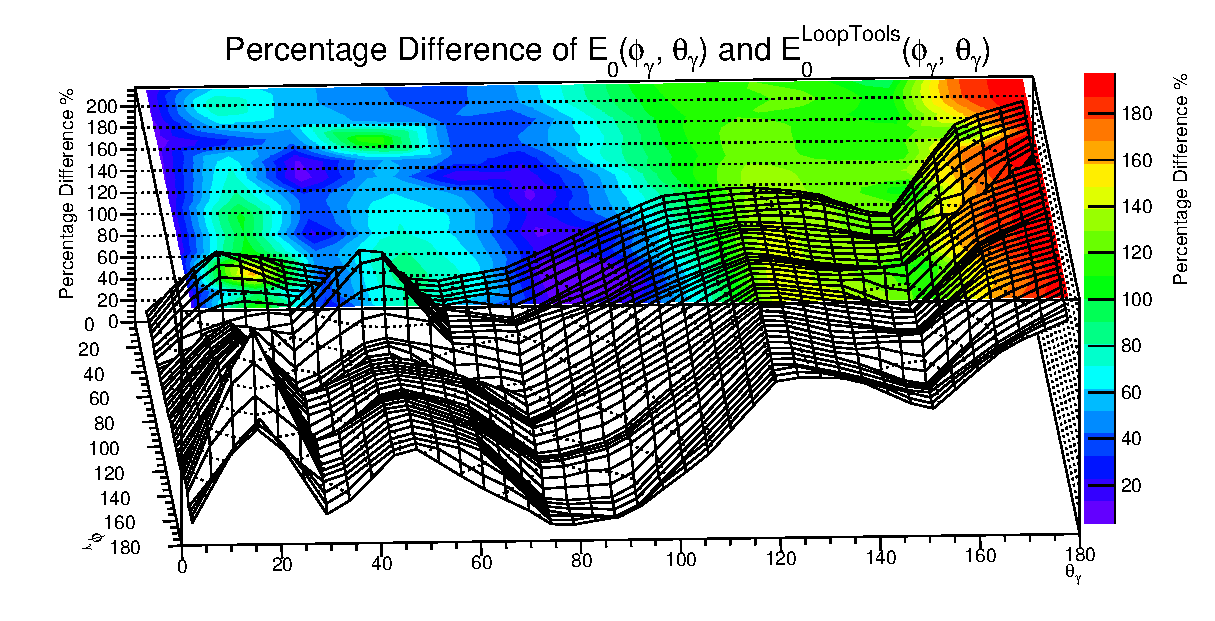
\includegraphics[scale=0.55]{0PD3.eps}
		\caption{ Percentage difference of $E_0(\phi_\gamma,\theta_\gamma)$ and $E_0^{LoopTools}(\phi_\gamma,\theta_\gamma)$ for $\sqrt{s}=500\text{ GeV}$, $M_{V_1}=91\text{ GeV}$, $M_{V_1}=91\text{ GeV}$ and $\theta'_1=0$ }
	\end{center}
\end{figure}

\begin{figure}
	\begin{center}
		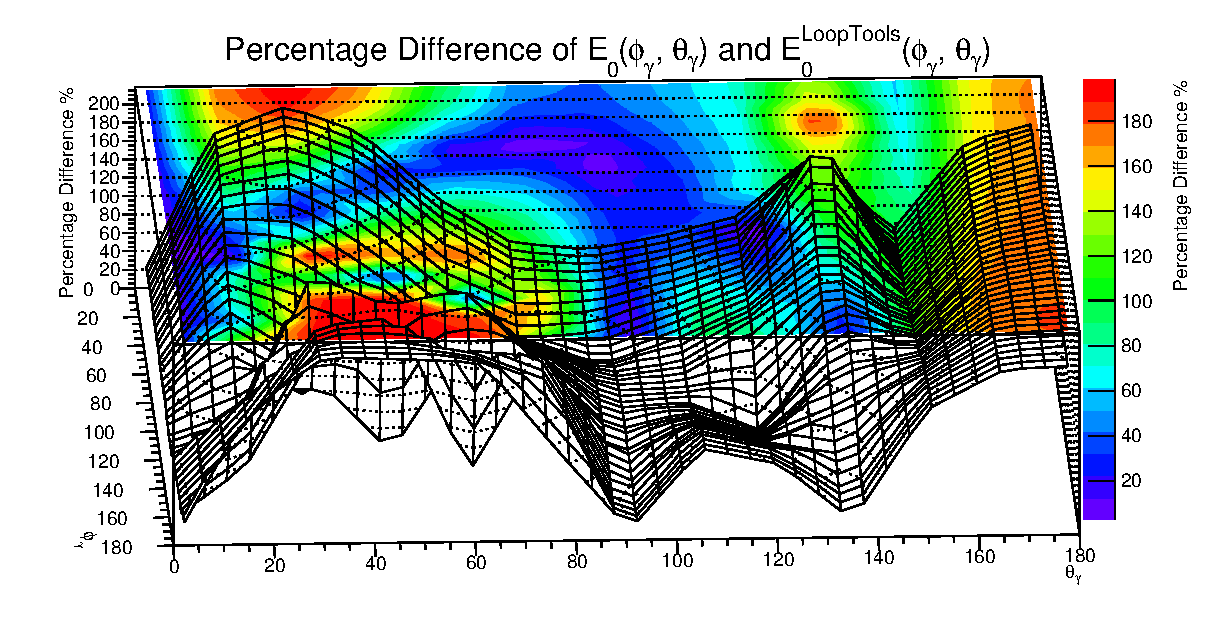
\includegraphics[scale=0.55]{15PD3.eps}
	\caption{ Percentage difference of $E_0(\phi_\gamma,\theta_\gamma)$ and $E_0^{LoopTools}(\phi_\gamma,\theta_\gamma)$ for $\sqrt{s}=500\text{ GeV}$, $M_{V_1}=91\text{ GeV}$, $M_{V_1}=91\text{ GeV}$ and $\theta'_1=15$ }
	\end{center}
\end{figure}

\begin{figure}
	\begin{center}
		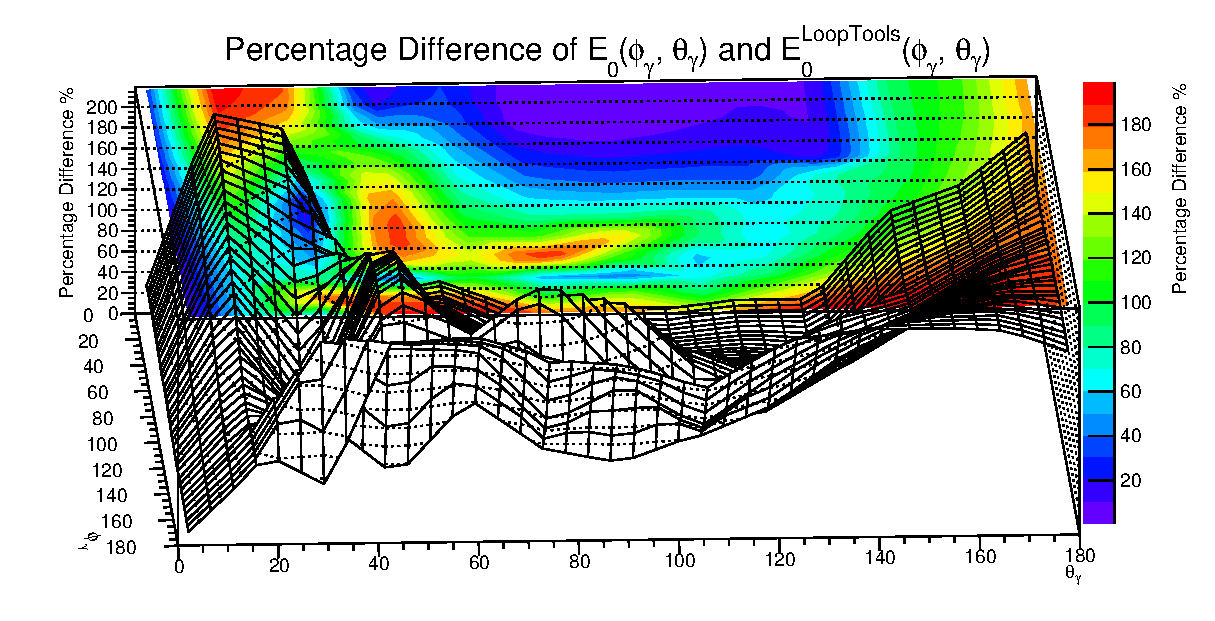
\includegraphics[scale=0.55]{30PD3.eps}\\
	\caption{ Percentage difference of $E_0(\phi_\gamma,\theta_\gamma)$ and $E_0^{LoopTools}(\phi_\gamma,\theta_\gamma)$ for $\sqrt{s}=500\text{ GeV}$, $M_{V_1}=91\text{ GeV}$, $M_{V_1}=91\text{ GeV}$ and $\theta'_1=30$ }
	\end{center}
\end{figure}

\begin{figure}
	\begin{center}
		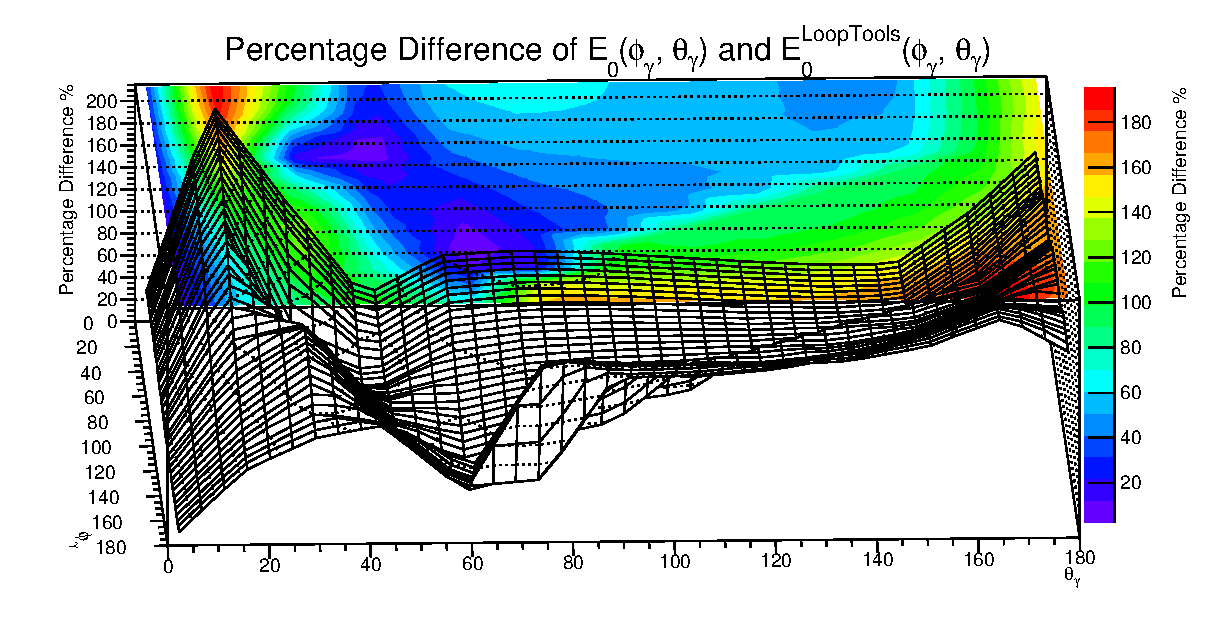
\includegraphics[scale=0.55]{45PD3.eps}\\
	\caption{ Percentage difference of $E_0(\phi_\gamma,\theta_\gamma)$ and $E_0^{LoopTools}(\phi_\gamma,\theta_\gamma)$ for $\sqrt{s}=500\text{ GeV}$, $M_{V_1}=91\text{ GeV}$, $M_{V_1}=91\text{ GeV}$ and $\theta'_1=45$ }
	\end{center}
\end{figure}

\begin{figure}
	\begin{center}
		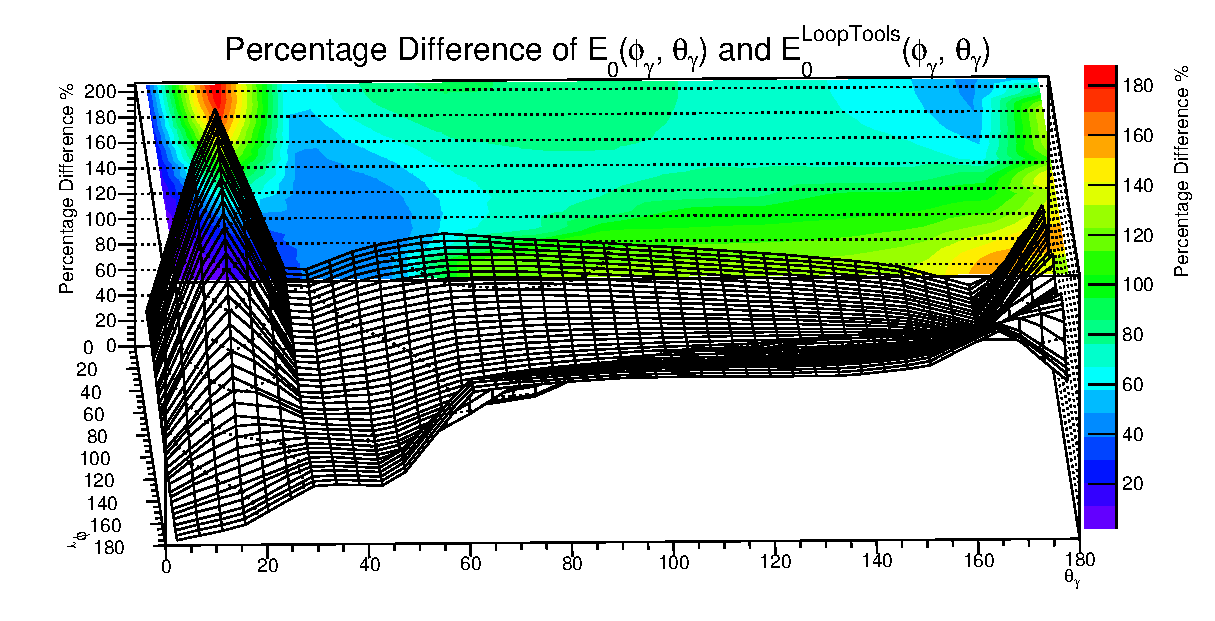
\includegraphics[scale=0.55]{60PD3.eps}\\
	\caption{ Percentage difference of $E_0(\phi_\gamma,\theta_\gamma)$ and $E_0^{LoopTools}(\phi_\gamma,\theta_\gamma)$ for $\sqrt{s}=500\text{ GeV}$, $M_{V_1}=91\text{ GeV}$, $M_{V_1}=91\text{ GeV}$ and $\theta'_1=60$ }
	\end{center}
\end{figure}

\begin{figure}
	\begin{center}
		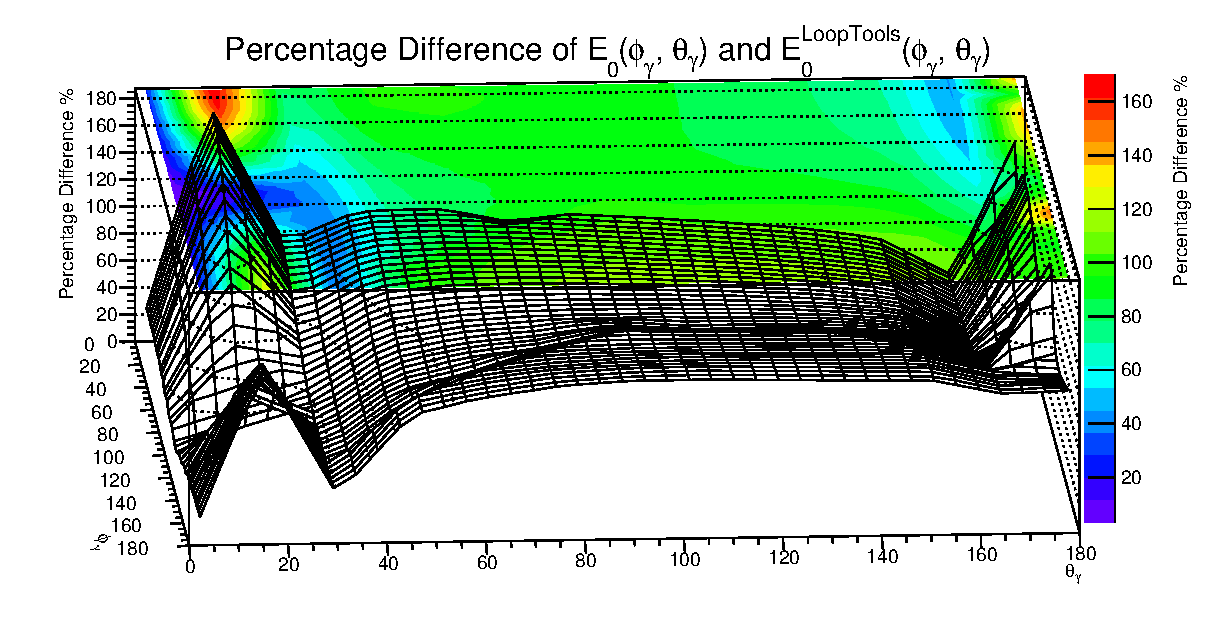
\includegraphics[scale=0.55]{75PD3.eps}\\
	\caption{ Percentage difference of $E_0(\phi_\gamma,\theta_\gamma)$ and $E_0^{LoopTools}(\phi_\gamma,\theta_\gamma)$ for $\sqrt{s}=500\text{ GeV}$, $M_{V_1}=91\text{ GeV}$, $M_{V_1}=91\text{ GeV}$ and $\theta'_1=75$ }
	\end{center}
\end{figure}

\begin{figure}
	\begin{center}
		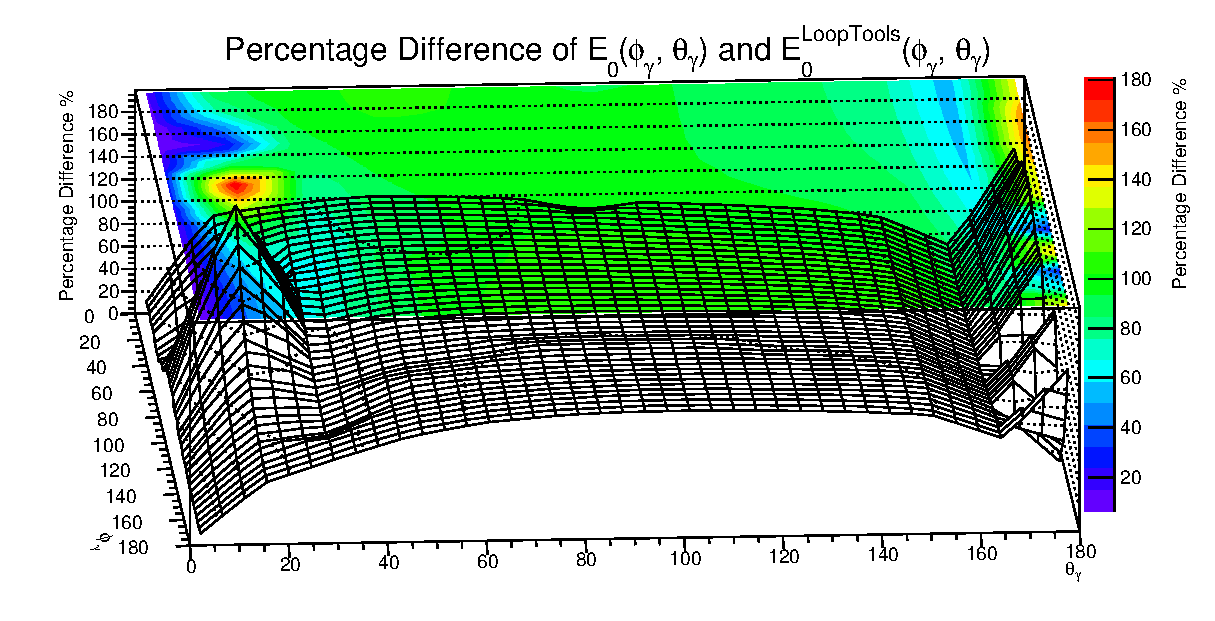
\includegraphics[scale=0.55]{90PD3.eps}\\
		\caption{ Percentage difference of $E_0(\phi_\gamma,\theta_\gamma)$ and $E_0^{LoopTools}(\phi_\gamma,\theta_\gamma)$ for $\sqrt{s}=500\text{ GeV}$, $M_{V_1}=91\text{ GeV}$, $M_{V_1}=91\text{ GeV}$ and $\theta'_1=90$ }
	\end{center}
\end{figure}

\begin{figure}
	\begin{center}
		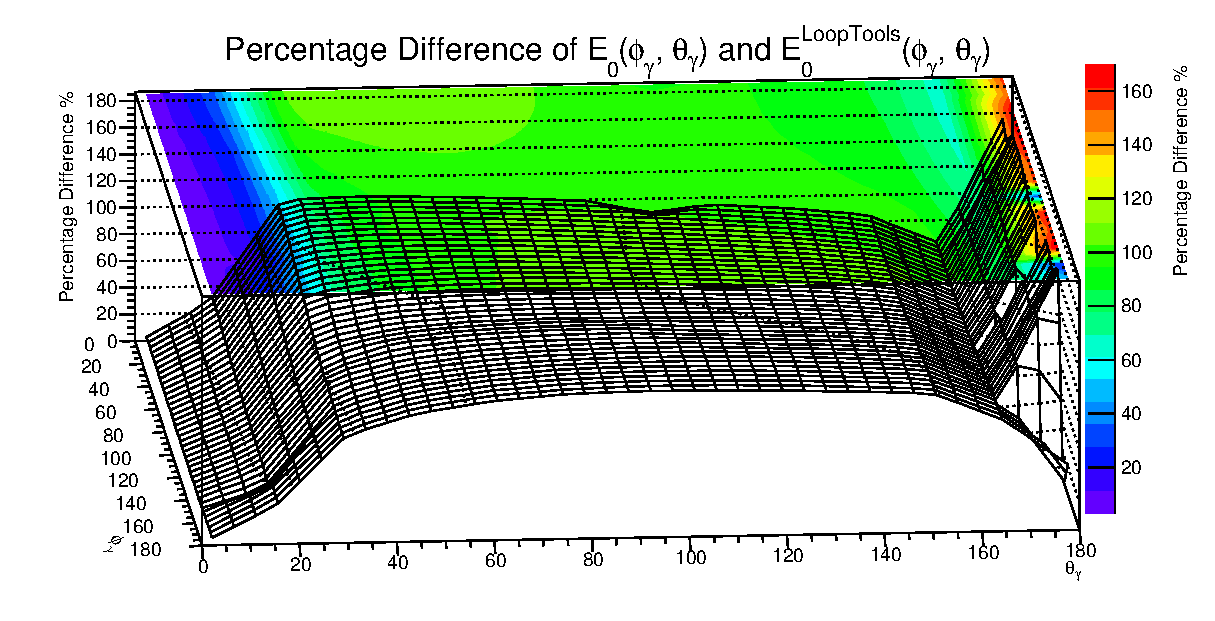
\includegraphics[scale=0.55]{105PD3.eps}\\
		\caption{ Percentage difference of $E_0(\phi_\gamma,\theta_\gamma)$ and $E_0^{LoopTools}(\phi_\gamma,\theta_\gamma)$ for $\sqrt{s}=500\text{ GeV}$, $M_{V_1}=91\text{ GeV}$, $M_{V_1}=91\text{ GeV}$ and $\theta'_1=105$ }
	\end{center}
\end{figure}

\begin{figure}
	\begin{center}
		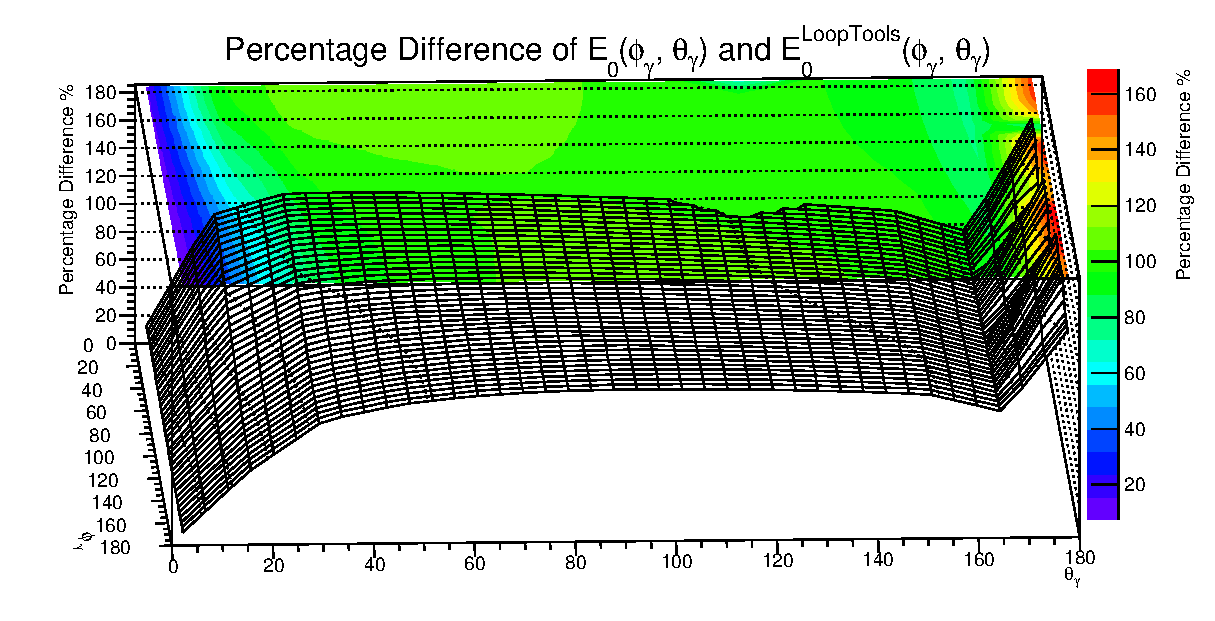
\includegraphics[scale=0.55]{120PD3.eps}\\
		\caption{ Percentage difference of $E_0(\phi_\gamma,\theta_\gamma)$ and $E_0^{LoopTools}(\phi_\gamma,\theta_\gamma)$ for $\sqrt{s}=500\text{ GeV}$, $M_{V_1}=91\text{ GeV}$, $M_{V_1}=91\text{ GeV}$ and $\theta'_1=120$ }
	\end{center}
\end{figure}


\begin{figure}
	\begin{center}
		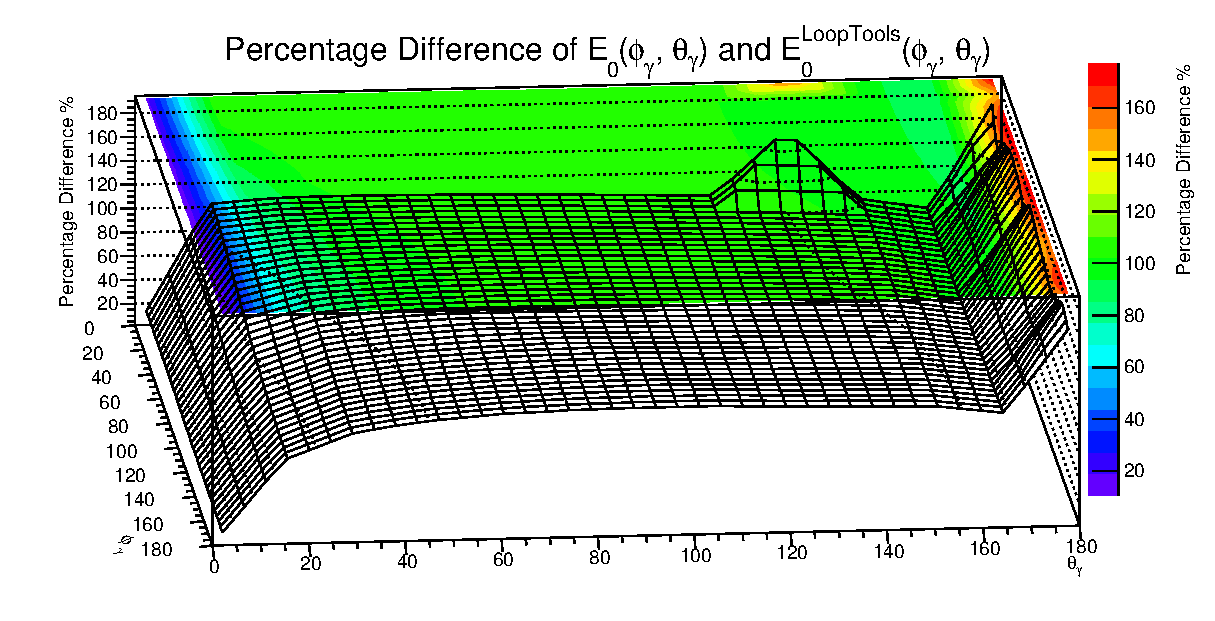
\includegraphics[scale=0.55]{135PD3.eps}\\
		\caption{ Percentage difference of $E_0(\phi_\gamma,\theta_\gamma)$ and $E_0^{LoopTools}(\phi_\gamma,\theta_\gamma)$ for $\sqrt{s}=500\text{ GeV}$, $M_{V_1}=91\text{ GeV}$, $M_{V_1}=91\text{ GeV}$ and $\theta'_1=135$ }
	\end{center}
\end{figure}


\begin{figure}
	\begin{center}
		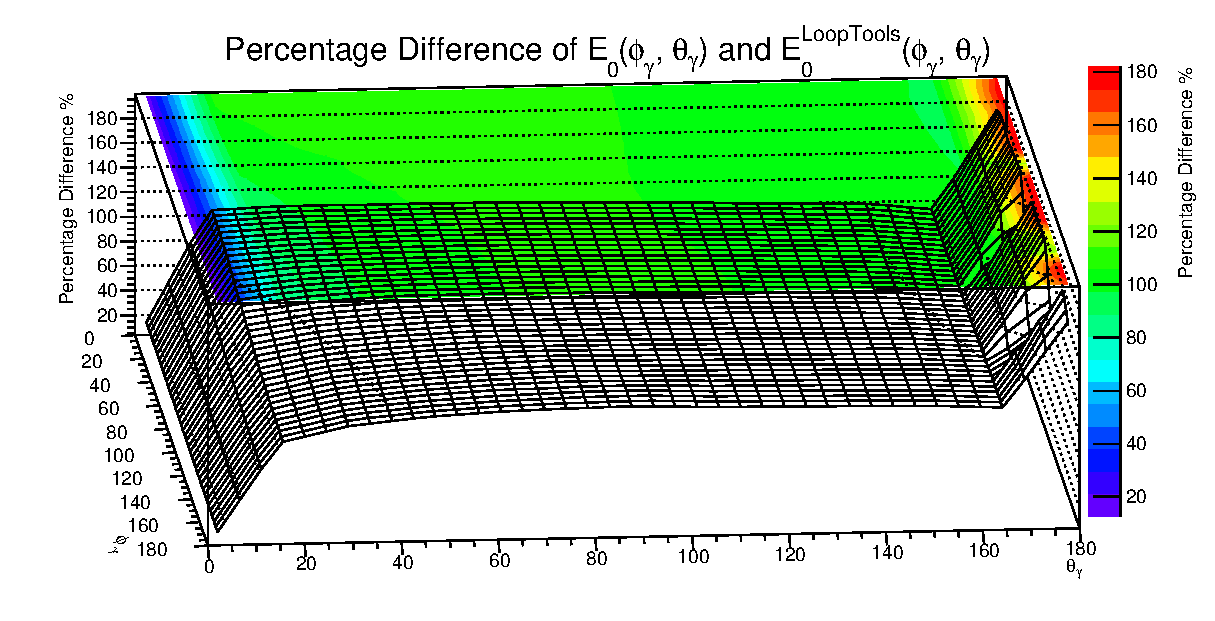
\includegraphics[scale=0.55]{150PD3.eps}\\
		\caption{ Percentage difference of $E_0(\phi_\gamma,\theta_\gamma)$ and $E_0^{LoopTools}(\phi_\gamma,\theta_\gamma)$ for $\sqrt{s}=500\text{ GeV}$, $M_{V_1}=91\text{ GeV}$, $M_{V_1}=91\text{ GeV}$ and $\theta'_1=150$ }
	\end{center}
\end{figure}

\begin{figure}
	\begin{center}
		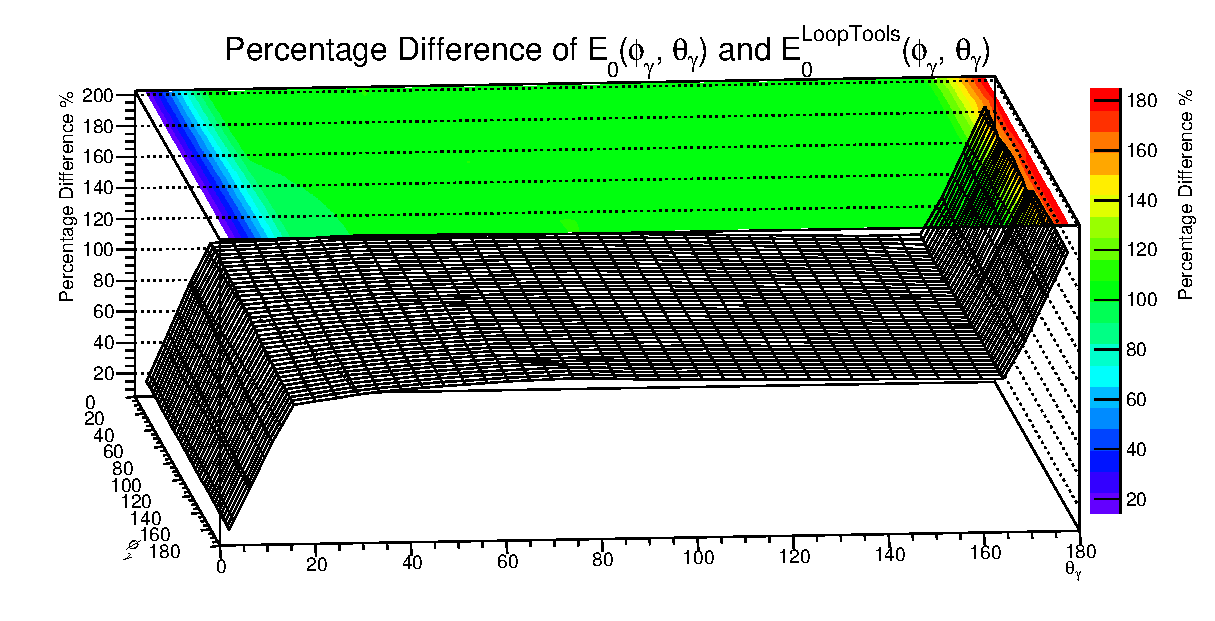
\includegraphics[scale=0.55]{165PD3.eps}\\
		\caption{ Percentage difference of $E_0(\phi_\gamma,\theta_\gamma)$ and $E_0^{LoopTools}(\phi_\gamma,\theta_\gamma)$ for $\sqrt{s}=500\text{ GeV}$, $M_{V_1}=91\text{ GeV}$, $M_{V_1}=91\text{ GeV}$ and $\theta'_1=165$ }
	\end{center}
\end{figure}


\begin{figure}
	\begin{center}
		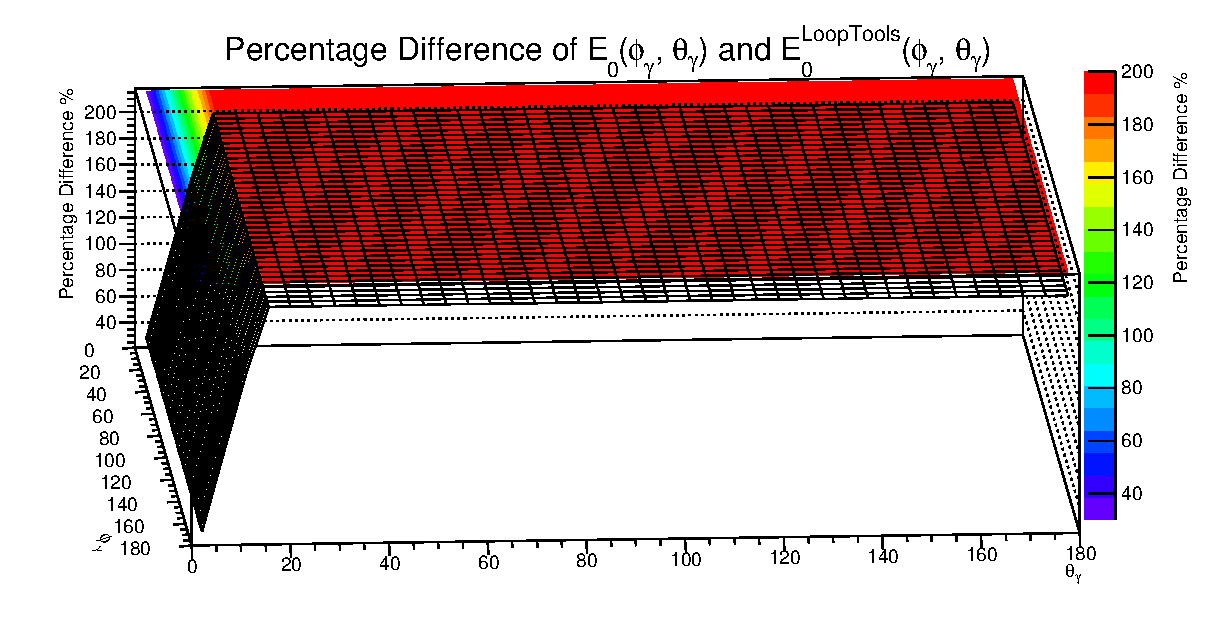
\includegraphics[scale=0.55]{180PD3.eps}\\
		\caption{ Percentage difference of $E_0(\phi_\gamma,\theta_\gamma)$ and $E_0^{LoopTools}(\phi_\gamma,\theta_\gamma)$ for $\sqrt{s}=500\text{ GeV}$, $M_{V_1}=91\text{ GeV}$, $M_{V_1}=91\text{ GeV}$ and $\theta'_1=180$ }
	\end{center}
\end{figure}

As we see, the result from magic spinor product method agrees with that from LoopTools in overall, except several regions. The percentage difference of $E_0(\phi_\gamma,\theta_\gamma)$ and $E_0^{\text{LoopTools}}(\phi_\gamma,\theta_\gamma)$ is insensitive with $\phi_\gamma$, but sensitive with $\theta'_1$. When $\theta'_1>90$, our result mainly fits to that from LoopTool in the region $(0<\phi_\gamma<180,\text{ }0<\theta_\gamma<20)$.
However, when $\theta'_1<75$, our result agrees greatly with that from Looptools.

\chapter{Quantum Chromodynaics}
\section{Introduction to Quantum Chromodynamics}

We now come to the other constituent of the standard model of particle physics, Quantum Chromodynamics (QCD) \cite{Pol,Pol1,GrossWil, GrossWil1, SWQCD, SWQCD1}. Quantum Chromodynamics is a non-Abelian gauge theory of strong interactions. The gauge symmetry of QCD is $SU(3)$ color. The choice of gauge group must rely on three facts: (a) the group must admit complex representations in order to distinguish a quark from antiquark; (b) the group must have completely antisymmtric color singlet to solve the statistical puzzle for the lowest lying baryons of spin $1/2$ and $3/2$; (c) the number of colors for each kind of quarks must agree with the data on the total hadronic $e^+e^-$ annihilation cross section and on the $\pi^0\to2\gamma$. These requirements make the $SU(3)_C$ be the unique choice. The quanta of $SU(3)_C$ is called gluon. Since the $SU(3)_C$ symmetry is unbroken, the gauge boson, gluon, must be massless. Therefore if $A_a^\mu$ denotes the gluon field ($a$ is the color index), $\psi^\alpha_i$ the quark field with flavor index $i$ and color index $\alpha$, the QCD Lagrangian is 
\begin{equation}
\mathcal{L}^\text{classical }=-\frac{1}{4}F_{\mu\nu a}F^{\mu\nu}_a+\bar{\psi}^i( i\slashed D_{ij}-m\delta_{ij}){\psi}^j 
\end{equation}
where
\begin{align}
F^{\mu\nu}_a&=\partial^\mu A^\nu_a-\partial^\nu A^\mu_a+gf_{abc} A^\mu_b A^\nu_c,\\
D^\mu&=\partial^\mu-igA^\mu_aT_{a}.
\end{align} 
Note that last term $gf_{abc}A^\mu_bA^\nu_c$ implies self-interactions of gluons, while there are no such self-interactions in Abelian gauge theory. $T_a$ is the generators of the triplet representation of $SU(3)_C$, following the commutation relations 
\begin{equation}
[T_a, T_b]=if_{abc}T_c,
\end{equation}
where $f_{abc}$ are completely antisymmetric structure constants.  

In order to quantize the theory one needs a gauge fixing term to be added to eq. (5.1). Usually, the gauge fixing term is chosen as follows:
\begin{equation}
\mathcal{L}^\text{gauge fixing}=-\frac{1}{2\alpha}(\partial^\mu A_\mu^a)^2.
\end{equation}
The introduction of such a term requires the addition of the Faddeev-Popov ghost interactions in turn,
\begin{equation}
\mathcal{L}^\text{FP}=(\partial^\mu\chi^{a\ast})D^{ab}_\mu\chi^b,
\end{equation}
where $D^{ab}_\mu$ refer to the adjoint representation of $SU(3)_C$. Here we choose a pair of the ghost fields $\chi^a$ and $\chi^{a\ast}$. It is also possible to choose two real fields $\chi^a_1$ and $\chi^a_2$ instead of $\chi^a$ and $\chi^{a\ast}$. By setting
\begin{equation}
\chi^a=\frac{1}{\sqrt{2}}(\chi^a_1+i\chi^a_2)
\end{equation}
with the Grassmann property
\begin{equation}
(\chi^a_1)^2=(\chi^a_2)^2=0, \quad\text{(no summation on $a$)},
\end{equation}
we can rewrite the Faddeev-Popov ghost term as
\begin{equation}
\mathcal{L}^\text{FP}=i(\partial^\mu\chi_1^{a})D^{ab}_\mu\chi_2^b,
\end{equation}

Therefore, we obtain the complete Lagrangian of the theory
\begin{eqnarray}
\mathcal{L}&=&-\frac{1}{4}(\partial_\mu A^a_\nu-\partial_\nu A^a_\mu)(\partial^\mu A^{a\nu}-\partial^\nu A^{a\mu})-\frac{1}{2\alpha}(\partial^\mu A^a_\mu)^2\nonumber\\
&&+i(\partial^\mu\chi^{a}_1)(\partial_\mu\chi^a_2)+\bar{\psi}^i(i\slashed \partial-m)\psi^i-\frac{g}{2}f^{abc}(\partial_\mu A^a_\nu-\partial_\nu A^a_\mu)A^{b\mu}A^{c\nu}  \nonumber\\
&&-\frac{g^2}{4}f^{abe}{cde}A_\mu^aA_\nu^bA^{c\mu}A^{d\nu}-igf^{abc}(\partial^\mu\chi^{a}_1)\chi^b_2 A_\mu^c+g\bar{\psi}^iT_{ij}^a\gamma^\mu\psi^j A^a_\mu.\nonumber\\
\end{eqnarray}
Accordingly we obtain Feynman rules for the Lagrangian of quantum chromodynamics (see Appendix B). This theory is renormalizable \cite{AbersLee}. 

We are here using the couterterm approach to realize renormalization again with similar procedure describle in the Section (2.2). We redefine the fields $A_\mu^a$, $\chi^a_1$, $\chi_2^a$ and $\psi$ by
\begin{equation}
A_\mu^a=Z_3^\frac{1}{2} A_{\mu R}^a,\quad \chi^a_{1,2}=\widetilde{Z}^\frac{1}{2}_3\chi^a_{1,2R} ,\quad\psi=Z^\frac{1}{2}_2\psi_R,
\end{equation}
and the parameters $g$, $\alpha$ and $m$ by
\begin{equation}
g=Z_g g_R,\quad\alpha=Z_3\alpha_R,\quad m=Z_m m_R,
\end{equation}
where the constants $Z_3$, $\widetilde{Z}_3$ and $Z_2$ denote the gauge field, ghost field and quark field renormalization constants, respectively, while the constants $Z_g$ and $Z_m$ car called the coupling-constant and mass renormalization constants. 

Inserting eqs. (5.11) and (5.12) into eq. (5.10), we have 
\begin{equation}
\mathcal{L}=\mathcal{L}^\text{R}+\mathcal{L}^\text{C}
\end{equation}
where the renormalized Lagrangian $\mathcal{L}^\text{R}$ is precisely equal to $\mathcal{L}$ if the quantities $\{A^a_\mu,\chi^a_{1,2},\psi,g,\alpha\}$ are replaced by the renormalized ones, $\{A^a_{\mu R},\chi^a_{1,2R},\psi_R,g_R,\alpha_R\}$. The counterterm Lagrangian $\mathcal{L}^\text{C}$ is given by 
\begin{eqnarray}
\mathcal{L}^\text{C}&=&(Z_3-1)\frac{1}{2}A_R^{a\mu}\delta_{ab}(g_{\mu\nu}\partial^2-\partial_\mu\partial_\nu)A_R^{b\nu}+(\widetilde{Z}_3-1)\chi_{1R}^a\delta_{ab}(-i\partial^2)\chi_{2R}^b\nonumber\\
&&+(Z_2-1)\bar{\psi}^i_R(i\slashed\partial-m_R)\psi_R^i-Z_2(Z_m-1)m_R\bar{\psi}^i_R\psi^i_R\nonumber\\
&&-(Z_1-1)\frac{1}{2}g_Rf^{abc}(\partial_\mu A^a_{\nu R}-\partial_\nu A^a_{\mu R})A_R^{\mu b}A_R^{\nu c}\nonumber\\
&&-(Z_4-1)\frac{1}{4}g^2_Rf^{abe}f^{cde}A^a_{\mu R}A^b_{\nu R}A_R^{c\mu}A_R^{d\nu}\nonumber\\
&&-(\widetilde{Z}_1-1)ig_Rf^{abc}(\partial^\mu\chi_{1R}^a)\chi_{2R}^bA^c_{\mu R}\nonumber\\
&&+(Z_{1F}-1)g_R\bar{\psi}^iT^a_{ij}\gamma^\mu\psi_R^jA^a_{\mu R},
\end{eqnarray}
where $Z_1$, $Z_4$, $\widetilde{Z}_1$ and $Z_{1F}$ are defined as follows:
\begin{eqnarray}
&Z_1\equiv Z_gZ_3^\frac{3}{2}, & Z_4\equiv Z^2_gZ^2_3,\nonumber\\
&\widetilde{Z}_1\equiv Z_g\widetilde{Z}_3Z_3^\frac{1}{2}, & Z_{1F}\equiv Z_gZ_2Z_3^\frac{1}{2}.
\end{eqnarray}
From this counterterm term we obtain the corresponding Feynman rules (see Appendix B).

The gauge nature of the theory implies the Slavnov-Taylor identity \cite{Tay71,Sla73}, 
\begin{equation}
\frac{Z_1}{Z_3}=\frac{\widetilde{Z}_1}{\widetilde{Z}_3}=\frac{Z_{1F}}{Z_2}=\frac{Z_4}{Z_1}.
\end{equation} 
The Slavnov-Taylor identity ensures the universality of the renormalized coupling constant $g_R$.

By the power counting analysis in the case of QCD, we have seven amplitdues which possess overall divergences. The Feynman diagrams with non-negative superficial degree of divergence in QCD are outlined below:

Note that the superficial degrees of divergence $d$ for the self-energy part for the gluon, Faddeev-Popov ghost and quark and three-gluon vertex are 2, 1, 1 and 1, respectively, but the actual degrees of divergences of these amplitudes are all logarithmic due to the gauge invariance. Next, we present one-loop contributions to the seven superficially divergent amplitudes \cite{Muta,Cel79,Pas80}:



(\romannumeral 1) The gluon self-energy $\Pi^{ab}_{\mu\nu}(k)$ is
\begin{equation}
\Pi^{ab}_{\mu\nu}(k)=\delta_{ab}(k_\mu k_\nu-k^2g_\mu\nu)\Pi(k^2),
\end{equation}
\begin{equation}
\Pi(k^2)=\frac{g^2_R}{(4\pi)^2}\biggl[\frac{4}{3}T_RN_f-\frac{1}{2}C_G\left(\frac{13}{3}-\alpha_R \right) \biggr]\frac{1}{\epsilon}+Z_3-1+\text{ finite terms,}
\end{equation}
\def\GLSE1{
	\raisebox{-38.2pt}{
		\begin{axopicture}(100,60)
			\Gluon(5,37)(30,37){3}{3}
			\Gluon(70,37)(95,37){3}{3}
			\GCirc(50,37){20}{0.67}
		\end{axopicture}
		
	}
}	

\def\gGLSE{
	\raisebox{-38.2pt}{
		\begin{axopicture}(100,60)
			\Gluon(5,37)(30,37){3}{3}
			\Gluon(70,37)(95,37){3}{3}
			\GluonArc(50,37)(20,0,360){3}{10}
		\end{axopicture}
		
	}
}	


\def\ggGLSE{
	\raisebox{-38.2pt}{
		\begin{axopicture}(100,60)
			\Gluon(5,37)(50,37){3}{4}
			\Gluon(50,37)(95,37){3}{4}
			\GluonArc(50,60)(20,0,180){3}{5}
			\GluonArc(50,60)(20,180,360){3}{5}
		\end{axopicture}
		
	}
}		


\def\gggGLSE{
	\raisebox{-38.2pt}{
		\begin{axopicture}(100,60)
			\Gluon(5,37)(30,37){3}{3}
			\Gluon(70,37)(95,37){3}{3}
			\Arc[arrow,dash,clockwise](50,37)(20,0,180)
			\Arc[arrow,dash,clockwise](50,37)(20,180,360)
		\end{axopicture}
		
	}
}	

\def\ggggGLSE{
	\raisebox{-38.2pt}{
		\begin{axopicture}(100,60)
			\Gluon(5,37)(30,37){3}{3}
			\Gluon(70,37)(95,37){3}{3}
			\Arc[arrow,clockwise](50,37)(20,0,180)
			\Arc[arrow,clockwise](50,37)(20,180,360)
		\end{axopicture}
		
	}
}		

\def\cGLSE1{
	\raisebox{-38.2pt}{
		\begin{axopicture}(100,60)
			\Gluon(5,37)(95,37){3}{10}
			\GCirc(50,37){5}{1}
			\Line(46.464,40.535)(53.535,33.464)
			\Line(53.535,40.535)(46.464,33.464)
		\end{axopicture}
		
	}
}	

\begin{eqnarray}
\GLSE1&=&\gGLSE+ \ggGLSE\nonumber
\\&&+\gggGLSE+\ggggGLSE\nonumber\\
&&+\cGLSE1\nonumber
\end{eqnarray}
where $\epsilon=(4-D)/2$. In Eq. (5.18) we have taken $N_f$ flavors of quarks into account, and $T_R$ and $C_G$ are the constants defined by
\begin{align}
tr[T_aT_b]&=\delta_{ab}T_R,\nonumber\\
f_{acd}f_{bcd}&=\delta_{ab}C_G.
\end{align} 
Here we have $T_R=\frac{1}{2}$ and $C_G=3$ for $SU(3)_C$. Note that the one-loop contribution to the gluon self-energy satisfies the Ward-Takahashi identities,
\begin{equation}
k^\mu\Pi_{\mu\nu}^{ab}(k)=0,
\end{equation}
which is a natural consequence of gauge invariance. Due to this constraint the amplitude $\Pi_{\mu\nu}^{ab}$ must have the factor
$k_\mu k_\nu-k^2g_{\mu\nu}$ and the degree of divergence for $\Pi_{\mu\nu}^{ab}(k)$ is lowered by 2 units. This structure of $\Pi_{\mu\nu}^{ab}(k)$ forbids a mass terms and so there is no mass renormalization. Therefore the gluon remains massless under the radiative corrections. In th MS scheme \cite{MS} the gauge field renormalization constant $Z_3$ is given by
\begin{equation}
Z_3=1-\frac{g^2_R}{(4\pi)^2}\biggl[\frac{4}{3}T_RN_f-\frac{1}{2}C_G\left(\frac{13}{3}-\alpha_R \right) \biggr]\frac{1}{\epsilon}+O(g^4_R).
\end{equation}

(\romannumeral 2) The Faddeev-Popov ghost self-energy $\widetilde{\Pi}^{ab}(k)$ is
\begin{equation}
\widetilde{\Pi}^{ab}(k)\delta_{ab}\bigg[ -\frac{g^2_R}{(4\pi)^2}C_G\frac{3-\alpha_R}{4}\frac{1}{\epsilon}+\widetilde{Z}_3-1 \bigg]+\text{ finite terms.}
\end{equation} 

\def\FSE{
	\raisebox{-38.2pt}{
		\begin{axopicture}(100,60)
			\Line[arrow,dash](30,37)(5,37)
			\Line[arrow,dash](95,37)(70,37)
			\GCirc(50,37){20}{0.67}
		\end{axopicture}
		
	}
}	


\def\FSEf{
	\raisebox{-38.2pt}{
		\begin{axopicture}(100,60)
			\Line[arrow,dash](95,37)(5,37)
			\GluonArc(50,37)(20,0,180){3}{8}
		\end{axopicture}
		
	}
}	


\def\cFSE{
	\raisebox{-38.2pt}{
		\begin{axopicture}(100,60)
			\Line[arrow,dash](46.464,37)(5,37)
			\Line[arrow,dash](95,37)(53.535,37)
			\GCirc(50,37){5}{1}
			\Line(46.464,40.535)(53.535,33.464)
			\Line(53.535,40.535)(46.464,33.464)
		\end{axopicture}
		
	}
}	

\begin{eqnarray}
\FSE= \FSEf+\cFSE\nonumber
\end{eqnarray}
Note that the divergent part above is proportional to $k^2$ and thus there is no mass renormalization. So the Faddeev-Popov ghost self-energy remain massless after radiative corrections, too. The ghost field renormalization constant $\widetilde{Z}$ in the MS scheme is given by
\begin{equation}
\widetilde{Z}_3=1+\frac{g^2_R}{(4\pi)^2}C_G\frac{3-\alpha_R}{4}\frac{1}{\epsilon}+O(g^4_R).
\end{equation}

(\romannumeral 3) The quark self-energy $\Sigma^{ij}(p)$ is 
\begin{eqnarray}
\Sigma^{ij}(p)&=&\delta_{ij}[(Am_R-B\slashed p)-(Z_2Z_m-1)m_R+(Z_2-1)\slashed p]+\text{ finite terms,}\nonumber\\
A&=&-\frac{g^2_R}{(4\pi)^2}C_F(3+\alpha_R)\frac{1}{\epsilon}+O(g^4_R),\nonumber\\
B&=&-\frac{g^2_R}{(4\pi)^2}C_F\alpha_R\frac{1}{\epsilon}+O(g^4_R).
\end{eqnarray}
\def\QSE{
	\raisebox{-38.2pt}{
		\begin{axopicture}(100,60)
			\Line[arrow](30,37)(5,37)
			\Line[arrow](95,37)(70,37)
			\GCirc(50,37){20}{0.67}
		\end{axopicture}
		
	}
}	


\def\QSEf{
	\raisebox{-38.2pt}{
		\begin{axopicture}(100,60)
			\Line[arrow](95,37)(5,37)
			\GluonArc(50,37)(20,0,180){3}{8}
		\end{axopicture}
		
	}
}	


\def\cQSE{
	\raisebox{-38.2pt}{
		\begin{axopicture}(100,60)
			\Line[arrow](46.464,37)(5,37)
			\Line[arrow](95,37)(53.535,37)
			\GCirc(50,37){5}{1}
			\Line(46.464,40.535)(53.535,33.464)
			\Line(53.535,40.535)(46.464,33.464)
		\end{axopicture}
		
	}
}	



\begin{eqnarray}
\QSE= \QSEf+\cQSE\nonumber
\end{eqnarray}	
As we see, the divergence in the quark self-energy consists of two kinds, the mass type $Am_R$ and the kinetic energy type $-B\slashed p$. Then the mass and quark-field renormalization constants in the MS scheme are determined by
\begin{eqnarray}
Z_m&=&1-\frac{g^2_R}{(4\pi)^2}C_F(3+\alpha_R)\frac{1}{\epsilon}+\frac{g^2_R}{(4\pi)^2}C_F\alpha_R\frac{1}{\epsilon}+O(g^4_R),\nonumber\\
Z_2&=&1-\frac{g^2_R}{(4\pi)^2}C_F\alpha_R\frac{1}{\epsilon}+O(g^4_R).
\end{eqnarray}

(\romannumeral 4) The three-gluon vertex $\Lambda^{abc}_{\mu\nu\lambda}(K_1,k_2,k_3)$ is given by
\begin{eqnarray}
\Lambda^{abc}_{\mu\nu\lambda}(K_1,k_2,k_3)&=&-ig_Rf^{abc}V_{\mu\nu\lambda}(k_1,k_2,k_3)\biggl\{ \frac{g^2_R}{(4\pi)^2}\bigg[ C_G\left( -\frac{17}{12}+\frac{3\alpha_R}{4}\right)\nonumber\\
&&+\frac{4}{3}T_RN_f \bigg]\frac{1}{\epsilon}+Z_1-1 \biggr\}+\text{ finite terms,}
\end{eqnarray}

\def\GGG{
	\raisebox{-38.2pt}{
		\begin{axopicture}(100,100)
			\Gluon(5,37)(30,37){3}{3}
			\Gluon(70,37)(95,37){3}{3}
			\Gluon(50,57)(50,77){3}{3}
			\GCirc(50,37){20}{0.67}
		\end{axopicture}
		
	}
}	


\def\gGGG{
	\raisebox{-38.2pt}{
		\begin{axopicture}(100,100)
			\Gluon(5,37)(35,37){3}{3}
			\Gluon(65,37)(95,37){3}{3}
			\Gluon(35,37)(65,37){3}{3}
			\Gluon(50,57)(50,77){3}{3}
			\Gluon(35,37)(50,57){3}{3}
			\Gluon(65,37)(50,57){3}{3}
		\end{axopicture}
		
	}
}	

\def\gGGG{
	\raisebox{-38.2pt}{
		\begin{axopicture}(100,100)
			\Gluon(5,37)(35,37){3}{3}
			\Gluon(65,37)(95,37){3}{3}
			\Gluon(35,37)(65,37){3}{3}
			\Gluon(50,57)(50,77){3}{3}
			\Gluon(35,37)(50,57){3}{3}
			\Gluon(65,37)(50,57){3}{3}
		\end{axopicture}
		
	}
}	


\def\ggGGG{
	\raisebox{-38.2pt}{
		\begin{axopicture}(100,100)
			\Gluon(5,37)(50,37){3}{3}
			\Gluon(50,37)(95,37){3}{3}
			\Gluon(50,77)(50,97){3}{3}
			\GluonArc(50,57)(15,0,360){3}{10}
		\end{axopicture}
		
	}
}	

\def\gggGGG{
	\raisebox{-38.2pt}{
		\begin{axopicture}(100,100)
			\Gluon(5,37)(35,37){3}{3}
			\Gluon(65,37)(95,37){3}{3}
			\Gluon(50,57)(50,77){3}{3}
			\Line[arrow,dash](65,37)(35,37)
			\Line[arrow,dash](35,37)(50,57)
			\Line[arrow,dash](50,57)(65,37)
		\end{axopicture}
		
	}
}	

\def\ggggGGG{
	\raisebox{-38.2pt}{
		\begin{axopicture}(100,100)
			\Gluon(5,37)(35,37){3}{3}
			\Gluon(65,37)(95,37){3}{3}
			\Gluon(50,57)(50,77){3}{3}
			\Line[arrow](65,37)(35,37)
			\Line[arrow](35,37)(50,57)
		\Line[arrow](50,57)(65,37)
	\end{axopicture}
	
}
}	


\def\cGGG{
\raisebox{-38.2pt}{
	\begin{axopicture}(100,60)
		\Gluon(5,37)(95,37){3}{10}
		\Gluon(50,37)(50,77){3}{5}
		\GCirc(50,37){5}{1}
		\Line(46.464,40.535)(53.535,33.464)
		\Line(53.535,40.535)(46.464,33.464)
	\end{axopicture}
	
}
}

\begin{eqnarray}
\GGG&=&\gGGG+\ggGGG \nonumber\\
&&+\gggGGG+\ggggGGG\nonumber\\
&&+\text{ permutations } +\cGGG\nonumber
\end{eqnarray}
where
\begin{equation}
V_{\mu\nu\lambda}(k_1,k_2,k_3)=(k_1-k_2)_\lambda g_{\mu\nu}+(k_2-k_3)_\mu g_{\nu\lambda}+(k_3-k_1)_\nu g_{\mu\lambda}.
\end{equation}
The three-gluon vertex renormalization constant $Z_1$ in the MS scheme is
\begin{equation}
Z_1=1-\frac{g^2_R}{(4\pi)^2}\bigg[ C_G\left( -\frac{17}{12}+\frac{3\alpha_R}{4}\right)+\frac{4}{3}T_RN_f \bigg]\frac{1}{\epsilon}+O(g^4_R).
\end{equation}

(\romannumeral 5) The ghost-gluon vertex $\widetilde{\Lambda}^{abc}_\mu(k,p,p')$ has the express
\begin{equation}
\widetilde{\Lambda}^{abc}_\mu(k,p,p')=-ig_Rf^{abc}p_\mu\biggl[ \frac{g^2_R}{(4\pi)^2}C_G\frac{\alpha_R}{2}\frac{1}{\epsilon}+\widetilde{Z}_1-1 \biggr]+\text{ finite terms,}
\end{equation}

\def\FGV{
	\raisebox{-38.2pt}{
		\begin{axopicture}(100,100)
			\Line[arrow,dash](30,37)(5,37)
			\Line[arrow,dash](95,37)(70,37)
			\Gluon(50,57)(50,77){3}{3}
			\GCirc(50,37){20}{0.67}
		\end{axopicture}
		
	}
}	


\def\fFGV{
	\raisebox{-38.2pt}{
		\begin{axopicture}(100,100)
			\Line[arrow,dash](95,37)(70,37)
			\Line[arrow,dash](30,37)(5,37)
			\Line[dash](30,37)(70,37)
			\Gluon(50,37)(50,77){3}{3}
			\GluonArc(50,37)(20,180,360){3}{6}
		\end{axopicture}
		
	}
}		

\def\ffFGV{
	\raisebox{-38.2pt}{
		\begin{axopicture}(100,100)
			\Line[arrow,dash](35,37)(5,37)
			\Line[arrow,dash](95,37)(65,37)
			\Line[dash](65,37)(35,37)
			\Gluon(50,57)(50,77){3}{3}
			\Gluon(35,37)(50,57){3}{3}
			\Gluon(65,37)(50,57){3}{3}
		\end{axopicture}
		
	}
}	

\def\cFGV{
	\raisebox{-38.2pt}{
		\begin{axopicture}(100,90)
			\Line[arrow,dash](50,37)(5,37)
			\Line[arrow,dash](95,37)(50,37)
			\Gluon(50,37)(50,77){3}{5}
			\GCirc(50,37){5}{1}
			\Line(46.464,40.535)(53.535,33.464)
			\Line(53.535,40.535)(46.464,33.464)
		\end{axopicture}
		
	}
}	

\begin{eqnarray}
\FGV&=&\fFGV+\ffFGV\nonumber\\
&&+\cFGV\nonumber
\end{eqnarray}
where the momentum $p_\mu$ denotes the ghost-line which carries the ghost number flowing out of the vertex. The ghost-gluon vertex renormalization constant $\widetilde{Z}_1$ reads in the MS scheme
\begin{equation}
\widetilde{Z}_1=1-\frac{g^2_R}{(4\pi)^2}C_G\frac{\alpha_R}{2}\frac{1}{\epsilon}+O(g^4_R).
\end{equation}

(\romannumeral 6) The quark-gluon vertex $\Lambda^{aij}_{F\mu}(k,p,p')$ is 
\begin{eqnarray}
\Lambda^{aij}_{F\mu}(k,p,p')&=&g_R\gamma_\mu T^a_{ij}\biggl[ \frac{g^2_R}{(4\pi)^2}\left( \frac{3+\alpha_R}{4}C_G+\alpha_RC_F \right)\frac{1}{\epsilon}+Z_{1F}-1 \biggr]\nonumber\\
&&+\text{ finite terms.}
\end{eqnarray}

\def\QGV{
	\raisebox{-38.2pt}{
		\begin{axopicture}(100,100)
			\Line[arrow](30,37)(5,37)
			\Line[arrow](95,37)(70,37)
			\Gluon(50,57)(50,77){3}{3}
			\GCirc(50,37){20}{0.67}
		\end{axopicture}
		
	}
}	


\def\fQGV{
	\raisebox{-38.2pt}{
		\begin{axopicture}(100,100)
			\Line[arrow](95,37)(70,37)
			\Line[arrow](30,37)(5,37)
			\Line(30,37)(70,37)
			\Gluon(50,37)(50,77){3}{3}
			\GluonArc(50,37)(20,180,360){3}{6}
		\end{axopicture}
		
	}
}		

\def\ffQGV{
	\raisebox{-38.2pt}{
		\begin{axopicture}(100,100)
			\Line[arrow](35,37)(5,37)
			\Line[arrow](95,37)(65,37)
			\Line(65,37)(35,37)
			\Gluon(50,57)(50,77){3}{3}
			\Gluon(35,37)(50,57){3}{3}
			\Gluon(65,37)(50,57){3}{3}
		\end{axopicture}
		
	}
}	

\def\cQGV{
	\raisebox{-38.2pt}{
		\begin{axopicture}(100,90)
			\Line[arrow](50,37)(5,37)
			\Line[arrow](95,37)(50,37)
			\Gluon(50,37)(50,77){3}{5}
			\GCirc(50,37){5}{1}
			\Line(46.464,40.535)(53.535,33.464)
			\Line(53.535,40.535)(46.464,33.464)
		\end{axopicture}
		
	}
}	

\begin{eqnarray}
\QGV&=&\fQGV+\ffQGV\nonumber\\
&&+\cQGV\nonumber
\end{eqnarray}
The quark-gluon vertex renormalization constant $Z_{1F}$ is given by
\begin{equation}
Z_{1F}=1-\frac{g^2_R}{(4\pi)^2}\left( \frac{3+\alpha_R}{4}C_G+\alpha_RC_F \right)\frac{1}{\epsilon}+O(g^4_R).
\end{equation}

(\romannumeral 7) The four-gluon vertex $\Lambda^{a_1\cdots a_4}_{\mu_1\cdots \mu_4}(k_1,k_2,k_3,k_4)$ is 
\begin{eqnarray}
&&\Lambda^{a_1\cdots a_4}_{\mu_1\cdots \mu_4}(k_1,k_2,k_3,k_4)\nonumber\\
&&=-g^2_RW^{a_1\cdots a_4}_{\mu_1\cdots\mu_4} \biggl\{ \frac{g^2_R}{(4\pi)^2}\biggl[ \left( -\frac{2}{3}+\alpha_R \right)C_G+\frac{4}{3}T_RN_f \biggr]\frac{1}{\epsilon}+Z_4-1 \biggr\}\nonumber\\
&&+\text{ finite terms,}
\end{eqnarray}

\def\Gf{
	\raisebox{-45.2pt}{
		\begin{axopicture}(100,100)
			\Gluon(5,5)(95,95){3}{10}
			\Gluon(5,95)(95,5){3}{10}
			\GCirc(50,50){20}{0.65}
			
			
		\end{axopicture}
		
	}
}	

\def\Gfg{
	\raisebox{-45.2pt}{
		\begin{axopicture}(100,100)
			\Gluon(5,5)(35.858,35.858){3}{5}
			\Gluon(64.142,64.142)(95,95){3}{5}
			\Gluon(5,95)(35.858,64.142){3}{5}
			\Gluon(64.142,35.858)(95,5){3}{5}
			\GluonArc(50,50)(20,0,360){3}{10}
		\end{axopicture}
		
	}
}	

\def\Gfgg{
	\raisebox{-45.2pt}{
		\begin{axopicture}(100,100)
			\Gluon(5,5)(35.858,35.858){3}{5}
			\Gluon(5,95)(35.858,64.142){3}{5}
			\GluonArc(50,50)(20,0,360){3}{11}
			\Gluon(70,50)(95,85){3}{5}
			\Gluon(70,50)(95,25){3}{5}
		\end{axopicture}
		
	}
}	

\def\Gfggg{
	\raisebox{-45.2pt}{
		\begin{axopicture}(100,100)
			\Gluon(30,50)(5,85){3}{5}
			\Gluon(30,50)(5,25){3}{5}
			\GluonArc(50,50)(20,0,360){3}{11}
			\Gluon(70,50)(95,85){3}{5}
			\Gluon(70,50)(95,25){3}{5}
		\end{axopicture}
		
	}
}	


\def\GfFP{
	\raisebox{-45.2pt}{
		\begin{axopicture}(100,100)
			\Gluon(5,5)(35.858,35.858){3}{5}
			\Gluon(64.142,64.142)(95,95){3}{5}
			\Gluon(5,95)(35.858,64.142){3}{5}
			\Gluon(64.142,35.858)(95,5){3}{5}
			\DashArc(50,50)(20,0,360){4}
		\end{axopicture}
		
	}
}	

\def\GfFF{
	\raisebox{-45.2pt}{
		\begin{axopicture}(100,100)
			\Gluon(5,5)(35.858,35.858){3}{5}
			\Gluon(64.142,64.142)(95,95){3}{5}
			\Gluon(5,95)(35.858,64.142){3}{5}
			\Gluon(64.142,35.858)(95,5){3}{5}
			\Arc(50,50)(20,0,360)
		\end{axopicture}
		
	}
}	

\def\cGf{
	\raisebox{-45.2pt}{
		\begin{axopicture}(100,100)
			\Gluon(5,5)(95,95){3}{9}
			\Gluon(5,95)(95,5){3}{9}
			\GCirc(50,50){5}{1}
			\Line(46.464,53.535)(53.535,46.464)
			\Line(53.535,53.535)(46.464,46.464)
			
			
		\end{axopicture}
		
	}
}



\begin{eqnarray}
\Gf&=&\Gfg+\Gfgg\nonumber]]\nonumber\\
&&+\Gfggg+\GfFP\nonumber\\
&&+\GfFF+\text{ permutations }\nonumber\\
&&+\cGf\nonumber
\end{eqnarray}
where
\begin{eqnarray}
W^{a_1\cdots a_4}_{\mu_1\cdots\mu_4}&=&(f^{13,24}-f^{14,32})g_{\mu_1\mu_2}g_{\mu_3\mu_4}+(f^{12,34}-f^{14,23})g_{\mu_1\mu_3}g_{\mu_2\mu_4}\nonumber\\
&&+(f^{13,42}-f^{12,34})g_{\mu_1\mu_4}g_{\mu_3\mu_2},\nonumber\\
f^{ij,kl}&\equiv&f^{a_ia_ja}f^{a_ka_la}, \quad i,j,k=1,2,3,4.
\end{eqnarray}
The four-gluon vertex renormalization constant $Z_4$ in the MS scheme reads
\begin{equation}
Z_4=1-\frac{g^2_R}{(4\pi)^2}\biggl[ \left( -\frac{2}{3}+\alpha_R \right)C_G+\frac{4}{3}T_RN_f \biggr]\frac{1}{\epsilon}+O(g^4_R).
\end{equation}

Now we find that all the one-loop divergences in the seven superficially divergent amplitudes can be cancelled by the contributions of the counter terms derived from $\mathcal{L}^C$.
Therefore the renormalizability of QCD at the one-loop order is shown. 



\section{Renormalization Group Equation and Asymptotic Freedom }
Among renormalizable theories in four spacetime dimensions, non-Abelian gauge theories are unique because of the exclusive possession of asymptotic freedom. It is the significant property that makes QCD such a prominent candidate for the theory of strong interactions in which it gives a substantial basis for incorporating and extending the successful parton model for describing deep inelastic phenomena. In this section, we are dedicated to introduce the renormalization group equations, the concept of running coupling constant, the definition and the physical significance of asymptotic freedom \cite{Pol,Pol1,GrossWil,GrossWil1,Muta,Pet79,Alt82}. 

\subsection{Renormalization Group Equation}
According to the renormalization procedure we subtract all the divergences from the Green functions systematically order by order in the perturbative theory. In the subtraction procedure there exists an arbitrariness of defining a divergence part in a Green function, i.e., how much of the finite part will be subtracted together with the infinity. This arbitrariness is equivalent to that in splitting the Lagrangian into a renormalized Lagrangian and the counterterms and leads to various renormalization schemes. 

The arbitrariness remains while defining the renormalized quantities. For example, in QCD, the renormalized coupling constant $g_R$ may be defined in terms either of the three-gluon vertex or of the four-gluon vertex. In general different coupling constants $g_R$ are determined by these different definitions. For QCD, with the help of Slavnov-Taylor identity, these two coupling constants coincide.

In subtracting the singularities we have to introduce an arbitrary mass scale $\mu$ which is called the renormalization scale. For instance, in the on-shell scheme, the renormalization scale $\mu$ is choosen as the physical mass of the relevent particle at which the renormalization condition is established. In the MS scheme, at first glance, the mass scale seems unnecessary bcause only the pole in the spacetime dimension is subtracted. However, in fact, the mass dimension of the coupling constant in arbitrary spacetime dimensions plays a role of the renormalization scale. The renormalization scale $\mu$ is arbitrary and persists in the finite part of the Green functions. Therefore the renormalized Green functions after subtracting divergences remains arbitrary.

In general, the renormalized coupling constant $g_R$ and mass $m_R$ depend on the renormalization scale $\mu$ for which the subtraction procedure is determined, and the explicit dependence can be expressed as
\begin{align}
g_R(\mu)&=Z_g(\mu)^{-1}g,\nonumber\\
m_R(\mu)&=Z_m(\mu)^{-\frac{1}{2}}m.
\end{align}
The renormalized coupling constant $g_R(\mu)$ and $g_R(\mu')$ which are defined via two different subtraction procedures characterized by the renormalization scales $\mu$ and $\mu'$ resepectively. They are related to each other by a finite renormalization $z_g(\mu',\mu)$, 
\begin{equation}
g_R(\mu')=z_g(\mu',\mu)g_R(\mu),
\end{equation}
where $z_g(\mu',\mu)$ is defined by
\begin{equation}
z_g(\mu',\mu)=\frac{Z_g(\mu)}{Z_g(\mu')}.
\end{equation}
Similarly, we have 
\begin{equation}
m_R(\mu')=z_m(\mu',\mu)m_R(\mu),
\end{equation}
where $z_m(\mu',\mu)$ is defined by
\begin{equation}
z_m(\mu',\mu)=\left(\frac{Z_m(\mu)}{Z_m(\mu')}\right)^\frac{1}{2}.
\end{equation}
Note that eq. (5.40) defines a set of finite renormalizations $\{z_g(\mu',\mu)\}$ for varying renormalization scales $\mu'$ and $\mu$. We treat the finite renormalization (5.40) as a transformation. It can be shown that this set of transformations have group properties \cite{Wil71}. In fact we could define a product of two elements $z_g(\mu'',\mu')$ and $z_g(\mu',\mu)$
\begin{equation}
z_g(\mu'',\mu')z_g(\mu',\mu),
\end{equation}
which stands for the change of $g_R(\mu)$ through the successive changes of the scales $\mu\to\mu'\to\mu''$. Since
\begin{equation}
z_g(\mu'',\mu')z_g(\mu',\mu)=\frac{Z_g(\mu)}{Z_g{(\mu'')}}=z_g(\mu'',\mu),
\end{equation}
$z_g(\mu'',\mu)$ the finite renormalization of $g_R(\mu)$ caused by the scale change $\mu\to\mu''$. Therefore the product $z_g(\mu'',\mu')z_g(\mu',\mu)$ belongs to the set $\{z_g(\mu',\mu)\}$. Furthermore, the inverse of $z_g(\mu',\mu)$ can be defined by 
\begin{equation}
z^{-1}_g(\mu',\mu)=z_g(\mu,\mu'),
\end{equation}
and the identity 
\begin{equation}
z_g(\mu,\mu)=1
\end{equation}
belongs to the set $\{z_g(\mu',\mu)\}$. Therefore the set of finite renormalizations $\{z_g(\mu',\mu)\}$ is a Abelian group, called the renormalization group.

Furthermore, we define the renormalized one-particle irreducible (1PI) amplitudes by
\begin{equation}
\Gamma_R(p,g_R(\mu'),m_R(\mu'),\mu')=Z_{\Gamma}\Gamma(p,g_R(\mu),m_R(\mu),\mu)
\end{equation}
where $Z_\Gamma$ is the product of the necessary scaling factors for the set of operators, depending the number and types of the external lines. For example, in quantum electrodynamics, $\Gamma$ might be an amputated Green function's with $n_e$ external fermion lines and $n_\gamma$ external photon lines, and then $Z_\Gamma$ is given by
\begin{equation}
Z_\Gamma=Z_2^\frac{n_e}{2}Z_3^\frac{n_\gamma}{2}.
\end{equation}
The finite renormalization for $\Gamma_R$ is determined by
\begin{equation}
\Gamma_R(p,g_R(\mu'),m_R(\mu'),\mu')=z(\mu',\mu)\Gamma_R(p,g_R(\mu),m_R(\mu),\mu)
\end{equation}
where the renormalization factor $z(\mu',\mu)$ is defined by
\begin{equation}
z(\mu',\mu)=\frac{Z_\Gamma(\mu')}{Z_\Gamma(\mu)}.
\end{equation}

Due to the arbitrarinesses for choosing the renormalization condition and fixing the renormalization scale $\mu$, we may have many possible expressions for one physical quantity which depends on the choice of the renormalization scheme and scale. These different expressions are connected  by a finite renormalization described above. A natural concern is whether these different expressions for one physical quantity are equivalent or not. Since they represent one physical quantity and are derived from the unique Lagranigan, they describe the same physical phenomenon and therefore must be equivalent. In other words, phyical quantities such as renormalized 1PI amplitudes are invariant under finite renormalization. 

Given that the choice of renormaliazation scale is arbitrary, according to the discussion above, we conclude that any change in the renormalization scale $\mu$ can be compensated by all the renormalized quantities such that the renormalized 1PI amplitudes remain unchanged. This fact is reflected by the renormalization group equation \cite{MS,GelRGE,CallanRGE,SymRGE,WeiRGE}.

We can derive the renormalization group equation for the renormalized Green;s functions by differentiating eq. (5.45) with respect to $\mu$. Considering $g_R$ and $m_R$ depend on $\mu$, while the unrenormalized amplitude $\Gamma$ does not, we have immediately that
\begin{equation}
\biggl[ \mu\frac{\partial}{\partial\mu}+\beta(g_R)\frac{\partial}{\partial g_R}-\gamma_m(g_R) m_R\frac{\partial}{\partial m_R}-\gamma_\Gamma(g_R) \biggr]\Gamma_R=0,
\end{equation}
where $\beta$, $\gamma_m$ and $\gamma_\Gamma$ are defined by
\begin{align}
\beta&=\mu\frac{\partial g_R}{\partial \mu}\bigg|_{g,m},\nonumber\\
\gamma_m&=-\mu\frac{\partial\log m_R}{\partial\mu}\bigg|_{g,m},\nonumber\\
\gamma_\Gamma&=\frac{1}{2}\frac{\partial \log Z_\Gamma}{\partial\mu}.
\end{align}

We wish to use the renormalization group equation to study the momentum dependence of the Green function. Assume that all the momentum components vary together with the fixed ratio, $p=\lambda p_0$, where $p_0$ is a set of fixed momenta and $\lambda$ is a momentum scale variable. If $\Gamma$ has the dimensions of mass to the power $D_\Gamma$, then
\begin{equation}
\biggl[ \mu\frac{\partial}{\partial\mu}+m_R\frac{\partial}{\partial m_R}+\lambda\frac{\partial}{\partial\lambda} \biggr]\Gamma_R=D_\Gamma\Gamma_R,
\end{equation}
so eq. (5.49) can be rewritten as 
\begin{equation}
\biggl\{ \lambda\frac{\partial}{\partial\lambda}-\beta(g_R)\frac{\partial}{\partial g_R}-[1+\gamma_m(g_R)] m_R\frac{\partial}{\partial m_R}-D_\Gamma+\gamma_\Gamma(g_R)\biggr\} \Gamma_R(\lambda p_0,g_R,m_R,\mu)=0.
\end{equation}
Let us define a $\lambda$-dependent effective coupling and mass through the differential equations
\begin{align}
\lambda\frac{d}{d\lambda}g(\lambda)&=\beta(g(\lambda)),\\
\lambda\frac{d}{d\lambda}m(\lambda)&=-[1+\gamma_m(g(\lambda))]m(\lambda)
\end{align}
and the initial conditions
\begin{equation}
g(1)=g_R,\quad m(1)=m_R.
\end{equation}
Then the eq. (5.52) has the solution
\begin{equation}
\Gamma_R(\lambda p_0,g_R,m_R,\mu)=\lambda^{D_\Gamma}\Gamma_R(p_0,g(\lambda),m(\lambda),\mu)\exp\biggl[ -\int_1^\lambda\gamma_\Gamma(g(\lambda'))\frac{d\lambda'}{\lambda'} \biggr],
\end{equation}
where the exponential term is the "anomalous dimension". Thus, solution of the renormalization group equation can be expressed in terms of the running coupling constant $g(\lambda)$ and the running mass $m(\lambda)$. The asymptotic behavior of the Green's functions $\Gamma_R$ is governed the asymptotic behavior of the $g(\lambda)$ and $m(\lambda)$. 

According to eq. (5.53), the running coupling constant $g(\lambda)$ must tend to a "fixed point" as $k\to\infty$, which may be either the point at infinity, or any zeros of the $\beta$-function. Thus we need to distinguish three different cases qualitatively:
(\romannumeral 1) If $\beta$ at $g_R$ has the same sign as $g_R$
, and if there are no zeros of $\beta$ between $g_R$ and $\pm\infty$ (for $g_R>0$ or $g_R<0$), then $|g(\lambda)|$ must increase, approaching infinity for $\lambda\to\infty$. (\romannumeral 2) If $\beta$ has zeros, and if the first zero encountered as its argument increases for $\beta(g_R)>0$ or decreases for $\beta(g_R)<0$ from $g_R$ is as a finite point $g_\infty\neq0$, then $g(\lambda)$ will increase or decrease to $g_\infty$ as $k\to\infty$. (\romannumeral 3) If $\beta$ at $g_R$ has the opposite sign to $g_R$, and has no zeros between $g_R$ and the origin, then $|g(\lambda)$ must decrease from $|g_R|$ as $\lambda$ increases, $|g(\lambda)|\to0$ as $\lambda\to\infty$ Such theories are called "asymptotically free". In the usual case, the perturbation theory gives \cite{Pol,Pol1,GrossWil,GrossWil1},
\begin{equation}
\beta(g_R)=-\beta_0g_R^3-\beta_1g^5_R-\beta_2g^7_R+O(g^9_R).
\end{equation}



Asymptotically free field theories are of great theoretical interests. In such theories, the asymptotic behavior of amplitudes is calculable by the perturbation theory. In the next subsection, we will introduce the renormalization group equation for QCD and asymptotic freedom in QCD.


\subsection{Asymptotic Freedom in QCD}

First, let us derive the renormalization group equation for QCD in the MS scheme. Our basic Lagrangian is given by eq. (5.10) and we split it into two parts, the renormalized part and the counter terms (5.14). We refined the gluon field $A^a_\mu$, ghost field $\chi^a$ and quark field $\psi$ through eq. (5.11) and the renormalized parameter $g_R$, $m_R$ and $\alpha_R$ are defined by eq. (5.12) in terms of renormalization constants $Z_g$, $Z_m$ and $Z_3$. Thus the renormalization group equation for QCD is straightforward and reads off
\begin{align}
&\biggl[ \mu\frac{\partial}{\partial\mu}+\beta(g_R,\alpha_R)\frac{\partial}{\partial g_R}-\gamma_m(g_R,\alpha_R) m_R\frac{\partial}{\partial m_R}+\delta(g_R,\alpha_R)\frac{\partial}{\partial \alpha_R}\nonumber\\
&-n_G\gamma_G(g_R,\alpha_R)-n_F\gamma_F(g_R,\alpha_R) \biggr]\Gamma_{n_G,n_F}=0,
\end{align}
where $\Gamma_{n_G,n_F}$ is the 1PI renormalized Green's function with $n_G$ external gluon lines and $n_F$ external fermion lines (we do not consider the Green functions with external ghost lines), $g_r$ is the dimensionless renormalized gauge coupling constant defined by
\begin{equation}
g_r=\left( \frac{\mu_0}{\mu} \right)^\epsilon Z^{-1}_g
g_0,
\end{equation}
with $g_r=g_R\mu^{-\epsilon}$, $g_0=g\mu_0^{-\epsilon}$,$\epsilon=\frac{4-D}{2}$, $m_r=m_R$ and 
$\alpha_r=\alpha_R$. Here the mass scale $\mu_0$ for the bare coupling constant $g$ is fixed scale while the mass scale $\mu$ for the renormalized coupling constant $g_R$ is a variable. The renormalization group functions $\beta$, $\gamma_m$, $\delta$, $\gamma_G$ and $\gamma_F$ are defined by
\begin{align}
\beta(g_r,\alpha_r)&=\mu\frac{\partial g_r}{\partial \mu}\bigg|_{g,m,\alpha},\\
\gamma_m(g_r,\alpha_r)&=-\mu\frac{\partial\log m_r}{\partial\mu}\bigg|_{g,m,\alpha},\\
\delta(g_r,\alpha_r)&=\mu\frac{\partial\alpha_r}{\partial\mu}\bigg|_{g,m,\alpha},\\
\gamma_G(g_r,\alpha_r)&=\frac{\mu}{2}\frac{\partial\log Z_3}{\partial\mu}\bigg|_{g,m,\alpha},\\
\gamma_F(g_r,\alpha_r)&=\frac{\mu}{2}\frac{\partial\log Z_2}{\partial\mu}\bigg|_{g,m,\alpha}.
\end{align}
Here $\gamma_G$ and $\gamma_F$ are the anomalous dimensions of the gluon and quark fields, respectively. The bare parameters $g$ and $m$ are regarded as fixed constants and are free from the renormalization scale $\mu$. Then we have
\begin{equation}
\frac{dg_R}{d\mu}=0,\quad \frac{dm}{d\mu}=0.
\end{equation}
According to eqs. (5.58), (5.59), and (5.64), we have 
\begin{equation}
\beta=-\epsilon g_R-\frac{\mu}{Z_g}\frac{dZ_g}{d\mu}g_R.
\end{equation}

Therefore, in order to compute the $\beta$-function to one-loop order, we need to know the renormalized coupling constant $g_R$ in one-loop order with the renormalization scale $\mu$. There are four different ways of doing it because $Z_g$ can be evaluated with four different definitions (5.15). These four approaches are equivalent due to the Slavnov-Taylor identity (5.16). We here introduce an easy way of calculating $Z_g$ by using the definition 
\begin{equation}
Z_g=\widetilde{Z}_1/(\widetilde{Z}_3Z_3^\frac{1}{2}).
\end{equation}
With the help of eqs. (5.21), (5.23) and (5.30), we obtain
\begin{equation}
Z_g=1-\frac{g_R^2}{(4\pi)^2}\frac{1}{6}(11C_G-4T_RN_f)\frac{1}{\epsilon}+O(g_R^4).
\end{equation} 
Then, we have, according to eqs. (5.59), (5.66) and (5.68),
\begin{align}
\beta(g_R)&=-\epsilon g_R-\frac{\mu}{Z_g}\frac{dZ_g}{d\mu}g_R\nonumber\\
&=-\epsilon g_R+\frac{11C_G-4T_RN_f}{3}\frac{g^2_R}{(4\pi)^2}\frac{1}{\epsilon}\beta(g_R)+O(g_R^5)\nonumber\\
&=-\frac{1}{(4\pi)^2}\frac{11C_G-4T_RN_f}{3}g^3_R+O(g^5_R,\epsilon).
\end{align}
Therefore we find that the coefficient $\beta_0$ defined in eq. (5.57) is given by
\begin{equation}
\beta_0=\frac{1}{(4\pi)^2}\frac{11C_G-4T_RN_f}{3}.
\end{equation}
Asymptotic freedom occurs if $\beta_0>0$, i.e., $11C_G-4T_RN_f>0$. For $SU(3)$ $C_G=3$ and $T_R=\frac{1}{2}$, the condition for the asymptotic freedom is
\begin{equation}
N_f<\frac{33}{2}.
\end{equation}
Thus QCD is asymptotically free as long as the number of quark flavors is less than 16. Note that for $N_f=0$ the coefficient $\beta_0$ is positive definite. It is the presence of quarks that can undermine asymptotic freedom. The fundamental origin of asymptotic freedom may be traced back to the existence of the three-gluon coupling terms in the Lagrangian. Since this term is peculiar to the Yang-Mills theory, we can conclude that the asymptotic freedom is an inherent nature of non-Abelian gauge theory.

So far we discussed the $\beta$-function up to one loop order. The $\beta$-function up to two loops \cite{Cas74,Jon74} is given by
\begin{equation}
\beta(g)=-\beta_0g^3-\beta_1g^5+O(g^7),
\end{equation}
where $\beta_0$ is given by eq. (5.70) and
\begin{equation}
\beta_1=\frac{1}{(4\pi)^4}\biggl[ \frac{34}{3}C_G^2-4\left( \frac{5}{3}C_G+C_F \right)T_RN_f \biggr].
\end{equation}

Next, let us turn to the running coupling constant. The running coupling constat $\bar{g}(t)$ at the momentum scale $e^t$ is determined by eq. (5.53), where $t=-\log\lambda$. We choose the momentum scale to be 
\begin{eqnarray}
e^t=\frac{\sqrt{-q^2}}{\mu},
\end{eqnarray}
where $q$ is the space-like momentum and $\mu$ is the fixed momentum scale which is chosen to be the renormalization scale for $\bar{g}(0)=g$. Integrating eq. (5.53), we have
\begin{equation}
t=\int_{g}^{\bar{g}(t)}\frac{dg'}{\beta(g)}.
\end{equation}
Then,we obtain by inserting eq. (5.72) into eq. (5.75)
\begin{equation}
t=-\frac{1}{2}\int_{g}^{\bar{g}(t)}\frac{d\lambda}{\lambda^2}\frac{dg'}{\beta_0+\beta_1\lambda+O(\lambda^2)}.
\end{equation}
If we choose $g$ and $\lambda$ sufficient small, then we might safely truncate the perturbative series for the $\beta$-function 
to this approximation. Keeping only the one loop order we have 
\begin{equation}
t=\frac{1}{2\beta_0}\left( \frac{1}{\bar{g}^2}-\frac{1}{g^2} \right).
\end{equation}
Therefore the running coupling constant $\bar{g}$ is given by
\begin{equation}
\bar{g}^2=\frac{g^2}{1+2\beta_0g^2t}=\frac{1}{\beta_0\log(-q^2/\Lambda^2)},
\end{equation}
where the new momentum scale $\Lambda$ is defined by
\begin{equation}
\Lambda=\mu\exp\biggl[-\frac{1}{2\beta_0g^2} \biggr].
\end{equation}
The momentum scale $\Lambda$ is referred to as the QCD scale parameter and is the only adjustable parameter in QCD besides the quark mass. The expression for the running coupling constant can be improved by taking into account terms with the coefficient $\beta_1$ in eq. (5.76). Performing the integration we have
\begin{equation}
t=\frac{1}{2\beta_0}\biggl[ \frac{1}{\bar{g}^2}-\frac{1}{g^2}+\frac{\beta_1}{\beta_0}\log\frac{\bar{g}^2(\beta_0+\beta_1g^2)}{g^2(\beta_0+\beta_1\bar{g}^2)} \biggr].
\end{equation} 
Definin the scale parameter $\Lambda$ by
\begin{equation}
\Lambda=\mu\exp\biggl[-\frac{1}{2\beta_0g^2} \biggr]\left( \frac{1+\beta_1g^2/\beta_0}{\beta_0g^2} \right)^\frac{\beta_1}{2\beta_0^2}, 
\end{equation}
we can rewrite eq. (5.80) as follows:
\begin{equation}
\frac{1}{\bar{g}^2}+\frac{\beta_1}{\beta_0}\log\frac{\beta_0\bar{g}^2}{1+\beta_1\bar{g}^2/\beta_0}=\beta_0\log\left( \frac{-q^2}{\Lambda^2}\right).
\end{equation}

Note that eq. (5.81) reduces to eq. (5.79) for $\beta_1=0$. The eq. (5.82) can be solved for $\bar{g}^2$ iteratively if $-q^2 \gg \Lambda^2$,
\begin{equation}
\bar{g}^2=\frac{1}{\beta_0\log(-q^2/\Lambda^2)}\biggl[ 1-\frac{\beta_1}{\beta_0}\frac{\log\log(-q^2/\Lambda^2)}{\log(-q^/\Lambda^2)}+\cdots \biggr].
\end{equation}
Note that the second term in the parentheses in the equation above represents the next-to-leading order which corresponds to the two loop correction.

In quantum electrodynamics the coupling constant defined on the mass shell is small enough to ensure the perturbative expansion. However, in quantum chromodynamics, there is no method independent of perturbation theory to determine experimentally the magnitude of the coupling constant. We know nothing about the validity of perturbation theory in QCD untill we perform practical perturbative calculations. Specifically, we first tentatively neglect the question of the validity of perturbation theory and evaluate the $\beta$-function in the lowest order of perturbation theory. Then we find that the renormalized coupling constant tends to be small as the relevant momentum scale grows. According to the property of asymptotic freedom, we realize that the perturbative calculation is legitimate for the large momentum scale. Therefore, the perturbation theory in QCD is valid in the large momentum region. 
\chapter{Yennie-Frautschi-Suura Resummation} 

The essential idea for understanding the infrared divergences was first proposed by Block and Nordsieck \cite{Block} before the invention of relativistic pertubration theory. The idea is that the infrared divergence arises from some soft photons which will escape detection. They showed that the probability that only a finite number of photons will escape detection is precisely zero because of the infrared divergence associated with the soft virtual photons. On the other hand a nonvanishing result would be obtained when the cross section is summed over all possible final states compatible with the detection arrangement. In fact, they proved the cancellation between the real and virtual infrared divergences. As an extension of the idea above, Yennie, Frauschi and Suura (YFS) \cite{YFS} developed a modern field theoretical treatment of the infrared divergence phenomena. The main feature of this approach is the seperation of the infrared divergences as multiplicative factors, which are treated to all orders of perturbation theory, and the conversion of the residual perturbation expansion into one which has no infrared divergence, and hence no need for an infrared cutoff. In the infrared factors, which are in exponential form, the infrared divergences arising from the real and virtual photons cancel out. This procedure depends on no specific details. The beauty of this formalism is that it could be systematically improved order by order in the electromagnetic coupling constant $\alpha$. In this Chapter, we will give a brief introduction to Yennie-Frautschi-Suura theory\cite{YFS,BFLW1987,BFLWQFT}

\section{Resummation of Virtual Photon Radiative Corrections}

Consider a process in which a certain number of photons are generated in the fermion scattering from an initial state of momentum $\vec{p}$ to a final state of momentum $\vec{p'}$. Let $M_n(\vec{p},\vec{p'})$ be the contribution to the amplitude corresponding to all n virtual photon loop diagrams. The complete amplitude is then
\begin{equation}
M(\vec{p},\vec{p'}) = \sum_{n=0}^{\infty} M_n(\vec{p},\vec{p'}).
\end{equation}
Because there are $n$ photons, it is clear that $M_n$ have an infrared divergence of $n$th order and will be a polynomial of degree of n in the logarithm of the infrared cutoff. Thus, we could show that the $M_n$'s have the structure
\begin{align}
M_0 &= m_0,\nonumber\\
M_1 &= m_0\alpha B + m_1, \nonumber\\
M_2 &= m_0\frac{(\alpha B)^2}{2} +m_1\alpha B +m_2, \nonumber\\
\cdots&\nonumber\\
M_n &= \sum_{r=0}^{n}m_{n-r}\frac{(\alpha B)^r}{r!},
\end{align} 
where $m_j$'s are infrared divergenceless and of order ${\alpha}^j$ relative to $M_0$. Summing over all numbers of virtual photon $n$, we formally arrive at 
\begin{equation}
M(\vec{p},\vec{p'}) = exp(\alpha B)\sum_{n=0}^{\infty}m_n.
\end{equation}
This is the YFS exponentiation of virtual infrared divergences.

To construct the YFS exponentiation of virtual infrared divergences, we begin with defining that
\begin{equation}
M_n=\frac{1}{n!}\int\cdots\int\prod_{i=1}^{n}\frac{d^4k_i}{k_i^2-m_{\gamma}^2}\rho_n(k_1,\cdots,k_n),
\end{equation} 
where $m_{\gamma}$ is the cutoff of the infrared divergence. The factor $\frac{1}{n!}$arises from the symmetrization of the $n$ virtual photons in $\rho_n$. Now consider $\rho_n$ is a function of $k_n$.

	\begin{center}
	\begin{axopicture}(200,100)
		\Line[arrow](50,40)(10,40)
		\Line[arrow](190,40)(150,40)
		\Line[arrow](50,40)(150,40)
		\GOval(100,40)(30,50)(0){0.65}
	\end{axopicture}
	\\{\sl Figure 6.1. A representation of the set of basic diagrams including all possible interactions and any set of real photons and $(n-1)$ virtual photons}
\end{center}
$\rho_{n-1}$ is represented by the set of basic diagrams associated with the first $(n-1)$ photons and an arbitrary number of potential interactions(see Figure 6.1). $\rho_n$ is represented by the possible ways the $n$th photon can be inserted into various basic diagrams. 

	\begin{center}
	\begin{axopicture}(200,100)
		\Line[arrow](60,40)(10,40)
		\Line[arrow](170,40)(120,40)
		\Line[arrow](60,40)(120,40)
		\GOval(90,40)(20,30)(0){0.65}
		\PhotonArc(90,40)(40,0,180){3}{12}
		\Text(90,0){(a)}
		\Text(90,90){$k_n$}
		\Text(15,50){$p'$} 	\Text(165,50){$p$}
	\end{axopicture}                   
\end{center}

\begin{center}
	\begin{axopicture}(400,100)
		\Line[arrow](30,40)(10,40)
		\Line[arrow](170,40)(140,40)
		\Line(60,40)(140,40)
		\GOval(60,40)(20,30)(0){0.65}
		\PhotonArc(120,40)(20,0,180){3}{12}
		\Text(90,0){(b)}
		\Text(120,70){$k_n$}
		\Text(15,50){$p'$} 	\Text(165,50){$p$}
		
		\Line[arrow](240,40)(210,40)
		\Line[arrow](370,40)(350,40)
		\Line(240,40)(340,40)
		\GOval(320,40)(20,30)(0){0.65}
		\PhotonArc(260,40)(20,0,180){3}{12}
		\Text(290,0){(c)}
		\Text(260,70){$k_n$}
		\Text(215,50){$p'$} 	\Text(365,50){$p$}
		
	\end{axopicture}                   
\end{center}

\begin{center}
	\begin{axopicture}(400,100)
		\Line[arrow](60,40)(10,40)
		\Line[arrow](170,40)(120,40)
		\Line[arrow](60,40)(120,40)
		\GOval(80,40)(20,30)(0){0.65}
		\PhotonArc(110,40)(25,0,180){3}{12}
		\Line(50,40)(110,40)
		\Text(90,0){(d)}
		\Text(110,75){$k_n$}
		\Text(15,50){$p'$} 	\Text(165,50){$p$}
		
		\Line[arrow](260,40)(210,40)
		\Line[arrow](370,40)(340,40)
		\Line[arrow](260,40)(320,40)
		\GOval(310,40)(20,30)(0){0.65}
		\PhotonArc(280,40)(25,0,180){3}{12}
		\Line(255,40)(340,40)
		\Line(250,40)(320,40)
		\Text(290,0){(e)}
		\Text(280,75){$k_n$}
		\Text(215,50){$p'$} 	\Text(365,50){$p$}
		
	\end{axopicture}                   
\end{center}


\begin{center}
	\begin{axopicture}(400,100)
		\Line[arrow](60,40)(10,40)
		\Line[arrow](170,40)(120,40)
		\GOval(90,40)(20,30)(0){0.65}
		\PhotonArc(90,40)(25,0,180){3}{10}
		\Line(60,40)(120,40)
		\Text(90,0){(f)}
		\Text(90,75){$k_n$}
		\Text(15,50){$p'$} 	\Text(165,50){$p$}
		
		\Line[arrow](260,40)(210,40)
		\Line[arrow](370,40)(320,40)
		\GOval(290,40)(20,30)(0){0.65}
		\Line(260,40)(320,40)
		\Text(290,0){(g)}
		\Text(290,70){$k_n$}
		\Text(215,50){$p'$} 	\Text(365,50){$p$}
		\Line(285,35)(295,45)
		\Line(285,45)(295,35)
		\Text(290,30){$\delta m$}
	\end{axopicture}  
	\\{\sl Figure 6.2. A representation of the possible ways an additional virtual photon can be inserted into the diagrams of Figure 6.1.}                 
\end{center}
From the Lamb shift analysis, we know that Figure 6.2.(a),(b) and (c)give IR divergences in $k_n$. The diagrams in Figure 6.2 (d), (e) and (f) are finite as $k_n \rightarrow 0$ if the remaining photon momenta $k_i$'s are nonzero. As $k_n \rightarrow 0$ and $k_i \rightarrow 0$ simultaneously, overlapping divergences arise and they cancel in gauge invariant combination of terms. Thus, the only remaining divergences corresponds to Figure 6.2 (a), (b) and (c) with $k_n = 0$ in the basic diagram. So, we have
\begin{equation}
\rho(k_1,\cdots,k_n) = S(k_n)\rho_{n-1}(k_1,\cdots,k_{n-1})+\beta^{(1)}_n(k_1,\cdots,k_{n-1};k_n),
\end{equation}
where $S(k_n)$ contains the $k_n$ infrared contribution from Figure (6.2). The integral of $\beta$ is infrared divergenceless in $k_n$.

Iteration of eq.   (6.5) gives us 
\begin{eqnarray}
\rho_n(k_1,\cdots,k_n) &=& S(k_n)S(k_{n-1})\rho_{n-2}(k1\cdots k_{n-2})\nonumber\\
&& + S(k_{n})\beta^{(1)}_{n-1}(k_1\cdots k_{n-2};k_{n-1})\nonumber\\
&& + S(k_{n-1})\beta^{(1)}_{n-1}(k_1\cdots k_{n-2};k_{n})\\
&& +\{-S(k_{n-1})\beta^{(1)}_{n-1}(k_1\cdots k_{n-2};k_{n}) +\beta^{1}_{n}(k_1\cdots k_{n-1};k_n)\}.\nonumber
\end{eqnarray}
The symmetry of $\rho_n$ in $k_n$ and $k_{n-1}$ indicates the invariance of bracketed quantity at the end of the above equation under the interchange of $k_n$ and $k_{n-1}$. So we denote this property by
\begin{eqnarray}
&&\{-S(k_{n-1})\beta^{(1)}_{n-1}(k_1\cdots k_{n-2};  k_n)+\beta^{(1)}_n(k_1\cdots k_{n-1}; k_{n-1}, k_n)\}\nonumber\\
&&\equiv \beta^{(2)}_n(k_1\cdots k_{n-2};k_{n-1},k_n)
\end{eqnarray}
Repeated application of this IR seperation procedure and exploitation of the symmetry of $\rho_n$ yield 
\begin{eqnarray}
\rho_n(k_1\cdots k_n) &=& S(k_1)\cdots S(k_n)\beta_0\nonumber\\
&& +\sum_{i=1}^{n}S(k_1)\cdots S(k_{i-1})S(k_{i+1})\cdots S(k_{n})\beta_1(k_i)\nonumber\\
&& + \cdots \nonumber\\
&& + \sum_{i=1}^{n}S(k_i)\beta_{n-1}(k_1,k_{i-1},k_{i+1}\cdots k_n)\nonumber\\
&& + \beta_n (k_1\cdots k_n).
\end{eqnarray}

Rewriting eq. (6.8) in terms of all permutations of $k_i$ and $k_j$ yields 
\begin{equation}
\rho_n(k_1\cdots k_n) = \sum_{Perm}\sum_{r=0}^{n}\frac{1}{r!(n-r)!}\prod_{i=1}^{r}S(k_i)\beta_{n-r}(k_{r+1}\cdots k_n).
\end{equation}

Thus, we have 
\begin{equation}
M_n = \sum_{r=0}^{n}\frac{1}{r!(n-r)!}\left(\int\frac{d^4 k S(k)}{k^2-m_{\gamma}^2}\right)^r\int\prod_{i=1}^{n-r}\beta_{n-r}(k_1\cdots k_{n-r}).
\end{equation}

Finally, we define 
\begin{equation}
\alpha B(p,p') \equiv \int \frac{d^4 k_i}{k_i^2}\beta_r(k_1\cdots k_r),
\end{equation}
which yields the desired result, i.e., eq. (6.2).

\section{Resummation of Real Photon Radiative Corrections}
From eq (6.3), we see the cross section is proportional to $exp(2\alpha \Re B)$. Except that, we need to compute the contribution from the emission of $n$ undetect real photons with total energy $\epsilon$, symmetrized in real photons. The cross section should have the form 
\begin{align}
\frac{d \sigma(m_{\gamma})}{d\epsilon} =& \sum_{\infty}^{n=0}\frac{d \sigma_n(m_{\gamma})}{d\epsilon},\nonumber\\
\frac{d \sigma_n(m_{\gamma})}{d\epsilon} =& exp(2\alpha ReB)\frac{1}{n!}\int\prod_{m=1}^{n}\frac{d^3 k_m}{\sqrt{k_m^2+m{\gamma}^2}}\nonumber\\&\times \delta\left(\epsilon-\sum_{i=1}^{n}k_i\right)
\times \tilde{\rho}_n(p,p',k_1\cdots k_n).
\end{align}
so that  $\tilde{\rho}_n$ plays a similar role to that of $\rho_n$ for the treatment of virtual photons and  is given by the absolute square of $\sum m_r$, where
$$
E' = E - \sum_{i=1}^{n'}k_i^0 = E-\epsilon.
$$
Thus, the sum over all possible undected photons provides the complete differential cross section
\begin{equation}
\frac{d\sigma}{d\epsilon} = \lim_{m_\gamma\to 0}\sum_{n=0}^{\infty}\frac{d\sigma_n}{d\epsilon}.
\end{equation}
	\begin{center}
	\begin{axopicture}(200,100)
		\Line[arrow](60,40)(10,40)
		\Line[arrow](170,40)(120,40)
		\Line[arrow](60,40)(120,40)
		\GOval(90,40)(20,30)(0){0.65}
		\Text(90,0){(a)}
		\Text(15,90){$k$}
		\Text(15,50){$p'$} 	\Text(165,50){$p$}
		\Photon(55,40)(15,80){3}{7}
	\end{axopicture}                   
\end{center}


\begin{center}
	\begin{axopicture}(200,100)
		\Line[arrow](60,40)(10,40)
		\Line[arrow](170,40)(120,40)
		\Line[arrow](60,40)(120,40)
		\GOval(90,40)(20,30)(0){0.65}
		\Text(90,0){(b)}
		\Text(95,90){$k$}
		\Text(15,50){$p'$} 	\Text(165,50){$p$}
		\Photon(135,40)(95,80){3}{7}
	\end{axopicture}                   
\end{center}


\begin{center}
	\begin{axopicture}(200,100)
		\Line[arrow](60,40)(10,40)
		\Line[arrow](170,40)(120,40)
		\Line[arrow](60,40)(120,40)
		\GOval(90,40)(20,30)(0){0.65}
		\Text(90,0){(c)}
		\Text(50,90){$k$}
		\Text(15,50){$p'$} 	\Text(165,50){$p$}
		\Photon(90,40)(50,80){3}{7}
		\Line(60,40)(120,40)
	\end{axopicture}   
	\\{\sl Figure 6.3. A representation of the possible ways an additional real photon can be inserted into the diagrams of Figure 6.1.}                  
\end{center}

Since $\tilde{\rho}_n$ is symmetric in the real photons and overlapping infrared divergences cancel in the same manner for both real and virtual photons, infrared terms could be factored out of $\tilde{\rho}_n$ by the same treatments applied for $\rho_n$. Because of the cancellation of overlapping divergences, only the photons which terminate exclusively on external fermion lines (fig3(a),(b)) contribute infrared divergence. We obtain a similar relation to that obtained for the virtual photon case:
\begin{eqnarray}
\tilde{\rho}_n(k_1\cdots k_n) &=& \tilde{S}(k_1)\cdots \tilde{S}(k_n)\tilde{\beta}_0\nonumber\\
&& +\sum_{i=1}^{n}\tilde{S}(k_1)\cdots \tilde{S}(k_{i-1})\tilde{S}(k_{i+1})\cdots \tilde{S}(k_{n})\tilde{\beta}_1(k_i)\nonumber\\
&& + \cdots \nonumber\\
&& + \sum_{i=1}^{n}\tilde{S}(k_i)\tilde{\beta}_{n-1}(k_1,k_{i-1},k_{i+1}\cdots k_n)\nonumber\\
&& + \tilde{\beta}_n (k_1\cdots k_n).
\end{eqnarray}
Similar to the virtual photon case, $\tilde{S}$ contains the infrared divergence and $\tilde{\beta}$ has no none. $\tilde{S}$ must be evaluated at $E' = E - \sum k_n^0$, and $\tilde{\beta}_0$ is defined only at $E' = E$.

The energy-conserving $\delta$ function eq. (6.12) is conveniently represented by  \cite{JMJ,YS}
\begin{equation}
\delta\left(\epsilon - \sum_{m=1}^{n}k_m\right) = \frac{1}{2\pi}\int_{-\infty}^{+\infty}exp \left[iy\left(\epsilon-\sum_{m=1}^{n} k_m\right)\right].
\end{equation}
After some manipulations, we obtain
\begin{eqnarray}
\frac{d\sigma}{d\epsilon} &=& \lim_{m_\gamma\to 0} exp(2\Re B)\frac{1}{2\pi}\int_{-\infty}^{+\infty}dy e^{iy\epsilon}\nonumber\\
&&\times exp\left[\int^{k\leq\epsilon}\frac{d^3k}{\sqrt{k^2 + m_\gamma^2}}\tilde{S}(k,p,p')e^{-iyk}\right]\nonumber\\
&&\Bigg\{ \tilde{\beta}_0 + \sum_{n = 1}^{\infty}\frac{1}{n!}\int \prod_{m=1}^n \frac{d^3 k_m}{k_m} e^{-iyk}\tilde{\beta}_n(p,p',k_1\cdots k_n) \Bigg\}.
\end{eqnarray} 

From the third exponential of eq. (6.16), we see the real infrared photons are still kinematically connected with other real photons by the factor $e^{-iyk}$ which guarantees that $\sum k = \epsilon$. In order to make the infrared photons kinematically independent, we define
\begin{equation}
\int^{k\leq\epsilon}\frac{d^3k}{(k^2 + m_\gamma^2)^{\frac{1}{2}}}\tilde{S}(k,p,p')e^{-iyk} \equiv 2\alpha \tilde{B} + D,
\end{equation}
where
\begin{equation}
2\alpha\tilde{B}(p,p') \equiv \int^{k\leq\epsilon}\frac{d^3k}{(k^2 + m_\gamma^2)^{\frac{1}{2}}}\tilde{S}
\end{equation}
and
\begin{equation}
D \equiv \int^{k \leq \epsilon}\frac{d^3 k}{k}\tilde{S}(e^{-iyk} - 1).
\end{equation}

With eq. (6.17) to eq. (6.19), we obtain the noninfrared part of eq. (6.17)
\begin{equation}
\frac{d\hat{\sigma}}{d\epsilon} \equiv \frac{1}{2\pi}\int_{-\infty}^{+\infty}dy e^{iy\epsilon + D}\Bigg\{ \tilde{\beta}_0 + \sum_{n = 1}^{\infty}\frac{1}{n!}\int\prod_{m=1}^n \frac{d^3 k_m}{k_m}e^{-iyk_m}\tilde{\beta}_n\Bigg\}.
\end{equation}

Then, eq (6.17) becomes
\begin{equation}
\frac{d\sigma}{d\epsilon} = exp\Biggl\{ \lim_{m_\gamma\to 0} 2\alpha(B + \tilde{B}) \Biggr\}\frac{d\hat{\sigma}}{d\epsilon}.
\end{equation}

So far, the problem is whether or not $\lim\limits_{m_\gamma \to 0}2\alpha(B + \tilde{B})$ is finite
or not. Next, we will show the cancellation of infrared terms to all orders of the electromagnetic coupling $\alpha$ by exploiting details of infrared factors. 
\newpage
\section{Details of Infrared Factors}

$B$ and $\tilde{B}$ can be represented by the gauge invariant expressions \cite{YS}
\begin{equation}
B=\frac{i}{(2\pi)^3}\int\frac{d^4 k}{k^2 - m_\gamma^2}\left( \frac{2p'_\mu - k_\mu}{2p'\cdot k - k^2} - \frac{2p_\mu - k_\mu}{2p\cdot k - k^2}\right)^2
\end{equation}
and
\begin{equation}
B=\frac{-1}{8\pi^2}\int_0^{\epsilon}\frac{d^4 k}{(k^2 + m_\gamma^2)^{\frac{1}{2}}}\left( \frac{p'_\mu}{p'\cdot k} - \frac{p_\mu}{p\cdot k}\right)^2
\end{equation}

We can see that the infrared divergent part of $\Re B$ arises from the pole
\begin{equation}
\frac{1}{k^2-m_\gamma^2+i\epsilon} = P.V.\frac{1}{k^2-m_\gamma^2} - i\pi\delta(k^2 - m_\gamma^2)
\end{equation}
These poles contribute the amount
\begin{equation}
B = \frac{1}{8\pi^2}\int\frac{d^4 k}{(k^2 + m_\gamma^2)^{\frac{1}{2}}}\left( \frac{2p'_\mu - k_\mu}{2p'\cdot k - k^2} - \frac{2p_\mu - k_\mu}{2p\cdot k - k^2}\right)^2 + \text{finite terms}.
\end{equation}
As $k\to 0$, the diverging integrands of eq. (6.25) and  $\tilde{B}$ cancel.

Thus, $\lim\limits_{m_\gamma \to 0}(2\alpha \Re B(m_\gamma)+2\alpha\tilde{B}(m_\gamma))$ is finite, i.e., we have cancelled the infrared divergence in the theory to all order in $\alpha$. 

After exact calculations, we have \cite{BFLW1987,BFLWQFT} 
\begin{align}
\lim\limits_{m_\gamma \to 0}(2\alpha \Re B+2\alpha\tilde{B}) =& \frac{\alpha}{\pi}\Biggl\{ \left( \log{\frac{pp'}{m^2}} - 1\right)\log{\frac{k_m^2}{EE'}}+\frac{1}{2}\log{\frac{2pp'}{m^2}}-\frac{1}{2} \log^2\frac{p_0}{p'_0}\nonumber\\
&-\frac{1}{4}\log^2{\frac{(\Delta+\delta)^2}{4p^0 p'^0}} -\frac{1}{4}\log^2{\frac{(\Delta-\delta)^2}{4p^0 p'^0}}-\Re Li_2\left(\frac{\Delta+\omega}{\Delta+\delta}\right)\nonumber\\
&-\Re Li_2\left(\frac{\Delta+\omega}{\Delta-\delta}\right)\nonumber -\Re Li_2\left(\frac{\Delta-\omega}{\Delta+\delta}\right)\nonumber -\Re Li_2\left(\frac{\Delta-\omega}{\Delta-\delta}\right)\nonumber\nonumber\\
&+\frac{\pi^2}{3} - 1  \Biggr\},
\end{align}
where $k_m = \epsilon$,

\begin{align*}
\Delta &= \sqrt{2pp' + (p^0 - p'^0)},\nonumber\\
\omega &= p^0 + p'^0,\nonumber\\
\delta &= p^0 - p'^0,
\end{align*}

and we have introduced the Spence function

\begin{equation*}
Li_2(x) = -\int_0^x log(1 - t) dt.
\end{equation*}


At high energies and small $\epsilon$, $B$ and $\tilde{B}$ have the approximate forms
\begin{equation}
B = -\frac{1}{2\pi}\left[ \log\frac{2p\cdot p'}{m^2}\left( \log\frac{m^2}{m_\gamma^2} +\frac{1}{2}\log\frac{2p\cdot p'}{m^2} - \frac{1}{2}\right) - \log\frac{m^2}{m_\gamma^2} \right]
\end{equation}
and
\begin{equation}
\tilde{B} = \frac{1}{2\pi}\left[ \log\frac{2p\cdot p'}{m^2}\left( \log\frac{m^2}{m_\gamma^2} +\frac{1}{2}\log\frac{2p\cdot p'}{m^2} - \log\frac{EE'}{\epsilon^2}\right) - \log\frac{m^2}{m_\gamma^2} + \log\frac{EE'}{\epsilon^2}\right].
\end{equation}
If we use a photon momentum $k_{min}$ instead of the photon mass $m_\gamma$, eqs. (6.27) and (6.28) become
\begin{equation}
B = -\frac{1}{2\pi}\left[ \log\frac{2p\cdot p'}{m^2}\left( \log\frac{EE'}{k_{min}^2} - \frac{1}{2}\right) - \log\frac{EE'}{k_{min}^2} \right]
\end{equation}
and
\begin{equation}
\tilde{B} = \frac{1}{2\pi}\left( \log\frac{2p\cdot p'}{m^2} - 1 \right)\log\frac{\epsilon^2}{k_{min}^2}.
\end{equation}

However, the sum $\Re B(m_\gamma) + \tilde{B}(m_\gamma)$ is the same as $\Re B(k_{min}) + \tilde{B}(k_{min})$:
\begin{equation}
2\alpha(\Re B +\tilde{B}) = -\frac{\alpha A}{2}\log\frac{EE'}{\epsilon^2} + \frac{\alpha}{2\pi}\log\frac{2p\cdot p'}{m^2},
\end{equation}
where
\begin{align}
\alpha A &\equiv -\frac{k^2\alpha}{4\pi^2}\int d\Omega \left( \frac{p'_\mu}{p'\cdot k} - \frac{p_\mu}{p\cdot k}\right)^2\nonumber\\
&\cong \frac{2\alpha}{\pi}\left( \log\frac{2p\cdot p'}{m^2} - 1 \right).
\end{align}
It shows the physical consequence is independent of the selection of regularization schemes.
\newpage
\section{Details of Noninfrared Virtual Photon Terms}
We now discuss the virtual photon remainders (6.2)
\begin{align}
m_1 &= M_1 - \alpha B M_0,\nonumber\\
m_2 &= M_2 - \alpha B M_1 + \frac{(\alpha B)^2}{2!} M_0\nonumber\\
&\cdots\cdots
\end{align}
Note that since $\alpha B$ (and $\alpha\tilde{B}$) are not unique, the separation of $M_1$ into $\alpha B M_0$ and $m_1$ is not unique. Recoil terms such as $k^2$ in $(k^2 - 2kp)^{-1}$ does not affect the infrared singularity, but are preserved in B to make the integral (6.22) converge naturally as $k \to \infty$. Recoil currents such as $k_\mu$ in $(2p_\mu - k_\mu)$ do not contribute to the infrared divergence, but they are remained in the integral (6.22) to make $B$ gauge invariant. Thus, different representations of $B$ with these terms having different coefficients would yield the same infrared singularities. In general, $m_1$ could be very complicated, however, we could still obtain some good results through discussing the lowest order for an fermion. 
	\begin{center}
	\begin{axopicture}(200,100)
		\Line[arrow](60,40)(10,40)
		\Line[arrow](170,40)(120,40)
		\Line[arrow](60,40)(120,40)
		\GOval(90,40)(20,30)(0){0.65}
		\PhotonArc(90,40)(40,0,180){3}{12}
		\Text(90,0){(a)}
		\Text(90,90){$k_n$}
		\Text(15,50){$p'$} 	\Text(165,50){$p$}
		\Text(20,30){$e^-$} \Text(160,30){$e^-$}
	\end{axopicture}                   
\end{center}
Applying the Feynman rules for the amplitude above, we could represent the incoming part as 
\begin{equation}
\cdots \frac{(p-k_i+m)\epsilon_i}{k_i^2-2p\cdot k_i}u(p) = \cdots \frac{(2p-k_i)\cdot\epsilon_i - \frac{1}{2} [k_i,\epsilon_i]}{k_i^2-2K_i\cdot p}u(p)
\end{equation}
where the first term on the right is the current we have used in the factor $B$, and the second term is the magnetic term.

The calculation of the magnetic terms at the high energy limit gives the contribution
\begin{equation}
\frac{\alpha M_0}{2\pi}\log\frac{2p\cdot p'}{m^2} + O(\alpha M_0)
\end{equation}
And the vacuum polarization contributes
\begin{equation}
\frac{\alpha M_0}{3\pi}\log\frac{2p\cdot p'}{m^2} + O(\alpha M_0).
\end{equation}

\section{Details of Noninfrared Real Photon Terms}
We have discussed the infrared terms $B$ and $\tilde{B}$ and the virtual corrections in $\tilde{\beta}_n$, we are focusing on the noninfrared real photon corrections in eq. (6.20). The photons have a spectrum of $dk$ rather than $
dk/k$ for $k \to 0$, and the expansion of the real photon correction in $n$ is an expansion in the number of noninfrared real photons. Thus, the $n$th order correction is from noninfrared photons. We assume the energy loss for emitting one real photon is $\epsilon$. The $n=0$ term contains $dk/k$ contribution from the emitted photon. And the $n=1$ term contains $dk/k$ and $dk$ contributions from one photon. It means the $n = 0$ and $n = 1$ terms both start at the order of $O(\alpha)$.  

We start with the $n = 0$ case in eq. (6.20):
\begin{align}
\frac{d\hat{\sigma}_0}{d\epsilon} &= \tilde{\beta}_0 I,\nonumber\\
\frac{d\sigma_0}{d\epsilon} &= \frac{d\hat{\sigma}_0}{d\epsilon} e^{2\alpha(\Re B + \tilde{B}(\epsilon))},
\end{align}
where 
\begin{align}
I &\equiv \frac{1}{2\pi} \int_{-\infty}^{+\infty}dy e^{iy\epsilon +D},\nonumber\\
D &= \int^{k^0 \ge \epsilon}\frac{dk}{k}\tilde{S}(p,p',k)(e^{-iyk^0-1}),\nonumber\\
\tilde{S}(p,p',k) &= -\frac{\alpha Q_f^2}{4\pi^2}\big(\frac{p_\mu}{k\cdot p} - \frac{p'_\mu}{k\cdot p'}\big).
\end{align}

$I$ could be computed in terms of tabulated functions \cite{YS}. The result is 
\begin{equation}
I = \frac{\alpha A}{\epsilon} F_{YFS}(\alpha A),
\end{equation}
where 
\begin{align}
F_{YFS}(\alpha A) =& \frac{e^{-\alpha A C}}{\Gamma(1 + \alpha A)}\nonumber\\
=& 1 - \frac{\pi^2 (\alpha A)^2}{12} + \cdots,
\end{align}

Therefor we have 
\begin{equation}
\frac{d\sigma_0}{d\epsilon} = e^{2\alpha(\Re B + \tilde{B}(\epsilon))}\frac{\alpha A}{\epsilon} F_{YFS}(\alpha A)\tilde{\beta}_0,
\end{equation}
where
\begin{equation}
2\alpha (\Re B + \tilde{B}(\epsilon)) = \alpha A \log\frac{\epsilon}{E} + \frac{\pi}{\alpha}\Big(\frac{1}{2}\log\frac{pp'}{m^2} - 1 - \frac{\pi^2}{6}\Big).
\end{equation}

Next, for the $n = 1$ case, we have
\begin{align}
\frac{d\sigma_1}{d\epsilon} &= e^{2\alpha(\Re B + \tilde{B}(\epsilon))} \frac{d\hat{\sigma}_1}{d\epsilon},\nonumber\\
\frac{d\hat{\sigma}_1}{d\epsilon} &= \int^{k_1 \le \epsilon} \frac{d^3 k_1}{k_1}\tilde{\beta}_1(k_1)\frac{1}{\pi}\int_{-\infty}^{+\infty}dy e^{iy(\epsilon - k_1)+D},
\end{align}
where the $\tilde{\beta}_1$ contains $dk$ and $kdk$ terms form the emission of one real photon. And $\tilde{\beta}_1(k_1)$ is evaluated at $E' = E - k_1$

After the similar calculation for the $n = 0$ case, we arrive at 
\begin{equation}
\frac{d\sigma_1}{d\epsilon} = \frac{\alpha A}{\epsilon} F(\alpha A) \int_{0}^{\epsilon} dk_1 G_1(k_1)\Big(\frac{\epsilon}{\epsilon - k_1}\Big)^{1 - \alpha A}.
\end{equation}
We can show that the above integral is convergent for $\alpha A \ge 0$. Because of the peaking behavior at $k_1 = \epsilon$, we could expand $G_1(k_1)$ about $k_1 = \epsilon$:
\begin{equation}
G_1(k_1) = G_1(\epsilon) + (k_1 - \epsilon)\frac{dG_1(k_1)}{dk_1}\biggr|_{k_1 = \epsilon} + \cdots,
\end{equation}

so that we have 
\begin{equation}
\frac{d\hat{\sigma}_1}{d\epsilon} = F_{YFS}(\alpha A) \Biggl\{G_1(\epsilon) - \frac{\alpha A \epsilon}{\alpha A +1}\frac{dG_1(k_1=\epsilon)}{dk_1}\Biggr\}.
\end{equation}
The $G_1(\epsilon)$ term is of order $\alpha$ from a hard photon. And the other terms in $\{\cdots\}$ is from the infrared photons in addition to the "$dk$" photon in $G_1$

Therefore, we have \cite{BFLWQFT}
\begin{align}
\frac{d\sigma_1}{d\epsilon}&=\exp \biggl[\alpha A \log\frac{\epsilon}{E} + \frac{\pi}{\alpha}\Big(\frac{1}{2}\log\frac{pp'}{m^2} - 1 - \frac{\pi^2}{6}\Big)\biggr]\nonumber\\
& \times F_{YFS}\Biggl\{ G_1(\epsilon) -\frac{\alpha A \epsilon}{1 + \alpha A}G'_1(\epsilon)+\cdots\Biggr\}.
\end{align}

In some literatures, we set 
\begin{equation}
\epsilon = v \frac{\sqrt{s}}{2} = vE
\end{equation}
so that
\begin{equation}
\frac{d\sigma_1}{dv} = v^{\alpha A} F_{YFS}(\alpha A) e^{\frac{\alpha}{\pi}\big(\frac{1}{2}\log\frac{pp'}{m^2}-1-\frac{\pi^2}{6}\big)} G_1(v) + O(\alpha^2)
\end{equation}
which is useful for many applications in precision EW, QCD and quantum gravity \cite{BFLWEWQCDQG}.
\chapter{CEEX and KKMC-hh }
In last chapter, we have given a brief introduction to Yenni-Frautschi-Suura(YFS) theory. The YFS theory provides an elegant treatment for infrared singularities to all orders of the electromagnetic coupling $\alpha$. Rooted from YFS framework on QED exponetiation \cite{YFS}, many important Monte Carlo (MC) event generators were developed in pursuit of ultimate precision in theoretical particle theory, such as KORALB \cite{KORALB}, KORALZ \cite{KORALZ},BHLUMI \cite{BHLUMI1,BHLUMI2}, YFS2 \cite{YFS2}, KKMC \cite{KKMC}, KKMC-hh \cite{KKMC-hh1, KKMC-hh2, KKMC0hh3} and etc. 


KKMC-hh is an extention of the generator KKMC for the process $e^+ e^- \to f\bar{f} + n\gamma$ in LEP energies, where $f\bar{f}$ represents a final state fermion pair. The MC structure is based on CEEX \cite{KKMC,CEEX1,CEEX2,CEEX5}, an amplitude based analog to the original YFS exponentiation, and includes residuals through the order of $\alpha^2 L$, where $L\equiv\log(\frac{s}{m^2_f})$.(big logarithm). Electroweak matrix element corrections are computed by DIZET 6.21 from the program ZFITTER \cite{ZFITTER}. ZFITTER calculates vacuum polarization for the photon and Z boson, and adds the form factor corrections to the vector coupling and angle-dependent form factor to includes the box diagram corrections. The decay is realized by TAUOLA \cite{TAULO1,TAULO3,TAULO4}.

The KKMC of version 4.22 supports quark initial states, and a modified version 4.22 is incorporated into KKMC-hh to select the quarks via PDF's with the help of an LHAPDF\cite{LHAPDF} interface. KKMC-hh utilizes an adaptive MC program FOAM \cite{FOAM} to generate the quark momentum fractions $x_i$, the total ISR energy, and the quark flavor using a crude distribution which is constructed during an initialization phase.

In this chapter, we will introduce the two types of QED matrix elements and exponentiations: the coherent exclusive exponentiation(CEEX) and exclusive exponentiation (EEX) at first. Then we would like to give a brief review the MC algorithms for KKMC. 

\section{Amplitudes for Exclusive Exponentiation} 
In this context, exclusivity means that the procedure of exponentiation(summing up the infrared ral and virtual contirbutionn within the scheme of perturbative quantum field theory) is done at the level of fully differential (multiphoton) cross section or at the level of the scattering matrix element (spin amplitudes) before integrating over photon momenta  in the phase space. As opposite to exclusivity, inclusivity represents executing the procedure of exponentiation after phase space integration over photon momenta. EEX is formulated in terms of spin summed or averaged differential distributions, which results both advantages and disadvantages. The advantage of EEX formulation is that the differential distributions are given analytically in terms of Mandelstam variables and they are easily examined by checking certain important limit, such as leading-logarithmic and soft limits. However, the disadvantage is that the squaring of the sums of spin amplitudes from Feynman diagrams leads to many interference terms, which in the exponentiation  are calculated analytically and individually. In spite of disadvantages, the EEX matrix element still play an important role to provide a testing environment for the new , more complicated matrix element of the CEEX class. In this section, we will give a concise introduction of amplitudes for exclusive exponentiation. We use the process $e^- e^+ \to f\bar{f} + n\gamma$ to illustrate the EEX, which could be extended to partonic process $q\bar{q} \to f\bar{f} + n\gamma$ in KKMC-hh($q\equiv quark$).

\subsection{Master Formula}
The kinematics of the process $e^- e^+ \to f\bar{f} + n\gamma$ is described in the figure below. In this case, we neglect the initial-final state interference. Therefore, we are allowed to distinguish between photons radiated from the initial-state fermions and those radiated from the final-state fermions. The four-momentum 
\begin{equation}
X = p_1 + p_2-\sum_{j=1}^{n} k_j = q_1+q_2+\sum_{l=1}^{n'} k'_l
\end{equation}
of the s-channel virtual boson($Z/\gamma^\ast$) is well defined. Let us denote the rest frame of X as XMS (the X zero momentum system).

\begin{axopicture}(320,240) %vector boson
	\Line[dash](80,120)(220,120)
	\Line(80,20)(80,120)
	\Line(80,120)(80,220)
	\Line(220,120)(220,220)
	\Line(220,20)(220,120)
	\Line[arrow](10,20)(80,20) \Text(0,20){$p_2$} \Text(45,10){$e^+$}
	\Line[arrow](80,220)(10,220)\Text(0,220){$p_1$}\Text(45,230){$e^-$}
	\Line[arrow](290,20)(220,20)\Text(300,20){$q_2$}\Text(255,10){$\bar{f}$}
	\Line[arrow](220,220)(290,220)\Text(300,220){$q_1$}\Text(255,230){$f$}
	\Vertex(80,120){2}\Vertex(220,120){2}
	\Photon(80,210)(140,210){3}{6.5}\Text(150,210){$k_1$}
	\Photon(80,180)(140,180){3}{6.5}\Text(150,180){$k_2$}
	\Photon(80,150)(140,150){3}{6.5}\Text(150,150){$k_3$}
	\Photon(80,70)(140,70){3}{6.5}\Text(155,70){$k_{n-1}$}
	\Photon(80,40)(140,40){3}{6.5}\Text(150,40){$k_n$}
	\Text(110,100){$\ldots\ldots$}
	\Text(20,120){$P=p_1+p_2$}
	\Photon(220,190)(280,190){3}{6.5}\Text(290,190){$k'_1$}
	\Photon(220,150)(280,150){3}{6.5}\Text(290,150){$k'_2$}
	\Photon(220,70)(280,70){3}{6.5}\Text(295,70){$k'_{n'-1}$}
	\Photon(220,40)(280,40){3}{6.5}\Text(290,40){$k'_{n'}$}
	\Text(280,120){$Q=q_1+q_2$}
\end{axopicture}
\\ {\sl The kinematics of the process with multiple photon emission from the initial- and final-state fermions in the annihilation process.}
\newline\newline
Denoting the Lorentz-invariant phase-space by
\begin{equation}
d^n \text{Lips}(P;p_1,p_2,\cdots,p_n) = \prod_{j=1}^n \frac{d^3 p_j}{p_j^0} \delta^{(4)}\big( P-\sum_{j=1}^n p_j \big)
\end{equation}
for the process $e^-(p_1)+e^+(p_2)\to f(q_1)+\bar{f}(q_2)+n\gamma(k_j)+n'\gamma(k'_l)$, the $O(\alpha^r)$ total cross section reads
\begin{eqnarray}
\sigma^{(r)}_{EEX} &=& \sum_{n=0}^{\infty} \sum_{n'=0}^{\infty}\frac{1}{n!}\frac{1}{n'!}\iint d^{n+n'+2} \text{Lips}(p_1+ p_2;q_1,q_2,k_1\cdots,k_n,k'_1\cdots,k'_{n'})\nonumber\\
&&\rho_{EEX}^{(r)}, r=0,1,2,3,
\end{eqnarray}
in terms of the fully differential multiphoton distribution
\begin{eqnarray}
&&\rho_{EEX}^{(r)}(p_1, p_2;q_1,q_2,k_1\cdots,k_n,k'_1\cdots,k'_{n'})\nonumber\\&=&\exp\left[ Y_e(\Sigma_I;p_1,p_2)+Y_f(\Sigma_F;q_1,q_2)\right]\prod_{j=1}^n \tilde{S}_I (k_j)\bar{\Theta(\Sigma_I;k_j)} \tilde{S}_F (k'_l)\bar{\Theta(\Sigma_F;k'_l)}
\nonumber\\&&\Biggl\{ \bar{\beta}^{(r)}_0(X,p_1,p_2,q_1,q_2) +\sum_{j=1}^n\frac{\bar{\beta}^{(r)}_1I(X,p_1,p_2,q_1,q_2,k_j)}{\tilde{S}_I(k_j)} +\nonumber\\
&& \sum_{l=1}^{n'}\frac{\bar{\beta}^{(r)}_1F(X,p_1,p_2,q_1,q_2,k'_l)}{\tilde{S}_F(k'_l)}+\sum_{n\ge j > k\ge 1}\frac{\bar{\beta}^{(r)_2II}(X,p_1,p_2,q_1,q_2,k_j,k_k)}{\tilde{S}_I(k_j)\tilde{S}_I(k_k)}\nonumber\\
&&+\sum_{n'\ge l > m\ge 1}\frac{\bar{\beta}^{(r)_2FF}(X,p_1,p_2,q_1,q_2,k'_l,k'_m)}{\tilde{S}_F(k'_l)\tilde{S}_f(k'_m)}\nonumber\\
&&+\sum_{j=1}^{n}\sum_{l=1}^{n'}\frac{\bar{\beta}^{(r)_2IF}(X,p_1,p_2,q_1,q_2,k_j,k'_l)}{\tilde{S}_I(k'_j)\tilde{S}_f(k'_l)}
\nonumber\\
&& + \sum_{n\ge j > k>l\ge 1} \frac{\bar{\beta}^{(r)}_{3III}(X,p_1,p_2,q_1,q_2,k_j,k_k,k_l)}{\tilde{S}_I(k_j)\tilde{S}_I(k_k)\tilde{S}_I(k_l)} \Biggr\}.
\end{eqnarray}

As we noted in last chapter, the YFS soft factors for real photons emitted from the initial and final state
fermions are
\begin{eqnarray}
\tilde{S}_I(k_j)&=& -Q_e^2\frac{\alpha}{4\pi^2}\left(\frac{p_1}{k_j p_1}-\frac{p_2}{k_j p_2}\right)^2,\nonumber\\
\tilde{S}_F(k'_l)&=& -Q_f^2\frac{\alpha}{4\pi^2}\left(\frac{q_1}{k'_l q_1}-\frac{q_2}{k'_l q_2}\right)^2,\
\end{eqnarray}
where $Q_e$ and $Q_f$ are the electric charges of the electron $e$ and fermion $f$. The $Y$ function in the exponential YFS from factor is defined as in last chapter:
\begin{eqnarray}
Y_f(\Omega, p, \bar{p}) &\equiv& 2Q_f^2\alpha \tilde{B}(\Omega,p,\bar{p})+2Q_f^2\alpha \Re B(\Omega,p,\bar{p})\nonumber\\
&\equiv& -2Q_f^2\frac{\alpha}{8\pi^2}\int \frac{d^k}{k^0}\Theta(\Omega;k)\left( \frac{p}{kp}-\frac{\bar{p}}{k\bar{p}}\right)^2\nonumber\\
&&+2Q^2_f\alpha \Re \int \frac{d^4 k}{k^2}\frac{i}{2\pi^3}\left( \frac{2p-k}{kp-k^2} - \frac{2\bar{p}-k}{2k\bar{p}-k^2} \right)^2.
\end{eqnarray}

The form factor above is IR convergent and depends explicitly on the soft-photon domains $\Omega = \Omega_I, \Omega_F$, which includes the IR divergence point $k=0$. We define $\Theta(\Omega;k) = 1$ for $k\in \Omega$ and $\Theta(\Omega;k) = 0$ for $k\in \bar{\Omega}$. The sum over contributions from the real photons inside the domain $\Omega$ to infinite order, together with the analogous contributions from virtual photons, forms the exponential YFS form factor. In the Monte Carlo calculation we generate photons $k\in \bar{\Omega}$ via function $\bar{\Theta(\Omega,k)} = 1 - \Theta(\Omega,k)$ 
. Usually it is required that $
\Omega_I$ and  $\Omega_F$ are small enough in the total cross section. And physical observables are independent of the choice of $\Omega_I$ and $\Omega_F$. so mathematically speaking, $\Omega_{I/F}$ is required to be dummy parameters in the calculation. If we neglect the initial final state inference, we could choose $\Omega_I$ and $\Omega_F$ differently. For example, let us define $\Omega_I$ with $k^0 < E_{min}$ in the center of mass system of the incoming $e^+ e^-$ beams and $\Omega$ with $k'^0<E'_{min}$ in the center of mass system of the outgoing fermions $f\bar{f}$. This is the easiest definition for the Monte Carlo Generation, but in the latter discussion, we would should how we deal with the situation $\Omega_I = \Omega_F$. The YFS form factor for the above choices of $\Omega_{I/F}$ are 
\begin{equation}
Y_e(\Omega_I;p_1,p_2) = \gamma_e\log\frac{2E_{min}}{\sqrt{2p_1 p_2}}+\frac{1}{4}\gamma_e + Q_e^2\frac{\alpha}{\pi}\left(-\frac{1}{2}+\frac{\pi^2}{3}\right),
\end{equation}
\begin{equation}
Y_f(\Omega_F;p_1,p_2) = \gamma_f\log\frac{2E_{min}}{\sqrt{2p_1 p_2}}+\frac{1}{4}\gamma_f + Q_e^2\frac{\alpha}{\pi}\left(-\frac{1}{2}+\frac{\pi^2}{3}\right),
\end{equation}
where
\begin{equation}
\gamma_e = 2Q_e^2\frac{\alpha}{\pi}\left(\log\frac{2p_1 p_2}{m_e^2}-1\right),
\end{equation}
\begin{equation}
\gamma_f = 2Q_f^2\frac{\alpha}{\pi}\left(\log\frac{2q_1 q_2}{m_f^2}-1\right),
\end{equation}

\subsection{Pure Virtual Corrections}
As we discussed in the last chapter, the perturbative QED matrix element is located in the $\bar{\beta}$ functions. The$\bar{\beta}_0$ function is proprotional to the Born differential cross section $d\sigma^{Born}(s,\theta)/d\Omega$ for the process $e^+ e^- \to f\bar{f}$ and it contains calculable infrared convergent corrections order by order. We shall calculate $\bar{\beta}_0$ and other $\bar{\beta}$'s in the $O(\alpha^j)_{prag}, i=0,1,2$. 

The $O(\alpha^j)_{prag}$ expressions for $\bar{\beta}_0^{(i)}$,$i=0,1,2$ are
\begin{equation}
\bar{\beta}_0^{(r)}(X,p_1,p_2,q_1,q_2) = \frac{1}{4}\sum_{k,l=1,2}\frac{d\sigma^{Born}}{d\Omega}(X^2, \theta_{kl}) (1+\delta^{(r)}_I)(1+\delta^{(r)}_F),
\end{equation}

\begin{eqnarray}
\delta_I^{(0)}=0, \quad \delta_I^{(1)}=\frac{1}{2}\gamma, \quad \delta_I^{(2)}=\delta_I^{(1)}+\frac{1}{8}\gamma^2, \quad
\delta_I^{(3)}=\delta_I^{(2)}+\frac{1}{48}\gamma^3, 
\end{eqnarray}

\begin{eqnarray}
\delta_F^{(0)}=0, \quad \delta_F^{(1)}=\frac{1}{2}\gamma_f, \quad \delta_F^{(2)}=\delta_F^{(1)}+\frac{1}{8}\gamma^2_f, \quad
\delta_F^{(3)}=\delta_F^{(2)}+\frac{1}{48}\gamma^3_f, 
\end{eqnarray}

where
\begin{eqnarray}
\cos\theta_{11} = \frac{\vec{p_1}\cdot\vec{q_1}}{|\vec{p_1}||\vec{q_1}|},\quad
\cos\theta_{12} = \frac{-\vec{p_1}\cdot\vec{q_2}}{|\vec{p_1}||\vec{q_2}|},\nonumber\\
\cos\theta_{21} = \frac{-\vec{p_2}\cdot\vec{q_1}}{|\vec{p_2}||\vec{q_1}|},\quad
\cos\theta_{22} = \frac{\vec{p_2}\cdot\vec{q_2}}{|\vec{p_2}||\vec{q_2}|},
\end{eqnarray}
with all three-vectors in the rest frame of the four momentum $X$, namely, in the frame $XMS$.

Notice that we take an average over four $\theta_{kl}$ instead of having a single $d\sigma^\text{Born}/d\Omega(\theta)$. The reason for this more complex choice is due to the treatment of the first- and higher-order real photon contributions in the next subsections. According to the Refs. \cite{BK,BKJ}, the exact single-photon ISR/FSR matrix element can be expressed as a linear combination of the two $d\sigma^\text{Born} /d\Omega (\theta_k), k=1,2,$ distributions. Our implementation of the LL matrix element of the two or three real photons could also apply this kind of linear combinations. Thus, it is practical and reasonable to adopt a similar approach alread for $\bar{\beta}_0$.
Note that in the soft limit, all four angles $\theta_{kl}$ are identical. 

Some reader might question the authenticity of the freedom of defining $\theta$ in $d\sigma^\text{Born}/d\Omega(\theta)$ in the first place. This question is answered in Ref. \cite{BHLUMI2,YFS2}. Briefly speaking, the differential cross section $d\sigma^\text{Born}/d\Omega(\theta)$ and $\bar{\beta}_0^{(i)}$ are defined in the two-body phase-space. However, they will be used all over the phase-space with additional photons(either soft or hard). This needs some extrapolations of $d\sigma^\text{Born}/d\Omega(\theta)$ and $\bar{\beta}_0^{(i)}$ beyond the two-body phase-space. The extrapolation is realized by manipulating the four-momenta in Ref. \cite{YFS2} and it is done as an extrapolation for the Mandelstam variables($s,t$ and $u$). However, we could solve this problem from another perspective. The effect due to changing from one specific extropolation to another is a kind of "higher order" effect for the entire calculation. For example, at $O(\alpha^1)$, changing the type of extrapolation brings in an $O(\alpha^2)$ effect. Therefore, it is logical to use a certain extropolation to minimize the higher-order effects.  

\subsection{One Real Photon with Virtual corrections}
The contributions $\bar{\beta}_1^{(2)}$ are built from the QED distributions wiht a single real-photon emission and up to one virtual-photon contribution. They are defined as follows:
\begin{equation}
\bar{\beta}_{1I}^{(i)}(X,p_1,p_2,q_1,q_2,k_j)=D_{1I}^{(i)}(X,p_1,p_2,q_1,q_2,k_j)-\tilde{S}_I(k_j)\bar{\beta}_0^{(i-1)}(X,p_1,p_2,q_1,q_2),
\end{equation}

\begin{equation}
\bar{\beta}_{1F}^{(i)}(X,p_1,p_2,q_1,q_2,k'_l)=D_{1F}^{(i)}(X,p_1,p_2,q_1,q_2,k'_l)-\tilde{S}_F(k'_l)\bar{\beta}_0^{(i-1)}(X,p_1,p_2,q_1,q_2),
\end{equation}
where $i = 1,2$. We define all the ingredients for the initial-state contribution. The single initial-state photon emission differential distribution at the $O(\alpha^r)$,$r=1,2,3$ with up to two-loop virtual correction from the initial- and/or final-state photon is 
\begin{eqnarray}
&&D_{1I}^{(r)}(X,p_1,p_2,q_1,q_2,k_j)=Q_e^2\frac{\alpha}{4\pi^2}\frac{2p_1 p_2}{(k_j p_1)(k_j p_2)} W_e(\hat{\alpha_j},\hat{\beta_j})\nonumber\\
&&\times \Biggl\{ \frac{(1-\hat{\alpha_j})^2}{2} \sum_{r=1,2} \frac{d\sigma^{Born}}{d\Omega}(X^2, \theta_{1r}) + \frac{(1-\hat{\beta_j})^2}{2} \sum_{r=1,2} \frac{d\sigma^{Born}}{d\Omega}(X^2, \theta_{2r}) \Biggr\}\nonumber\\
&&\times \left[1+\Delta_I^{(r-1)}(z_j)\right](1+\delta_F^{(r-1)}),
\end{eqnarray} 
where
\begin{eqnarray}
&&\hat{\alpha_j}=\frac{k_j p_2}{p_1 p_2},  \quad \hat{\beta_j}=\frac{k_j p_1}{p_1 p_2},\quad z_j=(1-\hat{\alpha_j})(1-\hat{\beta_j}),\nonumber\\
&&\Delta_I^{(0)}(z)\equiv 0, \quad \Delta_I^{(1)}(z)\equiv \frac{1}{2}\gamma-\frac{1}{4}\gamma\log(z),\nonumber\\
&&\Delta_I^{(2)}(z)\equiv \Delta_I^{(1)}(z)+\frac{1}{8}\gamma^2-\frac{1}{8}\gamma^2\log(z)+\frac{1}{24}\gamma^2\log^2(z),\nonumber\\
&&W_e(a,b)\equiv 1-\frac{m_e^2}{2p_1 p_2}\frac{(1-a)(1-b)}{(1-a)^2+(1-b)^2}\Bigl(\frac{a}{b}+\frac{b}{a}\Bigr).
\end{eqnarray}

Let us check the soft limit at first. In the case of more than one photon, if we take the soft limit $k_j\to 0$, keeping the momenta of the other photons constant, then $\theta_{kr}$ are generally all different. However, the sums over $d\sigma^\text{Born}/d\Omega$ in eq. (7.17) combine into a simple average over all four angles, as in eq. (7.11). So the single photon distribution reduces to 
\begin{equation}
D_{1I}^{(2,1)}(X,p_1,p_2,q_1,q_2,k_j)\sim\tilde{S}_I(k_j)\bar{\beta}_0^{(1,0)}(X,p_1,p_2,q_1,q_2)
\end{equation}
and thus $\bar{\beta}_{1I}^{(2,1)}(X,p_1,p_2,q_1,q_2,k_j)$ is IR finite. The above discussion implies that extrapolations for $\bar{\beta}_0$ and $\bar{\beta}_1$ have to be of the same type. 

The collinear limit is our another concern. If all of the photons are collinear to the initial or final fermions, then all of the angles $\theta_{ij}, i,j=1,2$, are identical and equal to the LL effective
scattering angle for the hard process in the frame XMS. This will facilitate the introduction of  the higher order LL corrections in the following.

Note that there are many equivalent ways, modulo a term of $O(m^2/s)$, to express the single-bremsstrahlung spin-summed differential distribution \cite{BKJ-NPB}. Our choice results from minimizing the machine rounding errors which implementing Monte Carlo programs \cite{KORALZ,YFS2,KKMC}. And eq. (7.17) is explicitly expressed in terms of the Born differential cross sections, which helps the introduction of electroweak corrections.

The virtual correction term $[1+\Delta_I^{(1)}(z_j)]$ is taken in the LL approximation and it agrees with the corresponding contribution in the Ref. \cite{BWF-NPB}. In the limit $k_j\to 0$, we have $\Delta_I^{(1)}(z)\to \delta_I^{(1)}$ and $\bar{\beta}_{1F}^{(2)}$ is infrared finite. The factor $(1+\delta_F^{(1)})$ represents the contribution from the simultaneous emission of the real initial and the virtual final photons.

The key ingredients for the $O(\alpha^r)$ final state $\bar{\beta}_{1F}^{(r)}$, $r=1,2$, is the single final state photon emission matrix element with up to one-loop virtual initial-/final-state photon corrections:
\begin{eqnarray}
&&D_{1F}^{(r)}(X,p_1,p_2,q_1,q_2,k'_l)=Q_f^2\frac{\alpha}{4\pi^2}\frac{2q_1 q_2}{(k'_l q_1)(k'_l q_2)} W_f(\hat{\eta_l},\hat{\zeta_l})\nonumber\\
&&\times \Biggl\{ \frac{(1-\hat{\eta_l})^2}{2} \sum_{r=1,2} \frac{d\sigma^{Born}}{d\Omega}(X^2, \theta_{r1}) + \frac{(1-\hat{\zeta_l})^2}{2} \sum_{r=1,2} \frac{d\sigma^{Born}}{d\Omega}(X^2, \theta_{r2}) \Biggr\}\nonumber\\
&&\times \left[1+\Delta_F^{(r-1)}(z_l)\right](1+\delta_I^{(r-1)}),
\end{eqnarray} 
where
\begin{eqnarray}
&&\eta_l=\frac{k'_l q_2}{q_1 q_2}, \quad \zeta_l=\frac{k'_l q_1}{q_1 q_2}, \quad
\hat{\eta_l}=\frac{\eta_l}{1+\eta_l+\zeta_l},\nonumber\\
&&\Delta_F^{(0)}(z)\equiv 0, \Delta_F^{(1)}(z)\equiv \frac{1}{2}\gamma_f+\log(z)\nonumber\\
&&W_e(a,b)\equiv 1-\frac{m_f^2}{2q_1 q_2}\frac{(1-a)(1-b)}{(1-a)^2+(1-b)^2}\Bigl(\frac{a}{b}+\frac{b}{a}\Bigr).
\end{eqnarray}

The discussions on the ISR distribution of eq. (7.17) also works for the FSR distribution above. 

\subsection{Two Real Photons with Virtul Corrections}
The contributions $\bar{\beta}_{2II}^{(2)}$, $\bar{\beta}_{2FF}^{(2)}$, and $\bar{\beta}_{2IF}^{(2)}$ are related to the emission of two real photons, two initial, two final and one initial and on final, respectively. They are defined formally:
\begin{align}
&\bar{\beta}_{2II}^{(r)}(X,p_1,p_2,q_1,q_2,k_j,k_k)\nonumber\\
=&D_{2II}^{(r)}(X,p_1,p_2,q_1,q_2,k_j,k_k)-\tilde{S}_I(k_j)\bar{\beta}_{1I}^{(r-1)}(X,p_1,p_2,q_1,q_2,k_k)\nonumber\\&-\tilde{S}_I(k_k)\bar{\beta}_{1I}^{(r-1)}(X,p_1,p_2,q_1,q_2,k_j)-\tilde{S}_I(k_j)\tilde{S}_I(k_k)\bar{\beta}_{0}^{(r-2)}(X,p_1,p_2,q_1,q_2),\nonumber\\&r=2,3,
\end{align}

\begin{align}
&\bar{\beta}_{2FF}^{(r)}(X,p_1,p_2,q_1,q_2,k'_l,k'_m)\nonumber\\
=&D_{2FF}^{(r)}(X,p_1,p_2,q_1,q_2,k'_l,k'_m)-\tilde{S}_F(k'_l)\bar{\beta}_{1F}^{(r-1)}(X,p_1,p_2,q_1,q_2,k'_m)\nonumber\\&-\tilde{S}_F(k'_m)\bar{\beta}_{1F}^{(r-1)}(X,p_1,p_2,q_1,q_2,k'_l)-\tilde{S}_F(k'_l)\tilde{S}_F(k'_m)\bar{\beta}_{0}^{(r-2)}(X,p_1,p_2,q_1,q_2),\nonumber\\&r=2,3,
\end{align}

\begin{align}
&\bar{\beta}_{2IF}^{(r)}(X,p_1,p_2,q_1,q_2,k_j,k'_l)\nonumber\\
=&D_{2IF}^{(r)}(X,p_1,p_2,q_1,q_2,k_j,k'_l)-\tilde{S}_I(k_j)\bar{\beta}_{1F}^{(r-1)}(X,p_1,p_2,q_1,q_2,k'_l)\nonumber\\&-\tilde{S}_I(k'_l)\bar{\beta}_{1I}^{(r-1)}(X,p_1,p_2,q_1,q_2,k_j)-\tilde{S}_I(k_j)\tilde{S}_F(k'_l)\bar{\beta}_{0}^{(r-2)}(X,p_1,p_2,q_1,q_2),\nonumber\\&r=2,3.
\end{align}

The new terms $D_{2II}^{(2)}$, $D_{2FF}^{(2)}$, and $D_{2IF}^{(2)}$ in the above expressions are the differential distributions for the double bremsstrahlung. They are not calculated directly from Feynman diagrams but they are set up in the following way: if one photon is soft and the other is hard, then the single-bremsstrahlung expressions of (7.17) and (7.20) are recovered; if both photons are hard and collinear, then the proper LL limit is also recovered. 

The definition of the double real ISR distribution is
\begin{align}
&D_{2II}^{(2)}(X,p_1,p_2,q_1,q_2,k_1,k_2)\nonumber\\
\equiv& Q_e^4 \frac{\alpha}{4\pi^2} \frac{2p_1 p_2}{(k_1 p_1)(k_1 P_2)} \frac{\alpha}{4\pi^2}\frac{2p_1p_2}{(k_2p_1)(k_2p_2)}W_e(\hat{\alpha_1},\hat{\beta_1})W_e(\hat{\alpha_2},\hat{\beta_2})\nonumber\\
&\Biggl\{\Theta (v_1-v_2)\left[ 1+\Delta_{II}^{(r-1)} (z_1,z_{12}) \right] (1+\delta_F^{(r-1)})\Bigg[\chi_2(\hat{\alpha_1};\hat{\alpha'_2},\hat{\beta'_2})\nonumber\\
& \sum_{r=1,2}\frac{d\sigma^{Born}}{d\Omega}(X^2,\theta_{1r})+\nonumber\chi_2(\hat{\alpha_1};\hat{\alpha'_2},\hat{\beta'_2})\sum_{r=1,2}\frac{d\sigma^{Born}}{d\Omega}(X^2,\theta_{1r})+\nonumber \Bigg]+\nonumber\\
&\Biggl\{\Theta (v_2-v_1)\left[ 1+\Delta_{II}^{(r-1)} (z_2,z_{21}) \right] (1+\delta_F^{(r-1)})\Bigg[\chi_2(\hat{\beta_1};\hat{\alpha'_2},\hat{\beta'_2})\nonumber\\ &\sum_{r=1,2}\frac{d\sigma^{Born}}{d\Omega}(X^2,\theta_{2r})+\chi_2(\hat{\beta_1};\hat{\alpha'_1},\hat{\beta'_1})\sum_{r=1,2}\frac{d\sigma^{Born}}{d\Omega}(X^2,\theta_{1r})+ \Bigg] \Biggr\},\nonumber\\
\end{align}
where
\begin{eqnarray}
&&\hat{\alpha'_1}=\frac{\hat{\alpha_1}}{1-\hat{\alpha_2}},\quad \hat{\alpha'_2}=\frac{\hat{\alpha_2}}{1-\hat{\alpha_1}}, \quad
\hat{\beta'_1}=\frac{\hat{\beta_1}}{1-\hat{\beta_2}},\quad \hat{\beta'_2}=\frac{\hat{\beta_2}}{1-\hat{\beta_1}},\nonumber\\
&&v_i=\hat{\alpha}_i+\hat{\beta}_i,\quad z_i=(1-\hat{\alpha}_i)(1-\hat{\beta}_i),\quad z_{ij}=(1-\hat{\alpha}_i-\hat{\alpha}_j)(1-\hat{\beta}_i-\hat{\beta}_j),\nonumber\\
&&\chi_2(u;a,b)\equiv\frac{1}{4}(1-u)^2[(1-a)^2+(1-b)^2],\nonumber\\
&&\Delta^{(0)}_{II}=0,\quad \Delta^{(1)}_{II}(z_i-\frac{1}{6}\gamma\log(z_i),z_{ij})=\frac{1}{2}\gamma-\frac{1}{6}\gamma\log(z_{ij}).
\end{eqnarray}
The variables $\hat{\alpha}_i$, $\hat{\beta}_i$ for the $i$th photon are defined as in eq. (7.18).

In order to understand the construction, we examine the realization of the LL collinear limit in the exact single-bremsstrahlung matrix element of eq. (7.17). Suppose a photon carrying the fraction $x_1$ of the beam energy is collinear with $p_1$, then $\hat{\alpha}_1\sim x$, $\hat{\beta}_1
\sim0$, all four angles are the same $\theta_{sr}\to\theta^\ast$ and we at once recover the correct LL formula
\begin{eqnarray*}
&&\frac{1}{2}(1-\hat{\alpha}_1)^2\sum_{r=1,2}\frac{d\sigma^{Born}}{d\Omega}(\theta_{1r})+\frac{1}{2}(1-\hat{\beta}_1)^2\sum_{r=1,2}\frac{d\sigma^{Born}}{d\Omega}(\theta_{2r})\nonumber\\
&&\to\frac{1}{2}[1+(1-x)^2]\frac{d\sigma^{Born}}{d\Omega}(\theta^\ast).
\end{eqnarray*}
So it is natural to use the the angular-dependent Altarelli-Parisi (AP) factors of the type 
\begin{equation*}
\frac{1}{2}[(1-\hat{\alpha}_2)^2+(1-\hat{\beta}_2)^2]\frac{1}{2}[(1-\hat{\alpha}_1)^2+(1-\hat{\beta}_1)^2]
\end{equation*}
for the double emission. But the above expression is too simple to reproduce correctly the result of the double convolution of the AP kernels in the case that both photons are collinear with the same fermion
\begin{equation*}
\frac{1}{2}[1+(1-x_1)^2]\frac{1}{2}\biggl[ 1+\biggl( 1-\frac{x_2}{1-x_1} \biggr)^2 \biggr]\frac{d\sigma^{Born}}{d\Omega}(\theta^\ast),
\end{equation*}
where $x_2/(1-x_1)$ reflects the energy loss in the emission cascade because of the emission of $k_1$. In order to deal with the above situation, we need to reconstruct angular dependent AP factor as 
\begin{equation*}
\frac{1}{2}[(1-\hat{\alpha}_1)^2+(1-\hat{\beta}_1)^2]\frac{1}{2}[(1-\hat{\alpha'}_2)^2+(1-\hat{\beta'}_2)^2].
\end{equation*}
The above formula fits both kinds of the LL collinear limit, when two photons are collinear with a single beam or each of them follows a different beam. Finally, we reproduce the limit in which one photon is hard and the other is soft, $v_2=\hat{\alpha}_2+\hat{\beta}_2\to 0$. In this case, we split the above double-bremsstrahlung angular dependent AP factor into two parts
\begin{align}
\chi_2(\hat{\alpha}_1;\hat{\alpha'}_2,\hat{\beta'}_2)&=\frac{1}{2}(1-\hat{\alpha}_1)^2\frac{1}{2}[(1-\hat{\alpha'}_2)^2+(1-\hat{\beta'}_2)^2],\nonumber\\
\chi_2(\hat{\beta}_1;\hat{\alpha'}_2,\hat{\beta'}_2)&=\frac{1}{2}(1-\hat{\beta}_1)^2\frac{1}{2}[(1-\hat{\alpha'}_2)^2+(1-\hat{\beta'}_2)^2],
\end{align}
and relate each one with the corresponding $\frac{d\sigma^{Born}}{d\Omega}$ as we did in eq. (7.17). The order in the cascade does not affect the result. So we just symmetrize over the two orderings in the cascade (Bose-Einstein symmetrization).

The construction above gives the correct limit $D^{(2)}_{2II}(k_1,k_2)\to\widetilde{S}(k_2)D^{(1)}_{1I}(k_2)$
for $v_1=\text{const}$ and $v_2\to 0$. Consequently, $\bar{\beta}^{(2)}_{II}(X,p_1,p_2,q_1,q_2,k_1,k_2)$ is finite in the limit of one or both photon momenta approaching to zero.

The double final-state bremsstrahlung distribution is constructed in an analogous way:


\begin{align}
&D_{2FF}^{(2)}(X,p_1,p_2,q_1,q_2,k_1,k_2)\nonumber\\
\equiv& Q_f^4 \frac{\alpha}{4\pi^2} \frac{2q_1 p_2}{(k'_1 q_1)(k'_1 p_2)} \frac{\alpha}{4\pi^2}\frac{2q_1p_2}{(k'_2q_1)(k'_2p_2)}W_f(\hat{\eta_1},\hat{\zeta_1})W_e(\hat{\eta_2},\hat{\zeta_2})\nonumber\\
&\Biggl\{\Theta (v'_1-v'_2)\Bigg[\chi_2(\hat{\eta_1};\hat{\eta'_2},\hat{\zeta'_2}) \sum_{r=1,2}\frac{d\sigma^{Born}}{d\Omega}(X^2,\theta_{1r})\nonumber\\
&+\chi_2(\hat{\eta_1};\hat{\eta'_2},\hat{\zeta'_2})\sum_{r=1,2}\frac{d\sigma^{Born}}{d\Omega}(X^2,\theta_{1r})\nonumber \Bigg]+\Theta (v'_2-v'_1) \Bigg[\chi_2(\hat{\zeta_1};\hat{\eta'_2},\hat{\zeta'_2})\nonumber\\ &\sum_{r=1,2}\frac{d\sigma^{Born}}{d\Omega}(X^2,\theta_{2r})+\chi_2(\hat{\zeta_1};\hat{\eta'_1},\hat{\zeta'_1})\sum_{r=1,2}\frac{d\sigma^{Born}}{d\Omega}(X^2,\theta_{1r})+ \Bigg] \Biggr\}\nonumber\\
&\times[1+\Delta^{(r-1)}_I(z_j)],
\end{align}
where
\begin{equation}
\eta'_1=\frac{\eta_1}{1+\eta_2},\quad \eta'_2=\frac{\eta_2}{1+\eta_1},\quad 
\zeta'_1=\frac{\zeta_1}{1+\zeta_2},\quad \zeta'_2=\frac{\zeta_2}{1+\zeta_1}.
\end{equation}
Note that the definition of the "primed" Sudakov variables is different from that in the ISR case, because the fermion momenta $q_{1,2}$ are affected by photon emission. The virtual corrections are absent because we restrict the FSR to $O(\alpha^2)_{LL}$. The above expression is tagged with $r=2,3$ for $O(\alpha^r)$, but the FSR is implemented only in $O(\alpha^2)$ and the only correction in $O(\alpha^3)$ is the ISR one loop correction.

The distribution for one photon from the initial-state and the other from the final-state at $O(\alpha^r)$, $r=1,2$, is given by
\begin{align}
&D^{(r)}_{2IF}(X,p_1,p_2,q_1,q_2,k_j,k'_l)\nonumber\\
=&Q^2_e\frac{\alpha}{4\pi^2}\frac{2p_1p_2}{(k_jp_1)(k_jp_2)}W_e(\hat{\alpha}_j,\hat{\beta}_j)Q^2_f\frac{\alpha}{4\pi^2}\frac{2q_1q_2}{(k'_lq_1)(k'_lq_2)}W_f(\hat{\eta}_l,\hat{\zeta}_l)\times\nonumber\\
&\biggl\{ \frac{(1-\hat{\alpha}_j)^2}{2}\frac{(1-\hat{\eta}_l)^2}{2}\frac{d\sigma^{Born}}{d\Omega}(X^2,\theta_{11})+\frac{(1-\hat{\alpha}_j)^2}{2}\frac{(1-\hat{\zeta}_l)^2}{2}\frac{d\sigma^{Born}}{d\Omega}(X^2,\theta_{12})\nonumber\\
&+\frac{(1-\hat{\beta}_j)^2}{2}\frac{(1-\hat{\eta}_l)^2}{2}\frac{d\sigma^{Born}}{d\Omega}(X^2,\theta_{21})+\frac{(1-\hat{\beta}_j)^2}{2}\frac{(1-\hat{\zeta}_l)^2}{2}\frac{d\sigma^{Born}}{d\Omega}(X^2,\theta_{22})  \biggr\}\nonumber\\
&\times[1+\Delta_I^{(r-1)}(z_1)][1+\Delta_F^{(r-1)}(z'_2)],
\end{align}
where $\hat{\alpha}_j$, $\hat{\beta}_j$, $\hat{\eta}_l$, $\hat{\zeta}_l$ and other componets are defined in eqs. (7.18) and (7.21).

\subsection{Three Real Photons}
The differential distribution for three real ISR photons is obtained by the triple convolution of the AP kernel for each beam. In spite of the primary importance of the collinear limit, preserving all soft limit is also our concern while constructing the fully differential triple-photon distribution. In these limit the triple-photon differential distribution must reproduce the previously define Born, single-, and double-bremmsstrahlung distributions times the the appropriate soft factors. If not, we may encounter an issue of the IR finiteness of
\begin{align}
&\bar{\beta}^{(3)}_{3III}(X,p_i,q_j,k_1,k_2,k_3)\nonumber\\
=&D^{(3)}_{3III}(X,p_i,q_j,k_1,k_2,k_3)-\widetilde{S}_I(k_1)\bar{\beta}^{(2)}_{2II}(X,p_i,q_j,k_2,k_3)\nonumber\\
&-\widetilde{S}_I(k_2)\bar{\beta}^{(2)}_{2II}(X,p_i,q_j,k_1,k_3)
-\widetilde{S}_I(k_3)\bar{\beta}^{(2)}_{2II}(X,p_i,q_j,k_1,k_2)\nonumber\\
&-\widetilde{S}_I(k_1)\widetilde{S}_I(k_2)\bar{\beta}^{(1)}_{1I}(X,p_i,q_j,k_3)-\widetilde{S}_I(k_3)\widetilde{S}_I(k_1)\bar{\beta}^{(1)}_{1I}(X,p_i,q_j,k_2)\nonumber\\
&-\widetilde{S}_I(k_2)\widetilde{S}_I(k_3)\bar{\beta}^{(1)}_{1I}(X,p_i,q_j,k_1)-\widetilde{S}_I(k_1)\widetilde{S}_I(k_2)\widetilde{S}_I(k_3)\bar{\beta}^{(0)}_{0}(X,p_i,q_j).\nonumber\\
\end{align}
As in the case of the double real ISR photons, the guideline for constructing the differential distributions includes (\romannumeral 1) the hardest photon decides which of the angles is used in $\frac{d\sigma^\text{Born}}{d\Omega}(X^2,\theta_{1r})$
and (\romannumeral 2) we have to sum over all orderings in a cascade emission of several photons from one beam (Bose-Einstein Symmetrization). For the case of three real photons there are no virtual corrections.

The construction for three real ISR is
\begin{align}
&D^{(3)}_{3III}(X,p_1,p_2,q_1,q_2,k_1,k_2,k_3)\nonumber\\
&\equiv\prod_{l=1,3}Q^2_e\frac{\alpha}{4\pi^2}\frac{2p_1p_2}{(k_lp_1)(k_lp_2)}W_e(\hat{\alpha}_l,\hat{\beta}_l)\biggl\{ \Theta(v_1-v_2)\Theta(v_2-v_3) \nonumber\\
&\biggl[ \chi_3(\hat{\alpha}_1;\hat{\alpha}'_2,\hat{\beta}'_2,\hat{\alpha}_3^{''},\hat{\beta}^{''}_3)\sum_{r=1,2}\frac{d\sigma^{Born}}{d\Omega}(X^2,\theta_{1r}) +\chi_3(\hat{\beta}_1;\hat{\alpha}'_2,\hat{\beta}'_2,\hat{\alpha}_3^{''},\hat{\beta}^{''}_3)\nonumber\\
&\sum_{r=1,2}\frac{d\sigma^{Born}}{d\Omega}(X^2,\theta_{2r})\biggr]  + \text{remaining five permutations of (1,2,3)}   \biggr\}\nonumber\\
\end{align}
where
\begin{eqnarray*}
\chi_3(u_1;a_2,b_2,a_3,b_3)\equiv\frac{1}{8}(1-u_1)^2[(1-a_2)^2+(1-b_2)^2][(1-a_2)^2+(1-b_2)^2],
\end{eqnarray*}
\begin{eqnarray}
\hat{\alpha}^{''}_3=\frac{\bar{\alpha}_3}{1-\bar{\alpha}_1-\bar{\alpha}_2},\quad \hat{\beta}^{''}_3=\frac{\bar{\beta}_3}{1-\bar{\beta}_1-\bar{\beta}_2}.
\end{eqnarray}
\newpage
\section{Amplitudes for Coherent Exclusive Exponentiation}
The coherent exclusive exponentiation was first introduce in Ref. \cite{JBZ94}, which is rooted in the YFS exponentiation \cite{YFS}. The exponentiation procedure which is a reorganization of the QED perturbative series such that the IR divergences are summed to up infinite order, is realized at the spin-amplitude level for both real and virtual IR divergences.  This is contrast with the EEX which is based on the traditional YFS theory, in which the isolation for the real IR-singularities is achieved for the squared spin-summed spin amplitudes. The computation of the spin amplitudes is finished with the help of the Kleiss and Stirling Spinor technique \cite{KS} (Please read Chapter 3 for details). It is very interesting that the IR cancellation of the CEEX occur for the integrated cross sections as usual even though the CEEX is formulated completely in terms of the spin amplitudes. In this section, we shall introduce the construction of the CEEX matrix element, the IR cancellation in the CEEX scheme and the virtual and photonic correction for CEEX.                    
\subsection{Master Formula}

Let us define the Lorentz-invariant phase-space as
\begin{equation}
\int d\text{Lips}_n(P;p_1,p_2,\cdots,p_n)=\int (2\pi)^4\delta\left(P-\sum_{i=1}^{n}p_i\right)\prod_{i=1}^n\frac{d^3p}{(2\pi)^32p^0_i},
\end{equation}
then we write the CEEX total cross section for the process
\begin{equation}
e^-(p_a)+e^+(p_b)\to f(p_c)+\bar{f}(p_d)+\gamma(k_1)+\gamma(k_2)+\cdots+\gamma(k_n),\quad n=0,1,2,\cdots
\end{equation}
with polarized beams and decays of unstable final fermions which are sensitive to fermion spin polarizations as follows:
\begin{align}
\sigma^{(r)}=&\frac{1}{\text{flux}(s)}\sum_{n=0}^{\infty}\int d\text{Lip}s_{n+2}(p_a+p_b;p_c,p_d,k_1,\cdots,k_n)\nonumber\\
&\times\rho_{\text{CEEX}}^{(r)}(p_a,p_b,p_c,p_d,k_1,\cdots,k_n),
\end{align}
where, in the CMS (center of mass) $\text{flux}(s)=2s+O(m^2_e)$,
\begin{align}
&\rho_{\text{CEEX}}^{(r)}(p_a,p_b,p_c,p_d,k_1,\cdots,k_n)\nonumber\\
=&\frac{1}{n!}\exp[Y(\Omega;p_a,\cdots,p_d)]\bar{\Theta}(\Omega)\sum_{\sigma_i=\pm 1}\sum_{\lambda_i,\lambda_j=\pm 1}\sum_{i,j,l,m=0}^{3}\hat{\epsilon}^i_a\hat{\epsilon}^j_b\sigma^i_{\lambda_a\bar{\lambda}_a}\sigma^j_{\lambda_b\bar{\lambda}_b}\nonumber\\
&\times \mathfrak{M}_n^{(r)}\left( \begin{array}{cc}
pk_1k_2\ldots k_n\\\lambda\sigma_1\sigma_2\ldots\sigma_n
\end{array} \right)\left[\mathfrak{M}_n^{(r)}\left( \begin{array}{cc}
pk_1k_2\ldots k_n\\\bar{\lambda}\sigma_1\sigma_2\ldots\sigma_n
\end{array} \right)\right]^\ast\sigma^l_{\bar{\lambda}_c\lambda_c}\sigma^j_{\bar{\lambda}_d\lambda_d}\hat{h}^l_c\hat{h}^m_d.\nonumber\\
\end{align}
Assume that the $s$-chanel exchanges dominate and resonances are included, then we can define the complete set of spin amplitudes for the $n$ photon emission, in $O(\alpha^r)_\text{CEEX}$, $r=0,1,2$, as follows,
\begin{align}
& \mathfrak{M}_n^{(1)}\left( \begin{array}{cc}
pk_1k_2\ldots k_n\\\lambda\sigma_1\sigma_2\ldots\sigma_n
\end{array} \right)\nonumber\\
\equiv&\sum_{\wp\in\{I,F\}^n}\prod_{i=1}^{n}\mathfrak{s}^{\{\wp_i\}}_{[i]} \biggl\{ \hat{\beta}_0^{(1)}\left( \begin{array}{c}
p\\\lambda
\end{array};X_\wp\right)
+\sum_{j=1}^n\frac{\hat{\beta}_{1\{\wp_j\}}^{(1)}\left( \begin{array}{c}         
pk_j\\\lambda\sigma_j
\end{array};X_\wp\right)}{\mathfrak{s}^{\{\wp_i\}}_{[j]}} \biggr
\},\nonumber\\
\end{align}
\begin{align}
&\mathfrak{M}_n^{(2)}\left( \begin{array}{cc}
pk_1k_2\ldots k_n\\\lambda\sigma_1\sigma_2\ldots\sigma_n
\end{array} \right)\nonumber\\
\equiv&\sum_{\wp\in\{I,F\}^n}\prod_{i=1}^{n}\mathfrak{s}^{\{\wp_i\}}_{[i]} \biggl\{ \hat{\beta}_0^{(2)}\left( \begin{array}{c}
p\\\lambda
\end{array};X_\wp\right)
+\sum_{j=1}^n\frac{\hat{\beta}_{1\{\wp_j\}}^{(2)}\left( \begin{array}{c}         
	pk_j\\\lambda\sigma_j
	\end{array};X_\wp\right)}{\mathfrak{s}^{\{\wp_i\}}_{[j]}}\nonumber
\nonumber\\
&+\sum_{1\leq j<n\leq n}^n\frac{\hat{\beta}_{2\{\wp_j\wp_l\}}^{(2)}\left( \begin{array}{c}         
	pk_jk_l\\\lambda\sigma_j\sigma_l
	\end{array};X_\wp\right)}{\mathfrak{s}^{\{\wp_j\}}_{[j]}\mathfrak{s}^{\{\wp_l\}}_{[l]}}\nonumber
\biggr\}.\nonumber\\
\end{align}

In order to simplify our expressions, we introduce a compact collective notation:
\begin{equation}
\left(
\begin{array}{c}
 p\\\lambda
\end{array}
\right)
=\left(
\begin{array}{c}
p_ap_bp_cp_d\\\lambda_a\lambda_b\lambda_c\lambda_d
\end{array}
\right)
\end{equation}
for the fermion four-momenta $p_A$, $A=a,b,c,d$ (i.e., $p_1=p_a$, $p_2=p_b$, $q_1=p_c$, $q_2=p_d$) and helicities $\lambda_A$, $A=a,b,c,d$. For $k=1,2,3$, $\sigma^k$ are the Pauli matrices and $\sigma^0_{\lambda,\mu}=\delta_{\lambda,\mu}$ is the unit matrix. The components $\hat{\epsilon}^j_1$, $\hat{\epsilon}^k_2$, where $j,k=1,2,3$, are the components of the conventional spin-polarization vectors of the incoming fermions, defined in the GPS fermion rest frames (Plase read Appendix D for details). We define $\hat{\epsilon}^0_A=1$ in a nonstandard way (i.e., $p_A\cdot \hat{\epsilon}_A=m_e$, $A=a,b$). The polarimeter vector $\hat{h}_C$ are similarly defined in th proper GPS rest frames of the final unstable fermions ($p_C\cdot \hat{h}_C=m_f$, $C=c,d$).

Next, we introduce and explain the notation for the IR integration limits for the real photons in eqs. (7.36) and (7.37). The factor $\bar{\Theta}(\Omega)$ in eq. (7.36) defines the IR integration limits for all real photons. For a single photon, $\Omega$ is the domain surrounding the IR divergences point $k=0$, which is excluded from the MC phase-space. In CEEX, $\Omega$ is the same for all photons since there is no actual differnce between ISR and FSR photons. We define a characteristic function $\Theta(\Omega,k)$ of the IR domain $\Omega$ as 
\begin{equation}
\Theta(\Omega,k)=
\begin{cases}
1 & \text{for }k\in\Omega,\\
0 & \text{for }k\not\in \Omega.
\end{cases}
\end{equation}
The characteristic functions for the part of the phase-space include in the MC integration for a single real photon is $\bar{\Theta}(\Omega,k)=1-\Theta(\Omega,k)$. Similarly, the characteristic function for all real photons is as follows:
\begin{equation}
\bar{\Theta}(\Omega)=\prod_{i=1}^n\bar{\Theta}(\Omega,k).
\end{equation}
In the computation corresponding to the KKMC program we define $\Omega$ in a traditional way with the photon-energy cut condition $k^0<E_\text{min}$.

The YFS form factor \cite{YFS} for $\Omega$ defined with the condition $k^0<E_\text{min}$ is
\begin{align}
Y(\Omega;p_a,\ldots,p_d)=&Q^2_eY_\Omega(p_a,p_b)+Q^2_fY_\Omega(p_c,p_d)+Q_eQ_fY_\Omega(p_a,p_c)\nonumber\\
&+Q_eQ_fY_\Omega(p_a,p_c)-Q_eQ_fY_\Omega(p_a,p_c)-Q_eQ_fY_\Omega(p_a,p_c),\nonumber\\
\end{align}
where
\begin{align}
Y_\Omega(p,q)\equiv&2\alpha\widehat{B}(\Omega,p,q)+2\alpha\Re{B}(\Omega,p,q)\nonumber\\
\equiv&-2\alpha\frac{1}{8\pi^2}\int\frac{d^3k}{k^0}\Theta(\Omega;k)\left(\frac{p}{kp}-\frac{q}{kq}\right)^2\nonumber\\
&+2\alpha\Re\int\frac{d^4k}{k^2}\frac{i}{(2\pi)^3}\left(\frac{2p-k}{2kp-k^2}-\frac{2q-k}{2kq-k^2}\right)
\end{align}
is given analytically in terms of dilogarithm functions. 

The coherent sum is taken over the set $\{\wp\}=\{I,F\}$ for all $2^n$ partitions, the single partition $\wp$ is defined as a vector $(\wp_1,\wp_2,\ldots,\wp_n)$ where $\wp_i=1$ for an ISR photon and $\wp_F=F$ for an FSR photon. The set of all partitions is explicitly written as follows:
\begin{equation*}
\{\wp\}=\{(I,I,I,\ldots,I),(F,I,I,\ldots,I),(I,F,I,\ldots,I),\ldots,(F,F,F,\ldots,F)\}.
\end{equation*}
The $s$-channel four-momentum in the resonant $s$-channel propagator is $X_\wp=p_a+p_b-\sum_{\wp_i=I}k_i$.

The soft amplitude factors $\mathfrak{s}^{\{\omega\}}_{[i]}$, $\omega=I,F$, are defined as follows:
\begin{align}
\mathfrak{s}^{\{I\}}_{[i]}\equiv&\mathfrak{s}^{\{I\}}_{[i]}(k)=-eQ_e\frac{b_\sigma(k,p_a)}{2k_ip_a}+eQ_e\frac{b_\sigma(k,p_b)}{2k_ip_b},\nonumber\\
\left|\mathfrak{s}^{\{I\}}_{[i]}\right|^2=&-\frac{e^2Q_e^2}{2}\left( \frac{p_a}{k_ip_a}-\frac{p_b}{k_ip_b} \right)^2,
\end{align}
\begin{align}
\mathfrak{s}^{\{F\}}_{[i]}&\equiv\mathfrak{s}^{\{I\}}_{[i]}(k)=+eQ_f\frac{b_\sigma(k,p_c)}{2k_ip_c}+eQ_e\frac{b_\sigma(k,p_d)}{2k_ip_d},\nonumber\\
\left|\mathfrak{s}^{\{F\}}_{[i]}\right|^2&=-\frac{e^2Q_f^2}{2}\left( \frac{p_c}{k_ip_c}-\frac{p_d}{k_ip_d} \right)^2,
\end{align}

\begin{equation}
b_\sigma(k,p)=\sqrt{2}\frac{\bar{u}_\sigma(k)\slashed p u_\sigma(\zeta)}{\bar{u}_{-\sigma}u_\sigma(\zeta)}.
\end{equation}

The simplest IR-finite $\hat{\beta}$ function $\hat{\beta}_0^{(0)}$ is the Born spin amplitudee times a kinematical factor
\begin{equation}
\widehat{\beta}^{(0)}_0\left(\begin{array}{c}
p\\\lambda
\end{array}
;X\right)
=\mathfrak{B}\left(\begin{array}{c}
p\\\lambda
\end{array}
;X\right)\frac{X^2}{(p_c+p_d)^2}.
\end{equation}
Note that the Born spin amplitude $\mathfrak{B}\left(\begin{array}{c}
p\\\lambda
\end{array}
;X\right)$ is an essential block for building all of the spin amplitudes. Applying the Feynman rules and the basic massive spinors with the definite GPS helicities, the Born spin amplitudes for $e^-(p_a)+e^+(p_b)\to f(p_c)+f(p_d)$ are given by 
\begin{align}
\mathfrak{B}\left(\begin{array}{c}
p\\\lambda
\end{array}
;X\right)=&\mathfrak{B}\left(\begin{array}{c}
p_ap_bp_cp_d\\\lambda_a\lambda_b\lambda_c\lambda_d
\end{array}
;X\right)
=\mathfrak{B}\left[\begin{array}{c}
p_bp_a\\\lambda_b\lambda_a
\end{array}
\right]\left[\begin{array}{c}
p_cp_d\\\lambda_c\lambda_d
\end{array}
\right](X)\nonumber\\
=&\mathfrak{B}_{[ba][cd]}(X)\nonumber\\
=&ie^2\sum_{B=\gamma,Z}\prod^{\mu\nu}_B(X)(G^B_{e,\mu})_{[ba]}(G^B_{f,\mu})_{[cd]}H_B\nonumber\\
=&\sum_{B=\gamma,Z}\mathfrak{B}^B_{[ba][cd]}(X),\nonumber\\
(G^B_{e\mu})_{[ba]}\equiv&\bar{v}(p_b\lambda_b)G^B_{e,\mu}u(p_a,\lambda_a)\nonumber\\
(G^B_{f\mu})_{[ba]}\equiv&\bar{v}(p_c\lambda_c)G^B_{f,\mu}u(p_d,\lambda_d)\nonumber\\
G^B_{e,\mu}=&\gamma_\mu\sum_{\lambda=\pm}\omega_\lambda g^{B,e}_\lambda\nonumber\\
G^B_{f,\mu}=&\gamma_\mu\sum_{\lambda=\pm}\omega_\lambda g^{B,f}_\lambda,\quad \omega_\lambda=\frac{1}{2}(1+\lambda\gamma_5),\nonumber\\
\Pi^{\mu\nu}_B(X)=&\frac{g^{\mu\nu}}{X^2-M^2_B+i\Gamma_BX^2/M_B^2},
\end{align}
where $g^{B,f}_\lambda$ are the chiral coupling constants ($\lambda=\pm=R,L$) of the vector boson $B=\gamma,Z$ to the fermion $f$ in units of the electric charge $e$. Usually, the "hook function" $H_B$ is trivial: $H_\gamma=H_Z=1$. And spinor products can be reorganized with the help of Chisholm idenities:
\begin{equation}
\mathfrak{B}^B_{[ba][cd]}(X)=2ie^2\frac{\delta_{\lambda_a,-\lambda_b[g^{B,e}_{\lambda_a}g^{B,f}_{-\lambda_a}T_{\lambda_c\lambda_a}T'_{\lambda_b\lambda_d}+g^{B,e}_{\lambda_a}g^{B,f}_{-\lambda_a}U'_{\lambda_c\lambda_b}U_{\lambda_a\lambda_d}  ]}}{X^2-M^2_B+i\Gamma_BX^2/M_B}
\end{equation}
where
\begin{align}
T_{\lambda_c\lambda_a}&=\bar{u}(p_c,\lambda_c)u(p_a,\lambda_a)=S(p_c,m_c,\lambda_c,p_a,0,\lambda_a),\nonumber\\
T'_{\lambda_b\lambda_d}&=\bar{v}(p_b,\lambda_b)v(p_d,\lambda_d)=S(p_b,0,-\lambda_b,p_d,-m_d,-\lambda_d),\nonumber\\
U'_{\lambda_c\lambda_b}&=\bar{u}(p_c,\lambda_c)v(p_b,-\lambda_b)=S(p_c,m_c,\lambda_c,p_b,0,\lambda_b),\nonumber\\
U_{\lambda_a\lambda_d}&=\bar{u}(p_a,-\lambda_a)v(p_d,\lambda_d)=S(p_b,0,-\lambda_a,p_d,-m_d,-\lambda_d).
\end{align}


\subsection{IR Structure in CEEX}

In this subsection, we discuss the mechanism of the IR-cancellation in the CEEX scheme. Let us begin with the infinite-order perturbative expression for the total cross section given by the standard quantum-mechanical expression of the type ``matrix element squared modulus times phase-space":
\begin{align}
\sigma^{(\infty)}=&\sum_{n=0}^{\infty}\frac{1}{n!}\int d\tau_n(p_a+p_b;p_c,p_d,k_1,\ldots,k_n)\nonumber\\
&\times\frac{1}{4}\sum_{\lambda,\sigma_i,\ldots,\sigma_n=\pm}\left|\mathcal{M}_n\left(\begin{array}{c}
pk_1k_2\ldots k_n\\\lambda\sigma_1\sigma_2\ldots\sigma_n
\end{array}\right)\right|^2,
\end{align}
where $d\tau_n$ is the respective ($n\gamma+2f$)-Lorentz-invariant phase-space, and $\mathcal{M}_n$ are the corresponding spin amplitudes. In order to simplify the discussion, we take the unpolarized case without narrow resonances here.


According to the YFS theory \cite{YFS}, all virtual IR corrections can be relocated into an exponential form factor order by order and in infinite order
\begin{equation}
\mathcal{M}^{(\infty)}_n=\exp[\alpha B_4(p_a,p_b,p_c,p_d)]\mathfrak{m}^{(\infty)}_n.
\end{equation}
Since the convergence of the perturbative series is questionable, the equation above is practically treated as a symbolic representation of the order-by-order relation, which reads at $O(\alpha^r)$,
\begin{equation}
\mathcal{M}^{(r)}_n=\sum_{l=0}^{r-n}\frac{(\alpha B_4)^{r-l}}{(r-l)!}\mathfrak{m}^{[l+n]}_n\quad {(n\leq r)},
\end{equation}
where the index $l$ is the number of loops in $\mathfrak{M}^{[l+n]}_n$. The $\mathfrak{M}_n^{[l+n]}$'s are not only free of the virtual IR divergences, they are also universal: they are the same in every perturbative order $r$. The formula above can be reformulated as follows:
\begin{eqnarray}
\mathfrak{m}^{(r)}_n=\sum_{l=0}^{r-n}\mathfrak{m}_n^{[l+n]}=\{\exp[-\alpha B_4(p_a,p_b,p_c,p_d)]\mathcal{M}^{(r)}_n\}|_{O(\alpha^r)},
\end{eqnarray}
where $\mathcal{M}^{(r)}_n$ has to be evaluated from the Feynman diagrams in at least $O(\alpha^r)$. The above treatments are exactly the same as in Chapter 6.

The YFS form factor $B_4$ for $e^-(p_a)+e^+(p_b)\to f(p_c)+\bar{f}(p_d)+n\gamma$ is
\begin{equation}
\alpha B_4(p_a,p_b,p_c,p_d)=\int \frac{d^4k}{k^2-m_\gamma^2+i\epsilon}\frac{i}{(2\pi)^3}\left|J_I(k)-J_F(k)\right|^2,
\end{equation}
where
\begin{eqnarray}
J_I&=&eQ_e[\hat{J}_a(k)-\hat{J}_b(k)],\nonumber\\
J_F&=&eQ_f[\hat{J}_c(k)-\hat{J}_d(k)],\nonumber\\
\hat{J}_f^\mu(k)&=&\frac{2p_f^\mu+k^\mu}{k^2+2k\cdot p_f+i\epsilon}.
\end{eqnarray}
Using the identity $(\sum_kZ_kJ_k)^2=-\sum_{i>k}Z_iZ_k(J_i-J-k)^2$ for $\sum Z_k=0$, where $Z_k$ is the charge of the particle with minus charge in the initial or final state repsectively, we can rewritten $B_4$ as the sum of the simpler dipole components.
Note that the IR singularities are regularized with a fictitious photon mass $m_\gamma$. 
\begin{align}
B_4(p_a,p_b,p_c,p_d)=&Q^2_eB_2(p_a,p_b)+Q^2_fB_2(p_c,p_b)+Q_eQ_fB_2(p_a,p_c)\nonumber\\
&+Q_eQ_fB_2(p_b,p_d)-Q_eQ_fB_2(p_a,p_d)-Q_eQ_fB_2(p_b,p_c),\nonumber\\
\end{align}
\begin{equation}
B_2(p_i,p_j)\equiv\int\frac{d^4k}{k^2-m^2_\gamma+i\epsilon}\frac{i}{(2\pi)^3}[\hat{J}(p_i,k)-\hat{J}(p_j,k)].
\end{equation}

Next, we elaborate the isolation of the real IR divergences in the CEEX scheme, which differs in essential details from the original YFS method \cite{YFS} (Please read Chapter 6 for details). The essential difference is that we do not square the amplitudes immediately, and it is done numerically at a later stage. We use the results of the basic analysis of the real IR divergences of Ref. \cite{YFS}. The basic analysis of IR cancellations in Ref. \cite{YFS} is done in terms of the currents
\begin{equation}
j^\mu_f(k)=\frac{2p^\mu_f}{2p_f\cdot k},\quad f=a,b,c,d.
\end{equation}
The above currents are simply related to the $\mathfrak{s}$ factors:
\begin{eqnarray}
\mathfrak{s}^{I}_\sigma(k)&=&\text{const}\times Q_e(j_a-j_b)\cdot\epsilon_\sigma(\beta)\nonumber\\
\mathfrak{s}^{F}_\sigma(k)&=&\text{const}\times Q_f(j_c-j_d)\cdot\epsilon_\sigma(\beta).
\end{eqnarray}
Note that the whole structure of the real IR singularities is completely controlled by the squares of the currents $|j(k)|^2$, for $j=j_a-j_b$ or $j=j_c-j_d$ because only the squares $|j(k)|^2$ are IR divergent and other contractions do not matter. Similarly, if we express spin amplitudes in terms of $\mathfrak{s}$ factors, only the squares $|\mathfrak{s}|^2$ are IR divergent and not the interference terms.

The IR-divergent part of $\mathcal{M}$ is proportional to the products of $n$ $\mathfrak{s}$ factors
\begin{equation}
\mathfrak{M}_n\left(\begin{array}{c}
pk_1k_2\ldots k_n\\\lambda\sigma_1\sigma_2\ldots\sigma_n
\end{array}
\right)\sim\hat{\beta}_0\left( \begin{array}{c}
p\\
\lambda
\end{array};X \right)\mathfrak{s}_{\sigma_1}(k_1)\mathfrak{s}_{\sigma_2}(k_2)\ldots\mathfrak{s}_{\sigma_n}(k_n),
\end{equation}
\begin{equation}
\mathfrak{s}_\sigma(k)\equiv\mathfrak{s}_\sigma^{\{F\}}+\mathfrak{s}_\sigma^{\{I\}}.
\end{equation}
Considering there are also non-leading IR singularities, the whole real-IR structure is revealed in the following decomposition:
\begin{align}
&\mathfrak{M}_n^{(\infty)}(k_1,k_2,k_3,\ldots,k_n)\nonumber\\
=&\hat{\beta}_0\prod_{s=1}^{n}\mathfrak{s}(k_s)+\sum_{j=1}^{n}\hat{\beta}_1(k_j)\prod_{s\ne q}\mathfrak{s}(k_s)+\sum_{j_1>j_2}\hat{\beta}_2(k_{j_1},k_{j_2})\prod_{s\ne j_1,j_2}\mathfrak{s}(k_s)\nonumber\\
&+\sum_{j_1>j_2>j_3}\hat{\beta}_2(k_{j_1},k_{j_2},k_{j_3})\prod_{s\ne j_1,j_2,j_3}\mathfrak{s}(k_s)+\cdots\nonumber\\
&+\sum_{j=1}\hat{\beta}_{n-1}(k_1,\ldots,k_{j-1},k_{j+1},\ldots,k_n)\mathfrak{s}(k_j)+\hat{\beta}_n(k_1,k_2,k_3,\ldots,k_n)\nonumber\\
\end{align}
where the functions $\hat{\beta}_i$ are IR free and include finite loop corrections to infinite order. The decomposition of eq. (7.64) also has the order-by-order representation and it is written as follows:
\begin{align}
&\mathfrak{M}_n^{(n+l)}(k_1,k_2,k_3,\ldots,k_n)\nonumber\\
=&\hat{\beta}_0^{(l)}\prod_{s=1}^{n}\mathfrak{s}(k_s)+\sum_{j=1}^{n}\hat{\beta}_1^{(1+l)}(k_j)\prod_{s\ne q}\mathfrak{s}(k_s)+\sum_{j_1>j_2}\hat{\beta}_2^{(2+l)}(k_{j_1},k_{j_2})\prod_{s\ne j_1,j_2}\mathfrak{s}(k_s)\nonumber\\
&+\sum_{j_1>j_2>j_3}\hat{\beta}_2^{(3+l)}(k_{j_1},k_{j_2},k_{j_3})\prod_{s\ne j_1,j_2,j_3}\mathfrak{s}(k_s)+\cdots\nonumber\\
&+\sum_{j=1}^n\hat{\beta}_{n-1}^{(n-1+l)}(k_1,\ldots,k_{j-1},k_{j+1},\ldots,k_n)\mathfrak{s}(k_j)+\hat{\beta}_n^{(n+l)}(k_1,k_2,k_3,\ldots,k_n)\nonumber\\
=&\prod_{s=1}^{n}\mathfrak{s}(k_s)\biggl\{\hat{\beta}_0^{(l)} +\sum_{j=1}^n\frac{\hat{\beta}^{(1+l)}_1(k_j)}{\mathfrak{s}(k_j)}+\sum_{j_1<j_2}^n\frac{\hat{\beta}^{(2+l)}_2(k_{j_1},k_{j_2})}{\mathfrak{s}(k_{j_1})\mathfrak{s}(k_{j_2})}\nonumber\\ 
&+\sum_{j_1<j_2<j_3}^n\frac{\hat{\beta}^{(3+l)}_3(k_{j_1},k_{j_2},k_{j_3})}{\mathfrak{s}(k_{j_1})\mathfrak{s}(k_{j_2})\mathfrak{s}(k_{j_3})}+\sum_{j=1}^n\frac{\hat{\beta}^{(n-1+l)}_{n-1}(k_1,\ldots,k_{j-1},k_{j+1},\ldots,k_n)}{\prod_{s\ne j}\mathfrak{s}(k_s)}\nonumber\\
&+\frac{\hat{\beta}^{(n+l)}_{n}(k_1,k_2,k_3,\ldots,k_n)}{\prod_{s}\mathfrak{s}(k_s)} \biggr\}
\end{align}
at $O(\alpha^r)$, $r=n+l$. The functions $\hat{\beta}^{(n+l)}_n(k_1,k_2,k_3,\ldots,k_n)$ include up to $l$-loop corrections. The $\hat{\beta}^{(n+l)}_n(k_1,k_2,k_3,\ldots,k_n)$ functions are not only completely IR finite, but are universal as well. This feature is essential for reversing the relations of eq. (7.65). From this feature, we could calculate $\hat{\beta}^{(n+l)}_n$ from $\mathfrak{M}^{(r)}_n$ directly from the Feynman rules order-by-order:
\begin{align*}
\hat{\beta}^{(l)}_0&=\mathfrak{M}^{(l)}_0,\nonumber\\
\hat{\beta}^{(l+1)}_1(k_1)&=\mathfrak{M}^{(1+l)}_1(k_1)-\hat{\beta}^{(l)}_0\mathfrak{s}(k_1),\nonumber\\
\hat{\beta}^{(2+l)}_2(k_1,k_2)&=\mathfrak{M}^{(2+l)}_2(k_1,k_2)-\hat{\beta}^{(l+1)}_1(k_1)\mathfrak{s}(k_2)-\hat{\beta}^{(l+1)}_1(k_2)\mathfrak{s}(k_1)\nonumber\\
&-\hat{\beta}^{(l)}_0\mathfrak{s}(k_1)\mathfrak{s}(k_2),\nonumber\\
\hat{\beta}^{(3+l)}_3(k_1,k_2,k_3)&=\mathfrak{M}^{(3+l)}_2(k_1,k_2,k_3)-\hat{\beta}^{(2+l)}_2(k_1,k_2)\mathfrak{s}(k_3)-\hat{\beta}^{(2+l)}_2(k_1,k_3)\mathfrak{s}(k_2)\nonumber\\
&-\hat{\beta}^{(2+l)}_2(k_2,k_3)\mathfrak{s}(k_1)-\hat{\beta}^{(1+l)}_1(k_1)\mathfrak{s}(k_2)\mathfrak{s}(k_3)-\hat{\beta}^{(1+l)}_1(k_2)\mathfrak{s}(k_1)\mathfrak{s}(k_2)\nonumber\\
&-\hat{\beta}^{(1+l)}_1(k_3)\mathfrak{s}(k_1)\mathfrak{s}(k_2)-\hat{\beta}^{(l)}_0\mathfrak{s}(k_1)\mathfrak{s}(k_2)\mathfrak{s}(k_3),\ldots,
\end{align*}
\begin{align}
&\hat{\beta}^{(n+l)}_n(k_1,\cdots,k_n)\nonumber\\
=&\mathfrak{M}^{(n+l)}_n(k_1,\ldots,k_n)-\sum_{j=1}^{n}\hat{\beta}^{(n-1+l)}_{n-1}(k_1,\ldots k_{j-1},k_{j+1},\ldots,k_n)\mathfrak{s}(k_j)\nonumber\\
&-\sum_{j_1<j_2}^{n-2}\hat{\beta}^{(n-2+l)}_{n-2}(k_1,\ldots k_{{j_1}-1},k_{{j_1}+1},\ldots k_{j_2-1},k_{j_2+1},\ldots,k_n)\mathfrak{s}(k_{j_1})\mathfrak{s}(k_{j_2})-\ldots\nonumber\\
&-\sum_{j_1<j_2}\hat{\beta}^{(2+l)}_2(k_{j_1},k_{j_2})\prod_{s\neq j_1,j_2}\mathfrak{s}(k_s)-\sum_{j=1}^n\hat{\beta}^{(1+l)}_1(k_{j})\prod_{s\neq j}\mathfrak{s}(k_s)-\bar{\beta}^{(l)}_0\prod^n_{s=1}\mathfrak{s}(k_s).\nonumber\\
\end{align}
The above set of equations is a recursive rule, i.e., the higher-order $\hat{\beta}$'s are built in terms of the lower-order ones. In practical calculations one does not go to the infinite order but stops at some $O(\alpha^r)$ and the above set of equations is truncated for $\hat{\beta}^{(n+l)}_n$ by the requirement $n+l\leq r$. The above truncation is valid since we omit higher order $\hat{\beta}$'s which are IR finite. As a result of the fixed-order truncation, eq. (7.64) reads as follows
\begin{align}
&\mathfrak{M}^{(r)}_n(k_1,k_2,k_3,\ldots,k_n)\nonumber\\
=&\prod_{s=1}^{n}\mathfrak{s}(k_s)\biggl\{ \bar{\beta}^{(r)}_0+\sum_{j=1}^n\frac{\bar{\beta}^{(r)}_1(k_j)}{\mathfrak{s}(k_j)}+\sum_{j_1<j_2}\frac{\bar{\beta}^{(r)}_2(k_{j_1},k_{j_2})}{\mathfrak{s}(k_{j_1})\mathfrak{s}(k_{j_2})}\nonumber\\
& +\sum_{j_1<j_2<j_3}\frac{\bar{\beta}^{(r)}_3(k_{j_1},k_{j_2}),k_{j_3}}{\mathfrak{s}(k_{j_1})\mathfrak{s}(k_{j_2})\mathfrak{s}(k_{j_3})}+\sum_{j_1<j_2<\ldots<j_r}\frac{\bar{\beta}^{(r)}_3(k_{j_1},k_{j_2}),\ldots,k_{j_r}}{\mathfrak{s}(k_{j_1})\mathfrak{s}(k_{j_2})\ldots\mathfrak{s}(k_{j_3})} \biggr\}.\nonumber\\
\end{align}

The formula above represents the general finite-order $O(\alpha^r)_{exp}$ case.  For $r=0$ case only the first term survives, and in the $O(\alpha^2)$ case there are three terms. The CEEX spin amplitudes in eq. (7.36) represent the case of $r=0,1,2$. 

Let us give an explicit example: in the recurisve calculations of $\hat{\beta}$ in $O(\alpha^3)$, one needs to calculate $\hat{\beta}^{(l)}_0$, $l=0,1,2,3$; $\hat{\beta}^{(1+l)}_1$, $l=0,1,2,$; $\hat{\beta}^{(2+l)}_2$, $l=0,1$; and  $\hat{\beta}^{(3)}_3$. Therefore, according to eq. (7.66), we have
\begin{align}
\hat{\beta}^{(l)}_0\left(
\begin{array}{c}
p\\\lambda
\end{array}
\right)=&\mathfrak{M}^{(l)}_0\left(
\begin{array}{c}
p\\\lambda
\end{array}
\right),\quad l=0,1,2,\nonumber\\
\hat{\beta}^{(1+l)}_1\left(
\begin{array}{c}
pk_1\\\lambda\sigma_1
\end{array}
\right)=&\mathfrak{M}^{(1+l)}_1\left(
\begin{array}{c}
pk_1\\\lambda\sigma_1
\end{array}
\right)-\hat{\beta}^{(l)}_0\left(
\begin{array}{c}
p\\\lambda
\end{array}
\right)\mathfrak{s}_{\sigma_1}(k_1),\quad l=0,1,\nonumber\\
\hat{\beta}^{(2)}_2\left(
\begin{array}{c}
pk_1k_2\\\lambda\sigma_1\sigma_2
\end{array}
\right)=&\mathfrak{M}^{(2)}_1\left(
\begin{array}{c}
pk_1k_2\\\lambda\sigma_1\sigma_2
\end{array}
\right)-\hat{\beta}^{(1)}_1\left(
\begin{array}{c}
pk_1\\\lambda\sigma_1
\end{array}
\right)\mathfrak{s}_{\sigma_2}(k_2)\nonumber\\
&-\hat{\beta}^{(1)}_1\left(
\begin{array}{c}
pk_2\\\lambda\sigma_2
\end{array}
\right)\mathfrak{s}_{\sigma_1}(k_1)-\hat{\beta}^{(0)}_0\left(
\begin{array}{c}
p\\\lambda
\end{array}
\right)\mathfrak{s}_{\sigma_1}(k_1)\mathfrak{s}_{\sigma_2}(k_2),\nonumber\\
\end{align}
where the amplitude $\mathfrak{M}$ is given by eq. (7.55).

At fixed-order $O(\alpha^r)_\text{CEEX}$, we have
\begin{align}
\sigma^{(r)}=&\sum_{n=0}^{\infty}\frac{1}{n!}\int d\tau_n(p_1+p_2;p_3,p_4,k_1,\cdots,k_n)\nonumber\\
&\times\exp[2\alpha\Re B_4(p_a,\ldots,p_d)]\frac{1}{4}\sum_{spin}\left| \mathfrak{M}^{(r)}_n(k_1,k_2,\ldots k_n) \right|^2,
\end{align}
where $\mathfrak{M}^{(r)}_n$ is given by eq. (7.67) and we factorize out the $\mathfrak{s}$ factors
\begin{equation}
\frac{1}{4}\sum_{spin}\left| \mathfrak{M}^{(r)}_n(k_1,k_2,k_3,\ldots k_n) \right|^2=d_n(k_1,k_2,k_3,\ldots k_n)\prod_{s=1}^{n}\left| \mathfrak{s}(k_s) \right|^2,
\end{equation}
where
\begin{align}
&d_n(k_1,k_2,k_3,\ldots k_n)\nonumber\\
=&\biggl| \bar{\beta}^{(r)}_0+\sum_{j=1}^{n}\frac{\hat{\beta}_1^{(r)}(k_j)}{\mathfrak{s}(k_j)}+\sum_{j_1<j_2}^{n}\frac{\hat{\beta}_2^{(r)}(k_{j_1},k_{j_2})}{\mathfrak{s}(k_{j_1})\mathfrak{s}(k_{j_2})}+\sum_{j_1<j_2<j_3}^{n}\frac{\hat{\beta}_3^{(r)}(k_{j_1},k_{j_2},k_{j_3})}{\mathfrak{s}(k_{j_1})\mathfrak{s}(k_{j_2})\mathfrak{s}(k_{j_3})}\nonumber\\
&+\ldots+\sum_{j_1<j_2<\ldots<j_r}^{n}\frac{\hat{\beta}_r^{(r)}(k_{j_1},k_{j_2},\ldots,k_{j_r})}{\mathfrak{s}(k_{j_1})\mathfrak{s}(k_{j_2})\ldots\mathfrak{s}(k_{j_3})} \biggr|^2.
\end{align}
Apparently the function $d_n(k_1,k_2,k_3,\ldots,k_n)$ is IR finite and we can set $m_\gamma\to 0$ in it. Besides $2\Re B_4$ the IR regulator $m_\gamma$ remainsin all $\mathfrak{s}(k_i)$ factors and in the lower phase-space boundary of all real photons in $\int\frac{d^3k}{2k^0}$. 

The IF finiteness of above total cross section can be checked by partial differentiation with respect to the photon mass
\begin{align}
\frac{\partial}{\partial m_\gamma}\sigma^{(r)}=&\sum_{n=0}^{\infty}\int d\tau_n(P;p_3,p_4,k_1,\ldots,k_n)\exp(2\alpha\Re B_4)\frac{\partial}{\partial m_\gamma}\{2\alpha\Re B_4\}\nonumber\\
&\times\frac{1}{4}\sum_{spin}\left| \mathfrak{M}^{(r)}_n(k_1,k_2,k_3,\ldots k_n) \right|^2+\sum_{n=1}^{\infty}\frac{1}{n!}\sum_{s=1}^{n}\nonumber\\
&\times\int d\tau_{n-1}(P;p_3,p_4,k_1,\cdots,k_{s-1},k_{s+1},\cdots,k_n)\nonumber\\
&\times\exp(2\alpha\Re B_4)\frac{\partial}{\partial m_\gamma}\biggl\{ \int\frac{d^3k_s}{(2\pi)^32k^0_s}|\mathfrak{s}(k_s)|^2 \biggr\}\prod_{j\neq s}|\mathfrak{s}(k_j)|^2\nonumber\\
&\times d_n(k_1,k_2,\ldots,k_s,\ldots,k_n).
\end{align}
Note that 
\begin{equation*}
\frac{\partial}{\partial m_\gamma}\biggl\{ \int\frac{d^3k_s}{2k^0_s}|\mathfrak{s}(k_s)|^2 \biggr\}
\end{equation*}
is a $\delta$-like measure concentrated at $k_s=0$ and therefore we may use the limit
\begin{align*}
d_n(k_1,\ldots,k_s,\ldots,k_n)&\to d_n(k_1,k_2,\ldots,k_{s-1},0,k_{s+1},\ldots,k_n)\nonumber\\
&\equiv d_{n-1}(k_1,k_2,\ldots,k_{s-1},k_{s+1},\ldots,k_n).
\end{align*}
With the help of the limit above, we notice that all of the terms in the $\sum^n_{s=1}$ are identical so that we could sum them up after formally renaming the photon integration variables in the second in integral and rewrite eq. (7.72) in the following way:
\begin{align}
\frac{\partial}{\partial m_\gamma}\sigma^{(r)}=&\sum_{n=0}^{\infty}\int d\tau_n(P;p_3,p_4,k_1,\ldots,k_n)\nonumber\\
&\times\exp(2\alpha\Re B_4)\frac{1}{4}\sum_{spin}\left| \mathfrak{M}^{(r)}_n(k_1,k_2,k_3,\ldots k_n) \right|^2\nonumber\\
&\times\frac{\partial}{\partial \mu}\biggl\{ 2\alpha\Re B_4+\int\frac{d^3 k_s}{(2\pi)^32k^0_s}|\mathfrak{s}(k_s)|^2 \biggr\}\nonumber\\
=&0,
\end{align}
where the indepence of $m_\gamma$ of the sum of the one-photon real and virtual integrals is because of the cancellation of the IR singularities in the YFS theory. 

We have introduced the general notation for the IR domain $\Omega$ in eq. (7.42). Now it is time to exclude the $\Omega$ domain from the real photon phase space. Splitting the real photon integration phase space, the total cross section (7.69) is rewritten as
\begin{align}
\sigma^{(r)}=&\sum_{n=0}^{\infty}\frac{1}{n!}\biggl\{ \int\frac{d^3k_j}{(2\pi)^32K_j^0}|\mathfrak{s}(k_j)|^2\Theta(\Omega,k_j)+\int\frac{d^3 k_j}{(2\pi)^32k_j^0}|\mathfrak{s}(k_j)|^2\Theta(\Omega,k_j) \biggr\}\nonumber\\
&\times\int d\tau_0\left( P-\sum^n_{j=1}k_j;p_3,p_4 \right)\exp(2\alpha\Re B_4)d_n(k_1,k_2,\ldots,k_n).
\end{align}
After expanding the binomial product into $2^n$ terms we consider the sum of all $\binom{n}{1}=n$ terms in which one photon is in $\Omega$ and the other ones are not:
\begin{align}
&\frac{1}{n!}\sum_{s=1}^{n}\int\frac{d^3k_s}{(2\pi)^32k_s^0}|\mathfrak{s}(k_s)|^2\Theta(\Omega,k_s)\prod_{j\neq s}^{n}\int\frac{d^3k_j}{(2\pi)^32k^0_j}|\mathfrak{s}(k_j)|^2\bar{\Theta}(\Omega,k_j)\nonumber\\
&\times\int d\tau_0\left( P-\sum_{j=1}^{n}k_j;p_3,p_4 \right)\exp(2\alpha\Re B_4)d_n(k_1,k_2,\cdots,k_{s-1},0,k_{s+1},\ldots,k_n)\nonumber\\
=&\frac{1}{n!}\binom{n}{1}\int\frac{d^3}{(2\pi)^32k^0}|\mathfrak{s}(k)|^2\Theta(\Omega,k)\int d\tau_{n-1}(P;p_3,p_4,k_1,k_2,\ldots,k_{n-1})\nonumber\\
&\times\prod_{j=1}^{n=1}\bar{\Theta}(\Omega,k_j)|\mathfrak{s}(k_j)|^2d_{n-1}(k_1,k_2,\ldots,k_{n-1}).
\end{align}
A similar summation is taken for the $\binom{n}{s}$ terms where $s$ photons are in the IR domain $\Omega$, leading to 
\begin{align}
\sigma^{(r)}=&\sum_{n=0}^{\infty}\frac{1}{n!}\sum_{s=0}^{n}\binom{n}{s}\left( \int\frac{d^3k}{(2\pi)^32k^0}|\mathfrak{s}(k)|^2\Theta(\Omega,k) \right)^s\nonumber\\
&\times\int d\tau_{n-s}(P;p_3,p_4,k_1,k_2,\ldots,k_{n-s})\prod_{j=1}^{n-s}\{|\mathfrak{s}(k_j)|^2\bar{\Theta}(\Omega)\}\nonumber\\
&\times\exp(2\alpha\Re B_4)d_{n-s}(k_1,k_2,\ldots,k_{n-s})\nonumber\\
=&\sum_{n=0}^{\infty}\frac{1}{n!}\int d\tau_n(P;p_3,p_4,k_1,k_2,\ldots,k_n)\exp\left(\int\frac{d^3 k_j}{(2\pi)^32k^0_j}|\mathfrak{s}(k_j)|^2\Theta(\Omega,k_j)\right)\nonumber\\
&\times\exp[2\alpha\Re B_4(p_1,\ldots,p_4)]\prod_{j=1}^{n}\{|\mathfrak{s}(k_j)|^2\bar{\Theta(\Omega,k_j)}\}d_n(k_1,k_2,\ldots,k_n).
\end{align}
The additional overall exponential factor contains
\begin{align}
2\alpha\widetilde{B}_4(p_1,\ldots,p_4)=&\int\frac{d^3k_j}{(2\pi)^32k^0_j}|\mathfrak{s}(k_j)|^2\Theta(\Omega,k_j)\nonumber\\
=&2\alpha[Q_e^2\widetilde{B}_2(p_1,p_2)+Q_f^2\widetilde{B}_2(p_3,p_4)+Q_eQ_f\widetilde{B}_2(p_1,p_3)\nonumber\\
&+Q_eQ_f\widetilde{B}_2(p_2,p_4)-Q_eQ_f\widetilde{B}_2(p_1,p_4)-Q_eQ_f\widetilde{B}_2(p_2,p_3)],\nonumber\\
\end{align}
\begin{align}
\widetilde{B}_2(p,q)&\equiv-\int\frac{d^3k}{(2\pi)^32k^0}\Theta(\Omega,k)[j_p(k)-j_q(k)]^2\nonumber\\
&\equiv\int\frac{d^3k}{k^0}\Theta(\Omega,k)\frac{-1}{8\pi^2}\left( \frac{p}{kp}-\frac{q}{kq} \right)^2.
\end{align}
Furthermore, the YFS form factor is 
\begin{equation}
Y(\Omega;p_1,\cdots,p_4)=2\alpha\widetilde{B}_4(p_1,\ldots,p_4)+2\alpha\Re\widetilde{B}_4(p_1,\ldots,p_4).
\end{equation}

In pursue of the completeness of the discussion, let us check the IR cancellations in the total cross section with $\Omega$ as the new regulator:
\begin{eqnarray}
\sigma^{(r)}&=&\sum_{n=0}^{\infty}\frac{1}{n!}\int d\tau_n(P;p_3,p_4,k_1,k_2,\ldots,k_n)\prod^n_{j=1}\{|\mathfrak{s}(k_j)|^2\bar{\Theta}(\Omega,k_j)\}\nonumber\\
&&\times\exp\left[2\alpha\widetilde{B}_4(\Omega;p_1,\ldots,p_4)+2\alpha\Re B_4(p_1,\ldots,p_4)\right]d_n(k_1,k_2,\ldots,k_n).\nonumber\\
\end{eqnarray}
Now IR finiteness of the total cross section is converted into the independence of the domain $\Omega$
\begin{equation}
\frac{\partial}{\partial\Omega}\sigma^{(r)}=0.
\end{equation}
This can be proved by the same argument for the photon mass $m_\gamma$. Considering $\Omega\to\Omega'=\Omega+\delta\Omega$, that is $\bar{\Omega}'=\bar{\Omega}-\delta\Omega$ and $\Omega'$ 
can be either larger or smaller than $\Omega$, the only requirement is that both are very small. Consequently we have 
\begin{eqnarray}
\sigma^{(r)}&=&\sum_{n=0}^{\infty}\frac{1}{n!}\prod_{j=1}^{n}\biggl\{ \int\frac{d^3k_j}{(2\pi)^32k^0_j}|\mathfrak{s}(k_j)|^2\bar{\Theta}(\Omega',k_j)+\int\frac{d^3k_j}{(2\pi)^32k^0_j}|\mathfrak{s}(k_j)|^2\bar{\Theta}(\delta\Omega',k_j)  \biggr\}\nonumber\\
&&\times\int d\tau_0\left(P-\sum k_j;p_3,p_4\right)\exp[2\alpha\widetilde{B}_4(\Omega;p_1,\ldots,p_4)+2\alpha\Re B_4(p_1,\ldots,p_4)]\nonumber\\
&&\times d_n(k_1,k_2,\ldots,k_n)\nonumber\\
&=&\sum_{n=0}^{\infty}\frac{1}{n!}\sum_{s=0}^{n}\binom{n}{s}\biggl\{ \int\frac{d^3k}{(2\pi)^32k_0}|\mathfrak{s}(k)|^2\Theta(\delta\Omega,k) \biggr\}^s\int d\tau_{n-s}(P;p_3,p_4,k_1,\ldots,k_{n-s})\nonumber\\
&&\times\prod_{j=1}^{n-s}{|\mathfrak{s}(k_j)|^2\Theta(\Omega',k_j)}\exp[2\alpha\widetilde{B}_4(\Omega;p_1,\ldots,p_4)+2\alpha\Re B_4(p_1,\ldots,P_4)]\nonumber\\
&&\times d_{n-s}(k_1,k_2,\ldots,k_{n-s})\nonumber\\
&=&\sum_{n=0}^{\infty}\frac{1}{n!}\int d\tau_n(P;p_3,p_4,k_1,\ldots,k_n)\exp\biggl[ \int\frac{d^3k}{(2\pi)^32k^0}|\mathfrak{s}(k)|^2\Theta(\delta\Omega,k)\nonumber\\
&&+2\alpha\widetilde{B}_4(\Omega;p_1\ldots,p_4)+2\alpha\Re B_4(p_1,\ldots,p_4) \biggr]\prod_{j=1}^{n}\{|\mathfrak{s}(k_j)|^2\bar{\Omega}(\Omega',k_j)\}\nonumber\\
&&\times d_n(k_1,k_2,\ldots,k_n),
\end{eqnarray}


\subsection{Narrow Neutral Resonance in CEEX}
We have introduced the general mechanism of the IR-cancellation in the CEEX scheme in the last subsection. In this subsection, we will introduce the possible formulation of CEEX. There are three possible versions of CEEX so far. We will mainly describe the the version of the resonant Born. These three possible verions are as follows.

(A) The version the non-resonant Born without partitions:
\begin{equation}
\mathfrak{M}^{(0)}_n\left(\begin{array}{c}
pk_1k_2\ldots k_n\\\lambda\sigma_1\sigma_2\ldots\sigma_n
\end{array}\right)=\prod_{i=1}^{n}[\mathfrak{s}^I_{\sigma_i}(k_i)+\mathfrak{s}^F_{\sigma_i}(k_i)]\mathfrak{B}_{[ba][cd]}.
\end{equation}

(B) The version for the non-resonant Born with partitions:
\begin{equation}
\mathfrak{M}^{(0)}_n\left(\begin{array}{c}
pk_1k_2\ldots k_n\\\lambda\sigma_1\sigma_2\ldots\sigma_n
\end{array}\right)=\sum_{\wp\in\{I,F\}^n}\prod_{i=1}^{n}\mathfrak{s}^{\{\wp_i\}}_{\sigma_i}(k_i)\mathfrak{B}_{[ba][cd]}(X_{\wp}).
\end{equation}

(C) The version for the resonant Born:
\begin{align}
\mathfrak{M}^{(0)}_n\left(\begin{array}{c}
pk_1k_2\ldots k_n\\\lambda\sigma_1\sigma_2\ldots\sigma_n
\end{array}\right)=&\sum_{\wp\in\{I,F\}^n}\prod_{i=1}^{n}\mathfrak{s}^{\{\wp_i\}}_{\sigma_i}(k_i)\frac{X^2_{\wp}}{(p_3+p_4)^2}\nonumber\\
&\sum_{R=\gamma,Z}\mathfrak{B}^B_{[ba][cd]}(X_{\wp})\exp[\alpha\Delta B^R_4(X_\wp)].
\end{align}

We define the additional form factor for the Z resonance for case (C):
\begin{equation}
\alpha\Delta B_4^Z(X)=\int\frac{d^4k}{k^2-m^2_\gamma+i\epsilon}\frac{i}{(2\pi)^3}J_{I\mu}(k)[J_{F}^\mu(k)]^\ast\left(\frac{X^2-\bar{M}^2}{(X-k)^2-\bar{M}^2}-1\right),
\end{equation}
where $\bar{M}^2=M_Z^2-iM_Z\Gamma_Z$. The currents $J^\mu$ are given by eq. (7.57), while for the nonresonat part $\Delta B^\gamma_4 (X)=0$.

Let us make a brief comparison among these three versions. The case (B) will become case (A) if we neglect the partition dependence of the four momenetum in the Born amplitude: $\mathfrak{B}_{[ba][cd]}(X_\wp)\to\mathfrak{B}_{[ba][cd]}(P)$, where $P=p_a+p_b$ or $P=p_c+p_d$ or any other which is independent of the momentum of the individual photon. This feature is due to
\begin{equation}
\prod_{i=1}^{n}[\mathfrak{s}^{\{F\}}_{\sigma_i}(k_i)+\mathfrak{s}^{\{I\}}_{\sigma_i}(k_i)]\equiv\sum_{\wp\in\{I,F\}}\prod_{i=1}^n\mathfrak{s}^{\{\wp\}}_{\sigma_i}(k_i).
\end{equation}
Obviously case (C) is efficient for the resonant process while cases (A) and (B) are only suitable for nonresonant process. If (A) does not sum the higher orders, it has a clear advantage over (B), which is simpler computer code and less consumption of CPU time because of no summation over partition. However, (B) sums up the LL higher orders more efficiently than (A). Considering our aim is to cover the resonant process, it is natural to utilize (B) for the nonresonant background of the spin amplitudes. Once the summation over partitions happens, it is also easy to apply the case (B) for the nonresonant background. In other words, if (C) is carried out, then (B) comes automatically. 

After comparing these three versions, we focus on the case (C) now because it becomes (B) for nonresonant background component.
For the narrow neutral resonance, the photons emitted during the productiona dn decay processes are separated by a long time interval; they are therefore totally independent. In the perturbative QED, this fact is reflected in a certain class of cancellations between ISR and FSR photon on the one hand and the virtual and real corrections on the other hand. Because of the presence of narrow resonances, it is not sufficient to sum up the real emissions coherently, taking the energy shift in the resonance propagator into account \cite{Greco1,Greco2}. It is also necessary to sum the virtual emission up to infinite order---this is why the resonance form factor $\exp(B^Z_4)$ is include in eq. (7.85). Next we will derive eq. (7.86) and show that the IFI cancellations do work to infinite order.

Let us rewrite the YFS function in a modified notation
\begin{equation}
\alpha B_4(p_a,\ldots,p_d)=\int\frac{d^4k}{k^2-m^2_\gamma+i\epsilon}\frac{i}{(2\pi)^3}S(k),
\end{equation}
where
\begin{equation}
S_I(k)=|J_I(k)|^2,\quad S_F(k)=|J_F(k)|^2,\quad S_{Int}(k)=-2\Re[J_I(k)\cdot J^\ast_F(k)]
\end{equation}
Due to the presence of the narrow resonance, the YFS factorization of the virtual IR contribution must take into account the dependence of the scalar part of the resonance propagator on photon energies of order $\Gamma$. The relevant integrals with $n$ virtual photons is given by
\begin{equation}
I=(P^2-\bar{M}^2)\sum_{n=0}^{\infty}\frac{1}{n!}\sum_{\wp\in\mathcal{P}_n}\prod_{i=0}^{n}\int\frac{i}{(2\pi)^3}\frac{d^4k_i}{k^2_i-m_\gamma^2}S_{\wp_i}(k_i)\frac{1}{P^2_\wp-\bar{M}^2},
\end{equation}
where $\bar{M}^2=M^2-iM\Gamma$, and $\mathcal{P}_n$ is a set of all $3^n$ partitions $(\wp_1,\wp_2,\ldots,\wp_n)$ with $\wp_i=\text{I},\text{F},\text{Int}$, and $P_\wp\equiv P-\sum_{\wp_i}k_i$ includes only the momenta of the photons in $S_\text{Int}$. The $(P^2-M^2)$ factor is conventional, making the integral dimensionless. We will show that the integral above factorizes into the conventional YFS form factor and the additional non-IR factor due to the resonance $R=Z$: 
\begin{equation}
I=\exp[\alpha B^R_4(m_\gamma,s,\bar{M})]=\exp[\alpha B_4(m_\gamma,s)+\alpha\Delta B^R_4(s,\bar{M})].
\end{equation}
We aim to find the analytical expression of the additional function $\Delta B^R_4$. In the present computation, we adopt the following approximate formula \cite{Greco1,Greco2},
\begin{equation}
\alpha\Delta B^R_4(s')=-2Q_eQ_f\frac{\alpha}{\pi}\log\left(\frac{t}{u}\right)\log\left(\frac{\bar{M}^2-s}{\bar{M}^2}\right)=-\frac{1}{2}\gamma_{Int}\log\left(\frac{\bar{M}^2-s}{\bar{M}^2}\right).
\end{equation}
In the following, we will derive the equation above and show explicitly that the above virtual interference part of the form factor cancels exactly with the corresponding real interference contributions.

Becaue the soft virtual photons entering into $S_I$ and $S_F$ in eq. (7.90) do not enter the resonance propagator, we factorize and sum up the contributions with $S_I$ and $S_F$:
\begin{align}
I=&\sum_{n_1=0}^{\infty}\frac{1}{n_1!}\prod_{i_1=0}^{n_1}\int\frac{i}{(2\pi)^3}\frac{d^4k_{i_1}}{k_{i_1}^2-m^2_\gamma}S_I(k_{i_1})\sum_{n_2=0}^{\infty}\frac{1}{n_2!}\prod_{i_2=0}^{n_2}\int\frac{i}{(2\pi)^3}\frac{d^4k_{i_2}}{k_{i_2}^2-m^2_\gamma}S_F(k_{i_2})\nonumber\\
&\times\sum_{n_13=0}^{\infty}\frac{1}{n_3!}\prod_{i_3=0}^{n_3}\int\frac{i}{(2\pi)^3}\frac{d^4k_{i_3}}{k_{i_3}^2-m^2_\gamma}S_{Int}(k_{i_3})\frac{1}{\left(P-\sum_{j=1}^{n_3}k_j\right)-\bar{M}^2}\nonumber\\
\equiv&\exp(\alpha B_i+\alpha B_F)\sum_{n=0}^{\infty}\frac{1}{n!}
\prod_{i=0}^{n}\int\frac{i}{(2\pi)^3}\frac{d^4k_i}{k_i^2-m^2_\gamma}S_{Iin}(k_i)\frac{1}{\left(P-\sum_{j=1}^{n}k_j\right)-\bar{M}^2}.\nonumber\\
\end{align}
Here we neglect the quadratic terms in the photon energies $O(k_ik_j)$
\begin{align}
\frac{1}{\left(P-\sum_{j=1}^{n}k_j\right)-\bar{M}^2}&\simeq\frac{1}{P^2-2P\sum_{j=1}^{n}k_j-\bar{M}^2}\nonumber\\
&=\frac{1}{P^2-\bar{M}^2}\frac{1}{1-\sum_{j=1}^{n}\frac{2Pk_j}{P^2-\bar{M}^2}}\nonumber\\
&\simeq\frac{1}{P^2-\bar{M}^2}\prod_{j=1}^{n}\frac{1}{1-\frac{2Pk_j}{P^2-\bar{M}^2}}\nonumber\\
&\simeq\frac{1}{P^2-\bar{M}^2}\prod_{j=1}^{n}\frac{P^2-\bar{M}^2}{(P-k_j)^2-\bar{M}^2},
\end{align}
and this gives us
\begin{align}
I&=\exp(\alpha B_I+\alpha B_F)\exp\left( \int\frac{i}{(2\pi)^3}\frac{d^4k}{k^2-m_\gamma^2+i\epsilon}S_{Iin}(k)\frac{P^2-\bar{M}^2}{(P-k)^2-\bar{M}^2} \right)\nonumber\\
&=\exp[\alpha B_4(m_\gamma)+\alpha\Delta B_4^R(\Gamma)],
\end{align}
where
\begin{equation}
\alpha\Delta B^R_4(\Gamma)=\int\frac{i}{(2\pi)^3}\frac{d^4k}{k}S_{Iin}(k)\left(\frac{P^2-\bar{M}^2}{(P-k)^2-\bar{M}^2}-1\right).
\end{equation}
As $k\to 0$ the emission amplitude can be expressed as
\begin{equation*}
\mathcal{M}\to\frac{1}{k}\left\{ \epsilon_1+O\left(\frac{k}{\bar{M}}\right)+\frac{k}{\Gamma_Z}\left[\epsilon_2+O\left(\frac{k}{\bar{M}}\right)\right] \right\},
\end{equation*}
where $\epsilon_{1,2}$ are constants independent of $k$, so that
\begin{equation*}
\left| \frac{2Pk_j}{P^2-\bar{M}^2}\right|\ll 1,
\end{equation*}
namely, photon energy is below the resonance width. This constraint is completely analogous to the usual YFS expansion into an IR-singular part and the rest \cite{YFS}. The approach we choose here is based on the fact that the virtual and real contributions from the IFI for photons with $E_\gamma>\Gamma$ do cancel as a result of the time separation between the production and decay. We shall show the cancellation mechanism is valid next. 

Let us check analytically the real multiphoton emission contribtuion for the IFI. We began with the integral in which the total photon energy $K=\sum_{j=1}^{n}k_j$ is kept below $E_\text{max}=v_\text{max}\sqrt{s}$, where $\Gamma<E_\text{max}\ll\sqrt{s}$:
\begin{align}
\sigma=&\sum_{n=0}^{\infty}\frac{1}{n!}\int\prod_{i=1}^{n}\frac{d^3k_i}{(2\pi)^32k_i^0}\sum_{\sigma_1\ldots\sigma_n}\left| \sum_{\wp\in\{I,F\}^n}\prod_{j=1}^{n}\mathfrak{s}_{[j]}^{\{\wp_j\}}\frac{1}{X^2_\wp-\bar{M}^2}\exp[\alpha B^R_4(X_\wp)] \right|^2\nonumber\\
&\times\Theta\left(E_{max}-\sum_{j=1}^{n}k_j\right)\nonumber\\
=&\sum_{n=0}^{\infty}\frac{1}{n!}\int_{K^0<v\sqrt{s}}\prod_{i=1}^{n}\frac{d^3k_i}{(2\pi)^32k^0_i}\sum_{\sigma_1\ldots\sigma_n}\sum_{\wp,\wp'\in\{I,F\}^n}\prod_{j=1}^{n}\mathfrak{s}_{[j]}^{\{\wp_j\}}\mathfrak{s}_{[j]}^{\ast\{\wp'_j\}}\nonumber\\
&\times\frac{\exp[\alpha B^R_4(X_\wp)]}{X_\wp^2-\bar{M}^2}\left(\frac{\exp[\alpha B^R_4(X_\wp)]}{X_\wp^2-\bar{M}^2}\right)^\ast\nonumber\\
=&\sum_{n=0}^{\infty}\frac{1}{n!}\int_{K^0<v\sqrt{s}}\prod_{i=1}^{n}\frac{d^3k_i}{2k^0_i}\sum_{\wp,\wp'\in\{I^2,F^2,IF,FI\}^n}\prod_{\wp_j=I^2}2\widetilde{S}_I(k_j)\prod_{\wp_j=F^2}2\widetilde{S}_F(k_j)\nonumber\\
&\times\prod_{\wp_j=IF}2\widetilde{S}_{Int}(k_j)\prod_{\wp_j=FI}2\widetilde{S}_{Int}(k_j)\frac{\exp[\alpha B_4^R(P-K_I-K_{IF})]}{(P-K_I-K_{IF})^2-\bar{M}^2}\nonumber\\
&\times\left( \frac{\exp[\alpha B_4^R(P-K_I-K_{FI})]}{(P-K_I-K_{FI})^2-\bar{M}^2} \right)^\ast,
\end{align}
where
\begin{align}
&2(2\pi)^2\widetilde{S}_I(k_j)=\sum_{\sigma_j}\left|\mathfrak{s}^{\{I\}}_{[j]}\right|^2,\quad 2(2\pi)^2\widetilde{S}_F(k_j)=\sum_{\sigma_j}\left|\mathfrak{s}^{\{F\}}_{[j]}\right|^2,\nonumber\\
&2(2\pi)^2\widetilde{S}_{Int}(k_j)=\sum_{\sigma_j}\mathfrak{s}^{|{I}}_{[j]}\left(\mathfrak{s}^{\{F\}}_{[j]}\right)^\ast=\sum_{\sigma_j}\mathfrak{s}^{|{F}}_{[j]}\left(\mathfrak{s}^{\{I\}}_{[j]}\right)^\ast,\nonumber\\
&K_{I^2}=\sum_{\wp_j=I^2} k_j,\quad K_{F^2}=\sum_{\wp_j=F^2} k_j\quad K_{IF}=\sum_{\wp_j=IF} k_j\quad K_{FI}=\sum_{\wp_j=FI} k_j,\nonumber\\
&K=K_{I^2}+K_{F^2}+K_{IF}+K_{FI}.
\end{align}
The product of two sums, each over $2^n$ partitions $\wp,\wp'\in\{I,F\}^n$, is now replaced by the single sum over $4^n$ partitions $\wp\in\{I^2,F^2,IF,FI\}^n$, where the IF, FI represent the interference terms. And the summation over the number of the photons can be reorganized as follows:
\begin{align}
\sigma(v_{max})
=&\sum_{n_1=0}^{\infty}\frac{1}{n_1!}\int\prod_{i_1=1}^{n_1}\frac{d^3k_{i_1}}{2k^0_{i_1}}2\widetilde{S}_I(k_{i_1})\prod_{i_2=1}^{n_2}\frac{d^3k_{i_2}}{2k^0_{i_2}}2\widetilde{S}_F(k_{i_2})\nonumber\\
&\times\prod_{i_3=1}^{n_3}\frac{d^3k_{i_3}}{2k^0_{i_3}}2\widetilde{S}_{Int}(k_{i_3})\prod_{i_4=1}^{n_4}\frac{d^3k_{i_4}}{2k^0_{i_4}}2\widetilde{S}_{Int}(k_{i_4})\nonumber\\
&\times\frac{\exp[\alpha B^R_4(P-K_{II}-K_{IF})]}{(P-K_{II}-K_{IF})^2-\bar{M}^2}\left(\frac{\exp[\alpha B^R_4(P-K_{II}-K_{IF})]}{(P-K_{II}-K_{IF})^2-\bar{M}^2}\right)^\ast\nonumber\\
&\times\Theta(E_{max}-K^0_{II}-K^0_{FF}-K^0_{IF}-K^0_{FI})
\end{align}
where $K_{I^2}=\sum_{i_1}k_{i_1}$, $K_{F^2}=\sum_{i_2}k_{i_2}$, $K_{IF}=\sum_{i_3}k_{i_3}$ and $K_{FI}=\sum_{i_4}k_{i_4}$. The sums over the pure initial- and final-state contributions, and over the interference contributions are well factorized and ready to be performed analytically. First, we integrate and sum up contributions from the very soft photons below $\epsilon\sqrt{s}$,
\begin{align}
&\sigma(v_{max})=\int_{0}^{E_{max}}dE'\int_{0}^{E_{max}}\delta(E'-E_I-E_F-E_{Int})dE_IdE_FdE_{IF}dE_{FI}\nonumber\\
&\times\sum_{n_1=0}^{\infty}\frac{1}{n_1!}\prod_{i_1=1}^{n_1}\int_{k^0_{i_1}>\epsilon E}\frac{d^3k_{i_1}}{2k^0_{i_1}}2\widetilde{S}_I(k_{i_1})\exp[2\alpha\widetilde{B}_I(\epsilon E)+2\alpha\Re B_I]\delta\left(E_I-\sum_{i_1}k^0_{i_1}\right)\nonumber\\
&\times\sum_{n_2=0}^{\infty}\frac{1}{n_2!}\prod_{i_2=1}^{n_2}\int_{k^0_{i_2}>\epsilon E}\frac{d^3k_{i_2}}{2k^0_{i_2}}2\widetilde{S}_F(k_{i_2})\exp[2\alpha\widetilde{B}_F(\epsilon E)+2\alpha\Re B_F]\delta\left(E_F-\sum_{i_2}k^0_{i_2}\right)\nonumber\\
&\times\sum_{n_3=0}^{\infty}\frac{1}{n_3!}\prod_{i_3=1}^{n_3}\int_{k^0_{i_3}>\epsilon E}\frac{d^3k_{i_3}}{2k^0_{i_3}}2\widetilde{S}_I(k_{i_3})\frac{\exp[\alpha\Delta B^R_4(P-K_{II}-K_{IF})]}{(P-K_{II}-K_{IF})^2-\bar{M}^2}\nonumber\\
&\times\exp[2\alpha\widetilde{B}_{Int}(\epsilon E)+2\alpha\Re B_{Int}]\delta\left(E_{Int}-\sum_{i_3}k^0_{i_3}\right)\nonumber\\
&\times\sum_{n_4=0}^{\infty}\frac{1}{n_4!}\prod_{i_4=1}^{n_4}\int_{k^0_{i_4}>\epsilon E}\frac{d^3k_{i_4}}{2k^0_{i_4}}2\widetilde{S}_I(k_{i_4})\left(\frac{\exp[\alpha\Delta B^R_4(P-K_{II}-K_{IF})]}{(P-K_{II}-K_{IF})^2-\bar{M}^2}\right)^\ast\nonumber\\
&\times\exp[2\alpha\widetilde{B}_{Int}(\epsilon E)+2\alpha\Re B_{Int}]\exp(2\alpha\Re\Delta B^R_4)\delta\left(E_{Int}-\sum_{i_3}k^0_{i_3}\right),
\end{align}
where $E=\frac{\sqrt{s}}{2}$. The integration over photon momenta gives 
\begin{align}
\sigma(v_{max})=&\int_{0}^{v_{max}}dv\delta(v-v_I-v_F-v_{IF}-v_{FI})\nonumber\\
&\times\int dv_IF(\gamma_I)v_I^{\gamma_I-1}\exp[2\alpha\widetilde{B}_I(E)+2\alpha\Re B_I]\nonumber\\
&\times\int dv_FF(\gamma_F)v_F^{\gamma_F-1}\exp[2\alpha\widetilde{B}_F(E)+2\alpha\Re B_F]\nonumber\\
&\times\int dv_{IF}F\left(\frac{\gamma_{Int}}{2}\right)\frac{1}{2}\gamma_{Int}v_{IF}^{\frac{1}{2}\gamma_{IF}-1}\nonumber\\
&\times\left(\frac{\exp\{\alpha\Delta B_4^R[s(1-v_I)(1-v_{FI})]\}}{s(1-v_I)(1-v_{FI})-\bar{M}^2}\right)\exp[\alpha\widetilde{B}_{Int}(E)+\alpha\Re B_{Int}]\nonumber\\
&\times\int dv_{FI}F\left(\frac{\gamma_{Int}}{2}\right)\frac{1}{2}\gamma_{Int}v_{FI}^{\frac{1}{2}\gamma_{FI}-1}\left(\frac{\exp\{\alpha\Delta B_4^R[s(1-v_I)(1-v_{FI})]\}}{s(1-v_I)(1-v_{FI})-\bar{M}^2}\right)^\ast\nonumber\\
&\times\exp[\alpha\widetilde{B}_{Int}(E)+\alpha\Re B_{Int}],
\end{align}
which is explicitly free of IR singularities.

The main problem is whether the $\log\left(\frac{\Gamma}{M_Z}\right)$ terms in the interference subintegral
\begin{align}
I_{Int}=&\Re\int_{0}^{v_{max}-v_I-v_F-v_{FI}}dv_{IF}F\left(\frac{\gamma_{IF}}{2}\right)\frac{1}{2}\gamma_{IF}v_{IF}^{\frac{1}{2}\gamma_{Int}-1}\nonumber\\
&\times\frac{\exp\{\alpha\Delta B_4^R[s'(1-v_{IF})]\}}{s'(1-v_{IF})-\bar{M}^2}.
\end{align}
can be cancelled perfectly. We ignore the term $\exp[\alpha\widetilde{B}_{Int}(E)+\alpha\Re B_{Int}]$, because  it does not depend on the resonance parameters. The bulk of the integral comes from the neighborhood of $v_{IF}=0$ and the integrad is $\sim\frac{1}{v}$ at large $v$ because of the resonance. Thus we can extend the integration limit to $\int_{0}^{\infty}dv_{Int}$. We could apply the standard techniques of the complex functions to evaluate the integral. We first reformulate the integral as an integral over the discontinuity $C_1$ along the real axis
\begin{align}
I_{Int}=&F\left(\frac{\gamma_{IF}}{2}\right)\exp[\alpha\Delta B^R_4(s')]\frac{1}{i\sin(\frac{\pi}{2}\gamma_{Int})}\nonumber\\
&\times\int_{C_1}dz\frac{1}{2}\gamma_{Int}(-z)^{\frac{1}{2}\gamma_{Int}-1}\frac{1}{s'-\bar{M}^2-s'z}.
\end{align}
because the contour can be closed with big circle, the integral is given by the residue at $z=1-\frac{\bar{M}^2}{s'}$:
\begin{align}
I_{Int}&=F\left(\frac{\gamma_{IF}}{2}\right)\exp[\alpha\Delta B^R_4(s')]\frac{\frac{\pi}{2}\gamma_{Int}}{\sin(\frac{\pi}{2}\gamma_{Int})}\left(\frac{\bar{M}^2-s'}{s'}\right)^{\gamma_{Int}-1}\frac{1}{s'}\nonumber\\
&=\frac{1}{\bar{M}^2-s'}F\left(\frac{\gamma_{Int}}{2}\right)\frac{\frac{\pi}{2}\gamma_{Int}}{\sin(\frac{\pi}{2}\gamma_{Int})}\exp[\alpha\Delta B^R_4(s')]\left(\frac{\bar{M}^2-s'}{s'}\right)^{\frac{1}{2}\gamma_{Int}}\nonumber\\
&=\frac{1}{\bar{M}^2-s'}[1+O(\gamma_{Int})],
\end{align}
where we use the result below
\begin{align}
\alpha\Delta B^R_4(s')&=-2Q_eQ_f\frac{\alpha}{\pi}\log\left(\frac{t}{u}\right)\log\left(\frac{\bar{M}^2-s'}{\bar{M}^2}\right)\nonumber\\
&=-\frac{1}{2}\gamma_{Int}\log\left(\frac{\bar{M}^2-s'}{\bar{M}^2}\right).
\end{align}
Therefore we have proved the full cancellation of the dependence on the resonance parameters for the integrated cross section. 

As we have shown before, the $\hat{\beta}$-functions can be derived with the recursive relation of eq. (7.66). The only additional work here is we must keep track of the type of the external real photon (ISR or FSR) and of the total photon momentum after emission of the ISR photons:
\begin{align}
\hat{\beta}_0^{(l)}\left(\begin{array}{c}
p\\\lambda
\end{array};P\right)=&\mathfrak{M}^{(l)}_0\left(\begin{array}{c}
p\\\lambda
\end{array};P\right),\quad l=0,1,2,\nonumber\\
\hat{\beta}_{1\{I\}}^{(1+l)}\left(\begin{array}{c}
pk_1\\\lambda\sigma_1
\end{array};P-k_1\right)=&\mathfrak{M}^{(1+l)}_{1\{I\}}\left(\begin{array}{c}
pk_1\\\lambda\sigma_1
\end{array};P-k_1\right)
\nonumber\\
&-\hat{\beta}_0^{(l)}\left(\begin{array}{c}
p\\\lambda
\end{array};P-k_1\right)\mathfrak{s}^{\{I\}}_{\sigma_1}(k_1),  \qquad l=0,1\nonumber\\
\hat{\beta}_{1\{F\}}^{(1+l)}\left(\begin{array}{c}
pk_1\\\lambda\sigma_1
\end{array};P\right)=&\mathfrak{M}^{(1+l)}_{1\{F\}}\left(\begin{array}{c}
pk_1\\\lambda\sigma_1
\end{array};P\right)\nonumber\\
&-\hat{\beta}_0^{(l)}\left(\begin{array}{c}
p\\\lambda
\end{array};P\right)\mathfrak{s}^{\{F\}}_{\sigma_1}(k_1),\qquad l=0,1\nonumber\\
\hat{\beta}_{2\{\omega_1,\omega_2\}}^{(2)}\left(\begin{array}{c}
pk_1k_2\\\lambda\sigma_1\sigma_2
\end{array};X_\omega\right)=&\mathfrak{M}^{(2)}_{2\{\omega_1,\omega_2\}}\left(\begin{array}{c}
pk_1k_2\\\lambda\sigma_1\sigma_2
\end{array};X_\omega\right)\nonumber\\
&-\hat{\beta}_{1\{\omega_1\}}^{(1)}\left(\begin{array}{c}
pk_1\\\lambda\sigma_1
\end{array};X_\omega\right)\mathfrak{s}^{\{\omega_2\}}_{\sigma_2}(k_2)\nonumber\\
&-\hat{\beta}_{1\{\omega_2\}}^{(1)}\left(\begin{array}{c}
pk_1\\\lambda\sigma_1
\end{array};X_\omega\right)\mathfrak{s}^{\{\omega_1\}}_{\sigma_1}(k_1)\nonumber\\
&-\hat{\beta}_{0}^{0}\left(\begin{array}{c}
pk_1\\\lambda\sigma_1
\end{array};X_\omega\right)\mathfrak{s}^{\{\omega_1\}}_{\sigma_1}(k_1)\mathfrak{s}^{\{\omega_2\}}_{\sigma_2}(k_2),
\end{align}
where $X_\omega=P-\sum_{\omega_i=I}k_i$, $P=p_a+p_b$.

The amplitude $\mathfrak{M}$ in eq. (7.106) is given actually by eq. (7.55) with the form factor including the resonance part:
\begin{align}
&\mathfrak{M}^{(r)R}_{n\{\omega\}}\left(\begin{array}{c}
pk_1\cdots k_n\\\lambda\sigma_1\cdots\sigma_n
\end{array};X_\omega\right)\nonumber\\
=&\biggl\{ \exp[-\alpha B_4-\alpha\Delta B_4^R(X_\omega)] \mathcal{M}^{(r)R}_{n\{\omega\}}\left(\begin{array}{c}
pk_1\cdots k_n\\\lambda\sigma_1\cdots\sigma_n
\end{array};X_\omega\right)\biggr\}\biggr|_O(\alpha^r).\nonumber\\
\end{align}
As we see the type $R=\gamma,Z$ of the resonance form factor $B^R_4$ must be adjusted to the type of the component in $\mathcal{M}^{(r)R}$.

\subsection{Virtual Corrections, No Photons}
So far we have only obtained the formal expressions of $\hat{\beta}$-functions by recursive relations. We will accumulate the actual formulas for the $\hat{\beta}$-functions contributing to the CEEX amplitudes with the case of no real photons and up to two virtual photons. 

Let us begin with the case of the $O(\alpha^1)$ spin amplitudes with one virtual and zero real photons coming from the Feynman diagrams, which contribute the first order $\hat{\beta}^{(1)}_0$. The spin amplitudes are given by
\begin{align}
\mathcal{M}_0^{(1)}\left(\begin{array}{c}
p\\\lambda
\end{array};X\right)=&\mathfrak{B}\left(\begin{array}{c}
p\\\lambda
\end{array};X\right)[1+Q^2_eF_1(s,m_e,m_\gamma)][1+Q^2_fF_1(s,m_f,m_\gamma)]\nonumber\\
&+\mathcal{M}^{(1)}_{Box}\left(\begin{array}{c}
p\\\lambda
\end{array};X\right),
\end{align}
where $F_1$ is the standard electric form factor regularized with a photon mass. We neglect the magnetic form factor $F_2$ temporarily, It will be restored in the future. In $F_1$ we keep the exact final fermion mass. 

In the present work we adopt the spin amplitudes for $\gamma$-$\gamma$ adn $\gamma$-$Z$ boxes in the small mass approximation $\frac{m^2_e}{s}\to 0$, $\frac{m_f^2}{s}\to 0 $, accodring to Refs. \cite{WasPol,box},
\begin{align}
\mathcal{M}^{(1)}_\text{Box}=&2ie^2\sum_{B=\gamma,Z}\frac{g_{\lambda_a}^{B,e}g_{-\lambda_a}^{B,f}T_{\lambda_c\lambda_a}T'_{\lambda_b\lambda_d}+g_{\lambda_a}^{B,e}g_{\lambda_a}^{B,f}U'_{\lambda_c\lambda_b}U_{\lambda_a\lambda_d}}{X^2-M_B^2+i\Gamma\frac{X^2}{M_B}}\nonumber\\
&\times\delta_{\lambda_a,-\lambda_b}\delta_{\lambda_c,-\lambda_d}\frac{\alpha}{\pi}Q_eQ_f[\delta_{\lambda_a,\lambda_c}f_{BDP}(\bar{M}^2_B,m_\gamma,s,t,u)\nonumber\\
&-\delta_{\lambda_a,-\lambda_c}f_{BDP}(\bar{M}^2_B,m_\gamma,s,u,t)],
\end{align}
where
\begin{align}
f_{BDP}(\bar{M},m_\gamma,s,u,t)=&\log\left(\frac{t}{u}\right)\log\left(\frac{m^2_\gamma}{\sqrt{tu}}\right)-2\log\left(\frac{t}{u}\right)\log\left(\frac{\bar{M}^2_B-s}{\bar{M}^2_B}\right)\nonumber\\
&+Li_2\left(\frac{\bar{M}^2+u}{\bar{M}^2_b}\right)-Li_2\left(\frac{\bar{M}^2+t}{\bar{M}^2_b}\right)\nonumber\\
&+\frac{(M^2_B-s)(u-t-\bar{M}_B^2)}{u^2}\biggl\{ \log\left(\frac{-t}{s}\right)\log\left(\frac{\bar{M}^2_B-s}{\bar{M}^2_B}\right)\nonumber\\
&+Li_2\left(\frac{\bar{M}^2_B+t}{\bar{M}^2_B}\right)-Li_2\left(\frac{\bar{M}^2_B-s}{\bar{M}^2_B}\right) \biggr\}\nonumber\\
&+\frac{(\bar{M}^2_B-s)^2}{us}\log\left(\frac{\bar{M}^2_B-s}{\bar{M}_B^2}\right)+\frac{\bar{M}^2-s}{u}\log\left(\frac{-t}{\bar{M}^2_B}\right),\nonumber\\
\end{align}
$\bar{M}^2_Z=M^2_Z-iM_Z\Gamma_Z$, $\bar{M}^2_\gamma=m^2_\gamma$, and the function $f_{BDP}$ is from Ref. \cite{box}. The standard Mandelstam variables $s$, $t$ and $u$ are defined as usual: $s=(p_a+p_b)^2$, $t=(p_a-p_c)^2$ and $u=(p_a-p_d)^2$. Since in the rest of the calculation we do not use $\frac{m_f^2}{s}\to0$, we intend to replace the above box spin amplitudes with the finit mass result according to Ref \cite{JW85}. 

Using eq. (7.107) we have
\begin{eqnarray}
\hat{\beta}_0^{(1)}\left(\begin{array}{c}
p\\\lambda
\end{array};X\right)=\mathfrak{B}\left(\begin{array}{c}
	p\\\lambda
	\end{array};X\right)[1+\delta^{(1)e}_{Virt}(s)][1+\delta^{(1)f}_{Virt}(s)]+\mathcal{R}_{Box}^{(1)}\left(\begin{array}{c}
	p\\\lambda
	\end{array};X\right),\nonumber\\
\end{eqnarray}
where
\begin{eqnarray}
&&\delta^{(1)e}_{Virt}(s)=Q^2_eF_1(s,m_e,m_\gamma)-Q^2_e\alpha B_2(p_a,p_b,m_\gamma)=Q^2_e\frac{\alpha}{\pi}\frac{1}{2}\bar{L}_e\nonumber\\
&&\delta^{(1)f}_{Virt}(s)=Q^2_fF_1(s,m_f,m_\gamma)-Q^2_e\alpha B_2(p_c,p_d,m_\gamma)=Q^2_f\frac{\alpha}{\pi}\frac{1}{2}\bar{L}_f\nonumber\\
&&\bar{L}_e=\log\left(\frac{s}{m_e^2}\right)+i\pi-1,\quad \bar{L}_f=\log\left(\frac{s}{m_f^2}\right)+i\pi-1.
\end{eqnarray}

The IR substraction in $\mathcal{M}_\text{Box}^{(1)}$ using eq. (7.107) results in the IR-finite $\mathcal{R}_\text{Box}$. The above substraction is equivalent to the following substitution:
\begin{equation}
f_{BDP}(\bar{M}^2_B,m_\gamma,s,t,u)\to f_{BDP}(\bar{M}^2,m_\gamma,s,t,u)-f_{IR}(m_\gamma,t,u),
\end{equation}
where
\begin{align}
f_{IR}(m_\gamma,t,u)=&\frac{2}{\pi}B_2(p_a,p_c,m_\gamma)-\frac{2}{\pi}B_2(p_a,p_d,m_\gamma)\nonumber\\
=&\log\left(\frac{t}{u}\right)\log\left(\frac{m^2_\gamma}{\sqrt{tu}}\right)+\frac{1}{2}\log\left(\frac{t}{u}\right),
\end{align}
and the additional resonance factor $\exp[-\alpha\Delta B^Z_4(s)]$ in eq. (7.107) includes the additional substraction in teh $\gamma$-Z box part:
\begin{equation}
f_\text{BDP}(s,t,u)\to f_\text{BDP}(s,t,u)-\alpha\Delta B_4^Z(s).
\end{equation}

Our $O(\alpha^2)$ expressions for $\hat{\beta}^{(2)}_0$ are still incomplete because we neglected some trivial transposition of the diagrams among the second-order vertex diagrams.  By eq. (7.107) we have 
\begin{eqnarray}
\hat{\beta}_0^{(2)}\left(\begin{array}{c}
p\\\lambda
\end{array};X\right)=\mathfrak{B}\left(\begin{array}{c}
p\\\lambda
\end{array};X\right)[1+\delta^{(2)e}_{Virt}(s)][1+\delta^{(2)f}_{Virt}(s)]+\mathcal{R}_{Box}^{(2)}\left(\begin{array}{c}
p\\\lambda
\end{array};X\right),\nonumber\\
\end{eqnarray}
It the present calculation we omit the two-loop double box contribution in $\mathcal{R}_{Box}^{(2)}$. In fact we keep only the first-order box contribution $\mathcal{R}_{Box}^{(1)}$ in our incomplete $O(\alpha^2)$-type matrix element. Note that the lack of the above contribution will not undermine the validity of our approach because what we omit is IR finite. And since the contribution we neglect is expected to be numerically small, of $O(\alpha^2 L^1)$, our overall physical precision is still reliable.

Accoring to Refs. \cite{BWF-NPB,Burges,BBW}, we have the $O(\alpha^2)$ corrections to the electric form factor as follows:
\begin{align}
\delta^{(2)e}_{Virt}(s,m_e)=&\delta^{(1)e}_{Virt}(s)+\left(\frac{\alpha}{\pi}\right)^2\left[ \frac{\bar{L}^2_e}{8}+\bar{L_e}\left(\frac{3}{32}-\frac{3}{4}\zeta_2+\frac{3}{2}\zeta_3\right) \right],\nonumber\\
\delta^{(2)f}_{Virt}(s,m_f)=&\delta^{(1)f}_{Virt}(s)+\left(\frac{\alpha}{\pi}\right)^2\left[ \frac{\bar{L}^2_f}{8}+\bar{L_e}\left(\frac{3}{32}-\frac{3}{4}\zeta_2+\frac{3}{2}\zeta_3\right) \right].\nonumber\\
\end{align}

Next, let us discuss the electroweak corrections in CEEX. In the absence of Electroweak corrections, the coupling constants of two neutral boson $\gamma$ and $Z$ are defined conventionally as
\begin{align}
&G^{Z,f}_\lambda=g^{Z,f}_V-\lambda g^{Z,f}_A,\quad G_\lambda^{\gamma,f}=g^{Z,f}_V, \quad \lambda=\pm=R,L,\nonumber\\
&g^{\gamma,e}_V=Q_e=-1,\quad g^\gamma_{V,f}=Q_f,\quad g^{\gamma,e}_A=0,\quad g^\gamma_{A,f}=0,\nonumber\\
&g^{Z,e}_V=\frac{2T^3_e-4Q_e\sin^2\theta_W}{16\sin^2\theta_W\cos^2\theta_W},\quad g^{Z,f}_V=\frac{2T^3_f-4Q_f\sin^2\theta_W}{16\sin^2\theta_W\cos^2\theta_W},\nonumber\\
&g^{Z,e}_A=\frac{2T^3_e}{16\sin^2\theta_W\cos^2\theta_W},\quad g^{Z,f}_V=\frac{2T^3_f}{16\sin^2\theta_W\cos^2\theta_W},
\end{align}
where $T^3_f$ is the isospin of the left-handed component of the fermion.

Electroweak corrections in CEEX are implemented using DIZET package, which is a part of the ZFITTER semi-analytical program. The actual execution of the electroweak corrections goes as follows: the $\gamma$ and $Z$ propagators are multiplied by the corresponding two scalar form factors due to vacuum polarizations:
\begin{align}
H_\gamma&\to H_\gamma\times\frac{1}{2-\Pi_\gamma},\nonumber\\
H_Z&\to H_Z\times 16\sin^2\theta_W\cos^2\theta_W\frac{G_\mu M^2_Z}{\alpha_{QED}8\sqrt{2}\pi}\rho_{EW}.
\end{align}
Additionally the vector coupling constants of $Z$ boson are multiplied by extra form factors
\begin{eqnarray}
g^{Z,e}_V=\frac{2T^3_e-4Q_e\sin^2\theta_W}{16\sin^2\theta_W\cos^2\theta_W}\to\frac{2T^3_e-4Q_e\sin^2\theta_WF^e_{EW}(s)}{16\sin^2\theta_W\cos^2\theta_W},\nonumber\\ g^{Z,f}_V=\frac{2T^3_f-4Q_f\sin^2\theta_W}{16\sin^2\theta_W\cos^2\theta_W}\to\frac{2T^3_f-4Q_f\sin^2\theta_WF^f_{EW}(s)}{16\sin^2\theta_W\cos^2\theta_W},
\end{eqnarray}
where the electroweak form factors $F^3_{EW}(s)$ and $F^f_{EW}(s)$ are given by DIZET library and they correspond to electroweak vertex corrections.

The electroweak box diagrams need a more complicated treatment. In the Born spin amplitudes two products of the coupling constants are given by 
\begin{align}
g^{Z,e}_\lambda g^{Z,f}_{-\lambda}&=(g^{Z,e}_V-\lambda g^{Z,e}_A)(g^{Z,f}_V+\lambda g^{Z,f}_A),\nonumber\\
g^{Z,e}_\lambda g^{Z,f}_{\lambda}&=(g^{Z,e}_V-\lambda g^{Z,e}_A)(g^{Z,f}_V-\lambda g^{Z,f}_A).
\end{align}
Therefore the doubly-vector component arrives at
\begin{equation}
g^{Z,e}_Vg^{Z,f}_V=\frac{4T_e^3T^3_f-8T^3_eQ_fF^f_{EW}(s)-8T^3_fQ_eF^e_{EW}(s)+16Q_f^2F^{ef}_{EW}(s,t)}{(16\sin^2\theta_W\cos^2\theta_W)^2},
\end{equation}
where the new form factor $F^{e,f}_{EW}(s,t)$ corresponds to electroweak box diagrams and is angle-dependent. 


\subsection{One Real Photon}
Next let us discuss of the $\hat{\beta}_1$ tensors corresponding to the emission of a single real photon with the tree-level case (zero virtual photons). We start with $O(\alpha^1)$ split amplitude fro the single bremsstrahlung (including ISR and FSR). 

\begin{axopicture}(520,140)
	\Photon(50,70)(120,70){2}{6}\Text(85,60){$\gamma^\ast,Z$}
	\Vertex(50,70){1.5}\Vertex(120,70){1.5}
	\Line[arrow](10,30)(30,50)\Line[arrow](30,50)(50,70)
	\Photon(30,50)(50,30){2}{3} \Text(55,30){$1$}
	\Line[arrow](50,70)(10,110)
	\Line[arrow](120,70)(160,30)
	\Line[arrow](160,110)(120,70)
	\Text(15,20){$a$}
	\Text(155,20){$c$}
	
	\Text(15,120){$b$}
	\Text(155,120){$d$}
	\Photon(220,70)(290,70){2}{6}\Text(255,60){$\gamma^\ast,Z$}
	\Line[arrow](180,30)(220,70)
	\Line[arrow](220,70)(200,90)\Line[arrow](200,90)(180,110)
	\Photon(200,90)(220,110){2}{3}\Text(230,110){$1$}
	\Line[arrow](290,70)(330,30)
	\Line[arrow](330,110)(290,70)
	\Text(185,20){$a$}
	\Text(325,20){$c$}
	
	\Text(185,120){$b$}
	\Text(325,120){$d$}
	\Text(170,0){ISR diagrams.}
\end{axopicture}
\\ \newline \newline
The first-order, one-photon, ISR matrix element from the Feynman diagrams is
\begin{align}
\mathcal{M}_{1\{I\}}\left(\begin{array}{c}
pk_1\\\lambda\sigma_1
\end{array}\right)
=&eQ_e\bar{v}(p_b,\lambda_b)\mathbf{M}_{\{I\}}\frac{\slashed p_a+m-\slashed k_1}{-2k_1p_a}\slashed \epsilon^\ast_{\sigma_1}(k_1)u(p_a,\lambda_a)\nonumber\\
&+eQ_e\bar{v}(p_b,\lambda_b)\slashed \epsilon^\ast_{\sigma_1}(k_1)\frac{-\slashed p_b+m+\slashed k_1}{-2k_1p_a}\mathbf{M}_{\{I\}}u(p_a,\lambda_a),\nonumber\\
\end{align}
where
\begin{equation}
\mathbf{M}_{\{I\}}=ie^2\sum_{B=\gamma,Z}\Pi_{B}^{\mu\nu}(X)G^B_{e\mu}(G^B_{f,\nu})_{[cd]}
\end{equation}
is the annihilation scattering spinor matrix, including the final-state spinors. We split the above formula into the soft IR parts proportional to $(\slashed p\pm m)$ and the non-IR parts proportional to $\slashed k_1$. Then we have, using completeness relation (D.5) in the Appenix (D)
\begin{align}
\mathcal{M}_{1\{I\}}\left(\begin{array}{c}
pk_1\\\lambda\sigma_1
\end{array}\right)
=&-\frac{eQ_e}{2k_1p_a}\sum_\rho\mathfrak{B}\left[\begin{array}{c}
p_bp_a\\\lambda_b\rho_a
\end{array}\right]_{[cd]}U\left[\begin{array}{c}
p_ak_1p_a\\\rho_a\sigma_1\lambda_a
\end{array}\right]\nonumber\\
&+\frac{eQ_e}{2k_1p_a}\sum_\rho V\left[\begin{array}{c}
p_bk_1p_b\\\lambda_b\sigma_1\rho_b
\end{array}\right]
\mathfrak{B}\left[\begin{array}{c}
p_bp_a\\\rho_b\lambda_a\
\end{array}\right]_{[cd]}\nonumber\\
&+\frac{eQ_e}{2k_1p_b}\sum_\rho\mathfrak{B}\left[\begin{array}{c}
p_bk_1\\\lambda_b\rho
\end{array}\right]_{[cd]}U\left[\begin{array}{c}
k_1k_1p_a\\\rho\sigma_1\lambda_a
\end{array}\right]\nonumber\\
&-\frac{eQ_e}{2k_1p_b}\sum_\rho V\left[\begin{array}{c}
p_bk_1k_1\\\lambda_b\sigma_1\rho
\end{array}\right]
\mathfrak{B}\left[\begin{array}{c}
k_1p_a\\\rho\lambda_a\
\end{array}\right]_{[cd]}.\nonumber\\
\end{align}
The summation in the first two terms gets canceled by the diagonality property of $U$ and $V$ and leads to
\begin{align}
\mathcal{M}_{1\{I\}}\left(\begin{array}{c}
pk_1\\\lambda\sigma_1
\end{array}\right)=&\mathfrak{s}^{\{I\}}_{\sigma_1}(k_1)\mathfrak{B}\left[\begin{array}{c}
p\\\lambda
\end{array}\right]+r_{\{I\}}\left(\begin{array}{c}
pk_1\\\lambda\sigma_1
\end{array}\right),\nonumber\\
r_{\{I\}}\left(\begin{array}{c}
pk_1\\\lambda\sigma_1
\end{array}\right)=&+\frac{eQ_e}{2k_1p_b}\sum_\rho\mathfrak{B}\left[\begin{array}{c}
p_bk_1\\\lambda_b\rho
\end{array}\right]_{[cd]}U\left[\begin{array}{c}
k_1k_1p_a\\\rho\sigma_1\lambda_a
\end{array}\right]\nonumber\\
&-\frac{eQ_e}{2k_1p_b}\sum_\rho V\left[\begin{array}{c}
p_bk_1k_1\\\lambda_b\sigma_1\rho
\end{array}\right]
\mathfrak{B}\left[\begin{array}{c}
k_1p_a\\\rho\lambda_a\
\end{array}\right]_{[cd]},\nonumber\\
\mathfrak{s}^{\{I\}}_{\sigma_1}(k_1)=&-eQ_e\frac{b_{\sigma_1}(k_1,p_a)}{2k_1p_a}+eQ_e\frac{b_{\sigma_1}(k_1,p_b)}{2k_1p_b}.
\end{align}
The soft part is now separated and the remaining non-IR part for CEEX is obtained.

\begin{axopicture}(520,140)
	\Photon(50,70)(120,70){2}{6}\Text(85,60){$\gamma^\ast,Z$}
	\Line[arrow](10,30)(50,70)
	\Line[arrow](50,70)(10,110)
	\Line[arrow](120,70)(140,50)\Line[arrow](140,50)(160,30)
	\Photon(140,50)(160,70){2}{3}\Text(160,80){$1$}
	\Line[arrow](160,110)(120,70)
	\Text(15,20){$a$}
	\Text(155,20){$c$}
	
	\Text(15,120){$b$}
	\Text(155,120){$d$}
	\Photon(220,70)(290,70){2}{6}\Text(255,60){$\gamma^\ast,Z$}
	\Line[arrow](180,30)(220,70)
	\Line[arrow](220,70)(180,110)
	\Line[arrow](290,70)(330,30)
	\Line[arrow](330,110)(310,90)\Line[arrow](310,90)(290,70)
	\Photon(310,90)(330,70){2}{3}\Text(330,60){$1$}
	\Text(185,20){$a$}
	\Text(325,20){$c$}
	
	\Text(185,120){$b$}
	\Text(325,120){$d$}
	\Text(170,0){FSR diagrams.}
\end{axopicture}
\\ \newline\newline

The case of the final-state, one-real-photon emission can be analyzed in a analogous way. The first-order FSR, one-photon, matrix element reads 
\begin{align}
\mathcal{M}_{1\{F\}}\left(\begin{array}{c}
pk_1\\\lambda\sigma_1
\end{array}\right)
=&eQ_f\bar{u}(p_c,\lambda_c)\slashed \epsilon^\ast_{\sigma_1}(k_1)\frac{\slashed p_c+m+\slashed k_1}{2k_1p_c}\mathbf{M}_{\{F\}}v(p_d,\lambda_d)\nonumber\\
&+eQ_f\bar{u}(p_c,\lambda_c)\mathbf{M}_{\{F\}}\frac{-\slashed p_d+m-\slashed k_1}{2k_1p_d}\slashed \epsilon^\ast_{\sigma_1}(k_1)v(p_d,\lambda_d),\nonumber\\
\end{align}
where
\begin{equation}
\mathbf{M}_{\{F\}}=ie^2\sum_{B=\gamma,Z}\Pi_{B}^{\mu\nu}(X)(G^B_{e,\mu})_{[ba]}G^B_{f\nu}
\end{equation}
is the annihilation scattering spinor matrix, including the initial spinors. Analogously, the expansion into soft and non-IR parts for the FSR spin amplitudes is obtained:
\begin{align}
\mathcal{M}_{1\{F\}}\left(\begin{array}{c}
pk_1\\\lambda\sigma_1
\end{array}\right)=&\mathfrak{s}^{\{F\}}_{\sigma_1}(k_1)\mathfrak{B}\left[\begin{array}{c}
p\\\lambda
\end{array}\right]+r_{\{F\}}\left(\begin{array}{c}
pk_1\\\lambda\sigma_1
\end{array}\right),\nonumber\\
r_{\{F\}}\left(\begin{array}{c}
pk_1\\\lambda\sigma_1
\end{array}\right)=&+\frac{eQ_f}{2k_1p_c}\sum_\rho U\left[\begin{array}{c}
p_ck_1k_1\\\lambda_c\sigma_1\rho
\end{array}\right]\mathfrak{B}_{[ba]}\left[\begin{array}{c}
k_1p_d\\\rho\lambda_d
\end{array}\right]\nonumber\\
&-\frac{eQ_f}{2k_1p_d}\sum_\rho \mathfrak{B}_{[ba]}\left[\begin{array}{c}
p_ck_1\\\lambda_c\rho
\end{array}\right]V\left[\begin{array}{c}
k_1k_1p_d\\\rho\sigma_1\lambda_d
\end{array}\right]
,\nonumber\\
\mathfrak{s}^{\{F\}}_{\sigma_1}(k_1)=&-eQ_f\frac{b_{\sigma_1}(k_1,p_c)}{2k_1p_c}+eQ_f\frac{b_{\sigma_1}(k_1,p_d)}{2k_1p_d}.
\end{align}

For the discussion of the remaining non-IR terms, it is useful to introduce a compact tensor nontation:
\begin{equation}
U\left[ \begin{array}{c}
p_fk_ik_j\\\lambda_f\sigma_i\sigma_f
\end{array} \right]\equiv U_{[f,i,j]},\quad \mathfrak{B}\left[\begin{array}{c}
p_bp_a\\\lambda_a\lambda_b
\end{array}\right]\left[\begin{array}{c}
p_cp_d\\\lambda_c\lambda_d
\end{array}\right],
\end{equation}


\begin{equation}
U_{[a,i,j']}V_{[j',j,b]}\equiv\sum_{\sigma'_j=\pm}U\left[\begin{array}{c}
p_ak_ik_j\\\lambda_a\sigma_i\sigma'_j
\end{array}\right]V\left[\begin{array}{c}
k_jk_jp_b\\\sigma'_j\sigma_j\lambda_b
\end{array}\right].
\end{equation}

With the help of the above notation, the complete $O(\alpha^1)$ spin amplitudes for the one-photon ISR+FSR with explicit split into IR and non-IR parts, and ISR and FSR parts reads
\begin{align}
\mathfrak{M}^{(1)}_1\left(
\begin{array}{c}
pk_1\\\lambda\sigma
\end{array}\right)=&\mathfrak{M}^{(1)}_{1\{I\}}\left(
\begin{array}{c}
pk_1\\\lambda\sigma
\end{array}\right)(P-k_1)+\mathfrak{M}^{(1)}_{1\{F\}}\left(
\begin{array}{c}
pk_1\\\lambda\sigma
\end{array}\right)(P)\nonumber\\
=&\mathfrak{s}_{[1]}^{\{I\}}\mathfrak{B}\left(\begin{array}{c}
p\\\lambda
\end{array};P-k_1\right)+r_{I}\left(\begin{array}{c}
pk_1\\\lambda\sigma_1
\end{array};P-k_1\right)\nonumber\\
&+\mathfrak{s}_{[1]}^{\{F\}}\mathfrak{B}\left(\begin{array}{c}
p\\\lambda
\end{array};P\right)+r_{F}\left(\begin{array}{c}
pk_1\\\lambda\sigma_1
\end{array};P\right),
\end{align}
where
\begin{align}
r_{I}\left(\begin{array}{c}
pk_1\\\lambda\sigma_1
\end{array};X\right)=&\frac{eQ_e}{2kp_a}\mathfrak{B}_{[b1'cd]}(X)U_{[1'1a]}-\frac{eQ_e}{2kp_b}V_{[b11']}\mathfrak{B}_{[1'acd]}(X)\nonumber\\
r_{F}\left(\begin{array}{c}
pk_1\\\lambda\sigma_1
\end{array};X\right)=&\frac{eQ_f}{2kp_c}U_{[c11']}\mathfrak{B}_{[ba1'd]}(X)-\frac{eQ_f}{2kp_d}\mathfrak{B}_{[bac1']}(X)V_{[1'1d]}.\nonumber\\
\end{align}
In the lowest order, the Born spin amplitudes $\mathfrak{B}$ are defined in eq. (7.50).


With the help of the $O(\alpha^1)$ variant of eq. (7.106) we are now ready to obtain 
\begin{align}
\hat{\beta}^{(1)}_{1\{I\}}\left(\begin{array}{c}
pk_1\\\lambda\sigma_1
\end{array};P-k_1\right)\equiv&r_{\{I\}}\left(\begin{array}{c}
pk_1\\\lambda\sigma_1
\end{array};P-k_1\right),\nonumber\\
\hat{\beta}^{(1)}_{1\{F\}}\left(\begin{array}{c}
pk_1\\\lambda\sigma_1
\end{array};P\right)\equiv&r_{\{F\}}\left(\begin{array}{c}
pk_1\\\lambda\sigma_1
\end{array};P\right)\nonumber\\
&+\left(\frac{(p_c+p_d+k_1)^2}{(p_c+p_d)^2}-1\right)\mathfrak{B}\left(\begin{array}{c}
p\\\lambda
\end{array};X\right).\nonumber\\
\end{align}
The total four-momentum in the resonance propagator $X$ is uniquely define as $X=P-k_1$ in the case of ISR and  $X=P$ in the case of FSR.

In order to obtain the $\hat{\beta}^{(2)}_1$, we have to deal with the non-trivial case of the simultaneous emission of virtual and real photons. Therefore it is instructive to write the formal definition of $\hat{\beta}^{(2)}_1$ in a particular case:
\begin{align}
\mathfrak{M}^{(2)}_{1\{\omega\}}\left(\begin{array}{c}
pk_1\\\lambda\sigma_1
\end{array};X_\omega\right)&=\biggl\{ \exp[-\alpha B_4-\alpha \Delta B^R_4(X_\omega)]\mathcal{M}^{(2)}_{1\{\omega\}} \biggr\}\left(\begin{array}{c}
pk_1\\\lambda\sigma_1
\end{array};X_\omega\right)\biggr|_O(\alpha^2),\nonumber\\
\omega&=I,F,\quad R=\gamma,Z,
\end{align}
\begin{align}
\hat{\beta}^{(2)}_{1\{I\}}\left(\begin{array}{c}
pk_1\\\lambda\sigma_1
\end{array};P-k_1\right)=&\mathfrak{M}^{(2)}_{1\{I\}}\left(\begin{array}{c}
pk_1\\\lambda\sigma_1
\end{array};P-k_1\right)-\mathfrak{s}^{\{I\}}_{\sigma_1}\hat{\beta}_0^{(1)}\left(\begin{array}{c}
p\\\lambda
\end{array};P-k_1\right),\nonumber\\
\hat{\beta}^{(2)}_{1\{F\}}\left(\begin{array}{c}
pk_1\\\lambda\sigma_1
\end{array};P-k_1\right)=&\mathfrak{M}^{(2)}_{1\{F\}}\left(\begin{array}{c}
pk_1\\\lambda\sigma_1
\end{array};P\right)-\mathfrak{s}^{\{F\}}_{\sigma_1}\hat{\beta}_0^{(1)}\left(\begin{array}{c}
p\\\lambda
\end{array};P\right).
\end{align}
For this moment, we have the amplitudes corresponding to vertexlike diagrams and we miss the diagrams of the "5-box" type. More precisely, after applying the IR virtual substraction in eq. (7.135) we expand in the number of loops,
\begin{align}
\mathfrak{M}^{(2)}_{1\{\omega\}}\left(\begin{array}{c}
pk_1\\\lambda\sigma_1
\end{array};X\right)=&\mathfrak{M}^{(1)}_{1\{\omega\}}\left(\begin{array}{c}
pk_1\\\lambda\sigma_1
\end{array};X\right)+\alpha Q^2_e\mathfrak{M}^{[1]}_{1\{\omega\},II}\left(\begin{array}{c}
pk_1\\\lambda\sigma_1
\end{array};X\right)\nonumber\\
&+\alpha Q^2_f\mathfrak{M}^{[1]}_{1\{\omega\},FF}\left(\begin{array}{c}
pk_1\\\lambda\sigma_1
\end{array};X\right)\nonumber\\
&+\alpha Q_e Q_f\mathfrak{M}^{[1]}_{1\{\omega\},\text{Box5}}\left(\begin{array}{c}
pk_1\\\lambda\sigma_1
\end{array};X\right).
\end{align}
In the above formula the first term corresponds the tree-level single bremsstrahlung, the next two terms correspond to the vertexlike diagrams, and the last one represents the "5-box"-type diagrams. The "5-box" term is given by
\begin{align}
\hat{\beta}^{(2)}_{1\{\omega\},\text{Box5}}\left(\begin{array}{c}
pk_1\\\lambda\sigma_1
\end{array};X\right)=&\alpha Q_eQ_f\mathfrak{M}^{[1]}_{1\{\omega\},\text{Box5}}\left(\begin{array}{c}
pk_1\\\lambda\sigma_1
\end{array};X\right)\nonumber\\
&-\mathfrak{s}_{[1]}^{\{I\}}\mathcal{R}^{(1)}_\text{Box}\left(\begin{array}{c}
p\\\lambda
\end{array};X\right)--\mathfrak{s}_{[1]}^{\{F\}}\mathcal{R}^{(1)}_\text{Box}\left(\begin{array}{c}
p\\\lambda
\end{array};X\right).\nonumber\\
\end{align}
As we see, the trivial IR part is proportional to the ordinary box contribution mentioned before. 

From the pure "vertexlike" diagrams for one real ISR photon we have the following $O(Q_e^2\alpha^2)$ result:
\begin{align}
\hat{\beta}^{(2)}_{1\{I\}}\left(\begin{array}{c}
pk_1\\\lambda\sigma_1
\end{array};X\right)\equiv& r_{\{I\}}\left(\begin{array}{c}
pk_1\\\lambda\sigma_1
\end{array};X\right)[1+\delta_{Virt}^{(1)e}(s)+\rho_{Virt}^{(2)e}(s,\widetilde{\alpha}_1,\widetilde{\beta}_1)]\nonumber\\
&\times[1+\delta_{Virt}^{(1)f}(s)]+\mathfrak{B}\left(\begin{array}{c}
p\\\lambda
\end{array};X\right)\mathfrak{s}^{\{I\}}_{\sigma_1}(k_1)\rho_{Virt}^{(2)e}(s,\widetilde{\alpha},\widetilde{\beta})\nonumber\\
\end{align}
where
\begin{align}
\rho_{Virt}^{(2)e}(s,\widetilde{\alpha},\widetilde{\beta})=&\frac{\alpha}{\pi}Q^2_e\frac{1}{2}[V(s,\widetilde{\alpha},\widetilde{\beta})+V(s,\widetilde{\beta}),\widetilde{\alpha}],\nonumber\\
V(s,\widetilde{\alpha},\widetilde{\beta})=&\log(\widetilde{\alpha})\log(1-\widetilde{\beta})+Li_2(\widetilde{\alpha})-\frac{1}{2}\log^2(1-\widetilde{\alpha})\nonumber\\
&+\frac{3}{2}\log(1-\widetilde{\alpha})+\frac{1}{2}\frac{\widetilde{\alpha}(1-\widetilde{\alpha})}{[1+(1-\widetilde{\alpha})^2]}
\end{align}
and we use the Sudakov varibles
\begin{equation}
\widetilde{\alpha}_i=\frac{2k_ip_b}{2p_ap_b},\quad\widetilde{\beta}_i=\frac{2k_ip_a}{2p_ap_b}.
\end{equation}

From eq. (7.139) we have several remarks:

The terms of $O(\alpha^4)$ like $|\mathfrak{s}_\sigma^{\{I\}}\rho_{Virt}^{(2)e}|^2$ in the cross section are not rejected. They are included in the process of numerical evaluation of the differential cross sections out of spin amplitudes.

The term $r_{\{I\}}\delta_{Virt}^{(1)e}$ contributes to $O(\alpha^2L^2)$ to the integrated cross section: one logarithm is explicit from the virtual photon and another is from the integration over the angle of the real photon.

The term $\sim\log(\widetilde{\alpha})\log(1-\widehat{\beta})$ contributes a correction of $O(\alpha^2L^2)$ to the integrated cross section. The double logarthim comes directly from the integration over the angle of the real photon:
\begin{equation}
\int\frac{d^3k}{k^0}\Re[\rho_{Virt}^{(2)e}(k)\{\hat{\beta}_0\mathfrak{s}^{\{I\}}_\sigma(k)\}^\ast]\sim Q^2_e\alpha^2\int_{\frac{m^2_e}{s}}\frac{d\widetilde{\alpha}}{\widetilde{\alpha}}\sim Q^2_e\alpha^2\log^2\left(\frac{s}{m^2_e}\right).
\end{equation}

Similarly, the $O(Q_f^2\alpha^2)$ contribution for one real FSR photon is 
\begin{align}
\hat{\beta}^{(2)}_{1\{F\}}\left(\begin{array}{c}
pk\\\lambda\sigma
\end{array};X\right)\equiv& r_{\{F\}}\left(\begin{array}{c}
pk\\\lambda\sigma
\end{array};X\right)[1+\delta_{Virt}^{(1)f}(s)][1+\delta_{Virt}^{(1)f}(s)+\rho_{Virt}^{(2)f}(s,\widetilde{\alpha'},\widetilde{\beta'})]\nonumber\\
&+\mathfrak{B}\left(\begin{array}{c}
\mathfrak{p}\\\lambda
\end{array};X\right)\mathfrak{s}^{\{F\}}_{\sigma_1}(k_1)\rho_{Virt}^{(2)f}(s,\widetilde{\alpha'},\widetilde{\beta'})\nonumber\\
&+\mathfrak{B}\left(\begin{array}{c}
\mathfrak{p}\\\lambda
\end{array};X\right)\mathfrak{s}^{\{F\}}_{\sigma}(k)[1+\delta_{Virt}^{(1)e}(s)][1+\delta_{Virt}^{(1)f}(s)]\nonumber\\
&\times\left(1-\frac{(p_c+p_d+k)^2}{(p_c+p_d)^2}\right)
\end{align}
where
\begin{eqnarray*}
\rho_{Virt}^{(2)f}(s,\widetilde{\alpha},\widetilde{\beta})&=&\frac{\alpha}{\pi}Q^2_f\frac{1}{4}\bar{L}_f[\log(1-\widetilde{\alpha}^{''})+\log(1-\widetilde{\beta}^{''})],
\end{eqnarray*}
\begin{align}
&\widetilde{\alpha}'=\frac{2k_ip_b}{2p_ap_b},\quad\widetilde{\beta}'=\frac{2k_ip_a}{2p_ap_b},\nonumber\\
&\widetilde{\alpha}^{''}=\frac{\widetilde{\alpha}'}{1+\widetilde{\alpha}'+\widetilde{\beta}'},\quad \widetilde{\alpha}^{''}=\frac{\widetilde{\beta}'}{1+\widetilde{\alpha}'+\widetilde{\beta}'}.
\end{align}
In the above FSR amplitudes averaged over the photon angles, only the double logarithmic part is kept.


\subsection{Two Real Photons}

In the $O(\alpha^2)$, the contributions from two real photons are completely at the tree level without virtual corrections. There are three types of double bremsstrahlung: two ISR photons, two FSR photons and one ISR photon plus one FSR photon. In the following, the corresponding spin amplitudes will be given without any approximation, in particular we will not use the small-mass approximation $\frac{m_f^2}{s}\ll 1$.

(\romannumeral 1) Two real ISR photons:
The second-order, two-photon, ISR matrix element for the Feynman diagrams is given by
\begin{align}
&\mathcal{M}^{(2)}_{2\{II\}}\left(\begin{array}{c}
p_ap_bk_1k_2\\\lambda_a\lambda_b\sigma_1\sigma_2
\end{array};P-k_1-k_2\right)\nonumber\\
=&ie^2\sum_{B=\gamma,Z}\Pi_B^{\mu\nu}(P-k_1-k_2)(G^B_{f,\nu})_{[c,d]}(eQ_e)^2\bar{v}(p_b,\lambda_b)\nonumber\\
&\times\biggl\{ G^B_{e,\mu}\frac{(\slashed p_a+m)-\slashed k_1-\slashed k_2}{-2k_1p_a-2K_2p_a+2k_1k_2}\slashed \epsilon^\ast_{\sigma_1}(k_1) \frac{(\slashed p_a+m)-\slashed k_2}{-2k_2p_a}\slashed\epsilon^\ast_{\sigma_2}(k_2)\nonumber\\
&+ \slashed \epsilon^\ast_{\sigma_1}(k_1)\frac{(-\slashed p_b+m)-\slashed k_1}{-2k_1p_b}\slashed\epsilon^\ast_{\sigma_2}(k_2)\frac{(-\slashed p_b+m)+\slashed k_1+\slashed k_2}{-2k_1p_b-2K_2p_b+2k_1k_2} G^B_{e,\mu}\nonumber\\
&+ \slashed \epsilon^\ast_{\sigma_1}(k_1)\frac{(-\slashed p_b+m)-\slashed k_1}{-2k_1p_b}G^B_{e,\mu}\frac{(\slashed p_a+m)-\slashed k_2}{-2k_2p_a} \slashed\epsilon^\ast_{\sigma_2}(k_2)\nonumber\\
&+(1\leftrightarrow 2)\biggr\}u(p_a,\lambda_a).
\end{align}
Using eq. (7.106), we have
\begin{align}
&\hat{\beta}^{(2)}_{2\{II\}}\left(\begin{array}{c}
pk_1k_2\\\lambda\sigma_1\sigma_2
\end{array};P-k_1-k_2\right)
=\mathfrak{M}^{(2)}_{2\{II\}}\left(\begin{array}{c}
pk_1k_2\\\lambda\sigma_1\sigma_2
\end{array};P-k_1-k_2\right)\nonumber\\
&-\hat{\beta}^{(1)}_{1\{I\}}\left(\begin{array}{c}
pk_1\\\lambda\sigma_1
\end{array};P-k_1-k_2\right)\mathfrak{s}^{\{I\}}_{\sigma_2}(k_2)-\hat{\beta}^{(1)}_{1\{I\}}\left(\begin{array}{c}
pk_2\\\lambda\sigma_2
\end{array};P-k_1-k_2\right)\mathfrak{s}^{\{I\}}_{\sigma_2}(k_1)\nonumber\\
&-\hat{\beta}^{(0)}_{0}\left(\begin{array}{c}
p\\\lambda
\end{array};P-k_1-k_2\right)\mathfrak{s}^{\{I\}}_{\sigma_1}(k_1)\mathfrak{s}^{\{I\}}_{\sigma_2}(k_2).
\end{align}
We will repeat what we did in the one-photon case:  we isolate the group of terms containing two factors of $(\slashed p +m)$ from the above equation first, then isolate the group containing a single factor of $(\slashed p +m)$, and isolate the rest at last. Such a treatment will almost exactly split eq. (7.67) into a contribution with two $\mathfrak{s}$ factors, a contribution with one single $\mathfrak{s}$ factor, and the IR-finite remnant $\hat{\beta}^{(2)}_2$. In other words, we decompose $\mathfrak{M}^{2}_{2\{II\}}$ into several terms as described above and then implement the IR subtraction of eq. (7.146) term by term.

Let us first discuss the doubly IR-divergent part proportional to two factors of $(\slashed p +m)$. In order to simplify the discussion, we omit the moment $2k_1k_2$ in the propagator. Using the completeness relations (D.5) and diagonality property (D.12) in the Appendix (D), we can factorize the soft factors exactly and completely
\begin{align}
&(eQ_e)^2\bar{v}(p_b,\lambda_b)
\biggl\{ G^B_{e,\mu}\frac{(\slashed p_a+m)-\slashed k_1-\slashed k_2}{-2k_1p_a-2K_2p_a+2k_1k_2}\slashed \epsilon^\ast_{\sigma_1}(k_1) \frac{(\slashed p_a+m)-\slashed k_2}{-2k_2p_a}\slashed\epsilon^\ast_{\sigma_2}(k_2)\nonumber\\
&+ \slashed \epsilon^\ast_{\sigma_1}(k_1)\frac{(-\slashed p_b+m)-\slashed k_1}{-2k_1p_b}\slashed\epsilon^\ast_{\sigma_2}(k_2)\frac{(-\slashed p_b+m)+\slashed k_1+\slashed k_2}{-2k_1p_b-2K_2p_b+2k_1k_2} G^B_{e,\mu}\nonumber\\
&+ \slashed \epsilon^\ast_{\sigma_1}(k_1)\frac{(-\slashed p_b+m)-\slashed k_1}{-2k_1p_b}G^B_{e,\mu}\frac{(\slashed p_a+m)-\slashed k_2}{-2k_2p_a} \slashed\epsilon^\ast_{\sigma_2}(k_2)+(1\leftrightarrow 2)\biggr\}u(p_a,\lambda_a)\nonumber\\
=&(G^B_{e,\mu})_{[ba]}(eQ_e)^2\biggl\{ \frac{b_{\sigma_1}(k_1,p_a)}{2k_1p_a+2k_2p_a} \frac{b_{\sigma_2}(k_2,p_a)}{2k_2p_a}+\frac{b_{\sigma_1}(k_1,p_b)}{2k_1p_b}\frac{b_{\sigma_2}(k_2,p_b)}{2k_1p_b+2k_2p_b}\nonumber\\
& -\frac{b_{\sigma_1}(k_1,p_b)}{2k_1p_b}\frac{b_{\sigma_2}(k_2,p_a)}{2k_2p_a}+(1\leftrightarrow 2)\biggr\}\nonumber\\
=&(G^B_{e,\mu})_{[ba]}\mathfrak{s}^{[I]}_{\sigma_1}(k_1)\mathfrak{s}^{[I]}_{\sigma_2}(k_2),
\end{align}
where the identity
\begin{equation}
\frac{1}{2k_1p_a+2K_2p_a}\frac{1}{2k_1p_a}+\frac{1}{2k_1p_a+2K_2p_a}\frac{1}{2k_1p_a}=\frac{1}{2k_1p_a}\frac{1}{2k_2p_a}
\end{equation}
is applied.

If we restore the term $2k_1k_2$ in the propagator, $\mathcal{M}^\text{Double IR}_{2\{II\}}$ leads to
\begin{align}
\hat{\beta}_{2\{II\}}^{(2)\text{Double}}\left[\begin{array}{c}
pk_1k_2\\\lambda\sigma_1\sigma_2
\end{array}\right]=&\mathcal{M}_{2\{II\}}^{(2)\text{Double}}\left[\begin{array}{c}
pk_1k_2\\\lambda\sigma_1\sigma_2
\end{array}\right]-\mathfrak{s}^{\{I\}}_{\sigma_1}(k_1)\mathfrak{s}^{\{I\}}_{\sigma_2}(k_2)\mathfrak{B}\left[\begin{array}{c}
p\\\lambda
\end{array}\right]\nonumber\\
=&(\mathfrak{s}^{(a)}_{[1]}\mathfrak{s})^{(a)}_{[2]}\Delta_a+\mathfrak{s}^{(b)}_{[1]}\mathfrak{s})^{(b)}_{[2]}\Delta_b)\mathfrak{B}\left[\begin{array}{c}
p\\\lambda
\end{array}\right],\nonumber\\
\mathfrak{s}^{(a)}_{\sigma_i}(k_i)\equiv&\mathfrak{s}^{(a)}_{\sigma_i}=-eQ_e\frac{b_{\sigma_1}(k_1,p_a)}{2k_ip_a},\nonumber\\
\mathfrak{s}^{(b)}_{\sigma_i}(k_i)\equiv&\mathfrak{s}^{(b)}_{\sigma_i}=-eQ_e\frac{b_{\sigma_1}(k_1,p_b)}{2k_ip_b},\nonumber\\
\mathfrak{s}^{\{I\}}_{\sigma_i}(k_i)\equiv&\mathfrak{s}^{(a)}_{[i]}+\mathfrak{s}^{(b)}_{[i]}=\mathfrak{s}^{(a)}_{\sigma_i}(k_i)+\mathfrak{s}^{(b)}_{\sigma_i}(k_i),\nonumber\\
\Delta_f=&\frac{2k_1p_f+2k_2p_f}{2k_1p_f+2k_2p_f\mp 2k_1k_2}-1\nonumber\\
=&\frac{\pm2k_1k_2}{2k_1p_f+2k_2p_f\mp 2k_1k_2},\quad f=a,b,c,d.
\end{align}
Clearly, $\hat{\beta}^{(2)\text{Double}}$ is IR finite due to the $\Delta_f$ term.  We introduced the compact notation above. From now on, for simplicity, we use the notation below
\begin{equation}
r_{if}=2k_i\cdot p_f,\quad r_{ij}=2k_i\cdot k_j,\quad f=a,b,c,d\quad i,j=1,2,\ldots,n.
\end{equation}

The next group of terms we are going to deal with is the one containing the single factor $(\slashed p+m)$. To be more specific, we will include terms that may result in a single IR divergence (if $k_1\ll k_2$ or $k_2\ll k_1$), namely, with $(\slashed p+m)$ next to a spinor, at the end of the fermion line:
\begin{align}
\mathfrak{M}^{\text{Single IR}}_{2\{II\}}\left[\begin{array}{c}
pk_1k_2\\\lambda\sigma_1\sigma_2
\end{array}\right]
=&ie^2\sum_{B=\gamma,Z}\Pi_B^{\mu\nu}(X)(G^B_{f,\nu})_{[c,d]}(eQ_e)^2\bar{v}(p_b,\lambda_b)\nonumber\\
&\times\biggl\{ G^B_{e,\mu}\frac{-\slashed k_1-\slashed k_2}{-r_{1a}-r_{2a}+r_{12}}\slashed \epsilon^\ast_{\sigma_1}(k_1)\frac{\slashed p_a+m}{-r_{2a}} \slashed \epsilon^\ast_{\sigma_2}(k_2)\nonumber\\
&+\slashed\epsilon^\ast_{\sigma_1}(k_1)\frac{-\slashed p_b+m}{-r_{1b}}\slashed\epsilon^\ast_{\sigma_2}\frac{\slashed k_1+\slashed k_2}{-r_{1b}-r_{2b}+r_{12}}G^B_{e,\mu} \nonumber\\
&+\slashed\epsilon^\ast_{\sigma_1}(k_1)\frac{-\slashed p_b+m}{-r_{1b}}G^B_{e,\mu}\frac{-\slashed k_2}{-r_{2a}}\slashed\epsilon^\ast_{\sigma_2}\nonumber\\
&+\slashed\epsilon^\ast_{\sigma_1}(k_1)\frac{-\slashed k_1}{-r_{1b}}G^B_{e,\mu}\frac{-\slashed p_a+m}{-r_{2a}}\slashed\epsilon^\ast_{\sigma_2}+(1\leftrightarrow 2)\biggr\}u(p_a,\lambda_a).\nonumber\\
\end{align}
With the help of the compact notation, we can express $\mathcal{M}^\text{Single IR}_{2\{II\}}$ in a form which leads to an easy numerical calculation:
\begin{align}
\mathcal{M}^\text{Single IR}_{2\{II\}}\left(\begin{array}{c}
pk_1k_2\\\lambda\sigma_1\sigma_2
\end{array}\right)=&eQ_e\frac{-\mathfrak{B}_{[b1'][cd]}U_{[1'1a]}--\mathfrak{B}_{[b2'][cd]}U_{[2'1a]}}{-r_{1a}-r_{2a}+r_{12}}\mathfrak{s}^{(a)}_{[2]}\nonumber\\
&+eQ_e\mathfrak{s}^{(b)}_{[1]}\frac{V_{[b22']}\mathfrak{B}_{[2'a][cd]}+V_{[b21']}\mathfrak{B}_{[1'a][cd]}}{-r_{1a}-r_{2a}+r_{12}}\nonumber\\
&-eQ_e\mathfrak{s}^{(b)}_{[1]}\mathfrak{B}_{[b2'][cd]}\frac{U_{[2'2a]}}{-r_{2a}}+eQ_e\frac{V_{[b11']}}{-r_{1b}}\mathfrak{B}_{[1'a][cd]}\mathfrak{s}^{(a)}_{[2]}\nonumber\\
&+(1\leftrightarrow 2).
\end{align}
Moreover, the single-IR part to be eliminated is
\begin{align}
\hat{\beta}^{(1)}_{1(1)[1]}\mathfrak{s}^{\{I\}}_{[2]}+\hat{\beta}^{(1)}_{1(1)[2]}\mathfrak{s}^{\{I\}}_{[1]}=&r^{\{I\}}_{[1]}\mathfrak{s}^{\{I\}}_{[2]}+r^{\{I\}}_{[2]}\mathfrak{s}^{\{I\}}_{[1]}\nonumber\\
=&\biggl( eQ_e\mathfrak{B}_{[b1'][cd]}\frac{U_{[1'1a]}}{r_{1a}} -eQ_e\frac{V_{[b11']}}{r_{1a}}\mathfrak{B}_{[1'a][cd]}  \biggr)\mathfrak{s}_{[2]}^{\{I\}}\nonumber\\
&+(1\leftrightarrow 2).
\end{align}
To sum up, we have
\begin{align}
\hat{\beta}^\text{Single}_{2\{II\}}\left(\begin{array}{c}
pk_1k_2\\\lambda\sigma_1\sigma_2
\end{array}\right)=&\mathcal{M}^\text{Single IR}_{2\{II\}}\left(\begin{array}{c}
pk_1k_2\\\lambda\sigma_1\sigma_2
\end{array}\right)-\hat{\beta}^{(1)}_{1(1)[1]}\mathfrak{s}^{\{I\}}_{[2]}-\hat{\beta}^{(1)}_{1(1)[2]}\mathfrak{s}^{\{I\}}_{[1]}\nonumber\\
=&-eQ_e\mathfrak{B}_{[b2'][cd]}\frac{U_{[2'1a]}}{-r_{1a}-r_{2a}+r_{12}}\mathfrak{s}^{(a)}_{[2]}\nonumber\\
&+eQ_e\mathfrak{s}^{(b)}_{[1]}\frac{U_{[2'1a]}}{-r_{1a}-r_{2a}+r_{12}}\mathfrak{B}_{[1'a][cd]}\nonumber\\
&-eQ_e\mathfrak{B}_{[b1'][cd]}\left(\frac{U_{[1'1a]}}{-r_{1a}-r_{2a}+r_{12}}-\frac{U_{[1'1a]}}{-r_{1a}}\right)\mathfrak{s}^{(a)}_{[2]}\nonumber\\
&+eQ_e\mathfrak{s}^{(a)}_{[2]}\left(\frac{V_{[b22']}}{-r_{1a}-r_{2a}+r_{12}}-\frac{V_{[b22']}}{-r_{2b}}\right)\mathfrak{B}_{[2'a][cd]}\nonumber\\
&+(1\leftrightarrow 2).
\end{align}
It is straightforward to find that the expression above is IR-finite.

At last, we need to include all the remaining terms from eq. (7.147). They are IR-finite and read
\begin{align}
\hat{\beta}^\text{Rest}_{2\{II\}}\left(\begin{array}{c}
pk_1k_2\\\lambda\sigma_1\sigma_2
\end{array}
\right)=&ie^2\sum_{B=\gamma,Z}\Pi^{\mu\nu}_B(X)(G^B_{f,\nu})_{[cd]}(eQ_e)^2\bar{v}(p_b,\lambda_b)\nonumber\\
&\times\biggl\{ G^B_{e,\mu}\frac{(\slashed p_a+m)-\slashed k_1-\slashed k_2}{-r_{1a}-r_{2a}+r_{12}}\slashed\epsilon^\ast_{\sigma_1}(k_1)\frac{-\slashed k_2}{-r_{2a}}\slashed \epsilon^\ast_{\sigma_2}(k_2)\nonumber\\
&+\slashed\epsilon^\ast_{\sigma_1}(k_1)\frac{-\slashed k_2}{-r_{1b}}\slashed \epsilon^\ast_{\sigma_2}(k_2)\frac{(\slashed -p_b+m)+\slashed k_1+\slashed k_2}{-r_{1b}-r_{2b}+r_{12}}G^B_{e,\mu}\nonumber\\  &+\slashed\epsilon^\ast_{\sigma_1}(k_1)\frac{-\slashed k_2}{-r_{1b}}G^B_{e,\mu}\frac{-\slashed k_2}{-r_{2a}}\slashed \epsilon^\ast_{\sigma_2}(k_2)+(1\leftrightarrow 2)\biggr\}u(p_a,\lambda_a).\nonumber\\
\end{align}
With the help of tensor notation in the fermion helicity indices, we can expree the above equation in terms of the $U$ and $V$ matrices in the following way:
\begin{align}
&\hat{\beta}^\text{Rest}_{2\{II\}}\left(\begin{array}{c}
pk_1k_2\\\lambda\sigma_1\sigma_2
\end{array}
\right)\nonumber\\
=&(eQ_e)^2\frac{\mathfrak{B}_{[ba'][cd]}U_{[a'12'']}-\mathfrak{B}_{[b1'][cd]}U_{[1'12'']}-\mathfrak{B}_{[b2'][cd]}U_{[2'12'']}}{-r_{1a}-r_{2a}+r_{12}}\frac{-U_{[2''2a]}}{-r_{2a}}\nonumber\\
&+(eQ_e)^2\frac{V_{[b11'']}}{-r_{1b}}\frac{-V_{[1''2b']\mathfrak{B}_{[b'a][cd]}}+V_{[1''21']\mathfrak{B}_{[1'a][cd]}}+V_{[1''22']\mathfrak{B}_{[2'a][cd]}}}{-r_{1b}-r_{2b}+r_{12}}\nonumber\\
&+(eQ_e)^2\frac{V_{{b11'}}}{-r_[1b]}\mathfrak{B}_{[1'2'][cd]}\frac{-U_{[2'2a]}}{-r_{2a}}+(1\leftrightarrow 2).
\end{align}
Therefore the total ISR $\hat{\beta}_{2\{II\}}$ reads
\begin{equation}
\hat{\beta}_{2\{II\}}\left(\begin{array}{c}
pk_1k_2\\\lambda\sigma_1\sigma_2
\end{array}
\right)=\hat{\beta}_{2\{II\}}^\text{Double}\left(\begin{array}{c}
pk_1k_2\\\lambda\sigma_1\sigma_2
\end{array}
\right)+\hat{\beta}_{2\{II\}}^\text{Single}\left(\begin{array}{c}
pk_1k_2\\\lambda\sigma_1\sigma_2
\end{array}
\right)+\hat{\beta}_{2\{II\}}^\text{Rest}\left(\begin{array}{c}
pk_1k_2\\\lambda\sigma_1\sigma_2
\end{array}
\right).
\end{equation}

(\romannumeral 2) Two real FSR photons:
The case of double final-state real photon emission can by treated in an analogous way. The second order two FSR photon matrix element is
\begin{align}
&\mathcal{M}^{(2)}_{2\{FF\}}\left(\begin{array}{c}
p_ap_bk_1k_2\\\lambda_a\lambda_b\sigma_1\sigma_2
\end{array};P\right)\nonumber\\
=&ie^2\sum_{B=\gamma,Z}\Pi_B^{\mu\nu}(P)(G^B_{e,\mu})_{[ba]}(eQ_e)^2\bar{u}(p_c,\lambda_c)\nonumber\\
&\times\biggl\{ \slashed \epsilon^\ast_{[1]}(k_1)\frac{(\slashed p_c+m)+\slashed k_1}{-2k_1p_c}\slashed\epsilon^\ast_{[2]}(k_2)\frac{(\slashed p_c+m)+\slashed k_1+\slashed k_2}{2k_1p_c+2K_2p_c+2k_1k_2} G^B_{f,\mu}\nonumber\\
& +G^B_{f,\mu}\frac{(-\slashed p_d+m)-\slashed k_1-\slashed k_2}{2k_1p_d+2k_2p_d+2k_1k_2}\slashed \epsilon^\ast_{\sigma_1}(k_1) \frac{(-\slashed p_d+m)-\slashed k_2}{-2k_2p_d}\slashed\epsilon^\ast_{\sigma_2}(k_2)\nonumber\\
&+ \slashed \epsilon^\ast_{[1]}(k_1)\frac{(\slashed p_c+m)+\slashed k_1}{2k_1p_c}G^B_{f,\mu}\frac{(-\slashed p_d+m)-\slashed k_2}{2k_2p_d} \slashed\epsilon^\ast_{[2]}(k_2)\nonumber\\
&+(1\leftrightarrow 2)\biggr\}v(p_d,\lambda_d).
\end{align}
Analogously, the expansion into soft and non-IR parts for the FSR spin amplitudes is done in a completely similar way to the ISR case. The subtraction formula is 
\begin{align}
\hat{\beta}^{(2)}_{2\{FF\}}\left(\begin{array}{c}
pk_1k_2\\\lambda\sigma_1\sigma_2
\end{array};P\right)
=&\mathfrak{M}^{(2)}_{2\{FF\}}\left(\begin{array}{c}
pk_1k_2\\\lambda\sigma_1\sigma_2
\end{array};P\right)-\hat{\beta}^{(1)}_{1\{F\}}\left(\begin{array}{c}
pk_1\\\lambda\sigma_1
\end{array};P\right)\mathfrak{s}^{\{F\}}_{\sigma_2}(k_2)\nonumber\\
&-\hat{\beta}^{(1)}_{1\{F\}}\left(\begin{array}{c}
pk_2\\\lambda\sigma_2
\end{array};P\right)\mathfrak{s}^{\{F\}}_{\sigma_2}(k_1)\nonumber\\
&-\hat{\beta}^{(0)}_{0}\left(\begin{array}{c}
p\\\lambda
\end{array};P\right)\mathfrak{s}^{\{F\}}_{\sigma_1}(k_1)\mathfrak{s}^{\{F\}}_{\sigma_2}(k_2).
\end{align}

First we obtain the contribution from the group of terms containing two $(\slashed p-m)$ factors:
\begin{align}
&\hat{\beta}_{2\{FF\}}^{(2)\text{Double}}\left[\begin{array}{c}
pk_1k_2\\\lambda\sigma_1\sigma_2
\end{array}\right]\nonumber\\
=&\mathcal{M}_{2\{FF\}}^{(2)\text{Double}}\left[\begin{array}{c}
pk_1k_2\\\lambda\sigma_1\sigma_2
\end{array}\right]-\mathfrak{s}^{\{F\}}_{[1]}\mathfrak{s}^{\{F\}}_{[2]}\mathfrak{B}_{[ba][cd]}\frac{(p_c+p_d+k_1+k_2)^2}{(p_c+p_d)^2}\nonumber\\
=&(\Delta_c\mathfrak{s}^{(a)}_{[1]}\mathfrak{s})^{(a)}_{[2]}+\Delta_d\mathfrak{s}^{(b)}_{[1]}\mathfrak{s})^{(b)}_{[2]})\mathfrak{B}_{[ba][cd]}-\mathfrak{s}^{\{F\}}_{[1]}\mathfrak{s}^{\{F\}}_{[2]}\mathfrak{B}\left[\begin{array}{c}
p_bp_a\\\lambda_b\lambda_a
\end{array}\right]\nonumber\\
&\times\left(\frac{(p_c+p_d+k_1+k_2)^2}{(p_c+p_d)^2}-1\right);\nonumber\\
&\mathfrak{s}^{(c)}_{\sigma_i}(k_i)\equiv\mathfrak{s}^{(a)}_{[i]}=+eQ_f\frac{b_{\sigma_1}(k_i,p_c)}{r_{ic}},\nonumber\\
&\mathfrak{s}^{(d)}_{\sigma_i}(k_i)\equiv\mathfrak{s}^{(d)}_{[i]}=-eQ_f\frac{b_{\sigma_1}(k_i,p_d)}{2k_ip_d},\nonumber\\
&\mathfrak{s}^{\{F\}}_{\sigma_i}(k_i)\equiv\mathfrak{s}^{(c)}_{[i]}+\mathfrak{s}^{(d)}_{[i]}=\mathfrak{s}^{(c)}_{\sigma_i}(k_i)+\mathfrak{s}^{(d)}_{\sigma_i}(k_i),\nonumber\\
\end{align}
which is explicitly finite. The group of terms containing only one $(\slashed p-m)$ factor at the end of the fermion line reads
\begin{align}
&\mathcal{M}^\text{Single IR}_{2\{FF\}}\left(\begin{array}{c}
pk_1k_2\\\lambda\sigma_1\sigma_2
\end{array}\right)\nonumber\\
=&eQ_f\mathfrak{s}^{(c)}_{[1]}\frac{U_{[c21']}}{r_{1c}+r_{2c}+r_{12}}\mathfrak{B}_{[ba][1'd]} + eQ_f\mathfrak{s}^{(c)}_{[1]}\frac{U_{[c22']}}{r_{1c}+r_{2c}+r_{12}}\mathfrak{B}_{[ba][2'd]}\nonumber\\
&+eQ_f\mathfrak{B}_{[ba][c1']}\frac{-V_{[1'1d]}}{r_{1d}+r_{2d}+r_{12}}\mathfrak{s}^{(d)}_{[2]} + eQ_f\mathfrak{B}_{[ba][c2']}\frac{-V_{[2'1d]}}{r_{1d}+r_{2d}+r_{12}}\mathfrak{s}^{(d)}_{[2]}\nonumber\\
&+eQ_f\mathfrak{s}^{(c)}_{[1]}\mathfrak{B_{[ba][c2']}}\frac{-V_{[2'2d]}}{r_{2d}}+eQ_f\frac{U_{[c11']}}{r_{1c}}\mathfrak{B_{[ba][1'd]}}\mathfrak{s}^{(d)}_{[2]}+(1\leftrightarrow 2).
\end{align}
Using the matrix notation (in the fermion spin indices), we have
\begin{align}
&\mathcal{M}^\text{Single IR}_{2\{FF\}}\left(\begin{array}{c}
pk_1k_2\\\lambda\sigma_1\sigma_2
\end{array}\right)\nonumber\\
=&eQ_f\mathfrak{s}_{[1]}^{(c)}\frac{U_{[c21']}}{r_{1c}+r_{2c}+r_{12}}\mathfrak{B}_{[ba][1'd]}+eQ_f\mathfrak{s}_{[1]}^{(c)}\frac{U_{[c22']}}{r_{1c}+r_{2c}+r_{12}}\mathfrak{B}_{[ba][2'd]}\nonumber\\
&+eQ_f\mathfrak{B}_{[ba][c1']}\frac{-V_{[1'1d]}}{r_{1d}+r_{2d}+r_{12}}\mathfrak{s}^{(d)}_{[2]}+eQ_f\mathfrak{B}_{[ba][c2']}\frac{-V_{[2'1d]}}{r_{1d}+r_{2d}+r_{12}}\mathfrak{s}^{(d)}_{[2]}\nonumber\\
&+eQ_f\mathfrak{s}^{(c)}_{[1]}\mathfrak{B}_{[ba][c2']}\frac{-V_{[2'2d]}}{r_{2d}}+eQ_f\frac{U_{[c11']}}{r_{1c}}\mathfrak{B}_{[ba][1'd]}\mathfrak{s}^{(d)}_{[2]}+(1\leftrightarrow 2).\nonumber\\
\end{align}
Moreover, the single-IR part to be eliminated is 
\begin{align}
&\hat{\beta}^{(1)}_{1(0)[1]}\mathfrak{s}^{\{F\}}_{[2]}+\hat{\beta}^{(1)}_{1(0)[1]}\mathfrak{s}^{\{F\}}_{[1]}\nonumber\\
=&r^{\{F\}}_{[1]}r^{\{F\}}_{[2]}+r^{\{F\}}_{[2]}r^{\{F\}}_{[1]}\nonumber\\
=&\biggl( +eQ_e\mathfrak{B}_{[ba][1'd]}\frac{U_{[c11']}}{r_{1C}}-eQ_e\frac{V_{[1'1d]}}{r_{1d}}\mathfrak{B}_{[ba][c1']} \biggr)\mathfrak{s}^{\{F\}}_{[2]}+(1\leftrightarrow 2)\nonumber\\
&-\mathfrak{B}_{[ba][cd]}\biggl( \frac{(p_c+p_d+k_1)^2}{(p_c+p_d)^2}-1 \biggr)\mathfrak{s}^{\{F\}}_{[1]}\mathfrak{s}^{\{F\}}_{[2]}+(1\leftrightarrow 2).
\end{align}
Then we obtain
\begin{align}
&\hat{\beta}^\text{Single}_{2\{FF\}}\left(
\begin{array}{c}
pk_1k_2\\\lambda\sigma_1\sigma_2
\end{array}\right)\nonumber\\
=&\mathcal{M}^\text{Single IR}_{2\{FF\}}\left(
\begin{array}{c}
pk_1k_2\\\lambda\sigma_1\sigma_2
\end{array}\right)-\hat{\beta}^{(1)}_{1(0)}\left(
\begin{array}{c}
pk_1\\\lambda\sigma_1
\end{array}\right)\mathfrak{s}^{\{F\}}\left[\begin{array}{c}
k_2\\\sigma_2
\end{array}\right]-\hat{\beta}^{(1)}_{1(0)}\left(
\begin{array}{c}
pk_2\\\lambda\sigma_2
\end{array}\right)\mathfrak{s}^{\{F\}}\left[\begin{array}{c}
k_1\\\sigma_1
\end{array}\right]\nonumber\\
=&eQ_f\mathfrak{s}^{(c)}_{[1]}\biggl\{ \biggl( \frac{U_{[c22']}}{r_{2c}+r_{1c}+r_{12}}-\frac{U_{[c22']}}{r_{2c}} \biggr)\mathfrak{B}_{[ba][2'd]}+\frac{U_{[c21']}}{r_{2c}+r_{1c}+r_{12}}\mathfrak{B}_{[ba][1'd]} \biggr\}\nonumber\\
&+eQ_f\biggl\{\mathfrak{B}_{[ba][c1']}\biggl( \frac{-V_{[1'1d]}}{r_{1d}+r_{2d}+r_{12}}-\frac{-V_{[1'1d]}}{r_{1d}}\biggr)+\frac{-V_{2'1d}}{r_{1d}+r_{2d}+r_{12}}\mathfrak{B}_{[ba][c2']}  \biggr\}\mathfrak{s}^{(d)}_{[2]}\nonumber\\
&+\mathfrak{B}_{[ba][cd]}\biggl( \frac{(p_c+p_d+k_1)^2}{(p_c+p_d)^2}-1 \biggr)\mathfrak{s}^{\{F\}}_{[1]}\mathfrak{s}^{\{F\}}_{[2]}+(1\leftrightarrow 2).
\end{align}
Finally the remaining term in eq. (7.158) reads
\begin{align}
&\mathcal{M}^\text{Rest}_{2\{FF\}}\left(\begin{array}{c}
pk_1k_2\\\lambda\sigma_1\sigma_2
\end{array}\right)\nonumber\\
=&ie^2\sum_{B=\gamma,Z}\Pi_B^{\mu\nu}(X)(G^B_{e,\mu})_{[b,a]}(eQ_f)^2\bar{u}(p_c,\lambda_c)\biggl\{\slashed \epsilon^\ast_{[1]}\frac{\slashed k_1}{r_{1c}}\slashed \epsilon^\ast_{[2]}\frac{(\slashed p_c+m)+\slashed k_1+\slashed k_2}{r_{1c}+r_{2c}+r_{12}}G^B_{f,\nu}  \nonumber\\
&+G^B_{f,\nu}\frac{(-\slashed p_d+m)-\slashed k_1-\slashed k_2}{r_{1d}+r_{2d}+r_{12}}\slashed \epsilon^\ast_{[1]}\frac{-\slashed k_2}{r_{2d}}\slashed \epsilon^\ast_{[2]}+\slashed\epsilon^\ast_{[1]}\frac{\slashed k_1}{r_{1c}}G^B_{f,\nu}\frac{-\slashed k_2}{r_{2d}}\epsilon^\ast_{[2]}+(1\leftrightarrow 2)
\biggr\}v(p_d,\lambda_d).\nonumber\\
\end{align}
Thus, using the matrix notation, we obtain
\begin{align}
&\hat{\beta}^\text{Rest}_{2\{FF\}}\left(
\begin{array}{c}
pk_1k_2\\\lambda\sigma_1\sigma_2
\end{array}\right)\nonumber\\
=&\mathcal{M}^\text{Rest}_{2\{FF\}}\left(\begin{array}{c}
pk_1k_2\\\lambda\sigma_1\sigma_2
\end{array}\right)\nonumber\\
=&(eQ_f)^2\frac{U_{[c11'']}}{r_{1c}}\frac{U_{[1''2c']}\mathfrak{B}_{[ba][c'd]}+U_{[1''21']}\mathfrak{B}_{[ba][1'd]}+U_{[1''22']}\mathfrak{B}_{[ba][2'd]}}{r_{1c}+r_{2c}+r_{12}}\nonumber\\
&+(eQ_f)^2\frac{-\mathfrak{B}_{[ba][cd']}V_{[d'12'']}-\mathfrak{B}_{[ba][c1']}V_{[1'12'']}-\mathfrak{B}_{[ba][c2']}V_{[2'12'']}}{r_{1d}+r_{2d}+r_{12}}\frac{-V_{[2''2d]}}{r_{2d}}\nonumber\\
&+(eQ_f)^2\frac{U_{[c11']}}{r_{1c}}\mathfrak{B}_{[ba][1'2']}\frac{-V_{[2'2d]}}{r_{2d}}+(1\leftrightarrow 2).
\end{align}
The total contribution from the double FSR real photon emission reads 
\begin{equation}
\hat{\beta}_{2\{FF\}}\left(\begin{array}{c}
pk_1k_2\\\lambda\sigma_1\sigma_2
\end{array}
\right)=\hat{\beta}_{2\{FF\}}^\text{Double}\left(\begin{array}{c}
pk_1k_2\\\lambda\sigma_1\sigma_2
\end{array}
\right)+\hat{\beta}_{2\{FF\}}^\text{Single}\left(\begin{array}{c}
pk_1k_2\\\lambda\sigma_1\sigma_2
\end{array}
\right)+\hat{\beta}_{2\{FF\}}^\text{Rest}\left(\begin{array}{c}
pk_1k_2\\\lambda\sigma_1\sigma_2
\end{array}
\right).
\end{equation}

(\romannumeral 3) One real ISR photon and one real FSR photon:
Compared with cases described before, the case of one real ISR photon and one real FSR photon is easier since there is at most one photon on one fermion line:
\begin{align}
&\mathcal{M}^{(2)}_{2\{IF\}}\left(\begin{array}{c}
p_ap_bp_cp_dk_1k_2\\\lambda_a\lambda_b\lambda_c\lambda_d\sigma_1\sigma_2
\end{array};P-k_1\right)\nonumber\\
=&ie^2\sum_{B=\gamma,Z}\Pi^{\mu\nu}_B(P-k_1)\nonumber\\
&\times eQ_e\bar{v}(p_b,\lambda_b)\biggl( G^B_{e,\mu}\frac{\slashed p_a-\slashed k_1+m}{-2k_1p_a}\slashed\epsilon^\ast_{[1]}
+\slashed\epsilon^\ast_{[1]}\frac{-\slashed p_b+\slashed k_1+m}{-2k_1p_b}G^B_{e,\mu}\biggr)u(p_a,\lambda_a)\nonumber\\
&\times eQ_f\bar{u}(p_c,\lambda_c)\biggl( G^B_{f,\nu}\frac{-\slashed p_d-\slashed k_2+m}{2k_2p_d}\slashed\epsilon^\ast_{[2]}
+\slashed\epsilon^\ast_{[2]}\frac{\slashed p_c+\slashed k_2+m}{2k_2p_c}G^B_{f,\nu}\biggr)v(p_d,\lambda_d)\nonumber\\
\end{align}
and the IR subtraction is 
\begin{align}
&\hat{\beta}^{(2)}_{2\{IF\}}\left(\begin{array}{c}
pk_1k_2\\\lambda\sigma_1\sigma_2
\end{array};P-k_1\right)\nonumber\\
=&\mathfrak{M}^{(2)}_{2\{IF\}}\left(\begin{array}{c}
pk_1k_2\\\lambda\sigma_1\sigma_2
\end{array};P-k_1\right)-\hat{\beta}^{(1)}_{1\{I\}}\left(\begin{array}{c}
pk_1\\\lambda\sigma_1
\end{array};P-k_1\right)\mathfrak{s}^{F}_{\sigma_2}(k_2)\nonumber\\
&-\hat{\beta}^{(1)}_{1\{F\}}\left(\begin{array}{c}
pk_2\\\lambda\sigma_2
\end{array};P-k_1\right)\mathfrak{s}^{I}_{\sigma_1}(k_1)-\hat{\beta}^{(0)}_{0}\left(\begin{array}{c}
p\\\lambda
\end{array};P-k_1\right)\mathfrak{s}^{I}_{\sigma_1}(k_1)\mathfrak{s}^{I}_{\sigma_2}(k_2).\nonumber\\
\end{align}
And $\hat{\beta}_{2\{IF\}}$ can be obtained by a simple subtraction of all terms proportional to one or two $(\slashed p-m)$ factors
\begin{align}
&\hat{\beta}_{2\{IF\}}\left(\begin{array}{c}
pk_1k_2\\\lambda\sigma_1\sigma_2
\end{array};X\right)\nonumber\\
=&ie^2\sum_{B=\gamma,Z}\Pi^{\mu\nu}_B(X)eQ_e\bar{v}(p_b,\lambda_b)\biggl(G^B_{e,\mu}\frac{-\slashed k_1}{-r_{1a}}\slashed\epsilon^\ast_{[1]}+\slashed\epsilon^\ast_{[1]}\frac{\slashed k_1}{-r_{1b}}G^B_{e,\mu}\biggr)u(p_a,\lambda_a)\nonumber\\
&\times eQ_f\bar{u}(p_c,\lambda_c)\biggl( G^B_{f,\nu}\frac{-\slashed k_2}{r_{2d}}\slashed\epsilon^\ast_{[2]}+\slashed\epsilon^\ast_{[2]}\frac{\slashed k_2}{r_{2c}}G^B_{f,\nu} \biggr)v(p_d,\lambda_d).
\end{align}
In the programmable matrix notation it can be written as
\begin{align}
&\hat{\beta}_{2\{IF\}}\left(\begin{array}{c}
pk_1k_2\\\lambda\sigma_1\sigma_2
\end{array};X\right)\nonumber\\
=&ie^2\sum_{B=\gamma,Z}\Pi^{\mu\nu}_B(X)e^2Q_eQ_f\biggl( (G^B_{e\mu})_{b1'}\frac{-U_{[1'1a]}}{-r_{1a}}+\frac{V_{[b11']}}{-r_{1b}}(G^B_{e,\mu})_{[1'a]} \biggr)\nonumber\\
&\times\biggl( (G^B_{f,\nu})_{[c2']}\frac{-V_{[2'2d]}}{r_{2d}}+\frac{U_{[c22']}}{r_{2c}}(G^B_{f,\nu})_{[2'd]} \biggr)\nonumber\\
=&e^2Q_eQ_f\biggl( \mathfrak{B}_{[b1'][c2']}(X)\frac{-U_{[1'1a]}}{-r_{1a}}\frac{-V_{[2'2d]}}{r_{2d}}+\frac{U_{[c22']}}{r_{2c}}\mathfrak{B}_{[b1'][2'd]}(X)\frac{-U_{[1'1a]}}{-r_{1a}}\nonumber\\
&+\frac{V_{[b11']}}{-r_{1b}}\mathfrak{B}_{[1'a][c2']}(X)\frac{-V_{[2'2d]}}{r_{2d}}+\frac{V_{[b11']}}{-r_{1b}}\frac{U_{[c22']}}{r_{2c}}\mathfrak{B}_{[1'a][2'd]}(X) \biggr).
\end{align}

\section{Relations between CEEX and EEX}
We have shown the EEX and CEEX schemes in details in the last two sections. Next we shall compare certain important and interesting features of both schemes in more detail.

Let us first investigate the limit of the CEEX in which we drop the dependence on the partition index $X_\wp\to P$, where $P=p_a+p_b$. Note that there is no such analogy in the EEX. In this limit, for the simplest case of the $O(\alpha)$ exponentiation, we find
\begin{equation}
\sum_{\wp\in\mathcal{P}}e^{\alpha B_4(X_\wp)}\frac{X^2_\wp}{s_{cd}}\mathfrak{B}\left(
\begin{array}{c}
p\\\lambda
\end{array};X_\wp\right)\prod_{-=1}^{n}\mathfrak{s}^{\{\wp_i\}}_{[i]}\Rightarrow e^{\alpha B_4(X_\wp)}\mathfrak{B}\left(
\begin{array}{c}
p\\\lambda
\end{array};X_\wp\right)\prod_{i=1}^{n}(\mathfrak{s}^{\{I\}}_{[i]}+\mathfrak{s}^{\{F\}}_{[i]}),
\end{equation}
because of the relation (7.87). Note that the ISR$\otimes$FSR interference contribution is preserved in the above transition. 

Next we would like to discuss the case of the very narrow resonances, which the ISR$\otimes$FSR interference contribution to any physical observable is so small that it can be neglected. This corresponds to a well-defined limit in the CEEX scheme. In this limit, for the simplest case of the $O(\alpha^0)$ exponentiation we have
\begin{align}
|\mathcal{M}^{(0)}_n|^2=&\sum_{\wp\in\mathcal{P}}\sum_{\wp'\in\mathcal{P}}\exp[\alpha B_4(X_\wp)]\exp[\alpha B_4(X_\wp')]^\ast\nonumber\\
&\times \mathfrak{B}\left(
\begin{array}{c}
p\\\lambda
\end{array};X_\wp\right)\mathfrak{B}\left(
\begin{array}{c}
p\\\lambda
\end{array};X_\wp\right)^\ast\prod_{i=1}^{n}\mathfrak{s}^{\{\wp_i\}}_{[i]}\mathfrak{s}^{\{\wp'_j\}\ast}_{[j]}\nonumber\\
\Rightarrow&\exp[2\alpha\Re B_2(p_a,p_b)]\exp[2\alpha\Re B_2(p_c,p_d)]\nonumber\\
&\times\sum_{\wp\in\mathcal{P}}\left|\mathfrak{B}\left(
\begin{array}{c}
p\\\lambda
\end{array};X_\wp\right)\right|^2\prod_{i=1}^{n}\left| \mathfrak{s}^{\{\wp_i\}}_{[i]} \right|^2.
\end{align}
In the above transition we omit the ISR$\otimes$FSR interference entirely, by dropping the nondiagonal terms $\wp\neq\wp'$ in the double summation over partitions, and replace the resonance form factor by the sum of the traditional YFS form factors for the ISR and the FSR. In this way, we find $O(\alpha^0)_\text{EEX}$ is identical to $O(\alpha^0)_\text{CEEX}$. 

Last but not least, it is important to find out the relations between the CEEX $\hat{\beta}$'s defined at the amplitude level and the EEX $\bar{\beta}$'s defined at the differential distribution level. Let us suppress all spin indices, that is, for every term like $|\cdots|^2$ or $\Re[AB^\ast]$ the corresponding spin sum or average is taken. Then traditional $\bar{\beta}$'s of the EEX/YFS scheme at the $O(\alpha^2)$ level are
\begin{align}
\bar{\beta}^{(l)}_0=&\left|\mathfrak{M}^{(l)}_0\right|^2_{(\alpha^l)},\quad l=0,1,2\nonumber\\
\bar{\beta}^{(l)}_1(k)=&\left|\mathfrak{M}^{(l)}_1(k)\right|^2_{(\alpha^{l+1})}-\bar{\beta}^{(l)}_0\left|\mathfrak{s}(k)\right|^2,\quad l=0,1\nonumber\\
\bar{\beta}^{(2)}_2(k_1,k_2)=&\left|\mathfrak{M}^{(l)}_1(k_1,k_2)\right|^2_{(\alpha^{l+1})}-\bar{\beta}^{(l)}_0(k_1)\left|\mathfrak{s}(k_2)\right|^2-\bar{\beta}^{(l)}_0(k_2)\left|\mathfrak{s}(k_1)\right|^2\nonumber\\
&-\bar{\beta}^{(0)}_0\left|\mathfrak{s}(k_1)\right|^2\left|\mathfrak{s}(k_2)\right|^2,
\end{align}
where the subscript $|_{(\alpha^r)}$ means a truncation to $O(\alpha^r)$. Now for each $\mathfrak{M}^{(n+l)}_n$, after substituting its expansion in terms of $\hat{\beta}$'s according to eq. (7.65), we have
\begin{align}
\bar{\beta}^{(l)}_0=&\left|\hat{\beta}^{(l)}_0\right|^2_{(\alpha^l)},\quad l=0,1,2\nonumber\\
\bar{\beta}^{(l)}_1(k)=&\left|\hat{\beta}^{(l)}_1(k)\right|^2+2\Re[\hat{\beta}^{(l)}_0\hat{\beta}^{(l)\ast}_1(k)]_{(\alpha^{l+1})},\quad l=0,1,\nonumber\\
\bar{\beta}^{(2)}_2(k_1,k_2)=&\left|\hat{\beta}^{(2)}_2(k_1,k_2)\right|^2+2\Re\{[\hat{\beta}^{(1)}_1(k_1)\mathfrak{s}(k_2)][\hat{\beta}^{(1)}_1(k_2)\mathfrak{s}(k_1)]\}^\ast\nonumber\\
&+2\Re\{[\hat{\beta}^{(2)}_2(k_1,k_2)[\hat{\beta}_1^{(1)}(k_1)\mathfrak{s}(k_2)+\hat{\beta}_1^{(1)}(k_2)\mathfrak{s}(k_1)]\nonumber\\
&\times\hat{\beta}^{(0)}_1\mathfrak{s}(k_1)\mathfrak{s}(k_2)\}^\ast.
\end{align}
The relation is not completely trivial for $O(\alpha^2)$, and there are some extra IR-finite terms on the right hand side. From the above analysis it is clear that $\bar{\beta}$'s are generally more complicated objects than the $\hat{\beta}$'s. Moreover, in the $\bar{\beta_{0}}$ and $\bar{\beta_{1}}$ some higher-order virtual terms are unnecessarily truncated, which probably undermines the perturbative convergence of the EEX scheme in comparision with that of CEEX scheme. The above relation clearly exhibits the difference between the EEX and CEEX schemes. 

In the above discussion, we show how the two examples of the EEX scheme can be obtained as a limit case of the CEEX, and show the exact relation between the $\bar{\beta}$'s of the EEX and the $\hat{\beta}$'s of the CEEX. From these it is clear that the CEEX scheme is more general than the EEX scheme.
\newpage
\section{Monte Carlo Algorithm}
In this section we will introduce the Monte Carlo Algorithm for the KKMC, which generates final-state four momenta, i.e, points within the Lorentz invariant phase space according to eq. (7.2) for EEX and eq. (7.36) for CEEX. The MC technique of  the KKMC is generally an approach of integrating exactly over the phase space without approximation. It is based on the rigorous perturbative quantum field theory: the differential cross section  is the phase-space times the scattering amplitude for the corresponding Feynman diagrams. Furthermore, the KKMC is not only the phase-space integration but aslo the simulation of the actual scattering process, since it requires events (lists of four momenta) to be generated with weight equal to 1. Generally speaking, the MC algorithm includes a handful for elementary techniques such as weight-rejection, mapping and multibranching \cite{PracMC}. We will take the notation and terminology in Ref. \cite{PracMC}. In the KKMC, the self-adapting MC FOAM \cite{FOAM} is adpoted as a buidling block, which works for arbitrary integrand distributions. In general, it is wise to minimize the use of the multibranching and utilize the method of reweighting, constructing several layers of weights and taking their product as the total weight. In the KKMC, there are only three multibranchings, one for the types of the final fermion type $f=e,\mu,\tau,d,u,s,c,b$, another one for the photon partitions and the last one for helicities of the emitted photons. 

In the following discussions, we will introduce the algorithm of the Monte Carlo generation of the events according to CEEX and EEX differential distributions. The algorithm is constructed with elementary technique of MC simulation and multibranching with casual use of mapping (change of integration variables). The weights are products of several component weights ordered in a chain. Their job is to simplify the very complicated differential distributions so that we could integrate manually over certain integration variables. The remaining variables that we are not able to integrate will be dealt with the self-adapting MC generator FOAM. The procedure of simplifications mentioned above which involves with weights, multibranchings and mappings wll be exhibited in the following subsections. 

\subsection{Weights and Distributions}
First, let us describe the organization of the weights and distributions in KKMC. There are four principal distributions: pure phase space, model, crude and primary. Their ratios are the principal weight in KKMC.

The pure Lorentz-invariant phase space distribution given by eq. (7.2) is the basic reference differential distribution, of which the four-momentum conversation $\delta$ will be no generated directly in the MC, so that all other differential distributions of interest can be expressed in its terms
\begin{equation}
d\sigma(r_1,\ldots,r_n)=\rho(r_1,\ldots,r_n)d\tau_n(P;r_1,\ldots,r_n),
\end{equation}
where the density distribution, defined as follows:
\begin{equation}
\rho(r_1,\ldots,r_n)=\frac{d\sigma(r_1,\ldots,r_n)}{d\tau_n(P;r_1,\ldots,r_n)},
\end{equation}
is analytical with no $\delta$'s. 

The model distribution is the density distribution corresponding to a physical model
\begin{equation}
\rho^\text{Mod}(r_1,\ldots,r_n)=\frac{d\sigma^\text{Mod}(r_1,\ldots,r_n)}{d\tau_{n+2}(P;r_1,\ldots,r_n)},
\end{equation}
with which MC events will be generated.

The crude distribution is a density distribution 
\begin{equation}
\rho^\text{Cru}(r_1,r_2\ldots,k_n)=\frac{d\sigma^\text{Cru}(r_1,r_2,k_1,\ldots,k_n)}{d\tau_{n+2}(P;r_1,r_2,k_1,\ldots,k_n)}.
\end{equation}
It is close to all model distributions of a certain class and it should be maximally simple. And it should be Lorentz-invariant and be a maximally simple function of dot-products of the four-momentum. Here and later $r_1$, $r_2$ will denote the four-momenta of the outgoing fermions while $k_i$ will denote the momenta of photons. In such cases the dimension of the phase-space will be explicitly $n+2$.

The primary distribution
\begin{equation}
d\rho^\text{Pri}(\xi_1,\xi_2,\ldots,\xi_n)
\end{equation} 
is defined primarily in the space $\Sigma$ of variables $\xi_i$ with the following properties: (a) the integral $\int d\rho^\text{Pri}(\xi_1,\xi_2,\ldots,\xi_n)$ is known independently from analytical integration or an independent numerical integration of the Gauss type; (b) a well-defined mapping $r\to\xi$ exists. Therefore one can define
\begin{equation}
\rho^\text{Pri}(r_1,r_2\ldots,k_n)=\frac{d\sigma^\text{Pri}(\xi_1,\xi_2,\ldots,\xi_n)}{d\tau_{n+2}(P;r_1,r_2,k_1,\ldots,k_n)},
\end{equation}
which is restricted to $\xi\in\Sigma_\text{LIPS}$ and is the distribution generated at the lowest level of the Monte Carlo. A zero weight will be assigned to the MC points (events) $\xi\not\in\Sigma_\text{LIPS}$. The $\rho^\text{Pri}$ relates to events generated according to $d\rho^\text{Pri}$ with all weights equal to 1. 

The choice of the intermediate crude distribution, which stands between the primary and model distribution, depends on the practical need of modularity of the MC. For example we would like to use the same low-level MC event generator for both EEX and CEEX models. Undoubtedly we would like the MC event generator to have a well-defined low-level MC module. The weighted events are generated according to the crude distribution and the weight is
\begin{equation}
W^\text{Cru}(r_1,r_2,\ldots,r_n)=\begin{cases}
\frac{d\sigma^\text{Cru}(r_i(\xi_j))}{d\sigma^\text{Pri}(r_i)}=\frac{\rho^\text{Cru}(r_i)}{\rho^\text{Pri}(r_i)}, &\quad \xi\in\Sigma_\text{LIPS},\\
0, &\quad \xi\not\in\Sigma_\text{LIPS}.
\end{cases}
\end{equation}
The above weight is determined by the low-level MC numerically without any further information on how the event $(r_1,r_2,\ldots,r_n)$ was actually generated.

The model weight for the $m$-th model is given by the ratio
\begin{equation}
W^\text{Mod}(r_1,r_2,\ldots,r_n)=\frac{d\sigma^\text{Mod}_m(r_1,r_2,\ldots,r_n)}{d\sigma^\text{Cru}(r_1,r_2,\ldots,r_n)}=\frac{\rho^\text{Mod}(r_i)}{\rho^\text{Cru}(r_i)},
\end{equation}
which is evaluated in a separate module. And the crude distribution $\rho^\text{Cru}$ is calculated locally in the corresponding module, using an analytical expression in terms of four-momenta of the event, and without any access to information from the lower-level MC. The total weight obviously reads
\begin{equation}
W^\text{Tot}_m=W^\text{Cru}W^\text{Mod}_m,
\end{equation}
and the total cross section is given by
\begin{equation}
\sigma^\text{Tot}_m=\braket{W^\text{Tot}_m}\sigma^\text{Pri}.
\end{equation}

After giving the formal expressions for weights and distributions, we need to define the crude differential distribution explicitly for both EEX and CEEX. We first define the crude differential distribution with respect to the standard Lorentz invariant phase space as follows:
\begin{align}
&\rho^\text{Cru}_{\dot{n},n'}(q_1,q_2;\dot{k}_1,\ldots,\dot{k}_n;k'_1,\ldots,l'_{n'})\nonumber\\
\equiv&\frac{d\sigma_\text{Cru}}{d\tau_{n+n'+2}(P;q_1,q_2,\dot{k}_1,\ldots,\dot{k}_{\dot{n}},k'_1,\ldots,k'_n)}\nonumber\\
=&\frac{1}{\dot{n}!}\frac{1}{n'!}\frac{\sigma_\text{Born}(s_X)}{4\pi}\frac{s_X}{s_Q}\frac{2}{\beta_f}\prod_{j=1}^{\dot{n}}2\widetilde{S}_e(\dot{k}_j)\bar{\Theta}_e(\dot{k}_j)e^{\gamma_e\log\epsilon_e}\prod_{l=1}^{n'}\widetilde{S}_f(\dot{k}'_l)\bar{\Theta}_f(\dot{k}'_l)e^{\gamma_f\log\epsilon_f},\nonumber\\
\end{align}
where 
\begin{align*}
\epsilon_e=\frac{2E_\text{min}}{\sqrt{2p_1p_2}},\quad \epsilon_f=\frac{2E'_\text{min}}{\sqrt{2q_1q_2}},\quad \beta_f=\sqrt{1-\frac{4m^2_f}{s_q}},\quad s_Q=2q_1q_2+2m^2_f.
\end{align*}
and $\gamma_e$ and $\gamma_f$ are given by eqs. (7.9) and (7.10) respectively. The infrared and collinear singularities are in the soft factos $\widetilde{S}$. The $\sigma_\text{Born}(s_X)$ has a resonance peak at $s_X$. The flux factor $\frac{s_Q}{s_X}$ is from the $O(\alpha^1)$ QED matrix element, and it can also be obtained form the leading-log approximation at any order. Note that the above crude distribution is only for EEX. It would only fit one single partition in CEEX. 

\begin{align}
&\rho(p_c,p_d,k_1,\ldots,k_n)\nonumber\\
=&\frac{d\sigma^{(0)}}{dLIPS_{n+2}(P;p_c,p_d,k_1,\ldots,k_n)}\nonumber\\
=&\frac{1}{n!}\frac{e^{Y(\Omega;p_a,\ldots,p_d)\bar{\Theta}(\Omega)}}{flux(s)}\frac{1}{4}\sum_{\sigma_i\neq\mp 1}\sum_{\lambda_i=\mp 1}\mathfrak{M}^{(0)}_n\left(\begin{array}{c}
pk_1k_2k\ldots k_n\\\lambda\sigma_1\sigma_2\ldots\sigma_n
\end{array}\right)\nonumber\\
&\times\left[\mathfrak{M}^{(0)}_n\left(\begin{array}{c}
pk_1k_2k\ldots k_n\\\lambda\sigma_1\sigma_2\ldots\sigma_n
\end{array}\right)\right]^\ast\nonumber\\
=&\frac{e^Y}{4s}\Theta\frac{1}{n!}\sum_{\sigma_i,\lambda_i}\sum_{\{\wp\}}\sum_{\{\wp'\}}\biggl[\prod_{i=1}^{n} \mathfrak{s}^{\wp_i}_{[i]}\mathfrak{B}\left(\begin{array}{c}
p\\\lambda
\end{array};X_{\wp_i} \right)\frac{X^2_{\wp_i}}{s^{''}}\biggr]\biggl[\prod_{j=1}^{n} \mathfrak{s}^{\wp'_j}_{[j]}\mathfrak{B}\left(\begin{array}{c}
p\\\lambda
\end{array};X_{\wp_j} \right)\frac{X^2_{\wp_j}}{s^{''}}\biggr]^\ast\nonumber\\
\end{align}
where $s^{''}=(p_c+p_d)^2$. In the crude distribution we would like to neglect IFI. That means we need to drop non-diagonal terms $\wp'\neq\wp$. Additionally,  the YFS form factor needs to be simplified to preserve IR cancellation
 \begin{equation*}
Y(\Omega;p_a,\ldots,p_d)\to\gamma_e\log\epsilon_e+\gamma_f\log\epsilon_f.
\end{equation*}
Therefore we have
\begin{align}
&\rho(p_c,p_d,k_1,\ldots,k_n)\nonumber\\
=&\frac{1}{n!}\frac{1}{4s}\exp(\gamma_e\log\epsilon_e+\gamma_f\log\epsilon_f)\sum_{\wp}\prod_{i=1}^{n}\bar{\Theta}(k_i)\sum_{\sigma_i}\left|\mathfrak{s}^{\wp_i}_{[i]}\right|^2\sum_{\lambda_i}\left|\mathfrak{B}\left(\begin{array}{c}
p\\\lambda
\end{array};X_{\wp_j} \right)\right|^2\frac{X^4_{\wp_i}}{(s^{''})^2}.\nonumber\\
\end{align}
We can identify
\begin{equation*}
\sum_{\sigma_i}\left|\mathfrak{s}^{\omega_i}_{[i]}\right|^2=-8\pi^3\widetilde{S}_\omega(k_i),\quad \widetilde{S}_1(k_i)\equiv \widetilde{S}_I(k_i),\quad \widetilde{S}_0(k_i)\equiv \widetilde{S}_F(k_i),
\end{equation*}
and the Born-like differential cross section
\begin{equation*}
\sum_{\lambda_i}\left|\mathfrak{B}\left(\begin{array}{c}
p\\\lambda
\end{array};X_{\wp_j} \right)\right|^2\frac{X^2_{\wp_i}}{s^{''}}\sim\frac{d\sigma_\text{Born}}{d\Omega}(s,s^{''},t,u,t',u',X^2_{\wp_i}),
\end{equation*}
which is dependent on $s=2p_ap_b$, $s^{''}=2p_cp_d$, $t=-2p_ap_c$, $t'=-2p_bp_d$, $u=-2p_ap_d$, $u'=-2p_bp_c$ and $X^2_{\wp_i}$ in the $Z$ resonance propagator. Let us convert it into an "angular average" expression
\begin{equation*}
\sum_{\lambda_i}\left|\mathfrak{B}\left(\begin{array}{c}
p\\\lambda
\end{array};X_{\wp_j} \right)\right|^2\frac{X^2_{\wp_i}}{s^{''}}\to\frac{\sigma_\text{Born}(X^2_{\wp_i})}{4\pi},
\end{equation*}
Finally, the crude distribution for CEEX is defined as follows:
\begin{align}
&\rho^\text{Cru}_{[n]}(p_c,p_d,k_1,\ldots,k_n)\nonumber\\
=&\frac{d\sigma^\text{Cru}_\text{CEEX}}{d\tau_{n+2}(P;p_c,p_d,k_1,\ldots,k_n)}\nonumber\\
=&\frac{1}{n!}\sum_{\{\wp\}}\frac{1}{s}\exp(\gamma_e\log\epsilon_e+\gamma_f\log\epsilon_f)\frac{\sigma^\text{Born}(X^2_{\wp_i})}{4\pi}\frac{X^2_{\wp_i}}{s^{''}}\frac{2}{\beta_f}\prod_{i=1}^{n}\bar{\Theta}(k_i)\widetilde{S}_{\wp_i}(k_i).\nonumber\\
\end{align}
For arbitrary photon multiplicity we have the following relations between crude distributions for CEEX and EEX
\begin{equation}
\rho^\text{Cru}_{[n]}(k_1,\ldots,k_n)=\sum_{\dot{n}+n'=n}\rho^\text{Cru}_{[\dot{n},n']}(k_1,\ldots,k_{\dot{n}},k_1,\ldots,k_{n'}).
\end{equation}



The model weight for the $O(\alpha^{(r)})$ EEX reads
\begin{equation}
W^{(r)}_\text{EEX}(q_1,q_2;\dot{k}_1,\ldots,\dot{k}_{\dot{n}};k'_1,\ldots,k'_{n'})=\frac{\rho^{(r)}_\text{EEX}(p_1,p_2,q_1,q_2;\dot{k}_1,\ldots,\dot{k}_{\dot{n}};k'_1,\ldots,k'_{n'})}{\rho_{[\dot{n},n']}^\text{Cru}(q_1,q_2;\dot{k}_1,\ldots,\dot{k}_{\dot{n}};k'_1,\ldots,k'_{n'})},
\end{equation}
where the model distribution in the numerator is given by eq. (7.4) and the crude distrubtion in the denominator is given by eq. (7.186). And the model weight for the $O(\alpha^{(r)})$ CEEX reads
\begin{equation}
W^{(r)}_\text{CEEX}(p_a,p_b,p_c,p_d;k_1,\ldots,k_{n})=\frac{\rho^{(r)}_\text{CEEX}(p_a,p_b,p_c,p_d;k_1,\ldots,k_{n})}{\rho_{[\dot{n},n']}^\text{Cru}(p_c,p_d;k_1,\ldots,k_{n})(2\pi)^{3(n+2)-4}},
\end{equation}
where the model distribution in the numerator is given by eq. (7.37) and the crude distrubtion in the denominator is given by eq. (7.189). Note that the factor $(2\pi)^{3(n+2)-4}$ is derived from the difference in the normalization of $d\text{LIPS}_n$ and $d\tau_n$.


Therefore, according to the previous subsection the corresponding total weight is
\begin{align}
&W^{(r)Tot}_\text{CEEX}(p_a,p_b,p_c,p_d;k_1,\ldots,k_{n})\nonumber\\=&W^{(r)}_\text{CEEX}(p_a,p_b,p_c,p_d;k_1,\ldots,k_{n})W^\text{Cru}(p_a,p_b,p_c,p_d;k_1,\ldots,k_{n})\nonumber\\
\end{align}
and
\begin{align}
&W^{(r)Tot}_\text{EEX}(q_1,q_2;\dot{k}_1,\ldots,\dot{k}_{\dot{n}};k'_1,\ldots,k'_{n'})\nonumber\\=&W^{(r)}_\text{EEX}(q_1,q_2;\dot{k}_1,\ldots,\dot{k}_{\dot{n}};k'_1,\ldots,k'_{n'})W^\text{Cru}(q_1,q_2;\dot{k}_1,\ldots,\dot{k}_{\dot{n}};k'_1,\ldots,k'_{n'})\nonumber\\
\end{align}
where $W^\text{Cru}$ is exactly the same since we did the proper Bosen-Einstein symmetrization for CEEX. Among these model weights, only one can be used as the principal weight for a rejection of the events. Obviously we choose the best one, $O(\alpha^{(2)})$ CEEX-type. 


\subsection{Phase-space Reorganization}
Let us start with rewriting the phase space integral of eq. (7.186) for the crude total cross section as follows 
\begin{align}
\sigma^\text{Cru}=&\int ds_x\sum_{n=0}^{\infty}\sum_{n'=0}^{\infty}\int d\tau_{n+1}(P;k_1,\ldots,k_n,X)
 \frac{1}{n!}\prod_{j=1}^{n}\widetilde{S}_e(k_j)\bar{\Theta}_e(k_j)\nonumber\\
 &\times\int d\tau_{n'+2}(X;k'_1,\ldots,k'_n,q_1,q_2)\frac{1}{n!}\prod_{j=1}^{n}\widetilde{S}_f(k'_l)\bar{\Theta}_f(k'_l)\nonumber\\
 &\times\frac{\sigma_\text{Born}(s_X)}{4\pi}\frac{s_X}{s_Q}\frac{2}{\beta_f}\exp(\gamma_e\log\epsilon_e+\gamma_f\log\epsilon_f)
\end{align}
where $P=p_1+p_2$. The integral above is Lorentz-invariant and can be computed in any reference frame. So we can take advantage of the Lorentz invariance of $d\tau_{n'+2}(X;k'_1,\ldots,k'_n,q_1,q_2)$ and we transform all its variables to the reference frame where $X=\hat{X}=(\sqrt{s_X},0,0,0)$, the XMS frame, and rewrite eq. (7.195) as follows,
\begin{align}
\sigma^\text{Cru}=&\int ds_x\sum_{n=0}^{\infty}\sum_{n'=0}^{\infty}\int d\tau_{n+1}(P;k_1,\ldots,k_n,X)
\frac{1}{n!}\prod_{j=1}^{n}\widetilde{S}_e(k_j)\bar{\Theta}_e(k_j)\nonumber\\
&\times\int d\tau_{n'+2}(\bar{X};\bar{k}'_1,\ldots,\bar{k}'_n,\bar{q}_1,\bar{q}_2)\frac{1}{n!}\prod_{j=1}^{n}\widetilde{S}_f(\bar{k}'_l)\bar{\Theta}_f(\bar{k}'_l)\nonumber\\
&\times\frac{\sigma_\text{Born}(s_X)}{4\pi}\frac{s_X}{s_Q}\frac{2}{\beta_f}\exp(\gamma_e\log\epsilon_e+\gamma_f\log\epsilon_f),
\end{align}
where those variables with a bar are defined in XMS. So far this operation is still ambiguous. We have to write down explicitly the Lorentz transformation $L_X$ from XMS to CMS and back. Here we apply a so-called parallel boost $B_X$ along the direction of the $\vec{X}$ in PMS (a laboratory frame where $\vec{P}=0$ and $p_1=(p^0,0,0,p^3)$. The corresponding transformation matrix is
\begin{equation}
B_X=\left[\begin{array}{cc}
\frac{X^0}{M_X},&\frac{\vec{X}^T}{M_X}\\
\frac{\vec{X}}{M_X},&I+\frac{\vec{X}\otimes\vec{X}}{M_X(M_X+X^0)}
\end{array}\right], \quad X^2=M_X^2,
\end{equation}
where $T$ denotes the matrix transposition and $\otimes$ denotes the tensor product. The transformation from the XMS to CMS is
\begin{equation}
k'_i|_\text{CMS}=L_X\bar{k}'_i,\quad q_i|_\text{CMS}=L_X\bar{q}_i,\quad L_X=B_X.
\end{equation}

The emission of the FSR photons is done in the comoving frame attached to the momenta $q_i$ of outgoing fermions, namely, in the frame where $\vec{Q}=\vec{q}_1+\vec{q}_2=0$ and $q_1=(q^0_1,0,0,|q^3_1|)$, which is called QMS. In order to get from XMS to QMS we must know $k'_i$. This problem can be solved by reparametrization the FSR integral with the help of the integration over the Lorentz group \cite{COMOV}. Applying the result of Ref. \cite{COMOV}, we have
\begin{align}
\sigma^\text{Cru}=&\int ds_X\sum_{n=0}^{\infty}\frac{1}{n!}\prod_{j=1}^{n}\frac{d^3k_j}{2k^0_j}2\widetilde{S}_e(k_j)\bar{\Theta}_e(k_j)\delta\biggl(s_X-\biggl(P-\sum_{j=0}^{n}k_j\biggr)^2\biggr)e^{\gamma_e\log\epsilon_e}\nonumber\\
&\times\int d\psi d\cos\omega\frac{\sigma_\text{Born}(s_X)}{4\pi}\sum_{n'=0}^{\infty}\frac{1}{n'!}\int ds_Q\prod_{l=1}^{n'}\frac{d^3\tilde{k}'_l}{2\tilde{k}_l^{'0}}\widetilde{S}_f(\tilde{k}'_l)\bar{\Theta}_f(\tilde{k}'_l)\nonumber\\
&\times \delta\biggl(s_X-\biggl(\hat{Q}-\sum_{j=0}^{n'}\tilde{k}'_j\biggr)^2\biggr)e^{\gamma_f\log\epsilon_f},
\end{align}
where those variables with a tilde are defined in QMS. Note that the Jacobian from the reparametrization of the FSR integral cancels exactly the factor $\frac{s_X}{s_Q}\frac{2}{\beta_f}$. The explicit transformation from QMS to XMS defines the new integration varibales $\psi$ and $\omega$:
\begin{equation}
\bar{k}_i=L_Ak_i,\quad \bar{q}_i=L_A\hat{q}_i, \quad L_A=R_3(\psi)R_2(\omega)B^{-1}_{\hat{X}}, \quad \hat{X}=\hat{Q}-\sum \tilde{k}'_j.
\end{equation}
Notice that the explicit integration over $q_1$ and $q_2$ has disappeared completely after the operation above, which leads a great simplification of the crude integral. Note that $\psi$ and $\omega$ are not polar angles of a certain momentum in a certain frame but parameters in the Lorentz transformation. 

Therefore the crude integral can be rewritten in the following way:
\begin{align}
\sigma^\text{Cru}=&\sum_{f=\mu,\tau,u,s,c,b}\sum_{n=0}^{\infty}\sum_{n'=0}^{\infty}\int d\tau_{n+n'+2}(P;q_q,q_2,k_1,\ldots,k_n,k'_1,\ldots,k'_{n'})\nonumber\\
&\times\rho^\text{Cru}_{[n,n']}(q_1,q_2;k_1,\ldots,k_n;k'_1,\ldots,k'_{n'})\nonumber\\
=&\sum_{f=\mu,\tau,u,s,c,b}\int ds_X\sigma_\text{Born}^f(s_X)\int d\psi \frac{d\cos\omega}{4\pi}\nonumber\\
&\times\sum_{n=0}^{\infty}\frac{1}{n!}\prod_{j=1}^{n}\frac{d^3k_j}{2k^0_j}2\widetilde{S}_e(k_j)\bar{\Theta}_e(k_j)\delta\biggl(s_X-\biggl(P-\sum_{j=0}^{n}k_j\biggr)^2\biggr)e^{\gamma_e\log\epsilon_e}\nonumber\\
&\times\sum_{n'=0}^{\infty}\frac{1}{n'!}\int ds_Q\prod_{l=1}^{n'}\frac{d^3\tilde{k}'_l}{2\tilde{k}_l^{'0}}\widetilde{S}_f(\tilde{k}'_l)\bar{\Theta}_f(\tilde{k}'_l) \delta\biggl(s_X-\biggl(\hat{Q}-\sum_{j=0}^{n'}\tilde{k}'_j\biggr)^2\biggr)e^{\gamma_f\log\epsilon_f},\nonumber\\
\end{align}
Obviously this factorizes into independent ISR and FSR parts. The above integral is ready for the MC generation.

\subsection{MC generation of the FSR photon momenta}
Next we will describe the MC algorithm for the generation of the FSR photon momenta. Let us consider FSR part of the crude integral of eq. (7.201)
\begin{equation}
\mathfrak{F}_{n'}=\frac{1}{n'!}\int_{4m_f^2}^{s_X}ds_Q\prod_{j=1}^{n'}\int\frac{d^3\widetilde{k}'_j}{\widetilde{k}^{'0}_j}\Theta(\widetilde{k}'_j-E'_\text{min})\delta\biggl(s_X-\biggl(\hat{Q}+\sum_{l=0}^{n'}\widetilde{k}'_l\biggr)^2\biggr)e^{\gamma_f\log\epsilon_f},
\end{equation}
where
\begin{eqnarray}
&&\gamma_f=Q_f^2\frac{\alpha}{\pi}\frac{1+\beta^2_f}{\beta_f}\biggl( \log\frac{1+\beta_f}{1-\beta_f}-1 \biggr)=Q_f^2\frac{\alpha}{\pi}\frac{1+\beta^2_f}{\beta_f}\biggl( \log\frac{(1+\beta_f)^2}{\mu^2_f}-1 \biggr),\nonumber\\
&&\beta_f=\sqrt{1-\mu_f^2},\quad \mu^2_f=\frac{4m_f^2}{s_Q},\quad \epsilon_f=\frac{2E'_\text{min}}{\sqrt{s_Q}},\quad \hat{Q}=(\sqrt{s},0,0,0)
\end{eqnarray}
where  we restored finite fermion mass $m_f$, photon momenta $\widetilde{k}'_l$ in the QMS rest frame of the outgoing fermions and $E'_{\text{min}}$ is the minimum energy of the real photon in this frame. Let us express the photon momenta in units of $\frac{1}{2}\sqrt{s_Q}$ and introduce polar parametrization and other auxiliary notation:
\begin{align}
\widetilde{k}'_j&\equiv\frac{\sqrt{s_Q}}{2}\bar{k}_j\equiv\frac{\sqrt{s_Q}}{2}x_j(1,\sin\theta_j\cos\phi_j,\sin\theta_j\sin\phi_j,\cos\theta_j),\nonumber\\
\widetilde{K}'&=\sum_{l=0}^{n'}\widetilde{k}'_l\equiv\frac{\sqrt{s_Q}}{2}\bar{K}.
\end{align}
Then the $\delta$-function can be eliminated:
\begin{align}
\int_{4m_f^2}^{s_X}ds_Q\delta\biggl(s_X-\biggl(\hat{Q}+\sum_{l=0}^{n'}\widetilde{k}'_l\biggr)^2\biggr)&=\int_{4m_f^2}^{s_X}ds_Q\delta\biggl(s_X-s_Q\biggl(1+\bar{K}^0+\frac{1}{4}\bar{K}^2\biggr)\biggr)\nonumber\\
&=\frac{\Theta(s_Q(\bar{k}_1,\ldots,\bar{k}_{n'}-4m^2_f)}{1+\bar{K}^0+\frac{1}{4}\bar{K}^2},
\end{align}
and from now on
\begin{equation}
s_Q=s_Q(\bar{k_1},\ldots,\bar{k_n'})=\frac{s_X}{1+\bar{K}+\frac{1}{4}\bar{K}^2}.
\end{equation}
And the single-photon distribution is transformed as follows:
\begin{align}
&\frac{d^3\widetilde{k}'_j}{\widetilde{k'}^0_j}\widetilde{S}_f(\widetilde{k}'_j)=\frac{dx_j}{x_j}\frac{d\phi_j}{2\pi}d\cos\theta_j\frac{\alpha}{\pi}f\biggl(\theta_j,\frac{m^2_f}{s_Q}\biggr),\nonumber\\
&f\biggl(\theta_j,\frac{m^2_f}{s_Q}\biggr)=\frac{1+\beta^2_f}{\delta_{1j}\delta_{2j}}-\frac{\mu^2_f}{2}\frac{1}{\delta^2_{1j}}-\frac{\mu^2_f}{2}\frac{1}{\delta^2_{2j}},\nonumber\\
&\delta_{1j}=1-\beta_f\cos\theta_j,\quad
\delta_{2j}=1+\beta_f\cos\theta_j.
\end{align}
and the whole FSR integral is transformed into the semi-factorized expression:
\begin{align}
\mathfrak{F}_{n'}=&\frac{1}{n'!}\prod_{j=1}^{n'}\int_{\epsilon_f}^{\infty}\frac{dx_j}{x_j}\int_{0}^{2\pi}\frac{d\phi_j}{2\pi}\int_{-1}^{+1}d\cos\theta_j\frac{\alpha}{\pi}f\biggl(\theta_j,\frac{m^2_f}{s_Q}\biggr)\nonumber
\\
&\times\frac{\Theta(s_Q-4m^2_f)}{1+\bar{K}+\frac{1}{4}\bar{K}^2}e^{\gamma_f}\log\epsilon_f.
\end{align}
Note that the integral above is not factorized into a product of independent integrals since the dependence on all photon momenta $\bar{k}_j$ is entering everywhere through the variable $s_Q$. So we call it semi-factorized.

Moreover, the introduction of the factor $\frac{1}{2}\sqrt{s_Q}$ leads another problem: the upper bound of $x_j$ extends to a large values but not really to infinity due to the $\Theta(s_Q-4m^2_f)$. And this problem can be solved by the following change of variables:
\begin{eqnarray}
&&y_i=\frac{x_i}{1+\sum x_j},\quad x_i=\frac{y_i}{1-\sum y_j},\nonumber\\
&&1+\sum_jx_j=\frac{1}{1-\sum y_j}=1+\bar{K}^0=1+\frac{2K'\cdot Q}{s_Q}=\frac{s_X}{s_Q}\biggl(1-\frac{K'^2}{s_X}\biggr),\nonumber\\
\end{eqnarray}
which leads to
\begin{align}
\mathfrak{F}_{n'}=&\frac{1}{n'!}\prod_{j=1}^{n'}\int_{\frac{\epsilon_f}{1+\bar{K}^0}}^{1}\frac{dy_j}{y_j}\int_{0}^{2\pi}\frac{d\phi_j}{2\pi}\int_{-1}^{+1}d\cos\theta_j\frac{\alpha}{\pi}f\biggl(\theta_j,\frac{m^2_f}{s_Q}\biggr)\nonumber\\
&\times\frac{1+\bar{K}^0}{1+\bar{K}^0+\frac{1}{4}\bar{K}^2}\Theta(s_Q-4m_f^2)e^{\gamma_f\log\epsilon_f}.
\end{align}
With the help of new variables the condition $s_Q>4m^2_f$ (easily executable in the MC) translates approximately into $\sum_j y_j<1$. Then we have
\begin{equation*}
\frac{1+\bar{K}^0}{1+\bar{K}^0+\frac{1}{4}\bar{K}^2}\leq 1,
\end{equation*}
which is perfect for the MC. However, the new IR limit $y_j>\epsilon_f/(1+\bar{K}^0)$ is inconvenient for the MC. This issue can be solved by substituting
\begin{equation}
\epsilon_f=\delta_f(1+\bar{K}^0).
\end{equation}
where $\delta_f\ll 1$ is the new IR regulator for the FSR real photon. Note that this gives a new lower bound for the photon energy in the QMS:
\begin{equation}
E^{''}_\text{min}=\delta_f\frac{1}{2}\sqrt{s_Q}(1+\bar{K}^0)=\delta_f\frac{1}{2}\sqrt{s_Q}\biggl(1+\frac{2K'\cdot\hat{Q}}{s_Q}\biggr),
\end{equation}
which is higher that the previous $E'_\text{min}=\frac{1}{2}\sqrt{s_Q}\delta_f$. Therefore, we must keep the value of $\delta_f$ very low.

So far the FSR integral (7.202) has been transformed without any approximations and the integrals were conveniently parametrized for the MC generation:
\begin{align}
\mathfrak{F}_{n'}=&\frac{1}{n'!}\prod_{j=1}^{n'}\int_{\delta_f}^{1}\frac{dy_j}{y_j}\int_{0}^{2\pi}\frac{d\phi_j}{2\pi}\int_{-1}^{+1}d\cos\theta_j\frac{\alpha}{\pi}f\biggl(\theta_j,\frac{m^2_f}{s_Q}\biggr)\nonumber\\
&\times\frac{1+\bar{K}^0}{1+\bar{K}^0+\frac{1}{4}\bar{K}^2}\Theta(s_Q-4m_f^2)e^{\gamma_f\log(\delta_f(1+\bar{K}^0))}.
\end{align}
There is a one-to-one correspondence between the points in the Lorentz-invariant phase space and the points in space of the new variables:
\begin{equation}
\{n',(\widetilde{k}'_1,\ldots,\widetilde{k}'_{n'})\}\leftrightarrow\{n',(y_j,\theta_j,\phi_j),\quad j=1,\ldots,n'\}.
\end{equation}
Besides, we can write explicitly the differential distributions in the two equivalent parametrizations
\begin{align}
&\frac{d\mathfrak{F}_{n'}}{ds_Q\delta(s_X-(\hat{Q}+\sum_{l=0}^{n'}\widetilde{k}'_l)^2)\prod_{j=1}^{n'}\frac{d^3\widetilde{k}'_j}{2\widetilde{k'}^0_j}}\nonumber\\
=&\frac{\Theta(s_Q-4m^2_f)}{n'!}\exp\biggl[\gamma_f\log\biggl(\frac{2E^{''}_\text{min}}{\sqrt{s_X}}\biggr)\biggr]\prod_{j=1}^{n'}2\widetilde{S}_f(\widetilde{k}'_j)\Theta(\widehat{k}'_j-E^{''}_\text{min})\nonumber\\
\end{align}
\begin{align}
&\frac{d\mathfrak{F}_{n'}}{\prod_{j=1}^{n'}dy_jd\cos\theta_j d\phi_j}\nonumber\\
=&\frac{\Theta(s_Q-4m^2_f)}{n'!}e^{\gamma_f\log(\delta_f(1+\bar{K}^0))}\biggl(\frac{\alpha}{2\pi^2}\biggr)^{n'}\prod_{j=1}^{n'}\frac{\Theta(y_j-\delta_f)}{y_j}f\biggl(\theta_j,\frac{m_f^2}{s_Q}\biggr).\nonumber\\
\end{align}

Now it is time to introduce the simplifications that lead to a primary distribution. And the primary distribution can be integrated analytically and generated using standard uniform random numbers. The simplifications are given as
\begin{align}
&f\biggl(\theta_j,\frac{m_f^2}{s_Q}\biggr)\to \bar{f}\biggl(\theta_j,\frac{m_f^2}{s_X}\biggr)=\frac{1+\bar{\beta}^2_f}{\bar{\beta}_f}\frac{1}{1-\bar{\beta}_f^2\cos^2\theta_j},\nonumber\\
&\frac{1+\bar{K}^0}{1+\bar{K}^0+\frac{1}{4}\bar{K}^2}\Theta(s_Q-4m^2_f)\to 1,\nonumber\\
&e^{\gamma_f\log(\delta_f(1+\bar{K}^0))}\to e^{\bar{\gamma}_f\log{\delta}_f},
\end{align}
where
\begin{equation}
\bar{\beta}_f=\biggl[1-\biggl(\frac{m^2_f}{s_X}\biggr)^2\biggr]^\frac{1}{2},\quad \bar{\gamma}_f=Q^2_f\frac{\alpha}{\pi}\frac{1+\bar{\beta}^2_f}{\bar{\beta}_f}\log\frac{1+\bar{\beta}_f}{1-\bar{\beta}_f}.
\end{equation}
With the help of the simplifications above we could remove any complicated dependence on the momenta of all photons through $s_Q$, replacing $s_Q$ with $s_X$. Then hard FSR photons get stronger collinear peaks at $\cos\theta_j=\pm 1$ in the primary differential distribution. Thus the FSR primary differential distribution is:
\begin{equation}
\frac{d\mathfrak{F}^\text{Pri}_{n'}}{\prod_{j=1}^{n'}dy_jd\cos\theta_j d\phi_j}=e^{\bar{\gamma}_f\log(\delta_f)}\biggl(\frac{\alpha}{2\pi^2}\biggr)^{n'}\prod_{j=1}^{n'}\frac{\Theta(y_j-\delta_f)}{y_j}\bar{f}\biggl(\theta_j,\frac{m^2_f}{s_X}\biggr),
\end{equation}
and the compensating weight which transforms the primary distribution into the crude distribution is
\begin{eqnarray}
w^\text{Cru}_\text{FSR}=\frac{d\mathfrak{F}_{n'}}{d\mathfrak{F}_{n'}^\text{Pri}}=\frac{1+\bar{K}^0}{1+\bar{K}^0+\frac{1}{4}\bar{K}^2}e^{\gamma_f\log(\delta_f(1+\bar{K}^0))-\bar{\gamma}_f\log(\delta_f)}\prod_{j=1}^{n'}\frac{f\biggl(\theta_j,\frac{m^2_f}{s_Q}\biggr)}{\bar{f}\biggl(\theta_j,\frac{m^2_f}{s_X}\biggr)}.\nonumber\\
\end{eqnarray}
Events $\{n',(y_j,\cos\theta_j,\phi_j),\quad j=1,\ldots,n'\}$ generated according to $d\mathfrak{F}^\text{Pri}_{n'}$, defined in eq. (7.221) with weight $w^\text{Cru}_\text{FSR}$, will be distributed according to the differential distribution (7.216).

Finally we conclude that the integral over the FSR primary distribution can be evaluated analytically:
\begin{align}
\sum_{n'=0}^{\infty}\mathfrak{F}^\text{Pri}_{n'}=&\sum_{n'=0}^{\infty}\frac{1}{n'!}\prod_{j=1}^{n'}\int_{\delta_f}^{1}\frac{dy_j}{y_j}\int_{0}^{2\pi}\frac{d\phi_j}{2\pi}\int_{-1}^{+1}d\cos\theta_j\frac{\alpha}{\pi}\bar{f}\biggl(\theta_j,\frac{m^2_f}{s_X}\biggr)e^{\bar{\gamma}_f\log(\delta_f)}\nonumber\\
=&\sum_{n'=0}^{\infty}e^{-\bar{\gamma}_f\log(1/\delta_f)}\frac{1}{n'!}\biggl(\bar{\gamma}_f\log\frac{1}{\delta_f}\biggr)^{n'}\nonumber\\
=&\sum_{n'=0}^{\infty}e^{-\braket{n'}}\frac{\braket{n'}^{n'}}{n'!}=1.
\end{align}
The photon multiplicity for the primary distribution is the standard Poisson distribution, with the average
\begin{equation}
\braket{n'}=\bar{\gamma}_f\log\frac{1}{\delta_f},
\end{equation}
and the overall normalization is equal to 1.

The MC generation of the distribution (7.219) is fully factorized, and the variables $\cos\theta_j$, $\phi_j$ and $y_j$ can be generated independently. The distribution of $\phi_j$ is flat and the distribution of $y_j$ is trivial to generate
\begin{equation}
\phi_j=2\pi r_{1j},\quad y_j=\delta^{r_{2j}}_f,
\end{equation}
where $r_{ij}$ are the standard uniform random numbers $0<r_{ij}<1$. The distribution of $\cos\theta_j$ needs using the branching approach: it is split into two components
\begin{equation}
\frac{2}{1-\bar{\beta}_f\cos^2\theta_j}=\frac{1}{1-\bar{\beta}_f\cos\theta_j}+\frac{1}{1+\bar{\beta}_f\cos\theta_j},
\end{equation}
and $\cos\theta_j$ is generated according to one component, chosen with the equal odd between these two. For instance, if we choose the first component as $1/(1-\bar{\beta}_f\cos\theta_j)$, then
\begin{equation}
\cos\theta_j=\frac{1}{\bar{\beta}_j}\biggl\{ 1-(1+\bar{\beta}_f)\biggl(\frac{1-\bar{\beta}_f}{1+\bar{\beta}_f}\biggr)^{r_{3j}} \biggr\},
\end{equation}
where $r_{3j}$ is another uniform random number.

Next we introduce the MC algorithm of the generation of the ISR photon momenta. Let us begin with the ISR part of the crude integral (7.201) for one final fermion type $f$
\begin{align}
\mathfrak{I}_n=&\frac{1}{n!}\int ds_X\sigma^f_\text{Born}(s_X)\prod_{j=1}^{n}\int\frac{d^3k_j}{k^0_j}\widetilde{S}_e(k_j)\Theta(k^0_j-E_\text{min})\nonumber\\
&\times\delta\biggl( s_X-\biggl( P-\sum_{j=0}^{n}k_j \biggr)^2 \biggr)e^{\gamma_e\log\epsilon_e},
\end{align}
where $E_\text{min}=\epsilon_e\frac{1}{2}\sqrt{s}$ is the minimum energy of the real ISR photon in the laboratory CMS. We first introduce the variable $v=1-\frac{s_X}{s}$ and order energies of the photons
\begin{align}
\mathfrak{I}_n=&\int_{0}^{v_\text{max}}dv\sigma^f_\text{Born}(s(1-v))\prod_{j=1}^{n}\int\frac{d^3k_j}{k^0_j}\widetilde{S}_e(k_j)\nonumber\\
&\times\Theta(k^0_1-k^0_2)\Theta(k^0_2-k^0_3)\ldots\Theta(k^0_n-E_\text{min})\delta\biggl(v-\frac{2KP-K^2}{s}\biggr)e^{\gamma_e\log\epsilon_e},\nonumber\\
\end{align}
where $K=\sum_{j=0}^{n}k_j$ and $v_\text{max}=1-\frac{4m^2_f}{s}$. Then we rescale all momenta and introduce a polar parametrization
\begin{equation}
k_i=\eta\bar{k}_i=\eta x_i(1,\sin\theta_i\sin\phi_i,\sin\theta_i\cos\phi_i,\cos\theta_i);
\end{equation}
We fix the scaling factor $\eta$ so that $\bar{k}^0_1=x_1=v$:
\begin{align}
\mathfrak{I}_n=&\int d\eta\delta\biggl(\eta-\frac{k^0_1}{v}\biggr)\int_{0}^{v_\text{max}}dv\sigma^f_\text{Born}(s(1-v))\prod_{j=1}^{n}\frac{d^3k_j}{k^0_j}\widetilde{S}_e(k_j)\nonumber\\
&\times\Theta(k^0_1-k^0_2)\Theta(k^0_2-k^0_3)\ldots\Theta(k^0_n-E_\text{min})\delta\biggl(v-\frac{2KP-K^2}{s}\biggr)e^{\gamma_e\log\epsilon_e}\nonumber\\
=&\int_{0}^{v_\text{max}}dv\sigma^f_\text{Born}(s(1-v))\prod_{j=1}^{n}\int_{0}^{1}\frac{dx_j}{x_j}\int_{0}^{2\pi}\frac{d\phi_j}{2\pi}\int_{-1}^{+1}d\cos\theta_j\frac{\alpha}{\pi}f(\cos\theta_j)\nonumber\\
&\times\delta(v-x_1)\Theta(x_1-x_2)\Theta(x_2-x_3)\ldots\Theta(\lambda_0x_n-\epsilon)e^{\gamma_e\log\epsilon_e}\mathcal{J}(\bar{K},v),\nonumber\\
\end{align}
where $\eta_0$ is the root of the equation $v-\frac{2\bar{K}P}{s}\eta+\frac{\bar{K}^2}{s}\eta=0$ and $\mathcal{J}(\bar{K},v)$ is an overall Jacobian factor:
\begin{align}
&\mathcal{J}(\bar{K},v)=\frac{v}{\eta_0}\frac{1}{\frac{2\bar{K}P}{s}-2\eta_0\frac{\bar{K}^2}{s}}=\frac{1}{2}\biggl(1+\frac{1}{\sqrt{1-Av}}\biggr),\nonumber\\
&\eta_0=\frac{\sqrt{s}}{2}\frac{v}{\bar{K}^0}\frac{2}{1+\sqrt{1-Av}}\equiv\frac{\sqrt{s}}{2}\lambda_0,\nonumber\\
&A=\frac{\bar{K}^2P^2}{(\bar{K}P)^2}=\frac{\bar{K}^2}{(\bar{K}^0)^2}\leq 1,\quad 0\leq\lambda_0\leq 1,
\end{align}
and the photon angular distribution is determined by
\begin{equation}
f(\cos\theta_j)=\frac{2}{(1-\beta\cos\theta_j)(1+\beta\cos\theta_j)}-\frac{2m^2_e}{s}\frac{1}{(1-\beta\cos\theta_j)^2}-\frac{2m^2_e}{s}\frac{1}{(1+\beta\cos\theta_j)^2}.
\end{equation}

Up till now, the ISR integral (7.226) has been transformed without any approxiamation and there is a one-to-one correspondence of the points in the Lorentz-invariant phase space and the points in the space of new variables:
\begin{equation}
\{n,(\widetilde{k}_1,\ldots,\widetilde{k}_{n})\}\leftrightarrow\{n,(y_j,\theta_j,\phi_j),\quad j=1,\ldots,n\}.
\end{equation}
Analogouly, we can write the differential distrbutions in two equivalent parametrizations of the IRS crude differential distribution:
\begin{eqnarray}
&&\frac{d\mathfrak{I}_n}{ds_X\prod_{j=1}^{n}\frac{d^3k_j}{2k^0_j}}=\frac{1}{n!}\sigma^f_\text{Born}(s_X)\prod_{j=1}^{n}2\widetilde{S}_e(k_j)\Theta(k^0_j-E_\text{min})e^{\gamma_e\log\epsilon_e}\quad n>0\nonumber\\
&&\frac{d\mathfrak{I}_n}{dv\prod_{j=1}^{n}dx_jd\cos\theta_jd\phi_j}=\sigma^f_\text{Born}(s(1-v))\biggl(\frac{\alpha}{2\pi^2}\biggr)^n\delta(v-x_1)\frac{\Theta(\lambda_0x_n-\epsilon)}{x_n}\nonumber\\
&&\times\prod_{j=1}^{n-1}\frac{\Theta(x_j-x_{j-1})}{x_j}\prod_{j=1}^{n}f(\cos\theta_j)e^{\gamma_e\log\epsilon_e}\mathcal{J}(\bar{K},v),\quad n>0,\nonumber\\
&&\frac{d\mathcal{J}_0}{ds_X}=\sigma^f_\text{Born}(s)\delta(s_X),\quad \frac{d\mathcal{J}_0}{dv}=\sigma^f_\text{Born}(s)\delta(s_X),\quad n=0.
\end{eqnarray}
Now we are ready to introduce the simplification leading to the ISR primary differential distribution:
\begin{eqnarray}
&&f(\cos\theta_j)\to\bar{f}(\cos\theta_j)=\frac{2}{(1-\cos\theta_j(1+\cos\theta_j)},\nonumber\\
&&\mathcal{J}(\bar{K},v)\to\mathcal{J}_0(v)=\frac{1}{2}\biggl(1+\frac{1}{\sqrt{1-v}}\biggr),\nonumber\\
&&\Theta(\lambda_0x_n-\epsilon)\to\Theta(x_n-\epsilon),
\end{eqnarray}
where 
\begin{equation}
\bar{\gamma_e}=2\frac{\alpha}{\pi}\log\biggl(\frac{s}{m^2_e}\biggr).
\end{equation}

Thus, the ISR primary differential distribution reads
\begin{eqnarray}
&&\frac{d\mathfrak{I}_n}{dv\prod_{j=1}^{n}dx_jd\cos\theta_jd\phi_j}=\sigma^f_\text{Born}(s(1-v))\biggl(\frac{\alpha}{2\pi^2}\biggr)^n\delta(v-x_1)\frac{\Theta(\lambda_0x_n-\epsilon)}{x_n}\nonumber\\
&&\times\prod_{j=1}^{n-1}\frac{\Theta(x_j-x_{j-1})}{x_j}\prod_{j=1}^{n}f(\cos\theta_j)e^{\gamma_e\log\epsilon_e}\mathcal{J}_0(v),\quad n>0,\nonumber\\
&&\frac{d\mathcal{J}^\text{Pri}_0}{dv}=\sigma^f_\text{Born}\delta(v),\quad n=0,
\end{eqnarray}
and the corresponding weight is
\begin{equation}
w^\text{Cru}_\text{ISR}=\frac{d\mathfrak{I}_n}{d\mathfrak{I}^\text{Pri}_n}=\Theta(\lambda_0 x_n-\epsilon)\frac{\mathcal{J}(\bar{K},v)}{\mathcal{J}_0(v)}\prod_{j=1}^{n}\frac{f(\cos\theta_j)}{\bar{f}(\cos\theta_j)}.
\end{equation}
Note that the $\Theta(\lambda_0x_n-\epsilon)$ contribution to the weight leads directly to a characteristic factor $F(\gamma_e)=e^{-C\gamma_e}/\Gamma(1+\gamma_e)$ \cite{YFS2,MPI}
\begin{equation}
f(\cos\theta_j)=\frac{2\sin^2\theta_j}{[(1-\beta\cos\theta_j)(1+\beta\cos\theta_j)]^2},
\end{equation}
Finally, we can integrate analytically the ISR primary differential distribution
\begin{eqnarray}
&&\mathfrak{I}^\text{Pri}=\sum_{n=0}^{\infty}\mathfrak{I}^\text{Pri}_n\nonumber\\
&&=\sum_{n=0}^{\infty}\int_{0}^{v_\text{max}}dv\sigma^f_\text{Born}(s(1-v))\prod_{j=1}^{n}\int_{0}^{1}\frac{dx_j}{x_j}\int_{0}^{2\pi}\frac{d\phi_j}{2\pi}\int_{-1}^{+1}d\cos\theta_j\nonumber\\
&&\times\frac{\alpha}{\pi}\bar{f}(\cos\theta_j)\delta(v-x_1)\Theta(x_1-x_2)\Theta(x_2-x_3)\ldots\Theta(\lambda_0x_n-\epsilon)e^{\gamma_e\log\epsilon_e}\mathcal{J}_0(v),\nonumber\\
&&=\int_{0}^{v_\text{max}}dv\sigma^f_\text{Born}(s(1-v))\mathcal{J}_0(v)e^{\gamma_e\log\epsilon_e}\nonumber\\
&&\times\biggl(\delta(v)+\Theta(v-\epsilon)\frac{1}{v}\sum_{n=1}^{\infty}\frac{1}{(n-1)!}\biggl(\bar{\gamma}_e\log\frac{v}{\epsilon}\biggr)^{n-1}\biggr)\nonumber\\
&&=\int_{0}^{\epsilon}dv\gamma_e v^{\gamma_e-1}\sigma^f_\text{Born}(s)+\int_{\epsilon}^{v_\text{max}}dv\sigma^f_\text{Born}(s(1-v))\mathcal{J}_0(v)\bar{\gamma}_e
v^{\bar{\gamma}_e-1}\epsilon^{\gamma_e-\bar{\gamma}_e}.\nonumber\\
\end{eqnarray}

For the generation of the primary differential distribution $d\mathfrak{I}^\text{Pri}$, we start with the generation of $v$ according to
\begin{equation}
\frac{d\mathfrak{I}^\text{Pri}}{dv}=\sigma^f_\text{Born}(s(1-v))\mathcal{J}_0(v)\bar{\gamma}_e
v^{\bar{\gamma}_e-1}\epsilon^{\gamma_e-\bar{\gamma}_e},
\end{equation}
which is done by using FOAM. Photon multiplicity $n$ is generated in the next step. For $v<\epsilon$ we have simply
\begin{equation}
\mathfrak{I}^\text{Pri}_n=\text{const}\times\frac{1}{(n-1)!}\biggl(\bar{\gamma}_e\log\frac{v}{\epsilon}\biggr)^{n-1},
\end{equation}
which is just the shifted-by-one Poisson distribution $P_{n-1}$, with the average $\braket{n-1}=\bar{\gamma_e}\log\frac{v}{\epsilon}$. The angles $\cos\theta_j$ and $\phi_j$ are generated in the same way as in the case of FSR.



\subsection{Common IR Boundary For ISR and FSR}

 
As discussed above, IRS photons are generated in CMS, while the FSR ones are generated in QMS. It is therefore the easiest to introduce the IR cut for the real photons in terms of minimum energy in these two frames. This defines the IR boundary, and IR domains inside them, which are differential for ISR and FSR real photons. As long as the ISR-FSR interference (IFI) is omitted, this will not be an issue. However, the IFI is present and the IR boundary has to be common for the CEEX. For the case of events with weight 1, this can be solved by taking the common IR domain which contains both ISR and FSR domains. For each event, we "remove from the record" all photons that are inside the new common IR domain. However, for the case of weighted events, the above approach has to be modified and it needs to be accompanied by the additional weight that is analytically calculable. We shall introduce this approach in the following.

Let us consider the case of EEX 
\begin{equation}
\sigma^{(r)}_\text{EEX}=\int W^{(r)}_\text{EEX}d\sigma^\text{Cru},
\end{equation}
where the model weight $W^{(r)}_\text{EEX}$ is defined in eq. (7.191) in terms of the $O(\alpha^r)$ EEX differential distributions (7.4). Using eq. (7.195)
\begin{equation}
\epsilon_f=\delta_f\biggl(1+\frac{2QK'}{s_Q}\biggr),\quad K'=\sum_{i=0}^{n'}k'_i,
\end{equation}
which was introduced to facilitate the MC generation, we have
\begin{align}
\sigma^{(r)}_\text{EEX}\{A\}=&\sum_{n=0}^{\infty}\sum_{n'=0}^{\infty}\int d\sigma^\text{Cru}_{[n,n']}(\Omega_I,\Omega_F)\nonumber\\
&\times A(n,k_1,\ldots,k_n;n',k'_1,\ldots,k'_{n'};p_i,q_i)\nonumber\\
&\times W^{(r)}_\text{EEX}(n,k_1,\ldots,k_n;n',k'_1,\ldots,k'_{n'};p_i,q_i),\nonumber\\
d\sigma^\text{Cru}_{[n,n']}(\Omega_I,\Omega_F)\equiv& ds_X\frac{\sigma_\text{Born}(s_X)}{4\pi}d\tau_{n+1}(P;k_1,\ldots,k_n,X)\nonumber\\
&\times e^{\gamma_e\log\epsilon}\frac{1}{n!}\prod_{j=1}^{n}2\widetilde{S}_e(k_j)\bar{\Theta}(\Omega_I,k_j)d\tau_{n'+2}(X;k'_1,\ldots,k'_{n'},q_1,q_2)\nonumber\\
&\times\frac{s_X}{s_Q}\frac{2}{\beta_f}e^{\gamma_f\log\left(\delta_f\frac{s_Q+2K'Q}{s_Q}\right)}\frac{1}{n!}\prod_{l=1}^{n'}2\widetilde{S}_f(k'_l)\bar{\Theta}(\Omega_F,k'+l),\nonumber\\
\end{align}
where we have introduced a general acceptance function A to discuss the IR cancellations. Each IR-safe observable corresponds uniquely to one or more such acceptance functions. 
The acceptance function corresponding to a physically meaningful, IR-safe, observable must follow the important rule 
\begin{equation}
\lim_{k_i\to 0}A(n,k_1,\ldots,k_{i-1},k_i,k_{i+1},\ldots,k_n)=A(n-1,k_1,\ldots,k_{i-1},k_{i+1},\ldots,k_n),
\end{equation}
and there should be a similar rule for FSR photons. 

So far we have kept the IR domains different for ISR and FSR. For ISR, $\Omega_I$ was defined by: $k^0_j<\epsilon_e\frac{1}{2}\sqrt{s}$ in the laboratory CMS system where $\vec{p}_1+\vec{p}_2=0$. For FSR, $\Omega_F$ was defined by $k^{'0}_j<\delta_f((s_Q+2K'Q)/s_Q)\frac{1}{2}\sqrt{s_Q}$ in the QMS system where $\vec{q}_1+\vec{q}_2=0$. Next, we are about to bring the two IR domains together 
\begin{equation}
d\sigma^{\text{Cru}\ast}_{[n,n']}(\Omega_I,\Omega_F).
\end{equation}

It is known that the total cross section and any IR-safe observable should be independent of $\Omega_I$ and $\Omega_F$. The inituitive solution is to set $\delta_f$ so small that $\Omega_F\subset\Omega_I$ always holds, and to neglect all FSR photons $k'_i\in\delta\Omega=\Omega_I\backslash\Omega_F$, i.e., removing them from the list of the generated momenta in the MC. Note that since $(s_Q+2K'Q)/S_Q\sim s_X/s_Q\ll s_X/(4m^2_f)$. Next we will prove the validity of the approach described above. Let us consider the internal FSR subintegral in eq. (7.244), fixing all ISR photon momenta 
\begin{align}
\mathfrak{I}=&\sum_{n'=0}^{\infty}\int d\tau_{n'+2}(X;k'_1,\ldots,k'_n,q_1,q_2)\nonumber\\
&\times\frac{1}{n'!}\prod_{l=1}^{n'}2\widetilde{S}_f(k'_l)\bar{\Theta(\Omega_F,k'_l)}b(k'_1,\ldots,k'_{n'};p_i,q_i),
\end{align}
where
\begin{align*}
b(k'_1,\ldots,k'_{n'};p_i,q_i)\equiv& e^{\gamma_f\log\left(\delta_f\frac{s_Q+2K'Q}{s_Q}\right)}\frac{s_X}{s_Q}\frac{2}{\beta_f}\nonumber\\
&\times W^{(r)}_\text{EEX}(n,k_1,\ldots,k_n;n',k'_1,\ldots,k'_{n'};p_i,q_i)\nonumber\\
&\times A(n,k_1,\ldots,k_n;n',k'_1,\ldots,k'_{n'};p_i,q_i).
\end{align*}
Given that $\Omega_I=\Omega_F\cup\delta\Omega$ we can split every photon integral into two parts and reorganize the sum factorizing out the integral over $\delta\Omega$
\begin{align}
\mathfrak{I}\{A\}=&\sum_{n'=0}^{\infty}\frac{1}{n'!}\prod_{l=1}^{n'}\biggl\{ \int\frac{d^3k'_l}{k^{'0}_l}\Theta(\delta\Omega,k'_l)\widetilde{S}_f(l'_l)+\int\frac{d^3k'_l}{k^{'0}_l}\Theta(\Omega_I,k'_l)\widetilde{S}_f(l'_l) \biggr\}\nonumber\\
&\times \int d\tau_{n'+2}(X,k'_i;q_1,q_2)b(k'_1,\ldots,k'_{n'};p_i,q_i)\nonumber\\
=&\sum_{n'=0}^{\infty}\frac{1}{n'!}\sum_{s=0}^{n'}\binom{n'}{s}\biggl\{  \int\frac{d^3k}{2k^0}\Theta(\delta\Omega,k')\widetilde{S}_f(k') \biggr\}^s\nonumber\\
&\times d\tau_{n'+2-s}\biggl( X-\sum_{1}^{s};k'_1,\ldots,k'_{n'-s},q_1,q_2 \biggr)\nonumber\\
&\times\prod_{l=1}^{n'-s}\bar{\Theta}(\Omega_I,k'_l)\widetilde{S}_f(k'_l)b(k'_1,\ldots,k'_{n'-s};p_i,q_i),
\end{align}
where 
\begin{equation*}
\Theta(\delta\Omega,k')=\begin{cases}
=1\quad &\text{for }k'\in\delta\Omega,\\
=0\quad &\text{otherwise}.
\end{cases}
\end{equation*}
Note that because of the specific expansion (7.4) of $\rho^{(r)}_\text{EEX}$ into $\bar{\beta}$-components the model weight $W^{(r)}_\text{EEX}$ is the most important ingredient in the above algebraic transformation. The model weight $W^{(r)}_\text{EEX}$ satisfies the IR-safeness condition
\begin{align}
&\lim_{k'_i\to 0}W^{(r)}_\text{EEX}(n',k'_1,\ldots,k'_{i-1},k'_i,k'_{i+1},\ldots,k'_{n'})\nonumber\\
=&W^{(r)}_\text{EEX}(n'-1,k'_1,\ldots,k'_{i-1},k'_{i+1},\ldots,k'_{n'}),
\end{align}
and so does the function $b(k'_1,\ldots,k'_{n'};p_i,q_i)$. Thus the integral becomes
\begin{align}
\mathfrak{I}\{A\}=&\sum_{n'=0}^{\infty}\int d\tau_{n'+2}(X;k'_1,\ldots,k'_{n'},q_1,q_2)\frac{1}{n!}\prod_{l=1}^{n'}2\widetilde{S}_f(k'_l)\bar{\Theta(\Omega_I,k'_l)}\nonumber\\
&\times\exp\biggl(\int\frac{d^3k}{2k^0}\Theta(\delta\Omega,k)2\widetilde{S}_f(k)\biggr)b(k'_1,\ldots,k\_{n'};p_i,q_i),
\end{align}
getting an additional exponential factor. 

Therefore, by the explicit calculation, it is valid to skip photons that fall into $\delta\Omega=\Omega_I\backslash\Omega_F$
\begin{align}
&d\sigma^{\text{Cru}\ast}_{[n,n']}(\Omega_I,\Omega_I)\nonumber\\
=&ds_X\frac{\sigma_\text{Born}(s_X)}{4\pi}d\tau_{n+1}(P;k_1,\ldots,k_n,X)\nonumber\\
&\times e^{\gamma_e\log\epsilon}\frac{1}{n!}\prod_{j=1}^{n}2\widetilde{S}_e(k_j)\bar{\Theta}(\Omega_I,k_j)d\tau_{n'+2}(X;k'_1,\ldots,k'_n;q_1,q_2)\frac{s_X}{s_Q}\frac{2}{\beta_f}\nonumber\\
&\times e^{R_F(\Omega_I)}\frac{1}{n'!}\prod_{l=1}^{n'}2\widetilde{S}_f(k'_l)\bar{\Theta(\Omega_I,k'_l)},
\end{align}
where
\begin{equation}
R_F=\gamma_f\log\biggl(\delta_f\frac{s_Q+2K'Q}{s_Q}\biggr)+2Q^2_f\alpha\widetilde{B}(\Omega_I,q_1,q_2)-2Q^2_f\alpha\widetilde{B}(\Omega_F,q_1,q_2).
\end{equation}
Note that the integral is preserved by construction
\begin{equation*}
\sum_{n,n'}\int d\sigma^{\text{Born}\ast}_{[n,n']}(\Omega_I,\Omega_F)=\sum_{n,n'}\int d\sigma^{\text{Born}}_{[n,n']}(\Omega_I,\Omega_F).
\end{equation*}
Now, we can not keep using $\rho^{(r)}_\text{EEX}$ of eq. (7.4) since the IR boundary in the new above distribution has changed for FSR photons. We have to use another distribution $\rho^{\ast(r)}_\text{EEX}$ in which $\widehat{B}(\Omega_F)$ is replaced by $\widehat{B}(\Omega_I)$ in the YFS form factor,
\begin{equation*}
\rho^{\ast(r)}_\text{EEX}=\rho^{(r)}_\text{EEX}e^{2Q^2_f(\widetilde{B}(\Omega_I,q_1,q_2)-\widetilde{B}(\Omega_F,q_1,q_2))}.
\end{equation*}
And since the model weight is the ratio of the model distribution and the crude one, the new exponential factor cancel out. Thus the new model weight is functionally exactly the same
\begin{equation*}
W^{\ast(r)}_\text{EEX}=W^{(r)}_\text{EEX}.
\end{equation*}
In the new MC calculation, we have
\begin{equation}
\sigma_\text{EEX}^{(r)}=\int W^{\ast(r)}_\text{EEX}d\sigma^{\text{Cru}\ast}=\int W^{(r)}_\text{EEX}d\sigma^{\text{Cru}\ast}.
\end{equation}
This result is trivial since in the MC program for the EEX model we change almost nothing, only neglecting hidden photons in the evaluation of the model weight. This feature implies that very soft photons are not important for all IR-safe integrand functions.

The term $\gamma_f\log(\ldots)$ in $R_F$ is canceled by $\widetilde{B}(\Omega_F)$ and there is actually no dependence on $\Omega_F$ or $\delta_f$ in $d\sigma^{\text{Cru}\ast}_{[n,n']}$ any more. The IR cancellation is now ensured by the term below
\begin{equation*}
2\frac{\alpha}{\pi}\biggl(\log\frac{2q_1q_2}{m^2_f}-1\biggr)\log\epsilon.
\end{equation*}

However, the situation is still not as good as expected. We have to deal with the complication due to the use of the weighted events at the level of the crude distribution. Let us return to the EEX case
\begin{equation}
\sigma_\text{EEX}^{(r)}=\int W^{(r)}_\text{EEX}W^\text{Cru}_\text{FSR}W^\text{Cru}_\text{ISR}d\sigma^{\text{Pri}}.
\end{equation}
Now the issue is that photons in $\delta\Omega$ cannot be hidden, because $W^\text{Cru}_\text{FSR}$ does not follow the IR-saftness condition
\begin{align*}
&\lim_{k'_i\to 0}W^\text{Cru}_\text{FSR}(n',k'_1,\ldots,k'_i,\ldots,k'_{n'})\nonumber\\
=&W^\text{Cru}_\text{FSR}(n'-1,k'_1,\ldots,k'_{i-1},k'_{i+1},\ldots,k'_{n'})\frac{f\left(\theta_i,\frac{m_f^2}{s_Q}\right)}{\bar{f}\left(\theta_i,\frac{m_f^2}{s}\right)}.
\end{align*}
Soft photons contribute the finite ratio $(f/\bar{f})$, and this condition is essential for the IR-cancellations and for the overall normalization.

In order to save the validity of the approach of replacing $\Omega_F$ with $\Omega_I$, we repeat the calculation of eq. (7.248) and assume that photons hidden inside $\delta\Omega$ do not constribute the factor $(f/\bar{f})$ to the overall weight. Then we obtan an expression with the modified exponential factor
\begin{align}
\mathfrak{I}'\{A\}=&\sum_{n'=0}^{\infty}\int d\tau_{n'+2}(X';k'_1,
\ldots,k'_{n'},q_1,q_2)\frac{1}{n'!}\prod_{l=1}^{n'}2\widetilde{S}_f(k'_l)\bar{\Theta}(\Omega_I,k'_l)\nonumber\\
&\times\exp\biggl( \int_{\delta\Omega}\frac{d^3 k}{k^0}\widetilde{S}_f(k)\frac{\bar{f}\left(\theta_i,\frac{m_f^2}{s}\right)}{f\left(\theta_i,\frac{m_f^2}{s_Q}\right)} \biggr)b(k'_1,\ldots,k'_{n'};p_i,q_i).
\end{align}
It is important that the effect from neglecting $(f/\bar{f})$ in the overall weight can be calculated analytically. If so, we can compensate analytically for the missing average contribution to $W^\text{Cru}_\text{FSR}$ from the hidden photons. The evaluation of the integral over $\delta\Omega$ is based on the relation 
\begin{equation*}
\widetilde{S}^\ast_f(k)=\widetilde{S}_f(k)\frac{\bar{f}\left(\theta_i,\frac{m_f^2}{s}\right)}{f\left(\theta_i,\frac{m_f^2}{s_Q}\right)}=-Q^2_f\frac{\alpha}{4\pi}\biggl(\frac{q^\ast_1}{kq^\ast_1}-\frac{q^\ast_2}{kq^\ast_2}\biggr).
\end{equation*}
where $q^\ast_i$, $i=1,2$, are defined so that $(q^\ast_i)^2=m^2_f(s_Q/s)$. Moreover, they have the same directions as the original $\vec{q}_i$ and the same total energy, $q^{\ast0}_1+q^{\ast0}_2=\sqrt{s_Q}$ in the QMS. Thus we have
\begin{equation}
I_{\delta\Omega}=\int_{\delta\Omega}\frac{d^3k}{k^0}\widetilde{S}_f(k)\frac{\bar{f}\left(\theta_i,\frac{m_f^2}{s}\right)}{f\left(\theta_i,\frac{m_f^2}{s_Q}\right)}=2\alpha Q_f[\widetilde{B}(\Omega_I,q^\ast_1,q^\ast_2)-\widetilde{B}(\Omega_F,q^\ast_1,q^\ast_2)].
\end{equation}

To sum up, for the case of the weighted events, the method of hiding photons in $\delta\Omega=\Omega_I\backslash\Omega_F$ leads to a new crude distribtuion similar to that in eq. (7.251) with the new
\begin{equation}
R_f=\gamma_f\log\biggl(\delta_f\frac{s_Q+2K'Q}{s_Q}\biggr)+2Q^2_f\alpha\widetilde{B}(\Omega_I,q^\ast_1,q^\ast_2)-2Q^2_f\alpha\widetilde{B}(\Omega_F,q^\ast_1,q^\ast_2).
\end{equation}
Consequently the above exponential factor does not cancel not exactly in the model weight with the corrctions to the YFS form factor as before. And we have the correcting factor in the model weight:
\begin{align}
W_\text{hide}=&\exp\{ -2\alpha Q_f[\widetilde{B}(\Omega_I,q^\ast_1,q^\ast_2)-\widetilde{B}(\Omega_F,q^\ast_1,q^\ast_2)]\nonumber\\
&+2\alpha Q_f[\widetilde{B}(\Omega_I,q_1,q_2)-\widetilde{B}(\Omega_F,q_1,q_2)] \}.
\end{align}

The important asset from the approach of hiding photons in $\delta\Omega=\Omega_I\backslash\Omega_F$ is that with the above correcting factor we could do calculation for the CEEX model with the ISR-FSR interference switched on.

\subsection{Entire MC Algorithm Top-to-Bottom}
For the CEEX model, according to the results of the previous subsections, we obtain
\begin{equation}
\sigma^{(r)}_\text{CEEX}\{A\}=\sum_{f=\mu,\tau,d,u,s,c,b}\sum_{n=0}^{\infty}\sum_{n'=0}^{\infty}\int AW^{(r)}_\text{CEEX}W^\text{Cru}_\text{FSR}W^\text{Cru}_\text{ISR}W_\text{hide}d\sigma^{\text{Pri}\ast}_{[n,n']}(\Omega_I).
\end{equation}
And $d\sigma^{\text{Pri}}_{[n,n']}(\Omega_I)$ is derived from the product of the ISR and FSR primary differential distributions
\begin{equation}
d\sigma^{\text{Pri}}_{[n,n']}(\Omega_I,\Omega_F)=d\mathfrak{I}^\text{Pri}_n(\Omega_I)d\mathfrak{I}^\text{Pri}_{n'}(\Omega_F)
\end{equation}
by means of hiding FSR photons in $\delta\Omega$. Therefore, only momenta outside the common IR-domain enter into the evaluation of $W^{(r)}_\text{CEEX}$ and of all other weights.

The integrated cross section with the acceptance function $A$ is obtained in the MC run in a standard way
\begin{equation}
\sigma^{(r)}_\text{CEEX}\{A\}=\braket{AW^{(r)}_\text{CEEX}W^\text{Cru}_\text{FSR}W^\text{Cru}_\text{ISR}W_\text{hide}}\sigma^{\text{Pri}\ast}.
\end{equation}
The overall normalization is based on 
\begin{align}
\sigma^{\text{Pri}\ast}=&\sum_{f=\mu,\ldots,b}\sum_{n=0}^{\infty}\sum_{n'=0}^{\infty}\int d\sigma^{\text{Pri}\ast}_{[n,n']}(\Omega_I)=\sum_{n=0}^{\infty}\int d\mathfrak{I}^\text{Pri}_n(\Omega_I)\sum_{n'=0}^{\infty}\int d\mathfrak{F}^\text{Pri}_{n'}(\Omega_F)\nonumber\\
=&\sum_{f=\mu,\ldots,b}\sum_{n=0}^{\infty}\int d\mathfrak{I}^\text{Pri}_n(\Omega_I)\nonumber\\
=&\sum_{f=\mu,\ldots,b}\int_{0}^{1}dv\sigma^f_\text{Born}(s(1-v))\mathcal{J}_0(v)\bar{\gamma}_ev^{\bar{\gamma}_e-1}\epsilon^{\gamma_e-\bar{\gamma}_e},
\end{align}
where we have used the property $\int\sum d\mathfrak{F}^\text{Pri}(\Omega_F)\equiv 1$ of eq. (7.221), and the ISR part is taken from eq. (7.239). 

Now we have the entire MC algorithm from the top to the bottom. It starts from the generation of $v$ describing the total energy loss due to the IRS, the type of final fermion f and the photon multiplicities $n$ and $n'$, and then generate photon energies and angles using the method described in the previous subsections.
\chapter{Interface between KKMC-hh and MG5\textunderscore aMC@NLO}
With the help of KKMC-hh \cite{KKMC-hh1,KKMC-hh2,KKMC0hh3}, the coherent exclusive exponentiation (CEEX) electroweak (EW) exact $O(\alpha^2L)$ correction for the Drell-Yan process (please read Appendix E) has been achieved. In order to realize the EW+the next-to-leading order (NLO) QCD correction for the Drell-Yan process, we will first apply the Madgraph5\textunderscore aMC@NLO (MG5\textunderscore aMC@NLO) \cite{MG5} to obtain the next-to-leading order QCD correction, and then we will interface KKMC-hh with MG5\textunderscore aMC@NLO via merging their LHE files to achieve the EW and NLO QCD corrections. In this chapter, we will first introduce the overview of MG5\textunderscore aMC@NLO. Next we will describe the approach to interface KKMC-hh with MG5\textunderscore aMC@NLO. Finally we will exhibit and discuss our results. 

\section{Overview of Madgraph\textunderscore aMC@NLO}

MADGRAPH \cite{madgraph} is a powerful tool for automatically generating matrix elements for high energy physics process, such as $2\to n$ scatterings and decays. First the user inputs a specific process in terms of initial and final particles, allowing some refined criteria. As a result, MADGRAPH generates all Feynman diagrams for the process, and yields the computer code to compute the matrix element at a given phase space point. The matrix element calculation is done using the helicity amplitudes technique which was first implemented in the package HELAS \cite{helas}. The application of the helicity amplitudes is efficient because it allows the helicity amplitudes corresponding to identical subdiagrams to be reused between the diagrams, leading a considerable optimization. The computer code generate by MADGRAPH can then be used for the cross section and decay width evaluation and event generation.

 The essential idea of MADGRAPH5\textunderscore aMC@NLO is the same as the MADGRAPH family. The structure of a cross section is essentially independent of the process regardless of the theory and of the perturbative order, and thus it can be written as a computer code once and for all. For example, phase phases can be defined in full generality, leaving only particle masses and number as free parameters. Conversely, matrix elements which are obviously dependent on the theory and process can be calculated starting from a limited number of formal instructions, such as Feynman rules and recursion relations. 
 MADGRAPH5\textunderscore aMC@NLO is written in a meta-code, in which a Python code writes a Python, C++ or Fortan code. The latter code is specific to the desired process. MADGRAPH5\textunderscore aMC@NLO includes two ingredients. The first one is a theory model, which is equivalent to the Lagrangian of the theory and its parameters, such as masses and coupling constant. The second one is a set of process-indepedent building blocks for automation of calculations. The automation of NLO computation  
 involves the FKS subtraction block, which carrys out the generation of the real corrections with the proper subtractions automatically \cite{fks1,fks2,fks3,fks4,fks5,fks6}, by interfacing MadFKS \cite{fks6}. Besides the module for real corrections, the automation of NLO computation requires a specific module for virtual corrections. In MG5\textunderscore aMC@NLO, the virtual contribution to an NLO cross section is achieved through the module MADLOOP \cite{madloop}, which is based on the OPP integrand reduction technique \cite{opp}. These two module above together allow a fully automatic computation of infrared-safe observables at NLO in QCD. After the integration of the matrix element hard process,  the full parton shower and hadronization infrastructures, such as Herwig and Pythia, etc., are also critical for an accurate simulation of a hadronic process. In this thesis, we have applied MG5\textunderscore aMC@NLO + Herwig to obtain the simulation of the Drell-Yan process $pp\to Z/\gamma\to \mu^+\mu^-+X$ at the nex-to-leading order in QCD.
 
\newpage 
 \section{Interfacing KKMC-hh with MG5\textunderscore aMC@NLO}
We will now introduce our approach to interface KKMC-hh and MG5\textunderscore aMC@NLO. Our essential idea is 
merging their LHE \cite{LHE} files to achieve the EW and NLO QCD corrections. Namely, given that LHE file from the MG5\textunderscore aMC@NLO contains all the information of the events at the partonic level, we extract the next-to-leading order contribution in QCD for Drell-Yan process from the LHE file and combine it with the weight of KKMC-hh to achieve the EW and NLO QCD corrections of the Drell-Yan process. We are exhibiting our method in details in the following.
 
In the KKMC-hh, the basic event $(x_1,x_2,v,W_\text{Basic})$ is generated by the distribution
 \begin{align}
 \rho =&  2N_q  [\frac{Q_s^2}{z^2s}(\frac{1}{Q_{smin}}-\frac{1}{Q_{samx}})]log(\frac{s}{Q_s})f_{q_1}(\sqrt{Q_s},x_1)f_{\bar{q}_2}(\sqrt{Q_s},x_2)\nonumber\\&\times \frac{1}{2} (\frac{\bar{\gamma}}{
 	\gamma}) (\frac{v}{v_{min}})^{\bar{\gamma}-\gamma} (1+\frac{1}{\sqrt{1-v}})v_{max}^{\gamma}\nonumber\\
 &\times\frac{ \sigma_{Born}((1-v)Q_s)}{3(1-v)}.
 \end{align}
 which includes three components: 
\begin{align*}
 \rho(x_1,x_2)&=2N_q  [\frac{Q_s^2}{z^2s}(\frac{1}{Q_{smin}}-\frac{1}{Q_{samx}})]log(\frac{s}{Q_s})f_{q_1}(\sqrt{Q_s},x_1)f_{\bar{q}_2}(\sqrt{Q_s},x_2),\nonumber\\
 \rho(v)&=\frac{1}{2} (\frac{\bar{\gamma}}{
 	\gamma}) (\frac{v}{v_{min}})^{\bar{\gamma}-\gamma} (1+\frac{1}{\sqrt{1-v}})v_{max}^{\gamma},\text{ and }
\frac{ \sigma_{Born}((1-v)Q_s)}{3(1-v)},
\end{align*} 
where $x_1$ and $x_2$ describe beamstrahlung, $v$ describes the total energy loss due to ISR, and $W_\text{Basic}$ is the weight corresponding to the basic event.



 The weight \textbf{XWGTUP} derived from the LHE file of MG5\textunderscore aMC@NLO repesents the cross section of the process in units of pb, which includes the partonic cross section, contributions from parton distribution functions (PDF) and the perturbative QCD corrections. To be more specific,
 for the Drell-Yan process $pp\rightarrow Z/\gamma^\ast\rightarrow l^+ l^-+X$, the differential cross section is
 \begin{equation}
 \frac{d\sigma}{dy dM}=\sum_{i,j}^{}\hat{\sigma}_{Born}\int_{x_1}^{1} dx_i\int_{x_2}^{1} dx_j f_i(x_i,Q^2) f_j(x_j,Q^2) \Delta(x_1,x_2,x_i,x_j,Q^2)
 \end{equation}
 where $\hat{\sigma}_{Born}$ is s the partonic cross section of the Drell-Yan process, $\Delta_{ij}$ is the
 perturbative QCD coefficient function for the Drell-Yan process. And the partonic cross section of the Drell-Yan process can be written as
 \begin{equation}
 \hat{\sigma}_{Born} = \frac{1}{3} \cdot \frac{4\pi\alpha^2}{3Q^2}\sum q_f^2.
 \end{equation}
 
 In order to interface MG5\textunderscore aMC@NLO with KKMC-hh, we need to replace the basic weight $W_\text{Basic}$ with the weight from \textbf{XWGTUP} after removing the intersections between $W_\text{Basic}$ and \textbf{XWGTUP}, and use momentums of intial quark paris derived from LHE file of MG5\textunderscore aMC@NLO to generate a new pair of parton momentum fractions $x_1$ and $x_2$.
 
 We see \textbf{XWGTUP} has three components: partonic cross section $\hat{\sigma}_{Born}$, the function of $x_i$ and $x_j$ and QCD corrections. So the intersections between $W_\text{Basic}$ and \textbf{XWGTUP} are $\hat{\sigma}_{Born}$ and the function of $x_1$ and $x_2$. Therefore,  we need to remove $\rho(x_1,x_2)$  from $\rho$. Since KKMC-hh would calculate the crude Born cross section after ISR generation, we remove $\hat{\sigma}_{Born}$ from $XWGTUP$. Then, we could have the $\rho'$
 \begin{equation}
 \rho' = \frac{XWGTUP}{\hat{\sigma}_{Born}} \times \frac{1}{2} (\frac{\bar{\gamma}}{
 	\gamma}) (\frac{v}{v_{min}})^{\bar{\gamma}-\gamma} (1+\frac{1}{\sqrt{1-v}})v_{max}^{\gamma} \frac{ \sigma_{Born}((1-v)Q_s)}{3(1-v)}
 \end{equation} 
 
 In $\rho(x_1,x_2)$, the factor $2N_q$ comes from summation over quarks, where $N_q$ is determined by the subroutine \textbf{hh\textunderscore Quarks}. Since we need to replace $\rho(x_1,x_2)$ with the \textbf{LHE} weight removing the Born cross section calculated by MG5\textunderscore aMC@NLO, $\textbf{XWGTUP}/\hat{\sigma}_{Born}$, we would replace this factor together with $\rho(x_1,x_2)$ in the program.
 
 In order to realize our approach in the computer programming, we first coded a new subroutine \textbf{UPYVNT}, which read event information from the LHE file of MG5\textunderscore aMC@NLO. Then we coded another new subroutine  \textbf{hh\textunderscore MakeLHE} (called before the subroutine \textbf{hhFoam\textunderscore Make}) to use momentums $\hat{p_1}$ and $\hat{p_2}$ of initial quark pairs from LHE file to compute the pair of $x_1$ and $x_2$ as follows:
\begin{align}
&Q_s =Q^2 = (\hat{p}_1+\hat{p}_2)^2,\nonumber\\
&z=\frac{Qs}{s}, 
 \end{align}
where $s=E_\text{CMS}^2$. Then we have
 $$
 x_1 = z^{r_2}, x_2 = z^{1-r_2},
 $$
 where $r_2$ is a random number. And the corresponding weight is
 $$
W_\text{LHE} = \frac{\textbf{XWGTUP}}{\hat{\sigma}_\text{Born}}.
 $$
 Ater generating $x_1$ and $x_2$, we modified the subroutine \textbf{hhBornV\textunderscore RhoFoam} so that it would only calculate $\bar{\gamma}$ and $\gamma$ with the help of new $Q_s$ and generate a new $v$. In sum, the new $W_\text{Basic}$ is calculated according to eq. (8.4). 
 
 With the help of the new basic weight of eq. (8.4), the cross section for interfacing KKMC-hh with MG5\textunderscore aMC@NLO can be evaluated by 
 \begin{equation}
 \sigma = \rho'<\prod_{k} w_k>.
 \end{equation}
 In the program, this cross section is calculated by the average of main weight $W_\text{Main}$. The main  weight has two components $W_\text{Crud}$ and $W_\text{Best}$:
 \begin{equation*}
W_\text{Main} = W_\text{Crud} \times W_\text{Best}.
 \end{equation*} 
 The crude weight $W_\text{Crud}$ is calculated in subroutine \textbf{KK2f\textunderscore Make}. The crude weight has two components, the ISR components $W_\text{ISR}$  and the FSR components $W_\text{FSR}$.
 
 \begin{equation*}
W_\text{Crud} =W_\text{ISR}  \times W_\text{FSR} ,
 \end{equation*}
 where the ISR components $W_\text{ISR}$ is calculated by subroutine \textbf{KarLud\textunderscore Make} and the FSR components $W_\text{FSR}$ is calculated by subroutine \textbf{KarFin\textunderscore Make}
 \begin{align*}
W_\text{ISR} = W_\text{Basic} \times W_\text{Mass} \times W_\text{Dil} \times W_\text{Cut} \times  W_\text{KF},
 \end{align*}
 
 \begin{equation}
{W_\text{FSR}} = W_1 \times W_2 \times W_3,
 \end{equation}
 
 The brief explanations for components are as follows:

 (\romannumeral 1) $W_\text{Basic}$: the basic weight $W_\text{Basic}$ is calculated by eq. (8.4), which generates $v$, $x_1$ and $x_2$. It includes not only the electroweak contribution but the NLO QCD corrections as well.

  (\romannumeral 2) $W_\text{Mass}$: the weight $W_\text{Mass}$ corresponds the simplification made on the photon angular distribution by dropping mass terms. If there is no photon above detectablity threshold, then
 \begin{equation*}
 W_\text{Mass} = 1.
 \end{equation*}
 If not, 
 \begin{eqnarray}
W_\text{Mass} = \prod_{i=1}^{n}\frac{f(\theta_i)}{\bar{f}(\theta_i)}.
 \end{eqnarray} 
 where
\begin{align}
f(\theta_i)& = \frac{\alpha}{\pi^2}\biggl[\frac{1}{(1-\beta cos\theta_i)(1+\beta cos\theta_i)}-\frac{m_e^2}{s}\frac{1}{(1-\beta cos\theta_i)^2}-\frac{m_e^2}{s}\frac{1}{(1+\beta cos\theta_i)^2}\biggr],\nonumber\\
\bar{f}(\theta_i) &= \frac{\alpha}{\pi^2}\frac{1}{(1-\beta cos\theta_i)(1+\beta cos\theta_i)}.
\end{align}

  (\romannumeral 3) $W_\text{Dil}$: this weight corresponds to the simplification made on the dilatation Jacobian.

\begin{align}
 J(\bar{k},v)=\frac{1}{2}\left(1+\frac{1}{\sqrt {1-Av}}\right) \longrightarrow
 J_0(v)=\frac{1}{2}\left(1+\frac{1}{\sqrt{1-v}}\right).
\end{align}
We therefore have
 \begin{equation}
 W_\text{Dil}=\frac{J(\bar{k},v)}{J_0(v)}=\frac{1+\sqrt{1-Av}}{1+\sqrt{1-v}}.
 \end{equation}


   (\romannumeral 4) $W_\text{Cut}$: this weight corresponds to the lower photon energy boundary:
 \begin{equation}
 W_\text{Cut} = \theta\left(\lambda_0(\bar{k},v)x_n-\epsilon\right)=  \theta\left(\frac{2k^n_0}{\sqrt{s}}-\varepsilon\right).
 \end{equation}
 
  (\romannumeral 5) $W_\text{KF}$: this weight corresponds the generation of \textbf{KF} codes, generated by subroutine \textbf{MBrA\textunderscore GenKF}.

 (\romannumeral 6) $W_1$: it is the weight corresponding to phase space limits for very hard photon, generated by subroutine \textbf{KarFin\textunderscore YFSfin},
 \begin{equation}
 W_1 = 1.
 \end{equation}

  (\romannumeral 7) $W_2$: it corresponds to the weight for translation Jacobian, generated by subroutine \textbf{KarFin\textunderscore YFSfin},
 \begin{equation}
 W_2=\frac{1+\bar{K}^0}{1+\bar{K}^0+\frac{1}{4}\bar{K}^2}.
 \end{equation}


 (\romannumeral 7) $W_3$: it is the weight that corresponds to the following simplifiications: 

\begin{align}
 f \left(\theta_j,\frac{m^2_f}{s_Q}\right) \longrightarrow \bar{f}\left(\theta_j,\frac{m^2_f}{s_X}\right), \quad e^{\gamma_f \log(\delta_f((1+\bar{K}^0)))} \longrightarrow e^{\gamma_f \log (\delta_f)}
\end{align}
where
\begin{align}
 f(\theta_j,\frac{m^2_f}{s_Q})&=\frac{1+\beta_f^2}{\delta_{1j}\delta_{2j}}-\frac{\mu_f^2}{2}\frac{1}{\delta_{1j}^2}-\frac{\mu_f^2}{2}\frac{1}{\delta_{2j}^2},\nonumber\\
 \delta_{1j}&=1-\beta_f cos\theta_j,\nonumber\\
 \delta_{2j}&=1+\beta_f cos\theta_j,\nonumber\\
  \bar{f}(\theta_j,\frac{m_f^2}{s_X})&=\frac{1+\bar{\beta}_f^2}{\bar{\beta}_f^2}\frac{1}{1-\bar{\beta}_f^2 cos^2\theta_j}.\nonumber\\
  \bar{\beta_f}&=\sqrt{1-\left(\frac{m_f^2}{s_X}\right)^2},\nonumber\\
  \bar{\gamma_f}&=Q_f^2 \frac{\alpha}{\pi} \frac{1+\bar{\beta_f}^2}{\bar{\beta_f}}\log\frac{1+\bar{\beta}_f}{1-\bar{\beta}_f}.
\end{align}
Therefore, we have
 \begin{equation}
 W_3=e^{\gamma_f \log(\delta_f((1+\bar{K}^0)))-\gamma_f \log (\delta_f)}\prod_{j=1}^{n'}\frac{f\left(\theta_j,\frac{m_f^2}{s_Q}\right)}{\bar{f}\left(\theta_j,\frac{m_f^2}{s_X}\right)}
 \end{equation}

 And the model weight weight $W_\text{Best}$ is of the $O(\alpha^{(2)})$, calculated by the subroutine \textbf{GPS\textunderscore Make},
\begin{equation}
W^{(2)}_\text{CEEX}(p_a,p_b,p_c,p_d;k_1,\ldots,k_{n})=\frac{\rho^{(2)}_\text{CEEX}(p_a,p_b,p_c,p_d;k_1,\ldots,k_{n})}{\rho_{[\dot{n},n']}^\text{Cru}(p_c,p_d;k_1,\ldots,k_{n})(2\pi)^{3(n+2)-4}}.
\end{equation}
 Please read Section (7.2) and Subsection (7.4.1) for details.
 
 Therefore, with the help of the $W_\text{Main}$, the cross section which includes electroweak and NLO QCD corrections will be evaluated. Our results will be exhibited in the next section.
 
\section{Numerical Results for Interfacing KKMC-hh with MG5\textunderscore aMC@NLO} 
 
We will now discuss the results of interfacing KKMC-hh with MG5\textunderscore aMC@NLO. Specifically, we compared the results of the Drell-Yan process $pp\to Z/\gamma^\ast\to \mu^+\mu^-+X$ obtained by KKMC-hh, MG5\textunderscore aMC@NLO and MG5\textunderscore aMC@NLO interfaced with KKMC-hh respectively. We made these comparisons at $\sqrt{s}=13 \text{ TeV}$ with the ATLAS cuts on the $Z/\gamma^\ast$ production and decay to lepton pairs \cite{ATLAS}:
\begin{equation*}
80 \text{ GeV} < M_{\ell\ell}<100 \text{ GeV},\qquad P^{\ell\ell}_T<30\text{ GeV}
\end{equation*}
where both memebers of the decay lepton pair satisfy 
\begin{equation*}
P^{\ell}_T>25\text{ GeV},\qquad |\eta_\ell|<2.4.
\end{equation*}
We here defined $M_{\ell\ell}$ as the lepton pair invariant mass,
$P^{\ell\ell}_T$ as the transverse momentum of the lepton pair, $P^{\ell}_T$ as the transverse momentum of the lepton or antilepton $\ell$, and $\eta_\ell$ as the pseudorapidity of the lepton or antilepton $\ell$. We take the quark masses as $m_u = 6.0\text{ MeV}$, $m_d = 10.0\text{ MeV}$, $m_s = 0.15\text{ GeV}$, $m_c = 1.67\text{ GeV}$ and $m_b = 4.78\text{ GeV}$ \cite{quarkmass}. 

The results calculated by three methods based on 1 million events are listed as follows:
\begin{table}[h!]
	\centering
	\begin{tabular}{||c c||} 
		\hline
		Generator & Cross Section (pb) \\ [0.5ex] 
		\hline\hline
		KKMC-hh & 1707.68 $\pm$ 2.44  \\ 
		MG5\textunderscore aMC@NLO & 1816.00 $\pm$ 2.20 \\
		MG5\textunderscore aMC@NLO$\otimes$KKMC-hh & 2144.72  $\pm$ 7.46   \\ [1ex] 
		\hline
	\end{tabular}
	\caption{Cross Sections obtained by KKMC-hh, MG5\textunderscore aMC@NLO, MG5\textunderscore aMC@NLO$\otimes$KKMC-hh, respectively}
	\label{table:1}
\end{table}


The first quantity that we compared were the transverse momentum distributions of muon. As we see, in Figure 8.1, the result obtained by KKMC-hh is larger than that obtained by MG5\textunderscore aMC@NLO for $P_T<35\text{ GeV}$ and $P_T>52\text{ GeV}$ but smaller for $35\text{ GeV}<P_T<46\text{ GeV}$. In the range $46\text{ GeV}<P_T<52\text{ GeV}$, the results derived from KKMC-hh and MG5\textunderscore aMC@NLO overlap. However, the result derived from MG5\textunderscore aMC@NLO interfaced with KKMC-hh did not exhibit the enhancement for the muon transverse momentum distributions. 

\begin{figure}
	\begin{center}
		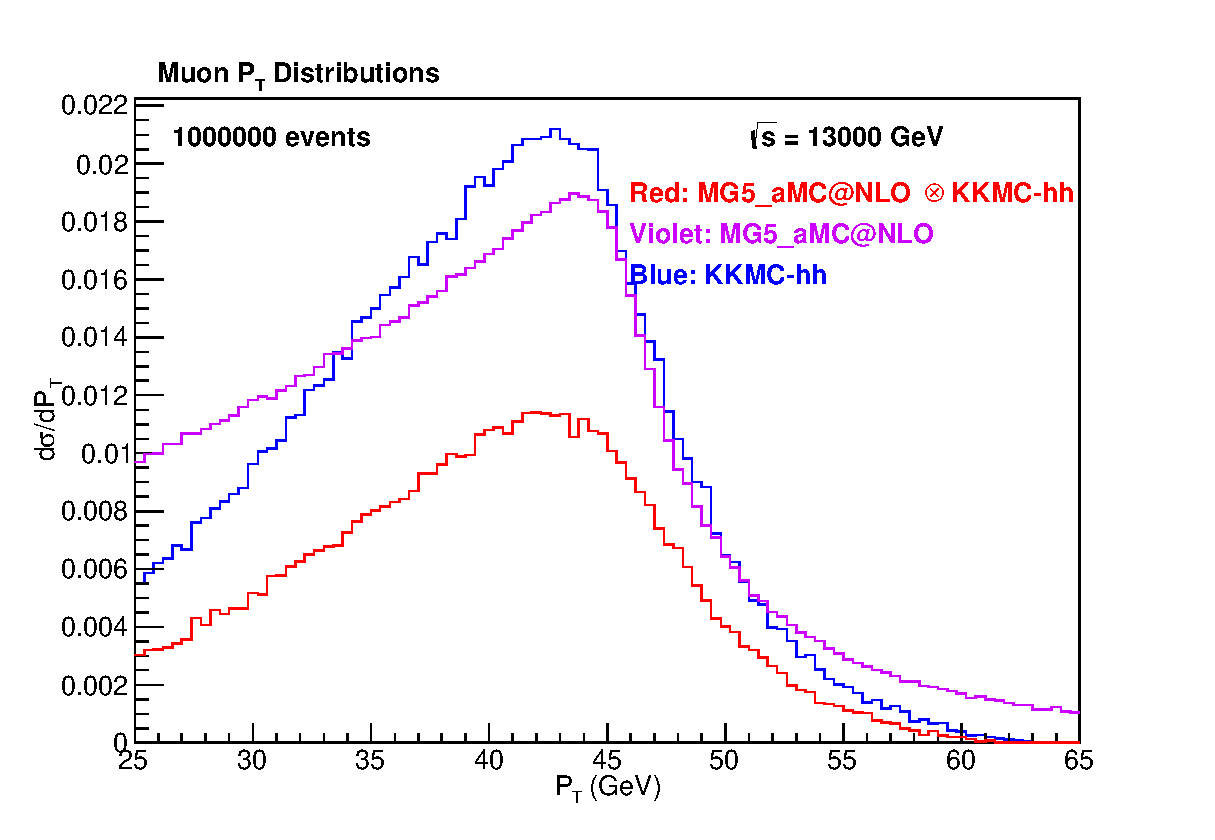
\includegraphics[scale=0.65]{PTL.eps}
		\caption{ Muon transverse momentum distributions for KKMC-hh (blue), MG5\textunderscore aMC@NLO (violet) and MG5\textunderscore aMC@NLO interfaced with KKMC-hh (red) with the cuts specified in the text. }
	\end{center}
\end{figure}

The next quantity we compared is the muon pseudorapidity distribution. The pseudorapidity $\eta$ is a spatial coordinate describing the angle of a particle relative to the beam axis, commonly used in the experimental particle physics. It is defined as 
\begin{equation}
\eta=\log\left(\tan\frac{\theta}{2}\right),
\end{equation} 
where the angle $\theta$ is angle between the particle three-momentum $\vec{p}$ and the positive direction of the beam axis. The pseudorapidity can also be expressed in terms of three-momentum:
\begin{equation}
\eta\equiv\frac{1}{2}\log\left(\frac{|p|+p_L}{|p|-p_L}\right),
\end{equation}
where $p_L$ is the component of the momentum along the beam axis, namely, the longitudinal momentum. From Figure 8.2, we find that interfacing MG5\textunderscore aMC@\newline
NLO with KKMC-hh results an apparent enhancement on the muon pseudorapidity distribution compared with that derived from MG5\textunderscore aMC@NLO.
\begin{figure}
	\begin{center}
		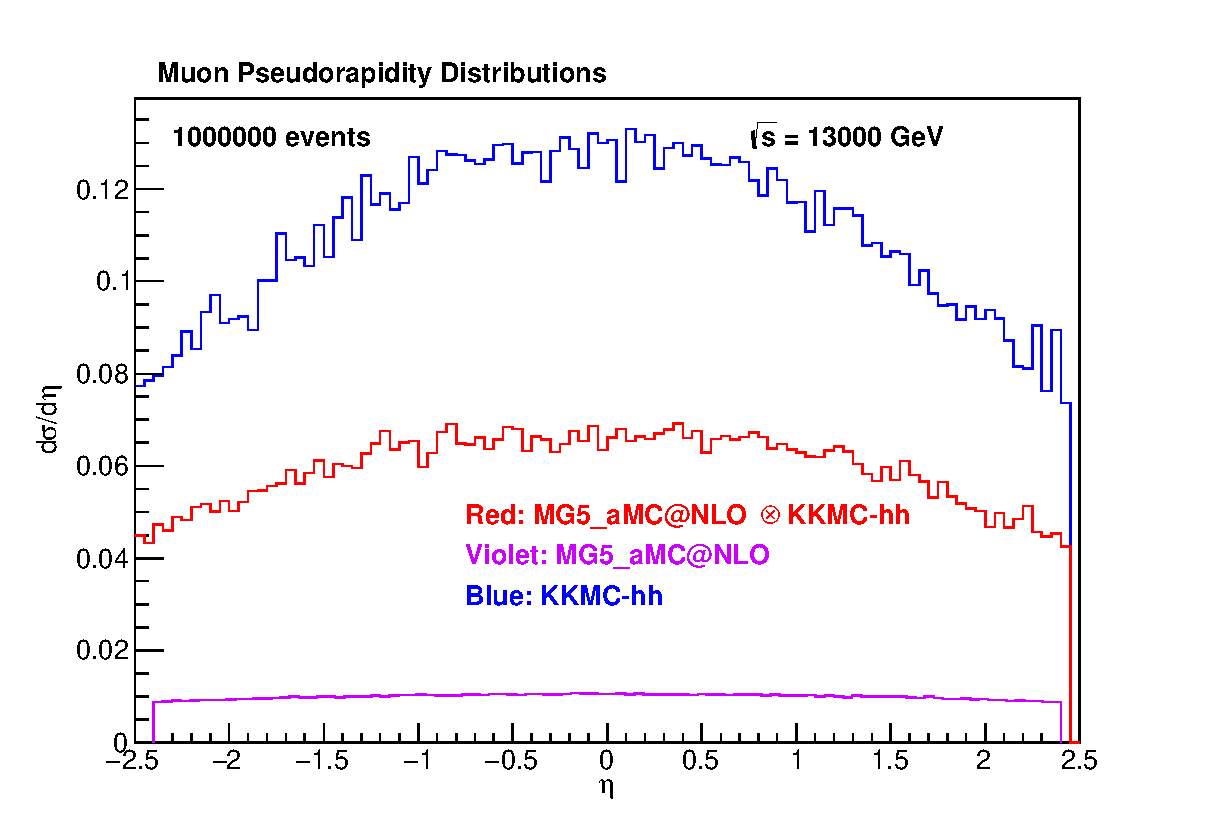
\includegraphics[scale=0.65]{ETA.eps}
		\caption{ Muon pseudorapidity distributions for KKMC-hh (blue), MG5\textunderscore aMC@NLO (violet) and MG5\textunderscore aMC@NLO interfaced with KKMC-hh (red) with the cuts specified in the text. }
	\end{center}
	\end{figure}

We compared not only quantities of the single lepton but those of lepton pairs as well. The dimuon transverse momentum distributions obtained by these three approaches are given in the Figure 8.3. As we can see, the differential cross section calculated by MG5\textunderscore aMC@NLO interfaced with KKMC-hh is larger than that obtained by MG5\textunderscore aMC@NLO only, and the enhancement is from the EW corrections calculated by KKMC-hh. 

And the Figure 8.4 described the dimuon invariant mass distributions. By comparing the dimuon invariant mass distribution derived from MG5\textunderscore aMC@NLO interfaced with KKMC-hh with that from MG5\textunderscore aMC@NLO only, we find there is also an enhancement that is due to the EW corrections provided by KKMC-hh. Besides, we see the resonance peaks near $91\text{ GeV}$ derived from these three generators.
\begin{figure}
	\begin{center}
		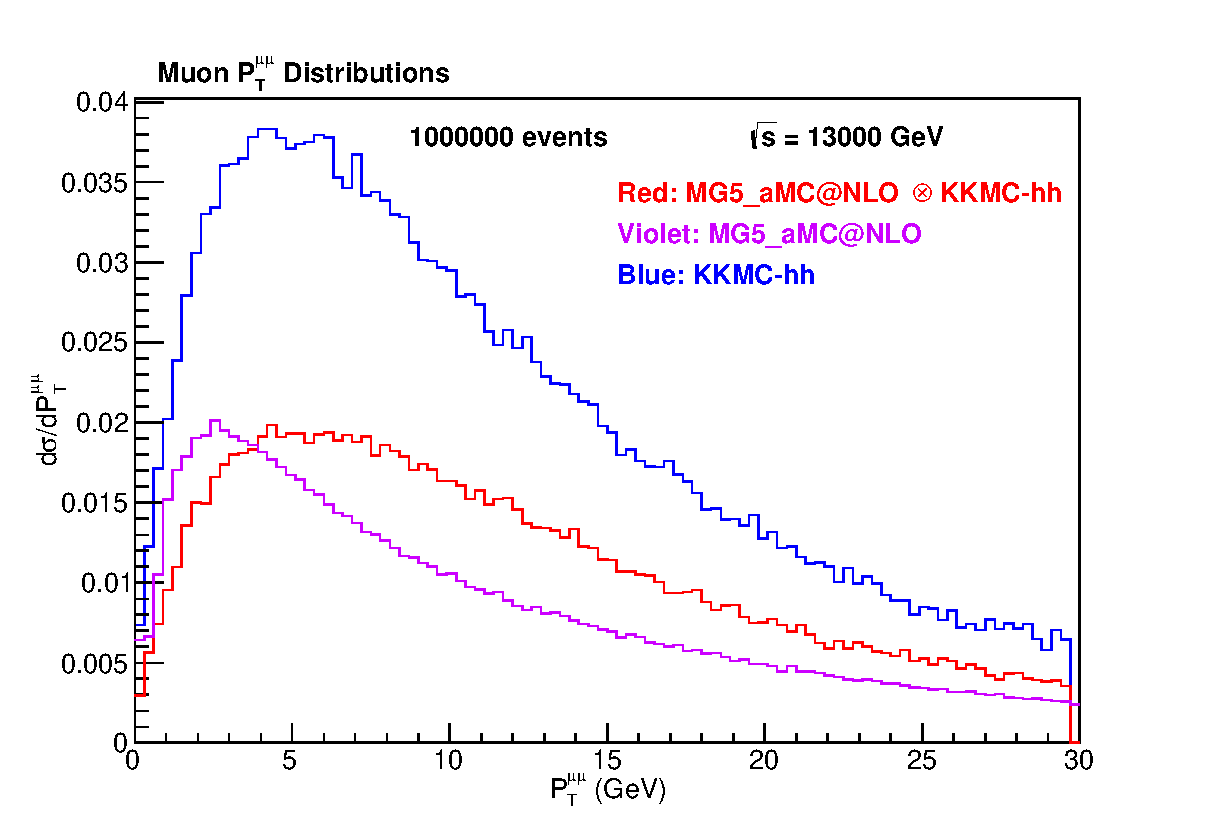
\includegraphics[scale=0.65]{PTLL.eps}
		\caption{ Dimuon transverse momentum distributions for KKMC-hh (blue), MG5\textunderscore aMC@NLO (violet) and MG5\textunderscore aMC@NLO interfaced with KKMC-hh (red) with the cuts specified in the text.  }
	\end{center}
\end{figure}

Finally, let us see the dimuon rapidity distributions in the Figure 8.5. The rapidity is defined as 
\begin{equation}
y\equiv\frac{1}{2}\log\left(\frac{E+p_L}{E-p_L}\right).
\end{equation}
We see that MG5\textunderscore aMC@NLO interfaced with KKMC-hh amplified the dimuon rapidity distribution obtained by MG5\textunderscore aMC@NLO only. The amplification can be viewed as a consequence of the EW corrections.


\begin{figure}
	\begin{center}
		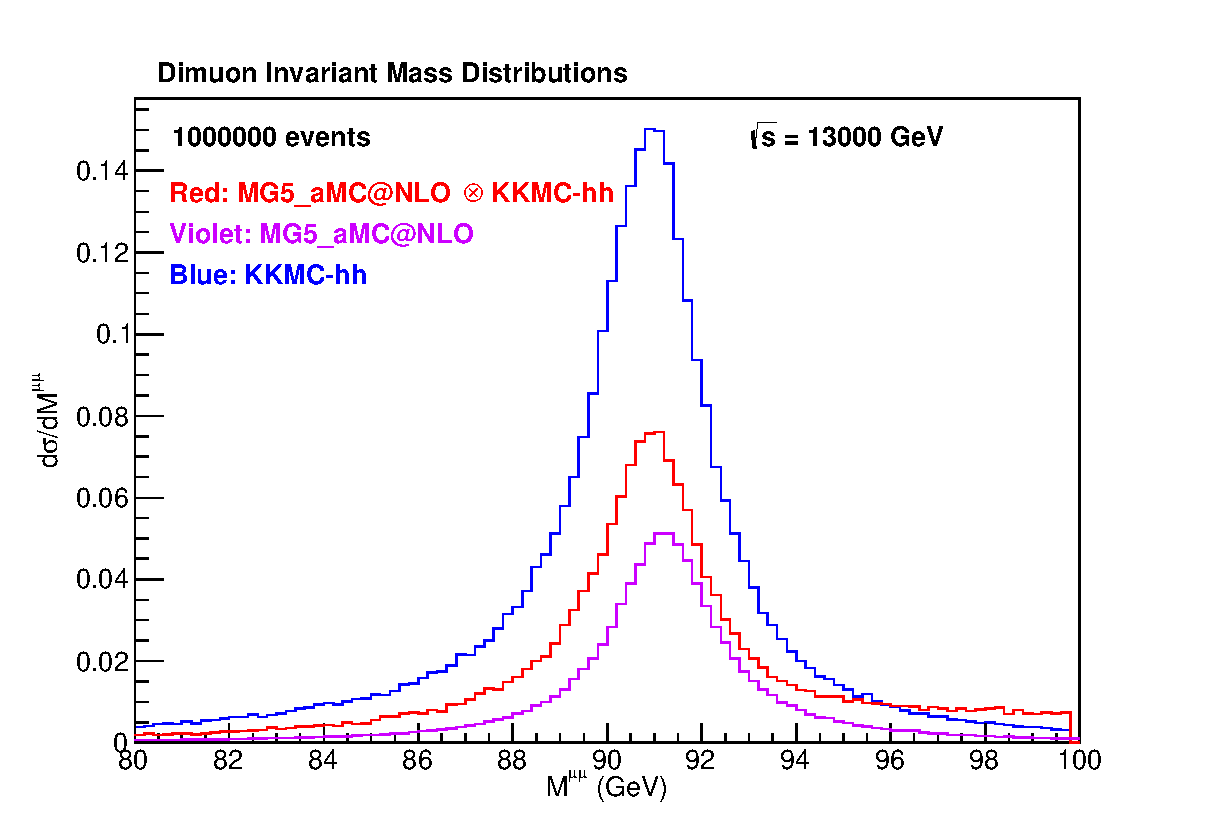
\includegraphics[scale=0.65]{MLL.eps}
		\caption{ Dimuon invariant mass distributions for KKMC-hh (blue), MG5\textunderscore aMC@NLO (violet) and MG5\textunderscore aMC@NLO interfaced with KKMC-hh (red) with the cuts specified in the text. }
	\end{center}
\end{figure} 

In sum, we exhibited the comparisons of the results obtained by MG5\textunderscore aMC@\newline NLO$\otimes$KKMC-hh, MG5\textunderscore aMC@NLO and KKMC-hh. We find that MG5\textunderscore aMC@NLO interfaced with KKMC-hh would enhance the results obtained by MG5\textunderscore aMC@NLO only and the enhancement is due to the EW corrections derived from KKMC-hh.

\begin{figure}
	\begin{center}
		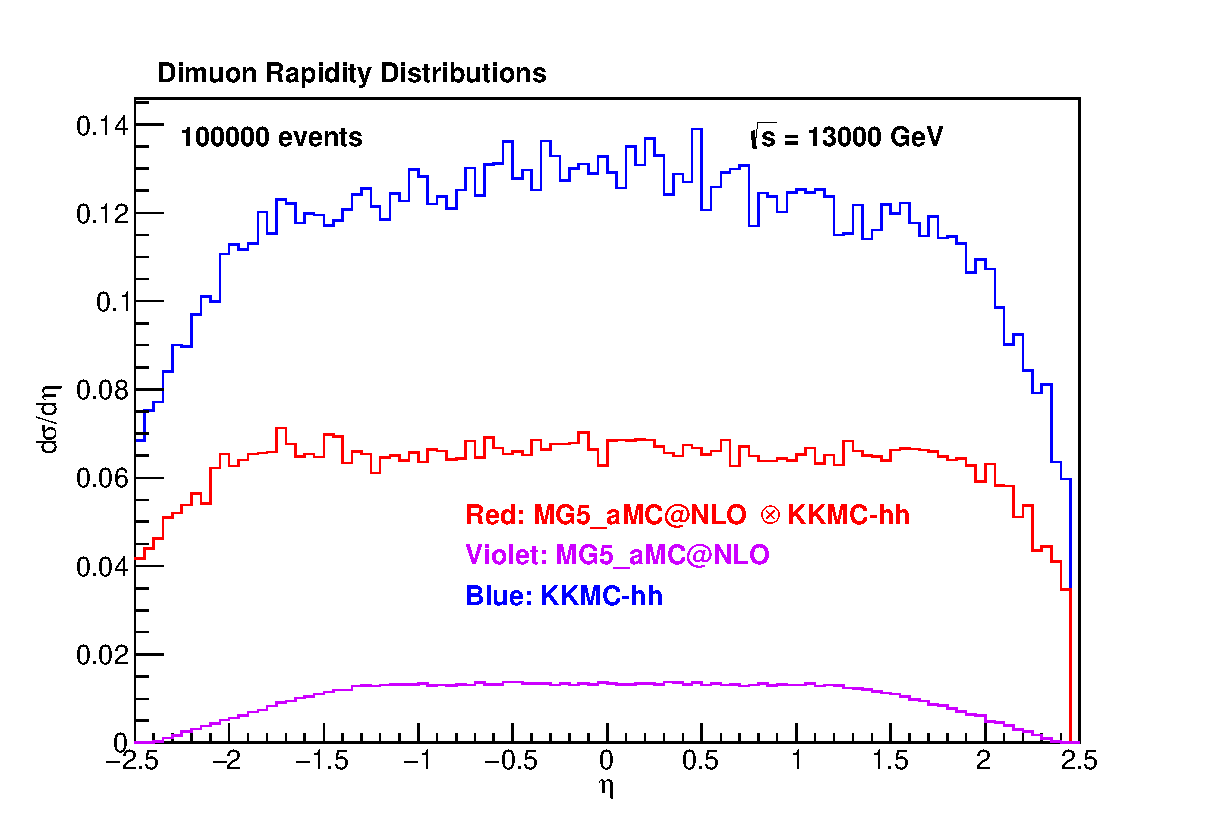
\includegraphics[scale=0.65]{Y.eps}
		\caption{ Dimuon radipity distributions for KKMC-hh (blue), MG5\textunderscore aMC@NLO (violet) and MG5\textunderscore aMC@NLO interfaced with KKMC-hh (red) with the cuts specified in the text. }
	\end{center}
\end{figure}
\chapter{Overall Summary}
In this dissertation, we have developed a new numerical method to calculate the general five-point function, which is important for evaluating one-loop radiative corrections. Our method is developed from the magic spinor product approach in loop integrals proposed by B. F. L. Ward originally, which applied the "Chinese magic" spinor technique to simplify the loop integral so that the $E_0$ could be expressed in terms of $n$-point one-loop integrals $(n\leq4)$. And the $n$-point one-loop integrals $(n\leq4)$ can be calculated numerically by the package LoopTools. Theoretically, the magic spinor product method should provide more efficiency and numerical stability for the evaluation of the general five point function. By comparing the results obtained by our method with those directly obtained from LoopTools, we find that they agreed with each other overall. Such agreements are encouraging.

Additionally, we also developed an approach to achieve the next-to-leading order and the electroweak (EW) exact $O(\alpha_s\otimes\alpha^2L)$ corrections, interfacing MG5\textunderscore aMC@NLO with KKMC-hh by merging their LHE files. We first coded a program to read the event information from the LHE file of MG5\textunderscore aMC@NLO, and then extracted the next-to-leading QCD $O(\alpha_s)$ correction. Combining the NLO QCD corrections computed by MG5\textunderscore aMC@NLO with the basic weight for generating events in the KKMC-hh, we obtained a new basic weight including both the NLO QCD $O(\alpha_s)$ corrections and the EW $O(\alpha^2L)$ corrections. With the help of new basic weight, the new events with $O(\alpha_s\otimes\alpha^2L)$ were generated. We compared the muon transverse momentum distributions, muon pseudorapidity distributions, dimuon invariant mass distributions, dimuon rapidity distributions obtained by KKMC-hh, MG5\textunderscore aMC@NLO and KKMC-hh interfaced with MG5\textunderscore aMC@NLO , at $\sqrt{s}=13\text{ TeV}$ with the ATLAS cuts on the $Z/\gamma^\ast$ production and decay to lepton pairs, respectively. By comparing the results of the Drell-Yan process obtained by these three generators, we find that the results derived from KKMC-hh interfaced with MG5\textunderscore aMC@NLO bring enhancements from those derived from MG5\textunderscore aMC@NLO, which are due to the EW corrections provided by KKMC-hh. We conclude that interfacing MG5\textunderscore aMC@NLO with KKMC-hh would provide a way to achieve the exact $O(\alpha_s\otimes\alpha^2L)$ corrections. 
 

% Appendices (optional)
\multipleappendices % Change to \multipleappendices if you have more than one!
\begin{appendices}
	\chapter{Feynman Rules of the Electroweak SM} 

In this appendix we outline the Feynman rules of electroweak SM in the 't Hooft-Feynman gauge including the counterterms. In the verticles all momenta are set up as incoming. 

	
Propagators:

for gauge bosons $V=\gamma, Z, W$ in the 't Hooft-Feynamn gauge($\xi_i=1$)	

\begin{axopicture}(260,60) %vector boson
	\Photon(20,30)(110,30){3}{6.5}
	\Vertex(20,30){1}
	\Vertex(110,30){1}
	\Text(10,30){$V_\mu$}\Text(120,30){$V_\nu$}\Text(60,40){$k$}
	\Text(170,30){$=\frac{-ig_{\mu\nu}}{k^2-M_V^2}$,}	
\end{axopicture}

for Faddeev-Popov ghosts $G=u^\gamma,u^Z,u^W$

\begin{axopicture}(260,60) %ghost
	\DashLine[arrow](20,30)(110,30){2}
	\Vertex(20,30){1}
	\Vertex(110,30){1}
	\Text(10,30){$G$}\Text(120,30){$\bar{G}$}\Text(60,40){$k$}
	\Text(170,30){$=\frac{i}{k^2-M_G^2}$,}	
\end{axopicture}

for scalar fields $S=H,\chi,\phi$

\begin{axopicture}(260,60) %scalar
	\DashLine[arrow](20,30)(110,30){10}
	\Vertex(20,30){1}
	\Vertex(110,30){1}
	\Text(10,30){$S$}\Text(120,30){${S}$}\Text(60,40){$k$}
	\Text(170,30){$=\frac{i}{k^2-M_S^2}$,}	
\end{axopicture}

and for fermion fields $F=f_i$

\begin{axopicture}(260,60)
	\Line[arrow](20,30)(110,30)
	\Vertex(20,30){1}
	\Vertex(110,30){1}
	\Text(10,30){$F$}\Text(120,30){$\bar{F}$}\Text(60,40){$p$}
	\Text(170,30){$=\frac{i}{\slashed{p}-m_f}$.}	
\end{axopicture}

In the 't Hooft-Feynman gauge we have the following relations:
\begin{equation}
M_{u^\gamma}=0, \quad M_{u^Z}=M_\chi=M_Z, \quad M_{u^\pm}=M_\phi=M_W.
\end{equation}

Tadpole:

\begin{axopicture}(260,60)
	\Line(20,30)(110,30)
	\GCirc(20,30){5.66}{1}	
	\Line(24,26)(16,34)
	\Line(16,26)(24,34)
	\Text(90,40){$S$}
	\Text(170,30){$=i\delta t$.}
\end{axopicture}

$VV$-counterterm:

\begin{axopicture}(260,60) %vector boson
	\Photon(20,30)(110,30){3}{6.5}
	\Vertex(20,30){1}
	\Vertex(110,30){1}
	\Text(10,30){$V_\mu$}\Text(120,30){$V_\nu$}\Text(60,40){$k$}
	\Text(170,30){$=-ig_{\mu\nu}[C_1 k^2-C_2]$}
	\GCirc(65,30){5.66}{1}	
	\Line(61,26)(69,34)
	\Line(69,26)(61,34)	 %counterterm
	
\end{axopicture}
\newline with the actual values of $V_1$, $V_2$ and $C_1$, $C_2$
\begin{eqnarray}
W^+W^-:&& C_1=\delta Z_W, \quad C_2=M_W^2\delta Z_W+\delta M_W^2\nonumber\\
ZZ:&&  C_1=\delta Z_{ZZ}, \quad C_2=M_Z^2\delta Z_{ZZ}+\delta M_Z^2\nonumber\\
AZ:&&  C_1=\frac{1}{2}\delta Z_{AZ}+\frac{1}{2}\delta Z_{ZA}, \quad C_2=M_Z^2\frac{1}{2}\delta Z_{ZA}\nonumber\\
AA:&& C_1=\delta Z_{AA}, \quad C_2=0.
\end{eqnarray}

$SS$-counterterm:

\begin{axopicture}(260,60) %scalar
	\DashLine(20,30)(110,30){10}
	\Vertex(20,30){1}
	\Vertex(110,30){1}
	\Text(10,30){$S_1$}\Text(120,30){${S_2}$}\Text(60,40){$k$}
	\Text(170,30){$=i[C_1 k^2-C_2]$,}
	\GCirc(65,30){5.66}{1}		
	\Line(61,26)(69,34)
	\Line(69,26)(61,34)	 %counterterm
	
\end{axopicture}
\newline with the actual values of $S_1$, $S_2$ and $C_1$, $C_2$
\begin{eqnarray}
HH:C_1=\delta Z_H,\quad C_2=M_H^2\delta Z_H+\delta M_H^2.
\end{eqnarray}

$FF$-counterterm:

\begin{axopicture}(260,60) %fermion
	\Line(20,30)(110,30)
	\Vertex(20,30){1}
	\Vertex(110,30){1}
	\Text(10,30){$F_1$}\Text(120,30){$\bar{F_2}$}\Text(50,40){$p$}
	\Text(170,10){$=i[C_L\slashed{p}\frac{1}{2}(1-\gamma_5)+C_R\slashed{p}\frac{1}{2}(1+\gamma_5)]-C_S^-\slashed{p}\frac{1}{2}(1-\gamma_5-C_S^+\slashed{p}\frac{1}{2}(1+\gamma_5)]$,}
	\GCirc(65,30){5.66}{1}	
	\Line(61,26)(69,34)
	\Line(69,26)(61,34)	 %counterterm
	
\end{axopicture}
\newline with the actual values of $F_1$, $\bar{F}_2$ and $C_L, C_R, C_S^-, C_S^+$
\begin{equation}
f_i\bar{f}_i:\begin{cases} 
C_L=\frac{1}{2}(\delta Z^{f,L}_{ij}+\delta Z^{f,L,\dagger}_{ij}),
\\ C_R=\frac{1}{2}(\delta Z^{f,R}_{ij}+\delta Z^{f,R,\dagger}_{ij})
\\
C^-_S=m_{f,i}\frac{1}{2}\delta Z^{f,L}_{ij}+m_{f,i}\frac{1}{2}\delta Z^{f,R,\dagger}_{ij}+\delta_{ij}\delta m_{f,i},\\
C^+_S=m_{f,i}\frac{1}{2}\delta Z^{f,R}_{ij}+m_{f,i}\frac{1}{2}\delta Z^{f,L,\dagger}_{ij}+\delta_{ij}\delta m_{f,i}.
\end{cases}
\end{equation}


$VVVV$-couping:

\begin{axopicture}(260,130) %fermion
	\Photon(20,110)(65,65){3}{5.5}
	\Photon(65,65)(110,20){3}{5.5}
	\Photon(20,20)(65,65){3}{5.5}
	\Photon(65,65)(110,110){3}{5.5}
	\Vertex(65,65){1}		
	\Text(10,110){$V_{1,\mu}$}
	\Text(10,10){$V_{2,\nu}$}
	\Text(120,10){$V_{4,\sigma}$}
	\Text(120,110){$V_{3,\rho}$}
	\Text(210, 65){$=ie^2C[2g_{\mu\nu}g_{\sigma\rho}-g_{\nu\rho}g_{\mu\sigma}-g_{\rho\mu}g_{\nu\sigma}]$}
	\Vertex(65,65){3}
\end{axopicture}
\newline with the actual values of $V_1$,$V_2$,$V_3$,$V_4$ and $C$
\begin{eqnarray}
W^+W^+W^-W^-:&& C=\frac{1}{s_W^2}\left[1+2\delta Z_e-2\frac{\delta s_W}{s_W}+2\delta Z_W\right]\nonumber\\
W^+W^-ZZ:&& C=-\frac{c_W^2}{s_W^2}\left[1+2\delta Z_e-2\frac{1}{c^2}\frac{\delta s_W}{s_W}+2\delta Z_W+\frac{1}{2}\delta Z_ZZ\right]+\frac{1}{2}\frac{c_W}{s_W}\nonumber\\
W^+W^-AZ:&&C=
\frac{c_W}{s_W}\left[1+2\delta Z_e-\frac{1}{c^2}\frac{\delta s_W}{s_W}+\delta Z_W+\frac{1}{2}\delta Z_{ZZ}+\frac{1}{2}\delta Z_{AA}\right]\nonumber\\
&&-\frac{1}{2}\delta Z_{AZ}
-\frac{1}{2}\frac{c^2_W}{s^2_W}\delta Z_{ZA}\nonumber\\
W^+W^-AA:&&C=-\left[1+2\delta Z_e+\delta Z_W+\delta Z_{AA}\right]+\frac{1}{2}\frac{c_W}{s_W}\delta Z_{ZA}.
\end{eqnarray}

$VVV$-couping:

\begin{axopicture}(260,130) %fermion
	\Photon(10,65)(65,65){3}{5.5} 
	\Photon(65,65)(120,35){3}{5.5}
	\Photon(65,65)(120,105){3}{5.5}
	\Vertex(65,65){1}		
	\Text(10,75){$V_{1,\mu}, k_1$}
	\Text(110,20){$V_{3,\rho},k_3$}
	\Text(110,110){$V_{2,\nu},k_2$}
	\Text(220, 65){$=-ieC[g_{\mu\nu}(k_2-k_1)_\rho-g_{\nu\rho}(k_3-k_2)_\mu$}
	\Text(175,50){$-g_{\rho\mu}(k_1-k_3)_\nu$}
	\Vertex(65,65){3}
\end{axopicture}
\newline with the actual values of $V_1$,$V_2$,$V_3$ and $C$
\begin{eqnarray}
AW^+W^-:&&C=1+\delta Z_e+\delta Z_W+\frac{1}{2}\delta Z_{AA}-\frac{1}{2}\frac{c_W}{s_W}\delta Z_{ZA},\nonumber\\
ZW^+W^-:&&C=-\frac{c_W}{s_W}\left[1+\delta Z_e-\frac{1}{c^2}\frac{\delta s_W}{s_W}+\delta Z_W+\frac{1}{2}\delta Z_{ZZ}\right]+\frac{1}{2}\delta Z_{AZ}.\nonumber\\
\end{eqnarray}

$SSSS$-couping:

\begin{axopicture}(260,130) %fermion
	\Line[dash](20,110)(65,65)
	\Line[dash](65,65)(110,20)
	\Line[dash](20,20)(65,65)
	\Line[dash](65,65)(110,110)
	\Vertex(65,65){1}		
	\Text(10,110){$S_{1}$}
	\Text(10,10){$S_{2}$}
	\Text(120,10){$S_{4,}$}
	\Text(120,110){$S_{3}$}
	\Text(160, 65){$=ie^2C$}
	\Vertex(65,65){3}
\end{axopicture}
\newline with the actual values of $S_1$,$S_2$,$S_3$,$S_4$ and $C$
\begin{eqnarray}
HHHH:&& C=-\frac{3}{4s_W^2}\frac{M^2_H}{M^2_W}\left[1+2\delta Z_e-2\frac{\delta s_W}{s_W}+\frac{\delta M^2_H}{M^2_H}-\frac{\delta M^2_H}{M^2_H}+2\delta Z_H\right],\nonumber\\
HH\chi\chi:&& C=-\frac{1}{4s_W^2}\frac{M^2_H}{M^2_W}\left[1+2\delta Z_e-2\frac{\delta s_W}{s_W}+\frac{\delta M^2_H}{M^2_H}-\frac{\delta M^2_H}{M^2_H}+\delta Z_H\right],\nonumber\\
HH\phi\phi:&& C=-\frac{1}{4s_W^2}\frac{M^2_H}{M^2_W}\left[1+2\delta Z_e-2\frac{\delta s_W}{s_W}+\frac{\delta M^2_H}{M^2_H}-\frac{\delta M^2_H}{M^2_H}+\delta Z_H\right],\nonumber\\
\chi\chi\chi\chi:&& C=-\frac{3}{4s_W^2}\frac{M^2_H}{M^2_W}\left[1+2\delta Z_e-2\frac{\delta s_W}{s_W}+\frac{\delta M^2_H}{M^2_H}-\frac{\delta M^2_H}{M^2_H}\right],\nonumber\\
\chi\chi\phi\phi:&& C=-\frac{1}{4s_W^2}\frac{M^2_H}{M^2_W}\left[1+2\delta Z_e-2\frac{\delta s_W}{s_W}+\frac{\delta M^2_H}{M^2_H}-\frac{\delta M^2_H}{M^2_H}\right],\nonumber\\
\phi\phi\phi\phi:&& C=-\frac{1}{2s_W^2}\frac{M^2_H}{M^2_W}\left[1+2\delta Z_e-2\frac{\delta s_W}{s_W}+\frac{\delta M^2_H}{M^2_H}-\frac{\delta M^2_H}{M^2_H}\right].\nonumber\\
\end{eqnarray}

$SSS$-couping:

\begin{axopicture}(260,130) %fermion
	\Line[dash](10,65)(65,65)
	\Line[dash](65,65)(120,35)
	\Line[dash](65,65)(120,105)
	\Vertex(65,65){1}		
	\Text(10,75){$S_1$}
	\Text(110,25){$S_3$}
	\Text(110,110){$S_2$}
	\Text(160, 65){$=ieC$}
	\Vertex(65,65){3}
\end{axopicture}
\newline with the actual values of $S_1$,$S_2$,$S_3$ and $C$
\begin{eqnarray}
HHH:&&C=-\frac{3}{2s}\frac{M^2_H}{m_W}\left[ 1+\delta Z_e-\frac{\delta s_W}{s_W}+\frac{\delta M^2_H}{M^2_H}-\frac{1}{2}\frac{\delta M^2_W}{M^2_W}+\frac{3}{2}\delta Z_H \right],\nonumber\\
H\chi\chi:&&C=-\frac{1}{2s}\frac{M^2_H}{m_W}\left[ 1+\delta Z_e-\frac{\delta s_W}{s_W}+\frac{\delta M^2_H}{M^2_H}-\frac{1}{2}\frac{\delta M^2_W}{M^2_W}+\frac{1}{2}\delta Z_H \right],\nonumber\\
H\chi\chi:&&C=-\frac{1}{2s}\frac{M^2_H}{m_W}\left[ 1+\delta Z_e-\frac{\delta s_W}{s_W}+\frac{\delta M^2_H}{M^2_H}-\frac{1}{2}\frac{\delta M^2_W}{M^2_W}+\frac{1}{2}\delta Z_H \right].\nonumber\\
\end{eqnarray}


$VVVV$-couping:

\begin{axopicture}(260,130) %fermion
	\Photon(20,110)(65,65){3}{5.5}
	\Line[dash](65,65)(110,20)
	\Photon(20,20)(65,65){3}{5.5}
	\Line[dash](65,65)(110,110)
	\Vertex(65,65){1}		
	\Text(10,110){$V_{1,\mu}$}
	\Text(10,10){$V_{2,\nu}$}
	\Text(120,10){$S_2$}
	\Text(120,110){$S_1$}
	\Text(170, 65){$=ie^2g_{\mu\nu}C$}
	\Vertex(65,65){3}
\end{axopicture}
\newline with the actual values of $V_1$,$V_2$,$S_1$,$S_2$ and $C$
\begin{eqnarray*}
	W^+W^-HH:&&C=\frac{1}{2s^2}\left[ 1+2\delta Z_e-2\frac{\delta s_W}{s_W}+\delta Z_W+\delta Z_H \right],\nonumber\\
	W^+W^-\chi\chi:&&C=\frac{1}{2s^2}\left[ 1+2\delta Z_e-2\frac{\delta s_W}{s_W}+\delta Z_W \right],\nonumber\\
	W^+W^-\phi\phi:&&C=\frac{1}{2s^2}\left[ 1+2\delta Z_e-2\frac{\delta s_W}{s_W}+\delta Z_W \right],\nonumber\\
	ZZ\phi^+\phi^-:&&C=\frac{s^2_W-c^2_W}{2s_W^2c_W^2}\left[ 1+2\delta Z_e+\frac{2}{(s_W^2-c_W^2)c^2_W}\frac{\delta s_W}{s_W}+\delta Z_{ZZ} \right]\nonumber\\
	&&+\frac{s^2_W-c^2_W}{s_Wc_W}\frac{1}{2}\delta Z_{AZ},\nonumber\\
	ZA\phi^+\phi^-:&&C=\frac{s^2_W-c^2_W}{2s_W^2c_W^2}\biggl[ 1+2\delta Z_e+\frac{1}{(s_W^2-c_W^2)c^2_W}\frac{\delta s_W}{s_W}+\frac{1}{2}\delta Z_{ZZ} \nonumber\\
	&&+\frac{1}{2}Z_{AA}\biggr]+\frac{1}{2}\frac{(s_W^2-c_W^2)^2}{2s^2_Wc^2_W}\delta Z_{ZA}+\delta Z_{AZ},\nonumber\\
	AA\phi^+\phi^-:&& C=2[1+2\delta Z_e+\delta Z_{AA}]+\frac{1}{2}\frac{s^2_W-c^2_W}{s_Wc_W}\delta Z_{ZA},\nonumber\\
	ZZHH:&&C=\frac{1}{2s^2_Wc^2_W}\biggl[ 1+2\delta Z_e+2\frac{s^2_W-c^2_W}{c^2_W}\frac{\delta s_W}{s_W}+\delta ZZ+\delta Z_H \biggr],\nonumber\\
	ZZ\chi\chi:&&=\frac{1}{2s^2_Wc^2_W}\biggl[ 1+2\delta Z_e+2\frac{s^2_W-c^2_W}{c^2_W}\frac{\delta s_W}{s_W}+\delta ZZ \biggr],\nonumber\\
	ZAHH:&& C=\frac{1}{2s^2_Wc^2_W}\frac{1}{2}\delta Z_{ZA},\nonumber\\
	ZA\chi\chi:&& C=\frac{1}{2s^2_Wc^2_W}\frac{1}{2}\delta Z_{ZA},\nonumber\\
\end{eqnarray*}
\begin{eqnarray}
W^\pm Z\phi^\mp H:&& C=-\frac{1}{2c_w}\biggl[ 1+\delta Z_e-\frac{\delta c_W}{c_W}+\frac{1}{2}\delta Z_W+\frac{1}{2}\delta Z_H+\frac{1}{2}\delta Z_{ZZ}\biggr]\nonumber\\
&&-\frac{1}{2}\frac{1}{s_W}\delta Z_{AZ} ,\nonumber\\
W^\pm A\phi^\mp H:&& C=-\frac{1}{2s_w}\biggl[ 1+\delta Z_e-\frac{\delta s_W}{s_W}+\frac{1}{2}\delta Z_W+\frac{1}{2}\delta Z_H+\frac{1}{2}\delta Z_{AA} \biggr]\nonumber\\
&&-\frac{1}{2}\frac{1}{c_W}\delta Z_{ZA},\nonumber\\
W^\pm Z\phi^\mp \chi:&& C=\mp\frac{i}{2c_w}\biggl[ 1+\delta Z_e-\frac{\delta c_W}{c_W}+\frac{1}{2}\delta Z_W+\frac{1}{2}\delta Z_{ZZ} \biggr]\mp\frac{1}{2}\frac{i}{2s_W}\delta Z_{AZ},\nonumber\\
W^\pm Z\phi^\mp \chi:&& C=\mp\frac{i}{2s_w}\biggl[ 1+\delta Z_e-\frac{\delta s_W}{s_W}+\frac{1}{2}\delta Z_W+\frac{1}{2}\delta Z_{AA} \biggr]\mp\frac{1}{2}\frac{i}{2c_W}\delta Z_{ZA}.\nonumber\\
\end{eqnarray}

$VSS$-couping:

\begin{axopicture}(260,130) %fermion
	\Photon(10,65)(65,65){3}{5.5}
	\Line[dash](65,65)(120,35)
	\Line[dash](65,65)(120,105)
	\Vertex(65,65){1}		
	\Text(10,75){$V_\mu$}
	\Text(110,25){$S_2,k_2$}
	\Text(110,110){$S_1,k_1$}
	\Text(180, 65){$=ieC(k_1-k_2)_\mu$}
	\Vertex(65,65){3}
\end{axopicture}
\newline with the actual values of $V$, $S_1$,$S_2$ and $C$
\begin{eqnarray}
A\chi H:&& C=-\frac{1}{2}\frac{i}{2c_Ws_W}\delta Z_{ZA},\nonumber\\
Z\chi H:&& C=-\frac{i}{2c_ws_W}\biggl[ 1+\delta Z_e+\frac{s^2_W-c^2_W}{c^2_W}\frac{\delta s_W}{s_W}+\frac{1}{2}\delta Z_H+\frac{1}{2}\delta Z_{ZZ} \biggr],\nonumber\\
A\phi^+\phi^-:&& C=-\biggl[ 1+\delta Z_e+\frac{1}{2}\delta Z_{AA}+\frac{1}{2}\frac{s^2_W-c^2_W}{2s_Wc_W}\delta Z_{ZA} \biggr],\nonumber\\
Z\phi^+\phi^-:&& C=-\frac{s^2_w-c^2_W}{2s_Wc_W}\biggl[ 1+\delta Z_e+\frac{1}{(s^2_W-c^2_W)c^2_W}\frac{\delta s_w}{s_W}+\frac{1}{2}\delta Z_{ZZ} \biggr]-\frac{1}{2}\delta Z_{AZ},\nonumber\\
W^\pm\phi^\pm H:&& C=\mp\frac{1}{2s_W}\biggl[ 1+\delta Z_e-\frac{\delta s_W}{s_W}+\frac{1}{2}\delta Z_W+\frac{1}{2}\delta Z_H \biggr],\nonumber\\
W^\pm\phi^\pm \chi:&& C=-\frac{i}{2s_W}\biggl[ 1+\delta Z_e-\frac{\delta s_W}{s_W}+\frac{1}{2}\delta Z_W \biggr].\nonumber\\
\end{eqnarray}

$SVV$-couping:

\begin{axopicture}(260,130) %fermion
	\Line[dash](10,65)(65,65)
	\Photon(65,65)(120,35){3}{5.5}
	\Photon(65,65)(120,105){3}{5.5}
	\Vertex(65,65){1}		
	\Text(10,75){$S$}
	\Text(110,25){$V_{2,\rho}$}
	\Text(110,110){$V_{1,\nu}$}
	\Text(170, 65){$=ieg_{\mu\nu}C$}
	\Vertex(65,65){3}
\end{axopicture}
\newline with the actual values of $S$, $V_1$,$V_2$ and $C$
\begin{eqnarray}
HW^+W^-:&& C=M_W\frac{1}{s_W}\biggl[ 1+\delta Z_e-\frac{\delta s_W}{s_W}+\frac{1}{2}\frac{\delta M^2_W}{M_W^2}+\frac{1}{2}\delta Z_H+\delta Z_W \biggr]\nonumber\\
HZZ:&& C=M_W\frac{1}{s_Wc^2_W}\biggl[ 1+\delta Z_e+\frac{2s^2_W-c^2_W}{c^2_W}\frac{\delta s_W}{s_W}+\frac{1}{2}\frac{\delta M^2_W}{M_W^2}+\frac{1}{2}\delta Z_H+\delta Z_{ZZ} \biggr],\nonumber\\
HZA:&& C=M_W\frac{1}{s_Wc^2_W}\frac{1}{2}\delta Z_{ZA},\nonumber\\
\phi^\pm
W^\mp Z:&& C=-M_W\frac{s_W}{c_W}\biggl[ 1+\delta Z_e+\frac{1}{c^2_W}\frac{\delta s_W}{s_W}+\frac{1}{2}\frac{\delta M^2_W}{M_W^2}+\frac{1}{2}\delta Z_W+\frac{1}{2}\delta Z_{ZZ} \biggr],\nonumber\\
\phi^\pm W^\mp A:&& C=-M_W\biggl[ 1+\delta Z_e+\frac{1}{2}\frac{\delta M^2_W}{M_W^2}+\frac{1}{2}\delta Z_W+\frac{1}{2}\delta Z_{AA} \biggr]-M_W\frac{s_W}{c_W}\frac{1}{2}\delta Z_{ZA}.\nonumber\\
\end{eqnarray}

$VFF$-couping:

\begin{axopicture}(260,130) %fermion
	\Photon(10,65)(65,65){3}{5.5}
	\Line[arrow](120,35)(65,65)
	\Line[arrow](65,65)(120,105)
	\Vertex(65,65){1}		
	\Text(10,75){$V_\mu$}
	\Text(110,25){$F_2$}
	\Text(110,110){$\bar{F}_1$}
	\Text(180, 65){$=ie\gamma_{\mu}(C^-\omega_-+C^+\omega_+)$}
	\Vertex(65,65){3}
\end{axopicture}
\newline with the actual values of $V$, $\bar{F}_1$,$F_2$ and $C^+$ and $C^-$
\begin{eqnarray}
\gamma\bar{f}_if_j:&&
\begin{cases}
C^+=-Q_f[ \delta_{ij}( 1+\delta Z_e+\frac{1}{2}\delta Z_{AA})+\frac{1}{2}(\delta Z^{f,R}_{ij}+\delta Z^{f,R\dagger}_{ij})]+\delta_{ij}g^+_f\frac{1}{2}\delta Z_{ZA},\\
C^-=-Q_f[ \delta_{ij}( 1+\delta Z_e+\frac{1}{2}\delta Z_{AA})+\frac{1}{2}(\delta Z^{f,L}_{ij}+\delta Z^{f,L\dagger}_{ij})]+\delta_{ij}g^-_f\frac{1}{2}\delta Z_{ZA},\\
\end{cases}\nonumber\\
Z\bar{f}_if_j:&&
\begin{cases}
C^+=g^+_f[ \delta_{ij}( 1+\frac{\delta g^+_f}{g^+_f}+\frac{1}{2}\delta Z_{ZZ})+\frac{1}{2}(\delta Z^{f,R}_{ij}+\delta Z^{f,R\dagger}_{ij})]-\delta_{ij}Q_f\frac{1}{2}\delta Z_{AZ},\\
C^-=g^+_f[ \delta_{ij}( 1+\frac{\delta g^-_f}{g^-_f}+\frac{1}{2}\delta Z_{ZZ})+\frac{1}{2}(\delta Z^{f,L}_{ij}+\delta Z^{f,L\dagger}_{ij})]-\delta_{ij}Q_f\frac{1}{2}\delta Z_{AZ},\\
\end{cases}\nonumber\\
W^+\bar{u}_id_j:&&
\begin{cases}
C^+=0,\\
C^-=\frac{1}{\sqrt{2}s_W}\biggl[V_{ij}\biggl(1+\delta Z_e-\frac{\delta S_W}{s_W}+\frac{1}{2}\delta Z_W\biggr)+\delta V_{ij}
+\frac{1}{2}\sum_k(\delta Z^{u,L\dagger}_{jk}V_{kj}\\
\quad\quad+V_{ik}\delta Z^{d,L}_{kj})\biggr],
\end{cases}\nonumber\\
W^-\bar{d}_ju_i:&&
\begin{cases}
C^+=0,\\
C^-=\frac{1}{\sqrt{2}s_W}\biggl[V_{ji}^\dagger\biggl(1+\delta Z_e-\frac{\delta S_W}{s_W}+\frac{1}{2}\delta Z_W\biggr)+\delta V_{ji}^\dagger
+\frac{1}{2}\sum_k(\delta Z^{d,L\dagger}_{jk}V_{ki}^\dagger\\
\quad\quad+V_{jk}^\dagger\delta Z^{u,L}_{ki})\biggr],
\end{cases}\nonumber\\
W^+\bar{\nu}_il_j:&&
\begin{cases}
C^+=0,\\
C^-=\frac{1}{\sqrt{2}s_W}\delta_{ij}\biggl[ 1+\delta Z_e-\frac{\delta s_W}{s_W}+\frac{1}{2}\delta Z_W+\frac{1}{2}(\delta Z^{\nu,L\dagger})_{ii}+\delta Z^{l,L}_{ii} \biggr],
\end{cases}\nonumber\\
W^-\bar{l}_j\nu_i:&&
\begin{cases}
C^+=0,\\
C^-=\frac{1}{\sqrt{2}s_W}\delta_{ij}\biggl[ 1+\delta Z_e-\frac{\delta s_W}{s_W}+\frac{1}{2}\delta Z_W+\frac{1}{2}(\delta Z^{l,L\dagger})_{ii}+\delta Z^{\nu,L}_{ii} \biggr],
\end{cases}
\end{eqnarray}
where
\begin{eqnarray}
&g^+_f=-\frac{s_W0}{c_W}Q_f,&\delta g^+_f=-\frac{s_W}{c_W}Q_f\biggl[ \delta Z_e+\frac{1}{c_W^2}\frac{\delta s_W}{s_W} \biggr],\nonumber\\
&g^-_f=\frac{I^3_{W,f}-s^2_WQ_f}{s_Wc_W},&\delta g^+_f=\frac{I^2_{W,f}}{s_Wc_W}Q_f\biggl[ \delta Z_e+\frac{s^2_W-c^2_W}{c_W^2}\frac{\delta s_W}{s_W} \biggr]+\delta g^+_f.
\end{eqnarray}
The vector and axial vector couplings fo the $Z$-boson are given by
\begin{equation}
v_f=\frac{1}{2}(g^-+g^+)=\frac{I^3_{W,f}-2s_W^2Q_f}{2s_Wc_W},\quad a_f=\frac{1}{2}(g^-_f-g^+_f)=\frac{I^3_{W,f}}{2s_Wc_W}.
\end{equation}
\newpage
$SFF$-couping:

\begin{axopicture}(260,130) %fermion
	\Line[dash](10,65)(65,65)
	\Line[arrow](120,35)(65,65)
	\Line[arrow](65,65)(120,105)
	\Vertex(65,65){1}		
	\Text(10,75){$V_\mu$}
	\Text(110,25){$F_2$}
	\Text(110,110){$\bar{F}_1$}
	\Text(180, 65){$=ie(C^-\omega_-+C^+\omega_+)$}
	\Vertex(65,65){3}
\end{axopicture}
\newline with the actual values of $S$, $\bar{F}_1$,$F_2$ and $C^+$ and $C^-$
\begin{eqnarray*}
	H\bar{f}_if_j:&&\begin{cases}
		C^+=-\frac{1}{2s_W}\frac{m_{f,i}}{M_W}\biggl[ \delta_{ij}\biggl(  1+\delta Z_e-\frac{\delta s_w}{s_W}+\frac{\delta m_{f,i}}{m_{f,i}}-\frac{\delta M_W}{M_W}+\frac{1}{2}\delta Z_H \biggr)\\
		\quad\quad\quad+\frac{1}{2}(\delta Z^{f,R}_{ij}+\delta Z^{f,R\dagger}_{ij}) \biggr],\\
		C^-=-\frac{1}{2s_W}\frac{m_{f,i}}{M_W}\biggl[ \delta_{ij}\biggl(  1+\delta Z_e-\frac{\delta s_w}{s_W}+\frac{\delta m_{f,i}}{m_{f,i}}-\frac{\delta M_W}{M_W}+\frac{1}{2}\delta Z_H \biggr)\\
		\quad\quad\quad+\frac{1}{2}(\delta Z^{f,L}_{ij}+\delta Z^{f,L\dagger}_{ij}) \biggr],
	\end{cases}\nonumber\\
	\chi\bar{f}_if_j:&&\begin{cases}
		C^+=i\frac{1}{2s_W}2I^3_{W,f}\frac{m_{f,i}}{M_W}\biggl[ \delta_{ij}\biggl(  1+\delta Z_e-\frac{\delta s_w}{s_W}+\frac{\delta m_{f,i}}{m_{f,i}}-\frac{\delta M_W}{M_W} \biggr)\\
		\quad\quad\quad+\frac{1}{2}(\delta Z^{f,R}_{ij}+\delta Z^{f,R\dagger}_{ij}) \biggr],\\
		C^-=-i\frac{1}{2s_W}2I^3_{W,f}\frac{m_{f,i}}{M_W}\biggl[ \delta_{ij}\biggl(  1+\delta Z_e-\frac{\delta s_w}{s_W}+\frac{\delta m_{f,i}}{m_{f,i}}-\frac{\delta M_W}{M_W} \biggr)\\
		\quad\quad\quad+\frac{1}{2}(\delta Z^{f,L}_{ij}+\delta Z^{f,L\dagger}_{ij}) \biggr],
	\end{cases}\nonumber\\
	\phi^+\bar{u}_id_j:&&
	\begin{cases}
		C^+=-\frac{1}{\sqrt{2}s_W}\frac{m_{d,j}}{M_W}\biggl[ V_{ij}\biggl( 1+\delta Z_e-\frac{\delta s_W}{s_W}+\frac{\delta m_{d,j}}{m_{d,j}}-\frac{\delta M_W}{M_W}+\delta V_{ij}\\
		\quad\quad\quad +\frac{1}{2}\sum_k(\delta Z^{u,R\dagger}_{ik}V_{kj}+V_{ik}\delta Z^{d,R}_{kj}) \biggr) \biggr],\\
		C^-=\frac{1}{\sqrt{2}s_W}\frac{m_{u,j}}{M_W}\biggl[ V_{ij}\biggl( 1+\delta Z_e-\frac{\delta s_W}{s_W}+\frac{\delta m_{u,j}}{m_{u,j}}-\frac{\delta M_W}{M_W}+\delta V_{ij}\\
		\quad\quad\quad +\frac{1}{2}\sum_k(\delta Z^{u,L\dagger}_{ik}V_{kj}+V_{ik}\delta Z^{d,L}_{kj}) \biggr) \biggr],\\
	\end{cases}\nonumber\\
\end{eqnarray*}
\begin{eqnarray}
\phi^-\bar{d}_ju_i:&&
\begin{cases}
C^+=\frac{1}{\sqrt{2}s_W}\frac{m_{u,i}}{M_W}\biggl[ V^\dagger_{ji}\biggl( 1+\delta Z_e-\frac{\delta s_W}{s_W}+\frac{\delta m_{u,j}}{m_{u,j}}-\frac{\delta M_W}{M_W}+\delta V_{ji}^\dagger\\
\quad\quad\quad +\frac{1}{2}\sum_k(\delta Z^{d,R\dagger}_{jk}V_{ki}^\dagger+V_{jk}^\dagger\delta Z^{u,R}_{ki}) \biggr) \biggr],\\
C^-=-\frac{1}{\sqrt{2}s_W}\frac{m_{d,i}}{M_W}\biggl[ V^\dagger_{ji}\biggl( 1+\delta Z_e-\frac{\delta s_W}{s_W}+\frac{\delta m_{d,j}}{m_{d,j}}-\frac{\delta M_W}{M_W}+\delta V_{ji}^\dagger\\
\quad\quad\quad +\frac{1}{2}\sum_k(\delta Z^{d,L\dagger}_{jk}V_{ki}^\dagger+V_{jk}^\dagger\delta Z^{u,L}_{ki}) \biggr) \biggr],\\
\end{cases}\nonumber\\
\phi^+\bar{\nu}_il_j:&&
\begin{cases}
C^+=-\frac{1}{\sqrt{2}s_W}\frac{m_{i,j}}{M_W}\delta_{ij}\biggl[  1+\delta Z_e-\frac{\delta s_W}{s_W}+\frac{\delta m_{i,j}}{m_{i,j}}-\frac{\delta M_W}{M_W} +\frac{1}{2}\biggl(\delta Z^{\nu,R\dagger}_{ii}+\delta Z^{l,R}_{ii}  \biggr) \biggr],\\
C^-=0,
\end{cases}\nonumber\\
\phi^-\bar{l}_j\nu_i:&&
\begin{cases}
C^+=0,\\
C^-=-\frac{1}{\sqrt{2}s_W}\frac{m_{i,j}}{M_W}\delta_{ij}\biggl[  1+\delta Z_e-\frac{\delta s_W}{s_W}+\frac{\delta m_{i,j}}{m_{i,j}}-\frac{\delta M_W}{M_W} +\frac{1}{2}\biggl(\delta Z^{l,L\dagger}_{ii}+\delta Z^{\nu,L}_{ii}  \biggr) \biggr].
\end{cases}\nonumber\\
\end{eqnarray}

$VGG$-couping:

\begin{axopicture}(260,130) %fermion
	\Photon(10,65)(65,65){3}{5.5}
	\Line[arrow,dash](120,35)(65,65)
	\Line[arrow,dash](65,65)(120,105)
	\Vertex(65,65){1}		
	\Text(10,75){$V_\mu$}
	\Text(110,25){$G_2,k_2$}
	\Text(110,110){$\bar{G}_1,k_1$}
	\Text(180, 65){$=iek_{1,\mu}C$}
	\Vertex(65,65){3}
\end{axopicture}
\newline with the actual values of $V$, $\bar{G}_1$,$G_2$ and $C$
\begin{eqnarray}
A\bar{u}^\pm u^\pm:&& C=\pm\biggl[1+\delta Z_e+\frac{1}{2}\delta Z_{AA}\biggr]\mp\frac{c_W}{s_W}\frac{1}{2}\delta Z_{AA},\nonumber\\
Z\bar{u}^\pm u^\pm:&& C=\mp\biggl[1+\delta Z_e-\frac{1}{c_W^2}\frac{\delta s_W}{s_W}+\frac{1}{2}\delta Z_{ZZ}\biggr]\pm\frac{1}{2}\delta Z_{AZ},\nonumber\\
W^\pm\bar{u}^\pm u^Z:&& C=\pm\biggl[1+\delta Z_e-\frac{1}{c_W^2}\frac{\delta s_W}{s_W}+\frac{1}{2}\delta Z_{W}\biggr],\nonumber\\
W^\pm\bar{u}^Z u^\mp:&& C=\mp\biggl[1+\delta Z_e-\frac{1}{c_W^2}\frac{\delta s_W}{s_W}+\frac{1}{2}\delta Z_{W}\biggr],\nonumber\\
W^\pm\bar{u}^\pm u^\gamma:&& C=\mp\biggl[1+\delta Z_e+\frac{1}{2}\delta Z_{W}\biggr],\nonumber\\
W^\pm\bar{u}^\gamma u^\pm:&& C=\pm\biggl[1+\delta Z_e+\frac{1}{2}\delta Z_{W}\biggr].
\end{eqnarray}

$SGG$-couping:

\begin{axopicture}(260,130) %fermion
	\Photon(10,65)(65,65){3}{5.5}
	\Line[arrow,dash](120,35)(65,65)
	\Line[arrow,dash](65,65)(120,105)
	\Vertex(65,65){1}		
	\Text(10,75){$V_\mu$}
	\Text(110,25){$G_2$}
	\Text(110,110){$\bar{G}_1$}
	\Text(180, 65){$=ieC$}
	\Vertex(65,65){3}
\end{axopicture}
\newline with the actual values of $S$, $\bar{G}_1$,$G_2$ and $C$
\begin{eqnarray}
H\bar{u}^Zu^Z:&&C=-\frac{1}{2s_Wc_W^2}M_W\biggl[ 1+\delta Z_e+\frac{2s_W^2-c_W^2}{c^2_W}\frac{\delta s_W}{s_W}+\frac{1}{2}\frac{\delta M^2_W}{M^2_W}+\frac{1}{2}\delta Z_H \biggr],\nonumber\\
H\bar{u}^\pm u^\pm:&&C=-\frac{1}{2s_W}M_W\biggl[ 1+\delta Z_e-\frac{\delta s_W}{s_W}+\frac{1}{2}\frac{\delta M^2_W}{M^2_W}+\frac{1}{2}\delta Z_H \biggr],\nonumber\\
\chi\bar{u}^\pm u^\pm:&&C=\mp i\frac{1}{2s_W}M_W\biggl[ 1+\delta Z_e-\frac{\delta s_W}{s_W}+\frac{1}{2}\frac{\delta M^2_W}{M^2_W} \biggr],\nonumber\\
\phi^\pm\bar{u}^Zu^\mp:&&C=\frac{1}{2s_Wc_W}M_W\biggl[ 1+\delta Z_e+\frac{s_W^2-c_W^2}{c^2_W}\frac{\delta s_W}{s_W}+\frac{1}{2}\frac{\delta M^2_W}{M^2_W} \biggr],\nonumber\\
\phi^\pm\bar{u}^\pm u^Z:&&C=\frac{s^2_W-c^2_W}{2s_Wc_W}M_W\biggl[ 1+\delta Z_e+\frac{1}{(s_W^2-c_W^2)c^2_W}\frac{\delta s_W}{s_W}+\frac{1}{2}\frac{\delta M^2_W}{M^2_W} \biggr],\nonumber\\
\phi^\pm\bar{u}^\pm u^\gamma:&&C=M_W\biggl[ 1+\delta Z_e+\frac{1}{2}\frac{\delta M^2_W}{M^2_W} \biggr].\nonumber\\
\end{eqnarray}


	\chapter{Feynman Rules of Quantum Chromodynamics}

In this appendix we outline the Feynman rules of quantum chromodynamics including the counterterms.
\begin{eqnarray}
V_{\mu_1\mu_2\mu_3}(k_1,k_2,k_3)&=&(k_1-k_2)_{\mu_3}g_{\mu_1\mu_2}+(k_2-k_3)_{\mu_1}g_{\mu_2\mu_3}+(k_3-k_1)_{\mu_2}g_{\mu_3\mu_1}\nonumber\\
\end{eqnarray}
\begin{eqnarray}
W^{a_1\cdots a_4}_{\mu_1\cdots\mu_4}&=&(f^{13,24}-f^{14,32})g_{\mu_1\mu_2}g_{\mu_3\mu_4}+(f^{12,34}-f^{14,23})g_{\mu_1\mu_3}g_{\mu_2\mu_4}\nonumber\\
&&+(f^{13,42}-f^{12,34})g_{\mu_1\mu_4}g_{\mu_3\mu_2}
\end{eqnarray}
\begin{eqnarray}
f^{ij,kl}&=&f^{a_ia_ja}f^{a_ka_la}
\end{eqnarray}

	
Propagators:
\newline
Gluons $A$

\begin{axopicture}(260,60) %vector boson
	\Gluon(20,30)(110,30){4}{6.5}
	\Vertex(20,30){1}
	\Vertex(110,30){1}
	\Text(10,30){$a\mu$}\Text(120,30){$b\nu$}\Text(60,40){$k$}
	\Text(210,30){$=\delta_{ab}\frac{1}{k^2}\biggl( g_{\mu\nu}-(1-\alpha)\frac{k_\mu k_\nu}{k^2} \biggr)$,}	
\end{axopicture}
\newline
Faddeev-Popov ghosts $\chi$

\begin{axopicture}(260,60) %ghost
	\DashLine[arrow](110,30)(20,30){2}
	\Vertex(20,30){1}
	\Vertex(110,30){1}
	\Text(10,30){$a$}\Text(120,30){$\bar{b}$}\Text(60,40){$k$}
	\Text(170,30){$=\delta_{ab}\frac{-1}{k^2}$,}	
\end{axopicture}
\newline
Quark fields $\psi$

\begin{axopicture}(260,60)
	\Line[arrow](110,30)(20,30)
	\Vertex(20,30){1}
	\Vertex(110,30){1}
	\Text(10,30){$a$}\Text(120,30){$b$}\Text(60,40){$p$}
	\Text(170,30){$=\delta_{ij}\frac{1}{m_f-\slashed{p}}$.}	
\end{axopicture}
\newline
Gluon-counterterm

\begin{axopicture}(260,60) %vector boson
	\Gluon(20,30)(59.34,30){4}{3}
	\Gluon(59.34,30)(110,30){4}{3}
	\Vertex(20,30){1}
	\Vertex(110,30){1}
	\Text(10,30){$a\mu$}\Text(120,30){$b\nu$}\Text(65,47){$k$}
	\Text(210,30){$=(Z_3-1)\delta_{ab}(k_\mu k_\nu-k^2g_{\mu\nu})$}
	\GCirc(65,30){5.66}{1}	
	\Line(61,26)(69,34)
	\Line(69,26)(61,34)	 %counterterm
\end{axopicture}
\newline
Faddeev-Popov ghost counterterm

\begin{axopicture}(260,60) %scalar
	\DashLine[arrow](59.34,30)(20,30){2}
	\DashLine[arrow](110,30)(59.34,30){2}
	\Vertex(20,30){1}
	\Vertex(110,30){1}
	\Text(10,30){$a$}\Text(120,30){$b$}\Text(65,47){$k$}
	\Text(170,30){$=(\widetilde{Z}_3-1)\delta_{ab}k^2$,}
	\GCirc(65,30){5.66}{1}		
	\Line(61,26)(69,34)
	\Line(69,26)(61,34)	 %counterterm
	
\end{axopicture}
\newline
Fermion counterterm

\begin{axopicture}(260,60) %fermion
	\Line[arrow](59.34,30)(20,30)
	\Line[arrow](110,30)(59.34,30)
	\Vertex(20,30){1}
	\Vertex(110,30){1}
	\Text(10,30){$i$}\Text(120,30){$j$}\Text(50,40){$p$}
	\Text(210,30){$=[(Z_2-1)\slashed p-(Z_2Z_m-1)m_R]\delta_{ij}$,}
	\GCirc(65,30){5.66}{1}	
	\Line(61,26)(69,34)
	\Line(69,26)(61,34)	 %counterterm
\end{axopicture}	


Vertices:	
\newline
Three-gluon vertex

\begin{axopicture}(260,130) %fermion
	\Gluon(10,65)(65,65){4}{5.5} 
	\Gluon(65,65)(120,35){4}{5.5}
	\Gluon(65,65)(120,105){4}{5.5}
	\Vertex(65,65){1}		
	\Text(10,75){$a_1, \mu_1$}
	\Text(110,20){$a_3, \mu_3$}
	\Text(110,115){$a_2, \mu_2$}
	\Text(220, 65){$=-igf^{a_1a_2a_3}V_{\mu_1\mu_2\mu_3}(k_1,k_2,k_3)$}
	\Vertex(65,65){2}
\end{axopicture}
\newline
Gluon-ghost-ghost vertex

\begin{axopicture}(260,130) %fermion
	\Gluon(10,65)(65,65){4}{5.5} 
	\DashLine[arrow](120,35)(65,65){2}
	\DashLine[arrow](65,65)(120,105){2}
	\Vertex(65,65){1}		
	\Text(10,75){$a, \mu$}
	\Text(110,20){$c$}
	\Text(110,115){$b$}
	\Text(220, 65){$=-igf^{a_1a_2a_3}k_\mu$}
	\Vertex(65,65){2}
\end{axopicture}
\newline
Gluon-quark-quark vertex

\begin{axopicture}(260,130) %fermion
	\Gluon(10,65)(65,65){4}{5.5} 
	\Line[arrow](120,35)(65,65)
	\Line[arrow](65,65)(120,105)
	\Vertex(65,65){1}		
	\Text(10,75){$a, \mu$}
	\Text(110,20){$j$}
	\Text(110,115){$i$}
	\Text(220, 65){$=g\gamma_\mu T^a_{ij}$}
	\Vertex(65,65){2}
\end{axopicture}
\newline
Four-gluon vertex

\begin{axopicture}(260,130) %fermion
	\Gluon(20,110)(65,65){4}{5.5}
	\Gluon(65,65)(110,20){4}{5.5}
	\Gluon(20,20)(65,65){4}{5.5}
	\Gluon(65,65)(110,110){4}{5.5}
	\Vertex(65,65){1}		
	\Text(10,120){$a_1,\mu_1$}
	\Text(10,10){$a_2,\mu_2$}
	\Text(120,10){$a_3,\mu_3$}
	\Text(120,120){$a_4,\mu_4$}
	\Text(210, 65){$=-g^2W^{a_1\cdots a_4}_{\mu_1\cdots\mu_4}$}
	\Vertex(65,65){3}
\end{axopicture}
\newline
Three-gluon vertex counterterm

\begin{axopicture}(260,130) %fermion
	\Gluon(10,65)(65,65){4}{5.5} 
	\Gluon(65,65)(120,35){4}{5.5}
	\Gluon(65,65)(120,105){4}{5.5}
	\Vertex(65,65){1}		
	\Text(10,75){$a_1, \mu_1$}
	\Text(110,20){$a_3, \mu_3$}
	\Text(110,115){$a_2, \mu_2$}
	\Text(220, 65){$=(Z_1-1)(-i)g_Rf^{a_1a_2a_3}V_{\mu_1\mu_2\mu_3}(k_1,k_2,k_3)$}
	\GCirc(65,65){5.66}{1}	
	\Line(61,61)(69,69)
	\Line(69,61)(61,69)	 %counterterm
\end{axopicture}
\newline
Gluon-ghost-ghost vertex counterterm

\begin{axopicture}(260,130) %fermion
	\Gluon(10,65)(65,65){4}{5.5} 
	\DashLine[arrow](120,35)(65,65){2}
	\DashLine[arrow](65,65)(120,105){2}
	\Vertex(65,65){1}		
	\Text(10,75){$a, \mu$}
	\Text(110,20){$c$}
	\Text(110,115){$b$}
	\Text(220, 65){$=(\widetilde{Z}_1-1)(-i)g_Rf^{abc}k_\mu$}
	\GCirc(65,65){5.66}{1}	
	\Line(61,61)(69,69)
	\Line(69,61)(61,69)	 %counterterm
\end{axopicture}
\newline
Gluon-quark-quark vertex

\begin{axopicture}(260,130) %fermion
	\Gluon(10,65)(65,65){4}{5.5} 
	\Line[arrow](120,35)(65,65)
	\Line[arrow](65,65)(120,105)
	\Vertex(65,65){1}		
	\Text(10,75){$a, \mu$}
	\Text(110,20){$j$}
	\Text(110,115){$i$}
	\Text(220, 65){$=(\widetilde{Z}_{1F}-1)g_RT^{a}_{ij}\gamma_\mu$}
	\GCirc(65,65){5.66}{1}	
	\Line(61,61)(69,69)
	\Line(69,61)(61,69)	 %counterterm
\end{axopicture}

Four-gluon vertex

\begin{axopicture}(260,130) %fermion
	\Gluon(20,110)(65,65){4}{5.5}
	\Gluon(65,65)(110,20){4}{5.5}
	\Gluon(20,20)(65,65){4}{5.5}
	\Gluon(65,65)(110,110){4}{5.5}
	\Vertex(65,65){1}		
	\Text(10,120){$a_1,\mu_1$}
	\Text(10,10){$a_2,\mu_2$}
	\Text(120,10){$a_3,\mu_3$}
	\Text(120,120){$a_4,\mu_4$}
	\Text(210, 65){$=(Z_4-1)(-1)g_R^2W^{a_1\cdots a_4}_{\mu_1\cdots\mu_4}.$}
	\GCirc(65,65){5.66}{1}	
	\Line(61,61)(69,69)
	\Line(69,61)(61,69)	 %counterterm
\end{axopicture}

Loops:
\newline
The gluon loop

\begin{axopicture}(260,130) %fermion
	\GluonArc(65,65)(35,185,175){7}{13}
	\Text(15,75){$a,\mu$}
	\Text(15,55){$b,\nu$}
	\Line[arrow](115,55)(115,75)
	\Text(125,65){$k$}
	\Text(190,65){$\int\frac{d^4k}{(2\pi)^4i}\delta^{ab}g^{\mu\nu}.$}
\end{axopicture}
\newline
The ghost loop

\begin{axopicture}(260,130) %fermion
	\Arc[arrow,dash](65,65)(35,185,175)
	\Text(15,75){$a$}
	\Text(15,55){$b$}
	\Line[arrow](115,55)(115,75)
	\Text(125,65){$k$}
	\Text(190,65){$-\int\frac{d^4k}{(2\pi)^4i}\delta^{ab}.$}
\end{axopicture}
\newline
The quark loop

\begin{axopicture}(260,130) %fermion
	\Arc[arrow](65,65)(35,185,175)
	\Text(15,75){$a$}
	\Text(15,55){$b$}
	\Line[arrow](115,55)(115,75)
	\Text(125,65){$k$}
	\Text(190,65){$-\int\frac{d^4k}{(2\pi)^4i}\delta^{ij}\delta^{\alpha\beta}.$}
\end{axopicture}
\newline
The gluon-quark loop

\begin{axopicture}(260,130) %fermion
	\GluonArc(65,65)(35,0,180){5}{9}
	\Line[arrow](100,65)(30,65)
	\Text(65,55){$k$}
	\Text(190,75){$\int\frac{d^4k}{(2\pi)^4i}.$}
\end{axopicture}
\newline
The gluon-ghost loop

\begin{axopicture}(260,130) %fermion
	\GluonArc(65,65)(35,0,180){5}{9}
	\Line[dash,arrow](100,65)(30,65)
	\Text(65,55){$k$}
	\Text(190,75){$\int\frac{d^4k}{(2\pi)^4i}.$}
\end{axopicture}


Symmetry factors

\begin{axopicture}(260,110) %fermion
	\GluonArc(65,65)(20,0,360){3}{13}
	\Gluon(15,65)(45,65){3}{4}
	\Gluon(85,65)(105,65){3}{4}
	\Text(180,65){$\sim \frac{1}{2!}$}
\end{axopicture}

\begin{axopicture}(260,70) %fermion
	\GluonArc(65,65)(15,0,360){3}{13}
	\Gluon(15,45)(65,45){3}{4}
	\Gluon(65,45)(105,45){3}{4}
	\Text(180,65){$\sim \frac{1}{2!}$}
\end{axopicture}

\begin{axopicture}(260,80) %fermion
	\GluonArc(65,65)(20,0,360){3}{13}
	\Gluon(15,65)(45,65){3}{4}
	\Gluon(85,65)(105,65){3}{4}
	\Gluon(45,65)(85,65){3}{6}
	\Text(180,65){$\sim \frac{1}{3!}$}
\end{axopicture}
   %note comment just above this!
	\chapter{The $SU(3)$ Group }
The $SU(3)$ generators $T_a$ are hermitian, traceless matrices which generate the closed $SU(3)$ algebra
\begin{equation}
[T_a,T_b]=if_{abc}T_c,
\end{equation}
where $f_{abc}$ are the antisymmetric $SU(3)$ structure constants with non-zero values given by
\begin{table}[h!]
	\centering
	\begin{tabular}{|c c c c|} 
		\hline
		$a$ &$b$ &$c$ &$f_{abc}$ \\ [0.5ex] 
		\hline
		1 & 2 & 3 &1  \\ 
		1 & 4 &7 &$\frac{1}{2}$ \\
		1 & 5 &6 &$-\frac{1}{2}$ \\
		2 & 4 &6 &$\frac{1}{2}$ \\
		2 & 5 &7 &$\frac{1}{2}$\\ 
		3 & 4 &5 &$\frac{1}{2}$\\
		3 & 6 &7 &$-\frac{1}{2}$\\
		4 & 5 &8 &$\frac{\sqrt{3}}{2}$\\
		6 & 7 &8 &$\frac{\sqrt{3}}{2}$\\[1ex] 
		\hline
	\end{tabular}
	\label{table:1}
\end{table}

A convenient representation of the $T_a$ matrices is the one introduced by Gell-Mann \cite{GMM} in which
\begin{align}
&T_1=\frac{1}{2}\left(\begin{array}{ccc}
0&1&0\\1&0&0\\0&0&0
\end{array}\right),\quad T_2=\frac{1}{2}\left(\begin{array}{ccc}
0&-i&0\\i&0&0\\0&0&0
\end{array}\right),\nonumber\\
&T_3=\frac{1}{2}\left(\begin{array}{ccc}
1&0&0\\0&-1&0\\0&0&0
\end{array}\right),\quad T_4=\frac{1}{2}\left(\begin{array}{ccc}
0&0&1\\0&0&0\\1&0&0
\end{array}\right),\nonumber\\
&T_5=\frac{1}{2}\left(\begin{array}{ccc}
0&0&-i\\0&0&0\\i&0&0
\end{array}\right),\quad T_6=\frac{1}{2}\left(\begin{array}{ccc}
0&0&0\\0&0&1\\0&1&0
\end{array}\right),\nonumber\\
&T_7=\frac{1}{2}\left(\begin{array}{ccc}
0&0&0\\0&0&-i\\0&i&0
\end{array}\right),\quad T_8=\frac{1}{2\sqrt{3}}\left(\begin{array}{ccc}
1&0&0\\0&1&0\\0&0&-2
\end{array}\right).
\end{align}

The fundamental representation is 3-dimensional where $T_a$ satisfy the relation,
\begin{equation}
\{T_a,T_b\}=\frac{1}{3}\delta_{ab}+d_{abc}T_c,
\end{equation}
which is consistent with the normalization
\begin{equation}
\text{Tr}[T_aT_b]=\frac{1}{2}\delta_{ab}.
\end{equation}
Here $d_{abc}$ is totally symmetric in $a$, $b$ and $c$ and is given by
\begin{equation}
d_{abc}=2\text{Tr}[\{T_a,T_b\}T_c].
\end{equation}
According to eqs. (C.1) and (C.3), we find that
\begin{equation}
T_aT_b=\frac{1}{2}\left[\frac{1}{3}\delta_{ab}+(d_{abc}+if_{abc})T_c\right].
\end{equation}
The traces of the products of generators $T_a$ in the fundamental representation are given by
\begin{equation}
\text{Tr}[T_aT_bT_c]=\frac{1}{4}(d_{abc}+if_{abc}),
\end{equation}
\begin{equation}
\text{Tr}[T_aT_bT_cT_d]=\frac{1}{12}\delta_{ab}\delta_{cd}+\frac{1}{8}(d_{abe}+if_{abe})(d_{cde}+if_{cde})
\end{equation}

In the adjoint representation the generator $T_a$ is a $8\times 8$ matrix and its matrix element reads
\begin{equation}
(T_a)_{bc}=-if_{abc}.
\end{equation}
The traces of products of generators $T^a$ yield
\begin{equation}
\text{Tr}[T_aT_bT_c]=\frac{3}{2}if_{abc},
\end{equation}
\begin{equation}
\text{Tr}[T_aT_bT_cT_d]=\delta_{ab}\delta_{cd}+\delta_{ad}\delta_{bc}+\frac{3}{4}(d_{abe}d_{cde}-d_{ace}d_{bde}+d_{ade}d_{bce}).
\end{equation}
The eq. (C.10) reduces to
\begin{equation}
f_{ade}f_{bef}f_{cfd}=\frac{3}{2}f_{abc}.
\end{equation}
The Jacob identities 
\begin{equation}
[T_a,[T_b,T_C]]+\text{ cyclic permutations} = 0,
\end{equation}
\begin{equation}
[T_a,\{T_b,T_C\}]+\text{ cyclic permutations} = 0,
\end{equation}
leads to the following relations:
\begin{equation}
f_{abe}f_{cde}+f_{cbe}f_{dae}+f_{dbe}f_{ace}=0,
\end{equation}
\begin{equation}
f_{abe}f_{cde}+f_{cbe}f_{dae}+f_{dbe}f_{ace}=0.
\end{equation}


	\chapter{The Global Positioning of Spin GPS scheme}
In Chapter 3, we introduced the Kleiss and Stirling spinor method. In the KS scheme, the massless spinors and massive spinors are defined \cite{KS}. The definitions in the KS scheme will be supplemented in Ref. \cite{GPS} with the precise prescription of the spin quantization axes, the translation from spin amplitudes to density matrices, and the methodology of connecting production and decay for unstable fermions. 

The GPS rules determining the spin quantization frame for the $u(p,\pm)$ and $v(p,\pm)$ of eq. (3.99) are summarized as follows:

(\romannumeral 1) In the rest frame of the fermion, take the $z$-axis along $-\vec{k}$.

(\romannumeral 2) Place the $x$ axis in the plane define by the $z$-axis from the previous point and the vector $\vec{\eta}$, in the same half-plane as $\vec{\eta}$.

(\romannumeral 3) With the $y$-axis, complete the right-handed system of coordinates. The rest frame defined in this way we call the GPS frame of the particular fermion.

Next we will assume that polarization vectors of beams and of outgoing fermions are defined in their corresponding GPS frames.

For the definitions of inner product of the spinors are the same as those described in Chapter 3. 

For a circularly polarization vector with four-momentum $k$ and helicity $\sigma=\pm 1$ we take the following convention \cite{ChnMag}:
\begin{equation*}
[\epsilon^\mu_\sigma(\beta)]^\ast=\frac{\bar{u}_\sigma(k)\gamma^\mu u_\sigma(\beta)}{\sqrt{2}u_{-\sigma}(k)u_\sigma(\beta)}
\end{equation*}
\begin{equation}
[\epsilon^\mu_\sigma(\zeta)]^\ast=\frac{\bar{u}_\sigma(k)\gamma^\mu u_\sigma(\zeta)}{\sqrt{2}u_{-\sigma}(k)u_\sigma(\zeta)}
\end{equation} 
where  $\beta$ is an arbitrary light-like four-vector $\beta^2=0$. The second choice with $u_\sigma(\zeta)$ (constant basic spinors) often simplifies the resulting photon emission amplitudes. With the help of the Chisholm identity
\begin{equation}
\bar{u}_\sigma(k)\gamma_\mu u_\sigma(\beta)\gamma^\mu=2u_\sigma(\beta)\bar{u}_{-\sigma}(k)+2u_\sigma(k)\bar{u}_{-\sigma}(\beta),
\end{equation}
\begin{equation}
\bar{u}_\sigma(k)\gamma_\mu u_\sigma(\zeta)\gamma^\mu=2u_\sigma(\zeta)\bar{u}_{-\sigma}(k)+2u_\sigma(k)\bar{u}_{-\sigma}(\zeta),
\end{equation}
we obtain two useful formula, equivalent to eq. (D.1)
\begin{eqnarray}
\slashed\epsilon^\ast_\sigma(k,\beta)&=&\frac{\sqrt{2}}{\bar{u}_{-\sigma}(k)u_\sigma(\beta)}[u_\sigma(\beta)\bar{u}_{-\sigma}(k)+u_\sigma(k)\bar{u}_{-\sigma}(\beta)],\nonumber\\
\slashed\epsilon^\ast_\sigma(k,\zeta)&=&\frac{\sqrt{2}}{\sqrt{2\zeta k}}[u_\sigma(\zeta)\bar{u}_{-\sigma}(k)-u_\sigma(k)\bar{u}_{-\sigma}(\zeta)].
\end{eqnarray}

While calculating photon emission spin amplitudes, we will use the following important building blocks, i.e., the elements of the ``transition matrices" $U$ and $V$ defined as 
\begin{eqnarray}
\bar{u}(p_1,\lambda_1)\slashed\epsilon^\ast_\sigma(k,\beta)u(p_2,\lambda_2)=U\binom{k}{\sigma}\left[\begin{array}{c}
p_1p_2\\\lambda_1\lambda_2
\end{array}\right]=U^\sigma_{\lambda_1,\lambda_2}(k,p_1,m_1,p_2,m_2),\nonumber\\
\bar{v}(p_1,\lambda_1)\slashed\epsilon^\ast_\sigma(k,\zeta)v(p_2,\lambda_2)=V\binom{k}{\sigma}\left[\begin{array}{c}
p_1p_2\\\lambda_1\lambda_2
\end{array}\right]=V^\sigma_{\lambda_1,\lambda_2}(k,p_1,m_1,p_2,m_2).\nonumber\\
\end{eqnarray}
In the case of $u_\sigma(\zeta)$ the above transition matrices reads
\begin{equation}
U^+(k,p_1,m_1,p_2,m_2)=\sqrt{2}\left[\begin{array}{cc}
\sqrt{\frac{2\zeta p_2}{2\zeta k}}s_+(k,\hat{p}_1),&0\\
m_2\sqrt{\frac{2\zeta p_1}{2\zeta p_2}}-m_1\sqrt{\frac{2\zeta p_1}{2\zeta p_2}},&\sqrt{\frac{2\zeta p_1}{2\zeta k}}s_+(k,\hat{p}_2)
\end{array}\right],
\end{equation}
\begin{equation}
U^-_{\lambda_1,\lambda_2}(k,p_1,m_1,p_2,m_2)=[-U^+_{\lambda_2,\lambda_1}(k,p_2,m_2,p_1,m_1)]^\ast,
\end{equation}
\begin{equation}
V^\sigma_{\lambda_1,\lambda_2}(k,p_1,m_1,p_2,m_2)=-U^\sigma_{-\lambda_1,-\lambda_2}(k,p_1,-m_1,p_2,-m_2).
\end{equation}

Compared with the case of $u_\sigma(\zeta)$, the more general case $u(\beta)$ is a little bit more complicated
\begin{eqnarray}
&&U^+(k,p_1,m_1,p_2,m_2)\nonumber\\
&=&\sqrt{\frac{2}{s_-(k,\beta)}}\nonumber\\
&&\times\left[\begin{array}{cc}
s_+(\hat{p}_1,k)s_-(\beta,\hat{p}_2)+m_1m_2\sqrt{\frac{2\zeta\beta}{2\zeta p_1}\frac{2\zeta k}{2\zeta p_2}}, m_1\sqrt{\frac{2\zeta\beta}{2\zeta p_1}}s_+(k,\hat{p}_2)+m_2\sqrt{\frac{2\zeta\beta}{2\zeta p_2}s_+(\hat{p}_1,k)}\\
m_1\sqrt{\frac{2\zeta k}{2\zeta p_1}}s_-(\beta,\hat{p}_2)+m_2\sqrt{\frac{2\zeta k}{2\zeta p_2}s_-(\hat{p}_1,\beta)}, s_-(\hat{p}_1,\beta)s_+(k,\hat{p}_2)+m_1m_2\sqrt{\frac{2\zeta\beta}{2\zeta p_1}\frac{2\zeta k}{2\zeta p_2}}
\end{array}\right].\nonumber\\
\end{eqnarray} 
The numbering of elements in matrices $U$ and $V$ is
\begin{equation}
\{(\lambda_1,\lambda_2)\}=\left[\begin{array}{cc}
(++)&(+-)\\
(-+)&(--)
\end{array}\right].
\end{equation}

When computing bremsstrahlung amplitudes we will adopt the following compact notation:
\begin{eqnarray}
U\left[\begin{array}{c}
pkp\\\lambda_1\sigma\lambda_2
\end{array}\right]&\equiv&U^\sigma_{\lambda_1,\lambda_2}(k,p_1,m_1,p_2,m_2)\nonumber\\
V\left[\begin{array}{c}
pkp\\\lambda_1\sigma\lambda_2
\end{array}\right]&\equiv&V^\sigma_{\lambda_1,\lambda_2}(k,p_1,m_1,p_2,m_2).
\end{eqnarray}

When dealing with the soft real photon limit we will implement the following important diagonality property:
\begin{equation}
U\left[\begin{array}{c}
pkp\\\lambda_1\sigma\lambda_2
\end{array}\right]=V\left[\begin{array}{c}
pkp\\\lambda_1\sigma\lambda_2
\end{array}\right]=b_\sigma(k,p)\delta_{\lambda_1,\lambda_2},
\end{equation}
\begin{equation}
b_\sigma(k,p)=\sqrt{2}\frac{\bar{u}(k)\slashed p u_\sigma(\zeta)}{\bar{u}(k)u_\sigma(\zeta)}=\sqrt{2}\sqrt{\frac{2\zeta p}{2\zeta k}}s_\sigma(k,\hat{p}),
\end{equation}
which also holds in the general case of $u_\sigma(\beta)$, where
\begin{equation}
b_\sigma(k,p)=\frac{\sqrt{2}}{s_{-\sigma}(k,\beta)}\biggl( s_{-\sigma}(\beta,\hat{\beta})s_\sigma(\hat{p},k)+\frac{m^2}{2\zeta\hat{p}} \sqrt{(2\beta\zeta)(2\zeta k)}\biggr).
\end{equation}
	\chapter{The Drell-Yan Process}
The Drell-Yan process is a model for the production of massive lepton pair in hadron-hadron collision developed by Drell and Yan in 1970 \cite{DY}. In the model a quark from one incident hardon annihilates with an antiquark from the other hadron incident hadron producing a virtual gauge boson which in turn decays into a massive lepton pair. It provides many interesting tests of perturbative QCD. We will make a brief introduction of Drell-Yan process here \cite{FieldQCD}.

First, let us begin with the parton model, in which large mass muon pairs are created in the proton-proton collison via the subprocess $q+\bar{q}\to\gamma^\ast\to\mu^++\mu^-$. The experimental cross section reads as follows
\begin{equation}
d\sigma=G_{p\to q}(x_a)dx_a G_{p\to \bar{q}}(x_b)dx_b\hat{\sigma}(q+\bar{q}\to\gamma^\ast\to\mu^++\mu^-),
\end{equation}
where $G_{p\to q}(x_a)dx_a$ is the probability of finding a quark with momentum
\begin{equation}
p_q=x_aP_A,
\end{equation}
and $G_{p\to \bar{q}}(x_b)dx_b$ is the probability of finding a quark with momentum
\begin{equation}
p_{\bar{q}} =x_bP_B,
\end{equation}
where $P_A$ and $P_B$ are the momentum of the intial two protons. It is convenient to define the dimensionless variables
\begin{equation}
\tau=\frac{M^2}{s}, \quad \hat{\tau}=\frac{M^2}{\hat{s}},
\end{equation}
where $M$ is the mass of the muon pair and where $s$ is the external proton-proton CMS energy squared
\begin{equation}
s=(P_A+P_B)^2=2P^2_\text{CM},
\end{equation}
and $\hat{s}$ is the internal parton parton CMS energy squared
\begin{equation}
\hat{s}=(p_q+p_{\hat{q}})^2=2p_q\cdot p_{\hat{q}}.
\end{equation}
\begin{axopicture}(360,220) 
	\Line[arrow,double](40,110)(90,110)\Text(30,110){$P_A$}		
	\Line[arrow](90,110)(180,110)\Text(135,120){$q$}		
	\Line[arrow](270,110)(180,110)\Text(225,120){$\bar{q}$}
	\Line[arrow,double](320,110)(270,110)\Text(330,110){$P_B$}	
	\Vertex(180,110){9}	
	\Line[arrow](90,110)(130,130)
	\Line[arrow](90,110)(130,90)
	\Line[arrow](270,110)(230,130)	
	\Line[arrow](270,110)(230,90)
	\Line[arrow](180,110)(200,180)\Text(210,180){$\mu^+$}	
	\Line[arrow](180,110)(160,40)\Text(170,40){$\mu^-$}
	\GCirc(90,110){10}{1}
	\GCirc(270,110){10}{1}
	\Text(170,20){$p+p\to\mu^+\mu^-+X$}
\end{axopicture}
\\{\sl Illustration of the collision of hadron $A$ (momentum $P_A$) with hadron $B$ (momentum $P_B$) producing a $\mu^+\mu^-$ pair via quark-antiquark annihilation.}
\\
\newline\newline
\begin{axopicture}(320,220) 	
	\Line[arrow,double](20,10)(110,10)\Text(10,10){$P_B$}
	\Line[arrow,double](20,150)(110,150)\Text(10,150){$P_A$}
	\Line[arrow](110,150)(160,80)\Text(125,105){$x_aP_A$}
	\Line[arrow](110,10)(160,80)\Text(120,45){$x_bP_B$}
	\Line[arrow](160,80)(220,50)
	\Photon(160,80)(220,110){3}{7}\Text(220,120){$\gamma^\ast$}
	\Line[arrow](120,150)(160,150)
	\Line[arrow](110,150)(160,160)
	\Line[arrow](110,150)(160,130)
	\Line[arrow](120,10)(160,10)
	\Line[arrow](110,10)(160,30)
	\Line[arrow](110,10)(160,0)
	\GCirc(110,10){15}{1}
	\GCirc(110,150){15}{1}
	\GCirc(160,80){15}{1}
\end{axopicture}
\\ \\ \\{\sl The production of a virtual photon in proton-proton collisions, $p+p\to\gamma^\ast+X$ is described in terms of a 2-to-2 parton subprocess in which one incoming parton has momentum $x_aP_A$ and the other has momentum $x_bP_B$}

Then we have 
\begin{equation}
\hat{s}=x_ax_bs, \quad \tau=x_ax_b\hat{\tau}.
\end{equation}
The Longitudinal momentum of the muon pair are 
\begin{equation}
P_L=p_q-p_{\bar{q}},
\end{equation}
and if we assume that the incoming partons are parallel to the incident protons then the total energy is 
\begin{equation}
E^2=P^2_L+M^2.
\end{equation}
eq. (E.8) leads to 
\begin{equation}
x_L=x_a-x_b
\end{equation}
where 
\begin{equation}
x_L\equiv \frac{2P_L}{\sqrt{s}},
\end{equation}
and eq. (E.9) implies
\begin{equation}
x^2_E=x^2_L+4\tau
\end{equation}
where
\begin{equation}
x_E\equiv\frac{2E}{\sqrt{s}}.
\end{equation}
The total cross section for a quark and anti-quark to annihilate into a muon pair, $q\bar{q}\to\mu^+\mu^-$ reads
\begin{equation}
\hat{\sigma}(q\bar{q}\to\mu^+\mu^-)\equiv\sigma_0=\frac{1}{3}\frac{4\pi\alpha e^2_q}{3M^2},
\end{equation}
where $M$ is the virtual photon invariant mass with 
\begin{equation}
\hat{s}=M^2.
\end{equation}
According to eq. (E.7) and (E.10) we find that $x_a$ and $x_b$ can be specified in terms of $\tau$ and $x_L$,
\begin{align}
x_ax_b&=\tau,\\
x_a-x_b&=x_L,
\end{align}
and the experimental cross section can be rewritten as
\begin{equation}
\frac{d\sigma_\text{DY}}{d\tau dx_L}(s,M^2,x_L)=\frac{4\pi\alpha^2}{9M^2}\frac{1}{(x_a+x_b)}P_{q\bar{q}}(x_a,x_b),
\end{equation}
with the joint $q\bar{q}$ probability function
\begin{equation}
P_{q\bar{q}}(x_a,x_b)=\sum_{i=1}^{n_f}e^2_{q_i}[G_{p\to q_i}(x_a)G_{p\to \bar{q}_i}(x_b)+G_{p\to \bar{q}_i}(x_a)G_{p\to q_i}(x_b)],
\end{equation}
where the subscript DY denotes the "Drell-Yan" process $pp\to \mu^+\mu^-+X$. And eqs. (E.16) and (E.17) lead to 
\begin{align}
&x_a=\frac{1}{2}(x_E+x_L)=\sqrt{\tau}e^y,\\
&x_b=\frac{1}{2}(x_E-x_L)=\sqrt{\tau}e^{-y},
\end{align}
where $y$ is the rapidity of the muon pair defined by
\begin{equation}
y\equiv\frac{1}{2}\log\left(\frac{E+p_L}{E-P_L}\right).
\end{equation}

Next, we consider the possibility that the initial quark or antiquark can radiate a gluon before annihilating into a virtual photon. The differential cross section for the subprocess $q+\bar{q}\to\gamma^\ast+g$ is 
\begin{align}
\frac{d\hat{\sigma}^q_\text{DY}}{d\hat{t}}(\hat{s},\hat{t})=&\frac{1}{64\pi\hat{s}\hat{p}^2_\text{CM}}\left| \bar{\mathcal{M}}(q+\bar{q}\to\gamma^\ast+g) \right|^2\nonumber\\
=&\frac{1}{16\pi\hat{s}^2}\left| \bar{\mathcal{M}}(q+\bar{q}\to\gamma^\ast+g) \right|^2.
\end{align}
\begin{axopicture}(360,150) 
	\Line[arrow](50,70)(130,70)
	\Line[arrow](10,20)(50,70)\Text(20,10){$q,p_q$}
	\Photon(50,70)(10,120){3}{6}\Text(20,130){$\gamma^\ast,q_\gamma$}
	\Vertex(50,70){2.5}
	\Gluon(130,70)(170,120){3}{6}\Text(160,130){$\text{gluon},q_g$}
	\Line[arrow](130,70)(170,20)\Text(160,10){$\bar{q},p_{\bar{q}}$}
	\Vertex(130,70){2.5}
	
	\Line[arrow](230,70)(310,70)
	\Line[arrow](190,20)(230,70)\Text(200,10){$q,p_q$}
	\Gluon(230,70)(310,110){5}{6}\Text(310,125){$\text{gluon},q_g$}
	\Vertex(230,70){2.5}
	\Photon(310,70)(230,110){3}{8}\Text(230,125){$\gamma^\ast,q_\gamma$}
	\Line[arrow](310,70)(350,20)\Text(340,10){$\bar{q},p_{\bar{q}}$}
	\Vertex(310,70){2.5}	
\end{axopicture}
\\ {\sl Leading order diagrams for the quark-antiquark ``annihilation" subprocess $q+\bar{q}\to\gamma^\ast+g$.}
\newline\newline\newline	
and the amplitude squared is
\begin{equation}
\left| \bar{\mathcal{M}}(q+\bar{q}\to\gamma^\ast+g) \right|^2=e^2e_q^2g^2\frac{4}{9}\frac{1}{4}8\left[ \frac{\hat{u}}{\hat{t}}+\frac{\hat{t}}{\hat{u}}+\frac{2M^2(M^2-\hat{t}-\hat{u})}{\hat{t}\hat{u}} \right],
\end{equation}
where the subperscript $q$ denotes the process $q+\bar{q}\to\gamma^\ast+g$ the invariant mass of the virtual is timelike,
\begin{equation}
M^2=q^2_\gamma,
\end{equation}
The invariants are given by
\begin{align}
\hat{s}&=(p_q+p_{\hat{q}})^2,\nonumber\\
\hat{t}&=(q_\gamma-p_{q})^2,\nonumber\\
\hat{u}&=(q_g+p_{q})^2,
\end{align}
with 
\begin{equation}
\hat{s}+\hat{t}+\hat{u}=M^2.
\end{equation}
Therefore we have 
\begin{equation}
\frac{d\hat{\sigma}^q_\text{DY}}{d\hat{t}}(\hat{s},\hat{t})=\frac{\pi\alpha\alpha_s e^2_q}{\hat{s}^2}\left[ \frac{\hat{u}}{\hat{t}}+\frac{\hat{t}}{\hat{u}}+\frac{2M^2(M^2-\hat{t}-\hat{u})}{\hat{t}\hat{u}} \right].
\end{equation}
The integral over $\hat{t}$ is given by
\begin{equation}
\hat{\sigma}^q_\text{DY}(\hat{s})=\int_{\hat{t}_\text{min}}^{\hat{t}_\text{max}}\frac{d\hat{\sigma}^q_\text{DY}}{d\hat{t}}(\hat{s},\hat{t})d\hat{t},
\end{equation}
where 
\begin{equation}
\hat{t}_\text{min}=0,\quad \hat{t}_\text{max}=M^2-\hat{s}=-(1-\hat{\tau})\hat{s}.
\end{equation}
\newline\newline
\begin{axopicture}(360,150) 
	\Line[arrow](50,70)(130,70)
	\Line[arrow](10,20)(50,70)\Text(20,10){$q,p_q$}
	\Photon(50,70)(10,120){3}{6}\Text(20,130){$\gamma^\ast,q_\gamma$}
	\Vertex(50,70){2.5}
	\Line[arrow](130,70)(170,120)\Text(160,130){$q,p'_q$}
	\Gluon(130,70)(170,20){3}{6}\Text(160,10){$\text{gluon},q_g$}
	\Vertex(130,70){2.5}
	
	\Line[arrow](270,50)(270,100)
	\Line[arrow](210,20)(270,50)\Text(210,10){$q,p_q$}
	\Gluon(270,50)(330,20){3}{6}\Text(330,10){$\text{gluon},q_g$}
	\Photon(270,100)(210,130){3}{6}\Text(210,120){$\gamma^\ast,q_\gamma$}
	\Line[arrow](270,100)(330,130)\Text(330,120){$q,p'_g$}
	\Vertex(270,50){2.5}
	\Vertex(270,100){2.5}
\end{axopicture}
\\ {\sl Leading order diagrams for the quark-antiquark ``Compton" subprocess $q+g\to\gamma^\ast+g$.}
\newline\newline\newline	
Besides we have to include the "Compton" subprocess $q+g\to\gamma^\ast+q$ for correcting the parton model. The corresponding  differential cross section 
\begin{align}
\frac{d\hat{\sigma}^g_\text{DY}}{d\hat{t}}(\hat{s},\hat{t})=\frac{1}{16\pi\hat{s}^2}\left| \bar{\mathcal{M}}(q+g\to\gamma^\ast+q) \right|^2,
\end{align}
where 
\begin{equation}
\left| \bar{\mathcal{M}}(q+g\to\gamma^\ast+q) \right|^2=e^2e^2_qg^2_s\frac{4}{24}\frac{1}{4}8\left[ -\frac{\hat{t}}{\hat{s}}-\frac{\hat{s}}{\hat{t}}+\frac{2M^2(M^2+\hat{s}+\hat{t})}{\hat{s}\hat{t}} \right].
\end{equation}
The invariants here are defined by
\begin{align}
\hat{s}&=(p_q+q_{g})^2,\nonumber\\
\hat{t}&=(q_\gamma-p_{q})^2,\nonumber\\
\hat{u}&=(q_\gamma-q_{g})^2.
\end{align}
Inserting eq. (E.32) into eq. (E.31) yields
\begin{equation}
\frac{d\hat{\sigma}^g_\text{DY}}{d\hat{t}}(\hat{s},\hat{t})=\frac{\pi\alpha\alpha_s e^2_q}{\hat{s}^2}\frac{1}{3}\left[ -\frac{\hat{t}}{\hat{s}}-\frac{\hat{s}}{\hat{t}}+\frac{2M^2(M^2+\hat{s}+\hat{t})}{\hat{s}\hat{t}} \right],
\end{equation} 
and the integral over $\hat{t}$ is 
\begin{equation}
\hat{\sigma}^g_\text{DY}(\hat{s})=\int_{\hat{t}_\text{min}}^{\hat{t}_\text{max}}\frac{d\hat{\sigma}^g_\text{DY}}{d\hat{t}}(\hat{s},\hat{t})d\hat{t}.
\end{equation}
Note that eqs. (E.29) and (E.35) are divergent with $\hat{t}_\text{min}=0$ and we must regulate the divergences. The divergences can be regulated either by giving the gluon a fictitious mass $q^2_g=m^2_g$ or by using the dimensional regularization. In the following we apply the dimensional regularization. 

Let us consider the 2-to-2 scattering subprocesses $\gamma^\ast+q\to q+g$ and $\gamma^\ast+g\to q+\bar{q}$ occur in the $N$ rather than 4 spacetime dimension. In the $N$ spacetime dimensions the 2-to-2 cross section is given by
\begin{equation}
d\hat{\sigma}=\frac{1}{4(p_1\cdot p_2)}\left|\bar{\mathcal{M}}\right|^2 d^{2N-2}R_2,
\end{equation} 
where
\begin{equation}
d^{2N-2}R_2=\frac{d^{N-1}p_3}{(2\pi)^{N-1}(2E_3)}\frac{d^{N-1}p_4}{(2\pi)^{N-1}(2E_4)}(2\pi)^N\delta^N(p3+p_4-p_1-p_2).
\end{equation}
Integrating over $p_4$ gives
\begin{equation}
\int d^{N-1}p_4\delta^N(p3+p_4-p_1-p_2)=\delta(E_3+E_4-E_1-E_2).
\end{equation}
Now let $y\equiv \cos\theta_{13}$, where $\theta_{13}$ is the scattering angle between particles 1 and 3 then
\begin{equation}
d^{N-1}p_3=\frac{2\pi^\frac{N-2}{2}}{\Gamma\left(\frac{N}{2}-1\right)}p^{N-2}_3dp_3(1-y^2)^\frac{N-4}{2}dy.
\end{equation}
Integrating over $p_3$ yields
\begin{equation}
\int dp_3\frac{1}{4E_3E_4}p^{N-2}_3\delta(E_3+E_4-E_\text{CM})=\frac{(p'_\text{CM})^{N-3}}{4\sqrt{\hat{s}}},
\end{equation}
where
\begin{equation}
(\hat{p}'_\text{CM})^2=\frac{1}{4\hat{s}}[\hat{s}-(m_3+m_4)^2][\hat{s}-(m_3-m_4)^2],
\end{equation}
and 
\begin{equation}
p_1\cdot p_2=\sqrt{s}\hat{p}_\text{CM},
\end{equation}
with
\begin{equation}
(\hat{p}_\text{CM})^2=\frac{1}{4\hat{s}}[\hat{s}-(m_1+m_2)^2][\hat{s}-(m_1-m_2)^2],
\end{equation}
Thus we have 
\begin{equation}
\frac{d\hat{\sigma}}{dy}(\hat{s},\hat{t})=\frac{1}{32\pi\hat{s}}\frac{(\hat{p}'_\text{CM})^{N-3}}{\hat{p}_\text{CM}}\left|\bar{\mathcal{M}}\right|^2\frac{(1-y^2)^\frac{N-4}{2}}{2^{N-4}\pi^\frac{N-4}{2}\Gamma\left(\frac{N}{2}-1\right)}.
\end{equation}
For the case,
\begin{align}
\hat{p}_\text{CM}&=\frac{1}{2}\sqrt{\hat{s}},\\
\hat{p}'_\text{CM}&=\frac{1}{2}(1-\hat{\tau})\sqrt{\hat{s}},
\end{align}
we have
\begin{equation}
\hat{\sigma}_\text{DY}(\hat{\tau})=\frac{1-\hat{\tau}}{32\pi\hat{s}}\left( \frac{M^2(1-\hat{\tau}^2)^2}{4\pi\hat{\tau}} \right)^\frac{\epsilon}{2}\frac{I}{2^\epsilon\Gamma\left(1+\frac{\epsilon}{2}\right)},
\end{equation}
where
\begin{equation}
I=\int_{-1}^{1}dy(1-y^2)^\frac{\epsilon}{2}\left|\bar{\mathcal{M}}\right|^2,
\end{equation}
with $N=4+\epsilon$ and
\begin{align}
\hat{t}&=-\frac{1}{2}(\hat{s}-M^2)(1-y)=-\frac{\hat{s}}{2}(1-\hat{\tau})(1-y),\\
\hat{u}&=-\frac{1}{2}(\hat{s}-M^2)(1+y)=-\frac{\hat{s}}{2}(1-\hat{\tau})(1+y),
\end{align}

In $N=4+\epsilon$ dimensions the matrix element squared for the subprocesses $q+\bar{q}\to\gamma^\ast+g$ reads 
\begin{align}
\left| \bar{\mathcal{M}}(q+\bar{q}\to\gamma^\ast+g) \right|^2&=16\pi^2\alpha_N^\text{QED}\alpha_N^\text{QCD}e^2_q\frac{8}{9}\left(1+\frac{\epsilon}{2}\right)\nonumber\\
&\times\biggl\{ \frac{2(\hat{\tau}^2y^2-2\hat{\tau}y^2+y^2+\hat{\tau}^2+2\hat{\tau}+1)}{(1-\hat{\tau})^2(1-y^2)}+\frac{2}{1-y^2}\epsilon \biggr\},
\end{align}
where
\begin{equation}
\alpha^\text{QED}_N=\frac{\alpha}{(m^2_D)^{\epsilon/2}}, \quad \alpha^\text{QCD}_N=\frac{\alpha_s}{(m^2_D)^{\epsilon/2}},
\end{equation}
and $m_D$ is the "dimensional regularization mass". Thus we arrive at
\begin{align}
\sigma^q_\text{DY}(\hat{\tau})&=\frac{\pi\alpha_N^{QED}\alpha_s e^2_q}{\hat{s}}\frac{16}{9}\left(\frac{M^2(1-\hat{\tau})^2}{\hat{\tau}4\pi m^2_D}\right)^\frac{\epsilon}{2}\frac{\Gamma\left(1+\frac{\epsilon}{2}\right)}{\Gamma(1+\epsilon)}\left(1+\frac{\epsilon}{2}\right)\nonumber\\
&\times\biggl\{\frac{1+\hat{\tau}^2}{1-\hat{\tau}}\frac{2}{\epsilon}+\frac{\epsilon(1-\hat{\tau})}{1+\epsilon}\biggr\}
\end{align}
Since 
\begin{equation}
\left(\frac{1}{\sigma_0}\frac{d\hat{\sigma}^q}{d\hat{\tau}}\right)=\frac{3}{4\pi^2\alpha e^2_q(1+\frac{\epsilon}{2})}\hat{s}\hat{\sigma}^q_\text{DY},
\end{equation}
then we have 
\begin{equation}
\left(\frac{1}{\sigma_0}\frac{d\hat{\sigma}^q}{d\hat{\tau}}\right)_\text{DY}=2\frac{2\alpha_s}{3\pi}\left(\frac{(1-\hat{\tau})^2M^2}{\hat{\tau}4\pi m_D^2}\right)^\frac{\epsilon}{2}\frac{\Gamma(1+\frac{\epsilon}{2})}{\Gamma(1+\epsilon)}\biggl\{\frac{1+\hat{\tau}^2}{1-\hat{\tau}}\frac{2}{\epsilon}+\frac{\epsilon(1-\hat{\tau})}{1+\epsilon}\biggr\},
\end{equation}
where $\sigma_0$ is $N$-dimensional Born cross section. Integrating over $\hat{\tau}$ yields
\begin{equation}
(\hat{\sigma}(\text{real}))_\text{DY}=\frac{2\alpha_s}{3\pi}\sigma_0\left(\frac{M^2}{4\pi m^2_D}\right)^\frac{\epsilon}{2}\Gamma\left(1-\frac{\epsilon}{2}\right)\biggl\{\frac{8}{\epsilon^2}-\frac{6}{\epsilon}+\frac{9}{2}+\ldots\biggr\}.
\end{equation}

\begin{axopicture}(360,150) 
	\Photon(60,50)(60,110){3}{6}\Text(60,120){$\gamma^\ast,q_\gamma$}
	\Line[arrow](10,10)(60,50)\Text(20,0){$q,p_q$}
	\Line[arrow](60,50)(110,10)\Text(100,0){$\bar{q},q_{\bar{q}}$}
	\Vertex(60,50){2.5}
	\GluonArc(60,50)(26,221,320){4}{6}\Text(60,10){$g$}
	
	\Photon(180,50)(180,110){3}{6}\Text(180,120){$\gamma^\ast,q_\gamma$}
	\Line[arrow](130,10)(180,50)\Text(140,0){$q,p_q$}
	\Line[arrow](180,50)(230,10)\Text(220,0){$\bar{q},q_{\bar{q}}$}
	\GluonArc(205,30)(15,-43,138){4}{5}\Text(220,55){$g$}
	\Vertex(180,50){2.5}
	
	\Photon(300,50)(300,110){3}{6}\Text(300,120){$\gamma^\ast,q_\gamma$}
	\Line[arrow](250,10)(300,50)\Text(260,0){$q,p_q$}
	\GluonArc(275,30)(15,41,221){4}{5}\Text(260,55){$g$}
	\Line[arrow](300,50)(350,10)\Text(340,0){$\bar{q},q_{\bar{q}}$}
	\Vertex(300,50){2.5}
\end{axopicture}
\\ \\ {\sl Virtual gluon corrections to the quark-antiquark ahhihilation Borm term $q+\bar{q}\to\gamma^\ast$.}
\newline\newline\newline
The virtual corrections are given by
\begin{align}
(\hat{\sigma}(\text{virtual}))_\text{DY}&=\frac{2\alpha_s}{3\pi}\sigma_0\left(\frac{M^2}{4\pi m^2_D}\right)^\frac{\epsilon}{2}\frac{\Gamma(1-\frac{\epsilon}{2})\Gamma^2(1+\frac{\epsilon}{2})}{\Gamma(1+\epsilon)}\nonumber\\
&\times\biggl\{-\frac{8}{\epsilon^2}+\frac{6}{\epsilon}-8+\pi^2+\ldots\biggr\}.
\end{align}
From the expansions
\begin{align}
\frac{\Gamma(1-\frac{\epsilon}{2})\Gamma^2(1+\frac{\epsilon}{2})}{\Gamma(1+\epsilon)}&=1+\frac{1}{2}\gamma_E\epsilon+\frac{1}{48}(6\gamma^2_E-\pi^2)\epsilon^2+\ldots,\nonumber\\
\Gamma\left(1-\frac{\epsilon}{2}\right)&=1+\frac{1}{2}\gamma_E\epsilon+\frac{1}{8}\left(\frac{\pi^2}{6}+\gamma^2_E\right)\epsilon^2+\ldots,
\end{align}
where $\gamma_E$ is the Euler constant, we find that
\begin{equation}
\left(\hat{\sigma}(\text{real})+\hat{\sigma}(\text{virtual})\right)=\sigma_0\alpha_s\left(\frac{8\pi}{9}-\frac{7}{3\pi}\right).
\end{equation}
For the Drell-Yan case, the perturbation series behaves like
\begin{equation}
\sigma^\text{DY}_\text{tot}=\sigma_0(1+\alpha_s I_q^\text{DY}+\ldots)
\end{equation}
with
\begin{equation}
\alpha_s I^\text{DY}_q=\alpha_s\left(\frac{8\pi}{9}-\frac{7}{3\pi}\right).
\end{equation}
We now define "+ functions" and have
\begin{equation}
\frac{1}{\sigma_0}\left(\frac{d\hat{\sigma}^q_\text{DY}}{d\hat{\tau}}\right)_+=2\frac{\alpha_s}{2\pi}P_{q\to qg}(\hat{\tau})\log\left(\frac{M^2}{m^2_D}\right)+2\alpha_s f^{q,\text{DY}}(\hat{\tau}),
\end{equation}
where the splitting function 
\begin{equation}
P_{q\to qg}(\hat{\tau})=\frac{4}{3}\left(\frac{1+\hat{\tau}^2}{1-\hat{\tau}}\right),
\end{equation}
and 
\begin{align}
\alpha_sf^{q,\text{DY}}(\hat{\tau})=\frac{2\alpha_s}{3\pi}\biggl\{ 2(1+\hat{\tau}^2)\left(\frac{\log(1-\hat{\tau})}{1-\hat{\tau}}\right)_+-\frac{1+\hat{\tau}^2}{1-\hat{\tau}}\log(\hat{\tau})\nonumber\\
-\left(\frac{\pi^2}{3}+\frac{9}{4}\right)\delta(1-\hat{\tau}) \biggr\}+\frac{\alpha_s}{2\pi}P_{q\to qg}(\hat{\tau})\left(\frac{2}{\epsilon}+\gamma_E-\log(4\pi)\right).
\end{align}
Note that the "little $f$" functions is regularization scheme dependent and the integral of $f^{q,\text{DY}}$ over $\hat{\tau}$ vanishes,
\begin{equation}
\int_{0}^{1}\alpha_s f^{q,\text{DY}}(\hat{\tau})d\hat{\tau}=0
\end{equation}

For the "Compton" subprocess $q+g\to\gamma^\ast+q$, we take the similar treatment and then have
\begin{equation}
\frac{1}{\sigma_0}\left(\frac{d\hat{\sigma}^g_\text{DY}}{d\hat{\tau}}\right)_+=2\frac{\alpha_s}{2\pi}P_{g\to q\bar{q}}(\hat{\tau})\log\left(\frac{M^2}{m^2_D}\right)+2\alpha_s f^{g,\text{DY}}(\hat{\tau}),
\end{equation}
where the splitting function 
\begin{equation}
P_{q\to qg}(\hat{\tau})=\frac{1}{2}[\hat{\tau}^2+(1-\hat{\tau})^2],
\end{equation}
and 
\begin{align}
\alpha_s f^{g,\text{DY}}(\hat{\tau})&=\frac{\alpha_s}{2\pi}\frac{1}{2}\biggl\{ [\hat{\tau}^2+(1-\hat{\tau})^2]\log\left(\frac{(1-\hat{\tau})^2}{\hat{\tau}}\right)-\frac{3}{2}\hat{\tau}^2+\hat{\tau}+\frac{3}{2} \biggr\}\nonumber\\
&+\frac{\alpha_s}{2\pi}P_{g\to q\bar{q}}(\hat{\tau})\left(\frac{2}{\epsilon}+\gamma_E-\log(4\pi)\right).
\end{align}

Combining the "annihilation" term with the "Compton" term and including terms with the initial two partons interchanged, then the "Drell-Yan" cross section becomes (for one quark flavor)
\begin{align}
&s\frac{d\sigma_\text{DY}}{dM^2}(s,M^2)=\frac{4\pi}{9}\frac{\alpha^2e^2_q}{M^2}\int_{\tau}^{1}\frac{dx_a}{x_a}\int_{\tau/x_a}^{1}\frac{dx_b}{x_b}\biggl\{ \biggl( \bar{G}^{(0)}_{p\to q}(x_a)\bar{G}^{(0)}_{p\to \bar{q}}(x_b)\nonumber\\
&+ \bar{G}^{(0)}_{p\to \bar{q}}(x_a)\bar{G}^{(0)}_{p\to q}(x_b) \biggr)\biggl[ \frac{\sigma^\text{DY}_\text{tot}}{\sigma_0}\delta(1-\hat{\tau}) +\frac{\alpha_s}{2\pi}2P_{q\to qg}(\hat{\tau})\log\left(\frac{M^2}{\Lambda^2}\right)+2\alpha_sf^{q,\text{DY}}(\hat{\tau})\biggr]\nonumber\\
&+\biggl( \bar{G}^{(0)}_{p\to q}(x_a)\bar{G}^{(0)}_{p\to g}(x_b)+\bar{G}^{(0)}_{p\to g}(x_a)\bar{G}^{(0)}_{p\to q}(x_b) \biggr)\biggl[ \frac{\alpha_s}{2\pi}P_{g\to
 q\bar{q}}\log\left(\frac{M^2}{\Lambda^2}\right)\nonumber\\
&+2\alpha_sf^{g,\text{DY}}(\hat{\tau})\biggr]+\biggl( \bar{G}^{(0)}_{p\to q}(x_a)\bar{G}^{(0)}_{p\to g}(x_b)+\bar{G}^{(0)}_{p\to g}(x_a)\bar{G}^{(0)}_{p\to q}(x_b) \biggr)\nonumber\\
&\times\biggl[ \frac{\alpha_s}{2\pi}P_{g\to q\bar{q}}(\hat{\tau})\log\left(\frac{M^2}{\Lambda^2}\right)+2\alpha_sf^{g,\text{DY}}(\hat{\tau})\biggr] \biggr\},
\end{align}
where $\hat{\tau}=\tau/(x_ax_b)$ and 
\begin{equation}
\frac{\sigma^\text{DY}_\text{tot}}{\sigma_0}=1+\alpha_s I_q^\text{DY}+\ldots,
\end{equation}
with $I^\text{DY}_q$ is given by eq. (E.61). The "little $f$" functions in the dimensional regularization scheme is given by eq. (E.64). The $\log(m^2_D)$ divergence has been absorbed into the $G^{(0)}_{p\to q}$ and $G^{(0)}_{p\to g}$ structure functios.  

\end{appendices}

% Bibliography
% Use IEEEtranBaylorPhys; based on IEEEtran, modified by Kenichi Hatakeyama
%\bibliographystyle{IEEEtranBaylorPhys}
%\bibliography{thesis}
\begin{thebibliography}{widestlabel}
	\bibitem{Glashow1961} S. Glashow, ``Partial-symmetries of weak interactions", Nucl. Phys. 22 (1961) 579.
	\bibitem{Weinberg} S. Weinberg, ``A Model of Leptons", Phys. Rev. Lett. 19 (1967) 1264.
	\bibitem{Salam} A. Salam, ``Elementary Particle Theory", edited by N. Svartholm (Almqvist and Wiksell, Stockholm, 1968), p.367.
	\bibitem{GIM} S. Glashow, J. Iliopoulos, and L. Maiani, ``Weak Interactions with Lepton-Hadron Symmetry", Phys. Rev. D 2 (1970) 1285.
	\bibitem{GG} H. Georgi and S. Glashow, ``Unified Weak and Electromagnetic Interactions without Neutral Currents", Phys. Rev. Lett. 28 (1972) 1494.
	\bibitem{Pol} H. D. Politzer, ``Reliable Perturbative Results for Strong Interactions?", Phys. Rev. Lett. 30 (1973) 1346.
	\bibitem{Pol1} H. D. Politzer, ``Asymptotic freedom: An approach to strong interactions", Phys. Rep. 14 (1974) 129	
	\bibitem{GrossWil} D. J. Gross and F. Wilczek, ``Ultraviolet Behavior of Non-Abelian Gauge Theories", Phys. Rev. Lett. 30 (1973) 1343.
	\bibitem{GrossWil1} D. J. Gross and F. Wilczek, ``Asymptotically Free Gauge Theories. I", Phys. Rev. D 8 (1973) 3633.
	\bibitem{SWQCD} S. Weinberg, ``Non-Abelian Gauge Theories of the Strong Interactions", Phys. Rev. Lett. 31 (1973) 494.
	\bibitem{SWQCD1} S. Weinberg, ``Current Algebra and Gauge Theories. II. Non-Abelian Gluons", Phys. Rev. D 8 (1973) 4482.
	\bibitem{SW} S. Weinberg, ``The making of the Standard Model", Eur. Phys. J. C34 (2004) 5.
	\bibitem{thooft1} G. 't Hooft, ``Renormalizable Lagrangians for massive Yang-Mills fields", Nucl. Phys. B 33 (1971) 167.
	\bibitem{thooft2} G. 't Hooft, ``Renormalization of massless Yang-Mills fields", Nucl. Phys. B 33 (1971) 173.
	\bibitem{tHooftVeltman} G. 't Hooft and M. Veltman, ``Regularization and renormalization of gauge fields", Nucl. Phys. B 44 (1972) 189.
	\bibitem{tHV}  G. 't Hooft and M. Veltman, ``Combinatorics of gauge fields", Nucl. Phys. B 50 (1972) 318.
	
	\bibitem{H.P.PhyRep} H. Fritzsch and P. Minowski, ``Flavordynamics of quarks and leptons", Phys. Rep. 73 (1981) 67.	
	\bibitem{BFLWQFT2} B. F. L. Ward, Lecture for Quantum Field Theory 2.
	\bibitem{CQ} Chris Quigg, ``Gauge Theories of the Strong, Weak , and Electromagnetic Interactions, Frontiers in Physics", The Benjamin-Cummings Publishing Company, Inc., 1983.
	\bibitem{YM1954} C. N. Yang and R. Mills, ``Conservation of Isotopic Spin and Isotopic Gauge Invariance", Phys. Rev. 96 (1954) 191.
	\bibitem{Nambu} Y. Nambu, ``Axial Vector Current Conservation in Weak Interactions", Phys. Rev. Lett. 4 (1960) 380.
	\bibitem{NambuLasinio1} Y. Nambu and G. Jona-Lasinio, ``Dynamical Model of Elementary Particles Based on an Analogy with Superconductivity. I", Phys. Rev. 122 (1961) 345.
	\bibitem{NambuLasinio2} Y. Nambu and G. Jona-Lasinio, ``Dynamical Model of Elementary Particles Based on an Analogy with Superconductivity. II", Phys. Rev. 124 (1961) 246.
	\bibitem{Goldstone} J. Goldstone, A. Salam and S. Weinberg, ``Broken Symmetries", Phys. Rev. 127 (1962) 965.
	\bibitem{Bludman} S. Bludman and A. Klein, ``Broken Symmetries and Massless Particles", Phys. Rev. 131 (1962) 2363.
	\bibitem{AbersLee} E. S. Abers and B. W. Lee, ``Gauge Theories", Phys. Rep. 9 C (1973) 1.
	\bibitem{Higgs1} F. Englert and R. Route, ``Broken Symmetry and the Mass of Gauge Vector Mesons", Phys. Rev. Lett. 13 (1964) 9.
	\bibitem{Higgs2} P. W. Higgs, ``Broken Symmetries and the Masses of Gauge Bosons", Phys. Rev. Lett. 13 (1964) 16.
	\bibitem{Higgs3} G. S. Guralnik, C. R. Hagen and T. B. Kibble, ``Global Conservation Laws and Massless Particles", Phys. Rev. Lett. 13 (1964) 20.
	\bibitem{Denner} A. Denner, ``Techniques for the calculation of electroweak radiative corrections at the one-loop level and results for W-physics at LEP200", Fortschr. Phys. 41 (1993) 4.
	\bibitem{PV} G. Passarino and M. Veltman, ``One-loop corrections for $e^+e^-$ annihilation into $\mu^+\mu^-$ in the Weinberg model", Nucl. Phys. B 160 (1979) 151.
	\bibitem{DG} D. Bardin and G. Passarino, ``The Standard Model in the Making", Oxford University Press, 1999.
	\bibitem{Consoli} M. Consoli, ``One-loop corrections to $e^+e^-\to e^+e^-$ in the weinberg model", Nucl. Phys. B 160 (1979) 208.
	\bibitem{MV} M. Veltman, ``Radiative corrections to vector boson masses", Phys. Lett. B 91 (1980) 95.
	\bibitem{GV} M. Green and M. Veltman, ``Weak and E.M. radiative corrections to low-energy processes", Nucl. Phys. B 169 (1980) 137; E: Nucl. Phys. B 175 (1980) 547.
	\bibitem{BRJ} F. A. Berends, R. Kleiss and S. Jadach, ``Radiative corrections to muon pair and quark pair production in electron-positron collisions in the $Z_0$ region", Nucl. Phys. B 202 (1982) 63.
	\bibitem{SovJ} I. B. Khriplovich, ``Charge asymmetry of muon angular distribution in $e^+e^-\to\mu^+\mu^-$ process", Sov. J. Nucl. Phys. 17 (1973) 576.
	\bibitem{PF}V. N. Popov and L.D. Faddeev, ``Perturbation theory for gauge invariant fields", Kiev Inst. Theor. Phys. Acad. Sci. preprint ITP (1967) 67-36. 
	\bibitem{PF1} L. D. Faddeev and V. N. Popov, ``Feynman diagrams for the Yang-Mills field", Phys. Lett. B 25 (1967) 29.
	\bibitem{Sirlin} A. Sirlin, ``Radiative corrections in the $SU(2)_L\times U(1)$ theory: A simple renormalization framework", Phys. Rev. D 22 (1980) 971.
	\bibitem{Marcianosirlin} W. J. Marciano and A. Sirlin, ``Radiative corrections to neutrino-induced neutral-current phenomena in the $SU(2)_L\times U(1)$ theory", Phys. Rev. D 22 (1980) 2695.
	\bibitem{SirlinMaciano} A. Sirlin and W. J. Marciano, ``Radiative corrections to $\nu_\mu+N\to\mu^-+X$  and their effect on the determination of $\rho^2$ and $\sin^2\theta_W$", Nucl. Phys. B 189 (1981) 442.
	\bibitem{tHscarlar} G. 't Hooft and M. Veltman, `` Scalar one-loop integrals", Nucl. Phys. B 153 (1979) 365.
	\bibitem{s4pt} A. Denner, U. Nierste and R. Scharf, ``A compact expression for the scalar one-loop four-point function", Nucl. Phys. B 367 (1991) 637.
	
	
	
	\bibitem{caklul} F. A. Berends, R. Kleiss, P. De Causmaecker and R. Gastmans,`Single bremsstrahlung processes in gauge theories", Phys. Lett. B 103 (1981) 124;
	\bibitem{calkul1} P. De Causmaecker, R. Gastmans, W. Troost and T. T. Wu, ''Helicity amplitudes for massless QED",Phys. Lett. B 105 (1981) 215.
	\bibitem{calkul3} D. Dankaert, P. De. Causmaecker, R. Gastmans, W. Troost and T. T. Wu, ``Four-jet production in $e^+e^-$ annihilation", Phys. Lett. B 114 (1982) 203.
	\bibitem{calkul2} P. De Causmaecker, R. Gastmans, W. Troost and T. T. Wu, ``Multiple bremsstrahlung in gauge theories at high energies (I). General formalism for quantum electrodynamics", Nucl. Phys. B 206 (1982) 53.
	
	\bibitem{calkul4} F. A. Berends, R. Kleiss, P. De Causmaecker, R. Gastmans, W. Troost and T. T. Wu, ``Multiple bremsstrahlung in gauge theories at high energies (II). Single bremsstrahlung", Nucl. Phys. B 206 (1982) 61.
	\bibitem{CALKUL} F. A. Berends, P. De Causmaecker, R. Gastmans,  R. Kleiss, W. Troost and T. T. Wu, (CALKUL Collaboration), ``Multiple bremsstrahlung in gauge theories at high energies: (III). Finite mass effects in collinear photon bremsstrahlung", Nucl. Phys. B 239 (1984) 382.
	\bibitem{ChnMag} Z. Xu, D.-H. Zhang, and L. Change, ``Helicity amplitudes for multiple bremsstrahlung in massless non-abelian gauge theories", Nucl. Phys. B 291 (1987) 392.
	\bibitem{KS} R. Kleiss, and W. J. Stirling, ``Spinor techniques for calculating $pp\to W^\pm/Z^0+\text{jets}$", Nucl. Phys. B 262 (1985) 235.
	
	\bibitem{ZZL} Z. Xu, D.-H. Zhang and L. Change, Tsinghua University preprints TUTP-84/3, 84/4, and 84/5, Unpublished.
	
	\bibitem{GPS} S. Jadach, B. F. L. Ward and Z. Was, ``Global positioning of spin GPS scheme for half-spin massive spinors", Eur. Phys. J. C 22 (2001) 423.
	
	
	\bibitem{MagicSpinor} B. F. L. Ward, ``Magic spinor product methods in loop integrals", Phys. Rev. D 83 (2011) 113014.
	\bibitem{LT} Thomas Hahn, ``LoopTools 2.15 User's Guide".
	\bibitem{vOV90} G. J. van Oldenborgh and J. A. M. Vermaseren, ``New algorithms for one-loop integrals", Z. Phys. C 46 (1990) 425.
	\bibitem{JWZ2001prd} S. Jadach, B. F. L. Ward and Z. Was, ``Coherent exclusive exponentiation for precision Monte Carlo calculations", Phys. Rev. D 63 (2001) 113009.
	
	\bibitem{WJ} W. L. van Neerven and J. A. M. Vermaseren, ``Large loop integrals", Phys. Lett. B 137 (1984) 241.
	\bibitem{DD} A. Denner and S. Dittmaier, ``Reduction of one-loop tensor 5-point integrals", Nucl. Phys. B 658 (2003) 175.
	\bibitem{DD1} A. Denner and S. Dittmaier, ``Reduction schemes for one-loop tensor integrals" Nucl. Phys. B 734 (2006) 62.
	
	\bibitem{Tay71} J. C. Taylor, ``Ward identities and charge renormalization of the Yang-Mills field", Nucl. Phys. B 33 (1971) 436.
	\bibitem{Sla73} A. A. Slanov, ``Ward identities in gauge theories", Theor. Math. Phys. 10 (1973) 99.
	\bibitem{Muta} T. Muta, ``Foundations of Quantum Chromodynamics, An Introduction to Pertubrbative Methods in Gauge Theories", World Scientific Publishing Co. Pte. Ltd., 1998.
	\bibitem{Cel79} W. Celmaster and R. J. Gonsalves, ``Renormalization-prescription dependence of the quantum-chromodynamic coupling constant", Phys. Rev. D 20 (1979) 1420. 
	\bibitem{Pas80} P. Pascual and R. Tarrach, ``Slavnov-Taylor identities in Weinberg's renormalization scheme", Nucl. Phys. B 174 (1980) 123.
	\bibitem{MS} G. 't Hooft, ``Dimensional regularization and the renormalization group", Nucl. Phys. B 61 (1973) 455.
	\bibitem{Pet79} A. Peterman, ``Renormalization group and the deep structure of the proton", Phys. Rep. 53 (1979) 157.
	\bibitem{Alt82} G. Altarelli, ``Partons in quantum chromodynamics", Phys. Rep. 81 (1982) 1.
	\bibitem{Wil71} K. G. Wilson, ``Renormalization Group and Strong Interactions", Phys. Rev. D 3 (1971) 1818.
	\bibitem{GelRGE} M. Gell-mann and F. E. Low, ``Quantum Electrodynamics at Small Distances", Phys. Rev. 95 (1954) 1300.
	\bibitem{CallanRGE} C. G. Callan, Jr., ``Broken Scale Invariance in Scalar Field Theory", Phys. Rev. D 2 (1970) 1541.
	\bibitem{SymRGE} K. Symanzik, ``Small distance behaviour in field theory and power counting", Comm. Math. Phys. 18 (1970) 227.
	\bibitem{WeiRGE} S. Weinberg, ``New Approach to the Renormalization Group", Phys. Rev. D 8 (1973) 3497.
	\bibitem{Cas74} W. Caswell, ``Asymptotic Behavior of Non-Abelian Gauge Theories to Two-Loop Order", Phys. Rev. Lett. 33 (1974) 244.
	\bibitem{Jon74} D. R. T. Jones, ``Two-loop diagrams in Yang-Mills theory", Nucl. Phys. B 75 (1974) 531.
	
	\bibitem{Block} F. Block and A.Nordsieck, ``Note on the Radiation Field of the Electron", Phys. Rev, 52, 54 (1937).
	\bibitem{YFS} D. R. Yenni, S. C. Frautschi and H. Suura, ``The infrared divergence phenomena and high-energy processes. Annals of Physics. 13, 379-452 (1961).
	\bibitem{BFLW1987} B. F. L. Ward, ``Renormalization-group-improved Yennie-Frautschi-Suura theory", Phys. Rev. D 36, (1987) 939.
	\bibitem{BFLWQFT} B. F. L. Ward, The lecture note for Quantum Field Theory 3.
	\bibitem{JMJ} J. M. Jauch and F. Rohrlich, Helv. Phys. Acta 27, 613 (1954).
	\bibitem{YS} D. R. Yennie and H. Suura, ``Higher Order Radiative Corrections to Electron Scattering", Phys. Rev. 105, (1957) 1378.
	\bibitem{BFLWEWQCDQG} to be decided.
	\bibitem{KORALB} S. Jadach and Z. Was, ``Monte Carlo Simulation of the Process $e^+e^-\to\tau^+\tau^-$ Including Radiative $O(\alpha^3)$ QED Corrections, Mass and Spin", Comput. Phyus. Commun. 36 (1985) 191.
	\bibitem{KORALZ} S. Jadach, B.F.L. Ward and Z. Was, ``The Monte Carlo program KORALZ version 4.0 for lepton or quark pair production at LEP/SLC energies", Comput. Phys. Commun. 79(1994) 503.
	\bibitem{BHLUMI1} S. Jadach, E. Richter-Was, B.F.L. Ward, Z. Was, ``Monte Carlo program BHLUMI 2.01 for Bhabha scattering at low angles with Yennie-Frautschi-Suura exponentiation", Comput. Phys. Commun. 70(1992) 305.
	\bibitem{BHLUMI2} S.Jadach, W. Placzek, E. Richter-Was, B. F. L. Ward, and Z. Was,``Upgrade of the Monte Carlo program BHLUMI for Bhabha scattering at low angles to version 4.04",  Comput. Phys. Commun. 102(1997) 229.
	\bibitem{YFS2} S. Jadach and B.F.L. Ward, ``YFS2— The second-order Monte Carlo program for fermion pair production at LEP/SLC, with the initial state radiation of two hard and multiple soft photons", Comput. Phys. Commun. 56(1990) 351.
	\bibitem{KKMC} S. Jadach, B.F.L. Ward, Z. Was, ``The precision Monte Carlo event generator KK
	for two-fermion final states in $e^+e^-$
	collisions", Comput. Phys. Commun. 130(2000) 260.
	\bibitem{KKMC-hh1} S. Jadach, B.F.L. Ward, Z. Was and S. Yost, Phys. Rev, D94, 074006.
	\bibitem{KKMC-hh2} S. Jadach, B.F.L. Ward, Z. Was and S. Yost ``KKMC-hh: A Precision Event Generator for EW Radiative Corrections in Hadron Scattering", hep-ph/1811.03560.
	\bibitem{KKMC0hh3} S. Jadach, B.F.L. Ward, Z. Was and S. Yost, hep-ph/1801.09509. 
	\bibitem{DY} S.D. Drell and T.M. Yan, ``Massive Lepton-Pair Production in Hadron-Hadron Collisions at High Energies", Phys. Rev. Lett. 25, 316(1970).
	\bibitem{CEEX1} S. Jadach, B.F.L. Ward, Z. Was, ``The Monte Carlo program KORALZ version 4.0 for lepton or quark pair production at LEP/SLC energies", Comput. Phys. Commun. 79(1994) 503.
	\bibitem{CEEX2} S. Jadach, B.F.L. Ward and Z. Was, 
	``Coherent exclusive exponentiation CEEX: the case of the resonant  $e^+e^-$ collision", Phys.Lett. B449(1999) 97
	
	\bibitem{CEEX5} S. Jadach, B.F.L. Ward and Z. Was, ``KK MC 4.22: Coherent exclusive exponentiation of electroweak corrections for $f\bar{f}\to f'\bar{f}'$ at the LHC and muon colliders", Phys.Rev. D 88 (2013) 114022.
	\bibitem{ZFITTER} D. Bardin et al., ``ZFITTER v.6.21: A semi-analytical program for fermion pair production in $e^+e^-$ annihilation", Comput. Phys. Commun. 133(2001) 229.
	\bibitem{TAULO1} S. Jadach, J.H. K{\"u}hn and Z. Was, ``TAUOLA - a library of Monte Carlo programs to simulate decays of polarized $\tau$ leptons", Comput. Phys. Commun. 64(1990) 275.
	
	\bibitem{TAULO3} S. Jadach, Z. Was, R. Decker and J.H. K{\"u}hn, ``The tau decay library TAUOLA: Version 2.4", Comput. Phys. Commun. 76 (1993) 361.
	\bibitem{TAULO4} P. Golonka, B. Kersevan, T. Pierzchala, E. Richter-Was, Z. Was and M. Worek, ``The tauola-photos-F environment for the TAUOLA and PHOTOS packages, release II", Comput. Phys. Commun. 174 (2006) 818.
	
	
	\bibitem{LHAPDF} A. Buckley, James Ferrando, Stephen Lloyd, Karl Nordstr\"om, Ben Page, Martin Rüfenacht, Marek Sch\"onherr and Graeme Watt, 
	``LHAPDF6: parton density access in the LHC precision era", Eur. phyrs. J. C75(2015) 3, 132.
	\bibitem{FOAM} S. Jadach, ``Foam: Multi-dimensional general purpose Monte Carlo generator with self-adapting simplical grid", Comput. Phys. Commun. 130 (2000) 244.
	\bibitem{BK} F.A. Berends and R. Kleiss, ``Distributions in the process $e^+e^-\to\mu^+\mu^-(\gamma)$", Nucl. Phys. B 177 (1981) 237 .
	\bibitem{BKJ} F.A. Berends, R. Kleiss and S. Jadach, ``Monte Carlo stimulation of radiative corrections to the processes $e^+e^-\to\mu^+\mu^-$ and $e^+e^-\to\bar{q}q$ in the $Z_0$ region", Comput. Phys. Commun. 29 (1983) 185.
	\bibitem{BKJ-NPB} F.A. Berends, R. Kleiss and S. Jadach, ``Radiative corrections to muon pair and quark pair production in electron-positron collisions in the $Z_0$ region", Nucl. Phys. B 202 (1982) 63.
	\bibitem{BWF-NPB} F.A. Berends, W. Van Neerven, and G. Burgers, ``Higher order radiative corrections at LEP energies", Nucl. Phys. B 297 (1988) 429.
	\bibitem{JBZ94} S. Jadach, B.F.L. Ward and  Z.  Was, ``Coherent exclusive exponentiation CEEX: the case of the resonant $e^+e^-$ collision", Phys. Lett. B 449 (1999) 97.
	\bibitem{Greco1} M. Greco, G. Pancheri-Srivastava and Y. Srivastava, ``Radiative corrections for colliding beam resonances", Nucl. Phys. B 101 (1975) 234.
	\bibitem{Greco2} M. Greco, G. Pancheri-Srivastava and Y. Srivastava, ``Radiative corrections to $e^+e^-\to\mu^+\mu^-$ around the $Z_0$", Nucl. Phys. B 171 (1980) 118;B 197 (1982) 543E.
	\bibitem{WasPol} Z. Was, ``Radiative corrections to $\tau$ pair production around $Z_0$", Acta Phys. Pol. B 18 (1987) 1099.
	\bibitem{box} R. W. Brown, R. Decker and  E. A. Paschos, ``Weak Corrections to the $e^+e^-\to\mu^+\mu^-$ Asymmetry", Phys.  Rev. Lett. 52 (1984) 1192.
	\bibitem{JW85} S. Jadach and Z. Was, ``Monte Carlo simulation of the process $e^+e^-\to\tau^+\tau^-$, $\tau^\pm\to X^\pm$ including radiative $O(\alpha^3)$
	QED corrections, mass and spin effects", Comput. Phys. Commun. 36 (1985) 191.
	\bibitem{Burges} G. Burgers, ``On the two-loop QED vertex correction in the high energy limit", Phys. Lett. 164 B (1985) 167.
	\bibitem{BBW} F. Berends, G. Burgers and W. Van Neerven, ``QED radiative corrections to the reaction $e^+e^-\to Z\gamma$, Phys. Lett. B 177 (1986) 191.
	\bibitem{PracMC} S. Jadach, ``Practical guide to Monte Carlo", 1999, hep-ph/9906056.
	\bibitem{COMOV}S. Jadach, ``Comoving reference frames for multi-bremsstrahlung", To be submitted to Comput. Phys. Commun.
	\bibitem{MPI}  S. Jadach, ``Yennie–Frautschi–Suura  soft photons in Monte Carlo event generators", 1987, MPI-PAE/PTh 6/87, preprint of MPI Munich,unpublished.
	\bibitem{MG5} J. Alwall, R. Frederix, S. Frixione, V. Hirschi, F. Maltoni, O. Mattelaer, H. S.
	Shao, T. Stelzer, P. Torrielli, and M. Zaro, ``The automated computation of tree-level and next-to-leading oreder differential cross sections, and their mathcing to parton shower simulations", JHEP, 7 (2014) 79. 
	\bibitem{madgraph} T. Stelzer and W. F. Long, ``Automatic generation of tree level helicity amplitudes", Comput.Phys. Commun. 81 (1994) 357.
	\bibitem{helas} H. Murayama, I. Watanebe, and K. Hagiwara, ``HELAS: HELicity amplitude subroutines for Feynman diagram evaluations". 
	\bibitem{fks1} C. Duhr and B. Fuks, ``A superspace module for the FeynRules package", arXiv:1102.4191.
	\bibitem{fks2} C. Degrande et al., ``UFO — The Universal FeynRules Output".
	\bibitem{fks3} T. Gleisberg and F. Krauss, ``Automating dipole subtraction for QCD NLO calculations",
	Eur. Phys. J. C 53 (2008) 501.
	\bibitem{fks4} M.H. Seymour and C. Tevlin, ``TeVJet: a general framework for the calculation of jet
	observables in NLO QCD", arXiv:0803.2231.
	\bibitem{fks5} Hasegawa, S. Moch and P. Uwer, ``Automating dipole subtraction',
	Nucl. Phys. Proc. Suppl. 183 (2008) 268.
	\bibitem{fks6} R. Frederix, T. Gehrmann and N. Greiner, ``Automation of the dipole subtraction method in
	MadGraph/MadEvent", JHEP 09 (2008) 122.
	\bibitem{madloop} C.F. Berger et al., ``Precise predictions for W + 4 jet production at the Large Hadron Collider",
	Phys. Rev. Lett. 106 (2011) 092001.
	\bibitem{opp} G. Ossola, C.G. Papadopoulos and R. Pittau, ``CutTools: a program implementing the OPP
	reduction method to compute one-loop amplitudes", JHEP 03 (2008) 042.
	\bibitem{LHE} E. Boos et al, ``Generic user process interface for event generations", hep-ph/0109068
	\bibitem{ATLAS} M. Aabound et al. (ATLAS Collaboration), ``Measurement of the W-boson mass in pp collisions at $\sqrt{s}=7$ TeV with the ATLAS detector", Eur. Phys. J. C 78 (2018) 110.
	\bibitem{quarkmass} A. D. Martin, R. G. Roberts, W. J. Stirling, and R. S. Thorne, ``Parton distributions incorporating QED contribution", Eur. Phys. J. C 39 (2005) 155.
	\bibitem{GMM} M. Gell-Mann, ``Symmetries of Baryons and Mesons"
	, Phys. Rev. 125 (1962) 1067.
	\bibitem{FieldQCD} R. D. Field, ``Applications of Perturbative QCD", 1989 
\end{thebibliography}


\end{document}
